% !TEX encoding =  UTF-8 Unicode
% -*- program: xelatex -*-
\documentclass[a4paper, 11pt, openany, openright]{memoir}
%http://tex.stackexchange.com/questions/38607/no-room-for-a-new-dimen
\usepackage{etex}
\reserveinserts{28}
\usepackage{polyglossia}
\setdefaultlanguage{french}
\setotherlanguage{english}
\setotherlanguage[variant=ancient]{greek}
\setotherlanguage{latin}
\usepackage{fnbreak}
\usepackage{fontspec}
\usepackage[usenames,dvipsnames]{xcolor}
\usepackage[autostyle=true,french=guillemets,maxlevel=3]{csquotes}
\usepackage{xparse}
\usepackage{graphicx}
\usepackage[protrusion=true,final]{microtype}
\usepackage{soul}
\usepackage{minted}
\usepackage[ruled,vlined,linesnumbered]{algorithm2e}
\usepackage{amssymb}
\usepackage{amsmath,mathtools}
%\usepackage{showframe}
\usepackage[inline]{enumitem}
\usepackage{amstext}    % defines the \text command, needed here
\usepackage{array}
\usepackage[l2tabu]{nag}
\usepackage[many]{tcolorbox}  
\usepackage{morewrites} %slow slow slow
\usepackage[section]{placeins}
\usetikzlibrary{arrows}
\usepackage{multirow,multicol}
\usepackage[load-configurations = abbreviations]{siunitx}
\usepackage[flushleft]{threeparttable}
%\usepackage[hang]{footmisc}

\makeatletter
\renewcommand*{\m@mscapcheckregside}{%
    \if@twoside
      \checkoddpage
      \ifnum\m@mscapmarg<\@ne%      % left
        \scapmarglefttrue
      \else
        \ifnum\m@mscapmarg=\@ne%    % right
          \scapmargleftfalse
        \else
          \ifnum\m@mscapmarg=\tw@%  % outer
            \scapmarglefttrue
            \ifoddpage
              \scapmargleftfalse
            \fi
          \else%                  % inner
            \scapmargleftfalse
            \ifoddpage
              \scapmarglefttrue
            \fi
          \fi
        \fi
      \fi
    \else%     oneside
    % left and inner should be the same
    % right and outer should be the same
    \ifcase\m@mscapmarg\relax% 0
      \scapmarglefttrue
    \or% 1
      \scapmargleftfalse
    \or% 2
      \scapmargleftfalse
    \or% 3
      \scapmarglefttrue
    \fi
\fi}

\makeatother

\checkandfixthelayout %or perhaps \checkandfixthelayout[lines]
\setlength{\evensidemargin}{\oddsidemargin}% after \checkandfix......
\sidecapmargin{right}

% SPACE
% http://tex.stackexchange.com/questions/148337/remove-space-below-section-in-memoir
%\OnehalfSpacing
%\setaftersecskip{1sp}
%\setaftersubsecskip{1sp}
%\setaftersubsubsecskip{1sp}

\let\origfootnote\footnote
%\DeclareNewFootnote{default}
\usepackage{bigfoot}

%http://tex.stackexchange.com/questions/3045/keep-all-footnotes-on-the-according-page
%\addtolength{\topskip}{0pt plus 10pt}

\raggedbottom
\enlargethispage{\baselineskip}

\setparaheadstyle{\normalsize\itshape}
\setafterparaskip{2ex}
\setbeforeparaskip{2ex}

%%%%%%%%%%%%%%%%%%
% some color definitions
\definecolor{tangoBlue1}{RGB}{114,159,207}
\definecolor{tangoOrange1}{RGB}{245,121,0}
\definecolor{tangoRed1}{RGB}{239,41,41}
\definecolor{tangoBlack1}{RGB}{0,0,0}
\definecolor{tangoGrey1}{RGB}{136,138,133}
\definecolor{tangoGrey2}{gray}{0.95}
\definecolor{tangoGrey3}{gray}{0.50}

\definecolor{fftttt}{rgb}{1,0.2,0.2}
\definecolor{ttttff}{rgb}{0.2,0.2,1}
\definecolor{cqcqcq}{rgb}{0.75,0.75,0.75}

\definecolor{lgray}{gray}{0.95}
\definecolor{light-gray}{gray}{0.50}
\definecolor{mycolor}{rgb}{0.122, 0.435, 0.698}% Rule colour

\title{Une plateforme intégrée pour la construction et l'évaluation de modèles de simulation en géographie}
\author{Sébastien Rey-Coyrehourcq}
\date{2015}

\newcommand{\polimi}{Université Panthéon-Sorbonne\xspace}
\newcommand{\dei}{Ecole Doctorale de Géographie de Paris\xspace}
\newcommand{\POLIMI}{\uppercase{\polimi}}
\newcommand{\DEI}{\uppercase{\dei}}

% titles:
\renewcommand{\maketitlehooka}{%
  %\license %COMMENT THIS TO REMOVE THE DISCLAIMER NOTE
  \centering
  
\includegraphics[width=5cm]{logo/pantheon.jpg}\\[1.0cm]
  \POLIMI\\
  \emph{\dei}\\[.2cm]
 Thèse de doctorat pour obtenir le grade de Docteur de l'Université Paris 1 en géographie, présentée et soutenue le 13 octobre 2015
  \par
  \hrulefill
  \vfill}
\renewcommand{\maketitlehookb}{\vfill}
\renewcommand{\maketitlehookc}{%
  \vfill
  \begin{flushleft}
    \textbf{Directrice :}\\
    Denise Pumain (Professeur, Université Paris 1 Panthéon-Sorbonne)\\[.3cm]
    \textbf{Co-directrice :}\\
    Anne Ruas (Directrice de recherche, IFSTTAR)\\[.3cm]
   Membres du Jury:\\
     \begin{tabular}{ r l }
    \textbf{Rapporteur  :}& Alexis Drogoul (Directeur de recherche, IRD) \\
    \textbf{Rapporteur  :}& Didier Josselin (Directeur de recherche, CNRS) \\
    \textbf{Examinateur :}& Frédéric Amblard (Maitre de conférence, Université Toulouse 1) \\
    \textbf{Examinateur :}& Arnaud Banos (Directeur de recherche, CNRS) \\
    \textbf{Examinateur :}& Hélène Mathian (Ingénieure de recherche, CNRS) \\
 \end{tabular}
  \end{flushleft}
  \vfill}
\preauthor{\begin{flushright}Thèse de doctorat de:\\\bfseries}
\postauthor{\end{flushright}}

%Reduce widows  (the last line of a paragraph at the start of a page) and orphans 
% (the first line of paragraph at the end of a page)
\linepenalty=100
\widowpenalty=9000
\clubpenalty=9000
\brokenpenalty=8000%\relax

%http://tex.stackexchange.com/questions/103139/modify-bigfoot-rules-for-footnote-page-breaks
%\footnotewidowpenalty=6000
\footnoteclubpenalty=3000
\finalfootnotewidowpenalty=7000
%\interfootnotelinepenalty=3000

%http://tex.stackexchange.com/questions/20585/fixing-an-overfull-box/20610#20610
\emergencystretch=1.5em
% MONTRE LES PROBLEMES
%\overfullrule=1mm

\sloppybottom
\looseness=-1

% http://tex.stackexchange.com/questions/191273/how-to-prevent-a-page-break-before-an-itemize-or-enumerate-list-continued?rq=1
\makeatletter
\@beginparpenalty=10000
\@itempenalty=5000
\makeatother

% CIRCLE step MACRO
% http://tex.stackexchange.com/questions/18870/defining-an-new-itemize-like-environment-where-itemfoo-passes-foo-to-a-macro

%\newcommand{\tikzcircle}[2][red,fill=red]{\tikz[baseline=-0.5ex]\draw[#1,radius=#2] (0,0) circle ;}%
\newcommand*\circled[1]{\smash{\tikz[baseline=(char.base)]{
            \node[anchor=text, shape=circle,fill,draw,inner sep=0pt,text=white,minimum size=1.3em] (char) {#1\strut};}}}

\newcommand*\circledTask[1]{\smash{\tikz[baseline=(char.base)]{
            \node[anchor=text, shape=circle,font=\scriptsize\bfseries, fill=white,draw,inner sep=0pt,text=black,minimum size=2em] (char) {#1\strut};}}}


% TASK MACRO DESCRIPTION ITEMIZE
% http://tex.stackexchange.com/questions/18870/defining-an-new-itemize-like-environment-where-itemfoo-passes-foo-to-a-macro


\makeatletter
\newcommand{\mydefaultlabel}{%
    \@gobble{mydefaultlabel}% unique definition
}

\newcommand{\mymakelabel}[1]{%
    \begingroup
    \def\@tempa{#1}%
    \def\@tempb{\@itemlabel}%
    \ifx\@tempa\@tempb
    \endgroup
        \hss \llap{\textcolor{blue}{\rule{1em}{1em}}}%
    \else
    \endgroup
        \hss \llap{%
    \circledTask{#1}%
        }%
    \fi
}

\newenvironment{myitemize}{%
    \itemize
    \let\makelabel\mymakelabel
    \let\@itemlabel\mydefaultlabel
}{%
    \enditemize
}
\makeatother

\makeatletter

\newcommand{\mymakealabel}[1]{%
    \begingroup
    \def\@tempa{#1}%
    \def\@tempb{\@itemlabel}%
    \ifx\@tempa\@tempb
    \endgroup
        \hss \llap{\textcolor{blue}{\rule{1em}{1em}}}%
    \else
    \endgroup
        \hss \llap{%
    \circled{#1}%
        }%
    \fi
}

\newenvironment{myitemize2}{%
    \itemize
    \let\makelabel\mymakealabel
    \let\@itemlabel\mydefaultlabel
}{%
    \enditemize
}
\makeatother


%%%%%%%%%%%%%%%%%%
% INLINE BOX A LA STACK OVERFLOW

%\makeatletter
%\newcommand\keyword[1]{\colorbox{light-gray}{\texttt{#1}}}
%\makeatother

\makeatletter
%\newtcbox{\keyword}{on line,boxrule=0.5pt,arc=2pt,coltext=tangoBlack1,colback=light-gray,colframe=lgray,boxsep=0pt,left=3pt,right=3pt,top=2pt,bottom=2pt, before upper={\rule[-3pt]{0pt}{10pt}}}

\newtcbox{\keyword}{on line, fontupper=\scriptsize\ttfamily, boxrule=0.5pt,arc=2pt,coltext=tangoBlack1,colback=tangoGrey2, colframe=tangoGrey1, boxsep=0pt, left=2pt,right=2pt, top=0pt, bottom=0pt,extrude top by=3pt,extrude bottom by=3pt }

\newtcbox{\keywordmin}{on line, fontupper=\scriptsize\ttfamily, boxrule=0.5pt, arc=2pt, coltext=tangoBlack1, colback=tangoGrey2, colframe=tangoGrey1, boxsep=0pt, left=3pt, right=3pt, top=2pt, bottom=2pt, shrink tight, extrude by=2pt}

\makeatother
%%%%%%%%%%%%%%%%%%

%%%%%%%%%%%%%%%%%%
% Better than framewithtitle
% http://tex.stackexchange.com/questions/195499/memoir-boxed-example-environment
\newtcbtheorem[number within=chapter]{testiv}{Encadré}{   
 outer arc=0pt,arc=0pt, breakable, enhanced}{tha}

\newtcbtheorem[number within=chapter]{testv}{Encadré}{   
 outer arc=0pt,
 arc=0pt,
 breakable,
 enhanced,
 colback=white,
 colframe=black,
 colbacktitle=white,
 titlerule=0pt,
 fonttitle=\normalcolor\itshape}{thb}
%%%%%%%%%%%%%%%%%%

%%%%%%%%%%%%%%%%%%
% SVG 
%%%%%%%%%%%%%%%%%%
% SVG not working because bug 
% see http://tex.stackexchange.com/questions/84837/svg-from-inkscape-doesnt-work-in-xelatex
% ghostscript + inkscape needed
%\usepackage{svg}
%
% OR use
%
%\usepackage{epstopdf}
%
%\newcommand{\executeiffilenewer}[3]{%
%    \ifnum\strcmp{\pdffilemoddate{#1}}%
%        {\pdffilemoddate{#2}}>0{\immediate\write18{#3}}
%    \fi}
%
%\newcommand{\includesvg}[1]{%
%    \executeiffilenewer{#1.svg}{#1.pdf}%
%        {inkscape -z -D --file=#1.svg --export-pdf=#1.pdf --export-latex}%
%    \input{#1.pdf_tex}}


%%%%%%%%%%%%%%%%%%
% BLANK UNDER SIDE CAPTION 
% http://tex.stackexchange.com/questions/227312/remove-blank-space-before-text-under-figure-when-using-sidecaption-and-memoir-cl/228412#228412

\makeatletter
\renewcommand*{\m@mscapopboxes}{%
  \m@mcalcscapraise%
  \usebox{\m@mscap@fbox}%\m@mscapcheckside
  \ifscapmargleft%
  \rlap{\kern-\m@mscaplkern%
    \raisebox{\m@mscapraise}{\smash[b]{\usebox{\m@mscap@capbox}}}%
  }%
  \else%
    \rlap{\kern\sidecapsep%
      \raisebox{\m@mscapraise}{\smash[b]{\usebox{\m@mscap@capbox}}}%
    }%
  \fi%
  \gdef\m@mscapthisside{}%
  \@mem@scap@afterhook%
}
\makeatother

%%%%%%%%%%%%%%%%%%

%%%%%%%%%%%%%%%%%%
% SIDE CAPTION 
\newsubfloat{figure}{}
\newsubfloat{table}{}

\captiontitlefont{\normalfont}% title font
\precaption{\raggedright}% for Caption N
\captiondelim{\newline}% newline*
\captionstyle{\raggedright}% for title
\setlength{\belowcaptionskip}{\onelineskip}
%%%%%%%%%%%%%%%%%%$

%%%%%%%%%%%%%%%%%%
% SUB CAPTION 
% http://tex.stackexchange.com/questions/49448/controlling-the-subcaption-space-in-memoir
\loosesubcaptions
%\subcaptionsize{ hsizei }
%\subcaptionlabelfont{ hfontspeci }
%\subcaptionfont{ hfontspeci }
%%%%%%%%%%%%%%%%%%

%%%%%%%%%%%%%%%%%%
% Enumitem global option
% http://tex.stackexchange.com/questions/10684/vertical-space-in-lists
% equivalent local [noitemsep,topsep=0pt,parsep=0pt,partopsep=0pt]
%\setlist[itemize]{noitemsep}
%\setlist[enumerate]{noitemsep}
%%%%%%%%%%%%%%%%%%


\setcounter{equation}{0}



%http://tex.stackexchange.com/questions/144943/footnote-non-inline-syntax
\usepackage{sepfootnotes}
\newfootnotes{A}

%\usepackage[notes,natbib,isbn=false,backend=biber]{biblatex-chicago}  
%,style=authortitle-dw
%\citeindextrue
%http://tex.stackexchange.com/questions/16765/biblatex-author-year-square-brackets
\usepackage[backend=biber,backref=true, natbib=true, isbn=false, doi=true, url=true, style=authoryear,maxcitenames=1, maxbibnames=999, sorting=nyt, refsection=chapter, hyperref]{biblatex}



%\usepackage[font=scriptsize]{caption}

%% QUOTE FRENCH ITALICS
\makeatletter

\newcommand{\FrameTitle}[2]{%
\fboxrule=\FrameRule \fboxsep=\FrameSep
\fbox{\vbox{\nobreak \vskip -0.7\FrameSep
\rlap{\strut#1}\nobreak\nointerlineskip% left justified
\vskip 0.7\FrameSep
\hbox{#2}}}}
\newenvironment{framewithtitle}[2][\FrameFirst@Lab\ (cont.)]{%
\def\FrameFirst@Lab{\textbf{#2}}%
\def\FrameCont@Lab{\textbf{#1}}%
\def\FrameCommand##1{%
\FrameTitle{\FrameFirst@Lab}{##1}}%
\def\FirstFrameCommand##1{%
\FrameTitle{\FrameFirst@Lab}{##1}}%
\def\MidFrameCommand##1{%
\FrameTitle{\FrameCont@Lab}{##1}}%
\def\LastFrameCommand##1{%
\FrameTitle{\FrameCont@Lab}{##1}}%
\MakeFramed{\advance\hsize-\width \FrameRestore}}%
{\endMakeFramed}
\makeatother

%% QUOTE FRENCH ITALICS

% \renewcommand{\mktextquote}[6]{%
%   #1%
%   \iflanguage{english}{\itshape}{}% ADDED
%   #2#4#3#6#5%
% }
% \renewcommand{\mkblockquote}[4]{%
%   \iflanguage{english}{\itshape}{}% ADDED
%   #1#2#3#4%
% }

\renewcommand{\mkblockquote}[4]{%
  \openautoquote#1\closeautoquote#2#3#4} 

%\renewcommand\mkblockquote[4]{\enquote{#1#2#3}#4}

\DeclareQuoteStyle{english}
  {\itshape\mkfrenchopenquote{\guillemotleft}}
  {\mkfrenchclosequote{\guillemotright}}
  {\textquotedblleft}
  {\textquotedblright}

%% QUOTE LATIN ITALICS
\DeclareQuoteStyle{latin}
  {\mkfrenchopenquote{\guillemotleft}\em}
  {\em\mkfrenchclosequote{\guillemotright}}
  {\textquotedblleft\em}
  {\em\textquotedblright}

\definecolor{shadecolor}{gray}{0.9}

%\footnotesinmargin
\footmarkstyle{[#1]~}
\setlength{\footmarkwidth}{-1sp}
\setlength{\footmarksep}{0pt}
\setlength{\footparindent}{0pt}
%\renewcommand{\foottextfont}{\scriptsize\raggedright}
\renewcommand{\foottextfont}{\scriptsize}


%Only for doubleside
%\sidecapmargin{outer}
\sidecapmargin{right}
\setsidecappos{t}
%\setsidecaps{\marginparsep}{\marginparwidth}


% normal box
\newcommand{\sqbox}[1]{%
  \begin{tikzpicture}%[baseline={(a.base)}]
     \fill[#1] (0,0) rectangle (1.2ex,1.2ex);
  \end{tikzpicture}%
  }



%%SIDE CAPTION LITTLE START

%\def\mybibdoicolor{\color{blue!75!black}} %change color to suit.

% \DeclareSourcemap{
%   \maps[datatype=bibtex]{
%     \map{
%       \step[ % copies url to doi field if it starts with http://dx.doi.org/
%         fieldsource=url,
%         match=\regexp{http://dx.doi.org/(.+)},
%         fieldtarget=doi,
%       ]
%     \step[ % removes http://dx.doi.org/ string from doi field
%       fieldsource=doi,
%       match=\regexp{http://dx.doi.org/(.+)},
%       replace=\regexp{$1}
%     ]
%     }
%   \map{ % removes url + urldate field from all entries that have a doi field
%    \step[fieldsource=doi, final]
%    \step[fieldset=url, null]
%    \step[fieldset=urldate, null]
%    }
%  }
% }

\DefineBibliographyStrings{french}{%
  url = {@Téléchargement},
}

\DeclareFieldFormat{url}{%
  \ifhyperref
    {\href{#1}{\bibstring{url}}}
    {\url{#1}}}

\DeclareSourcemap{
  \maps[datatype=bibtex]{
    \map[overwrite]{
      \step[fieldsource=file]
      \step[fieldset=url, origfieldval]
      \step[fieldsource=url, match=\regexp{\\_}, replace=\regexp{_}]
      \step[fieldsource=url, 
        match=\regexp{:home/srey/TRAVAUX/THESE/REPOSITORY_PDF/RANGE/(.+):\w*$},
        replace={http://bib.unthinkingdepths.fr/seb/pdf/$1}]
    }
  }  
}

\strictpagecheck

%% JUSTIFICATION PART OF SIDE CAPTION
%% http://tex.stackexchange.com/questions/165740/reduce-size-and-justify-font-of-caption-using-memoir
\usepackage{ragged2e}

\renewcommand*{\sidecapstyle}{%
 \ifscapmargleft
    \captionstyle{\justifying\scriptsize}%
  \else
    \captionstyle{\justifying\scriptsize}%
  \fi}



%%SIDE CAPTION LITTLE END


\addbibresource[datatype=bibtex]{Library/these.bib}

%\tolerance=1000

%%SIDEAWAY START
% \renewcommand*{\sidecapstyle}{%
% \captionnamefont{\bfseries}%
% \slshape%
% }

% \renewcommand*{\sidecapfloatwidth}{0.5\linewidth}
% \setsidecaps{0.1\textwidth}{.55\textwidth}
% \sidecapmargin{outer}
% \setsidecappos{b}
% \strictpagecheck
% \sidecapraise 0.05\textheight

% \newrobustcmd*{\parentexttrack}[1]{%
%   \begingroup
%   \blx@blxinit
%   \blx@setsfcodes
%   \blx@bibopenparen#1\blx@bibcloseparen
%   \endgroup}

% \AtEveryCite{%
%   \let\parentext=\parentexttrack%
%   \let\bibopenparen=\bibopenbracket%
%   \let\bibcloseparen=\bibclosebracket}
%%SIDEAWAY END

%%SIDECAPTION START
%% http://blog.oak-tree.us/index.php/2011/03/26/latex01-raggedmarginalia
% \makeatletter
% \newcounter{pl}
% \newcommand\ragmarpar[1]{%
% \stepcounter{pl}\label{pl-\thepl}%
% \ifthenelse{\isodd{\pageref{pl-\thepl}}}%
% {\marginpar{\raggedright #1}}
% {\marginpar{\raggedleft #1}}
% }
% \renewcommand*{\sidecapstyle}{%
% \stepcounter{pl}\label{pl-\thepl}%
% \ifthenelse{\isodd{\pageref{pl-\thepl}}}%
% {\captionstyle{\raggedright}}
% {\captionstyle{\raggedleft}}}
% %%SIDECAPTION END
% \makeatother

\makeatletter
%\renewcommand{\fnum@figure}[1]{\textbf{\figurename~\thefigure}}
\renewcommand{\fnum@figure}{\textbf{Figure~\thefigure~--}}
\renewcommand{\fnum@table}{\textbf{Tableau~\thetable~--}}
\makeatother

%\precaption{\raggedright}
%\setlength{\belowcaptionskip}{\onelineskip}
\setlength{\footnotesep}{\onelineskip}

% FOOTNOTE COLORING START
% COMMENT FOR IMPRESSION START
\makeatletter
\renewcommand\@makefnmark{\hbox{\@textsuperscript{\normalfont\color{BurntOrange}\@thefnmark}}}
%\renewcommand\@makefntext[1]{%
%  \parindent 1em\noindent
%            \hb@xt@1.8em{%
%                \hss\@textsuperscript{\normalfont\@thefnmark}}#1}
%% FOOTNOTE COLORING END
\makeatother

% COMMENT FOR IMPRESSION END

%\makeatletter
%	\renewcommand*\@makefnmark{{\normalfont (\@thefnmark)}}
%\makeatother 



%\makeatletter \renewcommand\@makefntext[1]{ %
%\noindent\makebox[0.2em][r]{\@makefnmark}#1} 
%\makeatother

\newcommand{\longfullcite}{%
\AtNextCite{\defcounter{maxnames}{10}}%
\fullcite}

\setsecnumdepth{paragraph}
%\setsecnumdepth{subsubsection}

%\setcounter{secnumdepth}{3}

%Controle minitoc
\setcounter{tocdepth}{3}

% % EPIGRAPH 1
\usepackage{epigraph}
\setlength\epigraphwidth{8cm}
\setlength\epigraphrule{0pt}
\usepackage{etoolbox}

\patchcmd{\epigraph}{\@epitext{#1}}{\itshape\@epitext{#1}}{}{}

% % EPIGRAPH 2

%\usepackage{epigraph,varwidth}
%
%\renewcommand{\epigraphsize}{\small}
%\setlength{\epigraphwidth}{0.6\textwidth}
%\renewcommand{\textflush}{flushright}
%\renewcommand{\sourceflush}{flushright}
%% A useful addition
%\newcommand{\epitextfont}{\itshape}
%\newcommand{\episourcefont}{\scshape}
%
%\makeatletter
%\newsavebox{\epi@textbox}
%\newsavebox{\epi@sourcebox}
%\newlength\epi@finalwidth
%\renewcommand{\epigraph}[2]{%
%\vspace{\beforeepigraphskip}
%{\epigraphsize\begin{\epigraphflush}
%\epi@finalwidth=\z@
%\sbox\epi@textbox{%
%\varwidth{\epigraphwidth}
%\begin{\textflush}\epitextfont#1\end{\textflush}
%\endvarwidth
%}%
%\epi@finalwidth=\wd\epi@textbox
%\sbox\epi@sourcebox{%
%\varwidth{\epigraphwidth}
%\begin{\sourceflush}\episourcefont#2\end{\sourceflush}%
%\endvarwidth
%}%
%\ifdim\wd\epi@sourcebox>\epi@finalwidth 
%\epi@finalwidth=\wd\epi@sourcebox
%\fi
%\leavevmode\vbox{
%\hb@xt@\epi@finalwidth{\hfil\box\epi@textbox}
%\vskip1.75ex
%\hrule height \epigraphrule
%\vskip.75ex
%\hb@xt@\epi@finalwidth{\hfil\box\epi@sourcebox}
%}%
%\end{\epigraphflush}
%\vspace{\afterepigraphskip}}}
%\makeatother
%\NewDocumentCommand\trule{O{0.4pt}O{0pt}}{
%\vskip0pt\vtop to0pt{
%\noindent\raisebox{#2}{\vbox{\leavevmode\hrule height#1}}}
%}

\defaultfontfeatures{Scale=MatchLowercase,Mapping=tex-text}

\setmainfont[Mapping=tex-text, % E.g. -- -> en-dash
Numbers=OldStyle,
UprightFeatures={LetterSpace=-0.9},
ItalicFeatures={LetterSpace=0.9},    % To cancel -0.9 tracking
SmallCapsFeatures={LetterSpace=10.0},
Ligatures=Common,
%]{Ubuntu}
]{Garamond Premier Pro}

%\nonzeroparskip

%\linespread{1.125}\selectfont

%%% Package pour les sources des figures (subfloat)
% Incompatible with FIGURE NAME
%\usepackage[format=hang,  font={small, rm,md,sl}, margin=5pt, singlelinecheck=false, labelformat=empty]{subfig}

%%% Package pour faire des mini tables des matières 
\usepackage{titletoc}

%http://tex.stackexchange.com/questions/66796/how-to-get-two-tableofcontents-general-and-detailled/66806#66806
%\usepackage[explicit]{titlesec}

% %TEXT BIDON
\usepackage{lipsum}

%%% Package pour les sites internet
\usepackage{url}

\definecolor{light-gray}{gray}{0.85}
\definecolor{colboxcolor}{gray}{0.9}

%http://tex.stackexchange.com/questions/66796/how-to-get-two-tableofcontents-general-and-detailled/66806#66806
\usepackage[explicit]{titlesec}
%\titleformat{name=\section,numberless} {\normalfont\Large\bfseries}{}{0em}{#1\addcontentsline{ptc}{section}{#1}}
%\titleformat{name=\section} {\normalfont\Large\bfseries}{}{0em}{#1\addcontentsline{ptc}{section}{#1}}

\pagestyle{ruled}

\makeatletter
\newcommand\partialtocname{ Table des mati\`eres}
\newcommand\ToCrule{\noindent\rule[5pt]{\textwidth}{1.3pt}}
\newcommand\ToCtitle{{\large\bfseries\partialtocname}\vskip2pt\ToCrule}
\makeatletter
\newcommand\Mprintcontents{%
\ToCtitle
\ttl@printlist[chapters]{toc}{}{1}{}\par\nobreak
\ToCrule}
\makeatother


%http://en.wikibooks.org/wiki/LaTeX/Hyperlinks
%http://tex.stackexchange.com/questions/17218/make-hyperref-take-pdfinfo-from-title-and-author
\usepackage[hidelinks, pdfusetitle]{hyperref} % Creates hyperlinks and index in the PDF document, preferably load after biblatex
\usepackage{ifnextok}
\usepackage{xcolor}

\usepackage{pgf,tikz}

\def\mybibdoicolor{\color{BurntOrange}} %change color to suit.
%\def\mybibdoicolor{\color{black}} %change color to suit.

\newcommand*{\doi}[1]{\href{http://dx.doi.org/\detokenize{#1} {\raggedright\mybibdoicolor{DOI: \detokenize{#1}}}}}

%\usepackage[colorinlistoftodos]{todonotes}

%%START ORANGE TEXT FOR LINK
\makeatletter
\def\tilblank#1{#1\IfNextToken\@sptoken{ \color{black}}{%
  \IfNextToken\egroup{}{\tilblank}}}
\makeatother
\let\svat @
\catcode`@=\active
\def@{\color{BurntOrange}\svat\tilblank}
%%END ORANGE TEXT FOR LINK




\begin{document}

\begin{titlingpage}
  \maketitle
\end{titlingpage}

\frontmatter

\cleardoublepage
\phantomsection
\addcontentsline{toc}{chapter}{Remerciements}
\chapter*{Remerciements}

% -*- root: These.tex -*-

Un grand merci à Denise Pumain pour un nombre incalculable de choses ! Pour votre humanité, votre patience, votre confiance, votre support scientifique, moral et financier. Merci aussi pour toute cette énergie que vous avez su insuffler dans la création et l'animation de cette si belle équipe de modélisation, et cela pendant toute la durée de l'ERC GeoDiverCity. Ce fût un grand honneur et une formidable expérience de travailler sur des projets aussi innovants avec des gens aussi compétents pendant ces 5 dernières années.   

\medskip

Merci à Arnaud Banos, modélisateur et scientifique de choc (malgré son addiction pour tout ce qui clignote) pour nous avoir aussi bien conseillé à tout point de vue. Merci aussi pour toutes les opportunités scientifiques que tu nous as mis sous le nez. Tu nous as propulsé sur la grille avec L’ISC-PIF bien sûr, mais tu nous as également fait connaître ta famille de joyeux drilles du réseau MAPS, et la joie de se retrouver chaque année pour faire de la science tous ensemble. 

\medskip
Merci à Lena Sanders qui m'a permis d’intégrer cette formidable aventure humaine et interdisciplinaire qu’est l’ANR TransMonDyn. Tant de modèles de simulation à réaliser (et à évaluer !), tant de nouvelles problématiques à découvrir et de nouveaux terrains à parcourir avec nos amis les archéologues, linguistes et historiens.

\medskip
Un grand grand merci aussi à Thomas Louail et Florent Le Néchet, mais aussi Hélène Mathian et Mathieu Delage pour m’avoir permis d’intégrer ce super laboratoire qu’est Géographie-cités. Ce fut un honneur d’apprendre la modélisation et de faire mes toutes premières armes dans le multi-agents à vos côtés. Sans vous cette thèse n’existerait tout simplement pas.

\medskip
Merci à Hélène Mathian, une scientifique “tip-top” à la bonne humeur constante et communicative, toujours prête à aider et conseiller les doctorants dans leurs galères scientifiques, mais pas seulement :) 

\medskip
Merci à toute l’équipe du modèle épidémiologique MicMac. Je ne pensais pas qu’un jour on m’autoriserais à découper des gens pour les mettre ensuite dans des avions infectés ! C’était sans compter sur le pouvoir des mathématiques et de Nathalie Corson. Il me tarde de pouvoir rediscuter avec vous tous (Benoit Gaudou, Nathalie Corson, Arnaud Banos et Vincent Laperrière) des évolutions de ce super modèle Netlogo.

\medskip
Merci au jury d’avoir accepté de lire, de rapporter et d’examiner ce travail : Alexis Drogoul, Didier Josselin, Anne Ruas, et Frédéric Amblard. Merci également à Jean-Louis Giavitto pour sa participation à mon comité de thèse, et ses conseils précieux.

\medskip
Merci à tous les scientifiques qui ont acceptés de me confier une petite partie de cette aventure qu’a du être la découverte de l’informatique et des centres de calcul dans les années 1970. Je pense en particulier à Colette Cauvin, Philippe Cibois, Jean-Philippe Genet, et Alexandre Kyche.

\medskip
Je remercie également tous les géographes pionniers quantitativistes anglo-saxons pour toutes les anecdotes qu’ils ont bien voulu me confier sur les pratiques de la simulation dans les années 1950-1970 : Brian J. L. Berry, Duane F. Marble, Waldo R. Tobler, Michael Batty.

\medskip
Je tient également à remercier les autres scientifiques de disciplines diverses ayant accepter de répondre à mes questions : James E. Doran (archéologie et ABM) , David Hiebeler et Nelson Minar (Swarm et Artificial Life), Stéphane Bura et Eric Espenel (Simpop1).

\medskip
Merci à Franck Varenne d’avoir répondu le plus patiemment du monde à mes questions philosophiques naïves, et à mes demandes d’éclaircissements épistémologiques pas toujours très bien formulées. Merci également à David Pouvreau pour ses écrits passionants en biologie et pour son aide dans la compréhension des concepts au coeur du projet systémique de Bertalanffy.

\medskip
Merci à Saber Marrouchi évidemment ! Pour sa bonne humeur, sa disponibilité, sa gentillesse qui ont accompagnés toutes ces innombrables pauses cafés ayant rythmé cette aventure. Merci également à Véronique Degout et Martine Laborde dans la résolution (efficace et heureuse !) des problématiques administratives que rencontre toute vie de doctorant bien remplie.

\medskip
Merci à Clara Schmitt pour ces quatre années de binôme mémorables tant sur le plan scientifique que sur le plan humain. Merci aussi à Romain Reuillon et Mathieu Leclaire, dont le logiciel, les compétences et la bonne humeur ont rendu possible et agréable cette aventure des géographes en \textit{terra incognita} dans le monde du HPC. Merci à Paul, mon binôme du quatrième étage de la rue du four, roi du \textit{blind test} et de la métaphore, scientifique hors pair, mais aussi engagé dans une entreprise de soutien moral particulièrement appréciée dans ces derniers mois de thèse difficiles. 

\medskip
Merci infiniment aux relecteurs des derniers instants, en particulier Clémentine Cottineau et Robin Cura, mais aussi Paul Chapron et Hadrien Commenges. Je vous suis éternellement redevable tant vos commentaires et votre aide m’a été précieuse dans l’écriture et la relecture de ce manuscrit.

\medskip
Merci à tous les \textbf{lamibo} pour cette ambiance exceptionelle qui règne au 5ème étage du laboratoire. De façon quasi-aléatoire, je remercie donc tout autant : Solène, Clémentine, Olivier, Robin, Clara, Julie FC., Marion, Hadri, Paul, Stavros, Lucie, Julie G., Zoé, Romain, Brenda, Thomas, Juste, Odile, Florent, Elfie, Mathieu, Sylvestre, Antonin, Dorian, Pierre, Sylvain, Marion, Delphine, Dimitra, Charlène,  Antonio, Paola, etc.

\medskip
Je remercie également mes parents, ma soeur, grand Seb, et toute la famille ! A ce titre, et parce qu’ils font aussi partie de la famille, je voudrais également saluer tous mes amis du sud-ouest, pour tous les bons moments qu’ils ont su habilement placer sur un parcours de rédaction de plus en plus serré ces dernières années : Clément Céline (et Patapon !), Damien et Céline, Thibault et Florence, Charlotte et Hervé, Jonathan, Raphaël, Thomas. 

\medskip
Un grand merci à Emilie, bien sûr, qui m'a donné la force et le courage d’aller jusqu’au bout de cette aventure (presque toujours avec le sourire!) 


\cleardoublepage

\phantomsection
\addcontentsline{toc}{chapter}{Notes de lecture}
\chapter*{Notes de lecture}

\begin{framewithtitle}{}{}
\begin{itemize}
  \item Le signe \href{http://www.google.fr}{@} indique la présence d'un lien Internet dans la version numérique (pdf) de cette thèse.

  \item Un site compagnon régulièrement mis à jour est disponible avec des ressources complémentaires, et la dernière version de cette thèse à l'adresse Internet suivante : 
  \\ http://these.sebastienreycoyrehourcq.fr 
  \\ ou directement en cliquant sur \href{http://these.sebastienreycoyrehourcq.fr}{@Site}

  \item Les ressources bibliographiques sont pour certaines téléchargeables depuis le pdf en cliquant sur le lien \textit{Téléchargement} à côté de chaque entrée dans la bibliographie. Afin de limiter l'accès aux personnes intéressées, un mot de passe vous sera demandé, disponible sur demande par email à l'auteur : \\ rey.sebastien[at]yahoo.fr
\end{itemize}

\end{framewithtitle}

\cleardoublepage

\chapterstyle{bringhurst}

%\listoftodos

%\setupshortlof

\tableofcontents

\mainmatter


%\listoftables
%\listoffigures

% -*- root: These.tex -*-
\graphicspath{{FigureIntroduction/}}

\chapter{Introduction}
\label{sec:Introduction}

\Anotecontent{smil_lund}{Qui donc a pensé à demander à Hägerstrand comment celui-ci avait formulé et programmé pour la première fois son modèle sur l'ordinateur SMIL à Lund ?} %% REF

\Anotecontent{exploration_marge}{Un travail d'exploration rendu possible par l'émergence d'outils pour questionner les marges de ce qui est en train de devenir un nouveau continent numérique dédié au patrimoine scientifique. Ces dernières années ayant vu l'expansion rapide de son volume, principalement du fait de la multiplication des campagnes de numérisation et de la modernisation des métiers et des outils d'archivages.}

\Anotecontent{marble}{Marble a écrit un chapitre dans l'ouvrage de Guetzkow publié en 1972, les deux étant à la même université à cette période, comme celui-ci me l'indique dans un échange privé : \foreignquote{english}{Actually, I was approached by Guetzkow about doing the article. As I recall, he was also on the faculty Northwestern University as I was at that time. }}

\Anotecontent{tobler_review}{\foreignquote{english}{This is a difficult, dangerous, important book. }}

\Anotecontent{guetz}{\foreigntextquote{english}[{\cite[6]{Guetzkow1972}}]{The disadvantages of modeling in general, including simulation, stem from the model's artificiality, abstraction or simplification, and idealization, and the consequent difficulties and dangers in making inferential leaps from a model to the real world. Questions of validity and inference in the model-building process are very important on both theoretical and pragmatic grounds.}}

\Anotecontent{railsback}{Selon \textcite[256]{Railsback2012}⁠, le calibrage des modèles de simulation recoupe trois objectifs : identifier le meilleur ajustement possible avec les données ; trouver les valeurs de paramètres que l'on ne peut pas définir empiriquement, en identifiant les valeurs de façon \enquote{ inverse } dans la recherche d'un meilleur ajustement possible du modèle aux données (\foreignquote{english}{inverse modelling}) ; et la mise en tension de la structure interne du modèle au regard du meilleur ajustement obtenu, ce qui rentre dans la catégorie des tests de robustesse.}

Ce projet de thèse s'inscrit dans la continuité d'un travail de stage initié au laboratoire Géographie-cités en 2009, sous la direction de Thomas Louail et Denise Pumain. C'est de ce moment là que date pour moi la découverte et l'apprentissage passionnants de la modélisation multi-agents, principalement au contact de la famille de modèles Simpop (Simpop1, Simpop2, Eurosim, SimpopNano). Ce projet démarré au début des années 1990 propose d'exemplifier sur différents territoires et pour différentes temporalités les principes d'une \enquote{ théorie évolutionnaire urbaine } \autocite{Pumain1997}.⁠⁠ 

Après quelques mois passés sur l'amélioration du modèle Simpop2, les problématiques déjà soulevées par les précédentes explorations du modèle par Thomas Louail et Clara Schmitt sont apparues clairement. La principale difficulté consiste à l’évaluation des modèles. Avec Thomas Louail nous avons formulé une première réponse à ces problèmes sous la forme d'un projet de plateforme géomatique pour l'automatisation et le partage des explorations de modèles. Intégrée comme un chapitre de perspective dans la thèse de Thomas Louail, cette proposition également reprise dans mon stage de fin d'étude se concrétise dans un projet de thèse financé à la fin de l'année 2009 \autocite{Rey2009} par le réseau R2DS (Réseau Francilien de Recherche sur le Développement Soutenable -un des domaines d’intérêt majeur de la Région Ile-de-France).

A ce même moment, Clara Schmitt, alors ingénieure agronome et titulaire d'un Master 2 recherche en géographie, commence également sa thèse en géographie. Nos deux projets sont conçus en partie de façon interdépendante. Clara propose dans son projet de thèse la réalisation d'un ensemble de modèles (SimpopLocal, SimpopNet, SimpopClim) pour évaluer la dynamique de systèmes de peuplements sous contrainte environnementale à différentes périodes de transitions \autocite{Schmitt2014}⁠. ⁠Mon projet de thèse se construit de façon assez naturelle en parallèle de la création l'un de ces nouveaux modèles (SimpopLocal), car la plateforme a besoin pour exister d'être instanciée au travers d'un cas d'utilisation. C'est ainsi que démarre cette expérience, avec mon inscription active dans la conception, la construction et l'exploration de ce modèle SimpopLocal au sein d'une petite équipe interdisciplinaire (Arnaud Banos, Clara Schmitt, Denise Pumain). Beaucoup de choses vont changer au cours des années qui suivent, avec le rapprochement dès 2010 de notre équipe avec un autre projet de plateforme (OpenMOLE) mené à l'Institut des Systèmes Complexes de Paris Ile-de-France (ISC-PIF), puis l'obtention en 2011 d'une bourse de l’ERC par Denise Pumain. Nous aurons l'ocasion de revenir en détails sur la nature de ces changements dans la partie 2 de cette thèse.

L’extrait de texte suivant, tiré de l'introduction d'un article de Amblard \autocite{Amblard2006},⁠ résume très bien cette situation imaginée, redoutée, et parfois vécue par toute une génération de modélisateurs évoluant au laboratoire Géographie-cités : 

\blockquote[\cite{Amblard2006}]{Une critique récurrente faite aux modèles multi-agents porte sur leur \enquote{ validation }. Il est ainsi fréquent, lors de l'exposé d'un modèle, que la question de la validation, qui se veut être la question piège dans ce domaine, soit posée, plongeant le conférencier dans un embarras bien visible.}

Avec une problématique de thèse axée sur la construction et l'évaluation des modèles, j’ai été amené très vite à explorer les multiples fondations de cette \enquote{ problématique de la Validation } pour mieux tenter d'en extraire les implications. Mais pour déméler les fils complexes de cette question (qu'est ce que la Validation?), et tenter d'en concevoir une réponse plus ancrée dans une discipline géographique qui n'est pas sans \enquote{ histoire }, il faudrait rendre compte de toute la volonté et l'expertise cumulées d'une équipe interdisciplinaire sur plusieurs années. Sans vouloir me substituer à cette voix commune, je propose d'aborder ici les tenants et les aboutissants d'une aventure en deux parties, entre théorie et pratique.

La première partie de cette thèse propose une lecture historique et théorique des problématiques posées par la question de la \enquote{ Validation } des modèles de simulation. Cette réflexion préalable s'est nourrie et développée au fil des années à l'interface de questions méthodologiques et informatiques posées de façon plus immédiate par la réalisation et l'évaluation nécessaires d'un modèle de simulation construit dans un contexte interdisciplinaire (SimpopLocal \autocite{Schmitt2015}). La seconde grande partie souligne ce point de vue plus \foreignquote{english}{ bottom-up } et les besoins de plateformes et d'intégrations qui en découlent, tout en replaçant ce travail et ces problématiques dans l'histoire plus globale d'une évolution des pratiques de modélisation en géographie. La conclusion propose une lecture critique des méthodologies existantes, aiguillée par les apprentissages méthodologiques et techniques qui résultent d’un suivi \enquote{ en temps réel } d’une littérature scientifique en évolution extrêmement rapide.  

\paragraph*{Une construction qui s’appuie sur une histoire de la modélisation}

Les sciences humaines et sociales s'inscrivent dans une tradition d'utilisation de l'informatique et de la simulation vieille de presque 60 ans, qui a produit des outils dont on oublie souvent qu'ils ont pu faire la une des journaux à cette époque, fascinant alors tout autant les sciences physiques que les sciences humaines. Or c'est une histoire pour laquelle il n'existe souvent que des témoignages assez concis sur les aspects techniques \Anote{smil_lund} et des synthèses partielles, abordées sous une perspective linéaire qui ne tient pas forcément compte de l'aspect cumulatif de ces développements techniques (voir le schéma de \autocite{Troitzsch1997} sur la figure \ref{fig:S_Troitzsch})⁠, ou restreintes à une seule discipline, par exemple en archéologie \autocite{Lake2013}, en géographie \autocite{Sanders2013}, ou en sociologie \autocite{Manzo2007}. La tâche pour traiter en détail un front aussi large de contributions sur une période aussi longue que 60 ans est évidemment difficile, voire impossible. Mais il m'a paru intéressant de rappeler de façon moins détaillée, mais sur une portée plus large, toute la diversité de ces premiers travaux de simulation en sciences humaines et sociales \Anote{exploration_marge}.

\begin{figure}[h]
\begin{sidecaption}[Développement des approches contemporaines de la simulation pour les sciences sociales]{ Développement des approches contemporaines de la simulation pour les sciences sociales selon \textcite{Troitzsch1997}}[fig:S_Troitzsch]
 \centering
 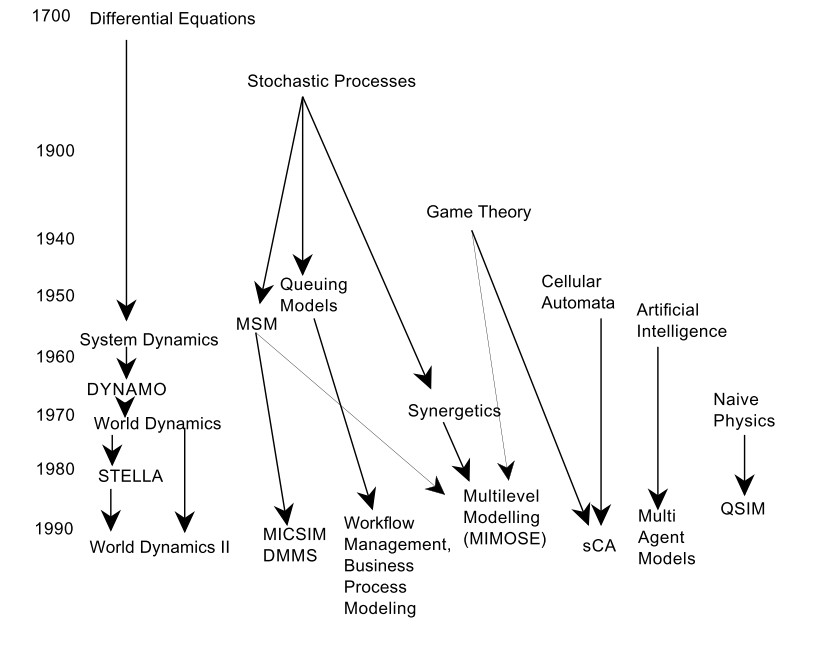
\includegraphics[width=.9\linewidth]{lineaire_figure.jpg}
  \end{sidecaption}
\end{figure}

Cette plongée à rebours dans l'histoire des pratiques de la simulation permet entre autres choses de constater l'ancienneté et la diversité des langages dédiés à la simulation (SIMSCRIPT, GPSS, DYNAMO, SIMULA, etc.), l'existence d'ouvrages et de conférences interdisciplinaires abordant très tôt les différents usages et problématiques soulevés par l'emploi de la simulation dans les sciences humaines et sociales \autocites{Shubik1960b,Shubik1960a, Borko1962, Guetzkow1962, Beshers1965, Guetzkow1972, Shubik1972, Morgan2004, Dutton1971}⁠⁠, et de saisir aussi l'importance des travaux des géographes informaticiens pionniers opérant dans ce contexte comme Marble \Anote{marble}, Pitts, Tobler, Tomlinson, Dacey, etc. \autocites{Marble2010, Marble1972}

Comme souvent pour les effets de mode, cette découverte de la simulation s'accompagne d'un certain emballement dans les usages et les promesses de résultats accompagnant l'usage de ces outils. On connaît bien par exemple les dégâts qu'ont pu faire dans cette discipline les promesses extravagantes sur la simulation et l'intelligence artificielle (\foreignquote{english}{ AI Winter }) (Crevier, 1993). %REF
Cet engouement initial pour les modèles (simulés ou non) sera donc pour certaines disciplines suivi d'une désaffection parfois renforcée par l'émergence de mouvements plus ou moins radicaux dénonçant, entre autre, le coût et la complexité des modèles de simulation construits, l'absence de modèles implémentés ou de résultats, la stérilité et/ou le réductionnisme d'une formalisation mathématique ou informatique trop simplifiante, les problèmes de sous-détermination ou d'équifinalité, voire en géographie l'aliénation philosophique et idéologique de ces nouveaux outils, pour n'en citer que quelques-uns. La géographie quantitative anglo-saxonne n'échappe pas à ces critiques dans le courant des années 1970, et voit même certains des plus proches défenseurs de la modélisation basculer dans l'opposition radicale, comme David Harvey par exemple.

Un certain nombre de ces critiques se rapportent à des problèmes issus des différentes dimensions institutionnelles, techniques, ou philosophiques prises par la \enquote{ problématique de la Validation }. La même famille d'arguments est toujours utilisée \autocites{Amblard2006, Waldherr2013}⁠ pour critiquer l'usage ou la portée explicative des modèles de simulation réalisés. Pour saisir quels sont les enjeux sous-jacents à cette question de la \enquote{ Validation } des modèles de simulation en géographie, il m'a semblé important de poursuivre et de clarifier ce débat en tenant compte à la fois de cette dimension historique et pluridisciplinaire du terme à travers son utilisation dans le courant de la \enquote{ \textit{Validation \& Verification} }, de la philosophie des sciences, et enfin du point de vue des modélisateurs en sciences humaines et sociales. 

\paragraph*{Le problème de la validation tel qu’amorcé par la cybernétique}

Dans un contexte marqué par l'échec des \foreignquote{english}{large scale models} noté dans les années 1960-1970 \autocite{Lee1973} et à côté du développement et de la diffusion parallèles de la micro-simulation, la construction de modèles urbains semble connaître une transformation qui va de pair avec la diffusion mondiale des premiers cadres d'analyse systémique introduits quelques années auparavant \autocites{Ackerman1963, Harvey1969, Berry1964a, Chorley1962, Haggett1965}⁠. Le modèle de simulation Urban Dynamics de Forrester (Forrester, 1969)⁠%REF
est considéré par de nombreux géographes comme un événement charnière cristallisant cette séparation entre les anciens modèles statiques et aspatiaux et les nouveaux modèles spatio-temporels \enquote{ complexes } \autocites{Batty1976, Batty2005}. Le point de vue de Forrester sur la Validation apporte un certain \enquote{ sang neuf } dans la réflexion sur les modèles urbains \autocite{Lee1973}⁠, car il met l'accent non plus sur la présence et la quantité de données dont il faudrait disposer en amont pour construire des modèles \autocite[355]{Batty1976}⁠ mais sur la viabilité d'une démonstration avant tout basée sur la mise en dynamique d'une structure causale, une vision compatible aussi avec l'établissement de modèles plus parcimonieux. Toutefois, comme le laisse supposer l'introduction de \textcite{Tobler1970a} \Anote{tobler_review} dans sa review du modèle, celui-ci vient surtout, dans les faits stimuler la critique d'une génération de géographes comme Batty ou Wilson ayant déjà pour partie intégré la leçon sur les qualités, mais aussi les défauts de toute cette génération précédente de modèles arrivant des Etats-Unis (Batty, 1971)⁠%REF
. Mais, même faux, les résultats contre-intuitifs portés par ce modèle de simulation démocratisent auprès d'un large public de politiques, de scientifiques et de planificateurs les périls (Berry, 1970)%REF
⁠ associés à la modélisation de ces systèmes complexes.

Il m'a paru intéressant d'articuler les réflexions encore empreintes de cybernétique portées par Forrester sur la \enquote{Validation}, avec celles existantes de façon plus générale dans la littérature à cette période. Par exemple, l'économiste Thomas Naylor ou le spécialiste en sciences politiques Charles F. Hermann \autocites{Naylor1966,Naylor1967, Naylor1969, Hermann1967} sont reconnus \autocites{Nance2002, Balci1986} ⁠pour avoir pris au sérieux cette problématique dès le milieu des années 1960, avec la volonté de garantir une certaine crédibilité dans les usages de cet outil simulation. Les ouvrages collectifs interdisciplinaires \autocites{Guetzkow1972, Dutton1971} \Anote{guetz} abordent d'ailleurs frontalement cette problématique au travers de la construction, ou de l'évaluation des modèles de simulation, et ceux-ci méritent à ce titre d'être réexplorés plus en détails afin d'être correctement cités au regard d'une littérature qui ne dit parfois pas beaucoup plus sur cette question. 

\paragraph*{Une plateforme construite pour tirer parti du calcul intensif}

La seconde partie de cette thèse traite de la réalisation d'une plateforme pour la construction et l'évaluation des modèles de simulation, avant tout guidée par la nécessité d'un accès plus démocratisé au calcul intensif chez les géographes. A l'image d'une science géographique construisant et diffusant ses connaissances de façon cumulative (Pumain, 2003, 2005) %REF
⁠, ce projet ne pouvait pas, il me semble, être abordé sans être replacé dans le fil d'une évolution des outils et des pratiques à la fois en géographie et en particulier au laboratoire Géographie-cités.

Depuis plus de 25 ans et dès le début des années 1980, l'utilisation innovante de ressources de calculs intensifs pour la géographie et la modélisation a été pensée, expérimentée puis théorisée par les géographes de l'école de Leeds (Openshaw and Abrahart, 2000; Openshaw, 1983; Turton I. et al., 1996; Turton and Openshaw, 1998)%REF
⁠. Malgré les efforts de ces derniers pour mettre en avant de façon plus pédagogique (Turton and Openshaw, 1998)%REF
 la faisabilité de ces usages au regard des grandes opérations de normalisation touchant le High Perfomance Computing (HPC) dans les années 1990, cette vision n'a jamais percolé en dehors d'un cercle restreint de géographes aux compétences géo-informatiques très avancées. Il s'agit alors d'identifier quels différents éléments ont pu freiner l'adoption de ce qui aurait pu être aussi en France un usage du calcul intensif se plaçant en continuité logique avec les pratiques des premiers géographes. Car, de façon assez équivalente aux usages rapportés par certains géographes informaticiens américains (Marble, 2010)⁠%REF
 , la plupart des pionniers géographes français sont venus à l'informatique par l'apprentissage difficile de la programmation, un usage répété et complexe de cette ressource dans les centres de calculs, et la mise en place de multiples collaborations interdisciplinaires, seule façon pour eux d'accéder à cette ressource dans les années 1970. Il y a donc eu des pratiques, des connaissances, des collaborations, des lieux associés à ces usages pionniers du calcul, et donc de la simulation, pour la géographie. \textit{La micro-informatique a-t-elle vraiment rendu obsolète la pratique des centres de calculs, ou existe-t-il d'autres raisons ? Que reste-il de ces usages aujourd'hui ?} Sur ce point les historiens géographes spécialistes de cette littérature ne semblent pas encore s'être saisis de cette thématique, même si on en trouve déjà quelques traces dans les derniers travaux sur la question \autocite{Cuyala2014}⁠. La récolte de différents témoignages permettra de donner une première visibilité à ces pratiques, en montrant notamment comment certaines d'entres-elles ont pu malgré tout se pérenniser, en dépit des fortes restructurations qu'a subi le paysage du calcul intensif en France dans les années 1990.

Le calibrage \Anote{railsback} des premiers modèles de simulation récupérés dans les années 1980 par l'équipe PARIS (Pumain et al., 1983, 1989; Sanders, 1984)%REF
⁠ nécessite l'usage d'algorithmes d'optimisation (descente de gradients) qui mobilisent pour leur exécution un usage intensif des ressources HPC alors disponibles. Même si cet essai ne permet pas d'obtenir le résultat escompté, il inscrit dans les pratiques ce besoin fondamental d'explorer les modèles, besoin dont on sait qu'il faudra un jour le combler. 

Le fait que nous nous trouvions dans une situation quasi-similaire presque trente ans plus tard, dans un projet interdisciplinaire mobilisant la construction et l'exploration de nouveaux modèles de simulation au travers d'une plateforme développée par des ingénieurs informaticiens spécialistes du calcul intensif, ne pouvait donc pas résulter du seul hasard, et s'inscrit assez logiquement comme la résurgence d'un besoin d'exploration des modèles plus systématique resté latent jusque là. De même que des logiciels de modélisation ont permis l'émergence de mouvements pour l'autonomie de géographes modélisateurs (Banos, 2013)%REF
⁠, il aura probablement fallu attendre l'émergence de logiciels tel que celui développé par les ingénieurs de l'ISC-PIF (OpenMOLE) pour que puisse se démocratiser dans notre discipline encore faiblement formée à l'informatique l'accès et l'usage à des ressources de calcul High Perfomance Computing (HPC) dont on a pourtant identifié depuis bien longtemps la nécessité. 

Cette contingence heureuse mérite toutefois qu'on s'y attarde un peu plus, ne serait-ce que pour comprendre la forme de cet objet commun ayant précipité ainsi cette collaboration entre deux parties aux objectifs, temporalités, exigences apparemment bien différenciés. 

\paragraph*{Une construction dans un contexte interdisciplinaire}

Les dernières réflexions sur l'interdisciplinarité montrent en effet \autocites{Pumain2005, Chapron2014}⁠ que quelque soit la méthode utilisée pour organiser et s'assurer de la réussite d'une activité de recherche interdisciplinaire, il est nécessaire de déconstruire les concepts et les objets engagés par les différentes disciplines pour que puissent émerger d'un processus de co-construction \autocite{Banos2013}⁠ les nouveaux formalismes, grilles et langages communs, et autres objets partagés à même de supporter, voire de catalyser, des enjeux scientifiques qui dépassent le cadre des disciplines prises isolément.

On aurait tort de penser cette déconstruction opérante sur le seul plan de la vie des idées, les outils étant également impactés, surtout lorsqu'une équipe de géographes est amenée à intégrer les projets d'ingénieurs informaticiens engagés depuis plusieurs années dans la réalisation d'une plateforme aux objectifs autonomes. Suite au constat en 2010 d'une convergence potentielle entre les deux projets, il a fallu pour que la coopération s'avère plus bénéfique encore, savoir se dessaisir d'un projet scientifique et technique conçu pour les besoins des géographes, à l'échelle d'une personne et d'une thèse \autocites{Rey2009, Louail2010}⁠, pour la réinventer au travers de nouveaux objectifs communs, en inter-dépendance avec une équipe d'ingénieurs forte de son propre calendrier et de ses propres objectifs de développement, au contact d'un projet déjà mature et complexe. 

L'insertion de mon travail dans ce processus interdisciplinaire se fait dans le remplacement progressif d'un objet par un autre, à la fois plus prometteur dans les évolutions qu'il propose au-delà du cahier des charges fixé initialement, mais aussi beaucoup moins maitrisé et maitrisable sans faire appel aux compétences de deux ingénieurs évoluant dans des temporalités de développement très différentes, ce qui ne sera pas sans causer certains inconvénients. \textbf{Il ne s'agissait donc plus de créer la plateforme, mais de l'intégrer, en appelant la construction de nouveaux outils et de nouvelles méthodes pour la construction et l'exploration plus systématique des modèles de simulation, dans un projet bénéfique aux deux parties} \autocite{Pumain2014}⁠.

\paragraph*{Les étapes de construction de la plateforme}

L'exploration des modèles de simulation devient l'objet de recherche par lequel transitent les préocupations communes aux deux équipes. Le travail s'organise sur deux fronts dans lesquels je suis inscrit comme développeur, avec la création de SimpopLocal d'une part, et d'autre part la construction parallèle des nouveaux outils à même de supporter l'exploration de celui-ci dans OpenMOLE. Le hasard a fait qu'il existait dans chacune des équipes originales une volonté de traduire l'exploration des modèles de simulation en s'appuyant sur l'utilisation d'algorithmes d'optimisation pris dans la famille des Algorithmes Evolutionnaires. C'est donc en repartant d'un premier framework nommé MGO, développé dans une version encore instable en 2010 à l'ISC-PIF, que cette première intégration de la plateforme prend place.

Entre 2010 et 2013, l'équipe se focalise sur la réalisation d'un premier prototype fonctionnel démontrant la faisabilité d'une exploration plus systématique du modèle de simulation SimpopLocal en utilisant OpenMOLE et MGO. Par extension, et c'est là une des forces de cette collaboration, la méthodologie et les outils développés sont mutualisés au sein d'OpenMOLE et deviennent par extension utilisables pour d'autres modèles de simulation \autocites{Schmitt2014, Reuillon2015} 
 
C'est sur la base de cette exploration systématique appuyée par le HPC et des Algorithmes Evolutionnaires que va se constituer dans notre équipe une nouvelle génération de modèles de simulation et de nouvelles méthodes de construction et d'exploration des modèles (Cottineau, 2014; Cottineau et al., 2015; Chérel, 2013)%REF
⁠. Ces développements se feront aussi en regard des nouvelles possibilités permises par l'usage facilité du HPC (Openshaw and Abrahart, 2000)⁠, mais aussi au travers d'une réflexion commune sur les questions épistémologiques associées à l'usage de ces nouveaux outils. 

J’ai souhaité introduire ce travail en présentant des éléments de contexte qui l’ont fortement contraint et inspiré. La rédaction de la thèse a obéi à deux motivations étroitement enchevêtrées : la première partie expose les cheminements des raisonnements relatifs à la modélisation et à la validation. J’ai mené cette enquête, qui n’était pas exigée par mes encadrants, et pour laquelle je ne disposais pas de formation particulière, pour satisfaire à une exigence intellectuelle ; la méthodologie que j’ai utilisée ne relève donc pas des canons de l’épistémologie ou de l’histoire des sciences, mais d’une remontée approfondie dans l’histoire des sources sur cette question, appuyée sur une bibliographie très abondante et des interrogations par voie écrite ou orale adressées à des acteurs majeurs de ce domaine. La seconde partie retrace la logique de construction et d’intégration d’une plateforme dans une perspective de géographe informaticien, selon des méthodes qui sont entièrement explicitées. La conclusion permet de faire le lien entre cette expérience de réalisation et les problèmes relevés dans la première partie, tout en tentant une évaluation à la lumière des réalisations les plus récentes de ce domaine de recherche très actif. 

% -*- root: These.tex -*-
\graphicspath{{FigureIntroduction/}}

\chapter{Introduction}
\label{sec:Introduction}

\epigraph {A human being should be able to change a diaper, plan an invasion, butcher a hog, conn a ship, design a building, write a sonnet, balance accounts, build a wall, set a bone, comfort the dying, take orders, give orders, cooperate, act alone, solve equations, analyze a new problem, pitch manure, program a computer, cook a tasty meal, fight efficiently, die gallantly.  Specialization is for insects. } { --- \textup{Robert Heinlein} Time Enough for Love}

\Anotecontent{smil_lund}{Qui donc a pensé à demander à Hägerstrand comment celui-ci avait formulé et programmé pour la première fois son modèle sur l'ordinateur SMIL à Lund ? \autocite{Hagerstrand1965}} 

\Anotecontent{exploration_marge}{Un travail d'exploration rendu possible par l'émergence d'outils pour questionner les marges de ce qui est en train de devenir un nouveau continent numérique dédié au patrimoine scientifique. Ces dernières années ayant vu l'expansion rapide de son volume, principalement du fait de la multiplication des campagnes de numérisation et de la modernisation des métiers et des outils d'archivages.}

\Anotecontent{marble}{Marble a écrit un chapitre dans l'ouvrage de Guetzkow publié en 1972, les deux étant à la même université à cette période, comme celui-ci me l'indique dans un échange privé : \foreignquote{english}{Actually, I was approached by Guetzkow about doing the article. As I recall, he was also on the faculty Northwestern University as I was at that time. }}

\Anotecontent{tobler_review}{\foreignquote{english}{This is a difficult, dangerous, important book. }}

\Anotecontent{guetz}{\foreigntextquote{english}[{\cite[6]{Guetzkow1972}}]{The disadvantages of modeling in general, including simulation, stem from the model's artificiality, abstraction or simplification, and idealization, and the consequent difficulties and dangers in making inferential leaps from a model to the real world. Questions of validity and inference in the model-building process are very important on both theoretical and pragmatic grounds.}}

\Anotecontent{railsback}{Selon \textcite[256]{Railsback2012}⁠, le calibrage des modèles de simulation recoupe trois objectifs : identifier le meilleur ajustement possible avec les données ; trouver les valeurs de paramètres que l'on ne peut pas définir empiriquement, en identifiant les valeurs de façon \enquote{ inverse } dans la recherche d'un meilleur ajustement possible du modèle aux données (\foreignquote{english}{inverse modelling}) ; et la mise en tension de la structure interne du modèle au regard du meilleur ajustement obtenu, ce qui rentre dans la catégorie des tests de robustesse.}

Ce projet de thèse s'inscrit dans la continuité d'un travail de stage initié au laboratoire Géographie-cités en 2009, sous la direction de Thomas Louail et Denise Pumain. C'est de ce moment là que date pour moi la découverte et l'apprentissage passionnants de la modélisation multi-agents, principalement au contact de la famille de modèles Simpop (Simpop1, Simpop2, Eurosim, SimpopNano). Ce projet démarré au début des années 1990 propose d'exemplifier sur différents territoires et pour différentes temporalités les principes d'une \enquote{ théorie évolutionnaire urbaine } \autocite{Pumain1997}.⁠⁠ 

Après quelques mois passés sur l'amélioration du modèle Simpop2, les problématiques déjà soulevées par les précédentes explorations du modèle par Thomas Louail et Clara Schmitt sont apparues clairement. La principale difficulté consiste à l’évaluation des modèles. Avec Thomas Louail nous avons formulé une première réponse à ces problèmes sous la forme d'un projet de plateforme géomatique pour l'automatisation et le partage des explorations de modèles. Intégrée comme un chapitre de perspective dans la thèse de Thomas Louail, cette proposition également reprise dans mon stage de fin d'étude se concrétise dans un projet de thèse financé à la fin de l'année 2009 \autocite{Rey2009} par le réseau R2DS (Réseau Francilien de Recherche sur le Développement Soutenable -un des domaines d’intérêt majeur de la Région Ile-de-France).

A ce même moment, Clara Schmitt, alors ingénieure agronome et titulaire d'un Master 2 recherche en géographie, commence également sa thèse en géographie. Nos deux projets sont conçus en partie de façon interdépendante. Clara propose dans son projet de thèse la réalisation d'un ensemble de modèles (SimpopLocal, SimpopNet, SimpopClim) pour évaluer la dynamique de systèmes de peuplements sous contrainte environnementale à différentes périodes de transitions \autocite{Schmitt2014}⁠. ⁠Mon projet de thèse se construit de façon assez naturelle en parallèle de la création l'un de ces nouveaux modèles (SimpopLocal), car la plateforme a besoin pour exister d'être instanciée au travers d'un cas d'utilisation. C'est ainsi que démarre cette expérience, avec mon inscription active dans la conception, la construction et l'exploration de ce modèle SimpopLocal au sein d'une petite équipe interdisciplinaire (Arnaud Banos, Clara Schmitt, Denise Pumain). Beaucoup de choses vont changer au cours des années qui suivent, avec le rapprochement dès 2010 de notre équipe avec un autre projet de plateforme (OpenMOLE) mené à l'Institut des Systèmes Complexes de Paris Ile-de-France (ISC-PIF), puis l'obtention en 2011 d'une bourse de l’ERC par Denise Pumain. Nous aurons l'ocasion de revenir en détails sur la nature de ces changements dans la partie 2 de cette thèse.

L’extrait de texte suivant, tiré de l'introduction d'un article de Amblard \autocite{Amblard2006},⁠ résume très bien cette situation imaginée, redoutée, et parfois vécue par toute une génération de modélisateurs évoluant au laboratoire Géographie-cités : 

\blockquote[\cite{Amblard2006}]{Une critique récurrente faite aux modèles multi-agents porte sur leur \enquote{ validation }. Il est ainsi fréquent, lors de l'exposé d'un modèle, que la question de la validation, qui se veut être la question piège dans ce domaine, soit posée, plongeant le conférencier dans un embarras bien visible.}

Avec une problématique de thèse axée sur la construction et l'évaluation des modèles, j’ai été amené très vite à explorer les multiples fondations de cette \enquote{ problématique de la Validation } pour mieux tenter d'en extraire les implications. Mais pour déméler les fils complexes de cette question (qu'est ce que la Validation?), et tenter d'en concevoir une réponse plus ancrée dans une discipline géographique qui n'est pas sans \enquote{ histoire }, il faudrait rendre compte de toute la volonté et l'expertise cumulées d'une équipe interdisciplinaire sur plusieurs années. Sans vouloir me substituer à cette voix commune, je propose d'aborder ici les tenants et les aboutissants d'une aventure en deux parties, entre théorie et pratique.

La première partie de cette thèse propose une lecture historique et théorique des problématiques posées par la question de la \enquote{ Validation } des modèles de simulation. Cette réflexion préalable s'est nourrie et développée au fil des années à l'interface de questions méthodologiques et informatiques posées de façon plus immédiate par la réalisation et l'évaluation nécessaires d'un modèle de simulation construit dans un contexte interdisciplinaire (SimpopLocal \autocite{Schmitt2015}). La seconde grande partie souligne ce point de vue plus \foreignquote{english}{ bottom-up } et les besoins de plateformes et d'intégrations qui en découlent, tout en replaçant ce travail et ces problématiques dans l'histoire plus globale d'une évolution des pratiques de modélisation en géographie. La conclusion propose une lecture critique des méthodologies existantes, aiguillée par les apprentissages méthodologiques et techniques qui résultent d’un suivi \enquote{ en temps réel } d’une littérature scientifique en évolution extrêmement rapide.  

\paragraph*{Une construction qui s’appuie sur une histoire de la modélisation}

Les sciences humaines et sociales s'inscrivent dans une tradition d'utilisation de l'informatique et de la simulation vieille de presque 60 ans, qui a produit des outils dont on oublie souvent qu'ils ont pu faire la une des journaux à cette époque, fascinant alors tout autant les sciences physiques que les sciences humaines. Or c'est une histoire pour laquelle il n'existe souvent que des témoignages assez concis sur les aspects techniques\Anote{smil_lund} et des synthèses partielles, abordées sous une perspective linéaire qui ne tient pas forcément compte de l'aspect cumulatif de ces développements techniques (voir le schéma de \autocite{Troitzsch1997} sur la figure \ref{fig:S_Troitzsch})⁠, ou restreintes à une seule discipline, par exemple en archéologie \autocite{Lake2013}, en géographie \autocite{Sanders2013}, ou en sociologie \autocite{Manzo2007}. La tâche pour traiter en détail un front aussi large de contributions sur une période aussi longue que 60 ans est évidemment difficile, voire impossible. Mais il m'a paru intéressant de rappeler de façon moins détaillée, mais sur une portée plus large, toute la diversité de ces premiers travaux de simulation en sciences humaines et sociales\interfootnotelinepenalty=10000\Anote{exploration_marge}.

\begin{figure}[h]
\begin{sidecaption}[Développement des approches contemporaines de la simulation pour les sciences sociales]{ Développement des approches contemporaines de la simulation pour les sciences sociales selon \textcite{Troitzsch1997}}[fig:S_Troitzsch]
 \centering
 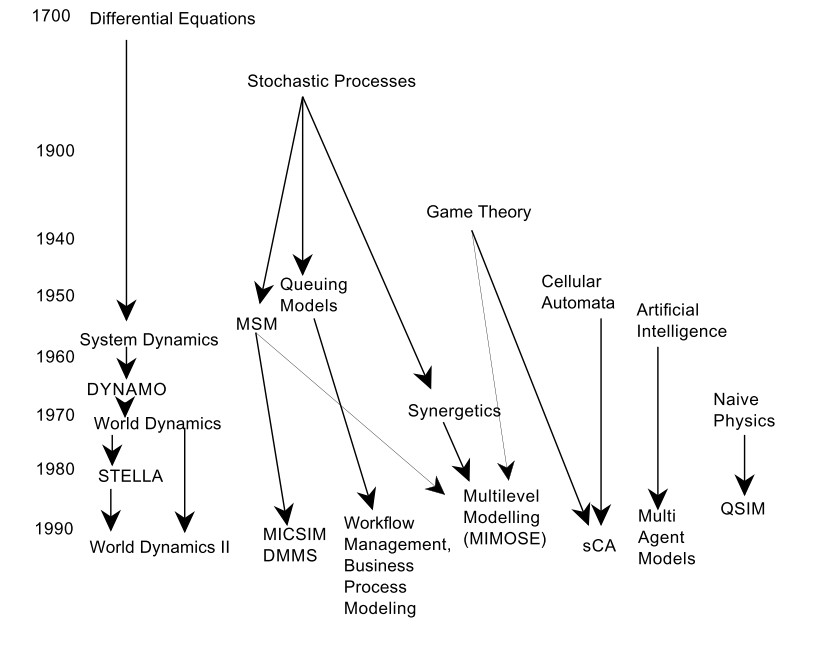
\includegraphics[width=.9\linewidth]{lineaire_figure.jpg}
  \end{sidecaption}
\end{figure}

Cette plongée à rebours dans l'histoire des pratiques de la simulation permet entre autres choses de constater l'ancienneté et la diversité des langages dédiés à la simulation (SIMSCRIPT, GPSS, DYNAMO, SIMULA, etc.), l'existence d'ouvrages et de conférences interdisciplinaires abordant très tôt les différents usages et problématiques soulevés par l'emploi de la simulation dans les sciences humaines et sociales \autocites{Shubik1960b,Shubik1960a, Borko1962, Guetzkow1962, Beshers1965, Guetzkow1972, Shubik1972, Morgan2004, Dutton1971}⁠⁠, et de saisir aussi l'importance des travaux des géographes informaticiens pionniers opérant dans ce contexte comme Marble\interfootnotelinepenalty=10000\Anote{marble}, Pitts, Tobler, Tomlinson, Dacey, etc. \autocites{Marble2010, Marble1972}

Comme souvent pour les effets de mode, cette découverte de la simulation s'accompagne d'un certain emballement dans les usages et les promesses de résultats accompagnant l'usage de ces outils. On connaît bien par exemple les dégâts qu'ont pu faire dans cette discipline les promesses extravagantes sur la simulation et l'intelligence artificielle (\foreignquote{english}{ AI Winter }) \autocite{Crevier1993}. 
Cet engouement initial pour les modèles (simulés ou non) sera donc pour certaines disciplines suivi d'une désaffection parfois renforcée par l'émergence de mouvements plus ou moins radicaux dénonçant, entre autre, le coût et la complexité des modèles de simulation construits, l'absence de modèles implémentés ou de résultats, la stérilité et/ou le réductionnisme d'une formalisation mathématique ou informatique trop simplifiante, les problèmes de sous-détermination ou d'équifinalité, voire en géographie l'aliénation philosophique et idéologique de ces nouveaux outils, pour n'en citer que quelques-uns. La géographie quantitative anglo-saxonne n'échappe pas à ces critiques dans le courant des années 1970, et voit même certains des plus proches défenseurs de la modélisation basculer dans l'opposition radicale, comme David Harvey par exemple.

Un certain nombre de ces critiques se rapportent à des problèmes issus des différentes dimensions institutionnelles, techniques, ou philosophiques prises par la \enquote{ problématique de la Validation }. La même famille d'arguments est toujours utilisée \autocites{Amblard2006, Waldherr2013}⁠ pour critiquer l'usage ou la portée explicative des modèles de simulation réalisés. Pour saisir quels sont les enjeux sous-jacents à cette question de la \enquote{ Validation } des modèles de simulation en géographie, il m'a semblé important de poursuivre et de clarifier ce débat en tenant compte à la fois de cette dimension historique et pluridisciplinaire du terme à travers son utilisation dans le courant de la \enquote{ \textit{Validation \& Verification} }, de la philosophie des sciences, et enfin du point de vue des modélisateurs en sciences humaines et sociales. 

\paragraph*{Le problème de la validation tel qu’amorcé par la cybernétique}

Dans un contexte marqué par l'échec des \foreignquote{english}{large scale models} noté dans les années 1960-1970 \autocite{Lee1973} et à côté du développement et de la diffusion parallèles de la micro-simulation, la construction de modèles urbains semble connaître une transformation qui va de pair avec la diffusion mondiale des premiers cadres d'analyse systémique introduits quelques années auparavant \autocites{Ackerman1963, Harvey1969, Berry1964a, Chorley1962, Haggett1965}⁠. Le modèle de simulation Urban Dynamics de Forrester \autocite{Forrester1969}⁠ est considéré par de nombreux géographes comme un événement charnière cristallisant cette séparation entre les anciens modèles statiques et aspatiaux et les nouveaux modèles spatio-temporels \enquote{ complexes } \autocites{Batty1976, Batty2005b}. Le point de vue de Forrester sur la Validation apporte un certain \enquote{ sang neuf } dans la réflexion sur les modèles urbains \autocite{Lee1973}⁠, car il met l'accent non plus sur la présence et la quantité de données dont il faudrait disposer en amont pour construire des modèles \autocite[355]{Batty1976}⁠ mais sur la viabilité d'une démonstration avant tout basée sur la mise en dynamique d'une structure causale, une vision compatible aussi avec l'établissement de modèles plus parcimonieux. Toutefois, comme le laisse supposer l'introduction de \textcite{Tobler1970a}\Anote{tobler_review} dans sa review du modèle, celui-ci vient surtout, dans les faits stimuler la critique d'une génération de géographes comme Batty ou Wilson ayant déjà pour partie intégré la leçon sur les qualités, mais aussi les défauts de toute cette génération précédente de modèles arrivant des Etats-Unis \autocite{Batty1971}
. Mais, même faux, les résultats contre-intuitifs portés par ce modèle de simulation démocratisent auprès d'un large public de politiques, de scientifiques et de planificateurs les périls \autocite{Berry1970}
⁠ associés à la modélisation de ces systèmes complexes.

Il m'a paru intéressant d'articuler les réflexions encore empreintes de cybernétique portées par Forrester sur la \enquote{Validation}, avec celles existantes de façon plus générale dans la littérature à cette période. Par exemple, l'économiste Thomas Naylor ou le spécialiste en sciences politiques Charles F. Hermann \autocites{Naylor1966,Naylor1967, Naylor1969, Hermann1967} sont reconnus \autocites{Nance2002, Balci1986} ⁠pour avoir pris au sérieux cette problématique dès le milieu des années 1960, avec la volonté de garantir une certaine crédibilité dans les usages de cet outil simulation. Les ouvrages collectifs interdisciplinaires \autocites{Guetzkow1972, Dutton1971}\Anote{guetz} abordent d'ailleurs frontalement cette problématique au travers de la construction, ou de l'évaluation des modèles de simulation, et ceux-ci méritent à ce titre d'être réexplorés plus en détails afin d'être correctement cités au regard d'une littérature qui ne dit parfois pas beaucoup plus sur cette question. 

\paragraph*{Une plateforme construite pour tirer parti du calcul intensif}

La seconde partie de cette thèse traite de la réalisation d'une plateforme pour la construction et l'évaluation des modèles de simulation, avant tout guidée par la nécessité d'un accès plus démocratisé au calcul intensif chez les géographes. A l'image d'une science géographique construisant et diffusant ses connaissances de façon cumulative \autocite{Pumain2003,Pumain2005}
⁠, ce projet ne pouvait pas, il me semble, être abordé sans être replacé dans le fil d'une évolution des outils et des pratiques à la fois en géographie et en particulier au laboratoire Géographie-cités.

Depuis plus de 25 ans et dès le début des années 1980, l'utilisation innovante de ressources de calculs intensifs pour la géographie et la modélisation a été pensée, expérimentée puis théorisée par les géographes de l'école de Leeds \autocites{Openshaw2000b,Openshaw2000, Openshaw1983,Openshaw1988,Turton1996,Turton1998, Diplock1996}⁠. Malgré les efforts de ces derniers pour mettre en avant de façon plus pédagogique \autocite{Openshaw2000} la faisabilité de ces usages au regard des grandes opérations de normalisation touchant le\textit{ High Performance Computing} (HPC) dans les années 1990, cette vision n'a jamais percolé en dehors d'un cercle restreint de géographes aux compétences géo-informatiques très avancées. Il s'agit alors d'identifier quels différents éléments ont pu freiner l'adoption de ce qui aurait pu être aussi en France un usage du calcul intensif se plaçant en continuité logique avec les pratiques des premiers géographes. Car, de façon assez équivalente aux usages rapportés par certains géographes informaticiens américains \autocite{Marble2010}, la plupart des pionniers géographes français sont venus à l'informatique par l'apprentissage difficile de la programmation, un usage répété et complexe de cette ressource dans les centres de calculs, et la mise en place de multiples collaborations interdisciplinaires, seule façon pour eux d'accéder à cette ressource dans les années 1970. Il y a donc eu des pratiques, des connaissances, des collaborations, des lieux associés à ces usages pionniers du calcul, et donc de la simulation, pour la géographie. \textit{La micro-informatique a-t-elle vraiment rendu obsolète la pratique des centres de calculs, ou existe-t-il d'autres raisons ? Que reste-il de ces usages aujourd'hui ?} Sur ce point les historiens géographes spécialistes de cette littérature ne semblent pas encore s'être saisis de cette thématique, même si on en trouve déjà quelques traces dans les derniers travaux sur la question \autocite{Cuyala2014}⁠. La récolte de différents témoignages permettra de donner une première visibilité à ces pratiques, en montrant notamment comment certaines d'entres-elles ont pu malgré tout se pérenniser, en dépit des fortes restructurations qu'a subi le paysage du calcul intensif en France dans les années 1990.

Le calibrage\Anote{railsback} des premiers modèles de simulation récupérés dans les années 1980 par l'équipe PARIS \autocites{Pumain1983,Pumain1989,Sanders1984}⁠ nécessite l'usage d'algorithmes d'optimisation (descente de gradients) qui mobilisent pour leur exécution un usage intensif des ressources HPC alors disponibles. Même si cet essai ne permet pas d'obtenir le résultat escompté, il inscrit dans les pratiques ce besoin fondamental d'explorer les modèles, besoin dont on sait qu'il faudra un jour le combler. 

Le fait que nous nous trouvions dans une situation quasi-similaire presque trente ans plus tard, dans un projet interdisciplinaire mobilisant la construction et l'exploration de nouveaux modèles de simulation au travers d'une plateforme développée par des ingénieurs informaticiens spécialistes du calcul intensif, ne pouvait donc pas résulter du seul hasard, et s'inscrit assez logiquement comme la résurgence d'un besoin d'exploration des modèles plus systématique resté latent jusque là. De même que des logiciels de modélisation ont permis l'émergence de mouvements pour l'autonomie de géographes modélisateurs \autocite{Banos2013}⁠, il aura probablement fallu attendre l'émergence de logiciels tel que celui développé par les ingénieurs de l'ISC-PIF (OpenMOLE) pour que puisse se démocratiser dans notre discipline encore faiblement formée à l'informatique l'accès et l'usage à des ressources de calcul \textit{High Perfomance Computing} (HPC) dont on a pourtant identifié depuis bien longtemps la nécessité. 

Cette contingence heureuse mérite toutefois qu'on s'y attarde un peu plus, ne serait-ce que pour comprendre la forme de cet objet commun ayant précipité ainsi cette collaboration entre deux parties aux objectifs, temporalités, exigences apparemment bien différenciés. 

\paragraph*{Une construction dans un contexte interdisciplinaire}

Les dernières réflexions sur l'interdisciplinarité montrent en effet \autocites{Pumain2005, Chapron2014}⁠ que quelque soit la méthode utilisée pour organiser et s'assurer de la réussite d'une activité de recherche interdisciplinaire, il est nécessaire de déconstruire les concepts et les objets engagés par les différentes disciplines pour que puissent émerger d'un processus de co-construction \autocite{Banos2013}⁠ les nouveaux formalismes, grilles et langages communs, et autres objets partagés à même de supporter, voire de catalyser, des enjeux scientifiques qui dépassent le cadre des disciplines prises isolément.

On aurait tort de penser cette déconstruction opérante sur le seul plan de la vie des idées, les outils étant également impactés, surtout lorsqu'une équipe de géographes est amenée à intégrer les projets d'ingénieurs informaticiens engagés depuis plusieurs années dans la réalisation d'une plateforme aux objectifs autonomes. Suite au constat en 2010 d'une convergence potentielle entre les deux projets, il a fallu pour que la coopération s'avère plus bénéfique encore, savoir se dessaisir d'un projet scientifique et technique conçu pour les besoins des géographes, à l'échelle d'une personne et d'une thèse \autocites{Rey2009, Louail2010}⁠, pour la réinventer au travers de nouveaux objectifs communs, en inter-dépendance avec une équipe d'ingénieurs forte de son propre calendrier et de ses propres objectifs de développement, au contact d'un projet déjà mature et complexe. 

L'insertion de mon travail dans ce processus interdisciplinaire se fait dans le remplacement progressif d'un objet par un autre, à la fois plus prometteur dans les évolutions qu'il propose au-delà du cahier des charges fixé initialement, mais aussi beaucoup moins maitrisé et maitrisable sans faire appel aux compétences de deux ingénieurs évoluant dans des temporalités de développement très différentes, ce qui ne sera pas sans causer certains inconvénients. \textbf{Il ne s'agissait donc plus de créer la plateforme, mais de l'intégrer, en appelant la construction de nouveaux outils et de nouvelles méthodes pour la construction et l'exploration plus systématique des modèles de simulation, dans un projet bénéfique aux deux parties} \autocite{Pumain2014}⁠.

\paragraph*{Les étapes de construction de la plateforme}

L'exploration des modèles de simulation devient l'objet de recherche par lequel transitent les préocupations communes aux deux équipes. Le travail s'organise sur deux fronts dans lesquels je suis inscrit comme développeur, avec la création de SimpopLocal d'une part, et d'autre part la construction parallèle des nouveaux outils à même de supporter l'exploration de celui-ci dans OpenMOLE. Le hasard a fait qu'il existait dans chacune des équipes originales une volonté de traduire l'exploration des modèles de simulation en s'appuyant sur l'utilisation d'algorithmes d'optimisation pris dans la famille des Algorithmes Evolutionnaires. C'est donc en repartant d'un premier framework nommé MGO, développé dans une version encore instable en 2010 à l'ISC-PIF, que cette première intégration de la plateforme prend place.

Entre 2010 et 2013, l'équipe se focalise sur la réalisation d'un premier prototype fonctionnel démontrant la faisabilité d'une exploration plus systématique du modèle de simulation SimpopLocal en utilisant OpenMOLE et MGO. Par extension, et c'est là une des forces de cette collaboration, la méthodologie et les outils développés sont mutualisés au sein d'OpenMOLE et deviennent par extension utilisables pour d'autres modèles de simulation \autocites{Schmitt2014, Reuillon2015} 
 
C'est sur la base de cette exploration systématique appuyée par le HPC et des Algorithmes Evolutionnaires que va se constituer dans notre équipe une nouvelle génération de modèles de simulation et de nouvelles méthodes de construction et d'exploration des modèles \autocites{Cottineau2015,Cottineau2014b,Cottineau2014a,Cherel2015,Reuillon2015, Schmitt2015, Schmitt2014}⁠. Ces développements se feront aussi en regard des nouvelles possibilités permises par l'usage facilité du HPC \autocites{Turton1998,Openshaw2000}⁠, mais aussi au travers d'une réflexion commune sur les questions épistémologiques associées à l'usage de ces nouveaux outils. 

J’ai souhaité introduire ce travail en présentant des éléments de contexte qui l’ont fortement contraint et inspiré. La rédaction de la thèse a obéi à deux motivations étroitement enchevêtrées : la première partie expose les cheminements des raisonnements relatifs à la modélisation et à la validation. J’ai mené cette enquête, qui n’était pas exigée par mes encadrants, et pour laquelle je ne disposais pas de formation particulière, pour satisfaire à une exigence intellectuelle ; la méthodologie que j’ai utilisée ne relève donc pas des canons de l’épistémologie ou de l’histoire des sciences, mais d’une remontée approfondie dans l’histoire des sources sur cette question, appuyée sur une bibliographie très abondante et des interrogations par voie écrite ou orale adressées à des acteurs majeurs de ce domaine. La seconde partie retrace la logique de construction et d’intégration d’une plateforme dans une perspective de géographe informaticien, selon des méthodes qui sont entièrement explicitées. La conclusion permet de faire le lien entre cette expérience de réalisation et les problèmes relevés dans la première partie, tout en tentant une évaluation à la lumière des réalisations les plus récentes de ce domaine de recherche très actif. 

% -*- root: These.tex -*-
\graphicspath{{FigurePartie1/}}

\chapter{Construction et évaluation de modèle en géographie}

\startcontents[chapters]
\Mprintcontents

%\epigraph{Nous sommes comme un patient qui sort d'un coma aussi long que la vie d'une étoile.
%Ce dont nous ne pouvons nous souvenir, nous devons le redécouvrir }{---  \textup{Robert Charles Wilson}  Axis}

\epigraph {La science, mon garçon, est faite d’erreurs, mais d’erreurs qu’il est bon de commettre, car elles mènent peu à peu à la vérité.} { --- \textup{Jules Verne} Voyage au centre de la Terre} 

\epigraph {La connaissance commence par la découverte de quelque chose que l'on ne comprend pas.  } { --- \textup{Frank Herbert}}

\epigraph {The most exciting phrase to hear in science, the one that heralds the most discoveries, is not \enquote{Eureka!} (I found it!) but \enquote{That's funny...} } { --- \textup{Isaac Asimov} } 

\pagebreak

% -*- root: These.tex -*-

% PARTI B1

\Anotecontent{artificial_societies}{ \hl{Un terme aujourd'hui désuet si on en crois chattoe brown ... }}

\Anotecontent{gilbert_confidence}{Le fait que \textcite{Gilbert2000a} fasse cette confidence dans un article intitulé \foreignquote{english}{Modelling Sociality : The View from Europe} dans l'ouvrage \foreignquote{english}{Dynamics in Human and Primate Societies} de Kohler et Gumerman \autocite{Kohler2000} n'est probablement pas anodin, et révèle l'existence passé d'une forme de cloisonement entre les deux foyers Européen et Américain sur ce sujet. Car face à l'ambition affiché de l'ouvrage d'Epstein et Axtell \foreignquote{english}{Growing artificial societies} \autocite{Epstein1996}, il est fort dommageable de voir que les projets européens, riche pourtant à cette époque d'un certain avancement sur le sujet, ne sont qu'à peine évoqués en introduction, la plupart des références n'allant pas en deça des années 1990. Le modèle Anasazi étant initialement inspiré des travaux sur Sugarscape \autocite{Rauch2002}, la participation des européens à cet ouvrage pourrait en définitive être interprété comme le signe d'une collaboration retrouvée.}

\Anotecontent{histoire_sugarscape}{Le journaliste \textcite{Rauch2002} a interviewé Joshua Epstein à ce sujet en 2002 : \foreignquote{english}{One day in the early 1990s, when he was giving a talk about his model of arms races, he met Axtell, who was graduate student. He wound up bringing Axtell to Brookings, in 1992. Not long after, Epstein attended a conference at the Santa Fe Institue [...] At Santa Fe juste then a big subject was artificial life, often called A-Life. \enquote{All of the work was about coral reefs, ecology, growing things that look like trees, growing things that look like flocks of birds, schools of fish, coral, and so on,} Epstein told me. \enquote{And I thought, jeez, why don't we try to use these techniques to grow societies?} Fired up, he returned to Brookings and discussed the idea with Axtell. There followed the inevitable napkin moment, when the two of them sat in the cafeteria and sketched out a simple artificial world in which little hunter-gatherer creatures would move around a landscape finding, storing, and consuming the only resource, sugar.} Le modèle est écrit sur sa propre base logicielle \textit{Object Pascal}, c'est à dire découplé d'une plateforme agent existante. Le code source n'est pas disponible en libre accès, et la plupart des versions que l'on trouve aujourd'hui sur les plateformes sont donc des réimplémentations basé sur la description faites des auteurs du modèle.}

\Anotecontent{varela_modele_ca}{Varela, Hersini, Bourgine \autocite{Bourgine1992} organise à Paris en 1991 la première conférence européenne ECAL sur la vie artificielle, mais il faut savoir que Varela développe aussi un modèle d'automate cellulaire appuyant sa théorie dès 1974 en Fortran, décrit par \textcite{McMullin1997b}. Sa \enquote{redécouverte} a permis de le sauvegarder sous une autre forme, dans un projet mené par \textcite{McMullin1997}.}

\Anotecontent{smith_bio}{Voici ce que Alvy Ray Smith, un informaticien pionnier dans le domaine de l'infographie, titulaire d'une thèse sur les automates cellulaires en 1970 et également connu pour ses travaux sur la représentation graphique des L-Systems, écrit sur son site internet vis à vis d'un état de l'art qu'il publie en \autocite{SmithIII1976} suite à ce qu'il apelle une des toutes premières conférences sur la VA : \foreignquote{english}{This is an extensive survey and bibliography of the field of CA (I was calling them \enquote{polyautomata} at the time) up to 1975. I added the words \enquote{Cellular Automata and} to the original title when I transcribed the original article into online form. It was originally written as the introduction to the German edition of Theory of Self-Reproducing Automata, by John von Neumann, edited (posthumously) by Arthur W Burks, University of Illinois Press, Urbana, 1968. Von Neumann performed the work, completed by Burks, in 1952-53. The German publishers never published the German edition, but gave me permission to publish my survey in the book listed above, the proceedings of a conference held in Noordwijkerhout, The Netherlands, Apr 1975. I like to call this conference ALife0 - for Artificial Life 0 conference - since it was the first attempt I know to cross-fertilization between biologists and computer scientists. Many of the players at this conference were present for ALife1, ALife2, etc - cf Simple Nontrivial Self-Reproducing Machines . Other participants at ALife0 were Karel Culik, Pauline Hogeweg, John Holland, Aristid Lindenmayer, and Stanislaw Ulam.}}

\Anotecontent{helmreich_IA}{L'Anthropologue \textcite[10]{Helmreich1998} ayant fait du SFI son terrain d'étude est tout à fait lucide sur cette question, et met le lecteur en garde au debut de sont ouvrage : \foreignquote{english}{Not all Artificial Life scientists are happy with how the recent history of the field is told, with how this shapes the terrain of inquiry, or with how the Santa Fe Institute is privileged in popular accounts [...] Many Europe-based researchers argue that Artificial Life was not created ex nihilo in New Mexico but has descended from tangled international lineages of cybernetics, systems theory, Artificial Intelligence, self-organization theory, origins of life research, and theoretical biology. The Chilean-born and Paris-based biologist Fransisco Varela [...] has argued that the materialization of Artificial Life in New Mexico has focused attention on overly computational views of life and that the naming of Artificial Life on the analogy to Artificial Intelligence has only made this more intense. U.S narrations of Artificial Life history are notorious in the international community for their erasure or marginalization of European and Latin American precedents and scientists, of transnational collaborations, and of the social, intellectual, and economic contexts that produced the science in some places and not others. [...] Indeed, my own decision to do field-work on the community at Santa Fe was powerfully guided by readings of popular science, and this book runs the risk of reinforcing the mainstream myth that \enquote{Artificial Life was born out of Zeus' head in Santa Fe, New Mexico, in the 1980's} -- as one Europe-based scientist sardonically summarized it to me.}}

\Anotecontent{echelle_optimization}{\foreignquote{english}{Evolutionary computation, the field of simulating evolution on a computer, provides the basis for moving toward a new philosophy of machine intelligence. Evolution is categorized by several levels of hierarchy: the gene, the chromosome, the individual, the species, and the ecosystem. Thus there is an inevitable choice that must be made when constructing a simulation of evolution. Inevitably, attention must be focused at a particular level in the hierarchy, and the remainder of the simulation is to some extent determined by that perspective. Ultimately, the question that must be answered is, \enquote{What exactly is being evolved?}} \autocite{Fogel1998}}

\Anotecontent{livret_CREA}{Le lecteur intéressé trouvera sur cette généalogie complexe de la notion des éléments de reflexion dans un livret édité par le CREA en 1985. Celui-ci relate un travail de trois ans de recherches sur la \enquote{Genealogie de l'auto-organisation} basé sur le dépouillements des archives du BCL. Ce livret traite des recherches réalisé par les chercheurs Isabelle Stengers, Pierre Livet, Pierre Lévy (lecture commenté des archives du BCL); et contient également des interviews menés par Isabelle Stengers de Fogelman-Soulié, Atlan, Von Foerster, Weisbuch, Varela. \autocite{CREA1985}}

\Anotecontent{pouvreau_livre1949}{\enquote{Ce dernier ouvrage est la synthèse des réflexions de Bertalanffy au cours des deux décennies passées, une systématisation des thèmes qu’il a jusqu’alors développés dans ses divers écrits. [...] L’originalité de ce livre par rapport à ses écrits antérieurs tient au fait que Bertalanffy, dans l’esprit du projet de \enquote{ systémologie générale } qui constitue désormais le cœur de ses préoccupations intellectuelles, ne se limite pas à y argumenter la nécessité d’un point de vue \enquote{ organismique } dans l’ensemble des domaines de la biologie – en particulier, à démontrer la pertinence et la fécondité des concepts de \enquote{ système ouvert } et d’\enquote{ ordre hiérarchique }. Il s’efforce aussi d’y établir l’évolution convergente de l’ensemble des sciences naturelles, sociales et humaines, ainsi que de la philosophie, vers une épistémologie centrée sur les concepts de système et d’organisation dynamique. La logique de Das biologische Weltbild est l’incarnation de l’idée fondamentale de Bertalanffy, et l’aboutissement d’un chemin initié dès sa thèse doctorale de 1926 : le dépassement de l’organicisme en direction du systémisme. Son livre se concluant en conséquence par un exposé des grandes lignes de sa \enquote{ systémologie générale }.}\autocite[46]{Pouvreau2006}}

\Anotecontent{taylor_openended}{\textcite{Taylor1999} parle pour ce cas de \textit{Open-Ended Evolution} : \foreignquote{english}{This term refers to a system in which components continue to evolve new forms continuously, rather than grinding to a halt when some sort of `optimal' or stable position is reached[...]Note that open-ended evolution does not necessarily imply any sort of evolutionary progress.[...]Also, by using the term `open-ended' I wish to imply that an indefinite variety of phenotypes are attainable through the evolutionary process, rather than continuous change being achieved by, for example, cycling through a finite set of possible forms.}}

\Anotecontent{taylor_reproduction}{Les deux termes réplication et reproduction sont souvent utilisés de façon synonyme mais renvoient en réalité à des études différentes, la première évoquant la capacité à reproduire une copie conforme, alors que la seconde renvoie au processus d'évolution naturel par la mise en oeuvre d'opération et de matériel génétique \autocites{Sipper1998,Taylor1999}}

\Anotecontent{renfrew_futur_archeology}{\foreignquote{english}{
There are the several elements that may come together to form this new morphogenetic paradigm in archaeology. The first is the concept of \enquote{system trajectory,} seen not merely in traditional system-theory terms, but in the dynamical sense facilitated by differential topology, including catastrophe theory. The second is the whole approach to self-organizing systems, pionereed by the \enquote{Brussels School,} which overlaps in some respects with the foregoing. The third is preoccupation with information flow, stressed by van der Leeuw, and cogently set out by Johnson in his chapter in this volume and in earlier publications. The fourth element is computer simulation, if it can be developed to cope with the complexity that we are dealing with in such a way as to escape the inflexibility of so many algorithms: The enthousiasm of Doran gives hope that it can.} \autocite[463]{Renfrew1982b}}

\Anotecontent{doran_86_DAI}{\foreignquote{english}{This paper reports initial experiments with a computer program which embodies an abstract model of a sociocultural system. The model displays a form of spontaneous collapse. Central to the model is the adoption and discard of mutually beneficial and cumulative contracts between the component actors of the system.[...] Allen(1982) has argued the relevance of \enquote{dissipatlve structures} and multiactor system concepts to the emergence of modern urban structure including global and local fluctuations. The CONTRACT model I describe here has a number of aspects in common with Allen's work. The CONTRACT model is based on three main assumptions. The first is simply that a sociocultural system may usefully be modelled in abstract computational terms. The second assumption is that a sociocultural system may be regarded as a distributed problem-solver, that is, it is solving the problem of how best to manipulate its environment in order to maximise its own \enquote{wellbeing}. The system is distributed in that there arc multiple loci of decision, actors, each of which has only partial knowledge, and in that the criterion of success, \enquote{wellbelng}, is itself distributed over the decision making loci and locally defined. The third assumption is that the knowledge which the problem-solver necessarily uses to solve its problem is to be identified with cumulative technological knowledge cooperatively deployed.} \autocite{Doran1986b}}

\Anotecontent{doran_82_DAI}{ \textcite{Doran1982} présente un modèle générique pour étudier les comportements d'un système socio-culturel. Pour simplifier, les agents sont amenés à se structurer pour exploiter au mieux les ressources d'un environnement; structure dont l'émergence doit être le reflet des interactions (contrat) et des capacités de cognitions (représentations, mémoire, objectif) propre à chacun des acteurs décidant de participer à cette économie. Voici le résumé qu'il donne à un des schéma qu'il présente \foreignquote{english}{A set of concurrent actors, the multiactor system, is structured by a pattern of contracts that effects exploitation of the environment. Each actor has its own simplified and typically distorted representation(\enquote{cognized model}) of the multiactor system and environment, and this representation determines its individual contract participation.} Doran fait références plusieurs fois à la possible adéquation  entre les problématiques rencontrés dans de telle systèmes sociaux et les progrès fait par l'intelligence artificielle dans la résolution de problèmes en environnement distribué : \foreignquote{english}{We need the concept of a set of processes that run concurrently, which in some suitable way exchange information(\enquote{pass messages}) and which thus collectively effect some required computation [...] Discovering ways in which a system of concurrent communicating processes can engage in heuristic human-like problem-solving is an important current research topic (for example Smith1979). This work is closely relevant to the study of the capabilities of sociocultural systems [...]}}

\Anotecontent{doran_85_DAI}{ \foreignquote{english}{In this paper I shall suggest that important problems of natural language and of individual and cultural knowledge mays usefully be approached by a computational route. Central to my argument will be the concept of a multi-actor system (sometimes called a \enquote{multi-agent system} in the research litterature). In artificial intelligence work, discussions of multi-actor systems typically envisage a collection of semi-autonomous computer controlled devices [...] which cooperate to perform some task in their common real world environment. However, an alternative is a single computer program which \textbf{simulates} actors in a modelled environment. In this case the aim is to use the study of a modelled multi-actor system to further understanding of real system -- both those that might be constructed and those human systems that are in existence around us.}\autocite[160]{Doran1985}} 

\Anotecontent{doran1982_reclamation}{ 
\foreignquote{english}{Several years ago \autocite{Doran1982}, I suggested that multiple agent systems (MAS) theory could form a basis of models of socio-cultural dynamics including the growth of social complexity. Since then MAS theory and distributed artificial intelligence (DAI) generally have developed substantially (\autocite{Bond1988} Gasser and Huhns 1989; Demazeau and Muller 1990 ) and now the idea of studying \enquote{societies} on computers is becoming not just tenable but fashionable - altought the emphasis is as yet largely on studying the properties of systems of abstract rather than realistic agents. In spite of this limitation, it now looks possible to develop my original suggestion in a more serious way, and briefly to compare it with the more prominent alternatives.} \autocite{Doran1997} 

Preuve de sa connaissance dans le domaine de l'intelligence artificielle et l'archéologie, ses articles précédents dans les années 1970, il se réfère très tôt et de multiple fois \autocites{Doran1992, Doran1994a} à l'article très connu sur les DAI de Alan Bond et Les Gasser en 1988 \autocite{Bond1988}. EOS est donc comme il le dit lui même dans \autocite{Doran1994a} en réalité un double projet qui lui permet de développer des questions de recherche au croisement de ces travaux en intelligence artificielle distribué et de l'archéologie, une trajectoire de recherche qu'il cultive depuis longtemps comme en témoigne déjà ces travaux (projet CONTRACT, EXCHANGE \autocite{Doran1986b}) au contact des nouveautés systémiques qui touche l'archéologie courant des années 1980. C'est donc dans la continuité de ces travaux que le projet EOS se met en place au début des années 1990, lui permettant d'activer cette triple synergie, entre un modèle archéologique de sociétés \autocite{Mellars1985}, des questionnements plus théoriques sociologiques, et le développement d'un \textit{testbeds} agent spécialisé (MCS/IPEM dévelopé en Prolog) au coeur de l'université d'ESSEX \autocite{Doran1992}}

\Anotecontent{note_bond_liens}{A noter sur ce point qu'il existe quand même des liens, et que déjà certains auteurs tel que \textcite{Bond1988} pointent déjà dans les années 1980 l'absence et la nécessité de la mise en place d'une boucle d'échange fructeuse entre disciplines autour des DAI : \foreignquote{english}{ Moroever, others have suggested that DAI may draw from and contribute to others disciplines, both absorbing and providing theorical and methodological fondations [ Chandrasekn81, Lesser83, Wesson81]} et d'ajouter plus loin la citation de Wesson en 1981: \foreignquote{english}{Fields of study heretofore ignored by AI : organization theory, sociology and economics , to name a few - can contribute to the study of DAI. Probably DAI advance these fields as well by providing a modelling technology suitable for precise specification and implementation of theories of organizational behavior } [Wesson81, p18] }

\Anotecontent{gilbert_date_clef}{Voici quelques jalons relevés au détour ( éditorial JASSS, page wikipédia, \autocite{Gilbert1999a} ) de sa prolifique bibliographie que lui même considère comme intéressant d'un point de vue historique pour la discipline.  

 \begin{itemize}
  \item Avril 1992, à Guilford (UK) s'ouvre le premier workshop nommé \foreignquote{english}{Simulating Societies} qui donnera lieu à un tout premier ouvrage \autocite{gilbert1994}. S'ensuivront plusieurs autres workshop un peu partout en Europe, comme celui de Sienne en Italie l'année d'après en juillet 1993, qui donnera lieu à la publication d'un deuxième ouvrage important en 1995 \autocite{Gilbert1995a}.
  \item En 1995, une conférence sur cette thématique est donné à Schoß Dagstuhl in Germany
  \item En 1997 le « first international conference on Computer Simulation and the Social Science» a lieu a Cortona en Italie. Celui çi est reconduit une deuxième fois en 1999 à Paris. 
  \item Au printemps 1998, Nigel Gilbert annonce le lancement de JASSS, premier journal éléctronique ayant pour thème la simulation en science sociale. Celui ci est ouvert à une publication largement inter-disciplinaire, et va s'imposer rapidement comme une référence dans ce microcosme qu'est encore la simulation en science sociale. La liste de diffusion \href{www.jiscmail.ac.uk/cgi-bin//webadmin?A0=simsoc}{@SIMSOC} voit également le jour cette année là.
  \item En 1999, Nigel Gilbert et Klaus G. Troitzsch publie le premier manuel  pour enseigner l'usage de la simulation à un plus large public. Depuis celui ci à été republié en 2005 \autocite{Gilbert2005}
 \end{itemize}
}

\Anotecontent{premier_ouvrage_gilbert}{Premier ouvrage publié sur ce thème par Nigel Gilbert \autocite{gilbert1994}, « Simulating Societies » réalise une première, sinon la première tentative de publication réunissant d'emblée autant d'acteurs usant du multi-agent dans leur disciplines. Reprenant la plupart des interventions réalisés àla conférence de Guilford en 1992, il réunit pour la première fois une multitude de point de vue en abordant le thème de la modélisation agent à la fois sur des aspects méthodologique \autocite{drogoul1994multi} et thématique avec la présentation de cas d'application dans divers domaines centrés autour de la simulation de modèles de «sociétés humaines» : archéologie, développement pour l'écologie, sociologie, etc. Si le livre n'est pas spécifiquement centré autour des ABM car d'autres types de modèles sont également présentés, il est clair dès la présentation des chapitres que c'est ce nouveau formalisme qui suscite le plus d'intérêt et de discussion. Si le formalisme agent est connu et reconnu par la suite pour sa capacité intégratrive dans des publications ultérieures, force est de constater dans cet ouvrage qu'il se présente déjà en 1994 comme un outil d'expression priviligié et immédiatement inter-disciplinaire. L'archéologie et l'anthropologie sont ici majoritaire, conséquence directe selon les auteurs de la capacité des chercheurs opérants dans ces disciplines a se positionner plus facilement comme observateur de notre société, facilitant ainsi l'extraction des éléments clés à intégrer dans les modèles. Cette remarque n'est pas anodine, et témoigne d'une observation faite par la suite en lisant ce premier chapitre introductif. Celui çi s'appuie sur un exemple de modèle archéologique (effondrement Maya) que les auteurs utilisent comme un fil conducteur pour desambiguiser un certain nombre de termes et de concepts propre au process de simulation , et table en conclusion sur un espoir non dissimulé d'arriver à formuler au travers  de ce travail un début de cadre de modélisation commun qui réunit les différentes approches existantes. Les réflexion sur un certain nombre de concepts montre un recul étonnant pour un premier ouvrage de réflexion sur la question. Ainsi, la partie \emph{key concepts in modelling and simulation} aborde de façon succinte les points suivants : définition d'un modèle, de simulation, explicitation de la différence entre modèle spécifié et modèle implementé, précisions sur la notion d'équifinalité des modèles, introduction à la validation.}

\Anotecontent{gilbert_EOS}{\foreignquote{english}{We can now examine an example of a simulation based on DAI principles to see whether it fits neatly into any of these theoretical perspectives on the relationship between macro and micro. I have been associated with the EOS (Emergence of Organised Society) project since its inception, although Jim Doran and Mike Palmer are the people who have done all the work (Doran et al. 1994, Doran \& Palmer, Chapter 6 in this volume).} \autocite[128]{Gilbert1995a}}

\Anotecontent{description_imagine_simulation}{\foreignquote{english}{What the computer offers is the possibility of writing a computer program which embodies, at some level of abstraction, precise specifications of all the relevant factors and of their interactions. These specifications need not embody any general laws, nor need they be mathematical in form, but each must be operationally complete so that together they enable the machine to generate a possible « history » of the island for the period. In addition, the program will generate an estimate of what the consequential archaeological record would be. Given such a program, the task of the archaeologist would be to vary the factor specifications, using his own experience and insight, until the events and deposits predicted by the machine best matched the actual excavation evidence. It would, in fact, be very much a case of « reconstructing the events at the scene of the crime» with the machine doing the tedious task of moving the « actors» and « scenery». For our specific example, the simulation might have as its main components:
\begin{itemize}
\item (a) a fixed « map» of the island including information about climate, vegetation and fauna, together with
\item (b) a specification of the type of settlement characteristic of each population, including information about its size, material products and demand upon the natural environment, and 
\item (c) rules specifying the dynamics of the system - the rules which determine where and when settlements are founded, when a settlement is abandoned, what forms of trade and conflict there are between settlements, and in what ways the material cultures of the populations evolve.
\end{itemize}
The machine would simulate the passage of time by repeatedly updating the map and the settlements « attached» to it by reference to the rules and specifications given - and the « history» so generated might well be both surprising and illuminating.}}

\Anotecontent{foerster_interview}{ Dans l'interview relate dans le cahier 8 du CREA \autocite[257-258]{CREA1985}, Foerster rapelle les motivations premières à l'origine du projet BCL, dont le projet initial ne visait pas forcément le rattachement au projet cybernétique, comme il a eu lieu par la suite : \enquote{ [...] Il y a eu trois conférences sur l'auto-organisation. Les deux premières organisées par Yovits et Cameron. La troisième année, c'est moi qui ai organisé la conférence sur \enquote{Principles of Self-Organizing Systems}, et cette fois Ross Ashby a participé à la rencontre. Pas avant. Ross n'était pas encore au BCL à l'époque. En fait, mon laboratoire, à l'origine, n'était pas consacré à la cybernétique. J'étais associé au groupe \enquote{cybernétique} de Macy, d'accord, mais j'ai apellé notre laboratoire non pas Cybernetic Computer Laboratory, mais Biological Computer Laboratory. Notre intérêt était indépendant des notions principales de la cybernétique qui, je dois le dire, m'apparaissaient à l'époque [...] assez peu fascinantes. Ce qui me fascinait c'était la causalité circulaire.[...] Ce qui m'intéressait vraiment, c'était les principes de computation des organismes vivants. [...] Nous n'étions pas des cybernéticiens. Chacun venait avec sa compétence. Ma compétence était en physique, et donc je jouais le rôle de l'avocat de la physique. Je prenais garde à ce que des lois de la physique ne soient pas violés. Il y avait donc un effort coopératif. C'est seulement plus tard que la cybernétique a pris un grand intérêt, [...] cinq ou six ans après le début du BCL, peut-être plus.}}

\Anotecontent{connexionisme_symbolisme}{\hl{A détailler avec Crevier, et ce que j'ai lu dans Restnick, plus citation du papier de Minsky sur le perceptron. La notion de connexionisme est en un certain sens intéressante, car mis à l'écart pendant des années, elle revient avec la notion forte de décentralisation en IA. L'analyse de Restnick sur ce point...}}

\Anotecontent{liaison_prigogine_foerster}{\hl{Voir ce que dit Foerster dans son interview au CREA...}}

%\Anotecontent{nature_ccs}{The program therefore developed its own core curriculum, establishing courses in automata theory, information and probability theory, analog and digital computers; and in natural language, psychology, and biology treated from an information-processing point of view. Students were also required to take a course in modern algebra and, when it became available, an advanced course in programming. \href{http://um2017.org/2017_Website/History_of_Computer_%26_Communications_Sciences.html}{@History of CCS}}

\Anotecontent{influence_turing}{bien peu de psychologues étaient disposés à s’intéresser à ce modèle qui s’opposait en fin de compte à toutes les écoles (behaviorisme, psychologie génétique, psychologie de la Gestalt, phénoménologie ou psychanalyse) 2 . C’est chez les chercheurs concernés par la construction d’automates de calcul que ce modèle suscita un vif intérêt. McCullough lui-même fut mis sur sa voie à la suite de la démonstration en 1936 par le logicien anglais Alan Turing de l’« isomorphisme » entre toute machine capable de réaliser un calcul fondé sur une procédure algorithmique et une « machine universelle » abstraite dotée d’un « programme » où figurent des instructions et des données que la machine lit sur un ruban de longueur infinie et où elle inscrit ses résultats\autocites[777-778]{Pouvreau2013}{Husbands2012}
}


\Anotecontent{mcculloch_ratioClub}{Une initiative que l'on peut rattacher à la relation complexe qu'il a tissé avec les nombreux membres du \textit{Ratio Club} fondé en 1949 par John Bates, et parmis lesquels vont figurer plusieurs scientifiques aux travaux notoires, dont plusieurs seront amenés à participer par invitation de McCulloch à des séjours aux Etats Unis : 

Des relations qui commence d'ailleur bien avant, car les travaux de Turing ont déjà traversé l'atlantique et marque d'une influence - peut être réciproque - les travaux de ce dernier avec ceux de  McCulloch, Pitts et Von Neummann. \Anote{influence_turing} Les travaux sur les neurones trouvant un écho positif dans les réflexions menés par Turing sur la  expose déjà une large correspondance avec certains des membres de ce groupe, membres qui par ailleurs n'ont pas attendu l'attribution officielle de Wierner pour esquisser des idées similaires à ce qui va devenir par la suite la \enquote{pensée cybernétique} 
, comme .  un groupe de cybernéticien anglais parmis lesquel figure Ashby (qui connait par ailleurs les écrits de McCulloch avant 1946 si on en croit la lettre de Bateson à Ashby daté de décembre 1946) entre 1949 et 1958, et dont l'influence scientifique de ses membres est aujourd'hui largement reconnu.

Spécifié que McCulloch entretient des rapports intéressants avec les différents membres, dont Ashby ne fut qu'un des membres parmis d'autres invités, preuve aussi de l'influence des penseurs anglais dans la structuration du mouvement cybernétique américain. Sur ce point on pourra se référer aux travaux répétés et très intéressant menés par \autocite{Husbands2012}, dont la plupart de ces réflexions sont tirés.}

\Anotecontent{sous_discipline_biologie}{ \enquote{ Surtout dans les années 1920 et 1930, les sciences biologiques furent en effet le lieu d’un mouvement dont la vocation était de réhabiliter la légitimité d’approches holistiques et néanmoins non métaphysiquement vitalistes de ce que Bertalanffy appelait les \enquote{ problèmes de la vie }, que ce soit d’une manière générale, à partir de considérations épistémologiques, ou sur un mode spécifique et empiriquement fondé, relatif à des problèmes bien circonscrits. Sept domaines furent plus spécifiquement concernés : l’embryologie, la théorie de l’évolution phylogénétique, la morphologie, la théorie de l’hérédité, l’étude du comportement de l’organisme individuel dans son environnement (soit selon la perspective du système formé par l’organisme et son environnement, soit selon la perspective de l’autonomie acquise par l’organisme par rapport à cet environnement) et, enfin, celle des relations entre espèces biologiques (biocénologie). } \autocite[153]{Pouvreau2013}}

\Anotecontent{ordre_desordre}{\enquote{En réalité, et Ashby fut explicite sur ce point en 1962, toute sa cybernétique justifiait l’idée de l’impossibilité d’une \enquote{auto-organisation} dans un système n’interagissant pas avec son environnement, les changements organisationnels devant tirer leur source de l’extérieur du système – il critiqua d’ailleurs la pertinence même du concept d’\enquote{ auto-organisation }, en toute rigueur \enquote{ auto-contradictoire } : le système improprement dit \enquote{ auto-organisé } détecte au moyen de ses échanges avec son environnement et sous la forme de perturbations affectant ses \enquote{ variables essentielles } la \enquote{ variété } de cet environnement, et ne peut gagner lui-même de \enquote{ variété } qu’en collectant de l’information sur cet environnement ou en tentant de contrôler les échanges de matière et d’énergie qu’il entretient avec lui. La théorie de la \enquote{ variété } apportait en fin de compte un fondement logico-mathématique à l’idée dont l’origine se trouve chez Fechner et que nous avons vue opposée par Bertalanffy à Schrödinger dès 1949, selon laquelle l’ordre \enquote{ organismique } ne doit pas être pensé comme \enquote{ issu de l’ordre }, mais comme émergeant \enquote{ épigénétiquement } du chaos selon des principes inhérents aux systèmes dynamiques : Ashby donna une impulsion significative à ce qui allait devenir, notamment par l’intermédiaire de Prigogine et Atlan, le fameux principe d’\enquote{ ordre à partir du bruit }} \autocite[800]{Pouvreau2013}}

\Anotecontent{conrad_model}{\foreignquote{english}{Largely because of the limits of memory, computational power, and available runtime (at Stanford University in the late 1960s there was only one IBM 360 mainframe for the entire campus), Michael’s first computer model of an evolving ecosystem was highly simplified and could represent only three hierarchical levels, the genetic, the organismic, and the population in a discrete, finite one-dimensional workld. Populations were limited to a few hundred individuals, and runs were limited to a few hundred generations. In keeping with the ineffability of fitness in real ecosystems, Michael was careful not to explicitly define any fitness function in his program, but allowed the reproductive success or failure of the biota to depend on the ecosystem interactions at every level so that reproduction, competition, and niche selection were subject to variation as the ecosystem itself evolved. For this reason, the behavior of the model was difficult to analyze in any detailed causal terms. }\autocite{Pattee2002}}

\Anotecontent{def_biomathematique}{\enquote{Afin de lever d’emblée toute ambiguïté quant à ce dont il sera question dans ce chapitre, une
définition s’impose au préalable : j’appelle \enquote{ biologie mathématique } (ou \enquote{ biomathématique }) ce qui se veut le parfait analogue pour la biologie de la physique mathématique : une entreprise de construction mathématique de concepts et de lois biologiques, où les mathématiques sont vouées à entretenir avec la biologie un rapport \enquote{ non plus descriptif, mais formateur } (Bachelard), ou mieux encore, \enquote{ constituant } (Lévy-Leblond). En ce sens, on ne peut parler de biologie mathématique ni dans le cas où les mathématiques n’ont pour fonction que de résumer statistiquement ou d’ajuster des données empiriques, ni dans celui où elles ne s’introduisent que par le biais des principes et lois physico-chimiques tels qu’on peut les mettre en œuvre dans l’analyse des objets biologiques.} \autocite[515]{Pouvreau2013}}

\Anotecontent{piaget_cloture}{\enquote{L’œuvre de Jean Piaget représente une étape cruciale dans l’histoire des modèles de la circularité biologique. En allant au-delà du contexte de l’embryologie, Piaget élabore une approche conceptuelle générale qui vise explicitement à cerner les spécificités de l’autodétermination biologique, par la jonction théorique entre circularité, autodétermination et dimension thermodynamique. En particulier, il développe un concept théorique fondamental dans cette tradition, celui de \enquote{ clôture organisationnelle } [...] , entendu comme complémentaire à celui d’ouverture thermodynamique de von Bertalanffy. L’objectif de Piaget est de rendre compatible l’idée d’un flux constant de matière et énergie entre l’organisme et l’environnement avec celle d’un ordre circulaire constitutif, qui maintient le système au cours du temps. Le concept de clôture de Piaget décrit la dynamique propre du vivant comme une forme d’autodétermination, dans le sens fondamental d’une connexion entre \textit{activité} et \textit{existence}, réalisée par un réseau circulaire de relations entre les composants de l’organisme, dont dépendent son unité et individuation.La distinction entre clôture organisationnelle et ouverture thermodynamique est le pivot théorique sur lequel les élaborations plus récentes de l’autodétermination biologique s’appuieront, plus ou moins explicitement. Cela vaut non seulement par rapport à la relation profonde entre stabilité de l’organisation et variations des processus sous-jacents, mais également en relation avec les interactions adaptatives de l’organisme avec l’environnement. Sur ce point, Piaget réinterprète et généralise les concepts d’assimilation et adaptation – initialement formulés par l’embryologie de Waddington – et décrit les interactions d’un organisme avec l’environnement en termes d’adaptation, conçue comme une assimilation des perturbations qui induit une \enquote{ autorégulation } interne (accommodation). Ainsi, l’organisation adapte le réseau circulaire de relations en fonction des perturbations, tout en maintenant la clôture qui réalise l’autodétermination} \autocite{Mossio2014}}

\Anotecontent{etude_pouvreau_mossio}{ A la suite d'un échange privé avec David Pouvreau daté du premier octobre 2014, il est apparu qu'une nette préfiguration de la notion de \enquote{cloture organisationelle} apparaisse dans les travaux de Bertalanffy au travers de sa théorie \enquote{bionomogénétique} de l'évolution.  Sur ce point, des travaux sont en cours, notamment avec le philosophe Matteo Mossio, pour tenter de reconstruire un historique de la notion de cloture qui tiennent compte à juste titre des travaux préalable, notamment ceux de Bertalanffy.
\textcite[619]{Pouvreau2013} définit et replace ce terme dans le contexte des débats sur l'évolution dans les années 1930 : \enquote{s’exerceraient des \enquote{ lois internes de forme }, ou \enquote {de structures }, qui s’expriment chez les organismes par des \enquote{ caractéristiques d’organisation } autonomes n’ayant \enquote{ rien à voir avec l’adaptation } ; des \enquote{ lois de la morphogenèse immanentes } qui codétermineraient l’évolution phylogénétique en opérant une sélection parmi les variations contingentes admissibles au titre de cette évolution, et conféreraient à celle-ci une \enquote{ directivité intérieure }. Typiquement \enquote{ organismique } par l’expression du principe d’\enquote{ activité primaire } qu’elle manifestait, il s’agissait d’une conception dynamique interprétant tout processus morphogénétique comme une \enquote{ réaction entre les ‘puissances’ inhérentes à l’organisme et les conditions extérieures }. Tout en demeurant sur le \enquote{ sol ferme } de la science, elle semblait à Bertalanffy fournir le cadre adéquat pour répondre à l’ensemble des critiques adressées aux théories \enquote{ sélectionniste } et \enquote{ mutationniste } }. 
L'\enquote{activité primaire} étant entendu selon \textcite[60]{Pouvreau2013} comme \enquote{Un schème anti-mécaniciste qu’il opposa tout au long de sa carrière à celui de la \enquote{ réactivité primaire }, selon lui à l’oeuvre aussi bien en biologie (par exemple dans la théorie des tropismes de Jacques Loeb ) qu’en psychologie (avec le behaviorisme) et en théorie de la connaissance (empirismes) – avec cette nuance importante que la combinaison de ce schème avec celui du \enquote{ système ouvert } faisait diverger Bertalanffy de la monadologie leibnizienne : \enquote{L’organisme, même sous des conditions extérieures constantes, donc en l’absence de stimulation extérieure, ne représente pas un système au repos, mais un système actif, mû intérieurement [innerlich gewegt] [...] Il faut considérer comme primaire l’activité autonome, et non la réactivité (le réflexe) }. C’est ce schème, en particulier, qui se devine en amont de sa conception épigénétique de la morphogenèse organique, lorsqu’il postula en 1928 afin d’expliquer ce phénomène un \enquote{ principe de formation immanent à l’organisation de la matière } } Ces définitions dont la complexité est apparente demande pour être mieux comprise de se plonger pleinement dans les écrits de \textcites[451-453, 158-161]{Pouvreau2013} se rapportant spécifiquement à la \enquote{bionomogénétique}.}


\Anotecontent{deux_principes_autoorganisation}{La théorie organismique de Bertalanffy fait état de deux grands principes, qui reprennent en unifiant les développements passés et multiples de nombreuses influences exposés en détail dans les publications de Pouvreau et Drack \autocites{Pouvreau2013, Pouvreau2007}. Le premier principe repris et travaillé dans la théorie de Bertalanffy est celui bien connu de système ouvert en équilibre de flux, éloigné de l'équilibre;  le deuxième moins connu est le principe de hierarchisation. Le couplage de ces deux principes ... on a une expression du vivant qui découle d'un principe d'auto-organisation, dont Pouvreau montre qu'il s'accord assez bien avec celui évoqué par Ashby dans son homéostat.}

\Anotecontent{Pouvreau_secondprincipe}{Le « second principe » de Bertalanffy était le schéma suivant de développement épigénétique d’un système, dont on peut remarquer qu’il correspond bien à ce que Chauvet a récemment posé comme une « caractéristique de la vie dans la matière ». Dans une étape « primaire », le système est « unitaire » : il forme une « totalité équipotentielle » ayant des capacités maximales de régulation. Aucune de ses parties n’y est encore investie d’une fonction spécifique. Dans un second temps survient un processus de « ségrégation » au cours duquel le système se « scinde » en sous-systèmes dont le développement spécifique ultérieur se prédétermine. Un processus de « différenciation progressive » engage alors chaque sous-système dans la voie de développement qui lui a été ainsi assignée. Il se caractérise par l’attribution de fonctions déterminées à ces sous-systèmes et la constitution de structures plus ou moins rigides. C’est un processus d’autonomisation relative et de spécialisation des parties et des processus, qui implique pour le système dans son ensemble une « perte de régulabilité » (ou de « plasticité ») et que Bertalanffy appela à partir de 1937 la « mécanisation progressive ». \autocite[476-477]{Pouvreau2013}}

\Anotecontent{piaget_mossio}{\enquote{L’oeuvre de Jean Piaget représente une étape cruciale dans l’histoire des modèles de la circularité biologique. En allant au-delà du contexte de l’embryologie, Piaget élabore une approche conceptuelle générale qui vise explicitement à cerner les spécificités de l’autodétermination biologique, par la jonction théorique entre circularité, autodétermination et dimension thermodynamique. [...] L’objectif de Piaget est de rendre compatible l’idée d’un flux constant de matière et énergie entre l’organisme et l’environnement avec celle d’un ordre circulaire constitutif, qui maintient le système au cours du temps. Le concept de clôture de Piaget décrit la dynamique propre du vivant comme une forme d’autodétermination, dans le sens fondamental d’une connexion entre activité et existence, réalisée par un réseau circulaire de relations entre les composants de l’organisme, dont dépendent son unité et individuation. La distinction entre clôture organisationnelle et ouverture thermodynamique est le pivot théorique sur lequel les élaborations plus récentes de l’autodétermination biologique s’appuieront, plus ou moins explicitement. Cela vaut non seulement par rapport à la relation profonde entre stabilité de l’organisation et variations des processus sous-jacents, mais également en relation avec les interactions adaptatives de l’organisme avec l’environnement. Sur ce point, Piaget réinterprète et généralise les concepts d’assimilation et adaptation – initialement formulés par l’embryologie de Waddington – et décrit les interactions d’un organisme avec l’environnement en termes d’adaptation, conçue comme une assimilation des perturbations qui induit une « autorégulation » interne (accommodation). Ainsi, l’organisation adapte le réseau circulaire de relations en fonction des perturbations, tout en maintenant la clôture qui réalise l’autodétermination} \autocite[12]{Mossio2014}}

\Anotecontent{terme_bioinformatique}{Paulien Hogeweg définit son objet de recherche \foreignquote{english}{on multilevel evolution aims to understand how different levels of selection, complex genotype phenotype mapping, and interactions over different timescales contribute to the evolution of complexity at the level of individuals and/or ecosystems.} On comprend pourquoi ces travaux ont eu autant d'impact du coté de la biologie, de l'écologie \autocite{Hogeweg1988}, que de l'informatique \autocites{Hogeweg1979, Hogeweg1983, Drogoul1993}. Dans cet extrait d'article \autocite{Hogeweg2011} elle témoigne de l'origine du mot \enquote{bioinformatique} début 1970. Un terme qui, au contraire de son usage actuel \autocite{Giavitto2002}, se rapproche initialement en bien des aspects de ce que \textcite{Giavitto2002} décrit comme ce processus d'aller retour entre les deux approches de \textit{Biological computing} et \textit{Computational Biology} : \foreignquote{english}{In the beginning of the 1970s, Ben Hesper and I started to use the term \enquote{bioinformatics} for the research we wanted to do, defining it as \enquote{the study of informatic processes in biotic systems}. [...] It seemed to us that one of the defining properties of life was information processing in its various forms [...] At a minimum, we felt that that information processing could serve as a useful metaphor for understanding living systems. We therefore thought that in addition to biophysics and biochemistry, it was useful to distinguish bioinformatics as a research field (or what we termed a “work concept”).[...] 
While evolutionary models mainly dealt with invasion of mutants and changing allele frequencies, the question of how evolution leads to complex organisms was not addressed. [...] To meet the challenge of a \enquote{constructive evolutionary biology} became another long-term goal of bioinformatics as we envisioned it. Research in artificial intelligence at this time was exploring new representations of information processing systems, often inspired by biological systems, [...] demonstrating the power of an individual self-centered approach to generating and/or understanding more global structures. We felt that the re-introduction of biologically inspired computational ideas back into biology was needed in order to begin to understand biological systems as information processing systems. In particular, a focus on local interaction leading to emergent phenomena at multiple scales seemed to be missing in most biological models.[...] In short, under the heading of bioinformatics we wanted to combine pattern analysis and dynamic modeling and apply them to the challenge of unraveling pattern generation and informatic processes in biotic systems at multiple scales.} \autocite{Hogeweg2011}}

\Anotecontent{conrad_explanation}{\foreignquote{english}{\textcite{Conrad1970} also studied general properties of evolution systems but from a different perspective that involved the simulation of a hierarchic ecosystem. A population of cell-like individual organisms placed in an array of environmental cells was subjected to a strict materials conservation law that induced competition for survival. The organisms were capable of mutual cooperation, as well as executing biological strategies that included genetic recombination and the modification of the expression of their genome. No fitness criteria were introduced explicitly as part of the program. Instead, the simulation was viewed as an ecosystem in which genetic, individual, and populational interactions would occur and behavior patterns would emerge.}\autocite[62]{Fogel2006b}}

\Anotecontent{patte_deception}{\foreignquote{english}{The hope of \enquote{strong} artificial life was stated by Langton : \enquote{We would like to build models that are so lifelike that they would cease to be models of life and become examples of life themselves.} Very little has been said at this workshop about how we would distinguish computer simulations from realizations of life, and virtually nothing has been said about how these relate to theories of life, that is, how the living can be distinguished from the non-living. The aim of this paper is to begin such a discussion.} \autocite[63]{Pattee1988}}

La géographie est partie prenante des bouleversements considérables introduits par la numérisation dans l’ensemble des pratiques scientifiques depuis à peine deux décennies, et cela à plusieurs titres. Les manifestations les plus évidentes tiennent à la prolifération des informations individuelles \enquote{géolocalisées} désormais disponibles sur toutes sortes de support, et notamment, ce qui est entièrement nouveau, en situations de mobilité \autocite{FenChong2012}. Les dispositifs techniques de repérage comme le GPS et l’ouverture des systèmes d’information géographique à l’interactivité avec l'évolution permanente des technologies sur Internet donnent lieu au développement d’une \enquote{géographie volontaire} \autocite{Goodchild2007}, qui conduit à diffuser auprès du grand public des pratiques et des savoir-faire jusqu’ici réservés aux professionnels. Le très grand nombre des institutions privées ou publiques qui partagent ce nouvel engouement pour l’inscription spatiale de leurs activités, tout comme la croissance fabuleuse des \enquote{ réseaux sociaux } sur Internet  contribuent à l’immense développement de ce qu’il est convenu d’appeler, sans traduction en français, les \textit{ big data }. Ces masses de données très labiles, évoluant souvent en temps réel, qu’il est relativement facile de collecter à différents niveaux d’agrégation, posent de nouveaux défis aux géographes en termes de traitement de ces informations, tout autant qualitatives que quantitatives.

Les méthodes classiques de résumé des connaissances par la modélisation et la visualisation doivent être considérablement transformées pour s’adapter à cette nouvelle donne. Mais il serait dommageable de ne pas appuyer notre réflexion sur les pratiques passées pour dessiner un horizon des transformations à venir. Avant d’en arriver au propos de cette thèse, il nous semble indispensable d’opérer un retour sur les expériences de modélisation qui ont été conduites depuis plus de soixante ans dans le cadre paradigmatique général de la systémique. Notre sujet de thèse et notre hypothèse de recherche principale s’inscrivent en effet dans une longue histoire collective dont il nous faut repérer les forces et les faiblesses afin de construire une grille d'évaluation à même de justifier cette démarche que nous avons adoptée.

% -*- root: These.tex -*-


\section{L'entrée de la simulation comme méthode pour les sciences sociales}

L'effort militaire états-unien a non seulement entrainé dans ses retombées le développement des outils informatiques mais aussi l'institutionnalisation d'entreprises de connaissances appuyées sur ces nouveaux outils tels que le MIT, ou dans un autre genre la RAND corporation, et autres diverses formations.

Ces institutions nouvelles ont largement contribué à susciter des rencontres interdisciplinaires qui vont favoriser la pénétration des idées de l'école néo-positiviste puis du paradigme systémique, jusque dans les sciences humaines et sociales.

En parallèle, les lois de Boltzman pour la thermodynamique, ou le principe d’indétermination d'Heisenberg pour la mécanique quantique, viennent secouer le dogme du déterminisme scientifique hérité de la pensée mécanique, et plongent de nombreuses disciplines en \enquote{crises} \autocite[20-23]{Pouvreau2013}. Cette remise en cause est contemporaine de l'émergence d'une pensée \enquote{holiste} (ou pensée de la \enquote{totalité}) qui se construit en confrontation avec la démarche réductionniste classique.

C'est dans ce contexte que l'irruption de l'ordinateur (section \ref{sec:apparition_outil_informatique}) vient bouleverser en tout point le rapport des scientifiques aux données. Si les données de recensements focalisent les premiers travaux interdisciplinaires, les usages s'étendent rapidement à de nouvelles thématiques propres aux différentes disciplines. Un usage particulier de l'ordinateur va accrocher la curiosité de plusieurs chercheurs en sciences humaines et sociales. Cette capacité de celui-ci à supporter dans un environnement virtuel des expériences d'un genre nouveau, permettant de projeter des hypothèses dans le temps et dans l'espace pour observer l'évolution de systèmes dont on ne peut étudier leur comportement dans la réalité.

Afin de donner aux lecteurs des éléments de compréhension pour poursuivre la lecture du manuscrit, la partie suivante (section \ref{sec:apparition_simu_science_sociales}) expose quelques premières définitions générales sur les modèles et la simulation (section \ref{ssec:rapell_termes_generiques}) qui tiennent à la fois compte du contexte historique propre à leur apparition, mais s'intègrent également dans des grilles de classification plus récentes et volontairement plus englobantes, fruit des longs travaux menés par des épistémologues spécialistes de la simulation.

Après avoir constaté l'usage très ancien des modèles de simulation pour l'expérimentation, cet engouement sera précisé par la collecte de nombreuses références dans de multiples disciplines des sciences humaines et sociales (section \ref{ssec:engouement_sciencesociale}); autant de pointeurs pour qui voudra poursuivre ses recherches dans ce vaste océan bibliographique, dominé par de nombreuses références croisées du fait de l'interdisciplinarité et de la position centrale affichée par quelques auteurs.

En géographie, la découverte des modèles de simulation coïncide avec l'établissement d'une véritable \enquote{révolution quantitative} (section \ref{sec:premier_modele_geo}), où l'usage de l'ordinateur accompagne, et rend possible même, cette transformation de la discipline voulue par une partie des géographes. C'est dans cette période 1960-1970 d'abondance des modèles (section \ref{ssec:revol_modele} ) que les premiers modèles de simulation émergent du fait de courants qui semblent diverger dans leurs intérêts : les planificateurs américains appuyés par la \textit{RAND corporation}\Anote{rand}, et les universitaires pionniers quantitativistes américains et suédois. L'occasion de voir ici quelles redéfinitions des termes sont proposées par les géographes, et de présenter plus en détail les acteurs de ces deux courants de modélisation.

Il s'ensuit une crise de confiance envers les outils  (section \ref{sec:critiques_simulation}), et plus particulièrement envers la simulation, qui touche les disciplines des sciences sociales (section \ref{ssec:disciplines_touches}) à des dates, des degrés et pour des raisons très différentes. La géographie (section \ref{ssec:crise_mutation}), bien que touchée, elle aussi, dans le courant des années 1970 par des critiques sur ses outils, ses méthodologies, ses résultats présente toutefois dans ses rangs la présence des éléments actifs d'une transformation (auteurs, publications, etc.) qui laisse deviner pour les années suivantes un changement de paradigme explicatif sur lequel nous reviendrons plus en détail dans la section \ref{ssec:transition_annee70}. Un glissement plus qu'une rupture, qui ouvre de toutes nouvelles perspectives thématiques, méthodologiques et techniques aux futurs géographes modélisateurs. Ces mêmes modélisateurs qui apparaissent un peu partout sur la planète, faisant suite à l'essaimage de cette révolution à l'international. Les Français découvrent brutalement dans les années 1970 ce bloc de 15 années d'expériences - positives et négatives - acccumulées par les pionniers. On parlera donc plutôt ici d'une transformation que d'une véritable crise, les modèles de simulation n'ayant jamais réellement disparu de la discipline.

Cette transformation ne change rien toutefois aux différentes problématiques ayant freiné l'adoption de la simulation dans de nombreuses disciplines, au contraire la \enquote{problématique de la Validation} qui en ressort se renforce même un peu plus avec la découverte de cette complexité à l'oeuvre dans les systèmes étudiés. Un facteur supplémentaire venant complexifier un peu plus les possibilités d'explorations de ces modèles, les méthodes algorithmiques et les capacités informatiques nécessaires s'avérant toute deux insuffisantes (section \ref{ssec:limitation_techniques_methodologiques}). Le chapitre \ref{sec:constante_problematique} traitera plus en détail les implications de ce dernier point avec des définitions et l'étude plus précise de cette transformation à l'oeuvre dans la façon de penser la construction des modèles de simulation.


%Ainsi malgré l'évolution et la démocratisation des outils informatiques et des plateformes de modélisation, l'accès à la ressource informatique (plateforme outils, formations limités, puissawnce disponibles) continue par la suite d'être un facteur limitant pour le développement de modèles plus complexes, mais aussi pour le calibrage et l'exploration efficace des comportements exprimés par ceux-ci, qui nécessite des compétences bien au delà du bagage technique initial des géographes.

%Il manque l'écologie, cf unwin1992 121


\subsection{Irruption de l'outil informatique }
\label{sec:apparition_outil_informatique}

%GUllahorn cite le recueil
%Supprime l'histoire du BIG DATA , qui est un anachronisme plutot >>

L'accumulation et l'exploitation de données numériques sont des problématiques récurrentes pour les géographes et les sciences humaines en général. Ainsi depuis les années 1950-1960 les spécialistes de sciences humaines et sociales ont régulièrement signalé l'importance de l'outil informatique pour le traitement de leurs données désormais informatisées, notamment depuis les premières grandes récoltes de données informatisées sur la population. \autocites{Kao1963, Hagerstrand1967b}[386]{Barnes2011}.

On pourra citer à ce propos \textcite{Gullahorn1966} lorsqu'il pointe l'importance pour les sciences humaines et sociales du recueil \textit{Computer methods in the analysis of large-scale social systems} qui retrace les discussions issues d'un des tous premiers grands rassemblements interdisciplinaires organisés par le MIT. Cette conférence pilotée par un sociologue de la section \foreignquote{english}{Urban Studies} du MIT \autocite{Beshers1965} propose de faire le point sur les nouvelles méthodologies et techniques quantitatives et leurs utilisations dans les différentes disciplines en sciences sociales, avec cette volonté marquée de reprendre le contrôle sur la construction des modèles\Anote{ptvuebesher}, afin de faire face à ce qui apparaissait comme une manne de données nouvelles, les données américaines de recensement \textit{U.S Census}. Une question brûlante d'actualité à l'ère du \textit{Big data}, car cinquante ans après, et des centaines d'innovations techniques plus tard, peut-on enfin dire que les scientifiques ont pris le plein contrôle de leurs données et des outils associés permettant la construction des modèles ?

\begin{figure}[!htbp]
\begin{sidecaption}[Le champignon informationnel de Frédéric Kaplan]{Le \enquote{champignon informationnel} proposé par Frédéric Kaplan est révélateur de l'augmentation du champ d'expérimentation rendu possible par la numérisation des données (\textit{Digitization}), puis la simulation numérique (\textit{Simulated information}). Pour les données les plus anciennes, il est proposé d'extrapoler avec l'aide des historiens les informations très lacunaires dont on dispose pour reconstruire par simulation les données manquantes, et produire ainsi des scenarii historiques crédibles : \enquote{Par exemple, un carnet de bord d’un capitaine de navire vénitien nous indique bien plus qu’un itinéraire particulier, il nous informe sur les routes commerciales d’une époque. De la même manière, une gravure représentant une façade vénitienne nous décrit bien plus que ce bâtiment en particulier, mais nous renseigne sur les grammaires architecturales utilisées à cette époque particulière. Les historiens extrapolent très souvent de cette façon. Il s’agit simplement de formaliser et systématiser cette démarche.}}[fig:I_Champi]
 \centering
 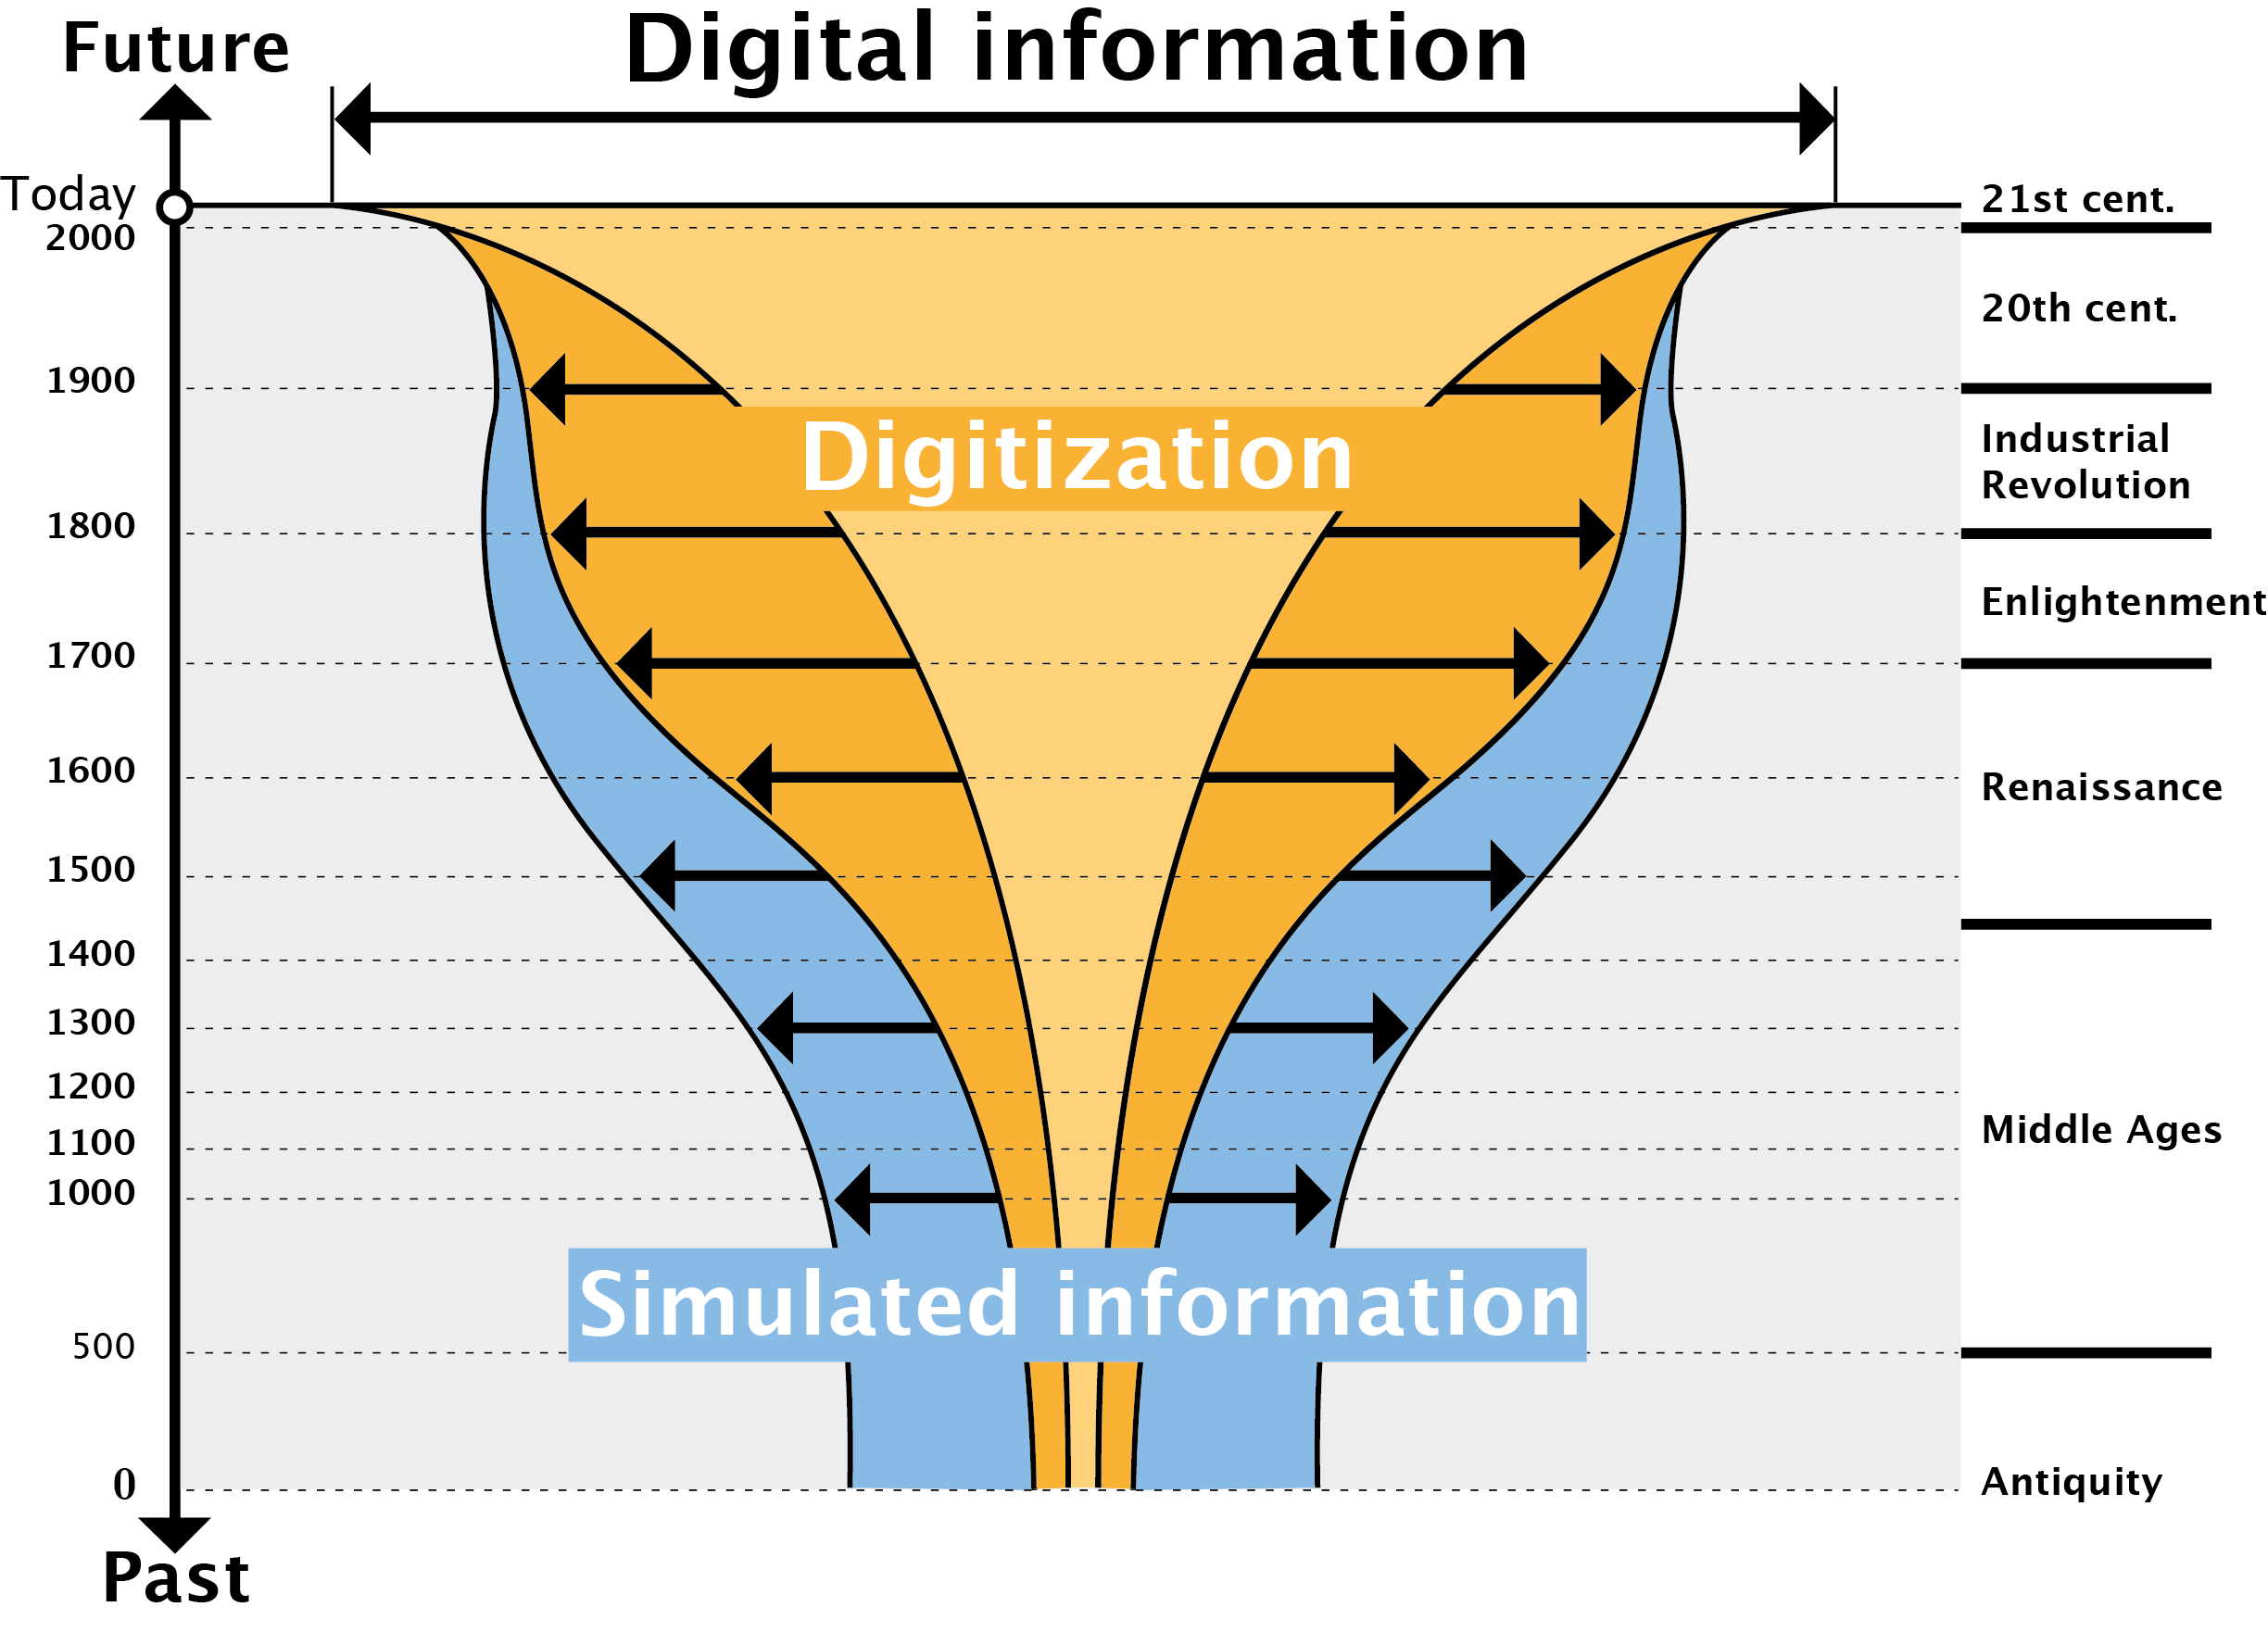
\includegraphics[width=.8\linewidth]{champignonKaplan.png}
  \end{sidecaption}
\end{figure}

Mais ce serait une erreur que de limiter l'application de ces nouveaux outils aux seuls stockages numériques récents, et ne pas citer l'importance du volume de connaissances accumulées ces derniers siècles par certaines sciences sociales telles que l'archéologie ou encore la géographie. Les lacunes dans l'information sont depuis longtemps une problématique récurrente pour de nombreuses disciplines en sciences humaines et sociales. L'outil computationnel a permis, dès lors qu'il a été disponible, d'envisager de combler ces lacunes efficacement, comme tente de le résumer la figure \ref{fig:I_Champi} \Anote{kaplan} de Frédéric Kaplan.

%\begin{figure}[tb]
%\raggedright
%\begin{sidecaption}{This is a subcaption just for illustration purposes. This is a subcaption just for illustration purposes.
%Champignon Informationnel de Frédéric Kaplan. Page number is \LARGE\textbf{\thepage}}[fig:test]
%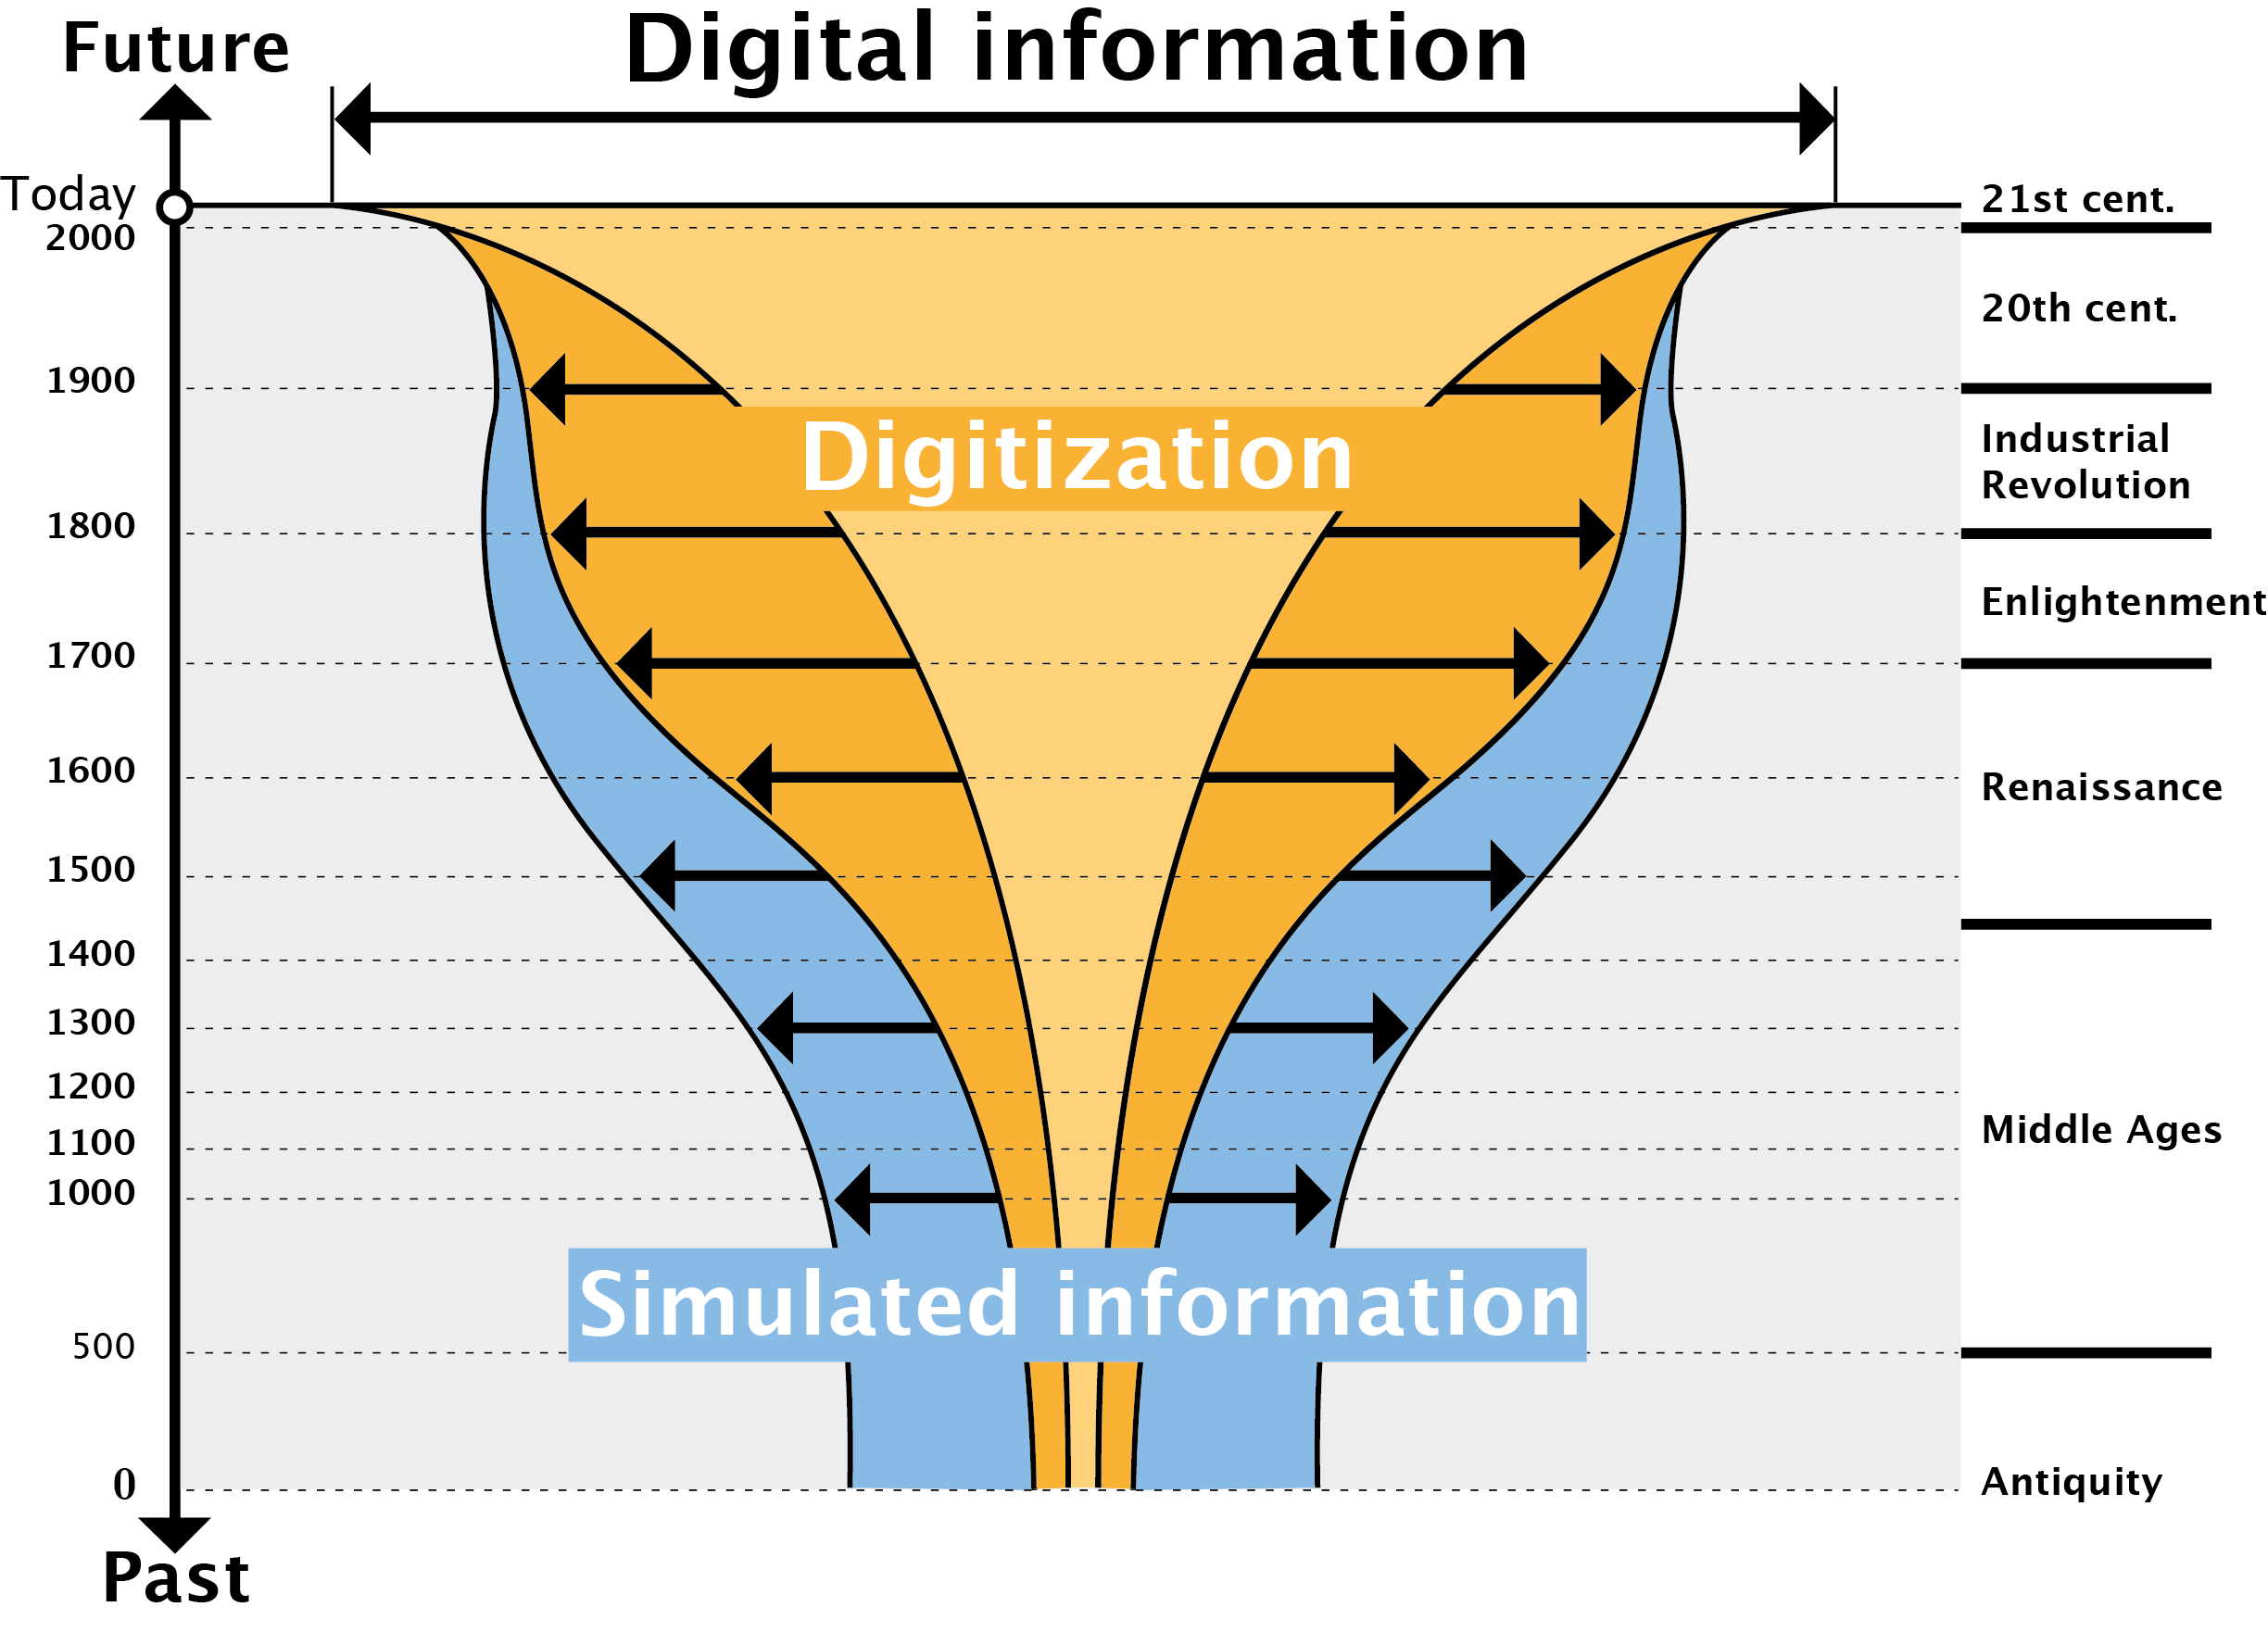
\includegraphics[width=\linewidth]{champignonKaplan.png}
%\end{sidecaption}
%\end{figure}

La classification automatique des données par l'ordinateur mais aussi la construction de modèles et leur simulation (au sens d'abord mathématique et parfois algorithmique du terme) apparaissent rapidement comme des enjeux pour la géographie. La simulation apparaît comme un outil de construction de connaissances absolument naturel et nécessaire pour confronter et construire les théories en rapport avec ces données \autocites{Kao1963, Hagerstrand1967b}. L'image de cette communauté interdisciplinaire agitant et confrontant ses problématiques méthodologiques, techniques, théoriques dans un but de progression commun, fait écho à des revendications plus récentes\Anote{jasss}. En réalité, cet esprit de partage tient d'une \enquote{volonté commune} qui apparaît quasiment avec l'apparition et la démocratisation des techniques de simulation. C'est ainsi que l'on trouve trace des efforts de cette communauté de chercheurs dans plusieurs ouvrages tels que \autocites{Borko1962,Beshers1965,Naylor1966,Dutton1971,Guetzkow1962,Guetzkow1972}.

Une citation d'un météorologiste du MIT, tout à fait remarquable par sa lucidité, anticipe ce qui sera le principal argument de l'emploi de la simulation en sciences humaines, à savoir un substitut à l'expérimentation.

\foreignblockquote{english}[\cite{Fleisher1965}]{I have argued that in the near future the social science will remain largely empirical and that simulation can serve as a device for making experiments \textbf{in vitro}. I think that this use is more important, at this time, than the massive making of models and that the principal contribution of simulation lies in the direction of intelligent, vivacious empiricism}

%Forrester1969 à ce sujet "In the social sciences failure to understand systems is often blamed on inadequate data... The barrier is deficiency in the existing theory of structure." \autocite[355]{Batty1976}

\subsection{Les conditions d'apparition de la simulation dans les différentes sciences sociales }
\label{sec:apparition_simu_science_sociales}

\subsubsection{Bref rappel autour des définitions de modèles et de simulations}
\label{ssec:rapell_termes_generiques}

Nous apportons ici une petite digression afin de préciser quelle acception de la simulation nous souhaitons mettre en oeuvre dans notre thèse.

\paragraph{Définitions générales du terme \enquote{modèle}}

\textcite{Varenne2013} ont entrepris une classification de la richesse historique des termes de modèle et de simulation.

La première définition généraliste et aussi la plus couramment rencontrée dans la littérature est probablement celle de \textcite{Minsky1965} établie en 1965 : \enquote{ Pour un observateur B, un objet A* est un modèle d’un objet A, dans la mesure où B peut utiliser A* pour répondre à des questions qui l’intéressent au sujet de A } \autocites{Varenne2008}[15]{Varenne2013b}

A partir de cette définition très formelle, \textcite{Varenne2008} relève dans une analyse plus moderne du terme les cinq points suivants :
\begin{enumerate}
  \item Le modèle n'est pas nécessairement une représentation.
  \item Le modèle doit son existence à l'existence d'un observateur subjectif, et d'un questionnement lui aussi subjectif.
  \item Le modèle est un objet qui a une vie propre, une existence autonome.
  \item L'existence du modèle est justifiée par l'existence d'une \enquote{fonction de facilitation}.
  \item Cette caractérisation minimale permet l'établissement d'une typologie.
\end{enumerate}

\textcite{Varenne2013b} propose dans des travaux plus récents d'associer à cette définition les travaux de Mary S. Morgan et Margaret Morrison qui replacent et caractérisent le rôle du modèle dans une enquête de connaissance par sa fonction de médiation (point 4 de la liste), une façon de faire écho à la problématique motivant la construction de modèles établis dans la définition de Minsky.

Un modèle est ainsi défini comme \enquote{\textit{un objet médiateur qui a pour fonction de faciliter une opération cognitive dans le cadre d'un questionnement orienté}, opération cognitive qui peut être de cognition pratique (manipulation, savoir-faire, apprentissage de gestes, de techniques, de conduites, etc.) ou théorique (récolte de données, formulation d'hypothèses, hypothèses de mécanismes théoriques, etc.)} \autocite[13-14]{Varenne2013b}

Les travaux actuels de \textcite{Varenne2008, Varenne2013b} dénombrent pas moins de cinq familles pour un total de vingt grandes fonctions, ce qui permet de situer efficacement la ou les problématiques - rien n’empêche les fonctions de se recouper - qui motivent la construction d'un modèle.

Nous verrons dans la section \ref{ssec:revol_modele} que les géographes modélisateurs ont mis dans leur définition davantage l'accent sur le rôle et les résultats attendus des modèles, plutôt que sur ces aspects formels.

\paragraph{Définition générale du terme \enquote{simulation}}

Le terme \enquote{simulation}, tout comme le terme \enquote{modèle}, est porteur d'une polysémie\Anote{polysemie_simu} qui remonte aux alentours de l'accélération de sa diffusion en 1960, mais nous retenons ici simplement les acceptions qui concernent la simulation computationnelle.

Bien que la simulation apparaisse sous sa première forme computationnelle dans la technique de Monte-Carlo et les travaux de Stan Ulman, John Von Neumann, Nicholas Metropolis \autocites{Eckhardt1987, Metropolis1987}, il faut attendre les années 1960 et les avancées techniques nécessaires pour que son utilisation semble utile au plus grand nombre. L'historienne en économie \textcite{Morgan2004} estime que le mot se diffuse vraiment dans la communauté interdisciplinaire, et en économie, aux alentours de 1960. Elle souligne le rôle central de Martin Shubik, un des pères de la théorie des jeux\Anote{shubik_jeux} dans la construction de ce débat\Anote{shubick_sympo} autour de la notion, comme celui qui a servi à la fois d'intermédiaire important dans la rencontre entre les différents acteurs de l'économie expérimentale et de l'informatique, mais aussi comme celui tout aussi important de prospecteur au travers des vastes études bibliographiques qu'il a réalisées sur le sujet \autocites{Shubik1960a, Shubik1972,Morgan2004}.

Par la suite d'autres conférences et ouvrages vont proposer de délimiter, toujours dans une construction interdisciplinaire, cet objet \enquote{simulation}, comme on peut le voir dans \autocites{Guetzkow1962, Borko1962, Guetzkow1972, Dutton1971}. La simulation computationnelle est rapidement reconnue par les disciplines en sciences sociales ou les sciences du comportement comme un outil important pour la construction et l'extension de théories (\textit{theory-building} ou \textit{model-building} selon la fonction définie pour le modèle), de par sa capacité à manipuler certes des symboles mathématiques, mais aussi des symboles de plus haut niveau d'abstraction, propre à l'établissement de règle \autocite[924-925]{Clarkson1960}. Dans notre étude, les modèles de simulation seront évoqués dans leurs dimensions avant tout numérique ou algorithmique (dirigés par des règles) \autocite[36-38]{Varenne2013b}.

\subsubsection{La simulation vue comme laboratoire virtuel d'expérimentation, une analogie ancienne}
\label{ssec:labo_virtuelle}

Parmi la vingtaine de fonctions épistémiques recensées par \textcite[14-23]{Varenne2013b} motivant la construction de modèles de simulation, la caractéristique la plus souvent exprimée pour l'époque en sciences sociales est sûrement cette capacité à pouvoir \enquote{expérimenter} sur les modèles en mobilisant des processus et des interactions sélectionnés et animés dans le cadre d'une dynamique, d'un temps mimant celui des systèmes cibles\Anote{varenne_temps}, et cela même dans des conditions difficiles caractérisées par l'absence ou l'inconsistance des données, les expérimentations réelles impossibles ou difficiles, etc., mais pas seulement car la simulation de modèles a aussi vocation à simplifier certaines simulations physiques coûteuses, ou trop limitées dans l'expression de nouvelles hypothèses. Ce lien entre simulation et expérimentation, complexe du fait de la relation entretenue entre le modèle et la réalité, est aussi ancien que la technique elle-même, Von Neumann affirmant dès le départ sa volonté de remplacer par des simulations sur ordinateur certaines techniques coûteuses de simulation physique \autocite[15]{Winsberg2013}.

Régulièrement employée dans la littérature, cette fonction d’expérimentation\Anote{laboVirtuel} revient également sous la forme de \enquote{laboratoire virtuel}, un terme qui prend selon les époques des teintes légèrement différentes, et cela quelles que soient les techniques sous-jacentes de support à la simulation des modèles.

Cette analogie ancienne entre simulation et laboratoire virtuel est illustrative d'une réalité dont on aurait bien du mal à nier l'existence tant celle ci est persistante dans cette littérature. Parfois le terme est invoqué directement, parfois il est implicite au discours présenté. Pour ne citer que quelques auteurs pionniers\Anote{legende_carnegie} dans l'historique de la notion, les premiers ouvrages collectifs en simulation et science sociale de \textcite{Borko1962, Guetzkow1962, Guetzkow1972}\Anote{ouvrage_1962}; les rapports et états de l'art des instituts scientifiques militaires américains \autocite{Harman1961}, et les travaux de Herbert Simon et Alan Newell \autocite{Newell1961}; et de façon plus localisé, en économie avec \textcite[915]{Shubik1960b}, en psychologie sociale avec \textcite{Abelson1968}\Anote{boudon_abelson}, le météorologue \textcite{Fleisher1965}, le couple d'Anthropologues/sociologues du comportement \textcite{Gullahorn1965}, l'archéologue anthropologue et informaticien \textcite{Doran1970}, la physicienne biostatisticienne et démographe \textcite{Sheps1971}, l'informaticien \textcite[3-4]{Forrester1971}, l'économiste informaticien \textcite{Naylor1966}, le professeur de science régionale \textcite[271]{Harris1966}, l'urbaniste \textcite[295]{Batty1976} sans oublier plus récemment \textcite{Epstein1996}, l'écologue \textcite{Grimm2006}, et encore sûrement bien d'autres auteurs. Une longue liste qui témoigne de l'intérêt pour cet outil bien au delà d'un simple critère de démarcation disciplinaire, technique, ou encore temporel; une hypothèse que nous allons développer par la suite.

\subsubsection{Un engouement pour la simulation qui touche l'ensemble des sciences sociales}
\label{ssec:engouement_sciencesociale}

Cet engouement pour la simulation de modèles touche toutes les sciences sociales ou presque. Nous dressons dans les paragraphes qui suivent une brève énumération des travaux qui en témoignent pour la période 1950-1970.

Suite au mouvement Cybernétique, à la convergence des travaux sur l'intelligence artificielle et les sciences cognitives, les premiers travaux qui visent la démonstration de la faisabilité de la simulation dans les sciences sociales viennent de Newell, Shaw, et Simon à la fin des années 1950 \autocite{Gullahorn1965}\Anote{gulahorn}. A ces travaux s'ajoutent ceux, en psychologie linguistique de l'équipe gravitant autour de \textcite[280-416]{Borko1962}, en psychologie des comportements sociaux de \textcite{Hovland1960}, d'\textcites{Abelson1961, Abelson1968} ou du couple \textcite{Gullahorn1965a} qui utilisent la simulation de modèles pour formuler, vérifier des théories sur la psychologie des individus et les modalités de leurs interactions avec les autres dans diverses situations\Anote{homonculus}, ce que \textcite{Ostrom1988} appellera \textit{a posteriori} les \foreignquote{english}{complex human processes}.

%La formation d’ingénieur de Coleman l’amène à prendre comme modèle un physicien : « My real hero is not Isaac Newton, but James Clerk Maxwell. He took Newtonian theory and developped from it a theory of gases, the Maxwell-Boltzmann distribution law of molecular velocities. I was fascinated by Maxwell because he was also concerned with the micro-macro problem. He had a very simple and neat theoretical framework of dimensionless molecules of any gas acting according to the law of motion, each with a certain mass and velocity. And from this he constructed a theory of gas. » (Coleman dans Swedberg, 1990, pp. 55-56).
\medskip
En \textbf{sociologie}, la simulation émerge dans les années 1960-1970 selon \textcites[50]{Manzo2005}[16]{Manzo2007}, sous l'impulsion de pionniers dans la sociologie mathématique comme \textcites{Boudon1967, Gremy1971} en France\Anote{gremy}\Anote{boudon}, ou James Samuel Coleman aux Etats-Unis\Anote{columbia_coleman}.

Coleman travaille sur des simulations liées à ses recherches sur l'éducation au début des années 1960 aux États-Unis, dont il a déjà publié des travaux dans l'ouvrage interdisciplinaire de \textcite{Guetzkow1962} en 1962, et qu'il publie ensuite \autocite{Coleman1965} dans une des premières revues abordant la méthode de simulation en sociologie, un numéro spécial des \textit{Archives Européennes de Sociologie} introduit par \textcite{Boudon1965} en 1965. Dans ce  numéro figure également une des premières publications de la simulation de diffusion d'\textcite{Hagerstrand1965} utilisant la technique de Monte-Carlo, un modèle qui recoupe les préoccupations du vaste courant interdisciplinaire dit des \textit{Social Network Analysis} (SNA) \autocite{Bernard2005}, qui touche tout autant aux structures de parenté (voir le paragraphe suivant pour des références en Anthropologie), qu'à la géographie (Hägerstrand à Lünd), ou à la sociométrie (modèle du sociologue mathématicien \textcite{Coleman1957}, mais également modèle de \textcite{Rapoport1961}, un biomathématicien de Chicago et cofondateur avec Boulding, Gerard et Von Bertalanffy de la société pour l'étude des systèmes généraux, ou GST)\Anote{lund_croisee}. Du point de vue français, outre l'analyse de Boudon sur ce sujet dans le numéro spécial de 1965, on trouve également une revue de ces mêmes avancées en simulation du côté de la sociologie politique (qui recoupe la psychologie sociale américaine), un état de l'art réalisé par \textcite{Padioleau1969} dans la \textit{Revue française de Sociologie} en 1969.

\medskip

En \textbf{archéologie}\Anote{retrospective_archeo}, dans la très claire rétrospective historique faite par \textcite{Lock2003} en 2003 sur l'histoire de l'archéologie computationelle, l'auteur s'attache à bien identifier au moins deux sinon trois époques aux méthodologies et aux outils différents. En adoptant une posture un peu simplificatrice, on peut donc affirmer que si l'archéologie d'avant 1960 se base principalement sur la récolte de données empiriques et la mise en exergue de \textit{pattern} dans ces mêmes données pour générer la plupart de ces explications, une rupture dans la discipline se dessine dès les années 1960-70 avec l'avénement d'un courant archéologique proclamant une \foreignquote{english}{New Archeology} (ou \textit{processualism}). Rejettant un empirisme beaucoup trop subjectif, celle-ci vante le retour à la seule \enquote{ Méthode Scientifique } pour générer des explications.

Si la critique de \textcite{Binford1962} cristallise pour beaucoup cette rupture, 1967-1968 est également considéré comme une période particulièrement importante pour la structuration de ce courant dans la discipline. Des comptes-rendus \autocites{Cowgill1967, Whallon1972} et plusieurs publications phares, y compris en France\Anote{gardin} avec les colloques de Marseille et les travaux de Jean-Claude Gardin \autocites{Gardin1971, Dallas2015}, viennent souligner l'émergence progressive dans les années 1960-70 de nouveaux outils\Anote{caa}\Anote{retrospective_caa}, à la fois computationnels comme les statistiques\Anote{wilcock_stat} ou la simulation \autocite{Clarke1968}, ou plus conceptuels avec l'ancrage de la \foreignquote{english}{New Archeology} dans la pensée systémique \autocites{Clarke1968, Flannery1968, Binford1968}\Anote{archeo_systemique}. Des avancées qui fournissent un véritable support à ce changement des pratiques dans la discipline.

%\autocite{Binford1983}
Si \textcite{Binford1968,Binford1972} représentent le point de vue américain, \textcite{Clarke1968} présente en Angleterre et à la même période (il est édité en 1968 par Binford) un point de vue un peu différent sur la \textit{New-Archeology}. Clarke est en effet sous l'influence des idées animant le campus de Cambridge, un haut lieu de changement ayant déjà accueilli une autre révolution, celle de la \textit{New Geography}\Anote{archeo_stat}. C'est dans cet environnement que Clarke publie en 1968 un premier livre \textit{Analytical Archeology} qui démontre le potentiel que pourrait avoir les statistiques spatiales, les modèles et la simulation stochastique en archéologie \autocites{Clarke1968, Clarke1972, Gardin1970}. Il est accompagné dans ses travaux par l'expertise, la volonté et les intuitions pionnières\Anote{doran_intuition} de \textcite{Doran1970} qui écrit également avec Hodson en 1975 l'ouvrage devenu référence \textit{Mathematics and Computers in Archaeology} \autocite{Doran1975} faisant état des travaux utilisant les toutes dernières techniques computationelles à la fois en traitement de données, et en simulation (Chaîne de Markov, Monte-Carlo, langage pour la simulation Dynamo, GPSS, etc.)

Ce militantisme semble recevoir un écho positif tout au long des années 1970, et certains auteurs comme \textcite[38]{Whallon1972} n'hésitent pas à définir\Anote{whallon_simulation} la simulation comme un prolongement naturel à la pratique existante de construction des modèles. Cette mise en oeuvre de programmes pionniers se poursuit avec une diversification dans les usages jusqu'au début des années 80 et constitue une première phase d'appréhension de la simulation, plus qu'une adoption massive par la discipline \autocite{Lake2013}.

% VOir aussi Mathematics and Computers in Archaeology doran 1975, partie sur la simulation cf http://books.google.fr/books?id=ZAPvXcnz0kkC&pg=PA369&lpg=PA369&dq=The+computer+in+archaeology:+A+critical+survey+whallon&source=bl&ots=6et-F8jHab&sig=gQWgTIHRuO2ICqMJtrRdGovo9gs&hl=fr&sa=X&ei=OskxU5W5Nen20gW0_4DIDA&ved=0CGUQ6AEwBQ#v=onepage&q=whallon&f=false

%\autocite{Clarke1987}

A la croisée de plusieurs disciplines en sociologie, anthropologie et géographie on trouve les modèles de variation de population, ou modèles démographiques dont les hypothèses sont amenées à varier selon des facteurs biologiques, économiques, spatiaux faisant souvent appel à une dynamique des interactions humaines impossibles à expérimenter dans la réalité\Anote{sheps}. Dans cette branche se côtoient donc, macro-simulation, micro-simulation et modèles analytiques hérités des premiers démographes mathématiciens, comme le plus connu d'entre eux, Lotka dont les premières publications sur le sujet datent de 1907 \autocite[355]{Veron2009}.

%%FIXE CLEMENTINE : c’est intéressant, que la plupart des travaux pionniers que tu cites  apparaissent dans les urban studies.  Est-ce que c’est la ville qui est si complexe ou une dépendance au chemin des méthodes dans les champs d’études ? ou parce que urban studies est particulièrement interdisciplianaire que ça a dépasser les barrières des affiliations disciplinaires ?

C'est autour de l'économiste et - on l'oublie souvent - également ingénieur constructeur de machines analogiques Guy H. Orcutt \autocite{Watts1991} et les équipes de l'\foreignquote{english}{Urban Institute} que sont développés \autocite{Orcutt1978} plusieurs modèles pionniers de micro-simulation comme RIM (1969), TRIM (1973), ainsi que DYNASIM\Anote{plateforme_dynasim} entre 1969 et 1975 \autocites{Orcutt1957, Orcutt1960, Orcutt1976}. Pionnier d'une longue série de modèles de micro-simulation qui s'étend jusqu'à aujourd'hui \autocites{Merz1991, Merz1994}, ce concept va aussi inspirer différents modèles dynamiques en démographie avec les travaux de \textcite{Perrin1964}, \textcite{Sheps1971}, et \textcite{Ridley1966} avec REPSIM aux États-Unis, \textcite{Hyrenius1964} en Suède, \textcite{Horvitz1971} avec POPSIM, ou encore SOCSIM basé sur les travaux en anthropologie de \textcite{Gilbert1966}, qui viennent compléter efficacement les modèles analytiques inspirés des travaux de Lotka \autocite{Sheps1971}, père entre autres de la démographie mathématique moderne. On retient également l'inscription du pionnier \textcite{Sakoda1949} dans les développements des travaux sur la famille \autocite{Potter1966}, qui utilise le langage informatique DYSTAL qu'il a développé spécifiquement pour la simulation en science sociale \autocites{Sakoda1965, Lee1995}. Coïncidence de l'histoire, ou inspiration commune, Hägerstrand apportera de façon parallèle en géographie et dans la même décennie \autocites{Hagerstrand1952, Hagerstrand1967a}, une vision micro similaire, à cela près qu'elle y ajoute un ancrage spatial des individus.

\medskip

Dans le cas de l'\textbf{anthropologie}, qui partage un tronc commun avec nombre de problématiques en archéologie et en psychologie, on retiendra le manuel édité par \textcite{Hymes1965} retranscrivant une conférence de 1962. Celui-ci contient deux articles importants pour la discipline, celui de \textcite{Gullahorn1965} et celui complémentaire de \textcite{Hays1965}. L'intégration de la simulation dans l'arsenal méthodologique prend part selon \textcite[274]{Bentley2009} d'un mouvement ayant pour objectif de mieux comprendre les contraintes sociales et culturelles dans les processus démographiques en général. Dans ce cadre par exemple de l'étude de la parenté ou \foreignquote{english}{kinship}, l'application de la simulation donne lieu à plusieurs expériences pionnières \autocites{Dyke1973, Dyke1981, Ruggles1993} en simulation comme celle de \textcite{Kunstadter1963}, mais aussi de \textcite{Gilbert1966}. Cet engouement continuera dans les années 1970 \autocite{Read1999} avec des simulations mettant en œuvre des processus stochastiques dynamiques comme par exemple dans les travaux de \textcite{Howell1978} et \textcite{Thomas1973}.

%\autocite{Costopoulos2007} . %Antony Wallace également, levy strauss 1955: les mathématiques de l'homme...

%En utilisant la simulation non pas comme un solveur d'équation mais en utilisant la puissance des opérateurs symboliques à sa disposition pour la mise en temporalités de systèmes d'interaction dans des sociétés passées, Doran décrit une vision de la simulation qui n'est pas sans rapeller le multi-agent d'aujourd'hui. Une conception de la simulation reprise et concrétisée par DH Thomas en 1972.\footnote{La discussion sur  \href{www.jiscmail.ac.uk/cgi-bin/webadmin?A2=ind04\&L=simsoc\&F=\&S=\&P=39083} {@SimSOC}}


% http://books.google.fr/books?id=G8sA95bz5pwC&pg=PA143&lpg=PA143&dq=%22Social+Physics%22+stewart+cybernetics&source=bl&ots=FsOC2mqHvr&sig=cS914G7pelGvgG6bG32fKsmWWPc&hl=fr&sa=X&ei=yTRAU5m7OIOH0AXwtYEY&ved=0CDsQ6AEwAQ#v=onepage&q=%22Social%20Physics%22%20stewart%20cybernetics&f=false
% "Social Physics" stewart cybernetics
% http://www.eoht.info/page/Princeton+Department+of+Social+Physics
% http://books.google.fr/books?id=F84mS2nnjWsC&pg=PA105&lpg=PA105&dq=geographer+reino+ajo&source=bl&ots=buVSBElr7Y&sig=_NXU0Py2goM2c6fVi1To3dUwqHQ&hl=fr&sa=X&ei=0DBAU_niJqrO0AWk44CwCw&ved=0CG8Q6AEwBw#v=onepage&q=geographer%20reino%20ajo&f=false
% http://www.persee.fr/web/revues/home/prescript/article/ingeo_0020-0093_1957_num_21_5_6491_t1_0223_0000_5#
% http://www.eoht.info/page/Social+physics
% Contributions to "social Physics" reino ajo
% Stewart, J.Q. "The Development of Social Physics"

\subsection{Les premiers modèles de simulation en géographie}
\label{sec:premier_modele_geo}

\subsubsection{Une \enquote{révolution quantitative} au cœur de multiples convergences}
\label{ssec:revol_quanti}

L'apparition et la diffusion de ces techniques quantitatives n'est pas le résultat d'une convergence unique, mais bien d'une succession de moments dont la fréquence et l'étalement temporel est difficile à cerner et empêche sur ce sujet toute exhaustivité.

On retiendra toutefois plusieurs grands facteurs, à la fois généraux, et d'autres plus spécifiques à la géographie, dont certains qui peuvent paraître étonnamment antinomiques. Une convergence qui s'illustre dans la richesse et la diversité des transformations qui touchent la discipline géographique entre 1950 et 1970, un constat déjà établi par bien d'autres auteurs \autocite{Varenne2014}.

%[28-29]Claval2003
%http://books.google.fr/books?id=s5xjIsejTjkC&pg=PA28&lpg=PA28&dq=h%C3%A4gerstrand+positivism&source=bl&ots=FrIMA95glO&sig=9Knqs1cLfJJefcc30qwsIMDzW-s&hl=fr&sa=X&ei=UMVDU86hJ-mS1AWPmIDoCw&ved=0CC4Q6AEwADgK#v=onepage&q=h%C3%A4gerstrand%20positivism&f=false

\paragraph{L'influence de l'école néo-positiviste}

Le néo-positivisme, néo-empirisme, positivisme logique selon les étiquettes, est un mouvement philosophique important, sinon peut-être le plus important, entre les deux guerres. Ce cercle dont on trouve les premières traces autour de 1908 à Vienne, est organisé autour de grands débats, dont la caractéristique est d'être fréquentée par un grand nombre d'intellectuels, issus de plusieurs disciplines. Tout au long de son évolution caractérisée par différentes phases (avec une apogée durant la troisième phase entre 1928-1934), de multiples courants d'opinions \textcite[126]{Ouelbani2006} vont être amenés à se côtoyer, du fait des débats internes, mais aussi des critiques extérieures au cercle. C'est donc à ce titre que \textcite[11]{Ouelbani2006}, préfère parler de \enquote{programme néo-positiviste}\Anote{ouelbani_positivisme} plutôt que d'un réel courant unifié.

Inspirés des sciences naturelles, et plus particulièrement d'une observation des sciences physiques et mathématiques, les tenants du programme néo-positiviste sont motivés par l'unification des sciences et pensent l'application d'un tel programme incontournable pour fonder des sciences sociales véritablement \enquote{scientifiques} \autocite[1-20]{Ouelbani2006}.

Les positivistes logiques ont ceci de particulier qu'ils raisonnent sur des démonstrations logiques encapsulant les énoncés observationnels décrits dans une logique formelle qu'ils veulent non ambiguë. Entre empirisme et logicisme, ce programme réductionniste\Anote{carnap} fait porter toute la connaissance sur l'expérience; ce qui mène avec l'aide de l'analyse logique et mathématique à l'élimination de toute métaphysique, et de toute structure a priori (anti-kantien) dans la construction des énoncés d'observation. Ainsi l'inférence déductive se fait seulement sur des énoncés d'observations qui sont \textit{a posteriori} tout à fait justifiables et donc mobilisables dans celles-ci seulement s'ils sont cohérents.

Selon le géographe épistémologue Olivier Orain\Anote{cour_orain}, \textcite{Hacking1989} a très bien saisi ce qui fait les axes communs des différentes relectures du terme positivisme.

\blockquote[{\cite[82]{Hacking1989}}]{Le positivisme peut se définir par quelques idées forces. \begin{enumerate*}[label=(\arabic*)] \item L’importance accordée à la vérification (ou à une variante comme la falsification) : une proposition n’a de sens que si l’on peut, d’une quelconque manière, établir sa vérité ou sa fausseté. \item La priorité accordée à l’observation : ce que nous pouvons voir, toucher ou sentir fournit, sauf pour les mathématiques, la matière ou le fondement le plus appréciable de la connaissance. \item L’opposition à la cause : dans la nature, on ne trouve pas de causalité dépassant ou surpassant la constance avec laquelle des événements d’un certain type sont suivis par des événements d’un autre type. \item Le rôle mineur joué par l’explication : expliquer peut contribuer à organiser des phénomènes mais le pourquoi reste sans réponse. On peut seulement remarquer que le phénomène se produit régulièrement de telle ou telle manière. \item Opposition aux entités théoriques : les positivistes ont tendance à être non réalistes parce qu’ils limitent la réalité à ce qui est observable mais aussi parce qu’ils s’opposent à la causalité et se méfient des explications. Leur rejet de la causalité les fait douter de l’existence des électrons simplement parce que ces derniers ont une action causale. Ils soutiennent qu’il s’agit là seulement de régularités constantes entre phénomènes. \item L’opposition à la métaphysique est finalement le dénominateur commun entre les points (1) à (5) ci-dessus. Propositions invérifiables, entités inobservables, causes, explications profondes, tout cela, dit le positiviste, est objet de métaphysique et doit être abandonné.\end{enumerate*}}

Une parenté qui dans le cas du programme néo-positiviste est difficile à isoler tant l'acceptation par les proches (comme Popper) ou membres du programme (certains préféreront même le terme empirisme logique) est amenée à varier. Pour en savoir plus sur ce sujet, on pourra se référer à cette classification proposée par \textcite[81-86]{Hacking1989}.

L'apogée du groupe à Vienne est de courte durée, avec les pressions du régime nazi et l'annexion de l'Autriche, le groupe est dissous. De nombreux acteurs du mouvement sont alors contraints à l'exil et nombreux sont ceux qui vont aux États-Unis. A ce moment-là, ce programme philosophique est alors quasiment inconnu des philosophes pragmatistes américains, mais paradoxalement il va trouver un très bon accueil sur ce nouveau territoire.

C'est sur cette philosophie pragmatique depuis longtemps installée (Peirce, Dewey) que vient se greffer ce nouveau programme, jusqu'à finalement quasiment l'éclipser. Un transfert que l'on n'imagine pas totalement unilatéral, et il est presque évident que le discours originel viennois tire largement profit d'une philosophie pragmatiste compatible dans ses fondements \footnote{ Ainsi selon \textcite[149]{Ouelbani2006} Carnap aurait été rassuré en 1935, date de son arrivée aux Etats-Unis, \enquote{ [...] de trouver une ambiance philosophique différente,en ce sens que les jeunes philosophes étaient intéréssés par des méthodes scientifiques et logiques}}. C'est ce que \textcite[123]{Wilson1995} affirme en disant que les pragmatistes \foreignquote{english}{[...] had created the conditions in which logical positivism and other analytic philosophies could flourish and ultimately displace them as the dominant voice in mid-century philosophical debates} mais aussi les conditions de son dépassement \foreignquote{english}{Pragmatism, then, not only created the conditions in which logical positivism and analytic philosophy could flourish in the United States, it also contained the seeds of the postanalytic philosophies that have attempted to move beyond [...] }. Ce programme va se diffuser à la fois sur les bancs des universités, mais aussi via les grands instituts scientifiques après-guerre qui font publicité de cette science \foreignquote{english}{mainstream}, organisée aux Etats-Unis autour de l'ordinateur.

La RAND fait partie de ces instituts fondés après-guerre qui approchent dès 1947 les sciences sociales \autocite{Rand106} et n'hésitent pas à mettre en avant par la suite les stars de la philosophie positiviste de l'époque comme Reichenbach \autocite[384-385]{Barnes2011} .

\paragraph{L'apparition de mouvements interdisciplinaires fédérateurs}

L'apparition de grands mouvements de convergence interdisciplinaires et leur intérêt pour l'application de nouveaux concepts et techniques aux sciences sociales, dont certains prennent par la suite la forme de paradigme du fait de leur portée d'application : Cybernétique de Wiener, \textit{projet} de la \foreignquote{english}{General System Theory} de Bertalanffy \autocite[9]{Pouvreau2013} s'organisent autour de grandes structures de recherches comme le MIT, la RAND, qui favorisent les collaborations par la mise en place d'équipes de travail pluridisciplinaires.

Parmi les ramifications directes de ces coopérations, on citera par exemple la \foreignquote{english}{social physics} de \textcite{Stewart1947}. Du fait des liens développés à l'université de Pennsylvanie, lieu de ses études et siège de la fondation de la science régionale d'Isard en 1954, Stewart sera amené avec sa rencontre avec Warntz, un géographe atypique qui plonge très tôt dans l'interdisciplinarité, à publier dans la revue \textit{Regional Sciences} \autocite{Stewart1958}.

Les retombées de ces interactions sur la géographie sont importantes\Anote{systemique_sousjacente}, et fournissent tout autant 
\begin{enumerate}[label=(\alph*)] \item des concepts généraux en correspondances avec les débats qui animent l'ensemble des sciences (sensibilités aux conditions initiales, équifinalité, bifurcation et catastrophe, boîte noire, rétro-causalité, hiérarchie d'emboîtement, etc.), \item un catalogue d'isomorphismes\Anote{isomorphismes} supplémentaires dont la correspondance reste à évaluer dans notre discipline \autocite{Wilson1969}, \item  une méthodologie et une typologie des modèles tirés de la recherche opérationnelle \autocite{Ackoff1962}\Anote{or_bertalanffy} et largement revendiqués par les géographes dans la décennie 1960-70, un constat tiré de la lecture d'états de l'art \autocite{Kohn1970}, ou d'ouvrages phares sur le sujet comme ceux de \textcites{Berry1964a, Haggett1965}, \item la découverte d'une science mathématique des systèmes dynamiques en correspondance avec ces nouveaux concepts, accessibles soit par un vocabulaire graphique opérationnalisable (DYNAMO, STELLA) \autocite{Forrester1961}, soit par des langages de programmation tout à fait traditionnels \autocite[304-305]{Batty1976} ! \end{enumerate}

On citera parmi les pionniers d'une exploration volontaire de cette convergence en géographie, \textcite{Haggett1965} en 1965, \textcite{Chorley1962} avec la géomorphologie en 1962 , \textcite{Berry1964a} avec les villes en 1964.

\paragraph{Les influences des \enquote{passeurs de modèles}}

Ces influences se sont réalisées à l'échelle internationale par Torsten Hägerstrand, Edgar Kant\Anote{footnote_kant}, Christaller et Lösch \autocite[119]{Berry1970}, ou dans un cadre plus national avec le travail de traduction ou de mise à disposition de textes originaux par les économistes et géographes Lösh, et Isard.

\paragraph{La conjoncture politique favorable}
% tous de chicago ?
L'impact de la conjoncture politique et l'importance de grands \textit{Think-Tank} comme la RAND, et du MIT qui remobilisent en sortie de guerre des armées d'ingénieurs alors désoeuvrés sur des missions plus scientifiques. On soulignera à la même période le rôle joué chez les géographes de Chicago \autocite{Harris1979}, Edward Ullmann \autocites{Ullman1941, Harris1977, Glick1988}, Chauncy Harris \autocite{Harris1945, Lichtenberger2005} et Edward Ackerman \autocites{Ackerman1958, Ackerman1963} dans la transformation institutionnelle de la géographie, dont la qualité en tant que corps de métier a pu être remarquée en temps de guerre. Cela se traduit sur la durée par un financement de la marine (\textit{Office Of Naval Research}), qui profite aussi de la nouvelle \textit{Regional Science} fondée par Isard. On trouvera plus d'informations sur ces inter-relations entre instituts après-guerre et leur impact sur l'établissement d'une géographie quantitative dans les publications de \textcites{Barnes2006a, Barnes2008}.

\subsubsection{D'une révolution quantitative à une révolution des modèles}
\label{ssec:revol_modele}

De cette \enquote{révolution quantitative} aux origines on le voit multiples, certains auteurs préfèrent ne retenir qu'une certaine essence de cette volonté nomothétique. Cette \enquote{révolution des modèles} comme préfèrent en parler \textcite{Wilson1970, Varenne2014} fait ici écho à cette déferlante de modèles qui apparaissent dans la décennie 1960-1970, et dont on trouve un recensement quasi exhaustif dans plusieurs ouvrages de référence \autocite{Haggett1965,Chorley1967}.

Une fois révélée cette profusion d'approches sous-jacentes à l'emploi, parfois confus, d'un même terme, s'ensuit chez les géographes une tentative de classification, de définition de cette pratique de modélisation. Il en ressort des typologies, l'évocation de divers substrats ( analogique, iconique, symbolique ) la plupart du temps empruntés dans les ouvrages de spécialistes alors disponibles. Ainsi, les deux sources d'inspirations de \textcites[106]{Berry1963}{Haggett1965} sont à ce moment-là des références issues d'un rapprochement avec la Recherche Opérationnelle (RO)\Anote{RO_collecte}, une discipline pionnière dont le développement après-guerre oeuvre pour l'application et la diffusion de méthodes numériques en vue de résoudre des problèmes extrêmement diversifiés. On retiendra des auteurs comme \textcite{Ackoff1962} (déjà cité par Ackerman en 1958) ou \textcite{Kemeny1962}

% détails typologies ?
\paragraph{Une autre définition des modèles et de la modélisation}
\label{p:autre_def_modele}

Alors que dans les faits beaucoup de choses ont changé sur le plan des pratiques, des techniques, des institutions, la référence à des définitions datant de 1965 reste après les années 1990 tout à fait acceptable \autocites{Dastes2001b, Antony2013}[295]{Bailly1995} et sert encore comme base de travail solide pour établir de nouvelles réflexions \autocite{Brunet2000}.

Comme nous l'indique \textcite{Haggett1965}, le modèle est pour les géographes avant tout un construit. En s'appuyant sur la typologie et la réflexion d'Ackoff, il définit ainsi dans \textit{l'analyse spatiale en géographie humaine} : \enquote{En construisant un modèle (\textit{model building}), on crée une représentation idéalisée de la réalité afin de faire apparaître certaines de ses propriétés } \autocite[30]{Haggett1965}.

% Brunet2000 définit également le modèle comme "processus de recherche" p28

A la différence de la définition donnée par Varenne\Anote{varenne_modele} et inspirée de Minsky (section \ref{ssec:rapell_termes_generiques}), celle de Haggett en 1965 met l'accent sur l'activité même de modélisation. Ce faisant, ce n'est plus tant la fonction définitive du modèle qui est mise en exergue ( \enquote{le pourquoi} motivant la sélection des propriétés saillantes) mais sa dimension en tant que construit.

Pour \textcite[36]{Langlois2005}, \enquote{le terme de \textit{modélisation} désigne à la fois l'activité pour produire un modèle et le résultat de cette activité.} Le concept de modélisation est donc \enquote{[...] plus large que celui de modèle, car il recouvre l'activité humaine qui aboutit au modèle achevé, alors que le modèle est un objet (concret ou abstrait), volontairement dépouillé de l'activité qui l'a créé}.

%modélisation = diachrnoqiue, temp long
%synchronique = extraction modele; temps court

L'activité de modélisation est donc un processus qui s'inscrit dans un temps long (diachronique), alors que le modèle peut être vu comme le résultat d'une extraction correspondant à un instantané de cette activité (synchronique). Ainsi de l'ensemble des choix qui ont constitué sa formation, le modèle ne porte plus après extraction qu'une histoire partielle de sa construction. Dans ce processus, toute opération cognitive qui n'est pas explicitement relatée est alors perdue dans cette compression d'informations.

%%FIXME CLEMENTINE : ça me fait penser à un article de Drogoul et al, 2003 : ou clairement, la modélisation est du temps long ET du collectif puisqu’il y a 3 rôles pour 3 modèles : thématique, conptuel, implémenté.

Un processus qui n'est pas limité à la seule construction de modèle de simulation et s'applique à la construction de n'importe quel modèle, comme le présente très bien \textcite[32-33]{Haggett1965} lorsqu'il évoque les deux voies possibles de construction de modèles théoriques. Dans la \textbf{première méthode}, que l'on pourrait qualifier de complexification progressive, \enquote{[...] le chercheur aborde \enquote{furtivement} un problème; il pose d'abord des postulats très simples et introduit peu à peu des complications, en se rapprochant toujours davantage de la réalité. Ainsi procède Thünen (1875) dans le modèle d'utilisation du sol qu'il présente dans son livre \textit{Der Isolierte Staat} (chap. 6, section 2) [...]}; une méthode qui autorise la divergence, le retour en arrière sur les hypothèses. Si au départ Thünen \enquote{[...] dans cet \enquote{Etat isolé} [...] suppose d'abord l'existence d'une seule ville, d'une plaine uniforme horizontale, d'un seul moyen de transport, et d'autres faits tout aussi simples[...]}, celui-ci \enquote{[...] brouille ensuite cette image en réintroduisant les objets mêmes qu'il avait tout d'abord supposés inactifs : sol de nature différente, marchés entre lesquels on peut choisir, moyens de transports divers.} La \textbf{seconde méthode}, symétrique, \enquote{[...] consiste à transformer la réalité par une série de généralisations simplificatrices}, qui permet comme dans le modèle de Taffe et Morrill (voir la description faite par \textcite[93-96]{Haggett1965}) de généraliser sur une base d'observations empiriques un certain nombre d'étapes stylisées qui interviennent dans le développement des voies de communication au Ghana.

%FIXME INTRODUIRE LE PASSAGE DU MODELE A LA SIMULATION DE MODELE, ET FAIRE UNE TRANSITION CORRECTE AVEC LA PARTIE D'APRES
Quant aux modalités guidant cette incrémentalité, celles-ci restent au demeurant très mystérieuses, et semblent plus relever au premier abord d'un art \autocites{Tocher1963, Axelrod1997} que d'une pratique véritablement rationalisée.

Le substrat de référence qui nous intéresse pour supporter les modèles est évidemment l'ordinateur. Or, si on se réfère au compte rendu réalisé par \textcite{Haggett1969} en 1969, celui-ci nous indique qu'à cette période l'ordinateur intervient dans au moins quatre usages qui font écho aux méthodes modernes considérées comme nécessaires selon \textcite{Claval1977} à l'évolution  de la géographie : (1) statistiques multivariées, (2) surfaces de tendances, (3) graphismes, (4) simulation.

Si l'on se réfère à la grille de fonctions établie par \textcite{Varenne2014}, celui-ci classe les modèles de cette époque comme étant en grande partie des modèles d'analyses de données ou des modèles théoriques à visée explicative. Sur cette base, il faut pour être exhaustif prendre en compte les modèles à visée prédictive pour l'aide à la décision, même si cela fait plus référence aux travaux réalisés dans le cadre des grands programmes de planification de la RAND, où les géographes mobilisés sont plus soumis aux directives d'ingénieurs que de chercheurs.

%Spécificité de l'objet d'étude "Le spatial et le temporel", objet d'étude des géographes
% FIXME : TRAVAILLER LE RACCROCHEMENT ENTRE LES DEUX
%Partant de la grille proposé par Varenne \autocite{Varenne2013x} il est possible de proposer un positionnement du modèle tel qu'on l'emploi le plus souvent aujourd'hui en géographie humaine quantitative; et de préciser le substrat sur lequel nous greffons différentes fonctions de médiations.

Afin d'illustrer l'importance de l'outil \enquote{modèles de simulation} dans la construction géographique théorique, et à condition d'accepter un découpage flou, on identifie deux grands moments innovants pour l'outil simulation en géographie, moments qui se juxtaposent partiellement dans l'espace et dans le temps.

D'une part; il y a l'apparition et la rencontre au début des années 1960 de deux pôles académiques innovants avec d'un côté les universitaires américains et suédois, et d'autre part il y a cette montée en puissance simultanée des instituts de planning aux USA, pilotés par des \textit{Think-Tanks} comme la \textit{RAND corportation}, qui commandent la construction de plusieurs modèles de simulations urbains entre 1959 et 1968 \autocite[307]{Batty1976}.

\paragraph{La rencontre entre les pionniers américains et suédois}

Ce premier moment prend appui sur les fondements de ce que l'on appelle aujourd'hui \enquote{la révolution quantitative}, notamment du fait du caractère international et multi-site de cette contestation. \textcite{Gould2004} proposenr toutefois de s'attarder en particulier sur deux premiers foyers importants dans cette \enquote{révolte}. Le premier socle se situe dans quelques universités \autocite{Gould2004} parmi lesquelles Washington (Seattle), Iowa (Iowa) et NorthWestern (Chicago); le deuxième socle est en Suède avec l'université de Lund; une liste à laquelle il faudra ajouter par la suite Cambridge, Bristol et Madingley \autocite{Haggett1989}, épicentres de la diffusion anglaise \autocites{Whitehand1970} qui va dans un troisième temps propulser sur le devant de la scène les \textit{terrible twins} Chorley et Haggett que l'on ne présente plus.

C'est à l'université de Iowa et de Washington, sous la direction de Edward Ullmann et William Garrison\Anote{premier_ordinateur}, qu'à la fin des années 1950 se forme un groupe d'étudiants qui va marquer le renouveau de la géographie. L'innovation des thématiques abordées dans les publications, mais aussi des formations proposées vont de pair avec l’entraînement mutuel qui anime cette équipe de jeunes doctorants formés à l'interdisciplinarité. Brian Berry, William Bunge, Richard Morrill, Duane Marble, Waldo Tobler, etc.; bientôt rejoints par Torsten Hägerstrand sont ainsi parmi les premiers à mettre en pratique les techniques computationnelles les plus récentes\Anote{dynamique_pionnier}.

Le déplacement de Torsten Hägerstrand de l'université de Lund aux Etats-Unis mérite une attention particulière, tant son impact sera important sur la discipline. Deux années après sa première publication en anglais en 1957, Hägerstrand est aussitôt repéré et invité par Garrison en 1959 à présenter ses travaux novateurs à une période, rappelons le, où la géographie est encore majoritairement idiographique en Angleterre mais aussi aux Etats-Unis. La rencontre a lieu à Washington dans un séminaire intitulé \foreignquote{english}{simulation modelling of the diffusion of innovation}. Réalisées à la main lors de sa venue à Washington\Anote{barnes_ibm}, les premières simulations Monte-Carlo\Anote{hagerstrand_mc} impressionnent les disciples de Garrisson, notamment Morrill \autocite[120]{Unwin1992}, qui à la suite de cette expérience va partir plusieurs mois en Suède \autocite{Morril2005}, ce qui lui inspirera d'autres développements s'appuyant sur cette technique, avec une application notamment sur le ghetto de Seattle \autocite{Marble1972}.

Il est difficile de savoir si les travaux de simulation pionniers de l'économiste Guy H. Orcutt \autocites{Orcutt1957, Orcutt1960} (niveau micro, Monte-Carlo, voir section \ref{ssec:crise_mutation}) ont déjà percolé jusqu'aux oreilles de Garrison, déjà bien renseigné par ailleurs sur le plan de la recherche en économie par sa proximité avec Isard, ou si ces travaux usant de Monte-Carlo paraissent totalement novateurs à ce moment-là; reste que la démonstration de ce couplage efficace entre nouvelles techniques et nouvelles questions impressionne \autocite[120]{Unwin1992}, et fait dire à \textcite{Morril2005} et \textcite{Gould1970} tout l'impact que ces travaux ont eu sur ses contemporains.

Il faudra attendre quelques années pour que les simulations soient effectives; en Suède, probablement en langage machine sur le premier ordinateur de l'université de Lund nommé SMIL (\foreignquote{sweden}{Siffermaskinen i Lund} ou \foreignquote{english}{The Number Machine in Lund}) construit sous la principale influence de Carl-Erik Froberg et que l'on sait utilisé très rapidement par Hägerstrand\Anote{hagerstrand_lund}, un ami d'enfance de Froberg; et en Fortran\Anote{marble_hagerstrand} aux Etats-Unis par le duo Pitts et Marble \autocites{Morril2005, Marble1972, Pitts1963}. Le modèle est publié en 1965 en Europe dans le journal en trois langues \textit{Archives Européennes de Sociologie} (European Journal of Sociology) \autocite{Hagerstrand1965}, et en 1967 \autocite{Hagerstrand1967a} aux États-Unis le plus connu sur cette technique.

%%FIXME Ajouter témoignage de DUANE au dessus en rapport avec les deux dates !

Suite à cette publication de 1967, la spatialisation des processus de diffusion décrits par Hägerstrand vont inspirer le développement d'autres travaux en géographie et dans d'autres disciplines où le thème est déjà abordé au niveau macro, en sociologie avec la diffusion d'innovation chez Coleman \autocite{Coleman1957}, en épidémiologie \autocite{Cliff1981} où la diffusion de processus a déjà été étudiée (Bailey 1957, Bartlett 1960) \autocite{Pitts1963, Morrill1968}, mais aussi dans les études de migration motivées en géographie par les travaux de Morrill, Pitts et Marble, dérivé de \autocite{Wolpert1965}, mais aussi de ceux de Cavalli-Sforza en 1962.

\paragraph{L'influence de l'économie, entre travaux universitaires et commandes des instituts étatiques}

D'autres techniques de simulation, à la fois déterministes et probabilistes, sont également introduites à cette période en géographie, comme les méthodes de programmation linéaires ou l'utilisation de chaînes de Markov \autocites{Marble1964, Clark1965, Whitelegg1976}. La percolation de ces techniques se fait en premier lieu via des mathématiciens vers les économistes \autocite{Samuelson1952} et son introduction chez les géographes est à chercher ensuite du côté des ouvrages pionniers d'Isard \autocites{Isard1958, Isard1960} et son disciple Stevens \autocite{Stevens1958}.

Compte tenu de la proximité entre Isard, Ullman, Ackerman et Garrisson \autocite{Barnes2004} qui vont initier par la suite plusieurs générations de géographes en s'appuyant sur des modèles d'économie spatiale dans le cadre des \textit{regional sciences} \autocite[120]{Unwin1992}, il est normal de retrouver ces techniques opérationnelles innovantes \footnote{ \foreigntextquote{english}[Unwin1992, 120]{Garrisson argued that the use of algebraic notation and linear programming methods enable problems of location structure to be given an operational character, and that problems couched in such terms \enquote{\textit{display the price interdependencess associated with the location system in a manner which was not possible before}}}} assez rapidement dans les publications des géographes américains, comme cette première application assez connue de Garrison et Marts en 1958 \autocite{Garrison1958}.

%http://www.aag.org/cs/membership/tributes_memorials/gl/golledge_reginald

\paragraph{L'écho des premiers travaux individu centrés}

Un peu plus tard, et dans la continuité des travaux déjà réalisés dans les simulations mettant en œuvre des discrétisations de l'espace comme celles d'Hägerstrand, ce sont les automates cellulaires qui apparaissent dans la continuité des travaux de Von Neumann sur la théorie des jeux. 

On connaît bien évidemment les travaux isolés, pionniers et souvent oubliés \autocites{Hegselmann2012, Aydinonat2007} du psychologue James Minoru Sakoda \autocite{Sakoda1949} (implémenté sur ordinateur en \autocite{Sakoda1971}), ceux plus connus de de Schelling (1969, 1971, 1978) \autocite{Ganguly2003} qui dans une interview dit ne pas avoir connu ces même travaux de Sakoda \autocite{Aydinonat2005}, et enfin Axelrod(1984). Mais le premier à évoquer spécifiquement la technique d'automate cellulaire pour l'analyse de phénomènes socio économiques serait de l'avis général l'économiste américain Peter S. Albin dans son livre \textit{The Analysis of Complex Socioeconomic Systems} \textcites{Smith1976, Ganguly2003}.  En géographie, il y a les nombreux travaux inspirés du modèle de simulation d'Hägerstrand (qui ne porte pas encore le nom d'automates cellulaires), puis le travail de Tobler \autocites{Tobler1970b, Tobler1979}\Anote{tobler_michigan} et celui de Couclelis \autocite{Couclelis1985}. On trouve pour la géographie une description plus détaillée de cette technologie dans les travaux de \textcite{Louail2010}.

%L'introduction de la dimension spatiale et temporelle est importante ici ...

%Du coté des géographes, les pionniers Suédois de l'école de Lund et Américains de l'école de Washington saisissent dès 1960-70 cette opportunité d'accélérer la résolution de modèles explicatifs déjà éprouvés avec du papier et du crayon en usant des tout premiers ordinateurs; car c'est à cette époque que sont justement développés les premiers langages informatiques génériques, et même si ceux ci sont d'abord réservés à quelques élites pionnières ayant accès à du matériel et aux multi-compétences adaptés, très vite de jeunes chercheurs formés à l'interdisciplinarité vont permettre la diffusion de ce savoir faire (Morril, Marble, Tobler, etc.).

Cet engouement constaté pour la simulation de modèles dans les sciences sociales est suivi peu après par une crise de confiance dont il existe peu de témoignages directs. Il faut le remettre en perspective dans un historique propre à chaque discipline, sur le plan spatial et temporel, ce qui rend extrêmement difficile la définition de ces contours. Plusieurs auteurs, la plupart du temps les pionniers, font toutefois l'état des difficultés rencontrées.

% Citer troizsch avec son schéma

\subsection{Une crise de confiance envers l'outil ?}
\label{sec:critiques_simulation}
\Anotecontent{starbuck_footnote}{Starbuck met l'effet de tassement des publications sur les trois dernières années sur le compte du nombre croissant de publications, impossibles à comptabiliser.}

Deux travaux de \textcite{Dutton1971} et \textcite{Starbuck1983} identifient un ralentissement des publications à partir de 1970. L'étude de 1971 est inédite, et consiste à éplucher et classer de façon exhaustive la littérature portant sur la simulation. Plus de 12000 publications en anglais pourront être classées, et plus de 2000 papiers seront identifiés traitant spécifiquement de la simulation en \foreignquote{english}{Human Behavior}. Si ce ralentissement dans la publication de simulations n'est pas forcément observable en 1969, date qui marque l'arrêt de l'étude\Anote{starbuck_footnote}, Starbuck constate par contre en 1983 la quasi-absence de nouvelles publications sur le sujet, voire pire, la remise au goût du jour de modèles de plus de 20 ans.

Une surprise qui finalement n'en est pas une, car dans l'étude de Starbuck en 1971, moins de la moitié des publications ne proposait aucun modèle implémenté, la plupart des études se bornant à une discussion méthodologique.

Pour appuyer et résumer ce constat assez terrible, Starbuck cite John McLeod, un scientifique pionnier qui travaille depuis plusieurs décennies dans des journaux dédiés à la simulation ( \textit{Simulation} créé en 1963 , et \textit{Simulation and gaming} en 1970):

\foreignblockquote{english}[\cite{Starbuck1983}]{According to  John McLeod who has been involved with Simulation magazine for two decades, one primary reason for the methodology's sorry state is that simulators have overstated its capabilities and so, subsequently, disapointed their audiences.}

\subsubsection{Les principales disciplines touchées en sciences sociales}
\label{ssec:disciplines_touches}

En \textbf{archéologie}, plusieurs témoignages \autocite[6-7]{Lake2013} font état d'une période de relative inactivité\Anote{temoignage_archeo_alden} qui démarre au début des années 1980. Après avoir cru pendant longtemps cette période comme \enquote{morte}, celle-ci est aujourd'hui caractérisée par \textcite{Lake2013} comme une période de maturation bénéfique, marquée par un changement de discours, car plusieurs modèles qui déboucheront sur des résultats importants sont développés durant les années 1980, et seulement publiés après 1990\Anote{temoignagne_lake}. \textcite{Lake2013} donne également plusieurs pistes pour expliquer les facteurs à l'origine de cette inactivité, dont une particulièrement intéressante dans le cas de Hodder, qui est amené à la fin des années 1970 à faire un volte-face vis-à-vis des espoirs qu'il avait mis dans l'outil simulation.

\foreignblockquote{english}[{\cite[7]{Lake2013}}]{In the introduction to his 1978 [...], Hodder expressed optimism about the utility of simulation in archaeology (Hodder 1978, p. viii), yet just four years later, in one of the founding works of postprocessual archaeology, he rejected the positivist inferential strategy and functionalism of the New Archaeology [...] (Hodder 1982). Ironically, the results of Hodder's own simulations (Hodder and Orton 1976) were a contributory factor in his volte-face because they revealed how the problem of equifinality could profoundly undermine attempts to quantitatively test hypotheses about settlement pattern and trade mechanisms}

Il est possible de trouver d'autres explications dans une revue de méthodes réalisée par \textcite{Doran1986}, qui pointe l'importance d'une démarche abductive associée à l'emploi de nouvelles méthodes \autocite{Doran1982} issues de l'intelligence artificielle (multi-acteur et systèmes experts) en archéologie.

\foreignblockquote{english}[\cite{Doran1986}]{Looking back at the decade, there is clear progress both in exploring new and in refining old models and methods. But there are all too few examples where a decisive contribution has been made to an archaeological problem of substance - comparable,say, with the benefits provided by the techniques of the physical sciences. Many reasons may be and have been given for this lack of archaeological payoff, prominent amongst them being inappropriate importation of formal techniques from other disciplines [...], a tendency by archaeologists to \enquote{go it alone} and redesign (inferior) methodological and theoretical \enquote{wheels}, and a tendency for formal tools simply to be misused. [...] Yet whatever the technical expertise which becomes available, formal models and the formal methods associated with them will not yield useful results unless archaeologists pose important and relevant questions. In terms of the interpretive framework given earlier, unless the explanatory models employed relate to or, better, are part of substantial archaeological theory, the whole interpretive exercise is sterile. Unfortunately, just what constitutes explanatory archaeological theory is a matter of some considerable controversy.[...] The time when the New Archaeology held the high ground (in American archaeology at least) are long gone. Now it is the surviving new archaeologists themselves who are on the defensive against a wave of criticism.}

A la problématique d'assimilation des techniques dont la complexification mathématique et conceptuelle courant des années 1970 ne cesse d'isoler les pionniers, vient donc se greffer la critique d'un mouvement \foreignquote{english}{post-processualist} critiquant la \textit{New Archeology} qui va constituer un véritable frein au développement de modèle. A une époque similaire, on trouve un mouvement équivalent en géographie, avec l'émergence d'une frange de géographes radicaux s'appuyant sur divers facteurs dont l'affaiblissement du dogme néo-positiviste et le revirement brutal de certains géographes (Harvey par exemple) pour critiquer les modèles (voir section \ref{ssec:transition_annee70}).

\medskip
Autre discipline, et même constat affiché par \textcite{Ostrom1988} en \textbf{psychologie sociale}. Alors qu'il revendique en 1988 l'importance de la simulation comme un \foreignquote{english}{third way system} pour faire de la science, il fait également un constat assez accablant sur la place aujourd'hui tenue par cette pratique de modélisation dans le courant \foreignquote{english}{mainstream} de la psychologie. Ainsi dit-il \footnote{ \foreignquote{english}{Despite the clear relevance of these models to  social psychology, the simulation approach had not caught the imagination of main stream social psychologists. Very few simulations had appeared in the core journals of the field prior to the publication of Abelson's chapter. […] At the time of Abelson's writing, simulation models had not made much contact with the dominant empirical pursuits of the field. } \autocite[382]{Ostrom1988}}, force est de constater le peu de retours rapportés par la communauté face aux manifestes des pionniers tels que \textcite{Gullahorn1965} ou \textcite{Abelson1968}

\medskip

En \textbf{anthropologie}, \textcite{Dyke1981} dresse de son côté un maigre bilan\Anote{dyke_bilan} et donne, malgré l'augmentation du nombre de publications sur ce sujet, quelques éléments d'explications pour justifier ce désengagement de l'outil dans sa discipline, parmi lesquels figurent un possible effet de mode exagérant les capacités réelles de la simulation et la problématique de la validation des modèles\Anote{dyke_validation}. 

\medskip
Enfin, en \textbf{sociologie} en France, le témoignage du sociologue Manzo, très investi dans la réflexion et la communauté multi-agents, est tout à fait révélateur de la place encore très minoritaire occupée par la simulation en sociologie, totalement absente de la littérature depuis 1965 :

\foreignblockquote{english}[\textit{Extrait tiré de la présentation de cette publication sur le \href{http://www.gemass.org/manzo/writing-agent-based-computational-modeling}{@site} du GEMASS.}]{During the last decade, research on/using agent-based computational modelling has spread impressively quickly. [...] My original motivation to submit a project for a special issue on agent-based modeling to the Revue Française de Sociologie was a simple fact: no French sociological journal seemed pay attention to the interest raised by this simulation method within the international community. In my opinion, this was somewhat paradoxical. Historically, leading figures of French sociology was far ahead of their time when, in the sixties and seventies, contributed to introduce the idea of generative models in sociology and suggested computer simulations as a promising tool to study this kind of models. To find a special issue devoted to simulation by a journal strongly related to the French sociological community, one has indeed to go back to that time, when Raymond Boudon edited in 1965 \enquote{Simulation in Sociology} for the Archives Européennes de Sociologie in which even pioneering, although ignored and forgotten, agent-based simulations ante litteram are presented (see Torsten Hägerstrand’s article). To fill this gap, I submitted my proposal to the Revue Française de Sociologie in 2011. The project was accepted in 2012 and the call for papers (in French and English) was sent out in April 2012.}

On trouve également un témoignage plus direct de ce phénomène dans les propos de \textcite{Gremy1971} :

\blockquote[\cite{Gremy1971}]{Après l'engouement suscité, entre 1960 et 1965, par les premières expériences simulées, l'emploi des techniques de simulation semble cependant avoir déçu les espoirs des sociologues; pourtant, ces techniques sont d'un usage courant en recherche opérationnelle depuis 1950 environ et paraissent donner entièrement satisfaction à leurs utilisateurs. Il nous semble que cette désaffection passagère des sociologues à l'égard de la simulation tient à un malentendu touchant le rôle que cette approche peut jouer dans l'étude des phénomènes sociaux. Certains pionniers de la simulation en sociologie ont espéré aboutir à la création d'une sorte de \enquote{macrosociologie expérimentale}; c'est sur cet espoir que s'est fondé le retentissement des premières applications de la simulation en sociologie et c'est probablement l'échec de cette tentative qui explique la désaffection observée à l'égard de la simulation. Notre propos est de montrer que \textit{la simulation ne constitue pas une approche expérimentale des faits sociaux} et que son emploi ne saurait conférer à la sociologie empirique le statut de science expérimentale, mais que l'intérêt majeur de la simulation est qu'\textit{elle met les ressources considérables de l'informatique au service de la réflexion théorique.}}

\subsubsection{Une mutation dans la construction des modèles en géographie ?}
\label{ssec:crise_mutation}

\begin{figure}[htbp]
\begin{sidecaption}[Photographie d'un mainframe IBM 7094]{Une image de la série 7094 pris dans la collection de photographies historiques sur le site \href{http://www-03.ibm.com/ibm/history/exhibits/mainframe/mainframe_album.html}{@IBM} }[fig:I_IBM]
  \centering
 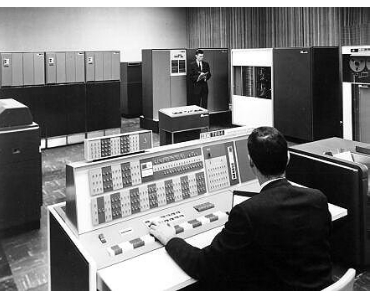
\includegraphics[width=.8\linewidth]{IBM7094.jpg}
  \end{sidecaption}
\end{figure}

Fruit des diverses influences citées auparavant, le cas de la géographie en particulier est traité un peu à part des autres disciplines en sciences humaines et sociales, car plus qu'une crise les années 1970-80 semblent -- une hypothèse à prendre toutefois avec prudence -- avant tout avoir constituées le socle fertile d'un renouvellement dans l'activité de modélisation, empruntant la voie de la mathématisation avec semble-t-il plus de facilité que d'autres sciences sociales. Une explication à chercher peut-être dans les fondements de la révolution quantitative, car pour \textcite{Gould1970} \foreignquote{english}{The intellectual revolution in geography since the middle and late fifties rests upon two main supporting pillars - men and machines.}

En parallèle du perfectionnement des machines et de leur puissance de calcul apparaissent des langages de programmation qui vont faciliter la construction et la diffusion des méthodes de simulation. Nous n'envisageons pas d'en faire un historique complet, mais nous en donnons un aperçu dans l'encadré \enquote{Les premiers langages de programmation}.

D'un point de vue technique \textcite{Haggett1969} cite comme véritable point de départ dans la discipline la démocratisation de l'accès à la ressource informatique après 1961, avec la diffusion d'une deuxième génération d'ordinateurs dans les grands centres de calcul, en partant notamment de la série IBM 7094, le \textit{Vogelback Computing Center}\Anote{vogelback_marble} ouvert en 1965 à Northwestern avec un CDC 3400 apparemment très vite complété avec la sortie du CDC 6400 (600 cartes perforées par minutes ! Une bonne occasion pour apprendre à utiliser correctement le matériel de perforation \autocite{Fisk2005}) sur lequel vont travailler des pionniers comme Duane F. Marble\Anote{marble_computer_historycdc}.

Des ordinateurs que l'on imagine beaucoup plus accessibles et performants que la précédente série IBM 604 et 650\Anote{tobler_650} \autocite[584]{Barnes2004b} à \textit{vacuum tube} utilisés au début des années 1960 à l'université de Washington\Anote{ibm604650} et Iowa, des précurseurs qui seront rapidement remplacés, par exemple par l'IBM 1620 enfin utilisable avec le langage Fortran I \autocite[66]{Berry2005}.

\pagebreak

\begin{testiv}{Les premiers langages de programmation}{Les premiers langages de programmation}

La période 1955-1965 est une période où la simulation est reconnue comme une méthode de résolution d'un certain nombre de problèmes difficilement tractables mathématiquement \autocites{Nance1993, Ackoff1961}. Des programmes de développement visant à mettre en place des modèles de représentation, de description nécessaire et facilitant la construction de simulations se multiplient. Deux classes de langages informatiques vont voir le jour durant cette période, et vont continuer à se développer et à s'influencer chacune de leur côté jusqu'à encore aujourd'hui. D'une part, des langages de plus haut niveau apparaissent avec pour vocation de se positionner comme une alternative plus expressive que l'assembleur. Dans cette optique le premier compilateur FORTRAN apparaît en 1957,  Algol en 1958, Cobol en 1959, et Lisp 1958. Ces langages et leurs successeurs sont d'usage assez générique et permettent de décrire correctement tous types de programmes. Toutefois à l'époque de leur apparition, ils sont d'accès relativement difficile pour une personne non initiée, ce qui nous amène au développement sur la même période d'une deuxième catégorie de langages informatiques, plus spécialisés dans la construction spécifique de modèle de simulation \autocite[239]{Naylor1966}.

A la même époque, des langages spécialisés dans l'expression des simulations apparaissent, et pour la plupart s'appuient et évoluent en parallèle des développements des langages classiques sur lesquels ils s'appuient. Ces SPL ( \foreignquote{english}{Simulation Programming Langages}) comme Simula en 1962 ou bien Dynamo en 1958 ont ceci d'intéressant qu'ils ont très largement accompagné les formidables avancées conceptuelles de cette époque et cela au travers des différentes disciplines. Ainsi; la première période 1955-1960 est marquée par la mise au point de GSP (\foreignquote{english}{General Simulation Program}) par Owen et Tocher \autocites{Tocher1960, Hollocks2008}. Celui-ci est considéré comme le tout premier langage mis au point pour faciliter la description de simulation sur ordinateur. Un effort que Tocher va accompagner d'une publication phare en 1963 dans le livre \foreignquote{english}{Art of Simulation} \autocite{Tocher1963} . Vient ensuite une autre génération de langage en 1960-1965 comme GPSS (\foreignquote{english}{General Purpose System Simulator}), Simscript (développé sous l'impulsion de la RAND corporation), et la première version du langage SIMULA, qui donnera naissance à la fin des années 1960 à Simula-67, un langage qui aura un impact dépassant largement la classe des SPL, et inspirera les créateurs des futurs langages objets comme Alan Kay, plus connu comme le créateur du premier langage objet SmallTalk. 
On trouve plus d'informations sur cette période spécifique abordée sous l'angle de l'ingénierie logicielle dans les publications de \textcites{Nance2013, Nance1993, Araten1992, Nance2002}.

%On trouve plus d'informations sur cette période spécifique abordée sous l'angle de l'ingénierie logicielle dans les publications de \textcites{Nance2013, Nance1993, Araten1992, Nance2002} et en consultant les \href{http://informs-sim.org/}{@archives} de la WSC (\textit{Winter Simulation Conference}). 

Cette dernière, si elle n'est pas la première à aborder cette thématique (le \textit{System Simulation Symposium} en 1957 selon Nance), est la première à vouloir pérenniser le débat à un niveau national \autocite{Nance2002}. Fondée en 1967 \autocites{Crain1992, Araten1992}, celle-ci jouit aujourd'hui d'une très large visibilité au niveau international, notamment car elle abrite les publications de pionniers et de membres importants pour la discipline simulation. On pourra citer par exemple Sargent et Balci, des pionniers dans la construction de la discipline de la \textit{Validation and Verification}, qui participent et publient régulièrement dans le cadre de cette conférence.

Les \textit{procedings} de la conférence WSC accueillent ces dernières années le récit d'un projet réunissant un grand nombre d'acteurs importants pour l'émergence de la simulation \autocite{Nance2013}. Une fondation créée pour cette occasion est chargée de la récolte des témoignages audio et vidéo, de leurs préservations et de leurs mises à disposition avec tous les documents initiaux fondateurs sur le \href{http://d.lib.ncsu.edu/computer-simulation/}{@ComputerSimulationArchive} hébergé par la \textit{North Carolina State University}.
\end{testiv}

En Grande Bretagne, en 1951 il y aurait eu 4 ordinateurs seulement. En plus des universités déjà pionnières (Edinburgh, Londres, Oxford, Cambridge) et sous l'impulsion du \textit{Flowers Report}, les universités s'équipent progressivement à partir du milieu des années 1960 suivant ce plan établi nationalement. On trouve un peu partout dans les universités\Anote{atlas} un motif assez similaire à celui de l'université de Bristol décrit par \textcite{Haggett1969}, c'est-à-dire une hiérarchie de machines qui va par ordre croissant de puissance de l'IBM 1620 et PDP 8 (Faculty level), l'Elliott 503 (University level), \textit{English Electric System} 4-75 (South West Regional Computer Centre). Viennent ensuite les machines des différents centres de traitements nationaux (plus souvent renouvelées) comme le \textit{SRC Atlas Computing Centre} de Chilton, le \textit{National Computing Centre} de Manchester, et bien d'autres centres plus petits, la plupart du temps accessibles à distance aux universitaires par divers terminaux. \textcite{Rhind1989} témoigne de la présence à l'université d'Edinburgh en 1967 d'une \textit{English Electric System KDF9} de puissance probablement similaire à celle évoquée par Haggett à Bristol. Depuis 1969 et jusqu'à 1973, soit un an à peine avant la commercialisation des tous premiers \textit{microcomputers}, \foreignquote{english}{The most sophisticated computing system in British universities was the NUMAC one, serving the whole of the universities of Newcastle and Durham: this IBM 360/67 had 1 Mb of main memory.}\Anote{numac} Un 360/65 est également installé la même année à l'\textit{University College} de Londres.

La mise en perspective de ces machines anglaises avec les travaux des géographes Ward et Weeb est intéressante. Ceux-ci se sont associés à l'informaticien Levison pour concevoir et exécuter des simulations spatiales de type Monte-Carlo pour étudier les théories de peuplement de la Polynésie, en utilisant l'ordinateur ATLAS, entre 1964 et 1971 \autocites{Montillier1974, Ward1973}. Cette expérience est régulièrement citée par \textcites{Gould1970, Gould1975} comme un autre des usages pionniers mêlant une discrétisation spatiale, un tirage Monte-Carlo, et une représentation des résultats sous forme de carte.

\foreignblockquote{english}[\cite{Gould1970}]{Handling space and time simultaneously is a difficult business, and simulation, for all its current detractors, often appears to offer the only feasible way out. [...] In an intriguing study of Polynesian drift voyaging, over 800000 items of data had to be stored in the computer’s memory before the Monte Carlo process could even begin [...] The model generated starting islands, and then simulated the drift voyages by drawing from probability distributions assigned to each five degree grid cell in the Pacific Ocean.}

\foreignblockquote{english}[\cite{Doran1974}]{ By use of computer techniques the authors have simulated an enormous number of voyages in the Pacific, over 100,000 drift voyages and about 8,000 guided voyages [...] Results of the various experiments are displayed on a series of maps showing probabilities of contact among islands, both by drift and by navigated voyages. An appendix reproduces eighty-four computer maps, each from a single experiment, which show the position of each vessel on each day of the many voyages. As many as 50,000 dots are shown on each map, providing an excellent visualization of the field covered by the experiment.}

%FIN ORTHOGRAPHE EMILIE

En Nouvelle-Zélande, Golledge nous indique que l'installation sur le territoire de la firme IBM semble précéder de peu la formation des pionniers \autocite[94]{Bailly2000} et au début des années 1960 l'université de Canterbury se porte acquéreur d'un flambant neuf IBM 1620 doté de 32K de mémoire.\Anote{ordinateur_actuel}

\Anotecontent{histoire_suede}{Une récolte de documents publique nationale a été organisé par le \textit{tekniskamuseet} de Suède, les textes sont disponibles à l'adresse internet suivante \href{http://www.tekniskamuseet.se/it-minnen}{@tekniskamuseet}}

En Suède\Anote{histoire_suede}, trois ordinateurs sont construits dans le courant des années 1950-1960 : SARA par la société Saab à Linköping, DASK à l'institut scientifique de Copenhague, et SMIL à l'université de Lund \autocite{Persson2007}. Carl Erik Frödberg, un ami d'enfance de Hägerstrand, fait partie avec Eric Stemme des consultants amenés à échanger sur le sol américain avec les leaders du domaine (Neumman, etc.) afin de démarrer le programme suédois.  SMIL est capable de compiler de l'Algol, et c'est probablement sur celui-là que Hägerstrand assisté de Frödberg a pu exécuter ses premiers programmes. En 1969, un Univac 1108 est acheté pour faire suite à SMIL \autocite[33-34]{Lindgren2008}.

En France, en 1955 il y a exactement six ordinateurs \autocite[3]{Armatte2008}, mais c'est seulement en 1970 que l'université Paris 1, centre de référence pour les géographes pionniers quantitativistes, se dote d'un ordinateur Philips et d'un terminal en contact avec le calculateur d'Orsay. Nous verrons plus en détail la relation historique des géographes aux centres de calcul dans la section \ref{sec:retourgeoHPCopenmole}.

Toutefois, on ne peut parler d'une véritable démocratisation de l'outil informatique chez les chercheurs qu'avec l'apparition dans les années 1974 aux États-Unis des premiers postes informatiques individuels \autocite[221]{Ceruzzi2000} et il faudra encore attendre le milieu des années 1980 pour que cette technologie se diffuse véritablement et touche le grand public.

A cette période, la mise en oeuvre de modèles de simulation est fortement limitée par des problématiques humaines et techniques \autocites{Haggett1969}[387]{Marble1972}, dont on peut constater dans les ouvrages interdisciplinaires vus dans la section précédente, qu'elle ne touche pas en réalité que la géographie \autocite{Guetzkow1972}.

C'est toutefois dans cette période où les compétences informatiques nécessaires à la programmation se font encore très rares, les langages de programmation multiples et peu stables, le matériel coûteux et peu disponible (nécessitant des opérateurs de saisie, temps d'utilisation partagé entre différentes disciplines, accessible seulement localement), que des packages de programmes sont peu à peu publiés et mis à disposition des chercheurs via les réseaux universitaires \autocite{Haggett1969}.

Au niveau de ces réseaux de diffusion de programmes, selon \textcite[20-21]{Greer1972} deux sont à noter : \textit{the State Geological Survey of University of Kansas (Computer Contributions)}  et \textit{ the Department of Geography of the University of Nottingham U.K. (Computer Applications in the Natural and Social Sciences)}. Au niveau des progiciels, \textcite[20-21]{Greer1972} identifie en 1972 trois pôles universitaires importants : Iowa \autocite{Wittick1968}, Northwestern \autocites{Marble1967, Marble1972b, Marble1972,Marble2010}, Michigan \autocite{Tobler1970c}\Anote{programme_trouver}. En effet, des pionniers comme Marble ou Tobler mettent à disposition dans le courant des années 1960 différentes routines informatiques en libre accès. \textcites[3]{Marble1967, Pitts1968} parlent de 150 routines développées jusqu'à 1967, et cela seulement à Northwestern dans le département de géographie. Le premier \textit{Statistical package for Social Science} pour les sciences sociales (ou \href{http://www.spss.com.hk/corpinfo/history.htm}{@SPSS}) date quant à lui de 1968 \autocite{Barnes2011}, alors que sort à la même date l'ouvrage \foreignquote{english}{best-of} de \textcite{Berry1968} \foreignquote{english}{Spatial Analysis: a Reader in Statistical Geography}, qui offre une vision d'ensemble des derniers développements statistiques et mathématiques.

En faisant régulièrement état de leurs avancements dans divers rapports ou publications\Anote{programmes}, les pionniers Marble, Morrill, Pitts et Bowlby \autocite{Pitts1963} qui se placent dans la continuité des premiers travaux relatifs aux processus de diffusion d'Hägerstrand \autocite{Hagerstrand1953, Hagerstrand1967a}, donnent ainsi à voir les efforts et les difficultés auxquelles la petite équipe doit faire face pour améliorer les programmes ou les adapter à des problématiques différentes.

Sur un tout autre front, celui du développement des \textit{Large Scale Models} \autocites[8]{Batty1976}, les universitaires géographes sont plus souvent cités comme spectateurs qu'acteurs \autocites[9]{Batty1994}[153]{Batty1989}, cela même si quelques universitaires arrivent à décrocher des contrats importants \autocite{Barnes2006a} pour des études plus pratiques, comme \textcite{Garrison1959}, notamment du fait que les objectifs poursuivis sont relativement différents, la planification et la prédiction prenant plus souvent le pas sur la curiosité et l'explication scientifique. Toutefois, et si l'on en croit \textcite{Haggett1969} la communauté universitaire semble attendre beaucoup des retombées de ces grands programmes, qui disposent de moyens humains et économiques importants pour développer des programmes et collecter des données. Cette crise, qui on l'a vu touche avant tout les instituts de planification américains couverts par la RAND, va fournir le terreau nécessaire à la transformation d'une discipline dont le rayonnement dans la communauté scientifique à l'international ne va aller qu'en s'amplifiant après 1970 (voir la carte \ref{fig:S_carte_wegener}).

\begin{figure}[htbp]
\begin{sidecaption}[Centres de recherches les plus actifs en modélisation urbaines à la fin des années 1980]{La carte des centres de recherches les plus actifs à la fin des années 1980, début des années 1990 selon \textcite{Wegener1994}}[fig:S_carte_wegener]
  \centering
 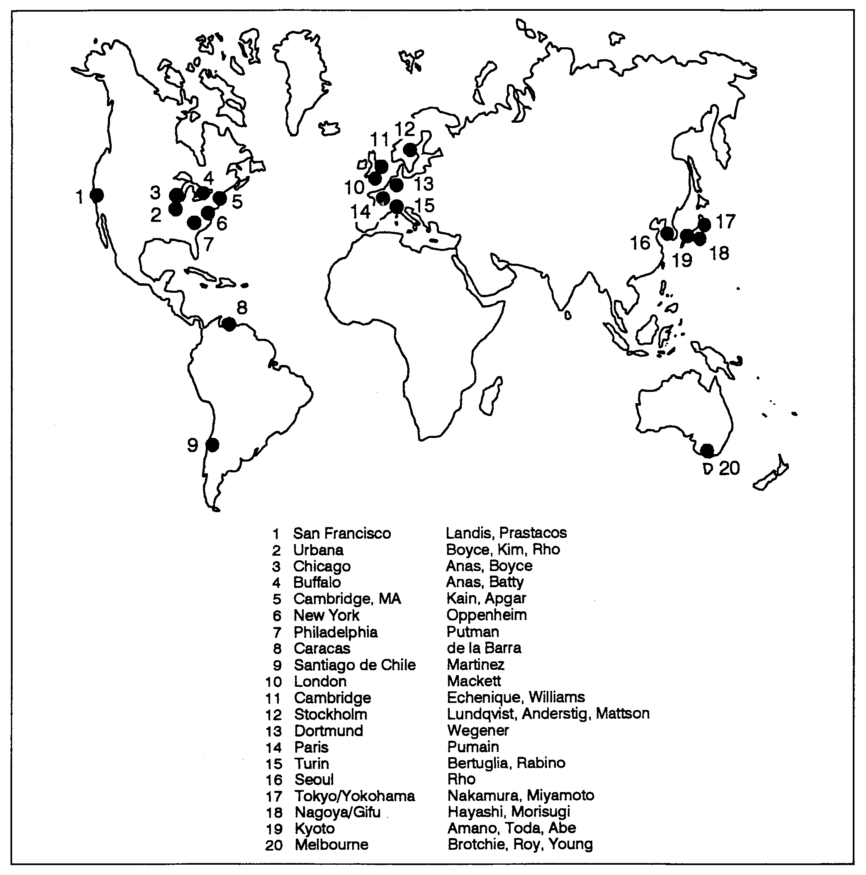
\includegraphics[width=.9\linewidth]{carte_wegener.png}
  \end{sidecaption}
\end{figure}

Si le requiem de \textcite{Lee1973} a bien eu un effet non négligeable sur la construction et la publication de tels modèles du coté des planificateurs \footnote{Seulement trois modèles seront publiés dans le même journal à la suite de cet article ...}, force est de constater que la construction de modèles de simulation pour la théorie urbaine ne disparaît pas dans cette période \autocite[11-12]{Batty1994}, et s'appuie au contraire sur l'apprentissage de ses échecs pour se réinventer dans les années qui suivent. A ce titre, \textcite{Harris1994} soulève dans une relecture très critique de l'article de Lee, l'ignorance ou la méconnaissance de l'auteur vis-à-vis des débats qui agitent déjà depuis plusieurs années la simulation de modèles urbains \autocites{Batty1971, Wilson1970, Orcutt1957, Harris1968}. Ce faisant, Harris accuse Lee d'enfoncer des portes ouvertes et de porter des accusations que certains jugeront par la suite prématurées vis-à-vis du préjudice subi, touchant à cœur une discipline d'à peine une décennie et encore en phase d'apprentissage. \autocite[p11]{Batty1994}.

Ce mouvement de modélisation doit faire face à l'expression de ces limitations pour se reconstruire, limitations dont on sait par avance qu'elles ne seront pas seulement levées par la seule amélioration des techniques.

D'une part l'emploi de théories trop simplistes, induit indirectement la nécessité d'un retour à une démarche inductive plus exploratoire \footnote{On notera par exemple le témoignage de \textcite{Boyce1988} lorsqu'il dit à propos des chercheurs engagés dans cette voie \foreignquote{english}{Some, including myself, turned to more empirically oriented research activities, perhaps in the hope of strengthening the foundation of future models}}, jusque là mise de coté.
%\hl{On peut ici aussi ajouter la référence aux différents articles de l'ouvrage anniversaire (20 ans apres model geography) Remodelling Geography de MacMillan en 1987}

D'autre part, si les universitaires américains semblent rater le coche de cette transformation, en Europe plusieurs écoles viennent à se former, et intègrent les défauts et les qualités de cette génération précédente de modèle. C'est le cas par exemple au Royaume-Uni où sont récupérés les modèles américains ayant donné de bons résultats, comme celui de Lowry \autocite{Lowry1964}, pour servir de base à de nouveaux travaux mettant en perspective l'influence ou les progrès d'autres courants disciplinaires en contact avec la géographie. Car une autre voie d'évolution possible pour les modèles vient des travaux existants réalisés dans d'autres disciplines universitaires ou dans le monde industriel. Ainsi différentes équipes de développement sont déjà bien identifiées dans la communauté des économistes comme \textcite{Orcutt1957} et son premier modèle micro \foreignquote{english}{bottom-up} développé à l'\textit{Urban Institute}, et l'apport de \textcite{Forrester1961,Forrester1969} sur l'optimisation industrielle, une des branches opérationnelles d'inspiration la plus directe du projet systémique au début des années 1960 \autocites{Cohen1961}[911]{Shubik1960b}. Ces deux exemples font dans leur implémentation dynamique alors écho aux travaux initiaux du géographe Hägerstrand, et poussent dans cette période de reconstruction toute une partie des géographes à réintégrer la dimension temporelle à des modèles d'optimisation statique en échec \autocite[p295]{Batty1976}.

%\pagebreak

\bigskip

% et Hagerstrand ?
\begin{testiv}{La diffusion de la micro-simulation}{}

La \enquote{micro-simulation} initiée par Orcutt, qui semble effectivement passer outre l'extinction annoncée par Lee en 1973, rencontre même un certain succès durant toutes les années 1970 comme en témoigne la mise en place de nombreux programmes nationaux au début des années 1980 \autocites{Merz1991, Merz1994, Baroni2007}. Comme l'indique également \textcite{Boman2005} en citant \textcite{Merz1991} : \foreignquote{english}{[...] 57 major dynamic and static microsimulation models had been developed and implemented between 1960 and 1990. They covered the following topics: wealth accumulation and distribution, labor force participation, pension reform, family formation, distributional effects of tax transfer policies, urban housing markets, distributional impact of energy policies, national health insurance, state unemployment insurance, land-use forecasting, residential energy demand, housing allowance, labor supply, shortening of working hours, distributional impacts of child allowance changes, market and non-market activities, shadow economy, effects of tax regulations on industrial firms, and more.}

Une réponse à cette survie peut être avancée dans le positionnement innovant d'Orcutt pour faire face aux résultats décevants des \textit{Large Scale Models} de son époque, opérant pour la plupart à un niveau macro et fournissant des résultats hautement agrégés difficiles à exploiter dans un cadre prédictif, et finalement peu représentatifs de la diversité des systèmes économiques \autocites{Birkin2012, Baroni2007}. Si les critiques de Lee peuvent pour la plupart être mobilisées pour critiquer les modèles issus de la micro-simulation (complexité des modèles, absence d'objectifs clairement posés, volume des données à mobiliser, complexité des calculs, coût de construction, absence de résultats, etc.), il n'en reste pas moins que la proposition d'Orcutt introduit avec une approche plus \textit{bottom-up} une dimension explicative absente jusque là. En répondant à l'observation de Lee sur l'absence d'extraction de connaissances micro quelque soit la complexité injectée dans les modèles macro, Orcutt ouvre d'une certaine façon la voie à des développements théoriques beaucoup plus riches que ne le permettaient à l'époque les seuls modèles macro, faisant ainsi de son modèle un instrument réceptacle idéal pour accueillir des éléments de complexification issues des sciences sociales \autocite[19]{Czajka1993}. Un travail pour \foreignquote{english}{consolidating past, present, and future research efforts of many individuals in varied areas of economics and sociology into one effective and meaningful model; an instrument for combining survey and theoretical results obtained on the micro-level into an all-embracing system useful for prediction, control, experimentation, and analysis on the aggregate level} \autocite[122]{Cohen1961}.

D'un autre coté, cette micro-simulation telle que déjà théorisée par Hägerstrand dans sa version spatiale ou par Orcutt dans sa version économique, va étonnamment et cela pendant plusieurs années rester un courant ayant peu d'impact sur le développement des modèles urbains en économie spatiale \autocite[5]{Sanders2006}, et cela malgré plusieurs appels d'un côté \autocite{Hagerstrand1970} ou de l'autre \autocite[5]{Isard1998}. De façon indépendante et dans un univers somme toute limité par de fortes contraintes techniques et financières, ces travaux vont toutefois dans leurs lentes et multiples convergences donner naissance autant à des modèles universitaires qu'à des programmes nationaux (DYNASIM et CORSIM pour Orcutt aux Etats-Unis, SVERIGE en Suède, etc.). Pour finir cette parenthèse sur la micro-simulation par une petite transgression temporelle, si peu de modèles existent encore dans les années 1990, plusieurs publications récentes font état d'un inversion de la tendance ces vingt dernières années \autocite{Lenormand2013}, avec une augmentation (et une diversification ? ) croissante des modèles, sûrement liée à des capacités de développements informatiques plus importants, tant du point de vue des données, que de la puissance d’exécution qui admet l'importance croissante du parallélisme, idéale pour simuler des entités individuelles. \autocites[5]{Sanders2006}{Lenormand2013}

\end{testiv}

D'autres écoles apparaissent dans le courant des années 1970, comme celle de \textcite{Wilson1970} dont l'émergence est considérée comme un des moments importants dans le renouveau des modèles urbains \autocite{Griffith2010}; mais également d'autres écoles comme celle de Peter Allen, qui s'appuient sur l'évolution des mathématiques et le transfert méticuleux de concepts observés en physique pour construire des modèles à la fois spatiaux et dynamiques capables de simuler de façon plus réaliste les interactions complexes intervenant dans la formation et l'évolution des villes \autocites[11]{Batty1976}{Batty2001}[27-28]{Pumain2003}\Anote{pumain_gain}.

La diffusion et la généralisation du \enquote{projet systémique} de Bertalanffy dans de multiples disciplines permettent aux géographes d'accéder à tous les outils conceptuels et surtout opérationnels \autocite{Forrester1969} nécessaires pour penser, modéliser et simuler les systèmes géographiques au travers de leurs interactions complexes, en intégrant dans leurs analyses cette hétérogénéité d'échelle caractéristique des objets géographiques, comme peut l'être par exemple la région.

Ainsi pour \textcite[11]{Batty1976}, de façon plus importante que tous les autres problèmes, c'est la révélation dans l'observation de cette richesse et de cette complexité d'interactions des facteurs causaux à l’œuvre dans l'évolution et la structuration des phénomènes urbains qui va le plus contribuer à la réévaluation des formes de modélisation. Révélé par Batty comme le problème de l'\textit{Observational Dilemna} \autocite[11,296]{Batty1976}\Anote{observational_dilemna}, celui-ci s'impose à la fois comme un constat faisant suite à cette première génération de modèle\Anote{problem_generation_model} et une conséquence de cette prise en compte nécessaire de la \enquote{dynamique} dans les futurs modèles de simulation\Anote{batty_dynamic}. Tout en restant critique sur les capacités de celui-ci, c'est le modèle de Forrester \textit{Urban Dynamics} \autocite{Forrester1969} qui cristallise selon \textcites{Batty2001, Batty2005b} le mieux cette transformation dans la façon de penser la construction et la validation des modèles de simulation urbains au début des années 1970\Anote{observational_validate}.

Nous aurons l'ocasion de revenir plus en détail sur cette décennie charnière (section \ref{ssec:transition_annee70}) en abordant tout à la fois le glissement progressif de la géographie dans une pensée systémique et son impact sur les écoles anglaises et françaises de modélisation (section \ref{sssec:progressive_systemique}), jusqu'à évoquer plus concrétement cette \enquote{problématique de la Validation} au travers des arguments croisés de Forrester et de Batty (section \ref{sssec:forrester_impact}).

\subsubsection{De fortes limitations techniques et méthodologiques}
\label{ssec:limitation_techniques_methodologiques}

Dans la lignée des témoignages de \textcite{Marble1972}\Anote{marble_validation}, les modèles spatiaux restent selon \textcite{Batty1976}\Anote{limitation_batty} encore très limités dans leur complexification, ou même leurs évaluations compte tenu des ordinateurs à disposition des géographes.

Malgré les apports heuristiques indéniables qui vont avec l'utilisation de l'outil, on retrouve l'expression de difficultés concernant le calibrage des modèles plus complexes chez de nombreux auteurs pionniers modélisateurs \autocites{Batty1976,Pumain1983b}[400]{Sanders1984}, notamment pour ce qui concerne le calibrage des modèles, souvent difficile pour ces modèles dynamiques non linéaires soumis à de telles fluctuations dans leurs comportements. Voici comment \autocite{Pumain1998a} résume les difficultés opérationnelles résultats de plusieurs années de travaux menés autour des modèles de simulation dynamiques non-linéaires opérant dans le cadre de la théorie de l'auto-organisation : \enquote{Les difficultés de calibrage, associées à la capacité élevée de bifurcation des modèles, ont été maintes fois décrites, de même que l’impossibilité de valider comme \enquote{meilleur ajustement} une configuration donnée de paramètres.}

Se pose alors la question suivante, l'incapacité à calibrer un modèle de simulation n'est-elle pas un problème qui limite de facto l'évolution en crédibilité de l'outil simulation ?

On perçoit pourtant très tôt chez certains géographes la nécessité d'optimiser cette étape, rendue improductive et dangereuse du fait de la non-linéarité des modèles \foreignquote{english}{The trial and error method of searching for best-parameter values by running the model exhaustively through a range of parameter values or combinations thereof represents a somewhat blunt approach to model calibration. [...] Moreoever, as each run of the model can be expensive or take a large amount of time, few applications have attempted to find systematically the optimum parameter values [...] Clearly, then, there is a need for the introduction of methodes suitable for calibrating intrinsically non-linear models of spatial interaction.} \autocite[155]{Batty1976}

Des méthodes basées sur des méta-heuristiques de type descente de gradient, ou \textit{hill-climbing} sont déjà utilisées par les géographes comme \textcite[159-160]{Batty1976} pour résoudre des problèmes d'optimisation utilisant les sorties de modèles. Toutefois ces méthodes sont encore trop souvent limitées à des modèles à 1 ou 2 paramètres, s'avèrent peu robustes face à des problèmes acceptant des minima locaux, et se limitent à l'optimisation de fonctions uniquement unimodales. Les équipes françaises se heurtent également à ces problématiques au début des années 1980, et ces nouveaux modèles \enquote{complexes} restent très difficiles à calibrer avec les moyens informatiques disponibles, même lorsque ceux-ci sont importants \autocites{Pumain1983b, Sanders1984}.

A cela vient s'ajouter une autre problématique. En effet, à l'inverse des pionniers géographes français qui manifestent très tôt la volonté d'une modélisation en confrontation avec l'empirie \autocites{Pumain1983,AMORAL1983}, \textcite{Openshaw1989} formule à la fin des années 1980 quelques critiques sérieuses à l'égard d'un mouvement de modélisation anglo-saxon qui se serait replié dans la production de modèles essentiellement mathématiques et théoriques\Anote{end_mathematical_area}. La prise en compte lucide de la complexité des systèmes urbains et de l'impossibilité d'en observer ou d'en recolter de façon simple la substance causale (\textit{observational dilemna}) ne doit pas masquer la nécessité d'une confrontation pratique avec les données, ne serait-ce que pour nourrir en retour les constructions théoriques. Si Batty en est bien conscient, ce n'est pas semble-t-il le cas de tout un courant de modélisateurs anglo-saxons à cette époque. \textcite{Openshaw1989} nous dit également que cette \enquote{problématique de la Validation} n'a pas toujours été abordée de façon concrète\Anote{openshaw_critique_math}, par le spectre d'outils ou de méthodes susceptibles d'être mis à disposition des modélisateurs. L'absence dans la littérature de logiciels, de codes sources, ou de réelle méthodologie pour la construction ou l'évaluation des modèles de simulation face aux données reste selon \textcite{Openshaw1989} un frein à toute adoption plus large de cette activité de modélisation. Comme le laisse aussi supposer le titre du chapitre 1 de \textcite{Batty1976} \textit{The art of urban modelling}, construire des modèles reste à cette période une activité dont \enquote{les rouages informatiques} sont bien gardés. %En france aussi

L'appel à l'utilisation de nouvelles méthodes pour l'exploration des modèles déjà lancé par \textcite{Batty1976} sera par la suite repris de façon implicite dans les travaux innovants menés par l'équipe de géographes de Leeds, principalement guidée par l'inventivité d'Openshaw \autocites{Openshaw1983, Openshaw1988, Diplock1996, Turton1998}. Celui-ci publie par exemple avec \textcite{Diplock1996} un des premiers articles sur les algorithmes génétiques utilisés pour estimer des paramètres de valeurs inconnus lors des calibrages de différents modèles spatiaux :

\foreignblockquote{english}[\cite{Diplock1996}]{The results demonstrate that even GA en ES can provide very good solutions for spatial interaction model calibration, albeit sometimes at the expense of considerable extra compute times. [...] It would also be worth considering the use of other forms of global optimization method; [....] As computer hardware becomes faster, the attraction of simple, relatively assumption-free, and highly robust approaches to global parameter estimation can only grow and allow the geographical model builder to worry less about the problems of parameter estimation and focus more on the task of model design.}

Remis en perspective de l'\textit{observational dilemna} de Batty, la dernière phrase d'Openshaw prend alors tout son sens. La possibilité d'une telle systématisation dans le calibrage des modèles permet au modélisateur de se concentrer sur le seul vrai débat censer rythmer la construction des modèles de simulation, à savoir la sélection et la justification des hypothèses que l'on veut intégrer dans la structure causale de nos modèles de simulation. Avec de tels outils s'appuyant sur des puissances de calcul intensives bien au-delà de ce que permet un micro-ordinateur, la dépendance des modélisateurs à la ressource informatique se renforce en réalité encore un peu plus dès lors qu'on considère la nécessité d'explorer les modèles, non plus lorsqu'ils sont terminés, mais dès que la première brique est posée.

Cette réponse plus méthodologique et technique à \enquote{la problématique de la Validation} sera discutée (section \ref{ssec:evaluation_construction}) à la fois dans ses implications épistémologiques (explorer ainsi les modèles de simulation est-il suffisant pour dire de ceux-ci qu'ils sont validés ?) mais également dans ses implications plus concrètes, dans le cadre d'une évolution des pratiques de modélisation au laboratoire Géographie-cités (partie 2 de la thèse).

\subsection{Synthèse}

%%FIXME PAGE REF DYKE

Il semblerait donc que la pratique de la simulation en sciences sociales se concentre ensuite dans les années 1980 sur de petites communautés de chercheurs, disposant de fortes compétences techniques initiales, qui vont continuer à travailler, à proposer des modèles et à acquérir de nouvelles techniques et méthodologies en parallèle d'un courant plus \textit{mainstream} intégrant seulement les nouvelles capacités offertes par les ordinateurs mais délaissant parfois l'aspect simulation. Dès les années 1980-1990, plusieurs chercheurs pionniers, comme Jim Doran \autocites{Doran1982, Doran1985, Doran1986, Doran1986b}, réapparaissent conjointement avec l’avènement d'une nouvelle innovation dans les techniques de simulation en partie dérivée des progrès en intelligence distribuée; un retour dont on verra qu'il se fait cette fois-ci avec plus de succès.

En s'appuyant sur ces livres interdisciplinaires déjà cités de multiples fois \autocite{Dutton1971,Guetzkow1962, Guetzkow1972} et sur ce qui a été dit dans ce chapitre, voici une liste forcément non exhaustive d'arguments évoqués par les auteurs pour justifier de cette baisse effective dans la confiance envers l'utilisation des modèles de simulations : \textbf{(1)} l'effet de mode initial qui exagère largement les capacités de l'outil pour expliquer ou prédire \textbf{(2)} les effets négatifs d'un rattachement volontaire ou involonaire à l'idéologie néo-positiviste, un programme épistémologique vivement critiqué durant les années 1970 dans plusieurs disciplines des sciences sociales, \textbf{(3)} la non-adéquation entre la richesse d'expression des théories sociales et la concision/réduction mathématique, \textbf{(4)} l'absence de standard de validation prenant en compte le cadre thématique, voire l'absence complète de validation, \textbf{(5)} la non-adéquation avec un courant théorique \textit{mainstream} réfractaire, \textbf{(6)} les capacités encore limitées des ordinateurs de l'époque, pour le stockage des données, pour l'exécution des programmes, pour l'exécution des analyses sur les modèles, et pour les réplications nécessaires à la validation, \textbf{(7)} l'ignorance ou la difficulté à mettre en oeuvre les techniques adéquates, va de pair avec le manque de formation/compétences pour ces nouveaux outils dans la discipline, et rend difficile l'exploitation et la construction des modèles, \textbf{(8)} l'existence de parcours et de stratégies de publications scientifiques non adaptés pour ce nouvel objet de recherche qui limite sa diffusion : concentration sur les seuls résultats du modèle, peu ou pas de suivi dans l'évaluation des modèles sur le long terme.

Certains arguments sont clairement conjoncturels, beaucoup se recoupent, et d'autres englobent toutes les dimensions, comme la \enquote{problématique de la Validation} dont on a vu qu'elle aborde finalement des questions de fond sur tous les plans : technique, méthodologique, philosophique et institutionnelle. %\hl{Pour herman, voir Padioleau p209 p205, + scepticisme de boudon, voir citation p205}

En pointant en géographie l'existence d'une transformation touchant \enquote{la pratique de la simulation} lors de son transfert des pionniers américains aux pionniers européens, nous espèrons ouvrir pour la suite un débat sur la Validation qui s'appuie lui aussi sur une réévaluation des pratiques de modélisation en regard des différents aspects intervenant dans cette problématique de la validation. % non plus uniquement sur les aspects technique mais également méthodologique.

Les chapitres suivants seront donc marqués par d'autres aller-retours entre passé et présent, afin de mettre en avant la persistance, ou la transformation de certains de ces points intervenant dans une problématique dont on peut déjà entendre en 1970 de la bouche des spécialistes, qu'elle sera un des problèmes les plus difficiles à résoudre dans le futur \autocites{Hermann1967, Naylor1967, Guetzkow1972, Doran1975}.

%\textit{Dans quelles mesures les problématiques levées à la fin de la section précédente ( section \ref{ssec:disciplines_touches}) sont-t-elles encore pertinentes après une telle évolution des pratiques dans la géographie ? }

% TYPOLOGIE A REVOIR SUREMENT POUR MIEUX LA RANGER


% -*- root: These.tex -*-

\section{La validation des modèles de simulation}
\label{sec:constante_problematique}

Les termes \foreignquote{english}{Validation \& Verification} tels que définis par les institutions de normalisation sont conçus comme génériques et valables pour des disciplines autres que l'ingénierie logicielle (section \ref{ssec:triple_lecture}). Dans ce sous-ensemble de pratiques, la simulation dispose de sa propre branche historique, dans laquelle des spécialistes raffinent et organisent depuis les années 1960 ces notions en mettant en oeuvre des typologies d'outils et des méthodologies de conception et d'évaluation standardisées \autocite{Nance2002}. Ces définitions sont parfois reprises pour encadrer des travaux en sciences humaines et sociales, qui côtoient aussi une utilisation de ces termes en philosophie des sciences. L'ambiguité et le mélange des termes dans les publications semblent aussi courant que les débats sans fin \autocites{David2009,Augusiak2014}, ce qui nous obligent à regarder de plus près comment ces termes sont employés dans différentes disciplines (section \ref{ssec:triple_lecture}). Trois branches utilisant ces termes seront abordées : le courant historique de la \textit{V\&V} (section \ref{sssec:def_generique_validation}), la philosophie des sciences (section \ref{sssec:philo_sciences}) , et la communauté des proches modélisateurs (section \ref{sssec:validation_modelisateurs}).

% ssec:transition_annee70
% sssec:realite_neopositiviste
% sssec:progressive_systemique
% sssec:forrester_impact

La généricité et le manque d'incarnation géographique du point de vue de la \textit{V\&V}, l'approche philosophique très éloignée des pratiques ou la tendance à remarquer cette problématique de la Validation comme liée à une technologie particulière, sont des arguments qui nous poussent à reposer cette question de l'explication par la modélisation en prenant en compte son inscription historique.

Comme déjà entrevu à la fin du chapitre 1 (section \ref{ssec:crise_mutation}), les années 1970 sont considérées comme des années charnières. Il sera intéressant de mettre en perspective les arguments d'une géographie radicale critique des approches modélisatrices (néo-positivisme, fétichisme spatial\Anote{fetichisme_spatial}, etc.) avec la réalité des transformations touchant une branche quantitative en pleine évolution.

La section \ref{sssec:realite_neopositiviste} propose de déconstruire avec les arguments disponibles ce point de vue qui voit dans l'application pratique de la méthodologie néo-positiviste un support crédible à l'explication dans la construction de modèles en géographie (section \ref{sssec:realite_neopositiviste}). On peut s'intéresser à la diffusion des prémisses systémiques \autocites{Chorley1962, Berry1964a, Haggett1965,Harvey1969} semées par les géographes des années 1960 \ref{sssec:progressive_systemique} et soulever ainsi la réification en géographie d'un paradigme explicatif plus pertinent pour analyser les objets géographiques que les cadres logiques jusqu'alors empruntés aux influents Viennois Hempel ou Popper \autocite{Besse2000}. Des modèles explicatifs souvent cités, mais en réalité rarement appliqués ou même appliquables dans les faits, y compris dans d'autres sciences que géographiques \autocite{Bechet2013}. Cette mise en difficulté du modèle logique néo-positiviste laisse la place à d'autres modèles en philosophie des sciences, mais surtout donne à voir de nouveaux concepts dont certains trouvent écho de façon directe ou indirecte dans des problématiques plus opérationelles. C'est le cas par exemple des différentes expressions dérivées du problème de \enquote{sous-détermination} de Quine\Anote{varenne_quine} \autocite{Varenne2014}, ou de \enquote{l'équifinalité} d'abord biologique puis étendue à tous les systèmes-ouverts par Bertalanffy \autocite{Pouvreau2013}. La qualité des explications avancées par les modélisateurs doivent donc s'adapter à ce nouvel horizon, et se réinventer dans des discours, des méthodologies tenant compte de ces concepts.

% ssec:evaluation_construction
% sssec:hermann_contexte
% ssec:confrontation_sysmodelise_sysobserve
% sssec:equifinalite

Pour \textcites{Batty2001, Batty2005b} c'est le modèle \textit{Urban Dynamics} de \textcite{Forrester1969} qui cristallise le mieux ce changement de point de vue chez les modélisateurs de l'urbain (section \ref{sssec:forrester_impact}). Une transformation dans la façon de penser la construction des modèles qui s'accompagne aussi d'un certain regain d'intérêt \autocite{Batty1976} pour des branches de développement ayant toujours abordé la modélisation sous un angle \textit{bottom-up} et spatio-temporel en géographie \autocites{Hagerstrand1952, Hagerstrand1967a, Morrill1965, Morrill1965b, Marble1972, Ward1973}\Anote{marble_decline} ou dans des disciplines connexes \autocite{Orcutt1957}.

Il est alors intéressant de confronter le point de vue assez neuf de Forrester vis-à-vis de la construction des modèles et de la Validation, avec ceux des géographes et des courants de pensée de l'époque sur cette question, dont on a vu au chapitre 1 qu'elle arrive dans les débats sur la simulation dès la fin des années 1960 \autocites{Naylor1967, Hermann1967, Dutton1971, Guetzkow1962, Guetzkow1972}

De Naylor à Hermann, on observera dès les années 1970 une grande différence dans la façon de traiter la validation des modèles (section \ref{ssec:evaluation_construction}). C'est en partant ensuite des propositions très actuelles (section \ref{sssec:hermann_contexte}) posées par \textcite{Hermann1967} que l'on introduira les débats les plus récents sur cette question de la validation. L'objectif étant de déconstruire cette notion (section \ref{sssec:confrontation_sysmodelise_sysobserve}) jusqu'à développer un cadre explicatif plus compatible avec la construction et l'évaluation des modèles de simulation dans notre discipline (section \ref{sssec:equifinalite}), la géographie.

%Il n'est pas  ici de relater en détail cette construction d'une géographie radicale, humaniste ou comportementale, on retiendra seulement que ces courants se forment principalement à la convergence de problématiques politiques (crises économique nationales et internationales, guerres), de revendications théoriques (rejet des méthodes quantitatives et accusation de\Anote{fetichisme_spatial}) et/ou méthodologiques (retour de l’herméneutique).


%Les acteurs prônant une démarche scientifique teinté de néo-positivisme largement inspiré des sciences physiques sont alors la cible idéale de ces nouveaux acteurs, et vont subir un large front de critique.

%Gregory, dont on mobilise le point de vue pour critiquer la vision néo-positiviste / positiviste en géographie, utilise ce dernier argument de façon conjointe avec la pensée d'Habermas pour charger les dérives entraînées par les méthodes quantitatives, et proposer un autre style de pensée axé sur la réconciliation d'un point de vue structuraliste, phénoménologique et critique pour entre autre éviter l'écueil du \enquote{fétichisme spatial}\Anote{fétichisme spatial}. A la lecture d'ouvrage comme ceux de Gregory, dont la démarche de dépassement n'est pas sans levée des critiques pertinentes, il nous semble a posteriori que sa vision du mouvement quantitatif est en partie biaisé, d'une part parce que la réalité des pratiques peut tout à fait s'éloigner des discours tenus par quelques leaders d'opinion, tel qu'Harvey ou Bunge, et d'autres part parce que les critiques externes au mouvement, comme Gregory font mine d'ignorer une partie des transformations qui opère depuis le début des années 1970 en interne dans les pratiques visés.

%Ainsi, afin de montrer que la discipline géographique n'a pas attendu l'émergence de tels discours parfois extrémistes, nous avons aperçu dans la section \ref{ssec:crise_mutation} que les modèles de simulation économiques spatialisés, ont adopté au vu de leurs maigres résultats une démarche plus explicative permise entre autre par l'évolution des moyens de simulations, et que cette confrontation avec la problématique de validation a été formulée comme centrale par les modélisateurs pionniers et cela de façon explicite dans des ouvrages collectifs abordant cette question \autocite{Marble1972}. Si sur le fond il n'y a rien de critiquable à vouloir développer un autre style de pensée en opposition de certains excès constatés relatifs aux usages de ces nouvelles méthodes quantitatives, sur la forme il en résulte chez certains géographes l'émergence d'un amalgame malheureux qui associe un peu trop rapidement méthode quantitative positiviste, et modèle d'inspiration économique néo-libéraliste . Cette dualité opposant géographe (et géographie) qualitativiste/quantitativiste n'est plus considéré comme constructive \autocite{Sheppard2001}.

%Outre le fait que cette ouverture s'accompagne d'innovations méthodologiques permettant l'opérationalisation des concepts, s'ouvrent en parallèle avec la chute du néo-positivisme de nouveaux débats autour de l'explication \autocite{Hedstrom2010} à la fois chez les praticiens (les \enquote{mécanismes générateurs} de Boudon, les \foreignquote{english}{causal-mechanisms} plus récents des biologistes, les \foreignquote{english}{generative mechanisms} d'Epstein) mais également chez les philosophes des sciences en biologie (Salmon, Machamer, etc.) où les thèses de Popper-Hempel, bien que souvent citées, sont en réalité rarement appliquées ou même appliquables dans les faits \autocite{Bechet2013}.

%Un retour sur la démarche de construction des modèles en géographie s'avère nécessaire pour comprendre les éléments qui nous ont échappé dans la continuité de cette problématique qu'est la validation des modèles. En s'appuyant sur les témoignage de \autocite{Batty2001, Pumain2003} on parvient très bien à décrire ce basculement opéré à la charnière des années 1970, alors même que les géographes accèdent peu à peu aux concepts opérant dans le paradigme systémique \autocite{Harvey1969}, et que l'insuffisance des démarches de construction de modèles devient prégnante.

%L'enjeu ici est d'autant plus important qu'il se double d'une réalité opérationelle, faisant des problématiques de sous-détermination (Quine) ou d'équifinalité (Bertalanffy) des concepts tout à fait tangibles, dont la manipulation déborde du cercle des philosophes des sciences pour venir parasiter les débats des modélisateurs en SHS, dont la qualité des explications avancées doit s'adapter à cet horizon, et se réinventer dans des discours, des méthodologies plus spécifiques.



% -*- root: These.tex -*-

\subsection{Une lecture pluridisciplinaire des problématiques liées à la validation}
\label{ssec:triple_lecture}

\subsubsection{Les définitions de la Validation en \textit{V\&V}}
\label{sssec:def_generique_validation}

Les termes \foreignquote{english}{Validation \& Verification} ou \textit{V\&V} proviennent à l'origine de l'ingénierie des systèmes et peuvent être rattachés au concept de \enquote{qualité} tel qu'il est défini par la famille de règles ISO établies par l'organisation mondiale de normalisation.

Décomposable en plusieurs branches cette discipline à part possède une branche dédiée à l'expertise logicielle. De ce fait, il n'existe pas réellement de définition ni de théories ou méthodologies officiellement acceptables, l'acceptation des termes pouvant varier fortement selon les branches d'application.

On trouve toutefois quelques références dans des livres dédiés à la terminologie standard pour la \enquote{gestion de projet} dans un large panel de disciplines, telle que le PMBOK (\textit{A guide to the Project Management Body of Knowledge}) \autocite{PMBOK2013}. Résultats d'un travail certifié par des associations ou des organismes étatiques tels que \textit{Institute of Electrical and Electronic Engineers} (IEEE) et \textit{American National Standards Institute} (ANSI), ce dernier propose une définition générale de ces termes pour l'ingénierie logicielle :

\foreignblockquote{english}[\cite{PMBOK2013}]{Verification and validation (V\&V) processes are used to determine whether the development products of a given activity conform to the requirements of that activity and whether the product satisfies its intended use and user needs.}

Celui-ci revient ensuite plus spécifiquement sur les termes, qu'il définit ainsi :

\begin{itemize}
\item \textbf{Validation} \foreignquote{english}{The assurance that a product, service, or system meets the needs of the customer and other identified stakeholders. It often involves acceptance and suitability with external customers. Contrast with verification.}
\item \textbf{Verification} \foreignquote{english}{The evaluation of whether or not a product, service, or system complies with a regulation, requirement, specification, or imposed condition. It is often an internal process. Contrast with validation.}
\end{itemize}

Les termes tels qu'ils sont définis sont finalement bien trop généraux pour envisager de les appliquer tels quels dans notre domaine de compétence. Dérivés de la branche de l'\textit{Operational Research (OR)}, les auteurs de la communauté restreinte des \textit{systems analysis or modelling and Simulation (M\&S) } engagent dès les années 1960-70 des efforts pour standardiser ces définitions pour la simulation.

Parmi les différents auteurs participant de ce mouvement ( Naylor, Finger, Oren, Hermann, Zeigler, Nance, Banks, Gass, Balci, Sargent, etc.), \textcite{Naylor1966} sont considérés avec West Churchman (1963) comme les tout premiers à avoir attiré et cristallisé\Anote{first_time_validation} dans de multiples publications l'attention sur cette problématique importante de la V\&V.

Formé à l'informatique dans la branche des \foreignquote{english}{management sciences} \autocite{Stricklin1985}, Naylor est un des premiers en 1967 \autocite{Naylor1967} à publier dans un article nommé \foreignquote{english}{Verification of Computer simulation models} une méthode abordant spécifiquement la question de la crédibilité des connaissances qui peuvent être apportées par un modèle de simulation. Une méthode qu'il va mettre spontanément en tension avec les débats qui agitent la communauté des philosophes à cette même période.

Malgré ses efforts et sa volonté de porter le débat loin dans la communauté interdisciplinaire (voir les premiers ouvrages collectifs sur l'usage de la simulation dans les \textit{behavior science} \autocites{Dutton1971, Guetzkow1972} ), la démarcation entre les deux termes reste encore peu claire à cette période\Anote{naylor_nance} \autocites[165]{Nance2002}[3]{Balci1986}.

Il faudra attendre le début des années 1980 pour qu'un standard émerge, grâce à des financements étatiques \autocite{Balci1986}, mais également du fait des efforts fournis par des auteurs comme Sargent et Balci \autocite{Nance2002}, qui collectent et organisent dans une typologie cohérente l'existant statistique et méthodologique, une activité qu'ils poursuivent encore aujourd'hui \autocite{Balci1998}\Anote{balci_standard}.

Pour \textcite[22]{Oberkampf2010} \foreignquote{english}{A Key milestone in the early work by the OR community was the publication of the first definitions of V\&V by the Society of Computer Simulation (SCS) in 1979 \autocite{Schlesinger1979}}. La SCS est un des instituts avec la U.S GAO (U.S General Accounting Office) à fournir des spécifications en 1979 \autocite{Balci1986}.

\begin{itemize}
\item \textbf{Model Verification} \foreignquote{english}{substantiation that a computerized model represents a conceptual model within specified limit of accuracy.}
\item \textbf{Model Validation} \foreignquote{english}{substantiation that a computerized model within its domain of applicability possesses a satisfactory range of accuracy consistent with the intended application of the model.}
\end{itemize}

Même si elles sont plus anciennes et de portée moins générale, ces définitions de la \textit{V\&V} semblent plus pertinentes, car évoquées plus régulièrement par les chercheurs en sciences sociales; les travaux les plus cités étant ceux de \textcite{Kleijnen1995}, ou \textcite{Sargent2010} qui placent leurs travaux dans la continuité de ces définitions. L'avancée de leurs travaux peut être suivie en feuilletant les \textit{Proceedings of the Winter Simulation Conference} où la problématique de la \textit{V\&V} est réévaluée régulièrement au regard des nouvelles connaissances. Ce schéma \ref{fig:S_VV} est devenu un classique repris et régulièrement amendé \autocite{Sargent2010}. Voici la lecture qu'en fournit \autocite{Oberkampf2010} :

\begin{figure}[htbp]
	\begin{sidecaption}[Schéma sur la Validation et Vérification de la SCS]{Un des tout premiers schémas issus de la publication de la SCS \autocites{Oberkampf2010,Schlesinger1979}}[fig:S_VV]
	  \centering
	 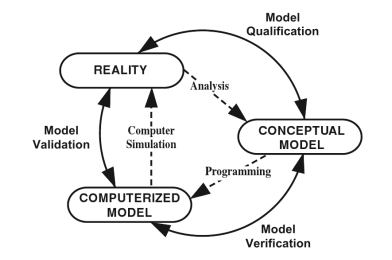
\includegraphics[width=.7\linewidth]{schelinger_schema1979.png}
	  \end{sidecaption}
\end{figure}

\foreignblockquote{english}[\cite{Oberkampf2010}]{The \textbf{conceptual model} comprises all relevant information, modelling assumptions, and mathematical equations that describe the physical process or process of interest. [...] The SCS defined \textbf{qualification} as \enquote{Determination of adequacy of the conceptual model to provide an acceptable level of agreement for the domain of intended application}. The \textbf{computerized model} is an operational computer program that implements a conceptual model using computer programming. Modern terminology typically refers to the computerized model as the computer model or code.}

Ce schéma a la particularité suivante, il \foreignquote{english}{ [...] emphasizes that \textbf{verification} deals with the relationship between the conceptual model and computerized model and that \textbf{validation} deals with the relationship between the computerized model and reality. These relationships are not always recognized in other definitions of V\&V [...]}

Autrement dit, \foreignquote{english}{The OR community clearly recognized, as it still does today, that V\&V are tools for assessing the accuracy of the conceptual and computerized models.} Un avis partagé par \textcite{Kleijnen1995}\Anote{Kleijnen_def}, \textcite{Balci1998}, et \textcite{Sargent2010}\Anote{Sargent_def}.

Seulement, cette forme de relâchement sur la correspondance entre réalité et modèle, et ce positionnement plus relativiste de la validation n'a pas toujours été une évidence; les premières définitions de Naylor par exemple, sont toujours usitées et continuent si on en croit des auteurs comme \textcite{Kleindorfer1998} à semer le trouble dans certaines disciplines.

Mais en excluant ainsi de son analyse la partie subjective et philosophique de la \enquote{Validation}\Anote{VV_philout} pour se concentrer sur la seule partie opérationnelle, ces méthodologies restent pour le modélisateur une coquille vide décevante, qui demande encore à être incarnée thématiquement. Autrement dit, ces méthodes si elles prennent bien en compte la dimension dynamique et incrémentale nécessaire à la construction d'un modèle de simulation qui tendrait vers une réalité en accord avec la question posée, l'organisation des connaissances nécessaires pour guider ce processus reste à la lecture de ces typologies une opération quelque peu énigmatique pour les modélisateurs géographes. On retombe sur une des critiques soulevées précédemment dans la section \ref{sec:critiques_simulation} sur l'absence constatée dans les publications de méthodologie standard pour la validation qui prendrait en compte les problématiques spécifiques d'une discipline.

Une position compréhensible de la part d'auteurs qui oeuvre pour la standardisation de ces termes, alors même que leurs usages restent assez variables selon les disciplines. Une des conséquences visibles tient dans ces incompréhensions et ces débats terminologiques sans fin \autocites{David2009, Augusiak2014} que l'on observe parfois en marge des discussions interdisciplinaires. Cette gamme d'acceptions différentes tient souvent au transfert hasardeux des terminologies entre l'ingénierie des \textit{M\&S}, la philosophie des sciences, et la thématique d'un chercheur en sciences sociales qui se retrouve au croisement des deux discours. Un exercice d'équilibriste périlleux, car comme le fait remarquer \textcite{Kleijnen1995} en citant astucieusement une note de bas de page de \textcite{Barlas1990}, en philosophie il est tout à fait possible de voir la signification des deux termes inversée\Anote{note_barlas}.

\subsubsection{Validation et simulation en philosophie des sciences}
\label{sssec:philo_sciences}

%mais a posteriori, je sais pas, je me dis que tu pourrais peut-être nous guider un peu plus au début par quelques phrases d’intro et des sous-sections, pour qu’on sache ou on va :
%- du cadre général des philosophes des sciences
%- aux comparaisons simu / expérience physique
%- à la critique de tout ça (ou à une autre perspective au moins)  en science sociale

Après avoir donné quelques éléments de débats dans le cadre général des philosophes des sciences, il sera proposé de glisser peu à peu vers la mise en place de critiques de nature différente, car provenant cette fois-ci des praticiens. Une première critique de Peschard (physicienne) \autocite{Peschard2013} sera mobilisé afin de montrer que même en physique ce débat est loin d'être évident. Puis une seconde critique de ce cadre d'analyse sera amené du point de vue des sciences humaines et sociales, et de la géographie.

\paragraph{Mise en place et débats au sein d'un cadre général en philosophie des sciences}

%redite : L'objectif n'est donc pas tant de développer une argumentation critique exposant l'ensemble de ces points de vue, car ce n'est pas l'objet de cette thèse, que de tenter de s'insérer (et non de s'enfermer) dans ces réflexions en spécifiant en quoi celles-ci diffèrent, négligent ou font peu écho à nos pratiques et réflexion historique en sciences sociales.

Il ne s'agit pas de se lancer ici dans un exposé historique des courants et débats s'étant succédés dans cette discipline, mais d'amener de façon illustrative et avec quelques références récentes l'émergence ces vingt dernières années d'une \enquote{épistémologie de la simulation} reprenant (en parasitant parfois le débat comme on l'a cité au-dessus) de son point de vue certains débats évoqués chez les praticiens de la simulation; la question de validation traitée dans le chapitre 1 étant un sujet de longue date chez les praticiens de la simulation, mais aussi chez les premiers acteurs fondateurs de la \textit{V\&V}.

Le premier obstacle avec laquelle les acteurs supportant cette nouvelle épistémologie doivent cohabiter est évidemment la contre-argumentation questionnant cette même nécessité d'opérer une nouvelle sous-division épistémologique. Car existe-t-il réellement des spécificités à la connaissance dérivée de l'étude de l'objet simulation, et si oui quelles sont-elles réellement ? Autrement dit, existe-t-il une différence fondamentale entre les questionnements déjà posés dans le cadre d'une épistémologie des modèles et ceux évoqués dans le cadre d'une épistémologie de la simulation ?

Parmi les auteurs ouvertement favorables à la création d'une nouvelle épistémologie, on citera entre autre les efforts d'Eric Winsberg \autocites{Winsberg2001, Winsberg2009, Winsberg2013} qui pousse dans chacune de ses publications les \enquote{philosophes des sciences} à sortir de la seule étude de la \enquote{théorie de la confirmation} pour aller vers un terrain un peu plus aventureux\Anote{frilosite_philoScience}, celui de l'étude originale\Anote{originalite_epistemologie} de la crédibilité des explications et des hypothèses dans leur dépendance au contexte, ce qui n'est pas sans soulever un certain nombre de critiques\Anote{critique_positionnement}.

Le deuxième point de débat intéressant réside dans le qualificatif souvent donné à la simulation de \enquote{laboratoire virtuel pour l'expérimentation}. Si les philosophes des sciences ne peuvent que s'incliner face au constat d'une telle banalisation du terme, dont nous avons donné nous-mêmes un aperçu de son ancienneté d'usage dans les sciences sociales dans le chapitre 1; il existe quand même chez les philosophes des sciences la volonté de mettre à l'épreuve les fondements et les conséquences pour la connaissance extraite d'une telle analogie. Peut-on comparer la connaissance construite par l'expérimentation réelle et l'expérimentation produite le cadre d'une simulation ?

Mais cette question en appelle d'autres, et pour que ce débat puisse être mené, il faut normalement préciser de quels types de modèles parle-t-on lorsqu'on parle de \enquote{modèles de simulation}, ou de \enquote{simulation de modèle}. On a déjà précisé dans la section \ref{p:autre_def_modele} notre attachement à une définition plus dynamique et moins formelle du modèle \autocites{Haggett1965,Langlois2005} tout en assumant une vision de la simulation algorithmique et/ou à base de règles \autocite{Varenne2013b}. Il faut noter que cette question du rapport entre modèles et simulation est considérée par certains épistémologues comme un objet de recherche à part entière. Sur ce point on renvoie explicitement le lecteur à l'analyse détaillée réalisée par \textcite{Varenne2013b}, et à la typologie très complète qu'il a proposé, car cette question de recherche est souvent traitée de façon assez légère par les philosophes des sciences, y compris chez les partisants d'une épistémologie spécifique à la simulation comme Winsberg.

On rappellera seulement ici quelques éléments d'éclaircissements amenés par Franck Varenne lors d'un entretien par email en Septembre 2014 sur cette question. Des éléments traités en détail dans un article daté de 2013 \autocite{Varenne2013b}, dont les citations ci-dessous sont tirées.

\blockquote[\cite{Varenne2013b}]{Un modèle c'est donc un objet médiateur qui a pour fonction de faciliter une opération cognitive dans le cadre d'un questionnement orienté, opération cognitive qui peut être de cognition pratique (manipulation, savoir­ faire, apprentissage de geste, de techniques de conduites, etc.) ou théoriques (récolte données, formulation d'hypothèses, hypothèses de mécanismes théoriques, etc.)}

Ce qui correspond donc à une fonction générale de la notion de modèle, que l'on peut donc dérouler en fonctions spécifiques regroupées sous des types de médiation facilitante (voir la typologie en 20 fonctions réalisée par \textcite{Varenne2013b}). L'extraction de type de médiation facilitante (\enquote{faciliter une expérience} par exemple) revient à définir également une liste d'opérations cognitives théoriques et/ou pratiques qui se rapporte à ce type de médiation.

Par fonction cognitive, il faut comprendre fonction au sens des fonctions épistémiques, équivalentes à des types de médiation facilitante. Ces dernières pouvant être comprises comme une liste d'opérations cognitives théoriques/pratiques\Anote{mediation_facilitante}.

\blockquote[\cite{Varenne2013b}]{En fait, contrairement aux modèles en général, une simulation est caractérisée non pas tant par l'unité d'une fonction cognitive qu'elle assurerait toujours sous une forme ou sous une autre que par son fonctionnement interne, fonctionnement qui, bien sûr, mais selon seulement secondairement, se trouve avoir aussi des conséquences sur sa ou ses fonctions cognitives.}

Par le terme \enquote{qu'elle assurerait toujours sous une forme ou sous une autre} il faut comprendre aussi \enquote{qu'une simulation est certes une opération mettant en oeuvre toujours des symboles (comme un modèle) mais qui est non toujours prioritairement orientée sujet (à la différence d'un modèle).}

Il peut donc y avoir simulation sans qu'il y ait de fonctions cognitives mobilisées à l'origine. Franck Varenne conçoit en effet la simulation sur ordinateur comme \enquote{une technologie, un procédé technique} automatisant des opérations sur des entités qui \enquote{ doivent être nécessairemenent conçues comme des symboles}. Cette technologie en elle-même ne nécessite pas l'existence de la fonction de modèle, ou de la mobilisation de fonctions cognitives. Ce qui n'empêche pas leur émergence pendant l'exécution, ou a posteriori à la suite de cette exécution.

Nous n'irons pas plus loin dans ce débat, mais il faut toutefois garder à l'esprit qu'il impose l'introduction \autocite{Phan2010, Varenne2013b} d'un nouvel angle d'analyse au débat sur l'expérimentation tel qu'évoqué ci-dessous chez Winsberg. Il pose en effet la question de savoir comment est introduit par les modélisateurs ce rapport à l'empirie \textit{kind of empiricity} censé permettre le dégagement de connaissances de ces quasi-expérimentations que sont les modèles de simulations \autocite{Phan2010} ?

Pour revenir au débat sur \enquote{la simulation comme expérimentation}, afin de ne pas trop se perdre dans les différents points de vue sur le sujet et de  bénéficier d'une vue plus large incluant les réflexions d'épistémologues (plus) praticiens, on pourra se référer au travail opéré par \textcite{Varenne2001} dans son article \textit{What does a computer simulation prove?}, qui propose une lecture du débat au travers d'une typologie soulevant trois grandes thèses : I - La simulation est-elle un outil commes les autres \textit{A simulation is only a tool} ? II - ou bien l'équivalent fusionnel d'une expérimentation classique (\textit{A simulation is an experiment}) ? III - ou se positionne-t-elle comme médiateur entre la théorie et expérimentation ? (\textit{A computer simulation is an intermediate between theory and experiment})?

%L'expérimentation mène sa vie propre et entretient diverses relations avec la spéculation, le calcul, la construction de modèles, l'invention et la technologie. Mais alors que le calculateur, le spéculateur et le constructeur e modèles peuvent être anti-réalistes, l'expérimentateur, lui, doit être réaliste. p18

%On trouve donc un grand nombre de travaux, toutes disciplines confondues (les philosophes des sciences ne sont pas les seuls à se poser ce type de question, comme nous verrons par la suite), qui tentent d'établir par le biais de différentes grilles de lecture l'appartenance de ce \enquote{nouveau?} mode d'expérimentation à une des catégories de cette grille. \textit{Pourquoi ? Au delà du jeu d'esprit, quel est l'enjeu motivant une telle comparaison ?}

On s'appuiera dans la suite de cette argumentation sur la lecture de Winsberg, un philosophe des sciences que l'on estime plutôt partisan de la thèse III dans la classification ci-dessus.

Ce débat de positionnement est d'autant plus actif qu'on assiste depuis ces 20 dernières années à un véritable renouveau des questionnements dans le cadre d'une \enquote{épistémologie de l'expérimentation} jusqu'alors relativement peu considérée par la majorité des philosophes des sciences\Anote{Phan_Varenne_theorie}. \textcites{Phan2008, Phan2010} citent ainsi les contributions importantes d'auteurs comme Fischer (1996), Galison (1987, 1997), Franklin (1986, 1996), Morrisson(1993, 1999), mais également les efforts de Hacking (1983) et Cartwright.

Partant du fait que l'expérimentation joue un grand rôle dans l'établissement d'une crédibilité pour les hypothèses avancées, il s'agit de mesurer à quel point la simulation serait susceptible d'apporter les mêmes garanties dès lors qu'on accepte de la voir comme une sorte d'expérimentation, au sens le plus appliqué du terme lorsqu'il s'agit de mesurer la \enquote{réalité} physique des phénomènes\Anote{experimental_warranting_belief}. Winsberg n'hésite pas à débattre pour ce qui est des différents parallèles que l'on peut tracer avec les réflexions de cette communauté\Anote{winsberg_exper_simu_link}. Il fait ainsi appel directement à Hacking et Galison pour construire sa réflexion, par exemple en arguant \foreignquote{english}{ [...] that some of the techniques that simulationists use to construct their models get credentialed in much the same way that Hacking says that instruments and experimental procedures and methods do; the credentials develop over an extended period of time and become deeply tradition-bound.} \autocites{Winsberg2003, Winsberg2013}\Anote{moto_hacking}.

De cet argumentaire, on retiendra principalement cette propriété d'indépendance retrouvée de l'expérimentation par rapport à la théorie\Anote{def_cartwright}, dont on peut trouver un très bon manifeste dans les écrits de \textcite{Hacking1989} et Cartwright\Anote{def_hacking}, ces derniers se positionnant comme des antiréalistes des théories, tout en étant des réalistes des entités théoriques. Un point de vue très bien résumé à la fois dans \textcite{Hacking1989} et dans l'ouvrage \textit{Théorie, Réalité, Modèle} de \textcite[226-231]{Varenne2012}. Un consensus semble se dégager chez plusieurs philosophes \autocites{Morgan2009, Varenne2001, Varenne2013b} dans la lignée de cette propriété, le modèle étant perçu comme un \enquote{médiateur autonome} articulant théorie, pratiques et données dans un contexte spécifique d'une question et d'un cadre technico-social \autocite[2]{Phan2010}\Anote{varenne_autonome}.

Dans un but pédagogique, il me semble intéressant de revenir sur l'établissement d'un tel consensus, en évoquant plus en détail toute la complexité développée dans ce débat sur le positionnement de la simulation vis-à-vis de l'expérimentation. On peut s'appuyer sur le discours de Winsberg qui propose une lecture en deux thèses opposées : \foreignquote{english}{Identity Thesis} qui consiste à dire que la simulation est littéralement une expérimentation, et \foreignquote{english}{Epistemology Identity Thesis} qui consiste à penser qu'il existe une dépendance entre les garanties de crédibilité qui pourront être accordées par les résultats de la simulation et la capacité des simulations à être plus ou moins définies en tant qu'expérience. Si la première thèse semble assez bien correspondre au point I de la classification de Varenne, la deuxième semble être une sous-variation du point I.

La plupart des auteurs cités par la suite dans ce débat sont des philosophes des sciences spécialisés en économie (Guala , Morgan, Maki, Simon ) qui rejettent comme Winsberg (plus spécialisé en physique) assez naturellement ces deux thèses \autocite{Winsberg2009}, mais avec des arguments assez différents, qu'il convient d'évoquer pour bien comprendre la complexité de ce débat, assez théorique.

Parmi les différents point de vue existants, on citera par exemple le sous-débat de l'\foreignquote{english}{isolative analogy} relaté ici au travers des publications de \textcite{Phan2008, Phan2010} appelant les points de vue de Morgan et Guala contre Maki (2005). Ce dernier voit dans la similitude entre isolement théorique du modèle comme expérience de pensée et isolement expérimental\Anote{maki_phan} la possibilité de rejoindre une des deux thèses évoquées par Winsberg, établissant d'une façon ou d'une autre que \textit{les modèles sont des expériences, et les expériences des modèles}. Mais ce type d'argument, et on le suppose tous ceux qui se rapportent à l'évocation d'analogies pour justifier d'une équivalence de puissance épistémique se heurteraient, comme on va le voir, à une différence fondamentale.

\textcite{Phan2010} et \textcite{Winsberg2013} citent le point de vue de Guala (2002, 2008), partagé par Morgan (2002, 2005) et se référent aux travaux de Simon (1969). Ceux-ci s'appuient sur une différence de relation qui existe entre système à étudier et système cible dans chacun des deux cas. En effet, dans le cas des expériences, la comparaison s'appuie avant tout sur une similarité matérielle, alors que dans le cas de la simulation la comparaison est limitée à une comparaison formelle entre les objets.\Anote{guala_phan_winsberg}

Morgan(2002, 2005) accepte le point de vue Guala et Simon, mais s'en sert pour réduire indirectement le pouvoir épistémique de la simulation. Un argument bien résumé par \textcite{Phan2008} \enquote{Pour Morgan (2005) les modèles et expériences partagent des fonctions de médiateurs et peuvent fonctionner \textit{sur un mode expérimental}, mais les expériences \textit{réelles} offrent un \textit{pouvoir épistémique} d'investigation de la réalité empirique plus fort.}  Ce qui fait dire à Winsberg que Morgan serait indirectement plutôt partisan de sa deuxième thèse\Anote{Winsberg_critique_morvan}. Autrement dit, comme la simulation et l'expérimentation seraint effectivement différentes (rejette l'\textit{identity thesis}) , les capacités explicatives de la simulation en ressortiraient amoindries (accepte l'\textit{Epistemology Identity Thesis}).

Pour \textcite{Winsberg2009} le flou des arguments avancés par Guala  (\textit{material similarity}, \textit{mere formal similarity}) ne sont pas convaincants, et ne permettent pas en l'état d'exclure complétement et définitivement la première thèse\Anote{winsberg_mereformal}. Celui-ci se range malgré tout du côté de Guala sur le fond, et préfère là aussi rejetter cette thèse (rejette l'\textit{identity thesis}), mais à la faveur de sa propre argumentation; ce qui lui permet au passage de rejetter l'argument de Morgan qui voit dans les arguments de Guala la possibilité de pointer l'infériorité épistémique de la simulation, et donc d'adopter l'\textit{Epistemology Identity Thesis}. Winsberg refute donc les deux thèses. Il argue que les simulations et l'expérience diffèrent principalement par la nature du \textit{background knownledge} (rejette l'\textit{identity thesis}) , c'est-à-dire les protocoles et les connaissances mobilisés. Pour lui, c'est sur cette seule base qu'on pourrait juger des capacités epistémiques de la simulation (rejette l' \textit{Epistemology Identity Thesis}). Winsberg conclut en ajoutant que l'expérimentation, contrairement à ce que l'on pourrait penser, n'est pas forcément et immédiatement plus crédible si on ne lui ajoute pas un bagage de connaissances : \textit{Experiments are not automatically more reliable than simulations, despite their differences. [...] It would seem that there are identifiable differences between ordinary experiments and simulations, but there is nothing about these differences that makes one or the other intrinsically more epistemically powerful.}  \autocites{Winsberg2009, Winsberg2013}

\textcite{Varenne2001} avance alors un autre argument intéressant, et pointe comme le fait aussi Winsberg, la possibilité de voir dans les simulations des résultats parfois plus convaincants que de véritables expérimentations : \foreigntextquote{english}[\cite{Varenne2001}]{Indeed, when you read (Von Neumann 1951), you see that analog models are inferior to digital models because of the accuracy control limitations in the first ones. Following this argument, if you consider a prototype, or a real experiment in natural sciences, is it anything else than an analog model of itself? The test on the prototype is a real experiment. But is it something different and better than the handling of an analog model? So the possibilities to make sophisticated and accurate measures on this model - i.e. to make sophisticated real experiment - rapidly are decreasing, while your knowledge is increasing. These considerations are troublesome because it sounds as if nature was not a good model of itself and had to be replaced and simulated to be properly questioned and tested! It looks as if it was not possible any more to end a paper on simulation by reassuringly using the traditional word: \enquote{Simulation will never replace real experiments}. }

Ces derniers paragraphes montrent que le débat est encore loin d'être fixé, et il semblerait là encore que ce soit la définition du contexte d'application qui détermine le mieux la capacité explicative de la simulation, car comme le dit Winsberg \enquote{l'impossibilité d'expérimenter} existe dans bien des disciplines, comme les sciences sociales, mais également la biologie ou la physique, où les tentatives de reconstitution simulées d'univers ou d'étoiles dans des super calculateurs de plus en plus puissants montrent qu'il existe un intérêt explicatif à cette pratique. On pensera notamment aux projets d'expérimentation récents extrêmement complexes et coûteux en physique (laser megajoule de Bordeaux, projet ITER pour la fusion).

Des modélisateurs et épistémologues en sciences sociales beaucoup plus proches de nos pratiques comme Phan et Varenne trouvent un argument convaincant dans ce dernier point, car \foreignquote{english}{Aujourd'hui, comme le souligne Winsberg, la crédibilité des modèles de simulation repose largement sur la \textit{confiance} que nous pouvons avoir dans les compétences des modélisateurs, informaticiens, expérimentateurs et observateurs, ainsi que dans les composants ou plateformes qui supportent les expériences de simulation.} \autocite{Phan2008}

\paragraph{Controverse, la critique d'Isabelle Peschard}

La façon dont Winsberg construit son argumentaire n'est pas forcément acceptée en tant que telle par les praticiens, ce qui nous permet d'introduire ici un sous-débat faisant suite au débat précédent. On revient ainsi sur la critique de l'\textit{identity thesis} comme évoquée par Gilbert et Troitzsch (1999). De façon générale, on a vu que Winsberg pense\Anote{gilbert_critique}, en accord avec Guala (2002) \autocite{Winsberg2009} mais également Morgan\Anote{guala_morgan_reality_experiments} et Parker \autocite{Winsberg2013}, que cette critique avancée par Gilbert et Troitzsch est trop faible pour rejeter l'\textit{identity thesis}. C'est ce qui pousse chacun d'entre eux à formuler des arguments plus convaincants, soit en défense de l'\textit{identity thesis} (Parker), soit dans le rejet de l'\textit{identity thesis} (Morgan, Guala, Winsberg). Ces arguments contre l'\textit{identity thesis}, puis contre l' \textit{Epistemology Identity Thesis} (Winsberg) ont été évoqués précédemment, on ne reviendra donc pas dessus ici, pour se concentrer sur le débat de Winsberg avec la praticienne et physicienne Isabelle Peschard.

Si les arguments de Winsberg semblent, selon Isabelle Peschard \autocites{Peschard2010b, Peschard2013}, assez convaincants, celle-ci tente dans une analyse critique de montrer le biais qui existe dans les prémisses de son argumentaire, et apporte dans son article des objections tout à fait crédibles issues de son domaine d'expertise. Pour ne citer qu'un de ses arguments, s'il existe bien un intermédiaire de mesure issue d'un modèle, comme l'indique Winsberg, il existe également un sous système en prise directe avec la réalité physique de ce monde.

\blockquote[\cite{Peschard2013}]{Il est généralement admis que, dans le cas de la simulation, l'objet manipulé et le système cible sont clairement distincts. La question est de savoir si la même distinction peut être faite dans le cas de l'expérience. [...] Tous deux [Guala et Winsberg] considèrent donc que le système manipulé et le système cible sont des systèmes différents dans le cas de la simulation et de l'expérience. La différence entre simulation et expérience se trouve, selon eux, ailleurs. [...] Selon Winsberg, la différence, qui est importante, est épistémologique : elle est au niveau de la justification de l'inférence qui mène des résultats portant sur le système manipulé à l'information sur le système cible.}

\blockquote[\cite{Peschard2013}]{Une prémisse cruciale de la démonstration, toutefois, est qu’aussi bien dans le cas de l’expérience que de la simulation, le système manipulé est un système différent du système cible, un système qui représente le système cible, dans le sens de \enquote{ tenir lieu de }. Mais il y a, comme nous allons voir, des raisons de douter de cette prémisse. Premièrement, il ne semble pas nécessaire, contrairement au cas de la simulation, que dans le cas de l’expérience le système manipulé soit différent du système cible. Deuxièmement, quand ces deux systèmes sont différents, la relation entre eux est très différente de ce qu’elle est dans le cas de la simulation.}

En conclusion, elle estime que s'il y a bien une certaine forme de similarité entre cibles épistémiques de la simulation et de l'expérience, ces activités ne peuvent pas être considérées comme épistémiquement équivalentes, ce qui n'empêche en rien selon elle la coopération fructeuse des deux approches, simulation et expérimentation.

\textcite{Winsberg2013} résume le point de vue de \autocite{Peschard2010} ainsi, \textit{Thus, simulation is distinct from experiment, according to her, in that its epistemic target (as opposed to merely its epistemic motivation) is distinct from the object being manipulated.} Autrement dit, l'objet manipulé dans une expérience est bien celui du monde physique, alors que dans le cas de la simulation c'est l'ordinateur. Or, autant on peut apprendre d'un objet manipulé dans le monde physique, autant il n'est pas ici dans notre intérêt d'apprendre sur l'ordinateur en tant qu'objet. Dans ce cas là on pointe une différence, mais on peut également appeler selon \textcite{Winsberg2013} et Morrisson (2009) l'argument inverse, en pointant au contraire une similarité. L'objet expérimenté peut en effet être choisi par l'expérimentateur en tenant compte justement de sa capacité de \textit{surrogate} rapport à la question que l'on se pose effectivement, un point commun entre la construction de simulation et d'expérimentation.

On n'a fait ici qu'effleurer et simplifier des débats théoriques beaucoup plus complexes. Cette dernière sous section a permis de faire émerger les différences qui pouvaient exister entre un discours sur la modélisation finalement assez théorique, et un autre discours, plus \foreignquote{english}{bottom up}, provenant des pratiques des modélisateurs. Dans la section suivante, on propose de continuer ce glissement en confrontant ces discours théoriques à une pratique de la modélisation en géographie.

\paragraph{Des débats très éloignés des pratiques de modélisation en géographie}

Winsberg est plus un spécialiste des sciences physiques. Or, en acceptant d'intégrer l'importance du contexte dans la justification de cette puissance épistémique de la simulation dans son argumentaire, celui-ci est également contraint de reconnaître de façon prudente les conséquences que peut avoir une telle inclusion dans la solidité de sa synthèse.

\foreignblockquote{english}{Parker (forthcoming) has made the point that the usefulness of these conditions is somewhat compromised by the fact that it is overly focused on simulation in the physical sciences, and other disciplines where simulation is theory-driven and equation-based. This seems correct. In the social and behavioral sciences, and other disciplines where agent-based simulation (see 2.2) are more the norm, and where models are built in the absence of established and quantitative theories, EOCS probably ought to be characterized in other terms.

For instance, some social scientists who use agent-based simulation pursue a methodology in which social phenomena (for example an observed pattern like segregation) are explained, or accounted for, by generating similar looking phenomena in their simulations (Epstein and Axtell 1996; Epstein 1999). But this raises its own sorts of  epistemological questions. What exactly has been accomplished, what kind of knowledge has been acquired, when an observed social phenomenon is more or less reproduced by an agent-based simulation? Does this count as an explanation of the phenomenon? A possible explanation?
(see e.g., Grüne-Yanoff 2007).

It is also fair to say, as Parker does (forthcoming), that the conditions outlined above pay insufficient attention to the various and differing purposes for which simulations are used (as discussed in 2.4). [...] Indeed, it is also fair to say that much more work could be done in classifying the kinds of purposes to which computer simulations are put and the constraints those purposes place on the structure of their epistemology.}

Des philosophes des sciences ont donc saisi cette opportunité de critiquer l'approche de Winsberg pour soulever dans des tentatives de typologies parfois intéressantes \autocite{Eckhart2010} les points de divergence que soulève l'utilisation d'une philosophie des sciences naturelles inadaptée à la simulation en sciences sociales. Malheureusement, au cours de ces mêmes lectures, on constate que cette critique se retourne vers les modélisateurs et praticiens des sciences sociales, et mène cette fois-ci dans une analyse incomplète du contexte historique au mieux à des interprétations erronées (voir le débat animé entre \autocite{Yanoff2008}  \autocites{Elsenbroich2012, Chattoe2011}), et au pire à des approximations et conseils de mise en oeuvre totalement déplacés \autocite{Eckhart2010} vis-à-vis de disciplines qui disposent comme on l'a vu d'une véritable histoire autour de l'usage des méthodes computationelles.

Car bien que la recherche des points communs et des différences entre réalité de l'expérimentation physique et virtuelle apparaisse comme un débat intéressant, il faut bien avouer que celui-ci ne peut que difficilement s'adapter à la quasi absence d'expérimentation au sens classique dans les sciences sociales. Ainsi, même si la simulation partage certaines des propriétés de l'expérimentation classique, il y a quand même quelque chose de paradoxal à vouloir absolument analyser le rapport de la simulation à l'expérimentation alors même que c'est cette absence qui justement motive son utilisation dans notre discipline, hormis peut-être pour mettre plus en avant cette incapacité à formuler un unique cadre fédérateur par un tel débat. Comme le dit très justement \textcite{Phan2008} {[...] les sciences économiques et sociales sont plus volontiers concernées par l’opposition entre \enquote{le modèle et l’enquête}  (Gérard-Varet et Passeron, 1995) que par celle entre \enquote{l’expérience et le modèle} (Legay, 1997)}.

La notion de modèle vue comme médiateur autonome entre théorie et expérimentation doit elle aussi être repensée pour les sciences humaines et la géographie; car les théories si elles peuvent exceptionnellement servir à dériver des modèles, elles ne peuvent qu'être difficilement rapportées à leur équivalent en sciences physiques \autocite{Pumain1997}.

D'un côté, les sciences physiques semblent encore viser à l'établissement d'un cadre fédérateur alors qu'il semble que les théories et les modèles en sciences sociales - hormis peut-être le cas particulier de l'économie - soient au contraire pourvoyeurs de richesse dans leur capacité à apporter un nouvel éclairage sur un phénomène observé.

A cela, il faut ajouter que le modèle en géographie opère dans un cadre épistémique particulier qui n'est pas forcément celui de toutes les sciences humaines. Ainsi, bien que les notions et le rapport entre les notions d'observation du \textit{singulier} et du \textit{général} soient théoriquement à la portée de toutes disciplines \autocite{Dastes1992}, il semblerait que la géographie trouve un intérêt particulier pour la constitution de sa démarche explicative à articuler des éléments de connaissance pris dans les grandes familles explicatives historiques, écologiques, et spatiales; justifiant ainsi de niveaux d'explication plus ou moins en interaction mobilisant chacun des déterminants de nature différente. Avec la possibilité d'intégrer à tout moment dans l'explication les résidus qui tiennent d'un dialogue entre mécanismes généraux et singularité historique, écologique ou spatiale. Car quelque soit le registre explicatif choisi, il reste dans les deux cas \textit{ [...] une part d'explication relevant de ce que l'on peut qualifier de singularités locales, non prédictibles à partir de mécanismes généraux, mais nécessitant d'appréhender l'histoire spécifique du lieu}. La conséquence étant une diversité de modèles support de l'\textit{explanan} (l’explication que l’on propose du phénomène auquel on s’intéresse) dont l'évolution sur la forme et le fond n'a eu de cesse d'éclairer l'\textit{explanandum} sous un jour différent \autocite{Dastes1992, Sanders2000, Sanders2013}.

En 1986, lors d'un débat sur les apports de l'\textit{Artificial Intelligence} (AI) en géographie, avec notamment les apports de la branche discrète de la simulation (Automate Cellulaire par exemple), Couclelis montre que les considérations philosophiques abordées jusqu'ici sont en réalité très vite abordées par les géographes.

\foreignblockquote{english}[\cite{Couclelis1986}]{A further insight to emerge from discrete model theory, which has some interesting philosophical implications, deserves a few comments. The widespread belief that proposing a model corresponds to the assertion that the real phenomena must have some similar structure is contradicted by the sharp distinction between structure and behavior drawn in discrete model theory. Although structure governs behavior, the converse is not true, so that obtaining a model that reproduces some behavior well does not entitle one to make any inferences about the \enquote{real} structure of the phenomenon represented. In fact, it is doubtful whether we may talk about the structure of real phenomena in other than a metaphorical sense. A real system may be no more than the universe of potentially acquirable data.}

L'éclairage sur la méthodologie sous-jacente à la construction des modèles, pourtant un élément au coeur du raisonnement dans la discipline géographique depuis la révolution quantitative, a encore moins de chance d'être évoqué dans ces publications philosophiques, au détriment d'une réflexion statique plus axée sur la nature de l'objet simulation, et de sa relation au monde.

Or, l'évolution des réflexions touchant l'activité de modélisation se construit il me semble à une échelle de réflexion tout à fait différente, celle historique et contextualisée des pratiques guidées par la résolution de questions spécifiques à l'analyse spatiale. Une activité dont la mise en oeuvre s'appuie sur une chaîne de traitements flexibles susceptibles d'utiliser à bon escient et de façon cumulative des outils dont on connait aussi leurs capacités à renouveler les questionnements : les statistiques, les modèles, les modèles de simulation.

\Anotecontent{Ce qui n'est pas sans nous rappeller les difficultés évoquées dans le chapitre 1 sur l'inadéquation et le danger que représentent les modes de transmissions actuels.}

\Anotecontent{remarque_Varenne_2001}{\foreignquote{english}{The second thesis of this article is that none of the three categories of arguments could be applied to contemporary sciences in general, whatever their objects, their methods and the moment of their history we consider. None of these three categories could be considered as the only true one. We cannot have a general point of view on the value of computer simulations, because of the different implications and meanings of mathematics in the different fields of science, and because of the various philosophies of nature at stake. This fact remains true for a given field throughout its own history, because the role of mathematics and the definition of the studied object evolve: You cannot find a unique and stable value that would be given to its simulation uses once for all. Again and hopefully, this thesis illustrates the fact that it does not belong to the historian to decide on the value of computer simulation in a given field but to the scientists themselves. These preliminary reflections prove the importance to investigate the intellectual history of contemporary sciences and not only their sociological construction nor their philosophical general insights.}\autocite{Varenne2001}}

Ces rapides remarques nous éclairent sur la latence qui existe entre la réflexion récente d'épistémologues comme Winsberg, Grüne-Yanoff et la réalité théorique et pratique en géographie. \textcite{Varenne2001} avait déjà bien cerné dans la synthèse faite en 2001 qu'il n'y avait pas dans sa classification une position meilleure ou plus convaincante qu'une autre, la réponse se trouvant comme pour la notion de modèle avant tout dans l'étude du contexte, et donc de l'histoire des disciplines face à cet objet simulation\Anote{remarque_Varenne_2001}. Cela ne veut pas dire que les débats évoqués précédemment en sont automatiquement invalidés, seulement qu'il faut être probablement plus regardant vis-à-vis des remarques générales et des conclusions beaucoup trop hâtives qui peuvent parfois en découler.

Les travaux croisés de certains praticiens, d'épistémologues ou historiens des sciences propres à la géographie ou s'en approchant permettent d'une part d'apposer un premier filtre sur ces réflexions génériques pour s'y référer prudemment, et d'autre part d'innover en questionnant nos démarches dans ce qu'elles ont d'originale, cette fois-ci appuyées sur une lecture des pratiques certes pas toujours parfaites mais pouvant au moins être qualifiées de \textit{bottom-up}.

%\hl{Un travail conséquent à la croisée de différentes approches, les travaux d'historiens et épistémologues des sciences somme Orain, Besse, Cuyala, et la lecture plus spécifique de l'évolution des méthodes numériques puis computationelles et de leur apports d'un point de vue pratique et théorique dont on trouve source à la fois dans les nombreux travaux des praticiens, mais également dans des travaux de plus long cours comme celui qu'est en train de réaliser Varenne dans son HDR.  == REDITE}

%\hl{ont su voir rapidement l'intérét de développer plus en avant les spécificités attachés à la simulation en science sociale, déjà riche de réflexion sur les apports successifs et cumulatifs de techniques de simulations \autocites{Banos2013, Varenne2008}, en s'intégrant au débat d'une communauté inter-disciplinaire structuré autour de la modélisation agent, qui émerge dans les sciences sociales au début des années 1990. Ce débat par contre ne fait semble-t-il que commencer dans le courant plus \textit{mainstream} des philosophe des sciences.}

%tel que celle des géographes pratiquant la simulation depuis les années 1950, tels que celle qui a émergé autour de la modélisation agent dans les années 1990.

%Ainsi comme on a pu le voir dans le chapitre 1, le terme laboratoire virtuel pour l'expérimentation apparait très tot dans les sciences sociales, et des auteurs ont pour l'époque déjà donnés de très bonne raisons pour l'emploi de ce terme; les aspects dynamiques de la simulation en faisait partie.

\subsubsection{La Validation vue par une communauté de modélisateurs}
\label{sssec:validation_modelisateurs}

Depuis le début des années 1990 et la diffusion progressive du méta-formalisme Agent \autocite{Treuil2008} dans les sciences humaines et sociales, les modélisateurs géographes peuvent, en plus des pratiques internes à la géographie, se tourner vers les discussions opérées dans une communauté d'acteurs modélisateurs internationaux et interdisciplinaires. On trouvera à ce sujet une tentative d'exploration des fondements historiques de ce mouvement dans l'annexe \ref{chap:double_foyer_sma}. Sorti des ouvrages fondateurs, et des ouvrages plus disciplinaires, c'est principalement autour du \textit{Journal of Artificial Societies and Social Simulation} (JASSS) fondé en 1998 que gravitent la plupart des discutants pertinents sur la problématique de la Validation.

\paragraph{Persistance historique et limites des guides méthodologiques}

Cette étape de Validation, l'écueil sûrement le plus important, est pourtant souvent évoquée comme une étape cruciale dans bons nombres de guides méthodologiques pour \enquote{la bonne construction des modèles}, qu'ils soient anciens \autocites[195]{Beshers1965}{Guetzkow1972, Dutton1971,Naylor1966, Naylor1967}, ou plus récents \autocite{Amblard2006, Gilbert2008}.

Cette constance, on la retrouve d'abord assez logiquement chez les pionniers utilisateurs de la simulation algorithmique (à la différence de la résolution mathématique), comme \textcite{Doran1975, Doran1986} qui introduit les DAI chez les sociologues avec Gilbert dès 1985 \autocite{Gilbert1985}, ou chez les archéologues en 1980 au colloque de Southampton \autocites{Doran1982, Renfrew1982} (voir annexe déjà citée ci-dessus). Ainsi à la lecture des écrits de \textcite[300-301]{Doran1975} sur la simulation dans \textit{Mathematical Models and Computer Simulations}, on s'aperçoit d'une part qu'il est déjà très au fait de la littérature inter-disciplinaire existante en simulation \autocite{Guetzkow1972} (voir section \ref{ssec:engouement_sciencesociale}), et d'autre part le fait qu'il propose un protocole de construction de modèles assez similaire à ce que l'on trouve encore aujourd'hui.

\foreignblockquote{english}[\cite{Guetzkow1972}]{Any serious simulation study involves major effort at a number of stages : advanced planning; collection and organisation of suitable data; detailed specification of simulation; writing and initial \enquote{debugging} of the computer program; preliminary testing and validation of the program; it's use in the sequence of experiments designed to achieved specified objectives; and finally the study and interpretation of the results obtained. It is easy to underestimate the magnitude of the total effort required. It is all the more important to have a clear idea of what the simulation study is intended to achieve; either a broad investigation of the behaviour of simuland\interfootnotelinepenalty=10000\Anote{simuland} or, more likely, a determined attempt to examine the behaviour of certain variables of interest (cost? death rate? output? public approval?) and to discover to what extent they can be controlled.}

\interfootnotelinepenalty=5000

L'accent est déjà mis sur l'exploration des modèles, et \textcite[301]{Doran1975} soulèvent d'ailleurs tout de suite après quelques unes des difficultés pouvant venir grever cette tâche. Car comment valider correctement une simulation compte tenu de tous ces problèmes posés par l'expérimentation ?

\foreignblockquote{english}[{\cite[301]{Doran1975}}]{In any simulation, \textbf{validation} is a matter of great importance. How can it be ensured that the model is indeed a reliable guide to reality ? [...] Once simulation has been validated it can be put to useful work. At this point a major problem appears. [...] any stochastic simulation must be run many times, and effectively one is sampling the behaviour of the variable of interest. This makes for much book keeping and for many complications.[...] Simulations poses two unexpected experimental problems. First, the number of variables and parameters in the simulation is liable to be very large, [...] Second, it may prove disconcertingly difficult to comprehend what is going on within the simulation, just as it is often difficult to comprehend a complex part of the real outside world. [...] These problems are of more than purely technical interest. They arise from the use of tool of sufficient complexity that it's details can extend human comprehension to the limit.}

En 2000, même si les termes se sont raffinés, et que de nouveaux problèmes semblent avoir fait leur apparition dans l'usage de ce nouvel outil des DAI (par exemple avec la prise en compte des aspects cognitifs, la possibilité de représenter et de coupler des objets et des formalismes opérant à des niveaux d'abstraction et de spatialisation hétérogènes, etc.), le lecteur n'est pas non plus complétement dépaysé par la description que fait \textcite{Doran2000} des \foreignquote{english}{Hard problems in the use of agent-based modelling} : \foreignquote{english}{Skills and Time requierement ?, Which type of Model?, What level of Abstraction ?, Searching a massive parameter space ? The problem of validation ?}

On est donc étonné de voir \textcites[93-94]{Crooks2012}{Crooks2008} annoncer la spécificité d'un tel défi dans la modélisation multi-agents, alors même que ce problème était déjà identifié de façon plus générique comme lié à la simulation il y a 50 ans \autocites{Naylor1967, Hermann1967}.

\foreignblockquote{english}[{\cite[93-94]{Crooks2012}}]{The seven challenges that we see as important to the development of agent-based models involve the following: the purpose for which the model is built, the extent to which the model is rooted in independent theory, the extent to which the model can be replicated, the way the model might be verified, calibrated and validated, the way model dynamics are represented in terms of agent interactions, the extent to which the model is operational, and the way the model can be communicated and shared with others. [...] While these challenges are reflected within all modelling endeavours and experienced model builders consider them as quite basic, this paper seeks to comprehensively synthesise and reflect on these issues, making them specific to agent-based modellers, and thus alerting them to the pitfalls of past generations of model.}

Sur ce point de la validation et la vérification, Crooks cite pourtant une définition floue et très générique de North et Macal datée de 2007 :

\foreignblockquote{english}[\cite{Crooks2012}]{ Verification is the process of making sure that an implemented model matches its design. Validation is the process of making sure that an implemented model matches the real-world.}. Un peu plus loin il ajoute une autre citation, à propos de la Validation en elle-même, \foreignquote{english}{Validation relates to the extent to which the model adequately represents the system being modelled (Casti, 1997) and in this sense, it involves the goodness of fit of the model to data. However, the validity of a model should not be thought of as binary event (i.e. a model cannot simply be classified as valid or invalid); a model can have a certain degree of validity which of course is encapsulated by various measures of fit (Law \& Kelton, 1991).}

On a vu pourtant qu'un modèle de simulation suivait un ensemble de fonctions épistémiques potentiellement cumulables \autocite{Varenne2013b}, impliquant lors de la construction des modèles des objectifs de validation très différents. Quant à la notion de \enquote{degré de validité}, on verra que celle-ci n'a pas vraiment de sens pour un modèle en sciences humaines et sociales. Cela supposerait notamment l'existence d'un seuil déterminant pour chaque modèle un niveau d'empirie a priori suffisant pour valider celui-ci. Or, une telle limite n'existe pas, et n'a pas de sens dans la reconstruction d'un monde virtuel dirigé par un but explicatif ayant peu de d'affinité avec une recherche de réalisme. Ces points seront discutés et réfutés plus en détail dans la section \ref{ssec:evaluation_construction}.

Si l'on prend par exemple deux des premières étapes du cycle itératif plus global présenté par \textcite{Sargent2010}.

\foreignblockquote{english}[\cite{Sargent2010}]{Conceptual model validation is defined as determining that the theories and assumptions underlying the conceptual model are correct and that the model representation of the problem entity is \enquote{reasonable}  for the intended purpose of the model. Computerized model verification is defined as assuring that the computer programming and implementation of the conceptual model is correct. [...] An iterative process is used to develop a valid simulation model (Sargent 1984a). A conceptual model is developed followed by conceptual model validation. This process is repeated until the conceptual model is satisfactory.} Un peu plus loin, il revient en détail sur ce concept : \foreignquote{english}{Conceptual model validity is determining that (1) the theories and assumptions underlying the conceptual model are correct and (2) the model’s representation of the problem entity and the model’s structure, logic, and mathematical and causal relationships are \enquote{reasonable} for the intended purpose of the model. The theories and assumptions underlying the model should be tested using mathematical analysis and statistical methods on problem entity data. [...] }

De nombreuses questions restent en suspend dans la transposition d'un tel cycle aux SHS. Que veut dire une représentation du système qui serait \enquote{raisonnable} dans un cadre explicatif? Comme puis-je extraire d'un système complexe un réseau d'hypothèses causales \textit{a priori} correctes et validables sur des phénomènes dont la principale qualité est justement d'être insaisissable? Comment validerait-on un modèle conceptuel au préalable d'une implémentation et de premières expérimentations, alors même qu'on mobilise la simulation pour étudier la dynamique d'hypothèses formulées de façon statique? Et surtout, comment peut-on savoir jusqu'où faut-il aller dans les itérations, et la complexité de ce modèle conceptuel en étant ainsi coupé de l'expérimentation? Que faut-il ensuite penser de la vérification lorsque deux implémentations d'une même hypothèse semble correcte, n'y aurait-il pas aussi des implications se rapportant à la validation dans la vérification? Faut-il les tester d'abord ou renvoyer le modèle conceptuel à la validation? Que se passe-t-il lorsque l'implémentation soulève de nouvelles hypothèses ou impose l'ajout d'artefacts techniques biaisant les pures hypothèses exprimées dans le modèle conceptuel? Comment le retour sur le modèle conceptuel est envisagé après expérimentation?

Toutes ces questions qui relèvent d'une activité de modélisation support d'un raisonnement scientifique ne sont que très vaguemment abordées dans ces définitions. Un modélisateur avisé verra sûrement nombres de ces problèmes apparaitrent entre les lignes ou derrière ces mots, ce que dit Sargent étant suffisamment générique pour s'adapter à de nombreux cas, là n'est pas finalement le plus grand problème. Que peut espérer un modélisateur débutant en géographie d'une telle lecture ? Il y a au final un très grand nombre d'informations manquantes liées aux outils, au contexte, à une démarche de modélisation en géographie ou au fait que le modèle de simulation n'est qu'un modèle parmi d'autres, comme on en discute par la suite.

On peut donc se demander, dans le cadre de ces deux publications \autocite{Crooks2008,Crooks2012}, importantes et relativement récentes sur la simulation multi-agents en géographie, quel est l'intérét des auteurs d'apporter au lecteur une telle définition aussi générique, et qui supporte exactement le même type de critiques que celles déjà formulées pour la \textit{V\&V}. En effet, Law \& Kelton étant avant tout reconnus comme des spécialistes de ces questions dans le domaine de la simulation industrielle, et la référence de North \& Macal pointe sur un ouvrage intitulé \textit{Managing Business Complexity: Discovering Strategic Solutions with Agent-Based Modeling and Simulation}.

Un parti pris d'autant plus étrange que les auteurs de ces publications (Crooks, Batty, etc.) sont tout à fait conscients des limites d'une telle définition, qu'ils viennent de façon implicite \textbf{contredire} plusieurs fois dans le reste des points abordés : \textit{The purpose of model}, \textit{theory and model}, \textit{replication and experiment}, \textit{agent representation}, \textit{aggregation and dynamics}, \textit{sharing and dissemination of the model}, \textit{operational modelling}.

Ainsi, contrairement à ce que laisse supposer la citation du point de vue spécifique à la validation, la nécessité d'une validation de la structure interne des modèles est ainsi avancée explicitement dans la partie \textit{theory and model}, \foreignquote{english}{Our concern here however is that the theoretical implications of many agent-based models remain implicit and hidden, often covered by a thick veil of ad hoc assumptions about structure and process as well as a veneer of software interfacing. [...] In short, the scientific standards of the past are often buried in ad hoc model development.}

Cela n'a rien de nouveau, ainsi Doran postulait déjà de façon très vague en 1975, l'importance d'un contrôle de la cohérence interne des modèles pour la validation.

\foreignblockquote{english}{Where data have been collected on the simuland it will be natural to check the simulation against them. It may well be reasonable to use the simulation to generated limited predictions to be tested against the simuland. Factors that will be certainly permit a simulation to be taken more seriously are internal coherence and common-sense plausability.}

En 1994, le discours sur la validation accompagnant l'expérience sur le modèle de simulation de société ancienne EOS paru dans l'ouvrage \textit{Simulating societies: The computer simulation of social phenomena} est cette fois-ci tout à fait limpide :

\foreignblockquote{english}[{\cite[10-12]{Doran1994}}]{The plausibility, by whatever arguments, of the assumptions built into a model strongly influences the degree of confidence that may be placed on the relevance of its behaviour to that of the target system. Also crucial is the degree of experimental validation of the model and the extent to which its behaviour has been fully explored and understood. Little can be learned from an inadequate sample of the model's behaviour. If a model embodies implausible assumptions and cannot be validated, then nothing can be learned from it about the target - though much may be learned about the properties of the model itself and that may be useful. The last difficulty we shall mention here concerns the interpretation of behaviour obtained from a model even when the model has been experimentally validated and its individual assumptions justified. Just because the model is only a model, it always possible to dispute any parallel claimed between its behaviour and that of the target.}

Que faut-il en conclure ? De façon plus générale, et plutôt que de faire appel aux auteurs phares d'un mouvement \textit{V\&V} qui se répètent depuis 25 ans sur cette question \autocite{Sargent1983, Sargent2010}, les géographes ne mériteraient-ils pas l'établissement d'un défi de la \textit{Verification, Calibration and Validation} prenant racine dans l'histoire de la modélisation en SHS, et en géographie quantitative ? C'est-à-dire dans ce qu'elle a appris et construit autour de ses premières confrontations avec la modélisation, puis la simulation, et cela afin de mieux démarquer nos définitions, nos pratiques de validation face aux cadres standardisés assumés destinés à des pratiques essentiellement industrielles ?

Heureusement, Crooks ne s'arrête pas à cette simple citation pour la validation et pointe également les réflexions plus détaillées de géographes comme \textcites{Batty2001, Batty2005b} sur ces questions. Notre analyse dans la section \ref{ssec:transition_annee70} sera aussi largement appuyée par l'analyse que Batty porte sur cette décennie charnière que sont les années 1970.

Il ne s'agit pas tant ici de régler des comptes que de pointer la récurrence finalement stérile de ces listes de \enquote{grands défis} et de \enquote{problématique de la validation} qui reviennent régulièrement dans ces guides méthodologiques sans jamais apporter de réponses plus concrètes.

Des auteurs pourtant reconnus comme des références dans ce domaine n'échappent pas à cette critique lorsqu'ils proposent de nouveaux guides. C'est le cas par exemple de la revue assez critique (sur la partie validation) de \textcite{Manzo2007a} du dernier livre de \textcite{Gilbert2008} \foreignquote{english}{Agent-Based Models}, paru dans la prestigieuse collection \textit{Sage} dédiée aux nouvelles techniques quantitatives.

\textcite{Gilbert2008} propose d'accompagner une partie de son argumentaire d'un modèle Netlogo. Sur le fond c'est une bonne idée, mais une fois venue la question de la validation, l'utilisation de ce modèle laisse place à une discussion très (trop) globale qui va clairement à l'encontre de l'intérét pédagogique attendue d'un tel manuel pour débutant. En effet, comme le sous entend \textcite{Manzo2007a} dans sa revue de l'ouvrage, le lecteur risque fort de rester complétement démuni sur cette question de la validation, notamment lorsqu'il s'agira pour lui de faire face aux critiques habituelles qui touchent ce type de modélisation.

\foreignblockquote{english}[\cite{Manzo2007a}]{It seems to me that giving the reader to understand that the \enquote{simple is beautiful and necessary} principle (Deffuant, Weisbuch, Amblard and Faure 2003) is preferable to \enquote{an \enquote{anti-simplistic} modelling approach} (Edmonds and Scott 2005) while avoiding any explicit mention or discussion of the \enquote{empirically
calibrated simulation} solution (Wilcox 2005; Hedström 2005: ch. 6; Bruch and Mare 2006; Fagiolo, Windrum and Moneta 2007; Moss 2008) works against the teaching aims of this work. If the newcomers to whom Gilbert is addressing this introduction to ABM do not understand at least the possibility of making this double shift, how will they be able to answer researchers who deny the real explanatory power of such models (cf. Grune-Yanoff 2007)?}

Autre exemple, \textcite{Gilbert2008} tente bien dans son manuel de prévenir le lecteur du danger de cette problématique de l'équifinalité lorsqu'il s'agit de qualifier les connaissances produites par la simulation.

\foreignblockquote{english}[{\cite[31-32]{Gilbert2008}}]{The primary criterion of validation is whether the model shows the macro-level regularities that the research is seeking to explain. If it does, this begins to evidence that the interactions and behaviors programmed into the agents explain why the regularities appear. However, one must guard against alternative explanations. There may be other, equally or more plausible agent behaviors that lead to the same macro-level regularities.}

L'exemple Netlogo mobilisé jusqu'alors par Gilbert aurait pu être utilisé pour illustrer de façon plus claire comment cette problématique des \enquote{explications alternatives} s'exprime de façon plus concrète dans cette activité de construction des modèles\interfootnotelinepenalty=10000\Anote{exemplaire_railsback}. Gilbert préfère citer la dépendance de la validation au contexte, et renvoie le lecteur à l'usage des techniques d'analyse de sensibilité et de comparaison avec les données, mais sans forcément donner plus de détail sur le rôle qu'elles sont susceptibles de jouer dans cette sélection des hypothèses. A charge donc pour le modélisateur de trouver comment il peut justifier des connaissances extraites de son modèle au regard de cette mise en garde sur les hypothèses alternatives.

Ce manque d'exemples, de traces, établissant l'impact du processus de construction sur la validation dans les publications de simulations de modèle peut donc rapidement laisser le modélisateur en herbe au mieux perplexe, au pire démuni quand il s'agit de faire face au jugement de ses pairs \autocite{Manzo2007a}. L'importance et le rôle de ces problématiques de construction dans l'établissement d'un protocole pour la validation seront abordées plus en détail dans la section \ref{ssec:evaluation_construction}.

\paragraph{Une problématique de la Validation en partie décorrélée des aspects techniques}
\label{decorreler_validation}

La proposition de Crooks (mais également d'autres acteurs scientifiques) de rapporter, même involontairement, ce problème de la Validation au seul méta-formalisme Agent me paraît ici trompeur, car la \enquote{complexité} n'est en rien un caractère spécifique à celui-ci. Un tel point de vue risque de biaiser l'avis du lecteur, et vient nourrir un peu plus l'argumentaire déjà bien fourni des critiques de la simulation Agent, content de pouvoir raccourcir les problématiques connues, réflechies et assumées de l'histoire de la modélisation en sciences humaines et sociales à des problématiques rattachables aux seuls emplois récents de la modélisation Agents dans nos disciplines (voir la polémique virulente entre \textcite{Yanoff2008} et \textcites{Elsenbroich2012,Chattoe2011} que l'on évoquera dans une des sections de \ref{ssec:evaluation_construction}).

Se repencher sur ce qui fait la spécificité des modèles et des constructions de modèles en géographie permet déjà d'engager une réflexion sur la validation qui se rattache plus à un historique des pratiques, et à une façon de construire et d'évaluer la connaissance en géographie qui opère de façon en partie indépendante des outils qu'elle mobilise. La généralisation ne semble pouvoir intervenir que dans un second temps, une fois qu'un protocole (parmi d'autres) a pu être formalisé, mais surtout éprouvé par la réussite de multiples constructions. % La formalisation d'un protocole appuyés sur ces pratiques pour évaluer de façon plus systématique les modèles construits au regard de problématiques géographiques qui les motivent apparait comme une étape préalable nécessaire avant toute tentative de généralisation.

Il me semble beaucoup plus fructeux, pour ce travail de thèse, de s'appuyer sur les construction théoriques provenant d'une réflexion interne sur les modèles de simulation dans ce qu'ils apportent une fois replacés dans une famille élargie de modèles (spatiaux, statistiques) et un ensemble de démarches de construction existantes en géographie \autocites{Geopoint2000, Mathian2014, Sanders2007}. Autrement dit, les modèles de simulation Agents n'ont pas vocation à remplacer de façon brutale les autres outils pour la simulation, et s'insèrent plutôt dans une continuité conceptuelle, notamment entre l'auto-organisation et l'émergence \autocites{Pumain2013}[851]{Sanders2013}.

Les observateurs \autocites{Varenne2008b,Varenne2012a} tout autant que les acteurs \autocite{Sanders2013}\interfootnotelinepenalty=10000\Anote{sanders_couplage_spirale} de ces pratiques tendent à mettre également en avant une tendance croissante à la pluri-formalisation des modèles multi-agents, preuve que cette multiplicité des formalismes et des techniques est de plus en plus considérée comme une richesse dans l'approche de systèmes complexes.

A vouloir mettre en évidence un protocole de Validation trop générique et simulation-centré, on applanit sans le vouloir une démarche de construction des connaissances mobilisant un ensemble beaucoup plus large de modèles et de méthodes. Il est important de rappeler sans cesse le poids de cet héritage disciplinaire à l'interface de ces questionnements plus génériques sur la Validation, comme le font régulièrement dans notre discipline \textcites{Besse2000, Sanders2000, Mathian2014}, ou sur un cas d'application plus concret \textcites{Cottineau2014a, Cottineau2014b}.

\paragraph{L'importance de l'assise épistémologique}

Les débats récents ont montré qu'une assise épistémologique plus explicite pouvait dans le cadre de nos constructions de modèles être non plus vue comme un défaut, mais comme un atout pour mieux faire face aux critiques.

Les points de vue des sociologues comme \autocites{Hedstrom2010, Elsenbroich2012, Squazzoni2010, Manzo2007, Gilbert2009, Conte2001} ou les économistes comme \autocite{Epstein1996, Phan2010}, sont enrichis aussi par des discussions croisées entre disciplines \autocites{Gilbert1995a,Amblard2006, Phan2010a, Livet2014, Varenne2013,Conte2012}. A la différence des débats uniquement philosophiques précédemment cités, ce sont des modélisateurs associés à des épistémologues qui pratiquent une introspection supportant ce type de rapprochements dans la communauté agents.

Toutefois, l'établissement de guides méthodologiques évoquant la validation, ou la construction de discours épistémologiques supportant cette dernière ne suffisent pas. Il manque inévitablement un volet pratique à ces analyses. Seulement là où naïvement, avec les évolutions de l'informatique, on aurait pu s'attendre à voir émerger dans les publications des applications concrètes permettant d'aborder, même de façon incomplète cette problématique, ce n'est pas du tout ce que l'on constate de façon générale.

\paragraph{Un manque critique d'outils}

Dans l'étude menée par \textcite{Heath2009} entre 1998 et 2008 sur 279 publications, l'auteur considère que seuls 35 \% des modèles sont validés conceptuellement et informatiquement, même si une amélioration est à noter entre 2005 et 2008, où ce chiffre monte à 43\% environ. Toutefois, si dans l'ensemble des modèles agents récupérés, on ne garde que les modèles agents classés en sciences sociales, ce chiffre chute fortement, avec 28\% de modèles validés, et quasiment 37\% de modèles qui n'abordent même pas ce problème\Anote{survey_heath}.

Si l'on regarde plus du côté des techniques, comme par exemple les analyses de sensibilité, citées régulièrement pour leur utilité dans la \enquote{validation interne} des modèles \autocite{Amblard2006}, le résultat n'est guère plus encourageant. Du moins si l'on en croit l'étude de \textcite{Thiele2014a} entre 2009-2010\Anote{survey_thiele}, mais également celle plus restreinte de \textcite{Cottineau2015} sur le volume JASSS de Mars 2014\Anote{survey_cottineau}.

Finalement, sans même faire intervenir les critiques issues de débats plus épistémologiques (comme ceux que l'on a vu précédemment), cette seule insuffisance dans l'utilisation des moyens existants pour évaluer nos modèles suffit largement à prolonger un cercle vicieux où l'absence d'évaluation nourrit une perpétuelle remise en question de cet outil et de sa scientificité.

Un problème qui met un peu plus en danger certaines communautés de chercheurs encore restreintes dans certaines disciplines/pays : peu d'historiens, d'archéologues, de sociologues \autocite{Manzo2007} supportent ce mouvement en France, mais c'est aussi le cas de certaines disciplines à l'international, comme en économie par exemple \autocites{Lehtinen2007, Richiardi2006}[220]{Squazzoni2010}[198]{Fagiolo2007}. A tel point que la communauté Agents en SHS se dote de guides de survie \enquote{prêts à l'emploi} pour se protéger des esprits sceptiques envers l'outil \autocite{Waldherr2013}.

\subsubsection{Synthèse}


%Dans l’objectif de mon travail de thèse, les solution apportées par la seul M&S ne suffisent pas.
% Faire la synthèse des trois approches, notamment en redescendant la partie déjà ecrite à la fin de la partie philo, c'est mieux de noter la spécificité de la géographie pour justifier le fait d'une introspection dans les habitudes de construction en géographie.
Dans l'objectif de ce travail de thèse, les solutions apportées par la seule discipline \textit{Models\&Simulations} sont décevantes. Ce cadre d'analyse est trop générique et trop centré sur le seul modèle de simulation, il lui manque une incarnation géographique qu'il va falloir extraire d'une histoire intégrant nos propres exigences de construction. D'un autre côté, le discours très (trop) généraliste de certains philosophes des sciences amène des conclusions parfois simplistes et complétement déconnectées d'une part des pratiques et d'autre part du volet historique de ces pratiques et des outils qui la composent dans les sciences humaines et sociales.

Les outils ne peuvent pas être à eux seuls considérés comme la source du problème, car il existe une activité commune dans la construction de modèles en géographie, et qui n'est que très rarement traité dans les différentes lectures sur la Validation que l'on a évoqué. Il s'agit de l'activité de modélisation en elle-même. C'est en effet dans cette activité que se posent les questions permettant d'avancer un raisonnement : l'hypothèse ou le critère d'évaluation que je mobilise dans mon modèle apporte-il un éclairage potentiel dans la résolution de ma problématique ?

%Il ya une forme de permanence dans les questions posés par la construction d'un modèle ou d'un modèle de simulation qui apelle à la construction d'une vision de la validation plus appliqué en géographie

C'est également la conclusion très forte portée par \textcite{Augusiak2014} en écologie, où l'on observe depuis quelques années des approches plus pertinentes pour l'évaluation des modèles de simulation \autocites{Grimm2005,Grimm2010}. Après une étude des différents sens portés par le terme Validation dans une littérature élargit, celui-ci conclut : \foreignblockquote{english}[{\cite[120]{Augusiak2014}}]{Many of the discussions listed above focus on general aspects of how validation should be defined, what it should comprise, or how it should be done. Most of them, however, do not consider structured approaches. Schmolke et al. (2010a) demonstrated that a structured documentation of the subsequent modelling steps already would support a more comprehensive assessment of a model. They proposed a generic structure for documenting modelling which is built on the structure of the modelling cycle. We propose a similarly structured approach towards model evaluation.}

Il propose le terme d'\enquote{évaludation} pour désigner une nouvelle façon d'établir la crédibilité (Validation) des modèles. Il est question de \enquote{court-circuiter} cette approche \textit{top-down} habituellement mobilisée pour juger de la Validation, en la rapportant à une multiplicité de phases d'évaluation intervenant tout au long du processus de construction. Cette validation serait plus proche des pratiques animant la construction des modèles.

Sur une démarche simulaire, il paraît intéressant de déconstruire/reconstruire cette vision d'une Validation \textit{top-down} en la rapportant à une dynamique de construction de modèle plus spécifique à la modélisation en géographie. Pour montrer qu'une telle analyse peut être menée sans nécessairement faire référence à une technique de simulation particulière, il est proposé d'ancrer cette analyse historiquement, en se focalisant sur les changements qui touchent cette activité de modélisation. On se concentre dans les sections qui suivent sur l'introduction progressive du paradigme systémique dans la discipline au tournant des années 1960-70, car celui-ci amène une nouvelle façon de penser les objets géographiques. Une nouvelle grille de lecture qui impacte à la fois le champs lexical, les concepts, les méthodes et les techniques qui supportent la façon de penser, de construire et d'évaluer les modèles de simulation construits en géographie.


% -*- root: These.tex -*-

\subsection{Les conséquences du tournant explicatif des années 1970 sur la Validation}
\label{ssec:transition_annee70}

\subsubsection{Quelle réalité dans l'application de la démarche explicative néo-positiviste}
\label{sssec:realite_neopositiviste}

Au travers de plusieurs remarques, on questionne ici cette idée d'une modélisation en géographie faisant appel au seul cadre explicatif proposé par les néo-positivistes. On constate de façon objective l'échec de la philosophie logique néo-positiviste comme projet réaliste pour l'explication, l'inadéquation des démarches méthodologiques de géographes ayant adhérés à ce programme, trop éloignés des pratiques réelles des scientifiques, et enfin l’échec des modèles centrés sur la prédiction qui renvoient à la transformation des pratiques de modélisations.

\paragraph{Un état critique du débat épistémologique néo-positiviste}
\label{p:critique_debat}

Dès 1940 Hempel, un des membres influents dans le cercle de Vienne, s'intéresse de plus près à la problématique de la \enquote{confirmation}\Anote{confirmation} dans le cadre du modèle hypothético-déductif (la version la plus connue du modèle étant probablement la version H-D confirmatif\Anote{hd_confirmatif}). Il va alors être le premier à s'interroger \enquote{[...] non pas sur la formulation d'une hypothèse ou d'une loi universelle à partir de cas particulier, mais sur la \textit{confirmation} d'une hypothèse ou d'une loi donnée} \autocite{Lecourt2006}. Ce modèle logique va être régulièrement testé, et plusieurs paradoxes vont venir alimenter des démonstrations qui se font avant tout dans un cadre logique très formalisé. Parmis les paradoxes connus il y a celui de Goodman, ou celui d'Hempel (\textit{Raven Paradox}\Anote{paradoxe_raven} ) qui construit par ailleurs son propre modèle confirmatif \autocites{Cozic2009, Crupi2015}. Certains d'entres eux seront résolus dans différentes déclinaisons du modèle H-D, mais d'autres resteront problématiques, amenant peu à peu à l'affaiblissement de ce modèle H-D\Anote{information_confirmatif}. %l'approche cumulative empiriste.

Dans les convergences entre \textit{faillibilisme} Poppérien et positivisme logique, il existe des divergences aussi fortes que ne peuvent être les convergences. Ainsi à méthodes H-D quasi-similaires, l'hypothético-déductivisme de Popper impose pourtant un raisonnement inverse pour la formulation des hypothèses. Il ne s'agit plus d'une formulation pour la construction incrémentale de lois ou de théories, mais d'une formulation dont la fonction est avant tout de déstabiliser une théorie ou une loi existante. Pour Popper la science avance dans une perspective critique, la théorie de la relativité d'Einstein fournissant un parfait exemple de situation où le seul échec d'une expérimentation peut remettre en cause tout un pan de la théorie. Dans le langage de Popper, l'hypothèse devient conjecture, et la vérification est donc empreinte d'un double sens : une corroboration en cas d'une confrontation positive, et une falsification en cas de confrontation négative. Avec cette particularité que lorsque la conjecture est vérifiée, celle-ci est d'un apport beaucoup plus faible que dans le cas d'une vérification, du fait des nombreux paradoxes qui accablent les \enquote{problèmes de l'induction}, et que Popper veut écarter définitivement du processus de démarcation entre science et non science.

Popper, rationaliste et plus proche critique des méthodes des positivistes logiques, va proposer un modèle H-D en négatif qui remet en cause complètement l'empirisme des positiviste logiques. Celui-ci, de nouveau compatible avec la métaphysique, ne supporte plus une logique de confirmation mais de réfutation comme moyen pour séparer science et non-science.

La méthode H-D de confirmation permet de rejeter ou d'accepter des énoncés observationnels, mais elle ne constitue pas en elle-même une méthode \enquote{explicative}. La méthode Nomologique ou Déductive Nomologique (D-N) formulée par Hempel et Oppenheim est en 1945 une tentative tout à fait originale pour créer une logique formelle centrée sur l'explication.

Des discussions internes et externes de ce programme néo-positiviste s'étalant sur plusieurs dizaines d'années ressortent deux modèles en définitive compatibles, le modèle Hypothético-Déductif H-D pour la \enquote{falsification/corroboration} de Popper et Déductif Nomologique (D-N) (connu aussi sous le nom de \foreignquote{english}{covering law}) pour \enquote{l'explication} de Hempel-Oppenheim ou encore Hempel-Popper.

\blockquote[{\cite[12]{Besse2000}}]{On obtient une explication causale d'un événement (ou phénomène) lorsqu'on peut \textit{déduire} un énoncé (pronostic) décrivant cet événement. La déduction est obtenue à partir de deux types d'indications (les prémisses) :
\begin{itemize}
\item d'une part des énoncés universels ayant le caractère de lois de la nature;
\item d'autre part, des énoncés singuliers, spécifiques au cas considéré, représentant les conditions initiales.
\end{itemize}
L'explication nomologique se présente donc comme un raisonnement déductif, soit un discours d'un certain type, dont d'ailleurs Hempel a proposé [...] une formalisation. Mais, surtout, Hempel a souligné le fait que des explications de ce genre sont ce qu'il appelle des \enquote{explications par subsomption sous des lois générales}. Expliquer un phénomène quelconque, c'est pouvoir le ranger sous une loi générale, [...] une \enquote{loi de couverture} (\textit{covering law}).[...] Expliquer le phénomène, c'est être en mesure de le reformuler à l'intérieur d'un langage théorique. L'explication est identifiée avec un mécanisme logique d'inférence. Pouvoir expliquer, c'est pouvoir inférer.}

C'est aussi de ce schéma logique que dérive le concept de cause considérant l'explication et la prédiction comme équivalente.

\blockquote[{\cite[12]{Besse2000}}]{Expliquer c'est prédire. Un certain nombre de conditions dites initiales ou antécédentes étant réunies, un certain phénomène ne peut manquer de se produire, comme conséquence, compte tenu de ce que l'on sait en général des relations régulières (= lois) entre les phénomènes de ce genre.}

Il ne s'agit pas de rentrer dans les détails des critiques qui ont été faites à ces deux versions de modèles ici, tant elles ont été nombreuses, et sur ce sujet on pourra se rapporter aux ouvrages de \textcites{Chalmers1987}[214-215]{Meyer1979} et du côté des épistémologues géographes au travail de \autocite{Besse2000}. En définitive, et c'est probablement là le principal argument qui rend désuet l'appel encore aujourd'hui à une telle philosophie, les principaux acteurs de cette méthode, comme Hempel, abandonnent définitivement le modèle vérificanioniste en 1950-51, et le falsificationisme en 1965. Des dates qui illustrent le décalage temporel existant avec les tentatives des théoriciens comme Harvey d'adhérer à une telle démarche en 1969, alors qu'elles sont d'ores et déjà dépassées. Il faut également garder à l'esprit que ce sont des modèles logiques très simplifiés utilisés principalement par des philosophes logicistes, les versions que l'on rencontre dans la littérature, y compris en géographie, sont des formes plus relâchées de ces modèles \autocite{Besse2000}.


% For example, we can deduce the height of a flagpole from information about its shadow along with trigonometry and laws of optics. But it seems odd to say that the length of a flagpole's shadow explains the flagpole's height. Konolige's subset-minimality requirement serves to rule out some of the cases of irrelevance that philosophers have discussed, for example the explanation that a man is not pregnant because he takes birth control pills. But other examples such as the flagpole show that some additional notion of causal relevance is crucial to many kinds of explanation, and there is little hope of capturing this notion using logic alone.

%Parmis les défaut principaux qui paraissent poser problème pour un usage raisonné de cette méthode dans la discipline, a) il est impossible de différencier logiquement une loi d'une simili-loi, comme cela pourrait être le cas en géographie; b) le modèle D-N n'est pas universel ; c) la complétude dans l'explication scientifique est un mythe, et même si elle était possible était universellement possible, n'est pas un gage de scientificité, et inversement; c) la symétrie entre explication et prédiction n'est pas vrai; toute prédiction n'est pas explicative et inversement; c) le modèle est linéaire, une cause entraînant un effet, peu compatible avec la complexité du monde réel; d) le processus de découverte se situe en dehors de l'analyse e) la conclusion est contenu dans les premisses ; f) l'explication est en réalité plus justification, et ne rend pas forcément compte des processus générateur

%\hl{Colle pas avec la suite, soit il manque le développement, soit il faut le déplacer plus haut dessous le modele ND qui reste à détailler }
%Deux choses peuvent nous intéresser particulièrement dans ces critiques. D'une part non seulement ce modèle est loin d'être universel, et ne garantie aucunement l'explication, c'est l'objet du premier paragraphe. D'autre part la remise en cause de la symétrie entre explication et prédiction car toute prédiction n'est en soit pas explicative et inversement, et fera l'objet d'un deuxième paragraphe.

%Les faiblesses dont il sais déjà qu'elles existent : ignorance de la recherche comme activité, symétrie entre explication et prédiction, absence de découvertes autres que celle contenue dans les prémisses.

\paragraph{Les principaux instigateurs de ce cadre explicatif en géographie}
\label{p:instigateurs_mouvement}

S'il est clair que le positivisme logique n'est pas au fondement de la révolution quantitative \autocite{Claval2003}, l'impact de ce mouvement sur la géographie dans la décennie 1960-70 existe, ne serait-ce que par la portée des théoriciens qui ont bien voulu s'en faire le porte voix, cela de façon implicite comme Bunge, ou plus  explicite comme Harvey. La mesure de cet impact reste par contre difficile, sinon impossible à quantifier.

La première introduction au positivisme logique chez les géographes semble au départ se limiter aux étudiants présents sur les bancs de l'université de Washington (Seattle) et d'Iowa \autocites[554]{Barnes2001a}[120-121]{Unwin1992}, ce qui concerne aussi les étudiants en déplacement pour leurs études du fait des échanges internationaux réguliers et caractéristiques de la tradition anglo-saxonne.

Un bon point de départ pour observer la diffusion de ces méthodes semble être l'histoire personnelle de Schaefer. L'article de Fred Schaefer \autocite{Schaefer1953} est souvent désigné \autocite[15]{Louail2010} comme le catalyseur des frustrations d'une génération de géographes envers les pratiques alors en cours dans leur discipline, en déclin tant d'un point de vue scientifique qu’institutionnel.

Né à Berlin, Schaefer profite d'une solide formation inter-disciplinaire en Allemagne, qu'il fuit dès lors qu'il est apparenté à un terroriste par les Nazis, du fait de ses appartenances politiques. Après un court exode en Grande-Bretagne, il s'installe aux État-Unis où il participe à la diffusion de la géographie économique allemande, par des enseignements, mais également par le biais de traductions (Lösch) \autocite{Bunge1979}.

A la lecture de son fameux article méthodologique \textit{Exceptionalism in Geography} l'influence du programme des positivistes logiques est évidente. Rien de surprenant à cela, en effet Schaefer meurt en 1953, et c'est son ami proche Gustav Bergmann qui prend en charge la relecture et la publication finale dans les annales de l'AAG. \autocite[32]{Gregory1978}. Philosophe proche du cercle de Vienne et lui aussi exilé, Bergmann va enseigner la philosophie à la faculté d'Iowa dès le début des années 1950, tout en restant très proche et très influent auprès des jeunes géographes.\autocite[192]{Buttimer1983} Ainsi, King, Clarke, Golledge, et Johnston, sont tous passés par les bancs des universités néo-zélandaises et américaines et ont ainsi joué un grand rôle dans la diffusion de la géographie quantitative mais aussi du néo-positivisme dans ces pays. King, qui dispense des cours d'analyse spatiale à Canterbury dans les années 60 est passé en 57 à Iowa, et Golledge nous dit avoir suivi les cours de Bergman lors de son séjour dans cette même université \autocite[95-96]{Bailly2000}\Anote{new_zeland}.

L'impact premier de cet article de Schaefer est difficile à évaluer, car celui-ci ne devient un référentiel que quelques années plus tard, une fois repris par d'autres théoriciens \autocite[32]{Gregory1978}. L'ouvrage en 1962 de William Bunge, premier grand théoricien de cette \enquote{révolution quantitative}, bien que faisant une référence implicite à ce mouvement, joue un rôle important dans la diffusion de ce standard scientifique. Enseignant également à l'université de l'Iowa, celui-ci va se positionner sur la même ligne que son collègue et ami Schaefer \autocite{Goodchild2001}, et affirmer dans un article fondateur \autocite{Bunge1962} sa volonté d'une géographie avant tout nomothétique, comme les autres \enquote{sciences}. \autocites{Bunge1979, Claval2003}[429-430]{Gregory2009}.

Un autre point de vue plus tardif mais cette fois-ci explicitement teinté de néo-positivisme est réalisé par Harvey en 1969 \autocite{Harvey1969}. Bien que le travail d'Harvey soit reconnu comme un apport bénéfique à la géographie par de nombreux relecteurs (Amadeo, Gregory, Wolpert), ce travail à la fois très dense et écrit sans réel public cible en tête touche finalement une audience relativement limitée, notamment du côté des étudiants, qui disposent déjà de nombreux autres ouvrages connus comme référence (Gregory 1963, Chorley et Hagget 1965, Abler 1971) \autocite{Johnston2008}.

Connu pour son exploitation de la philosophie néo-positiviste, \textit{Explanation in Geography} est le fruit d'un travail d'écriture de longue haleine, conçu avant tout comme une position de recherche, autant de présupposés prémonitoires selon \textcite[47]{Barnes2006b} des critiques à venir. L'écriture de cet ouvrage est donc à remettre dans un contexte spécifique, en 1960 dans l'université provinciale de Bristol, ce qui fait plus de ce livre selon Barnes \autocite[31-36]{Barnes2006b} un manifeste énergique destiné à électriser la discipline, et à motiver la modernisation des institutions d'enseignement britanniques.

L'application d'une étiquette néo-positiviste à la géographie quantitative des années 1960-70 n'est pas si évidente, et une relecture plus critique de cette période permet de relever d'autres motivations, qui mettent tout autant en défaut le discours globalisant des théoriciens comme Harvey, que les discours critiques des géographes radicaux rejetant en bloc toutes les approches quantitatives.

\paragraph{Une étiquette néo-positiviste critiquée et critiquable}
\label{p:etiquette_neopositiviste}

De lecture difficile car très abstrait et mathématique, l'ouvrage d'Harvey constitue une tentative intéressante d'introduction de l'épistémologie des sciences au géographe bien qu'il reste avant tout motivé par la description d'une \enquote{démarche scientifique idéale} plus que d'une lecture rigide de l'orthodoxie prônée par les positivistes logiques. Écrit semble-t-il dans un certain isolement vis-à-vis du monde (selon ses propres termes), on comprend mieux pourquoi Harvey choisit dans son ouvrage de défendre une démarche scientifique qui sur la fin des années 1960 est déjà très largement critiquée, voire abandonnée par les autres philosophes des sciences. \autocite[147]{Ouelbani2006}. Mais en prônant cette posture délicate, Harvey s'expose tout autant aux foudres des philosophes, pour qui une attitude plus laxiste pourrait trahir la logique des démonstrations en place, que les foudres des géographes depuis longtemps enclins à la pratique d'autres types de démarches scientifiques.

%\autocite[57]{Harvey1969}

En 1972, l'ouvrage \textit{Explanation in Geography} est très vivement attaqué par une critique longue et argumentée de \textcite{Gale1972} dans le très sérieux journal \textit{Geographical Analysis}. Bien qu'Harvey présente d'autres démarches explicatives dans son ouvrage, et présente une lecture quoique superficielle, mais lucide des critiques énoncées sur la démarche néo-positiviste, il choisit quand même un alignement sur l'explication nomologique-déductive, moyennant le relâchement de certaines contraintes \autocite[39-40]{Paterson1984}. Ce qui en fait selon \textcite{Gale1972} un ouvrage propice aux débats, mais d'un autre usage limité, car cette posture de l'auteur, fluctuant autour de ce logicisme philosophique introduit de nombreux paradoxes dans l'argumentation de l'auteur.

Si l'on peut tout à fait accepter la volonté d'Harvey d'assouplir dans son argumentaire \footnote{On pensera notamment à l'assouplissement de la notion de loi de couverture universelle pour tout temps et tout espace ... } une démarche analytique de toute façon construite elle-même plus comme un idéal à atteindre qu'une réalité dérivée des pratiques des scientifiques \footnote{Cette position n'est en soit pas réellement un problème, Hempel positionnant lui-même sa méthode dans ce même idéal \autocite{Besse2000}}, il est toutefois beaucoup plus paradoxal de voir Harvey s'aligner en définitive sur le modèle néo-positiviste, une démarche scientifique analytique et réductionniste \autocite[57-59]{Paterson1984} basée sur le déroulement d'un modèle usant de causalité linéaire pour l'explication, alors que celui-ci se dit lui-même convaincu de l'éminente complexité des processus dans le temps sous-jacent à l'établissement des régularités spatiales observées et de leur importance dans l'explication.

Ainsi, dans le chapitre sur le modèle d'explication systémique de \textit{Explanation in Geography}, c'est tout à fait conscient de l'absence d'expression opérationnelle de cette méthode qu'il expose tout de même sa foi envers cette nouvelle méthode en cours d'intégration par les géographes \autocite[449,469]{Harvey1969}, en supposant que \foreignquote{english}{Whatever our philosophical view may be, it has been shown that methodologically the concept of system is absolutely vital to the development of a satisfactory explanation} \autocite[479]{Harvey1969}

Autre paradoxe, alors que seule la \enquote{loi} est censée piloter l’expérimentation dans cette démarche nomologique-déductive, Harvey admet toutefois la nécessité pour la géographie \enquote{d'une amorce} empirico-déductive, un élément important de cette révolution quantitative, ne serait-ce que parce que la géographie ne possède jusque là, il est vrai, que des lois d'emprunt \autocite[41-42]{Harvey1969}. Alors que les points de vue de Hempel et Popper convergent pour affirmer leur opposition à toute \enquote{logique de la découverte}, cette entaille au protocole avancé par Harvey n'est pas anodine. Dans la démarche de progression scientifique proposée par Hempel-Popper, la seule méthode valide pour faire le tri parmi l'infinité de faits disponibles doit se faire par la corroboration ou la réfutation d'une inférence déductive, la \enquote{théorie précédant les faits}. La formulation de l'hypothèse se fait donc \textit{a priori}, par généralisation accidentelle, ou par intuition scientifique, ce qui rend toute logique de la découverte externe au processus objectif scientifique et renvoie cette problématique à la psychologie. Une vision nettement critiquée par \textcite{Simon1973}, où il attaque largement le point de vue de Popper dans son article \textit{logic of discovery} dont il juge le titre particulièrement hypocrite compte tenu des remarques faites ci-dessus. Sans compter que les travaux pionniers \autocite{Langley2004} de Simon et Newell \autocite{Newell1961} sur les processus à l'oeuvre dans la cognition tendent à prouver qu'il existe bien une \enquote{logique de la découverte}, comme il en fait preuve avec un exemple dans ce même article.

%\hl{Floris Heukelom 2006 page 20, propos intéressant à ajouter sur SIMON 1977 et hypothèse génératives}

De plus, l'explication comme activité, ou processus en vue d'organiser des connaissances communicables n'est pas prise en compte par le point de vue des épistémologues. Or Harvey en est bien conscient lorsqu'il réalise son grand écart \autocite[10]{Harvey1969}, les géographes ne s’intéressent pas tant à la problématique de l'explication \textit{per se}, mais plutôt à son utilisation dans un contexte donné, celui du champ scientifique des géographes.

%DEBUT ORTHOGRAPHE
Malgré tout, Harvey propose une démarche de construction des modèles qui reconnaît le rôle a priori des théories sur les données, démarche qu'il oppose à la démarche classique inductive Baconienne. Le \enquote{problème de l'induction} étant ce qu'il est, irrésolu, l'inférence statistique n'est permise que dans un cadre formel orienté vers la déduction, pour la corroboration ou la réfutation d'une conjecture.

Or la critique de Popper\Anote{critique_popper} a depuis montré qu'il était possible de biaiser indéfiniment l'expérimentation pour maintenir une théorie coûte que coûte. De plus, les travaux d'epistémologues de l'expérimentation tel que \textcite[348-351]{Hacking1989} et Carthwright ont depuis largement remis en cause le rapport autrefois dominant de la théorie sur les modèles et l'expérience, faisant du modèle pyramidal d'organisation des connaissances en sciences - auquel se réfère Harvey -, un modèle de plus en plus contesté.

Enfin, le point de vue d'Harvey est étonnant quant on sait l'occasion qu'il a eu de mesurer dans ses premiers travaux l'apport que pouvait avoir dans la constitution d'une géographie quantitative une démarche empirico-inductive basée sur les statistiques (descriptives, uni ou multi-variées, spatiales). Des outils et méthodologies qui jouent un rôle historique \autocite{Pumain2003,Pumain2002} dans la capacité des géographes à construire des modèles \autocite{Sanders2000, Cottineau2014b}.

% FIN ORTHOGRAPHE
% modele

En s'appuyant sur cet état de fait, on peut mobiliser l'argumentaire de \textcite{Wilson1972} pour montrer que l'approche proposée par Harvey est bien loin de ce qui est réalisé en pratique. Celui-ci voit bien cette dualité qui existe entre les deux courants majoritaires de modélisation. D'un côté il existe cette géographie théorique issue de la branche \foreignquote{english}{Models in Geography} qui manque de données pour tester ses hypothèses, et s'avère limitée dans son expression opérationnelle (les modèles micro trop complexes, la validation et la calibration encore difficiles), et met trop l'accent sur l'induction statistique et pas assez sur la démarche hypothético-déductive pour former des modèles \footnote{Modèles est ici synonyme pour lui de théories}. De l'autre côté, la branche instigatrice des \textit{large scale models} qui fait (trop) usage des dernières techniques, dispose de larges données, mais s'avère incapable d'obtenir de bons résultats car mal équipée en termes de théorie, guidée par des objectifs divergents, où la prédiction est souvent le résultat d'un \enquote{camouflage} usant des \foreignquote{english}{Goodness Of Fit}, une technique de validation statistique alors courante en économie \autocite[10]{Batty1994}.

%Même si les problèmes d'autocorrélation spatiale, associés au \enquote{problème de l'induction} limitent effectivement la portée des généralisations qui peuvent être faites, cela n’empêche absolument pas son utilisation dans le cadre réaliste des pratiques scientifiques, et cela on imagine durant tout le processus de construction des modèles.

%\textcite{Barnes1996} produit une contre-narration intéressante sur des acteurs majeurs dans la formation de la révolution quantitative, comme Isard, Bunge, Warntz, Haggett; et prend ainsi le contre-pied de l'analyse classique plaçant la nouvelle géographie sous la seule influence d'un néo-positivisme.

Ce constat est appuyé par les travaux de Barnes qui propose une relecture critique de l'histoire de la géographie économique \autocite[122]{Barnes1996} à travers une analyse des textes et des pratiques d'acteurs importants tels que Warntz, Isard, Bunge, ou encore Haggett. C'est à ce titre qu'il affirme \autocite{Barnes2001a} le fait que bien des acteurs de la première vague théorique semblent ne jamais avoir rencontré de positivistes \autocite{Morrill1993}. Entre autre anecdote qui renforce encore ce sentiment d'une philosophie en décalage avec les pratiques, le philosophe néo-positiviste Bergman, proche des grands géographes théoriciens, n'est pas un des plus grands adeptes d'une application stricte de la \foreignquote{english}{scientific method} aux sciences sociales \footnote{Dans le recueil de texte biographique \textit{Mémoires de Géographes} \textcite[96]{Bailly2000}, Golledge revient sur les propos de Bergman : \enquote{Bergman soulignait la différence entre ce qu'il appelait alors la science pure et la science sociale. C'était le premier à admettre que l'utilisation des procédés logiques positivistes dans la science sociale pourrait se révéler extrêmement improductive.} }

\paragraph{Un échec et des critiques qui ne doivent pas masquer la réalité des transformations}
\label{p:echec_critiques}

%La problématique des modèles \enquote{a priori} défendu également par Harvey peut être en partie retrouvé dans les critiques qui sont opposés aux ouvrages et aux projets inspirés par cette démarche néo-positiviste.

Pour \textcite[41]{Gregory1978} le relâchement des contraintes préconisé par Harvey \autocite[47]{Paterson1984} autorise le développement pour la géographie \foreignquote{english}{[...] a \enquote{weaker} paradigm of explanation and theory, although one \enquote{not entirely unrelated} to the \enquote{scientific} paradigm}, paradigme basé sur \foreignquote{english}{the willingness to regard events \enquote{as if} they are subject to explanation by laws \autocite[174]{Harvey1969}}.

\Anotecontent{gregory_instrumentalism1}{Selon \textcite{Gregory1978} \foreignquote{english}{instrumentalism regards theories as devices whose utility is at stake; their truth cannot be an issue since no conclusive can be provided for them, and so science is justified in adopting a more pragmatic set of standards in whichs its propositions are evaluated to the success of their predictions and nothing else.}
}

\Anotecontent{gregory_instrumentalism2}{\foreignquote{english}{Instrumentalism plays an important supporting role in neo-classical economics, and so it is not surprising to discover that is has been carried over into much of modern geography, where its emphasis on \foreignquote{english}{goodness of fit} had had two consequences [...] First, it has allowed an extremely narrow, even superficial, formulation of spatial process to emerge, in which space-time variations are made to conforme to a typology of corresponding forecasting models. This is frequently helpul, of course [...] but the empirical identification of appropriate model structures ought not to become a substitute for the proper specification of the mechanisms involved. [...] Secondly, [...] instrumentalism has promoted a limited, at times almost an opportunist, image of geography as policy science. [...] Olsson (1972) and Lewis and Melville (1977) have shown that the instrumental approach of the social engineer dominates geography and the other regional sciences \textit{in general} \autocite[41]{Gregory1978}}}

Pour Gregory, il s'agit d'une forme d'instrumentalisme\Anote{gregory_instrumentalism1} qui renvoie la modélisation à un seul objectif prédictif, teintée d'une idéologie néo-libérale\Anote{gregory_instrumentalism2}.

Gregory fait sûrement ici référence aux résultats médiocres \autocite{Lee1973} d'une décennie de modélisation pilotée par les instituts de planification, fort coûteuse et appliquée aux systèmes urbains. Pour rappel, entre 1958 et 1968 aux États-Unis, un grand nombre de modèles théoriques \autocite[7-9]{Batty1979} dérivés des modèles de l'économie spatiale naissante sont utilisés \textit{a priori} sur de larges corpus de données, et cela à des fins de prédictions plus que d'explications. Devant cet échec, il faudra attendre plusieurs années par la suite pour que renaissent sous cette appellation des \textit{large-scale models} un tout autre programme de modélisation \autocite{Boyce1988}. % CLEMENTINE CF blog wilson

Quel exemple plus marquant peut-on trouver pour démontrer que la prédiction de systèmes aussi complexes que les systèmes urbains et par extension sociaux n'est pas compatible avec une démarche de construction des connaissances qui met sur pied d'égalité prédiction et explication ? (le fameux \enquote{Expliquer c'est prédire} de Popper).

Du côté des efforts des universitaires investis dans la construction de modèles, le livre de 1967 \foreignquote{english}{models in geography} de Chorley et Haggett encense mais cristallise aussi selon \textcite{Golledge2006} tout autant la fin que le début d'un nouveau cycle. Le peu de résultats (quelles nouvelles lois spatiales ?) apportés par des modèles théoriques aux hypothèses (volontairement ou involontairement) simplifiantes (comportement optimiseur des individus sur le plan spatial et temporel, modèle déterministe, agrégé et peu explicatif, fonctions d'utilité, population et environnement uniforme, etc.) dont on a imaginé qu'ils pourraient à un moment se substituer à la réalité, ou amener de l'explication par la prédiction \autocite[41]{Gregory1978} entraîne une large frange de géographes à critiquer dès le début des années 1970 ce type de modèle.

Si l'on oublie temporairement les assertions volontairement polémiques du postmoderniste Gregory, une partie de ces critiques semble au premier abord pertinente, et affiche clairement les dangers qu'il y a dans l'application d'une méthodologie qui tend à ignorer le mode de production des phénomènes (le Pourquoi ?), le seul moyen pourtant de donner une certaine intelligibilité aux lois que l'on utilise \autocite[14-15]{Besse2000}.

% CRITIQUE p198 science

Si on peut comprendre les inquiétudes de \textcite{Gregory1978} sur les aspects politiques et décisionnels qui découlent d'une utilisation des modèles de simulation ainsi construits (un débat encore très actuel \autocite{OSullivan2004}), son analyse ne semble pas prendre en compte les points positifs qui accompagne l'utilisation d'un tel outil. Il n'est pas fait mention par exemple de l'apport heuristique permis par les possibilités de simplification ou de complexification de l'espace avec laquelle les géographes peuvent à présent jouer pour zoomer, dézoomer ou utiliser pour confronter différentes échelles de modélisations, différents objets d'études. Des outils dont la connotation politique dépend principalement de l'exploitation qui en est faite. Malgré sa reconnaissance de l'utilité de telles constructions dans le cadre prédictif, il n'offre dans son analyse aucun futur à l'évolution de ces techniques.

Or, le rattachement des techniques statistiques quantitatives et mathématiques à une quelconque forme de positivisme est absurde ne serait-ce que parce que si on s'en tient aux catégories définies par Hacking, ou à la critique de \autocite{Dauphine2003}, le positiviste n'a que faire du mode de production de phénomènes. Ainsi, il paraît difficile de généraliser en faisant de tous ces chercheurs des promoteurs involontaires du néo-libéralisme \autocite[61-64]{Paterson1984}, ce que semble pourtant faire Gregory, en s'appuyant sur quelques citations malheureuses : \foreignblockquote{english}[{\cite[41]{Gregory1978}}]{Haggett, Cliff and Frey (1977, 517) have suggested that \foreignquote{english}{the ability to forecast accurately should represent an ultimate goal of geographical research} precisely \textbf{because} \foreignquote{english}{this ability ought to imply a fairly clear understanding of the processes which produces spatial patterns}; It ought certainly; but all the time that an instrumentalist definition of process is accepted progress is unlikely to be rapid. Instrumentalism is simply not concerned with these kinds of endeavour at all} 

Un argument d'autant plus paradoxal que Gregory reconnaît malgré tout que cette démarche a eu son utilité (voir la citation précédente).

\Anotecontent{wilson_argument_borne}{\foreigntextquote{english}[\cite{Wilson1972}]{We must distinguish between inductive and deductive theory building. The inductive method involves theorizing from a mass of observations. In its most refined form, this is more or less coincident with statistical analysis. The deductive method involves the imaginative assembly of a theory from which predictions can be deduced; these predictions can then be compared with observation.Although the two approaches complement each other, I shall argue later that, in geography, there has been an over-emphasis on the inductive method relative to the deductive method [...] }}

Autre forme de paradoxe dans l'argumentation de Gregory, lorsqu'il appelle \textcite{Wilson1972} (un physicien !) pour appuyer son argumentation \autocite{Gregory1978}, c'est uniquement pour pointer du doigt sa critique d'une géographie qui selon lui doit plus porter sur la recherche de lois et l'hypothético-déductivisme. Or, si l'on reprend l'argumentation de \textcite{Wilson1972}, celui-ci semble tout à fait conscient que la réussite de la démarche de construction des connaissances en géographie tient avant tout de la complémentarité entre approche inductive et déductive, et appelle dans ce cadre à moins de technique et plus de créativité dans la formation des hypothèses, preuve qu'il n'est pas du tout confiné dans une approche à proprement parler néo-positiviste\Anote{wilson_argument_borne}.

Si l'on considère maintenant les géographes modélisateurs ainsi pointés du doigt, en lisant \autocites{Chorley1967, Harvey1969, Haggett1965}, on voit clairement que ces derniers sont tout à fait lucides quant aux limites imposées par l'exercice de modélisation, ainsi que de la nécessité de cerner leurs usages en fonction d'un objectif et d'un contexte. La poursuite d'un idéal prédictif peut-être un peu naïf n'enlève rien à la possibilité d'une volonté sous-jacente explicative, et cela parfois y compris quand les modèles sont réalisés pour des décideurs\Anote{lowry}.

\Anotecontent{harvey_navire}{Des théoriciens comme Bunge, ou Harvey rejoignent dans le courant des années suivantes la fronde d'une géographie radicale émergente. Ainsi \textcite[30]{Johnston2008} et \textcite[37]{Barnes2006b} nous indiquent que Harvey ira jusqu'à critiquer en partie ses propres travaux, à plusieurs reprises, dans la préface du livre, dans une réponse à son principal critique \textcite{Gale1972} et dans son nouveau livre en 1973 \autocite{Harvey1972} \autocite[166-168]{Gould2004}.}

Le néo-positivisme est un programme dont l'usage réel chez les praticiens est en réalité difficile à cerner, car on l'a vu dans le paragraphe précédent, peu de géographes se réclament explicitement de ce courant. Cette vision d'une validation des modèles basée sur la prédiction n'est pas uniquement liée aux positionnements épistémologiques de quelques individualités théoriques importantes en géographie, dont on sait comme Harvey ou Bunge qu'elles abandonnent par la suite ce navire.\Anote{harvey_navire} L'existence et la domination dans la littérature des discours de ténors de la validation comme Naylor en 1967 \autocite{Naylor1967}, laisse peu de liberté aux géographes qui ne se retrouveraient pas dans une vision de la validation avant tout guidée par l'optimisation, un biais lié à sa discipline de formation initiale en sciences de l'économie et du management. Finalement le problème semble se situer ailleurs dans l'absence à cette époque d'une part des moyens informatiques nécessaires pour l'expérimentation et la validation \autocite{Haggett1969, Marble1972}, et d'autre part dans l'absence encore d'une théorie de la validation des modèles réellement compatible avec la vision de l'explication dans les sciences sociales. Un débat qui va évoluer par la suite, avec l'arrivée de la systémique et la confrontation avec cette vision de la validation des modèles (section \ref{p:confrontation_approches}).

Autre point remarquable, l'échec de l'internationalisation de cette épistémologie est particulièrement marqué en Suède. Hägerstrand, de tradition humaniste et transdisciplinaire \autocite{Bailly2000} passe au travers des critiques car il a prouvé par ses modèles et ses outils intégrant l'homme dans l'environnement, qu'il était plus que volontaire dans la construction d'un cadre explicatif plus riche et complexe que ceux proposés alors par les macro-économistes. La non-diffusion en France de ce débat dans le courant des années 1970 est également à noter. En effet, Claval précise qu'il provoque au regard de l'épistémologie post-vidalienne existante un certain rejet. Le débat épistémologique intéresse certes, mais selon lui les géographes français sont alors bien trop occupés à intégrer les fascinantes et toutes dernières techniques quantitatives pour qu'une synthèse voit le jour sur le sujet \autocite[27-29]{Claval2003}. %\hl{cf l'article belge cybergeo.revues.org\/3827}

Et quand les critiques des géographes français radicaux viennent à diviser les géographes français sur la question de l'utilisation des méthodes quantitatives, voici le type de réponse fournie par les plus quantitativistes des géographes comme \textcite[337-338]{Pumain1983} : \blockquote{En effet un débat que nous considérons comme partiellement faux a beaucoup troublé la conscience de \enquote{classe} des géographes urbains. Les démarches marxistes d'une part et comportementales d'autre part, pour des raisons peut-être différentes, mais jamais très claires, ont très tôt jeté l'anathème sur l'usage de tous les outils méthodologiques et techniques d'analyse que, progressivement, l'usage de l'ordinateur a généralisés. [...] Il serait dommage qu'un tel faux débat stérilise pour longtemps une part de la géographie urbaine française, en coupant les communications entre au moins trois de ses courants les plus vigoureux. Le refus d'une approche quantitative sur un plan théorique, au profit une approche \enquote{marxisante} ou \enquote{behavioriste} autorise-t-il un piétinement méthodologique}

Ou encore \textcite[11]{LeBerre1987} pour qui \blockquote{Les critiques formulées à l'encontre des traitements mathématiques et informatiques en géographie sont innombrables. Elles ont fleuri dès la parution des premiers travaux (cf. notes 10, 12 et 20). [...] D'un strict point de vue scientifique, je ne comprends toujours pas ce déchaînement sur des outils — et non sur la pratique qui en est faite — alors qu'il est prouvé depuis longtemps, toutes disciplines confondues, qu'ils sont parfaitement adaptés au traitement de certains types de problèmes.} Consciente des dérives anglo-saxonnes ou néerlandaises, Le Berre préfère souligner l'effet positif réflexif que cette confrontation a eu sur le rapport entre objets géographiques et techniques quantitatives. C'est pour elle un constat qui \enquote{ pousse à la recherche d’autres méthodes plus adéquates [...] Il n’y a donc pas d’adaptation de la géographie à la technique mais recherche d'une technique adaptée à chaque objet d'étude géographique.}

Ainsi, nous aurions tort de nous arrêter à une analyse erronée, et rejeter comme nombre d'auteurs l'ont fait toute approche quantitative, en associant à tort \enquote{révolution quantitative}, \enquote{démarche positiviste} et/ou \enquote{néo-positiviste}. Cette mise à disposition massive de nouveaux outils mathématiques et statistiques est en réalité tout à fait neutre politiquement \autocite{Sheppard2001}, et la libre utilisation de ceux-ci dans des procédures de déduction, ou d'induction tient plus de la question posée par les géographes que d'une démarche logique idéale imposée \autocite{Sanders2000}.

\Anotecontent{gregory_systemique}{Si le géographe radical Gregory semble en accord en 1978 avec la vision systémique, et dans sa force d'intégration de toutes les autres sciences dites spatiales lorsqu'il cite Chorley et les travaux qu'il réalise pour tenter de réunir l'individu et son milieu; celui-ci tout en se rattachant à un objectif nomologique, et en reconnaissant les progrès réalisés dans l'intégration des différents isomorphismes, reste toutefois très sceptique sur les premières et nouvelles applications opérationnelles dérivées de la systémique et des objectifs poursuivis comme ceux de Wilson, ou Isard :\foreignquote{english}{[...] While is it plausible for physics and theoretical biology to claim a certain universality for their concepts, the consequences of the social sciences doing so are, at the very least, extremely problematic.} \autocite[73]{Gregory1978}}

\textcite{Sheppard2001}, toujours en lutte dans les années 2000 pour gommer ce débat stérile entre géographes qualitativistes et quantitativistes, argumente en la faveur d'un langage mathématique, anthropomorphe, lui aussi vivant et amené à évoluer avec le temps pour accompagner le développement des nouvelles questions posées aux géographes.

% SUR LE FAIT QU'IL Y A UNE SYNERGIE ENTRE LES OUTILS ET LES QUESTIONS POSÉS, AJOUT SECTION SUR BENZÉCRI DONT JE NE SAVAIS PAS QUOI FAIRE ...

Ainsi, le sursaut et la transformation déjà étudiés dans la section \ref{ssec:crise_mutation} montrent que la discipline n'a pas attendu le revirement des théoriciens néo-positivistes, ou la critique sceptique\Anote{gregory_systemique} d'une géographie radicale qui explore d'autres horizons explicatifs pour remettre en question et rebondir du fait de ses propres échecs. L'évolution des mathématiques et de l'informatique permet ce dépassement, et cela au travers d'un cadre d'analyse systémique qui offre les concepts nécessaires pour sinon résoudre, au moins admettre un premier dessin de cette complexité \autocite{Dauphine2003}, avec à la clef un effet libérateur en géographie pour bien des raisons évoquées par \textcites[137]{Pumain2002}[27-28]{Pumain2003}

 % Est ce qu'il faut citer ici transformation de l'objet géographique par rapport à la technique  ? reformulation de concept, etc voir citation Denise et Berre p 13

%Intéressante aussi, la lecture du \enquote{manifeste} \autocite[31]{Barnes2006} d'Harvey donne à voir cette tension entre ce qui est pour lui la démarche dominante des années 1960-70, et l'ouverture vers un autre paradigme prometteur, celui de la systémique, selon lui encore peu repris et opérationalisé par les géographes, et cela malgré l'appel de plusieurs personnalités comme Berry, Chorley, Haggett.

%Sachant que la démarche explicative néo-positiviste proposé par Schaefer, Harvey et les autres théoriciens tient plus de l'expression d'un idéal que d'une réalité pratique, la posture nomologique sous-jacente reste quand à elle une volonté forte qui motive toujours la transformation de la discipline.  FIXME conclusion modérant les propos de rejet du courant comme principal porteur ?

\subsubsection{L'intégration progressive et naturelle du projet systémique}
\label{sssec:progressive_systemique}

La posture nomologique des géographes, en remettant au centre de son projet scientifique les modèles et la modélisation, a réactivé dans sa révolution ce besoin non pas tant d'inventer des lois spatiales \textit{ex nihilo}, car comme on l'a vu il s'agit d'un exercice qui a montré ses limites, mais plutôt d'extraire ou reconstruire en partant de ces fondements historiques la part de géographie propre à ces isomorphismes afin d'établir plus explicitement ces \enquote{lois} qui lui font défaut.

Encore dans une phase de découverte à la fin des années 60, si l'on en croit \textcite{Harvey1969}, l'esprit systémique \textcite{Ackerman1963} a déjà pourtant bien infiltré la géographie par le biais de porteurs dont le flambeau semble tout autant explicite qu'implicite à ses récents développements. Des chercheurs comme Stewart, ou Zipf-Auerbach, dont il n'est pas difficile de faire remonter la volonté d'établir des ponts entre disciplines à l'héritage des grands mouvements inter-disciplinaires systémiques du début du XXème siècle, comme la Cybernétique de Wierner, et parallèlement le programme biologique organiciste de Bertalanffy, qui deviendra par la suite le projet beaucoup plus vaste de \textit{General System Theory} (GST)\footnote{Sur ce sujet on trouvera en annexe A un historique beaucoup plus détaillé de ce mouvement.}.

Il me paraît important ici de noter dans quelle position surprenante se trouvent la géographie et les géographes lorsque ceux-ci appellent à la fois à l'application d'une démarche HD/ND, et leur volonté d'aller vers une démarche systémique, tant les deux systèmes semblent s'opposer en de nombreux points (pour ne donner qu'un exemple, il faut opposer la causalité linéaire du modèle ND aux causalités multiples et bouclantes de la systémique \autocite{Besse2000}), ce qui rend leur cohabitation de toute façon relativement peu probable : approche analytique réductionniste contre holisme, causalité linéaire contre causalités multiples, etc.

Si Bertalanffy fut marqué par le néo-positivisme à une période de son étude \footnote{Fait étonnant Victor Kraft est un géographe, philosophe proche du cercle Viennois, mais tenant d'un point de vue original rapport à ce courant. Celui-ci forme des géographes très tôt en Allemagne à des méthodologies quantitatives (1929). En 1926, Bertalanffy proche du milieu viennois à ce moment, emprunte à celui-ci en 1926 la méthode hypothético-déductive \autocite[342]{Pouvreau2013}. Une boucle intéressante semble alors se former entre 1) Kraft dont la formation est inspirée par Pleck, un professeur allemand inspiré de la méthode déductive de Davis, 2) Kraft indirectement amené à participer au débat Schaefer-Hartshorne du fait de son travail ainsi cité, et 3) le fait que Bertalanffy va ensuite nourrir les travaux de Chorley qui prend la suite des études de Davis en géomorphologie...}, celui-ci subit par la suite de très violentes critiques de la part de plusieurs membres en Allemagne, puis aux Etats-Unis, marquant un profond désaccord qui ira en grandissant par la suite \autocite[26-27]{Pouvreau2006}.

Cette diffusion du projet systémique dans la géographie semble s'être faite en deux temps partiellement superposés, ce qui rend la mise en avant d'une seule et unique \enquote{rupture} difficile. Si la première phase semble plus mettre l'accent sur la modélisation et le débat autour d'isomorphismes du fait de passeurs entre disciplines, la deuxième phase plus explicite d'acquisition d'une partie du projet systémique semble quant à elle généraliser ce projet de collecte d'isomorphisme, et mobilise à l'instar des sciences physiques des outils qui bouleversent notre façon d'aborder la construction des modèles en géographie. Si la première phase introduit l'idée, la deuxième semble trouver les moyens de l’opérationnaliser.

\paragraph{Premiers passeurs et premiers débats au cœur de cette nouvelle posture nomologique}
\label{p:passeur_systemique}

Pour illustrer ce fameux thème de \textcite{Elias1991} sur l'Homme illustre, comme produit conjoncturel des interrelations qui le portent au sommet d'une dynamique collective \autocite[31-33]{Delmotte2010}, on pourra citer les travaux qui mènent à la bien connue loi rang-taille de Zipf-Auerbach, en filiation directe avec cette dynamique de fond à la convergence des grands mouvements inter-disciplinaires et des nouveaux enseignements tirés des avancées physiques de la thermodynamique du début du XXème siècle.

Plus qu'une application directe souvent impossible, voire non souhaitable, ces isomorphismes semblent avant tout agir comme catalyseurs dans la transformation d'une discipline marquée d'abord par cette impression d'absence de loi. Ainsi le cas de la distribution des tailles de villes, qui se rapportent tout autant à la théorie des lieux centraux que de la loi rang-taille, est exemplaire des débats qui vont se structurer autour des modalités d'application de ces isomorphismes, et des résultats qu'il est possible d'en tirer d'un point de vue thématique.

L'interrogation sur la capacité du vivant \enquote{à remonter} l'entropie qui saisit la physique du début du XXème siècle amène Auerbach à proposer en 1910 le concept d'\enquote{ectropie} \autocite[81]{Pouvreau2013}; préfigurant ainsi les débats à venir sur cette thématique dans les années qui suivent (néguentropie de Schrödinger en 1945, second principe de la théorie organismique de Bertalanffy en 1929 \autocite[475]{Pouvreau2013}, etc.)\autocite[80]{Pouvreau2013}. Physicaliste avant tout \autocite[87]{Pouvreau2013}, Auerbach est convaincu que le progrès en biologie ne viendra que de l'explication entièrement physique des phénomènes biologiques, une vision réductionniste de la biologie qui sera largement débattue par la suite dans la thèse de Bertalanffy. Toutefois, et sur un tout autre sujet se rapportant à la physique, c'est lui qui s’intéresse en premier à l'application sur des villes de l'effet d'inégalité soulevé par Pareto dans les populations.\autocite{Auerbach1913} Il donne naissance à la loi Rang-Taille qui montre que le produit de la population par le rang de la ville dans la hiérarchie est une constante. Une analyse reprise et développée par Zipf dans une étude lexicologique à vocation universalisante, cette fois-ci appliquée sur les villes, ce qui explique entre autre la confusion dans l’historique de l’appellation.

Autre exemple d'isomorphisme catalyseur des débats, on citera parmi d'autre l'adaptation du modèle gravitationnel au modèle de migration de population. Sur les travaux initiaux des géographes Ravenstein (1885) et Levasseur (1889), puis l'économiste Reilly (1929), se greffent les travaux de Warntz (géographe) et Stewart (physiciens). Déjà connu des géographes par sa publication de 1947 qui pose l'isomorphisme entre population et gravité, Stewart fait très probablement naître une certaine curiosité chez les pionniers. Ullman s'avère par exemple être un fin lecteur \autocite[61]{Glick1988} et \href{http://nwda.orbiscascade.org/ark:/80444/xv01385}{@Correspondant} de Stewart. Warntz de son côté est un géographe qui plonge dès le départ dans l'inter-disciplinarité. Financé par l'ONR (\textit{Office of Naval Research}) il est présent à l'AGS (\textit{American Social Geography}), au département de science régionale de Pennsylvania's, et dans le département d'astro-physique de Princeton où il est amené à collaborer régulièrement avec Stewart, avec qui il \href{http://rmc.library.cornell.edu/EAD/htmldocs/RMM04392.html}{@Correspond} aussi après guerre. \autocite{Barnes2006a}.

Dans les deux cas, il est intéressant de noter le basculement manifeste entre application du modèle \foreignquote{latin}{a priori} sur les données, et la prise de conscience dans un long débat qui s'ensuit sur la faible capacité explicative de ces analogies, avec la nécessité d'adapter ces formulations à la discipline géographique, notamment en faisant appel à plus d'allers-retours entre théories et données empiriques.

\Anotecontent{Analogie_gravitationelle}{\enquote{On peut considérer que l’élaboration de ce modèle repose sur la combinaison de raisonnements a priori, d’analogies et d’observations.
Raisonnements a priori, ici, en partie très simples puisque l’on peut considérer l’hypothèse selon laquelle des flux entre des lieux sont d’autant plus forts que ces lieux sont d’autant plus peuplés et moins distants relève du simple bon sens. Le fait d’évaluer simultanément les populations en introduisant leur produit et non leur somme est moins évident a priori. Le choix fait référence à une notion un peu abstraite, qui relève de la logique combinatoire.
Le choix de la fonction de la distance résulte d’une accumulation d’observation de l’espace qui montrent bien que l’effet de la distance sur des relations n’est pas linéaire. La non-linéarité a été, ici, traduite par le recours à une fonction de puissance négative (on trouve, dans certaines formalisations, des fonctions exponentielles décroissantes).} \autocite[34]{Dastes2001b}}

Ainsi, dans le cadre de la recherche du meilleur modèle, ou du meilleur paramétrage de modèles mathématiques pour ajuster les données s'avère rapidement inutile et décevant - quand il n'est pas en plus empreint d'idéologie - tant l'apport d'un point de vue explicatif est faible. Sur l'application des modèles dérivés de l'analogie gravitationnelle\Anote{Analogie_gravitationelle}, \textcite[37]{Pumain1982} cite Tinbergen en 1968 qui affirme encore \enquote{qu'aucune explication scientifique digne de ce nom n'a été avancée jusqu'ici}. Pour un historique beaucoup plus détaillé des débats qui ont animé (et animent encore aujourd'hui) la communauté autour de la loi de Zipf-Auerbach, on pourra notamment se référer à \textcite{Pumain1982,Pumain2012}, et pour les modèles gravitationnels à la thèse de \textcite{JensenButler1970} %\hl{Voir si je peux trouver mieux sur cette référence}

Autre passeur illustre par sa multi-formation de mathématicien, de chimiste et statisticien et son parcours atypique, Alfred J. Lotka est un chercheur qui va inspirer par sa recherche de très nombreuses disciplines. Chez les géographes, on connaît bien l'influence qu'il a sur les travaux d'Hägerstrand \autocite[95]{Claval2007}; une admiration que l'on retrouve également dès 1930 en France chez les statisticiens démographes \autocite{Veron2009}. Si l'on élargit encore un peu plus le spectre de nos recherches, c'est ce même Lotka qui reprend et théorise le premier le point de vue de Boltzmann. Des recherches qui vont par la suite largement influencer Bertalanffy dans la formation de sa \enquote{systèmologie générale} \autocite[178]{Pouvreau2013}, notamment par ses études de la démographie des populations et des flux de matières dans le monde biologique qu'il développe seul puis avec Volterra \autocite[545-546]{Pouvreau2013}. L'influence de l'homme est tellement grande sur Bertalanffy que Pouvreau le qualifie de \enquote{grand-père} du projet systémique.

La percolation dans la littérature géographique de ces isomorphismes, même si le sujet prête à débat, préfigure et prépare déjà en quelque sorte l'arrivée du paradigme systémique en géographie, la remathématisation de la discipline étant un préalable pour accéder à la compréhension des nouveaux outils, mais aussi des concepts communs, le plus souvent introduits sous une forme mathématique \autocite[432]{Ackerman1963}.

Concernant cette pratique de transferts d'isomorphisme et dans sa version plus connue et vague \enquote{d'analogies} entre disciplines, celle-ci n'a en elle même rien de singulière. En effet, elle est probablement à mettre sur le compte de nos fondements cognitifs dont on perçoit tous les jours les capacités d'inférences, fondées en partie sur l’analogie et l'association d'idées. Sans analogie il n'y aurait probablement pas de science. La déduction, l'induction, et l'abduction ne sont pas par exemple pour Ian Hacking des \enquote{styles de raisonnement scientifique}\Anote{style_hacking} en tant que tels, et témoignent plus d'un modèle certes intéressant mais bien maladroit pour justifier de nos capacités cognitives dans toute leur simultanéité et leur permanence sur le temps long \autocite[98]{Hacking1989}.

Il n'y a donc rien de surprenant dans le fait que ce projet systémique de Bertalanffy vienne si aisément se greffer sur une démarche dont le sillon est déjà bien tracé et les obstacles bien connus. L'originalité de la démarche de Bertalanffy ne tenant pas tant dans la révélation des concepts existants, mais dans la construction d'un cadre formel favorisant l'émergence et la comparaison plus rapide de ces points communs entre disciplines.

Cet argument à double tranchant est souvent mobilisé par la critique, en archéologie avec \textcite{Salmon1978} ou en géographie avec \textcite{Chisholm1967}. Pourtant, même si les isomorphismes préexistent dans chacune des disciplines du fait de passeurs éclairés; la systémique apporte avec elle un cadre formel d'échange entre disciplines beaucoup plus robuste et qui amène de nouveaux concepts pour penser, mais aussi donner corps mathématiquement à cette complexité.

C'est dans un tel cadre par exemple que l'on peut citer l'enrichissement apporté par le croisement entre objets d'études sociologiques et géographiques, qui opère sous couvert de la systémique et des préoccupations marxistes des années 1970 à un rapprochement épistémologique \autocite{Claval1995}. La transformation de la discipline sociologique au regard des concepts de la cybernétique, puis de son inclusion dans un paradigme systémique plus compatible avec les spécificités des systèmes sociaux (voir Annexe A) inspirent les travaux initiaux de Parsons puis Merton pour définir une sociologie systémique. Nommée \enquote{structuro-fonctionnalisme} ou \enquote{fonctionnalisme systémique}, cette vaste entreprise tente d'unifier différentes disciplines des sciences sociales dans un même cadre formel. C'est au travers d'une \enquote{théorie de l'action} que Parsons envisage d'intégrer et de relier pour la première fois différents points de vue (Weber; Durkheim; Pareto; Freud) et niveaux d'analyses, le niveau micro individu et macro sociétal. Bien que largement critiqué par la suite pour son positionnement fonctionnaliste organiciste \footnote{Par organiciste les sociologues reprochent cette analogie trop proche faite entre systèmes biologiques et système sociétal, dont les organes se voient attribués des fonctions}, Parsons offre néanmoins avec son analyse une base théorique critique solide et volumineuse sur laquelle vont devoir se construire et se positionner tous les autres sociologues.

Le débat micro-macro des sociologues est d'intérêt pour les géographes, notamment à la charnière des années 1970 où il permet de réaffirmer dans les approches quantitatives l'importance des processus sociaux à l'oeuvre dans la formation des objets géographiques aussi complexes que peuvent être les régions, ou les villes.

\Anotecontent{parsons}{On trouve une description plus complète du positionnement de ces courants par rapport à celui initial de Parsons dans l'ouvrage de \textcite{Lugan2009} \textit{La Systémique Sociale}}

De la vision de Parsons découle au moins une double filiation. Sur les aspects systémiques, des auteurs vont la confronter et l'enrichir, comme Luhmann ou Buckley qui proposent des extensions en phase avec les évolutions du paradigme dans les années 1970 (système ouvert, analogie avec thermodynamique de Prigogine, autopoièse, etc.)\Anote{parsons}, et sur la théorie de l'action, différents auteurs vont amener des points de vues plus ou moins divergents, que l'on évoque rapidement ci-dessous.

\Anotecontent{sociopolemique}{C'est aussi le point de départ d'une polémique qui en France a vu s'affronter les tenants d'un point de vue plus holiste, Bourdieu défendant la primauté des contraintes sociales sur l'action individuelle. Ces deux points de vue se cristallisent autour de la question scolaire avec l'étude par Boudon et Bourdieu de l'inégalité des chances, deux points de vue intéressants et complémentaires sur cette problématique \autocite[40-47]{Jourdain2011}}

\Anotecontent{modelegenerateur}{Pour \textcite{Manzo2007} \enquote{On peut dire qu’un modèle générateur se propose de représenter de manière stylisée la \enquote{complexité des mécanismes} sous-tendue par toute régularité macrosociale que le sociologue souhaite expliquer, et non seulement décrire.}}

\Anotecontent{imc}{\enquote{Deux éléments nous semblent alors justifier le qualificatif d’ \enquote{ individualisme méthodologique complexe } que nous attribuons à la forme de base de tout \enquote{ modèle générateur }. Premièrement, [...] On peut dire qu’un modèle générateur se propose de représenter de manière stylisée la \enquote{ complexité des mécanismes } sous-tendue par toute régularité macrosociale que le sociologue souhaite expliquer, et non seulement décrire. Deuxièmement, un \enquote{ modèle générateur } attribue une importance particulière aux \enquote{ mécanismes d’agrégation complexe }, c’est-à-dire ceux qui renvoient aux multiples systèmes d’interdépendance (directe et indirecte) qui relient les acteurs. En cela, de tels modèles renvoient alors à l’un des traits distinctifs de l’approche dite de la \enquote{ complexité } \textcite{Manzo2007}}}

\Anotecontent{manzo_operationalisation}{Au travers notamment de l'opérationnalisation des modèles générateurs en modèles de simulations Agents, un formalisme qui s'est avéré idéal pour un travail au niveau de l'individu sociologique}

C'est le cas des auteurs comme Coleman ou Boudon, dont on connaît la proximité théorique, et méthodologique avec l'usage pionnier des méthodes quantitatives et en particulier de la simulation \ref{sec:apparition_simu_science_sociales}. Ces derniers soutiennent le développement d'une école plus connue sous le nom d'individualisme méthodologique, où l'individu est vu comme le point de départ du développement de la relation micro-macro\Anote{sociopolemique}, l'action de celui-ci s'appuyant sur différents degrés d'acceptation de la Théorie du Comportement Rationnel (TCR) pour modéliser l'action chez l'individu\Anote{TCR}. Les tenants de l'école de Boudon (GEMASS) comme \textcite{Manzo2007, Manzo2005} ont tenu ces dernières années à recontextualiser et opérationnaliser\Anote{manzo_operationalisation} la notion de \enquote{modèle générateur}\Anote{modelegenerateur} d'explications défendu par Boudon-Coleman au regard de notions plus récentes et similaires, actant comme dans le cas de l'individualisme méthodologique complexe de Dupuy d'un modèle d'explication plus complexe\Anote{imc} - que la simple opposition naïve individualisme/holisme - de l'individualisme méthodologique, qui unit dans une boucle récursive le niveau macro et micro. En démentant ainsi les visions atomiste et réductionniste souvent appelées par des détracteurs de l'individualisme méthodologique qui témoignent souvent d'une posture quantitative mal comprise, \textcite{Manzo2007} intègre - tout en respectant le primat de l'individu et une méthode analytique - les autres points de vue sur la théorie de l'action (\enquote{structuration génétique} de Bourdieu, et \enquote{théorie de la structuration} de Giddens).

\Anotecontent{filetcomplexite}{Une remarque qui fait de lui un sociologue penseur de la complexité, comme en témoigne cette image, qu'il partage avec Edgar Morin \autocite[113-114]{Morin1990} : \enquote{Un filet est fait de multiples fils reliés entre eux. Toutefois ni l'ensemble de ce réseau ni la forme qu'y prend chacun des différents fils ne s'expliquent à partir d'un seul de ces fils, ni de tous les différents fils en eux-mêmes; ils s'expliquent uniquement par leur association, leur relation entres eux [...]. La forme de chaque fil se modifie lorsque se modifient la tension et la structure de l'ensemble du réseau. Et pourtant ce filet n'est rien d'autre que la réunion de différents fils; et en même temps chaque fil forme à l'intérieur de ce tout une unité en soi; il y occupe une place particulière et prend une forme spécifique} \autocite{Elias1983, Elias1991} }

Issu de la même génération que Parsons, mais n'ayant apparemment eu aucun lien de filiation avec ce dernier, Norbert Elias construit dans l'ombre - au moins jusqu'aux années 1970 - une lecture de cette opposition innovante, en s'appuyant tout à la fois sur une critique des travaux des grands sociologues de cette époque et un travail empirique très fourni tout au long de sa carrière, à la différence de Parsons notamment \autocite{Mennell1989}. Ainsi au lieu de cette opposition individu/société dans laquelle Parsons finit lui aussi par s'engluer, Elias propose à son compte un véritable dépassement\Anote{filetcomplexite} de ces notions \autocite[94-101]{Heinich2002}. Largement inconnu des sociologues français en 1970, et probablement encore plus des géographes, c'est surtout par l'intermédiaire d'Anthony Giddens, largement inspiré par l'école de Leicester et la figure d'Elias \autocite[172-178]{Dunning2013}, que sa pensée va être enrichie et diffusée auprès des géographes. Giddens propose, comme d'autres auteurs à la même période, de travailler à la réconciliation des approches micro et macro. Toutefois, dans ce qu'il nomme \enquote{La théorie de la structuration} il réfute d'une part le fonctionnalisme comme vecteur explicatif, et reprend cette idée forte d'Elias de l'indissociabilité entre Action et Structure, à laquelle il ajoute une dimension spatio-temporelle qu'il place dans la continuité des travaux d'Hägerstrand, position qu'il résume ainsi : \enquote{Le principal domaine d’étude des sciences sociales, selon la théorie de la structuration, n’est ni l’expérience de l’acteur individuel, ni l’existence d’une forme de totalité sociétale, mais les pratiques sociales telles qu’elles s’ordonnent dans l’espace et dans le temps.} \autocite[2]{Giddens1984, Giddens1987}

%Giddens fourni dans sa théorie un volet sur la \enquote{régionalisation}

Si l'on se doute que les géographes n'ont pas attendu la théorie de Giddens pour intégrer les processus sociaux dans les processus explicatifs motivant la formation et la transformation de l'espace, on retrouve quand même ici un écho relativement fort au rapprochement épistémologique entre les deux disciplines évoqué par Claval. Jusqu'à présent mineure, ou absente dans les travaux des sociologues, cette asymétrie de traitement du spatial entre géographes et sociologues semble se poursuivre \autocite{Rhein2003}. Ainsi, on remarque que même du côté des sociologues pourtant en pointe sur les aspects quantitatifs liés à la simulation en sociologie, comme Manzo, la problématique de l'espace reste un thème très peu abordé.

%Que cela soit Norbert Elias, ou Talcott Parsons, les deux hommes travaillent chacun à leur manière à déboulonner la dichotomie individus / sociétés pour fournir une autre vision plus complexe de la société. La formation en biologie est un point commun entre les deux hommes, et de l'analogie alors en vogue entre systémes sociaux et systèmes sociaux.

Cette théorie apporte un éclairage nouveau sur l'objet région qui peut intéresser tout autant les géographes post-modernistes comme Gregory - dont Giddens s'avère de plus en plus proche - que les géographes quantitativistes occupés par l'étude des systèmes urbains, dont on va voir que les nouveaux outils mathématiques de la dynamique des systèmes vont permettre de répondre à ce nouvel éclairage au croisement entre explication sociologique et géographique.

%IL YA AUSSI L'ARTICLE DE LÉNA SUR LA PARTIE ZIPFS qui PERMET LE DIALOGUE ENTRE DE MULTIPLES DISCIPLINES : ARCHÉOLOGIE, ETC. SANDERS2012

% IL Y A AUSSI L'ARTICLE ECOLOGIE + URBAIN DE Nijkamp1992, le working paper 131 de Batty sur la relation entre systeme de ville et GST (à voir si ca va pas plus bas)

%http://www.cairn.info/zen.php?ID_ARTICLE=AG_657_0513
%http://books.google.fr/books?id=8815ccgD5eUC&pg=PA80&lpg=PA80&dq=Parsons+syst%C3%A9mique+giddens&source=bl&ots=UsSLO1HhCd&sig=hRcIvnToCO4QASqcVmbrY-90MAQ&hl=fr&sa=X&ei=pwh5U5DJLuHa0QW-oYAI&ved=0CDQQ6AEwAA#v=onepage&q=Parsons%20syst%C3%A9mique%20giddens&f=false
%http://ress.revues.org/718?lang=en#ftn11
% http://fr.wikibooks.org/wiki/Introduction_%C3%A0_la_sociologie/L'%C3%A9volution_de_la_pens%C3%A9e_sociologique/Les_sociologies_contemporaines#La_syst.C3.A9mique_sociale
%http://www.jstor.org/discover/10.2307/40370553?uid=3738016&uid=2&uid=4&sid=21103778515771

%\hl{Souvent ignoré dans l'argumentation, l'introduction d'un nouveau formalisme graphique, aussi simple qu'il soit, n'est pas anodin dans la transformation du raisonnement qu'il induit.}

% FIXME : A MUSCLER ICI !

\paragraph{Les premières revendications systémiques}

A coté du transfert de compétences opéré par ces quelques passeurs interdisciplinaires, le projet systémique est aussi mobilisé de façon plus explicite par plusieurs géographes, comme \textcite{Ackerman1963}, \textcite{Chorley1962} \footnote{Dans cet article Chorley remercie Bertalanffy pour avoir relu et critiqué son manuscrit ...)}, \textcite{Haggett1965}, mais aussi \textcite{Berry1964a}. Voici comment Peter Haggett, qui a joué un grand rôle dans la présentation et la diffusion de ces concepts systémiques dans la communauté internationale, affirmait en 1965 l'importance du transfert de la systémique à la géographie humaine dès la première édition de \textit{L’analyse spatiale en géographie humaine} : \textquote[Haggett1965]{Au cours de la dernière décennie, la biologie et les sciences du comportement ont manifesté un intérêt croissant pour la théorie générale des systèmes (Bertalanffy, 1951). Quelques tentatives ont été faites (notamment par Chorley, 1962) pour introduire les concepts de cette théorie dans la géomorphologie et la géographie physique, et on ne voit pas pourquoi le concept de système ne pourrait pas être étendu à la géographie humaine.}

Ce faisant Haggett se place au plus près des vœux établis par \textcite{Ackerman1963} en 1963, un des autres \enquote{patrons} \footnote{Un titre donné par Marie Claire Robic \href{http://www.hypergeo.eu/spip.php?article469}{@Hypergéo}} avec Ullman de la géographie américaine institutionnelle après guerre. Pour Ackerman, l'avenir de la recherche en géographie est clairement ancré dans un dépassement des pratiques locales et la réintégration d'une multiplicité des points de vue pour la résolution de problèmes communs. Des (\foreignquote{english}{overriding problems}) que l'on retrouve dans toutes les sciences, et dont on peut tenter un transfert méticuleux au travers d'un cadre commun de réflexion.

\foreignblockquote{english}[Ackerman 1963, 435]{The problems that can be examined meaningfully depend on the methods which are available for their solution. As the centuries have gone on, men have steadily increased their capacity for problem solving, but the truly important changes in methods of problem solving have been remarkably few. [...] Systems, as you know, are among the most pervasive and characteristic phenomena in nature. [...] Systems analysis provides methods of problem solving which might be said to have been created for geography, if there were not also many other uses for them. Geography is concerned with systems. [...] the concept of the world of man as a vast interacting, interdependent entity permits us an effective orientation to a set of problems at different levels in a way that we have never had before.}

L'intégration de la GST dans la géographie humaine semble provenir d'une volonté de rétablir la géographie comme une science plus globale, où géographie physique et géographie humaine s'entendent pour l'étude de l'homme dans son milieu.

Berry et Marble introduisent dans la section \foreignquote{english}{The Postwar Period} de l'introduction de \foreignquote{english}{Spatial Analysis} \autocite{Berry1968} la systémique comme un véritable changement de paradigme. En se basant sur les travaux et la classification faite par \textcite{Haggett1965} dans \foreignquote{english}{locational analysis}, les auteurs s'essayent à la description de la région en introduisant les concepts gravitant autour de la GST et de la cybernétique :

\foreignblockquote{english}{The argument used to tie these elements into a comprehensive conceptual scheme is derived from system theory and states that regional organization needs a constant flow of people, goods, money, and information in order to maintain itself (\textbf{energy supplies}). An excess of inward movements must be met by changes associated with growth, as must a diminution as supply by decline and decay of parts (form adjustments). Area of influence expand or contract to meet increased or decreased flows (\textbf{homeostatic adjustment}). Adjustments in the system frequently seem to be in the directions required to maintain system efficiency (\textbf{optimality}), while many regularities appear to exist and persist over space and time (\textbf{maintenance}). Cross-national comparisons also indicate that wide differences in causes may lead to the same results (\textbf{equifinality}).}

Alors que la région comme objet géographique se pose presque quasi-naturellement comme objet transférable dans le référentiel systémique \footnote{Ce transfert paraît tellement spontané que les géographes oublient bien souvent dans les années 1970 de justifier en quoi il fait \enquote{système}, voir \autocite{Orain2001}}, Berry établit la définition de la ville comme sous système d'étude dès 1964, et pose ainsi la nécessité de penser les villes comme systèmes en interdépendance figurant l'étude de la ville comme objet évoluant dans un système résolument ouvert.

\Anotecontent{description_chicago}{\foreignquote{english}{
The University of Chicago is unique in many ways. According to the joke: it is a Baptist institution in which atheistic professors teach Catholic philosophy to Jewish students. More seriously, Chicago is unique in having an administrative mechanism for promoting interdisciplinary studies. This structure is the Committee. A Committee is usually formed from professors who have appointments in other departments, but may also have faculty with appointments only in the Committee. A Committee is usually much smaller than a Department. Some Committees may exist only to offer interdisciplinary courses, but some Committees are also degree granting organizations. A student’s program will generally consist of some Committee courses and a selection from the regular course offerings in the cooperating departments. (For example, in my time at the University of Chicago, there was a Committee on Information Science (the forerunner of Computer Science), and the members of this Committee had appointments in the Physics Department, the Mathematics Department, The Library School, the School of Business, and the Committee on Mathematical Biology. Chicago’s world famous Committee on Social Thought has members from a wide variety of departments in the humanities, the social sciences, and even lawand religion.)}\autocite{Cull2007}}

\Anotecontent{chicago_bertalanffy}{\enquote{En résumé, l’université de Chicago fut, tout au long de la présidence de Hutchins, un lieu de recherche très imprégné par un état d’esprit interdisciplinaire où maintes approches holistiques purent s’épanouir et qui, précisément par l’état d’esprit qui y régnait, fut après-guerre très vite sollicité pour répondre à des logiques politiques et idéologiques, se voyant par là-même ouvrir des opportunités de financements considérables. Tous les éléments y étaient en fait réunis pour en faire un environnement favorable à l’accueil du projet de « systémologie générale », si l’on songe de surcroît que les cinq chercheurs impliqués dans la fondation de la Society for General Systems Research furent en contact avec cet environnement, à des degrés certes très divers. C’est bien via cette université que se nouèrent d’ailleurs leurs relations.} \autocite[725]{Pouvreau2013}}

\Anotecontent{mystere_bertalanffy}{Mais dont le contenu reste mystérieux, des recherches dans les archives de Chicago pouvant potentiellement lever cette inconnue dans le futur. \autocite[938]{Pouvreau2013} Par ailleurs on trouvera beaucoup plus d'informations sur les positions et les rapprochements possibles entre les travaux des deux hommes dans le travail de \autocite{Pouvreau2013}.}
\Anotecontent{lunch_bertalanffy}{\foreignquote{english}{Early in the fall of 1954, four of the distinguished CASBS fellows—Bertalanffy, Boulding, Gerard, and Rapoport—sat together at lunch discussing their mutual interest in theoretical frameworks relevant to the study of different kinds of systems, including physical, technological, biological, social, and symbolic systems. According to Boulding, someone suggested that they form a society to foster interdisciplinary research on a general theory of complex systems, and thus the idea for the Society for General Systems Research (SGSR) was born.}\autocite[9]{Hammond2003}}

Quelles sont les influences de Brian Berry lorsqu'il propose sa \textit{geographic matrix} ( \autocite{Berry1964b} et \href{http://csiss.org/classics/content/33}{@CSISS}) pour dépasser les dichotomies stériles entre géographie physique et humaine, et comment en vient-il à cette même période à penser la ville dans un cadre plus systémique \autocite{Berry1964a} ?  Alors assistant professeur en 1958, puis professeur en 1965 à l'université de Chicago, doit-il son inspiration à des correspondances, à des lectures, ou à son environnement d'étude assez particulier ?

\Anotecontent{rashevsky}{Connus pour avoir fondé et s'être battu pour la reconnaissance de la biologie quantitative \autocite{Cull2007}, il a aussi collaboré à de nombreuses autres disciplines, notamment sur le plan des sociologies mathématiques avec l'ouvrage \textit{Mathematical Theory of Human Relations: An Approach to Mathematical Biology of Social Phenomena}. Une inter-disciplinarité que l'on retrouve également chez ses élèves, tout aussi connus. Rapoport \autocite[157-164]{Hammond2003} travaille en biologie, en psychologie, mais également en sociologie où ses travaux et ceux de Rashevsky rejoignent depuis le symposium \textit{Mathematical Thinking in the SocialSciences} ceux de Lazarsfeld, Merton et de leur élève Coleman à Columbia (voir \ref{ssec:engouement_sciencesociale} et \autocite{Coleman1990}); enfin il s'avère également être un spécialiste de la théorie des jeux (c'est son programme \enquote{Tit-For-Tat} qui remporte le tournoi sur ordinateur organisé par Axelrod en 1980). On connaît également son élève Walter Pitts et ses travaux sur les réseaux neuronaux.}

L'université de Chicago, entre 1929-1951, est sous la direction Robert M. Hutchins, qui va poursuivre durant son mandat une politique très ouverte sur l'inter-disciplinarité\Anote{chicago_bertalanffy}. L'organisation administrative particulière en \textit{committees}\Anote{description_chicago} va donner naissance à de multiples \textit{Chicago school}, des courants de pensée reconnus dans plusieurs disciplines (école d'écologie, école de sociologie, école de biophysique, etc.). C'est dans un tel contexte que Bertalanffy a pu séjourné en 1937-38 aux États-Unis, sous recommandation du bio-mathématicien Rashevsky \textcite[1010]{Pouvreau2013} où il a été amené à donner une quinzaine de conférences dont une à Chicago que \textcite{Pouvreau2013} juge significative pour la construction de la notion des \enquote{systèmes ouverts}\Anote{mystere_bertalanffy}. Il faut savoir également que les différents co-fondateurs de la \textit{Society for General Systems Research}\Anote{lunch_bertalanffy} sont presque tous passés à un moment ou un autre par cette université \autocite{Hammond2003, Pouvreau2013}, comme par exemple le mathématicien Rapoport, élève du pionnier et touche à tout bio-mathématicien Rashevsky\Anote{rashevsky} : étudiant en mathématique en 1937, soutenant sa thèse en 1941, en poste en 1947, et membre de l'université jusqu'en 1954.

\Anotecontent{berry_entropie}{Berry se réfère ici à la notion d'entropie en référence aux suppositions de Simon pour expliquer la loi rang-taille; même si l'idée est séduisante au premier abord, cette explication s'avérera en réalité trop simple et sera révoquée par des auteurs comme \autocite{Pumain1982}, lors d'analyses empiriques plus poussées. \foreignquote{english}{We have already mentioned the notion of a general systems theory. One point emphasized in this theory is that living systems tend to maintain steady states of many variables which keep all subsystems in order of balance both with one another and with their environments. These steady states are described in terms of entropy, in accordance with the second law of thermodynamics, in which entropy is a state of randomly distributed energy, and essentially a “normal or average state” of equilibrium. That the rank-size distribution is a random state is borne out by Simon. As such it is a condition of entropy or equilibrium and is a proper subject of sys- tems theory. Thus city size problems may be treated as average conditions, and in the more general context of the development of systems theory.}\autocite[90]{Berry1958b}}

\Anotecontent{berry_mail}{\foreignquote{english}{I knew of the work of Rashevsky and Rapoport in the mid-1950s, as witnessed by my paper on city sizes in 1958, and I knew of Kenneth Boulding from his economics text book before I came to the US in 1955.  Later on I got to know him personally quite well - a fascinating man.  I was at Chicago from 1958 to 1976, and found it to be a university that welcomed interdisciplinary thinking - hence a number of papers between 1958 and the 1964 presentation to the Regional Science Association, itself an interdisciplinary organization. I was trying to shape a respectable discipline of urban geography, with a sound theoretical underpinning and a systemic orientation. [...] There were of course several “Chicago Schools” - one centering in sociology, one later that I fostered in geography and urban studies, and more generally in the climate of interdisciplinary committees that linked the departments in the social sciences, e.g. the committee on social thought, the committee on asian studies, the committee on urban studies etc etc. [...] The committee, later Center for Urban Studies, that I helped create had members from all of the Social and Behavioral Sciences plus the Law, Divinity and Education schools.  We offered a joint training program for urban-specializing graduate students in all of these fields, had fellowships and ultimately six endowed professorships, of which I held one.  The Center also conducted a broad range of urban research and planning activities.  You may not have noticed, but the book Contemporary Urban Ecology was authored by me and by John D Kasarda, a sociologist.}}

Selon Brian Berry en personne (échange par email daté de juin 2014)\Anote{berry_mail}, et comme les lectures de plusieurs de ses premiers articles le laissent penser \autocite{Berry1958b, Berry1964a}, l'influence est double. D'une part, la découverte précoce d'auteurs proches de la GST de Bertalanffy (comme Boulding, Rashevsky, Bertalanffy) via la lecture qu'il fait du \textit{General System Theory Journal}; ainsi dès 1958 dans son article \textit{Alternate Explanations Of Urban Rank-size Relationships} des travaux de proche de la GST sont cités, et la notion thermodynamique d'entropie est évoquée\Anote{berry_entropie}. D'autre part, l'apport du cadre de travail inter-disciplinaire qu'il trouve à Chicago et dans la \textit{Regional Science Association} semble être un facteur important dans sa vision de la géographie, et le développement de ses travaux futurs, un point de vue que l'on retrouve également dans les articles suivants \autocite{Berry1964b, Berry2001}.

Du côté de la géographie physique, l'introduction aux systèmes ouverts est due à Strahler (1950, 1952) et ses étudiants, Chorley ou Schumm et bien d'autres. Influencés très tôt par les idées de Bertalanffy, ces auteurs vont militer activement pour appliquer les concepts sous-jacents au projet systémique (et non pas forcément spécifiquement l'idéologie unificatrice de la GST comme on peut le lire souvent) à l'étude des systèmes physiques.

Chorley lui-même a eu un impact important sur la discipline, notamment avec son article très connu \textit{Geomorphology and general systems theory} \autocite{Chorley1962} où il s'appuie sur les concepts de la GST, et les travaux sur les systèmes ouverts en thermodynamique de Prigogine, pour formuler une vision propre à marier différentes approches apparemment divergentes (Davies, Gilbert/Horton/Strahler) qui animent la communauté des géomorphologues \autocite{Stoddart2013, Varenne2014}. A tel point que le dernier ouvrage édité par l'écologue et géomorphologue Stoddart paru en 1997, republié en 2013 intitulé \textit{Process and Form in Geomorphology} \autocite{Stoddart2013} s'ouvre sur une longue biographie de Chorley, considéré dans toute la deuxième partie du livre comme un, sinon le réformateur de cette discipline. Chorley militera particulièrement dans ses écrits pour un interfaçage entre géomorphologie et systèmes humains, la GST intervenant comme moyen de cette réconciliation. Un point de vue pris dans le chapitre 13 de ce même livre, où \autocite{Bennett2013} considère que \foreignblockquote{english}{One of Richard Chorley's most significant contributions to geomorphology was to draw attention to the interaction between geomorphological and human systems.[...] He described the interaction between human and environmental systems as one of \enquote{interfacing}. Chorley saw the analysis of social and geomorphological interfaces as fundamentally bound up with issues of stability, reaction and relaxations times. As in so much of his work he was naturally attracted to systems theory to unravel these complexities.}

L'histoire de la géomorphologie est particulièrement complexe, et s'appuie sur les interactions sur le temps long entre de nombreuses disciplines. On s'appuiera pour notre point de vue sur la conclusion de \textcite{Huggett2007} dans \textit{A history of the systems approach in geomorphology} où l'auteur \foreignblockquote{english}{[...] has argued that ideas from physics, biology, and chemistry have strongly influenced geomorphological thinking.[...]It is probably the case that geomorphologists have imported many systems ideas from biology and evolutionary ecology, rather than directly through physics and chemistry. Strahler’s exposure to the open system concept, which set the systems bandwagon in geomorphology rolling, was through the writings of von Bertalanffy, a biologist. Interestingly, Strahler introduced the open systems model to geomorphology when its ramifications were being explored in many other sciences: Prigogine published his book on the thermodynamics of open system in 1947, and Denbigh published a book on the kinetics of open reaction systems in industrial chemistry in 1951. There again, the source of ideas about non-linear dynamics in geomorphology is more population ecology (e.g., May 1973) and meteorology (e.g. Lorenz 1963) than it is physics.}

  \begin{figure}[htbp]
  \begin{sidecaption}[Liens entre la géographie et les disciplines extérieures]{Liens entre la géographie et les disciplines extérieures}[fig:I_geoLink]
    \centering
   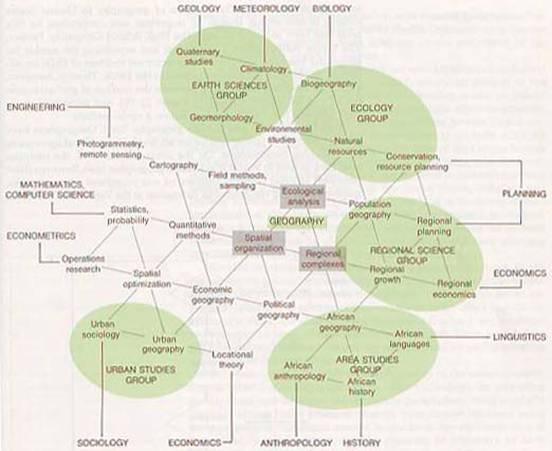
\includegraphics[width=.8\linewidth]{haggett1975_p587.jpg}
    \end{sidecaption}
  \end{figure}

Une exposition des influences de l'écologie, et des sciences naturelles (voir également le schéma \ref{fig:I_geoLink} proposé par \textcite[587]{Haggett1975}), que l'on retrouve beaucoup plus détaillée dans l'étude de l'écologiste et géomorphologue \textcite{Stoddart1967} parue dans \textit{Models in Geography} \autocite{Chorley1967}.

D'un point de vue opérationnel, et c'est aussi le cas dans les précédents ouvrages de ces pionniers, seules des tentatives probabilistes sont évoquées, via les travaux d'Hägerstrand, ou des économistes comme Curry. La méthode hypothético-déductive héritée des premiers géographes théoriciens semble encore être un implicite à la construction et l'évaluation des modèles. Les idées fortes de la systémique semblent avoir été entendues, mais paradoxalement il n'y a à cette période que très peu de références qui se rapportent aux techniques mathématiques ou informatiques capables d’opérationnaliser un tel système, et aucune application réelle \autocite[467-468]{Harvey1969}.

\paragraph{Les pionniers de l'opérationnalisation systémique en Europe}

La génération suivante de géographes va jouer un rôle important dans l'opérationnalisation de ces concepts au début des années 1970, tant en Angleterre, qu'en France où les géographes développent en collaboration avec des mathématiciens et physiciens les aptitudes nécessaires à la manipulation de ces nouvelles techniques computationnelles. \autocite{Pumain2002}

En Angleterre, la planification est issue d'une tradition qui date pour le \textit{Regional Planning and Policy} d'après 1920, et pour le \textit{Land use planning} d'après 1930. Ces activités sont rapidement construites en relations étroites avec les universitaires, les ingénieurs et les politiques publiques \autocites{Bennett2003}[727]{Davies1997}; un existant qui va être bouleversé courant des années 1960-70 par la rencontre conjointe des développements théoriques systémiques, des modèles de planification américains du milieu des années 1950, et d'une littérature qui anticipe la vague systémique. \autocites{Mcloughin1969}[4-8]{McLoughin1985}[253]{Batty1978}\Anote{anticipe_sys}. 

C'est sur ce substrat \autocite[253]{Batty1978} que des auteurs comme McLoughlin ou Chadwick publient dès le courant des années 1960 des états de l'art et des manuels d'applications qui vont rester pendant presque dix ans des références pour repenser la planification urbaine sous l'angle nouveau de la systémique \autocite[719]{Davies1997}. Une période qualifiée d'âge d'or pour la systémique anglaise, qui même si elle dure peu de temps \autocites[726-727]{Davies1997}{McLoughin1985}, marque toute une jeune génération de planificateurs qui vont être profondément influencés par ces approches \autocites[5-6]{Batty1976}[256]{Batty1978}; un constat alors en complet décalage avec la situation américaine, qui cristallise comme on a pu le voir dans la section \ref{ssec:crise_mutation} l'échec d'une décennie déjà révolue; les nouvelles pratiques, les nouveaux modèles ayant déjà exfiltrés les Etats-Unis, et la nouvelle génération bricolant déjà les meilleurs modèles en vue de les améliorer. C'est dans ce cadre notamment que le physicien et planificateur Wilson publie en 1970, le résultat de 4 ans de travaux pour concrétiser son idée, passer du paradigme newtonien au paradigme statistique boltzmanien pour revisiter dans une version spatiale et dynamique les modèles numériques classiques américains. \autocite{Wilson2010} Une approche qui va devenir avec le temps \enquote{l'école entropique} comme la nomme \textcite{Guermond1984}.

De cette plus jeune génération, à la croisée de ces inspirations, et tout à fait consciente des errements passés \footnote{Voir la conclusion de l'ouvrage de \textcite[357]{Batty1976} où l'auteur fait le point sur ces différentes positions, toutes abordées en filigrane dans ce livre synthèse : prédiction, explication, éducation }, on trouve des chercheurs maniant parfaitement ces techniques hybrides. Michael Batty est un bon exemple de chercheur représentatif de cette synthèse, qui pressent l'urgence de s'engouffrer dans une modélisation spatialisée plus dynamique \autocite{Batty1971,Batty1972} appuyée par les mathématiques des systèmes dynamiques, que cela soit au travers du vocabulaire de la dynamique des systèmes de Forrester, ou en suivant la toute nouvelle voie des modèles dérivés de l'école entropique de formation par Wilson.

%Le canal en écologie et géographie physique, dans la lignée des travaux de Chorley va également être particulièrement influent, avec l'avénement de modèle opérationel dérivée de la dynamique des populations de Lotka. \autocite{Batty 1971 ou 1972 ....}

%On trouve une analyse des premier essai systémique de Chorley analysé par le prisme des proposition du découpage de Parsons dans l'essai de Gregory.

Comme déjà évoqué brièvement à la fin de la section \ref{sssec:realite_neopositiviste}, les géographes français semblent au début des années 1970 peu réceptifs à l'épistémologie néo-positiviste, et beaucoup plus concentrés sur l'apport des nouvelles méthodes quantitatives dont la substance est révélée brutalement aux géographes français par la lecture (et ensuite la traduction) de manuels anglo-saxons qui condensent déjà 15 ans de pratiques et de découvertes \autocite[129]{Pumain2002}.

Concernant la diffusion du paradigme systémique \footnote{Le cas de la diffusion des méthodes quantitatives en France et de sa structruration en réseau de chercheurs a fait l'objet de la thèse de \textcite{Cuyala2014} dirigée par Marie-Claire Robic, Denise Pumain.}, les recherches d'Olivier Orain \autocite{Orain2001} sur ce sujet sont précieuses. L'auteur nous propose de lister dans les embranchements intellectuels d'une discipline en pleine reconstruction, les convergences et divergences autour de l'acceptation de concepts dont Orain estime qu'ils se sont diffusés dans la géographie française au début des années 1970. La diffusion de la GST de Bertalanffy est renforcée par la publication en 1973 de son ouvrage principal, alors même que l'activité conjointe (publications, traductions, organisations de conférences, d'ateliers) de différents passeurs ayant séjourné à l'étranger comme Bernard Marchand, Wanda Herzog, Henri Reymond, Jean-Bernard Racine, Sylvie Rimbert est soutenue par des acteurs \enquote{installés} comme Philippe Pinchemel, Paul Claval, Roger Brunet, Charles-Pierre Péguy \autocite{Pumain2002,Cauvin2007}, déjà au fait des publications et techniques pionnières anglo-saxonnes.

% NOTE CLEMENTINE et FDD ? il me semble que c’est une des premières thèses françaises dont « système » est le mot clé

Le mot \enquote{système} sort de l'ornière du sens commun et se pare de nouvelles significations, sous l'effet notamment d'ouvrages de référence comme celui de Jean-Bernard Racine et Henri Reymond  \textit{L’Analyse quantitative en géographie} (1973). Premier livre de géographie quantitative en France \autocite{Cauvin2007}, il développe un \enquote{ [...] vibrant plaidoyer pour le développement de concepts et de méthodologies systémistes dans une discipline qui selon eux, \enquote{ découvre que la notion de système lui était depuis longtemps familière, comme la prose à Monsieur Jourdain, et qu'il ne lui manquait que de la formaliser pour la rendre opérationnelle.}} \textcite{Orain2001}. Un appel qui sera entendu semble-t-il, pour Orain \autocite[23]{Orain2001} une des explications pour comprendre le succès connu par la systémique fin des années 1970 début 1980 est le fait que \enquote{[...] les Nouveaux Géographes [...] ont trouvé dans l’idée de système un appareil conceptuel permettant à la fois de penser l’intégration de l’hétérogène et d’apporter une légitimité scientifique à l’étude de la région}.

\Anotecontent{etat_artDPMC}{Sur cette thématique on trouve un excellent récit de Denise Pumain et Marie-Claire Robic \autocite{Pumain2002}, ou de Colette Cauvin \autocite{Cauvin2007}}

Dans l'établissement d'une géographie systémique, le Groupe Dupont qui naît à la suite de la conférence \enquote{révélatrice} donnée par Marchand en 1970 s'avère être un creuset important pour la formation, la réflexion, l'échange intra/inter-disciplinaire, et l'expérimentation autour de ces nouvelles techniques \autocites[2]{LeBerre1987}[125-128]{Pumain2002}. Une structure d'accueil que l'on imagine nécessaire pour fédérer des jeunes géographes plus habitués à l'étude monographique qu'à l'utilisation d'outils computationnels. Une période 1971-1975 marquée par la volonté des \enquote{nouveaux géographes} de se former aux mathématiques, une étape absolument nécessaire pour tirer profit par la suite de ces nouveaux formalismes statistiques et informatiques\Anote{etat_artDPMC}.

% REVUES ÉGALEMENT, voir Pumain2012 (quarante glorieuse de l'espace geographique)

En termes de réalisation, différentes écoles vont se créer autour d'objets géographiques ou de techniques parfois différentes, mais avec la même volonté de rendre compte de la complexité des systèmes géographiques en usant des outils mis à disposition par ce nouveau paradigme systémique. Car ce n'est pas tant l'évolution des concepts qui comptent pour certains géographes mais leur définition en termes opérationnels dans les modèles de simulation \autocite{Pumain2003}, seul moyen de confronter les données récoltées à ces nouvelles formes d'explications mathématiques. Bertalanffy entre autre l'avait déjà bien compris, mobilisées sans réelles démonstrations, les hypothèses intuitées, même lorsqu'elles sont quasi certaines, ne sont tout au mieux pour les autres chercheurs que des aides à la réflexion. Ainsi, et c'est avec une rapidité presque déconcertante, qu'il se raccroche aux premières découvertes de Prigogine en 1946 sur la physique des systèmes ouverts loin de l'équilibre pour appuyer ce qui jusque là ne sont que des intuitions dans sa théorie organismique, et qui forme le prélude à un projet systémique plus général (voir les annexes \ref{sec:annexe} pour plus de détails).

François Durand-Dastès et François Auriac sont des exemples de géographes qui développent dans leurs études toute la puissance heuristique des concepts systémiques et de leur traduction graphique pour décortiquer la complexité des systèmes géographiques.

Un autre groupe de géographes va pousser cette démarche heuristique encore plus loin, en lui donnant corps dans des modèles de simulation. C'est le cas par exemple du projet A.M.O.R.A.L ( Analyse systémique et MOdélisation des ALpes ) réalisé par des géographes et informaticiens grenoblois, qui est un des premiers résultats d'approche systémique spatialisé ayant pour objet d'étude une région française. Un double enjeu et une double expérience ici pour ces géographes, qui décident de tester la méthode systémique en la déroulant dans sa totalité, ce qui signifie également pour les étapes de réalisation de collaborer avec des informaticiens sur la partie système dynamique. \autocite{Guermond1984, LeBerre1987}

\Anotecontent{exp_amoral}{\enquote{[...] mes premières tentatives de modélisation systémique sont liées à un événement conjoncturel : la rencontre de chercheurs en informatique qui travaillaient, dans l'esprit de la dynamique de système de J.W. Forrester, à la mise au point d'un nouveau langage de simulation. Ils cherchaient à identifier, pour les formaliser, les types de problèmes soulevés par les recherches appliquées. Le groupe de géographes grenoblois avec lequel je travaillais, séduit par quelques ouvrages sur l'approche systémique, était tout prêt à faire l'investissement intellectuel pour tenter son expérimentation en géographie. C'est ainsi que nous avons choisi de modéliser la dynamique de l'emploi dans le système urbain de la région Rhône-Alpes.} \autocite[8]{LeBerre1987}}

Dans le cas du modèle A.M.O.R.A.L \autocite{Durand1983}, la démarche poursuivie est explicitement\Anote{exp_amoral} celle de l'expérimentation de l'\enquote{approche systèmes dynamiques} \autocite{Rosnay1975} à l'étude de la région, avec en tête des modélisateurs la réalisation de multiples objectifs, à la fois d'apprentissage, d'amélioration (prise en compte du spatial), de faisabilité, et d'applicabilité décisionnelle.

\Anotecontent{it_allen}{\enquote{Mais la rencontre opérationnelle - décisive -je l'ai faite en 1982, en allant à Créteil écouter - ne me demandez pas pourquoi - un colloque sur l'entropie dans lequel Peter Allen faisait un exposé sur les théories de l'auto-organisation. Dans cet exposé, il décrivait les modalités de changement de ces systèmes ouverts, loin de l'équilibre, qui connaissent de multiples fluctuations, dont certaines pouvaient s'amplifier et contribuer à modifier la structure du système tout autant que certaines bifurcations externes. C'était exactement ce que j'avais observé en étudiant les recensements périodiques de population, en poids économique, et transformaient leur structure qualitative sur le plan de leur portefeuille d'activités économiques, sur le plan de leur composition sociale, tout ceci en lien, bien sûr, avec des représentations que nous avions de cette dynamique des villes en terme d'images de marque, d'attractivité pour les migrations, etc.
Tout de suite j'ai été séduite par cette approche, et j'ai essayé d'expérimenter avec ces modèles mis au point par Peter Allen, qui à l'époque travaillait encore dans le laboratoire de Prigogine à Bruxelles avec Michèle Sanglier, mais plus particulièrement en direction d'applications à l'économie et à la géographie.[...] Il élaborait en effet des modèles spatialisés, notamment un modèle dynamique intra-urbaine ou intrarégionale [...]; il y'avait là beaucoup d'éléments de théories géographiques qui étaient mis dans un modèle de simulation qui permettait d'expérimenter les effets de ces briques théoriques et de les confronter à des observations.} \autocite[153-154]{Mathieu2014}}

\Anotecontent{appli_allen}{\enquote{Tous ces auteurs se sont toutefois heurtés à l'insuffisante prise en compte de la dimension spatiale dans cette famille de modèles. Aussi, des travaux application et élaboration de \textit{modèles urbains} qui soient à la fois \textit{dynamiques et spatiaux} sont en cours. Un modèle comme celui de P.Allen (1978), fondé sur l'analogie des structures dissipatives en physique, permet de simuler le développement d'une ville en tenant compte des interactions non linéaires (avec effets d'amplification ou de saturation), spatiales ou non spatiales, qui commandent la redistribution des emplois et des populations entre les différents quartiers. Il permet de prévoir diverses configurations possibles dans le futur à partir d'une histoire donnée. Ce modèle a été appliqué à la simulation du développement de l'agglomération de Rouen (Ozan et al. 1983)} \autocite{Pumain1983}}

\Anotecontent{auto_definition}{Un autre concept important est introduit par Ashby dans le mouvement Cybernétique, l'introduction du mot \enquote{auto} amorcent un virage réflexif propre à la seconde Cybernétique, pilotée par William Ross Ashby et Von Foerster. Si le concept en lui-même est largement intuité dans les thèses de Goethe et Bertalanffy \autocite[102]{Pouvreau2013} dans sa traduction biologique, on retrouve un concept équivalent dans le \enquote{order-from-noise} de Von Foerster, et \enquote{order-from-fluctuation} dans la physique de Prigogine.}

De façon parallèle, Denise Pumain\Anote{pumain_decouverte}, aidée par d'autres géographes comme Lena Sanders et Thérèse Saint-Julien participe dès 1980 d'un courant \autocites{Pumain1983, Pumain1984, Pumain1989} qui vise l'application des modèles de simulation à l'étude des villes et des systèmes de villes, et cela sur des bases beaucoup plus empiriques, devançant ici les diverses tentatives des anglo-saxons faites jusqu'à alors \autocite[99-100]{Pumain1989}. Mais dans le cas de cette équipe, si l’intérêt porté à la dynamique des systèmes de Forrester est là aussi évidente \autocites{Pumain1983, Pumain1984}, le chemin emprunté sur le plan opérationnel va semble-t-il rapidement diverger de celui suivi par l'équipe AMORAL. Avec la révélation d'une opérationnalisation possible par l'usage de la \enquote{dynamique des systèmes}, les géographes peuvent donc aller plus loin dans l'exploration du support mathématique sous-jacent, et ainsi mesurer dans l'évolution des \enquote{systèmes dynamiques} vue comme discipline mathématique la possibilité de construire des modèles encore plus proches d'une évolution réelle des objets géographiques. Ainsi, là où le modèle AMORAL cherche à spatialiser l'approche systémique qui dérive de la dynamique des systèmes de Forrester, les frustrations de l'équipe de Denise Pumain face à leurs propres études passées sur la dynamique des villes vont les amener à explorer un tout autre chemin en termes d'opérationnalisation.

Ainsi, et c'est dans ce contexte de frustration par rapport aux approches existantes\Anote{appli_allen} que se produit au début des années 1980 cette découverte contingente du concept d'auto-organisation, dont la réalité opérationnelle exprimée dans des modèles mathématiques exposés par les physiciens de l'école de Bruxelles semble offrir tout à coup toutes les garanties pour former des modèles de simulations beaucoup plus réalistes de l'évolution des villes\Anote{auto_definition} \autocite[350]{Pumain1998a}. La possibilité également de concrétiser les intuitions systémiques des pionniers qui envisagent très tôt la nécessité de penser les systèmes urbains comme des systèmes ouverts, comme celle évoquée en 1964 par \textcite{Berry1964a} et son article \enquote{Cities as systems within systems of cities}. La rencontre de Denise Pumain avec le chimiste Peter Allen en 1982 à Créteil\Anote{it_allen} est l'expression même de cette contingence, qui va donner par la suite naissance à de multiples modèles et collaborations avec les physiciens de l'école des \enquote{structures dissipatives} de Bruxelles d'abord, puis de l'école de la \enquote{Synergétique} de Haken ensuite \autocites[27]{Pumain2003}{Pumain1982b, Mathieu2014,Sanders1984, Sanders1992}.

A une phase cybernétique déjà révélatrice de concepts systémiques tout à fait nouveaux pour penser la causalité en géographie, les géographes découvrent par extension la richesse et la pluri-disciplinarité des systèmes dynamiques, alors en pleine évolution. Pourtant déjà évoquées par Poincarré, et étudiées par différents mathématiciens dès le début du siècle, la diffusion des théories de la bifurcation n'atteint son point culminant que courant des années 1970. La conférence de New York en 1977 qui se tient sur ce sujet est selon \textcite{Dahan1991} un marqueur singulier de cette dynamique convergente qui pousse de multiples disciplines (physiques, chimiques, biologiques, etc. ) à se rencontrer, non seulement pour évoquer et mettre en commun leurs questionnements et réflexions sur la nature instable des phénomènes, mais aussi pour venir chercher dans cette conférence de nouveaux outils mathématiques adaptés à sa formalisation. L'apparition de \enquote{systèmes frontières} comme par exemple le système de \enquote{Rayleigh-Bénard} va constituer en devenant un objet d'étude partagé, un formidable point de rencontre entre les points de vue originaux des physiciens développant des appareils de mesures, physiciens, thermodynamiciens, hydrodynamiciens. Mais \enquote{l’adoption d’une approche de type système dynamique pour le comprendre ne constitue pas le moteur principal de la convergence. En fait, l’adoption du langage des systèmes dynamiques est ici plutôt la conséquence d’un désir de convergence manifesté par divers groupes de scientifiques} \textcite{Dahan1991}.

%\begin{framewithtitle}{Les théories de la bifurcation}

	% \begin{figure}[h]
	% \begin{sidecaption}[fortoc]{Un exemple de bifurcation Pitchfork}[fig:S_BPF]
	%   \centering
	%  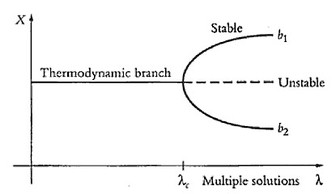
\includegraphics[width=.7\linewidth]{pitchfork_bifurcation.jpeg}
	%   \end{sidecaption}
	% \end{figure}

%\end{framewithtitle}

%La théorie des catastrophe de René Thom, bien connus des géographes, est un cas particulier de la théorie des bifurcations.

Elle offre un support aux découvertes des physiciens engagés depuis les années 1930 dans les travaux sur les processus physiques et chimiques des systèmes ouverts éloignés de l'équilibre, qui observent dans la trajectoire d'évolution de ces systèmes l'apparition de zones d'instabilité, causées par la modification en interne des fluctuations ou en réponse à des variations des échanges externes avec l'environnement.

Si certaines conditions d'une auto-organisation avait déjà été avancées dans une preuve matérielle (Homéostat) et un support théorique (Loi de la Variété requise) dans les travaux par exemple d'Ashby \autocite[800-801]{Pouvreau2013}, les physico-chimistes comme Prigogine ou Haken, en montrant qu'il était possible dans certains systèmes physiques (laser) ou chimiques (structures dissipatives) chaotiques, de voir apparaître au cours des bifurcations de nouveaux équilibres dynamiques caractérisés par l'émergence de structures ordonnées de niveau supérieur issues de l'organisation des interactions à un niveau inférieur, ont fourni une évolution du substrat théorique et mathématique solide du concept d'auto-organisation sur lequel peuvent s'appuyer les chercheurs pour expérimenter des analogies dans les systèmes sociaux ou biologiques.

%l'approche d'un point de bifurcation correspondant à l'émergence d'une structure lié à une variation de paramètres dans un processus chaotique/instable décrivant une trajectoire stable entraînant l'émergence imprévisible d'un nouvel état ordonné/stable, dont la structure est maintenu par consommation d'énergie extérieure.

%dévoile de nouvelle perspectives pour penser l’emboîtement et les relation opérant entre les différentes échelles d'observations (voir Annexe A).

%La matérialisation d'un modèle urbain, même théorique, ouvre la voie à des développements qui ouvre la voie à une nouvelle forme de causalité.

La translation de ces concepts sera opérée avec précaution par Pumain et Sanders, et amène une réflexion sur l'évolution des objets géographiques dont on trouve une plus grande explication dans les textes de \textcite{Pumain1982b, Pumain1989}.

%L'apport du paradigme systémique, et de son opérationnalisation

%Sous détermination
%Equifinalité

%Les deux approches sont clairement supportés par une double dialectique dans l'utilisation des outils statistiques et systémique, et dans la déduction et l'induction. (hum)

%\enquote{Tenant pour légitime de traiter les êtres vivants et leurs associations comme des systèmes physiques, Lotka insistait toutefois sur le fait qu’il s’agit de « systèmes ouverts » aux flux de matière et d’énergie (ainsi que Raymond Defay (en 1929) et Bertalanffy (en 1932) les qualifièrent plus tard), capables d’échapper à l’équilibre thermodynamique défini par un maximum d’entropie promis aux systèmes fermés par le Second Principe, et d’évoluer vers une structuration croissante.}\autocite{Pouvreau2013}

%\autocite{Pouvreau2013} sa théorie arrive à maturation : \enquote{Un système organique quelconque n'est essentiellement rien d'autre qu'un ordre hiérarchique de processus qui se tiennent mutuellement en équilibre de flux [...] Un organisme vivant est un ordre hiérarchique de systèmes ouverts, qui se maintient sur la base de ses conditions systémiques par un changement de ses composants}

%L'apport de ces techniques, est un vrai écho à ce que disait Le Berre; Sanders et Pumain. D'une part les outils permettent d'ouvrir de nouvelles perspectives de réflexions, et ceux ci s’intègrent dans une chaîne de raisonnement qui s'organisent non pas de façon linéaire mais dans dialogue ou ce sont les usages, les questions, les objets à étudier qui guident l'utilisation et l'amélioration de ces outils.

% Partant de Pumain2002 Pumain2003, la première remise en cause de la causalité est le concept de non linéarité des interactions,

% Relation de variété entre les niveau de hierarchie, augmentation du degré de variété, ce qui va avec le concept équifinalité, un peu different du concept de sous détermination...
% Plusieurs débats qui vont venir agiter la problématique de la construction des modèles, et surtout de leur validation.
% Forrester causalité, construction des modèles, sous détermination
% Auto-organisation problématique de

%Dans cette partie, il s'agit donc de mettre en avant ces débats philosophiques en les reliant aux nouvelles problématiques de construction des modèles tel qu'elle apparaissent aux tournant des années 1970.

%Quel sont les moyens offerts de cette validation ? Existe-il une spécificité de cette validation dans son application en science sociale, et plus spécifiquement en géographie, et qui n'est pas prise en compte dans ces définitions ?

%Plusieurs débats viennent encadrer à la fois la validation mais aussi le support opérationel de cette validation. Autrement dit, comment détermine t on si un modèle est validé ou pas, et quel est la nature de cette validation opère sur un substrat particulier, qui en fait une expérience sur le réel de second ordre.

%IMPORTANT : Necessite d'avoir une validation pour les sciences sociales.

\subsubsection{L'impact du programme de Forrester dans le débat sur la Validation}
\label{sssec:forrester_impact}

Deux dates sont à retenir dans le programme forresterien, la publication du \enquote{programme} d'\textit{Industrial Dynamics} en 1961; l'aboutissement des recherches démarrées en 1956 au MIT, et dans un deuxième temps en 1969 la proposition de translation de ce programme à l'étude plus large des systèmes sociaux, avec l'expérience du modèle \textit{Urban Dynamics}.

Pourquoi parle-t-on de programme ici, et non pas seulement de modèle ?

L'apport de Forrester ne se résume pas en réalité au seul nouveau langage de programmation DYNAMO, celui-ci propose aussi avec une méthodologie et un vocabulaire graphique. Trois éléments qui une fois réunis permettent de dériver opérationnellement les concepts clefs du projet systémique dans un modèle de simulation dynamique, ce qui en fait un outil d'intérêt général non seulement pour la géographie, mais pour toute les autres disciplines confondues (biologie, économie, sciences humaines, etc.) \autocite{Rosnay1975}

\paragraph{Urban Dynamics, un révélateur des nouveaux usages pour la construction et la validation des modèles ?}
\label{p:urbanDyn_revelateur}

Provenant d'une toute autre inspiration et construit selon un tout autre patron que les modèles urbains réalisés jusqu'à la fin des années 1970, le modèle \textit{Urban Dynamics} de \textcite{Forrester1969} fait une entrée très remarquée dans le milieu des \textit{policies}. Celui-ci met en jeu une ville abstraite et isolée, non-spatialisée, où interagissent de façon a-spatialisée de multiples mécanismes regroupés par activités et organisés en chaîne causale. Le modèle ne fait appel à aucune donnée pour calibrer ou vérifier les sorties générées, et à ce titre il ne peut pas être considéré comme un modèle décisionnel sérieux pour les \textit{policy analysis} de l'époque \autocite{Lee1973}. Soumis à une très forte médiatisation, les critiques sur le modèle se font parfois vives tant du côté des citoyens \autocites{Forrester1989, Forrester2007} que des universitaires géographes \autocites{Tobler1970a, Berry1970b, Batty1971, Batty1976} .

Il est vrai que d'un point de vue purement géographique et même technique, le modèle \textit{Urban Dynamics} n'introduit pas tant d'originalité par rapport aux éléments acquis par la rencontre entre la vision d'Hägerstrand et les pionniers universitaires 10 ans auparavant. On se remémorera à ce sujet la citation de \textcite{Morril2005} qui résume très bien l'importance de cette convergence, ici en quatre grands points : \foreignquote{english}{First was the introduction (at least at the geography) of the idea of spatial and time-processes, that geographic development over time could be understood and modeled; second was the particular processes of spatial diffusion; third was the technique of Monte-Carlo simulation; and fourth was the idea that individual behavior, not just that of large groups, could be modelled}. Ainsi après tout, les premiers modèles de simulation qui incorporent la dimension temporelle, stochastique, dans le premier langage Fortran, sont datés d'avant 1965, et dépassent en bien des aspects la vision a-spatiale proposée par Forrester.

L'étude des processus de diffusion abordés dans les simulations pionnières suppose assez naturellement que les géographes intègrent le temps dans leurs analyses, et il a été vu précédemment que la simulation est un formidable outil d'expérimentation pour la projection et l'évaluation dans le temps de multiples hypothèses (section \ref{ssec:labo_virtuelle}). En dehors de quelques exceptions\Anote{batty_temps}, pourquoi cette approche percole-t-elle aussi lentement dans l'analyse des systèmes urbains en géographie, où la simulation numérique est mobilisée à la même période sans pourtant y intégrer la dimension temporelle? Sorte de principe de parcimonie poussé à l'extrême, où l'absence du temps si elle permet de simplifier l'analyse, mène toutefois à des prédictions absurdes ou impossibles, qui ne tiennent pas compte des évolutions de structures sur lesquelles s'appuient les interactions dans les systèmes urbains. Le constat d'une forme d'auto-censure de la discipline pour laquelle \textcite[296-297]{Batty1976} nous donne quelques pistes de compréhension :

\foreignblockquote{english}[{\cite[296-297]{Batty1976}}]{There are, however, good reasons why the comparative static approach has been widely applied. The status of theory in urban economic and geographic systems with regard to time is almost non-existent. [...] Yet there are severe problems in trying to develop dynamic theory, two of which are worthy of some discussion.[...]

Perhaps the major problem concerns the ability to observe or monitor the urban system. Unlike the physical sciences in which the effect of critical variables on the system of interest can be isolated in the laboratory, such a search for cause and effect is practically impossible in social systems. Thus, there are many instances when it is difficult, if not impossible, to disentangle one cause from another in the changing behaviour of such systems. This is a fundamental limitation which is referred to here as the \textbf{observational dilemma}.

A second problem concerns that hoary perennial data. [...] data are often difficult to assemble for one cross-section in time, and the collection of time series data is usually a formidable and sometimes infeasible undertaking. Furthermore, such data often become less consistent and sparser as earlier time periods are needed and, frequently, the time periods between points at which data have been collected, are too large to be useful for dynamic modelling}

%%NOTE CLEMENTINE à ce propos, pour préparer mon entretien skype, j’ai regardé plein de vidéos récentes de Batty et de son accent bien anglais. Y’en avait une je sais plus où assez cool qui répond à cette citation de 40ans. En gros, il parle des Big Data et de la façon dont leur structure (non-exhaustif, irrégulières dans le temps mais dans un temps plus ou moins continu etc.) change qualitativement les analyses. C’est pas juste plus de données mais données différentes et questions à poser d’un autre ordre. juste comme ça.

Si on revient au modèle \textit{Urban Dynamics} de Forrester, celui-ci pourrait après tout passer pour une nouvelle tentative parmi d'autres, car comme Tobler le fait remarquer dans sa critique du modèle : \foreignquote{english}{In other words, it is a classical non-linear deterministic equilibrium model, but of great complexity.} \textcite{Tobler1970a}

Pourquoi Batty en fait-il alors régulièrement un modèle pivot dans son argumentation dans l'évolution de la discipline \textcite{Batty1971, Batty1976, Batty2001, Batty2008}, et pourquoi celui-ci a-t-il autant attiré l'attention dans le monde académique ?

Sur ce deuxième point, on a déjà donné un élément de la réponse dans l'introduction de cette partie. Forrester vient ici avec plus qu'un modèle, il vient avec un programme \autocite{Forrester1961} qui embrasse littéralement les concepts de la systémique dans sa branche cybernétique \autocite{Berry1970b}, ce qui permet d'apporter, avec l'intégration du temps, un tout nouveau point de vue sur la planification et la mise en place des politiques publiques. Ainsi malgré ses défauts, \foreignquote{english}{[...] the model is an illustrative first attempt that points the way for others. It is the direction that is important, and Forrester's book may yet prove to be one of the important signposts in the attempt to deal more sensitively and effectively with urban problems.} \autocite{Berry1970b}

L'autre point fort du programme de Forrester est la possibilité d'opérationnaliser des concepts de la systémique tout en maintenant un coût d'accès à la simulation qui paraît plus adapté au monde académique des sciences humaines et sociales, et cela entre autre par la mise en place d'une triple entrée en la matière : informatique avec DYNAMO (un langage déjà adapté/simplifié pour réaliser des simulations), mathématique avec les systèmes dynamiques, et graphique avec les diagrammes de \foreignquote{english}{stock and flow}.

%NOTE CLEMENTINE une figure-exemple ?

Pour ces deux raisons, on comprendra donc ici que le monde académique soit plus intéressé par les nouvelles possibilités offertes par l'environnement support du modèle que par le modèle en lui-même, qui restera chez les géographes un cas d'utilisation finalement assez peu repris dans des travaux ultérieurs chez les anglo-saxons \autocite[308]{Batty1976}, et chez les français. %\hl{(ref)}

Ainsi, ce n'est pas tant sur les aspects temporels que \textcite{Batty2001} en font un modèle en rupture avec son passé, mais sur le débat qu'il soulève du point de vue de la validation.

\foreignblockquote{english}[\cite{Batty2001}]{Perhaps the clearest model which broke from this tradition and which illustrated distinctly the problems posed by the current generation of models based on complexity was Forrester’s (1969) Urban Dynamics model.} 

Pour comprendre la position de Forrester sur ce point il faut s'intéresser d'un peu plus près à sa vision de la modélisation et à l'utilisation qu'il souhaite en faire dans le cadre des politiques publiques. Pour lui, le problème n'est pas tant les données\Anote{batty_donnees}, que l'on finit toujours par obtenir, \foreignquote{english}{ [...] but rather inability to perceive the consequences of information we already possess.}\Anote{batty_ok}. Les décideurs politiques se font une image de la réalité - modèle mental -, or souvent cette image serait trompeuse, ce qui amèneraient à la faillite des politiques ainsi menées. Pour \textcite{Forrester1971}, l'usage de modèle de simulation permet de re-projeter ces modèles mentaux faillibles sur des modèles informatiques dont la construction nécessite la formulation d'hypothèses de façon plus explicite, plus compréhensible, et sur lequel il est possible de dialoguer de façon plus constructive. Il n'est plus question de choisir en fonction d'un seul scénario, mais de plusieurs, avec la possibilité de projeter et d'évaluer dans le temps les conséquences de dynamiques complexes sur un système simplifié envers un objectif donné, et cela avec la garantie d'une fiabilité bien au-delà de ce que le seul esprit humain ne pourrait espérer. Avec souvent un résultat sans appel, \foreignquote{english}{[...] behavior is different from what people have assumed.} Un comportement qu'il arrive à démontrer par le jeu des rétro-actions des mécanismes de son modèle \textit{Urban Dynamics}, qui illustre les effets tout à fait contre-intuitifs de certaines politiques publiques.

Comme sous-entendu dans le paragraphe précédent, en réalité on comprend beaucoup mieux la démarche de Forrester dès lors qu'on comprend qu'il n'a jamais été question ici de faire un modèle opérationel, comme le sous-tend aussi \autocite{Batty2001} : \foreignquote{english}{It might be, as was argued at the time, that the purpose of this model was to raise the level of debate about the inner city. It was not to provide an operational simulation. It was to foster discussion about possible policy issues.}

Ce qui explique entre autre la curiosité ou la perplexité des planificateurs \autocite{Lee1973} ayant investi des millions de dollars sur plusieurs dizaines d'années dans la construction de modèles s'appuyant sur des récoltes de données à la fois coûteuses et fastidieuses.

Le support de cette discussion passe par l'établissement d'un graphe causal représentatif d'un système clos dans sa définition, mais ouvert dans ses échanges vers l'extérieur, dont les éléments et les interactions entre les éléments sont au centre du débat. %\hl{description graphe forrester}

Mais en acceptant cela, et compte tenu de l'\textit{observational dilemna} défini par Batty, le modèle de simulation devient dans l'établissement de sa structure causale la projection d'une histoire, d'un point de vue, ici celui de Forrester et de ses collaborateurs. Dès lors l'attention ne se porte plus seulement sur le résultat, mais aussi sur le bien fondé des hypothèses mobilisées par Forrester pour établir ce résultat.

Il y a un certain paradoxe à voir dans cette situation, car si effectivement Forrester donne à voir avec ce graphe causal son raisonnement, contrairement à de nombreux modèles urbains autrefois qualifiés de \enquote{boîte noires}, c'est précisément sur ce point qu'il va se faire attaquer. Les critiques des géographes ne manquent pas alors de rappeler qu'en dehors de l'a-spatialité et l'isolation du modèle, celui-ci n'a intégré absolument aucune référence aux théories urbaines dans son travail. Outre, le fait que ce n'est pas très \textit{fair play} de sa part pour les universitaires travaillant sur ce sujet depuis 10 ans, cet isolement relatif (Forrester mobilisera d'autres sources) se traduit dans le modèle par la mise en oeuvre de centaines d'hypothèses (400 équations, 300 variables et paramètres \autocite[63]{Pumain1989}) qui s'avèrent pour la plupart difficilement justifiables ou testables de façon empirique \autocite[307]{Batty1976}.

La critique de \textcite{Tobler1970a} sur ce point est explicite, \textit{Urban Dynamics}

\foreignblockquote{english}[\cite{Tobler1970a}]{[...] is a classical non-linear deterministic equilibrium model, but of great complexity. Herein lies its importance for it is rather grandiosely conceived. [...] Not only the values of the parameters, but also which variables are chosen for consideration and how they are interconnected, are critical. [...] the danger is that his model has not really been tested empirically, thus the policy implications may be wrong, and the model - because of its complexity - is extremely difficult to test. A very careful study of the many assumptions of the model are required. Also required are more competing models, thus the book’s greatest achievement may be the competition which it stimulates.}

Dernier point, peut-être le plus préjudiciable à la démarche vantée par Forrester, est la règle qu'il donne pour définir le choix des hypothèses dans un graphe de causalité :

\foreignblockquote{english}[\cites{Forrester1968b, Richardson2011}]{Formulating a model of a system should start from the question \enquote{Where is the boundary, that encompasses the smallest number of components, within which the dynamic behavior under study is generated?} [...] In concept a feedback system is a closed system. Its dynamic behavior arises within its internal structure. Any action which is essential to the behavior of the model being investigated must be included inside the system boundary.}

Sachant cela, et le fait que différentes équipes arrivent à reproduire la même dynamique finale avec la mise en œuvre de modèles beaucoup plus parcimonieux, l'effet est catastrophique pour l'argumentation de Forrester ! Lee\Anote{lee_forrester} et Batty\Anote{batty_forrester} font référence en particulier aux travaux de \autocite{Stonebraker1972}.

Ainsi quand \textcite{Batty2001} parlent du modèle de Forrester comme ayant polarisé le débat, ce n'est pas pour éclairer sa réussite dans cette lourde tâche de fabriquer un modèle crédible sur le plan des hypothèses du point de vue d'une communauté des géographes, car sur ce point l'échec semble complet. Son approche légitime par contre indirectement une construction de modèles complexes qui n'impliquent pas forcément une vérification stricte par les données (sur les hypothèses, mais aussi en sortie). Une \foreignquote{english}{Forrester strategy}, identifiée par \textcite[7-8]{Batty2001} comme le retranchement des modélisateurs dans une rhétorique masquant en réalité une absence de volonté ou une incapacité (technique, méthodologique, philosophique) à justifier de la chaîne causale mise en place dans le modèle, celui-ci ne servant plus qu'à animer ou illustrer un débat où clairement la neutralité scientifique n'est plus une priorité.

Le débat s'organise alors autour d'un problème qui parait insoluble, avec d'un côté cette nécessité - pour être crédible d'un point de vue scientifique - de pouvoir justifier empiriquement le réseau d'hypothèses mobilisées dans notre modèle complexe, et d'un autre côté l'impossibilité de pouvoir toutes les justifier du fait de l'\textit{observational dilemna} et de la difficulté/impossibilité d'obtenir des données dans bon nombre de disciplines en sciences sociales. Un paradoxe d'autant plus renforcé quand on sait que la simulation est justement mobilisée dans certaines disciplines pour mettre en valeur des comportements du système jugés inobservables dans la réalité, soit parce que qu'ils ne peuvent pas être isolés, soit parce qu'ils ont tout simplement disparus.

Remis dans son contexte, et bien qu'elle soit affaiblie justement par le choix d'une cible plus politique (une réussite pour avoir montré qu'il y a des phénomènes contre-intuitifs) que scientifique (un échec du point de vue des hypothèses injectées), la thèse de Forrester a le mérite de se positionner comme une validation avant tout dépendante d'un contexte. Un point de vue qui peut paraître évident aujourd'hui mais qui va pour l'époque se heurter à une vision de la validation héritée de l'économie beaucoup plus rigide sur ce point de vue, et dont nous allons voir qu'elle est de toute façon inadaptée à la validation des modèles en sciences sociales.

%Car comment valider un modèle qui ne s'appuie sur aucune données autres que des valeurs de paramètres, et qui évoque des conclusions sans avoir été calibré au préalable ? Comment discuter des résultats de cette longue suite d'hypothèses reliés les uns aux autres par des interaction complexes, difficile ou impossible à vérifier empiriquement ? On retrouve là les deux points évoqués par Batty pour justifier du retard dans l'intégration du temps dans les modèles urbains, sur lesquels Forrester est clairement mis en difficulté.

\paragraph{Forrester, un acteur du débat entre Validation Objectiviste et Relativiste}
\label{p:confrontation_approches}

Avant même la publication de \textit{Urban Dynamics}, c'est déjà sa première publication \textit{Industrial Dynamics} qui doit faire face à plusieurs critiques extrêmement vives de la part d'opposants à sa méthode de validation \autocite{Barlas1990}. Ces derniers affichent alors des vues plus proches d'une autre méthode de validation, beaucoup plus rigide, telle qu'elle est proposée par Naylor; un des pionniers sur cette question et dont la vision a une large influence dans la littérature de la validation courant des années 1960-1970. Un postulat qui se base à la fois sur des commentaires de chercheurs comme \autocite[1088]{Kleindorfer1998} \autocite{Nance2002}, mais également d'une constatation faite dans la lecture des ouvrages collectifs \autocite{Guetzkow1972}, où Naylor apparaît souvent comme la voix référente sur cette question.

\Anotecontent{banks}{Jerry Banks dans son livre régulièrement réédité \textit{Discrete-Event System Simulation} propose toujours aux lecteurs de valider leur modèle en s'appuyant sur une version synthétique et modernisée de l'approche proposée par Naylor}

Bien que sa méthodologie soit la plus souvent citée dans le domaine de la \textit{V\&V} comme une \enquote{méthodologie historique} \autocite{Sargent2010}, celle-ci reste pourtant tout à fait influente et opérationnelle de par sa présence régulière dans des ouvrages d'ingénierie généraliste\Anote{banks}.

Pour \textcite{Kleindorfer1998}, cette vision historique de la validation telle qu'elle a été définie par Naylor est la cause encore aujourd'hui de nombreux malentendus et critiques qui touchent la validation de modèles. A ce titre, et dans le but de faire progresser ce débat, \textcite{Kleindorfer1998} se positionne comme arbitre entre d'un côté l'\enquote{objectivisme} représenté par Naylor, et de l'autre côté la vision opposée plus \enquote{relativiste} représentée par Barlas et Carpenter, eux aussi extrêmement critiques envers la vision de Naylor.

Une fois remise dans son contexte, la méthodologie proposée par Naylor est au premier abord particulièrement intéressante; pas seulement car c'est la première fois que l'on s'intéresse à cette problématique, mais aussi parce que celle-ci aborde cette réflexion en y intégrant spontanément le point de vue de la philosophie des sciences. Mais il ne s'arrête pas là, car c'est avec une certaine ouverture d'esprit qu'il insiste ensuite auprès du lecteur sur la nécessité d'une approche éclectique de cette question de la validation; celle-ci n'étant pas pour lui l'histoire d'un seul dogme forcément incomplet, mais d'un faisceau d'approches résolument complémentaires. Il retient trois approches qu'il regroupe par ordre d'application dans une méthode nommée \textit{Multi Stage Validation} et qui contient : le rationalisme cartésien, l'empirisme, et la \textit{positive economics} de Friedman.

Seulement, après lecture et analyse de cet article, on s'aperçoit que les trois points de vue qu'il présente se rapportent à une vision de la validation en réalité assez rigide, comme en témoigne cette citation tirée de l'article de \textcite{Naylor1967} : \foreignblockquote{english}{To verify or validate any kind of model (e.g management science models) means to prove the model to be true. But to prove that a model is \enquote{true} implies (1) that we have established a set of criteria for differentiating between those models which are \enquote{true} and those which are not \enquote{ true }, and (2) that we have the possibility to apply these criteria to any given models}

Pour \textcite{Barlas1990, Barlas1996}, il existe deux camps philosophiques opposés, et pour lui Naylor fait clairement partie de la première école :

\foreignblockquote{english}[\cite{Barlas1990}]{The traditional reductionist logica1 positivist school (including empiricism, rationalism, verificationism and the “strong” falsificationism) would see a valid model as an objective representation of a real system. The model can be either “correct” or “incorrect”; once the model confronts the empirical facts, its truth or falsehood would be automatically revealed. In this philosophy, validity is seen as a matter of accuracy, rather than usefulness. The opposing school (including more recent relativistic, holistic and pragmatist philosophies), in contrast, would see a valid model as one of many possible ways of describing a real situation. \enquote{No particular representation is superior to others in any absolute sense, although one could prove to be more effective. No model can claim absolute objectivity, for every model carries in it the modeler’s worldview. Models are not true or false, but lie on a continuum of usefulness}.}

\textcite{Barlas1990} font de Forrester le premier défenseur d'une validation plus en accord avec la deuxième école, une méthode selon lui plus adaptée à l'explication de processus complexes, comme en témoigne ces quelques extraits tirés de son article :

\foreignblockquote{english}[\cite{Barlas1990}]{The first exposition of the system dynamics paradigm as it relates to model validity was given in Chapter 13 of Industrial Dynamics (1961) by Jay Forrester. [...]

Forrester also criticizes the illusion that using fixed statistical significance levels brings objectivity to the validation procedure. [...]

He makes the stronger claim that \foreignquote{english}{the validity of a model should not be separated from the validity and the feasibility of the goals themselves.} Since reaching an agreement on the feasibility of the goals cannot be achieved through a formal algorithmic process, validation becomes very much a matter of social discussion. [...]

Another nontraditional view of Forrester is his willingness to accept \foreignquote{english}{qualitative} model validation. He argues that a negative attitude toward qualitative validation procedures is not justifiable, since \foreignquote{english}{a preponderant amount of human knowledge is in nonquantitative form} \autocite[128]{Forrester1961}. [...]

Finally, Forrester sees explanatory power as being at least as important as predictive power in model validation. Forrester’s views on model validity correspond to the relativist/holistic philosophy of science. }

En ce sens il prend le contre-pied de la dernière méthode qui clôt la \textit{multistage validation} de Naylor. La \textit{positive economics} dictée par Friedman, une forme d'instrumentalisme, est complétée par les deux méthodes précédentes (empirisme, rationalisme) pour assurer que la validation du modèle, et des hypothèses qu'il contient, est bien dirigée en priorité par la prédiction : \foreignquote{english}{ Hence the final decision concerning the validity of the model must be based on its predictions.} \autocite[97]{Naylor1967} Or il a été montré précédemment (voir \ref{p:echec_critiques} que c'est bien un des points reprochés par une partie des géographes radicaux que de voir s'aligner une partie des géographes (volontairement ou involontairement) sur une forme d'instrumentalisme, hérité de l'économie, et cela même appuyé par une position empiriste pour la validation des hypothèses.

Clairement le paradigme systémique permet d'échapper à ce discrédit par l'intégration dans les modèles géographiques d'une réflexion à la fois multi-échelle, et multi-temporelle \autocite{Dastes2001a} dont la discrétisation en une multitude de points d’arrêt pertinents constitue il me semble un appel implicite à l'étude inter-disciplinaire des objets géographiques, et dont la collection est toujours abordée en fonction de la question qui est posée. Ainsi l'étude de l'évolution comparée des systèmes de villes dans le temps long, ou l'étude des mobilités des individus liés à l'attribution des cartes scolaires sont deux exemples de sujet dont les composantes complexes ne peuvent être abordées sans faire appel à l'expertise comparée de sociologues, d'archéologues, d'économistes, etc. qui disposent pour le même objet (l'individu, la ville) de points de vue prompts à enrichir les modèles d'une hétérogénéité permise par la systémique.

Autre point qui semble en divergence avec les pratiques des géographes, la position empiriste de Naylor implique de limiter le choix d'hypothèses mobilisées dans les modèles aux seules qui peuvent être validées par des données : \foreignblockquote{english}[\cite{Naylor1967}]{A simulation model, the validity of which has not been ascertained by empirical observation, may prove to be of interest for expository or pedagogical purposes, but such a model contributes nothing to the understanding of the system being simulated}

Une vision radicale qui se heurte au problème de l'induction comme il avait déjà été évoqué pour les positivistes logiques ( section \ref{p:critique_debat} ), l'accumulation de confirmation n'étant en aucun cas une condition suffisante à la validation d'une hypothèse.

De plus, toutes les disciplines n'ont pas la possibilité de disposer de données utilisables pour vérification des hypothèses, et d'autre part la collecte et la structuration des données tient d'un processus qui contient là aussi une part de choix qui rend discutable la mise en place d'un seul jeu d'observation pour validation d'une seule et même hypothèse.

Enfin, cette vision est de toute façon peu compatible avec une étude de la complexité des systèmes sociaux (\foreignquote{english}{observational dilemna} de Batty), car comment rendre compte par une récolte de données de processus dont on sait d'une part que la perception et donc l'établissement de mesure est subjective (voir point précédent) et d'autre part que ces processus ne peuvent être réduits à leur seule composante du fait de leur intrication dans un réseau complexe d'interaction (le tout est plus que la somme des parties).

%Cela pour plusieurs raisons qui tiennent à la construction des connaissances dans la simulation des systèmes sociaux, dont on verra par la suite qu'elle ne peut que difficilement être similaire à la construction des connaissances dans les sciences naturelles.

%La où la validation proposée par Naylor ne se réalise en effet qu'à l'aune des données disponibles, et se rapproche dans sa description plus d'un résultat binaire propre au cadre d'évaluation des positivistes logiques; Forrester propose avec l'établissement d'un graphe causal l'intégration explicite du social, du contexte dans lequel se construit, et donc se valide le modèle.

Toutefois, et avant de rejeter l'une ou l'autre approche de façon hâtive, on citera \textcite{Kleindorfer1998} pour résumer quelles sont les conséquences pour le raisonnement d'un modélisateur qui veut s'en tenir à la stricte application d'un de ces deux pôles. Ainsi un objectiviste extrême \foreignquote{english}{[...] believes that model validation can be divorced from the model builder and its context. He or she maintains that models are either valid or invalid, and that validation is an algorithmic process which is not open to interpretation or debate.} alors que par contraste un relativiste extrême \foreignquote{english}{[...] believes that the model and model builder are inseparable. As such, all models are equally valid or invalid and model validity is a matter of opinion.}

Évidemment intenables en tant que tels, ces extrêmes portent en chacun d'eux une part de vrai qui les rendent tous deux intéressants. Pour \textcite{Kleindorfer1998} en réalité la plupart des scientifiques intègrent spontanément l'une et l'autre de ces approches dans leurs pratiques de validation.

\foreignblockquote{english}[{\cite[1098]{Kleindorfer1998}}]{Objectivism seeks a common framework with which to evaluate and compare models and a sense in which the validation process transcends the model builders and users. By contrast, the relativist position highlights the need for a dialogue between the model builder and other model stakeholders. According to \autocite{Barlas1990}, validation is \enquote{a matter of social conversation rather than objective confrontation.} We would argue that most practitioners have instinctively adopted a middle ground in this debate.}

Attention donc ici à ne pas se tromper de cible, \textcite[188]{Barlas1996} en lui-même ne rejette pas les méthodes quantitatives, pas plus que Forrester, seulement il met en avant le fait que la procédure de validation ne peut se limiter à une validation totalement objective, universelle, quasi-algorithmique et blâment le fait qu'on puisse penser l'explication au seul terme des prédictions qu'elle est susceptible d'apporter.

Dans son travail d'établissement d'une typologie autour des termes sur la validation, \textcite{Augusiak2014} résume le point de vue de ces auteurs ainsi :

\foreignblockquote{english}[\cite{Augusiak2014}]{Barlas and Carpenter (1990) as well as Oreskes and Belitz (2001) and Oreskes et al. (1994a) argue that one such representation may be preferable over other alternatives, but that no model could claim absolute objectivity as each is also subject to the modeller’s subjectivity, view and understanding of the world, and proneness to mistakes. Thus, models are neither true nor false but lie on a continuum of usefulness for which credibility can be built up only gradually (Barlas and Carpenter, 1990; Rykiel, 1996). The question is transferred from whether or not a model holds true to how likely it is to be sufficiently true in the light of accumulated, existing evidence and the model’s purpose.}


% REVOIR TRANSITION
%Dès lors on est en mesure de poser la question suivante, quels sont les modalités de cette nouvelle forme de validation proposés par Forrester ?

%PEUT VENIR EN SOUTIENT DE LARGUMENTATION, EN EXEMPLE.
%\paragraph{Forrester, ou les moyens de cette discussion}
% PERMET DE FAIRE EMERGER UN GRAPHE CAUSAL
% PERMET DE FAIRE EMERGER L'IMPORTANCE DU COLLECTIF

%En cela il répond déjà à une des critiques majeures faites aux anciens modèles, composés

% problématique de la tension entre l'objet construit, et l'objet à valider, car la validation on va le voir est le propre à la fois d'une discussion interne mais également externe avec le reste du monde. (du coup il faut aussi développer les moyens, et ca sera la la transition dans la conclusion)

Bien que reconnu comme pionnière, l'approche de Naylor n'est pourtant pas la seule à émerger dans le courant des années 1960-70 \autocite{Balci1980}, ainsi on a vu par le biais de \autocite{Barlas1990} que Forrester disposait déjà en 1961 d'un avis suffisamment tranché pour s'opposer à cette dernière. En étudiant les textes de \textcite{Hermann1967}, on découvre un autre pionnier de la \textit{V\&V}, opérant cette fois-ci dans un tout autre contexte de modélisation que Naylor. On se rend compte que le discours développé par Hermann est d'une toute autre nature. Tout en étant compatible avec le discours de Forrester sur la nature contextuelle de la validation, celui-ci va plus loin en proposant à la fois une réflexion et des solutions - dont une large partie a été intégrée dans les synthèses successives et ultérieures du mouvement de la \textit{V\&V} - sur des problématiques qui résonnent encore, à la mesure de nos travaux actuels, comme étonnamment contemporaines.



\subsection{De la Validation à la construction des modèles de simulation par l'évaluation}
\label{ssec:evaluation_construction}

% Permanence des questions évoqués pour la construction d'un modèle de simulation, plus complexification de la validation liés à la pluriformalisation.

En montrant que la validation est dépendante au contexte, Hermann a permis de lever un certain nombre de questions remarquables par leur actualité dans le cadre de nos propres problématiques de construction.  %La mise en avant d'une possibilité de validation dépendante à l'objectif nous oblige inévitablement à prendre en compte l'activité de construction comme activité validante.

\subsubsection{Des modalités de validation dépendantes du contexte, l'apport d'Hermann à une première formalisation du problème}
\label{sssec:hermann_contexte}

\paragraph{Une vision de la validation différente chez les pionniers du mouvement S\&G (Simulation \& Gaming)}

Charles F. Hermann opère dans la branche des simulations appelées à l'époque par Shubik les \textit{Man-Machine Games} \autocite{Shubik1972}. Une catégorie de simulation qui intègre dans son exécution un couplage entre un ou plusieurs systèmes numériques et des humains, qui peuvent être amenés à interagir entre eux, ou avec les machines. Ce type de simulation de structure hétérogène est intéressante dans le sens où elle permet d'intégrer l'arbitraire humain dans une chaîne d'interaction complexe qui n'aurait pas pu être établie autrement, du fait de l'impossibilité de programmer des interactions et des réactions humaines face à des situations précises. Même si ce type de techniques est motivé par une multitude d'usages, ce n'est pas par hasard si elle se développe particulièrement au cours de la guerre froide aux Etats-Unis, toujours sous la direction d'institutions militaires. Ce genre de techniques permettant par exemple de simuler et de reproduire des guerres au travers d'inter-relations diplomatiques et/ou économiques \autocite{Hermann1967b}, avec la possibilité de mesurer via des indicateurs adaptés l'importance et l'impact de différents scénarii sur le couple humain/machine.

Ce type de simulation est particulièrement représenté dans des publications qui traitent de la simulation au sens large, comme par exemple le journal \textit{Simulation and Gaming} ou \textit{S\&G} \autocite{Crookall2011}, dont l'activité remonte au début des années 1970. On retrouve parmi les auteurs ayant participé au développement de la discipline des personnalités importantes comme Guetzkow, Shubik, Coleman, etc. \autocite{Crookall2012}. Aujourd'hui, le terme à évolué vers ce que l'on pourrait probablement appeler des jeux sérieux, l'utilisation de l'ordinateur n'étant plus forcément un élément obligatoire dans ce type de simulation. Du côté des objectifs qui sont aujourd'hui susceptibles de motiver l'utilisation de ces techniques, \textcite{Shubik2009} définit une taxonomie en 6 objectifs : \textit{teaching, experimentation, entertainment, therapy and diagnosis, operations, training }

Cette présence d'une dimension humaine dans les simulations introduit une complexité qui touche forcément à plusieurs objets d'étude des sciences humaines (psychologie, sociologie, etc.), et il n'est donc pas étonnant que l'on retrouve ce type de publication dès l'apparition des premiers ouvrages inter-disciplinaires sur la simulation, quand elle ne les pilote pas; Harold Guetzkow par exemple est un des personnages importants qui gravitent autour de Herbert Simon au GSIA (Graduate School of Industrial Administration) de Carnegie Tech dans les années 1950-56 \autocite{Guetzkow2004}, et qui a beaucoup oeuvré pour le développement de la simulation dans ces sciences politiques et psychologiques (\textit{Inter-Nation simulation laboratory}) \autocite{Janda2011, Druckman2010}. Celui-ci s'inscrit exactement dans la même branche que Hermann, et apparaît deux fois comme premier éditeur dans des recueils de textes pluri-disciplinaires traitant de la simulation au sens large, preuve aussi de son implication dans le développement et la diffusion de ces techniques au-delà de sa propre discipline \autocite{Guetzkow1962, Guetzkow1972}

\paragraph{L'apport du contexte dans l'évolution du sens attaché à l'activité de simulation}

Ce qui est intéressant dans ce type de simulation, c'est qu'elles forcent à penser la validation des modèles sous un angle qui doit nécessairement tenir compte de la variabilité inhérente aux comportements humains, par essence difficilement évaluables et réplicables. C'est de cette contrainte, et parce que \textcite{Hermann1967} s'intéresse aux modèles de simulation pour d'autres objectifs que la prédiction (\textit{teaching, training, theory-building}), que celui-ci développe à mon sens une vision de la validation beaucoup plus réaliste pour les sciences sociales que celle proposée à la même période par Naylor.

\foreignblockquote{english}[{\cite[217]{Hermann1967}}]{First, the validity of an operating system is affected by the purpose or use for which the game or simulation is constructed [...]}

% Plus d'information à ajouter, soit sur la dite boucle (sachant que le conceptual correspond quand meme pas mal à ce que lon fait, voir Sargent2010), Si la boucle définit par les tenants de la \textit{V\&V} n'est pas inintéressante, et de façon générale résume bien le cycle de vie qui correspond à la construction d'une simulation, de nombreuses questions reste en suspens sur le choix et la mise en œuvre des techniques telles qu'elles sont décrites. La construction et la mise en oeuvre des critères en fait partie. Les objectifs sont cités dans la définitions mais on ne rentre pourtant pas dans le détail de la relation entre ces objectifs et la construction du modèle, qui est laissé à l'expertise de l'utilisateur, en cela Hermann ne propose pas mieux dans sa description d'une boucle modélisatrice que les dernières avancées portés par Sargent2010, toutefois sa réflexion est par son orientation, et par sa précocité de réflexion son intéressante il me semble à citer. les moyens technique de la mise en oeuvre par exemple ?

%Dans l'explication sociologique, la réalité structurelle n'est pas forcément d'intérét pour la construction du modèle. (bulle)

%Cette observation amène Hermann à considérer que la validation des composantes de la structure mérite une attention tout aussi importante que la seule comparaison avec des données de sorties, notamment dans un cadre explicatif.  curl -k -o ~/backups/pinboard-backups/pinboard-$(date +\%y\%m\%d).json 'https://api.pinboard.in/v1/posts/all?&auth_token=username:APItokenhere&format=json'

En s'appuyant sur ce premier argument évoquant l'existence d'une dépendance liant processus de validation et objectif poursuivi par le modélisateur, Hermann semble \textit{de facto} mettre en défaut une définition de la simulation ayant comme première et unique vocation de représenter au mieux le système observé. Les modalités de la validation étant maintenant définies par rapport au contexte, la possibilité d'un critère unique pour juger de la validation de façon universelle paraît tout à fait improbable. Afin de montrer qu'il ne s'agit pas seulement d'une question de disponibilités des données, et pour amener par la suite sa proposition de méthode multi-critères, Hermann s'attaque donc en premier lieu à réduire la portée des confirmations apportées sur un système observé par l'emploi de la seule technique de validation basée sur la comparaison de données en sortie des modèles de simulation.

Pour montrer qu'il existe des limitations dans la confiance que l'on peut mettre dans la validation lorsqu'il s'agit de comparer des données historiques (dans le cas des simulations de reproduction de guerre, on parle ici plutôt de reproduire des séries d'événements historiques) - cela même si elles sont idéalement toutes rendues disponibles - aux données en sortie de simulation, \textcite{Hermann1967b} s'appuient sur les travaux de \textcite{Pool1965}.

\foreignblockquote{english}[\cite{Pool1965}]{This correspondence does not demonstrate that the simulation correctly represents the structure and processes that were operative in the historical occurence. We are speculating on the similarity between the historical and simulated inputs on the basis of the similarity of their outputs. Different relationships among various combination of properties in the simulation conceivably could produce outcomes like those in the historical situation.

A simulation of the 1960 national Presidential election predicted the percentage of the vote for each candidate - the outcome - with considerable success. The designers of that simulation observe, however, that \enquote{it may legitimaly be asked what in the equations accounted for this success, and whether there were parts of the equations in the simulation that contributed nothing or even did harm} Further analysis of the equations in the simulation revealed that the outcome was predicted despite the fact that at least one equation misrepresented aspects of voter turnout. Part of the structure was incorrect, but the simulated result still matched the actual outcome. Despite this difficulty, our confidence that the simulation has captured some aspects of the voting process is greater than it would have been if the simulation had failed to replicate the campaign outcome. Confidence in the simulation would increase further as the operating model demonstrated ability to produce outcomes that corresponded with various elections. In sum, the similarity between simulation and historical events can provide at best only indirect and partial evidence for the correctness of the simulated structures and processes that produced the outcome.}

Ce que nous dit Hermann ici, à la différence de Naylor, c'est que même dans le cas idéal où toutes les données seraient présentes, ce mode classique de validation ne peut pas être suffisant, cela quel que soit l'objectif poursuivi par le modélisateur. Un constat que nous avions déjà acquis à la lecture des déboires des géographes avec les préceptes de validation néo-positivistes, associant dans une démarche de modélisation instrumentaliste prédiction et explication (section \ref{sssec:realite_neopositiviste}).

Ce constat reste encore valide aujourd'hui, car comme le rappelle très justement \textcite[32]{Bulle2005}, \enquote{ les problèmes posés en sciences humaines visent cependant, en général, la compréhension des phénomènes. Dans cette optique, l’objet premier de la modélisation n’est pas de faire \enquote{coïncider} les modèles construits avec la réalité qui est celle des effets. Le test par la prévision ne peut assurer des qualités explicatives des modèles.}

Un point de vue partagé par \textcite[106]{Amblard2006}, pour qui \enquote{[...] la recherche de similitudes avec les données, si elle peut être utile, ne peut absolument pas être un critère unique et définitif de validation}.

Autre point important, l'existence de multiples objectifs de modélisation permet à Hermann certes de révéler la diversité et l'attachement de la validation à un contexte, mais surtout de noter d'une part comment la variation de ce dernier affecte les modalités de cette comparaison entre système simulé et système observé, et d'autre part comment cela affecte la perception du résultat engendré par cette comparaison.

\foreignblockquote{english}[{\cite[219]{Hermann1967}}]{The first comment is that the validation of an operating model cannot be separated from the purpose for which it is designed and used. [...] The second observation somewhat mediates the first. For the most part the various purposes for conducting games and simulations do not negate the need for criteria we can use to estimate the degree of fidelity with which one system (the operating model) reproduces aspects of another (the reference system). Given some purposes for using games and simulations (such as exploring nonexistent universes), finding appropriate criteria in the referent system is quite difficult. With other objectives, the value of the operating model may remain even if the fit between the model and various criteria representing the observable universe is poor (as in theory building).}

Indirectement, on observe ici le transfert d'une définition de la simulation comme simple \enquote{type de modèle} vers la définition plus générale d'une simulation \enquote{caractérisée non pas tant par l’unité d’une fonction cognitive qu’elle assurerait toujours sous une forme ou sous une autre que par son fonctionnement interne, fonctionnement qui, bien sûr, mais seulement secondairement, se trouve avoir aussi des conséquences sur sa ou ses fonctions cognitives. Une simulation nous paraît ainsi devoir être prioritairement caractérisée par ce qu’elle est – ou fait – de manière interne plutôt que par ce qu’elle fait au sens d’une fonction cognitive quelconque qu’elle assurerait toujours et qu’on en attendrait prioritairement de l’extérieur : à ce titre, nous proposons de dire qu’\textit{elle est avant tout un traitement spécifique sur des symboles et qui prend toujours la forme d'au moins deux phases distinctes. 1) une phase opératoire [...] 2) une phase d'observation [...]}} \autocite[33-34]{Varenne2013b}

Un point de vue que l'on imagine volontiers partagé par Hermann, lorsque ce dernier propose de questionner la structure interne des modèles dès la première brique posée :

\foreignblockquote{english}[{\cite[226]{Hermann1967}}]{Because \enquote{a complex model can predict real-world outcomes correctly and yet be wrong in many details} \autocite[64]{Pool1965} an investigator may wish to pursue validity approaches which focus on the internal structure of the model at an earlier stage in the operation of the simulation.} 

Suivant ces conseils, si Forrester avait appliqué lors de la construction de son modèle \textit{Urban Dynamics} des analyses de sensibilités (voir le type de critère \textit{variable-parameter testing} de \autocite{Hermann1967}) tel que le propose Hermann, il aurait probablement conclu, comme ont pu faire ces détracteurs par la suite, à l'inutilité d'une bonne partie des hypothèses intégrées dans son modèle, qui s'avèrent en réalité très peu influentes sur la dynamique observée en sortie des simulations.

\paragraph{La nécessité de repenser la représentativité des modèles}
\label{p:repenser la representativite}

La V\&V a toujours mis en avant le fait que la modélisation soit un processus incrémental tout à fait nécessaire pour obtenir un modèle de simulation satisfaisant, que cela soit dans les analyses de Naylor, ou d'Hermann. Ce dernier se réfère dès 1967 au principe de parcimonie, une méthode qui implique une abstraction, une simplification du système à représenter, et qui pour lui met logiquement et automatiquement en péril la représentativité\interfootnotelinepenalty=10000\Anote{Herman_parcimonie}.

\interfootnotelinepenalty=5000

%Une parcimonie hérité du principe d'Ockham dont on sait qu'elle n'est en aucun cas un synonyme de simplicité dans sa mise en oeuvre, celle-ci nécessitant au contraire un effort intellectuel important pour déterminer quelles sont les hypothèses réellement représentatives du problèmes à analyser. %Sur le plan de complexité, Poincarré ou le prix nobel d'économie Herbert Simon à fait état plusieurs fois des capacités d'expression du complexe rendu possible par l'usage de la simulation, et cela même avec des modèles simples.\autocite{Banos2013a}

%Une description de la construction des modèles qui coincide avec ce qui a été dit auparavant sur l'importance de la nature de l'objectif poursuivie sur la perception de cette \enquote{représentativité}, et le fait que cette dernière ne fasse pas systématiquement la valeur du modèle - tant soit peu qu'on arrive à fixer une valeur -

Dans ce que l'on comprend de l'analyse d'Hermann, la perte de représentativité attendue d'un modèle de simulation qui n'est plus strictement dirigé vers la prédiction est compensée par un gain relatif à l'objectif poursuivi qui change la nature de la validation attendue : détection d'alternatives à un comportement, mise en avant de processus simplifiés pour l'éducation, construction de théorie, etc.

Il est donc logique de voir Hermann proposer dans la suite de son analyse de repenser la notion de représentativité et la notion de validation au regard de l'objectif poursuivi par le modélisateur. Il en résulte la généralisation de cette activité de validation dont le résultat se dessine à présent sous le couvert d'un objectif et dans le jeu d'une confrontation entre deux représentations, deux construits prenant pour cible le système modélisé et le système observé.

\foreignblockquote{english}[{\cite[216]{Hermann1967}}]{A simulation or game is the partial representation of some independent system. Usually we are interested in simulation as a means for increasing our understanding of the system it is intended to copy. Therefore, the representativeness of a simulation or game becomes extremely important in assessing its value. The process of determining how well one system replicates properties of some other system is called validation.[...] In the present analysis however, validation will be defined more broadly as any comparison between the representation of a system and specified criteria.}

\subsubsection{Le problème de la Validation ramené à une confrontation des représentations entre système modélisé et système observé}
\label{sssec:confrontation_sysmodelise_sysobserve}

%\hl{repetition ?}
%La question de la représentativité d'une simulation est un sujet délicat à traiter car sa valeur se dessine à l'intersection d'au moins deux activités, la construction d'un modèle opérationel et la construction d'une grille d'évaluation, deux activités dont on s'apercoit par la suite qu'elles sont en réalité étroitement liées.

\paragraph{Quelles hypothèses pour quelle représentativité ?}
\label{p:hypothese_representativite}

Si cette \enquote{représentativité} ne semble plus intervenir dans la valeur du modèle que sous une forme beaucoup plus partielle, quelle est la part de représentativité acceptable que l'on peut attendre pour qu'une hypothèse soit considérée comme explicative ? Autrement dit quelles sont les modalités qui guident l'introduction maitrisée d'une part d'empirie dans un modèle, par l'existence d'un seuil caractérisant le potentiel de représentativité à atteindre pour chaque hypothèse ? Pour l'ensemble du modèle ?

L'acceptation d'un gradient de valeur pour juger de la validation rompt avec la méthode \enquote{binaire} proposée par Naylor, la validation d'un modèle passant à présent par l'acceptation subjective d'un seuil de représentativité relatif à l'objectif poursuivi. Avec pour conséquence notable qu'une \foreignquote{english}{[...] simulation or game relatively valid for one objective may be not be equally valid for another.}

Si la notion de seuil n'est pas explicitement abordée par Hermann, c'est pourtant sous cette acceptation que la \textit{V\&V} actuelle va reprendre ce concept. Avec la position suivante, celui de se fixer un seuil de représentativité général à atteindre \textit{a priori}.

\foreignquote{english}{\textbf{Principle 2: The outcome of simulation model VV\&T should not be considered as a binary variable where the model is absolutely correct or absolutely incorrect } [...] The outcome of model VV\&T should be considered as a degree of credibility on a scale from 0 to 100, where 0 represents absolutely incorrect and 100 represents absolutely correct.

\textbf{Principle 3: A simulation model is built with respect to the study objectives and its credibility is judged with respect to those objectives } [...] The study objectives dictate how representative the model should be. Sometimes, 60\% representation accuracy may be sufficient; sometimes, 95\% accuracy may be required depending on the importance of the decisions that will be made based on the simulation results. Therefore, model credibility must be judged with respect to the study objectives.}\autocite[15-16]{Balci1998}

La position de \textcite[166]{Sargent2010}, tout en étant relativement similaire, propose une vision plus fine et plus réaliste où le seuil de précision attendu est attaché aux variables de sorties.

\foreignblockquote{english}[{\cite[166]{Sargent2010}}]{A model should be developed for a specific purpose (or application) and its validity determined with respect to that purpose.[...] A model is considered valid for a set of experimental conditions if the model’s accuracy is within its acceptable range, which is the amount of accuracy required for the model’s intended purpose. This usually requires that the model’s output variables of interest (i.e., the model variables used in answering the questions that the model is being developed to answer) be identified and that their required amount of accuracy be specified. The amount of accuracy required should be specified prior to starting the development of the model or very early in the model development process.}

Ces deux citations permettent de montrer au passage comment la vision de la validation défendue par Hermann a été intégrée dans une forme très approchante par des acteurs de la \textit{V\&V} comme Balci ou Sargent, dont on a vu précédemment les définitions dans la section \ref{sssec:def_generique_validation}. Ces deux derniers sont en réalité les acteurs majeurs d'une synthèse (voir la figure \ref{fig:S_syntheseBalci}) opérée dans les années 1980-1990 \autocite{Nance2002}, dont on peut dire qu'elle est marquée par un retour à une certaine forme de neutralité (voir par exemple le rejet des aspects philosophiques décrits dans la section \ref{sssec:def_generique_validation} qui se double d'un jargon technique spécifique à l'établissement d'un processus qualité exploitable pour l'ingénierie). Des adaptations qui permettent probablement de mieux accepter en son sein des typologies de techniques aussi différentes que celles de Naylor\interfootnotelinepenalty=10000\Anote{naylor_etonnement} ou Hermann. Régulièrement révisées, \textcite{Balci1998} fait ainsi état dans sa dernière taxonomie d'un catalogue de $75$ techniques différentes dans lequel peuvent piocher les modélisateurs en fonction de leurs besoins.

\begin{figure}[htbp]
\begin{sidecaption}[Synthèse des techniques de Validation par Balci dans les années 1980]{On remarquera la forte présence des techniques présentées par Hermann dans la synthèse proposée par Balci en 1986 \autocite{Balci1986}}[fig:S_syntheseBalci]
  \centering
 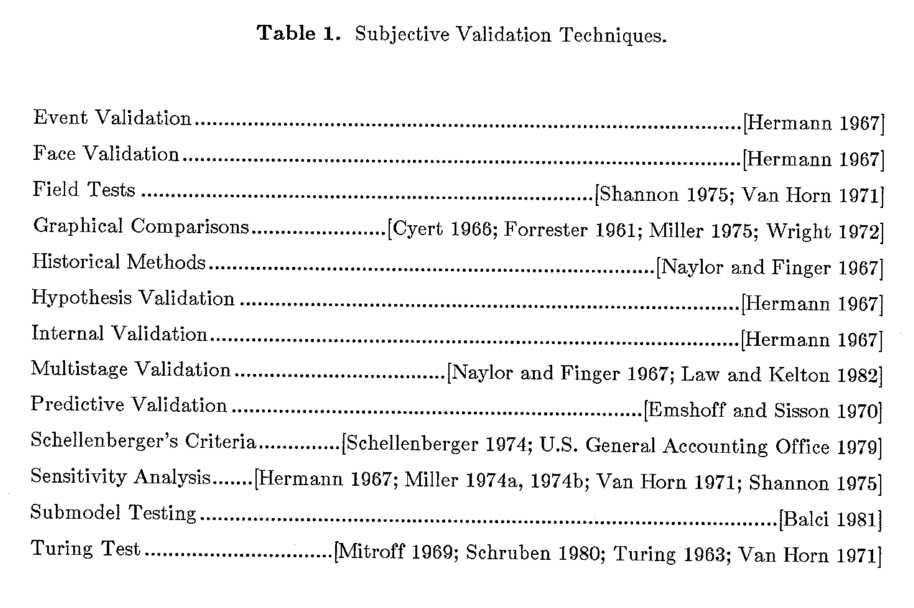
\includegraphics[width=.9\linewidth]{subjective_balci.png}
  \end{sidecaption}
\end{figure}

On se rend bien compte que dans le cadre des sciences humaines et sociales la possibilité de fixer par avance ce type de seuil n'a pas de sens, surtout dans un cadre explicatif.

%\textit{Que faut il entendre ici par partiellement ? Quels sont les leviers permettant au géographe de compenser cette perte de représentativité par un gain en compréhension sur le système à étudier ? }

Pour mieux comprendre quel est l'enjeu de cette délimitation entre un modèle réaliste et un modèle abstrait, il faut évoquer cette tension permanente qui nourrit les choix du modélisateur dans la construction d'un modèle explicatif. Deux attracteurs possibles et apparemment opposés, avec d'une part la volonté de se rattacher à une forme de réalisme au travers de l'injection d'une part maîtrisée de réalité tout au long du processus de construction\Anote{durand_observation}, et d'autre part une force qui nous pousse au contraire à se détacher de cette même empirie pour ne retenir que le matériel susceptible de servir l'objectif du modèle.

La sociologue et épistémologue \textcite{Bulle2005} a bien formalisé ce dilemne dans la nécessité pour tout modélisateur de positionner son modèle sur un gradient opposant le réalisme des causes des modèles explicatifs\Anote{bulle_modele_explicatif}, au réalisme des effets des modèles descriptifs.

Pour mieux comprendre quelles connaissances on peut attendre d'un tel positionnement sur ce gradient, le mieux est encore de commencer par évoquer un de ses extrêmes, en invoquant par exemple le modèle universellement connu de Schelling. De par sa portée d'application extrêmement générale et la nature très abstraite de ses paramètres, celui-ci constitue en soi un extrême intéressant pour comprendre où se situe encore l'explication lorsque le détachement de la réalité est à ce point exagéré. Sur ce point, les analyses de \textcite{Bulle2005} et \textcites{Phan2008, Phan2010} se réfèrent principalement à l'essai de \textcite{Sugden2002} pour évoquer quels types de relations entre les deux mondes on peut attendre de ce type de modèle épuré.

Les résultats qui dérivent de la mise en dynamique des règles dans le modèle de Schelling sont d'une telle universalité, d'une telle robustesse qu'il n'est plus question de confronter les résultats ainsi obtenus à la réalité. A cet égard, le potentiel explicatif de ce type de modèle s'oppose selon \textcite{Bulle2005} à tout réalisme empirique. De ce point de vue, \enquote{le modèle n'est pas tant une abstraction de la réalité qu’une réalité parallèle [...] bien que le monde du modèle soit plus simple que le monde réel, celui-ci n'est pas une simplification de l'autre. Le modèle est réaliste dans le même sens qu'un roman peut être appelé réaliste [...] les personnages et les lieux sont imaginaires, mais l'auteur doit nous convaincre qu'ils sont crédibles } \autocites[131]{Sugden2002}[10]{Phan2008}.

L'effet d'une telle recombinaison d'hypothèses revient à mettre en oeuvre un \enquote{monde crédible} où l'inférence inductive est mobilisée pour identifier des similitudes significatives entre les deux mondes. \autocites{Livet2006, Phan2008}. Tout le travail réside donc dans l'interprétation prudente qui peut être faite entre ces résultats d'un monde factice et d'une réalité.

Un processus commun utilisé dans toute oeuvre de fiction pour piquer la curiosité de l'observateur, la mise en exergue volontaire d'une tendance du monde réel dans un monde imaginaire permettant d'entamer une réflexion sur l'existence, la portée, la nature de cette même tendance dans le monde réel. Les villes ou les sociétés mises en avant dans des oeuvres de fiction de cinéma ou dans la littérature ne sont jamais que des mondes plus ou moins crédibles (Gotham City, 1984, Matrix, la série Black Mirror, etc.)  pour mettre en avant un discours, ou des tendances du monde réel sur lequel doit porter le questionnement. %(http://www.influxpress.com/imaginary-cities/ , \href{http://cybergeo.revues.org/1170#tocto1n9?}{cybergeo})

Si le discours scientifique n'a clairement pas cette obligation ludique, il n'en reste pas moins que ce processus de reconstruction crédible est déjà un outil formidable pour questionner les processus à l'oeuvre dans le monde réel\Anote{ruffat_samuel_ville}. Mais cette ambiguïté de lecture a déjà mené à de nombreux malentendus, d'une part envers le grand public \autocites{Forrester2007,Deffuant2003} qui pourrait prendre des résultats de simulation pour la réalité avec toutes les conséquences que cela suppose, mais également parfois entre scientifiques provenant de divers horizons. Ainsi après la lecture de la critique par \textcite{Chattoe2011} de l'article de \textcite{Yanoff2008}, il ressort toute la difficulté d'évaluer la méthodologie et le travail réalisé autour d'un modèle au travers d'une seule publication, notamment lorsque la fonction cognitive recherchée par les modélisateurs n'est pas décrite explicitement, ce qui provoque aussi ce décalage entre attente du lecteur et le processus réel de recherche qui sous-tend la construction du modèle (voir section \ref{sssec:equifinalite} pour plus de détails sur ce débat).

\textit{Doit-on se contenter de ce seul mode explicatif ? Existe-t-il un moyen pour renforcer la confiance dans la capacité explicative des hypothèses ainsi mobilisées ? }

\paragraph{Justifier des hypothèses par leurs qualités de représentation}
\label{justifier_hypothese}

%% DEBUT - EN ATTENTE DE LA REPONSE DE VARENNE %%
\textcite{Bulle2005} évoque bien l'existence de modèles à cheval entre potentialité explicative et potentialité descriptive. Ainsi \enquote{appliquée aux processus sociaux réels, la simulation peut allier au potentiel descriptif offert par l’imitation d’effets empiriquement observables, le potentiel explicatif que lui confère la mise en œuvre de relations causales effectives.}

A la différence de modèles trop simples qui n'offrent que de maigres accroches avec la réalité, c'est donc par la réintroduction maîtrisée de l'empirie dans les modèles de simulation construits que l'on pourrait espérer la mise en route progressive d'un processus de Validation en géographie ?

Un tel processus de justification paraît complexe, car celui-ci ne peut être conçu de façon homogène sans se heurter avec l'objectif même de toute modélisation qui, on le rappelle, n'est pas une construction guidée par la Validation mais une reconstruction mettant en oeuvre une simplification orientée par et pour un but. On ne parle pas d'un modèle comme d'un ensemble d'hypothèses de représentation homogène mais d'un ensemble d'hypothèses aux représentations hétérogènes.

Ce terme de \enquote{simplification} souvent employé reste d'emploi ambiguë, la modélisation nécessitant comme le dit \textcite{Haggett1965} non pas tant la mise en oeuvre d'une simplification aveugle, qu'une idéalisation guidée par la volonté de mettre à nu des propriétés du système observé. \textcite{Brunet2000}, pour qui la modélisation est également un processus de recherche, propose même pour éviter toute confusion sur les termes de dénuder la définition de modèle de cette fausse directivité, le modèle devenant dans sa version la plus épurée une \enquote{représentation formalisée d'un phénomène}; le terme \enquote{représentation} intégrant alors toute la complexité sous-jacente à une telle formalisation : \enquote{Il va de soi que cette représentation passe par plusieurs filtres, qui tous tendent des pièges : la perception du phénomène, sa représentation, la construction d'un modèle, l'interprétation du sens de ce modèle et la capacité du modèle à rendre compte du phénomène.}

Un point de vue semble-t-il partagé par Franck Varenne pour qui le terme simplification est \blockquote[{\cite{Varenne2008}}]{[...] un glissement d’attribution indu. Puisque l’usage du modèle est relatif (à un observateur et à un questionnement), on ne peut dire que le modèle doit être un objet simple en lui-même ou dans l’absolu. Il convient donc de regarder sous quel aspect exactement il doit apparaître simplificateur, sous quel aspect il devient un outil facilitateur, un outil de facilitation. [...] on comprend déjà qu’un modèle n’est pas ce qui est recherché en tant que tel, mais ce qui facilite la recherche d’information au sujet d’un système réel ou fictif, cela dans le cadre d’un processus à visée de représentation, de connaissance, de conceptualisation, de conception ou encore de transformation. Il est le moyen plus que la fin. C’est pourquoi je m’aventurerai, à partir de maintenant, à user plutôt du terme de facilitation que de celui de simplification [...]}.

Comme déjà évoqué par les géographes, ce n'est pas tant \enquote{le modèle} que ce qu'il y a \enquote{dans le modèle} qui nous intéresse \autocites{Sanders2000, Besse2000}.

Seulement comment analyser la pertinence d'une représentation prise en dehors de son contexte ? Les choix intervenant lors d'une modélisation ne répondent pas à une logique universelle pré-établie, et sont motivés et modulés par un ou plusieurs objectif(s) qui n’interviennent pas forcément de façon volontaire pour guider la modélisation. \textcite{Varenne2013b} ayant par ailleurs identifié une vingtaine de ces \enquote{fonctions de facilité de médiation} pouvant très bien se cumuler lorsqu’on observe un modèle. Or, il me semble qu'une fois rapporté à la structure interne du modèle de simulation, on est bien obligé de constater l'impact que peut avoir cette diversité d'objectifs dans la mobilisation d’une ou plusieurs représentations, dont certaines peuvent être concurrentes, pour une même hypothèse dans le modèle. Est-ce pour dénoter une entité réelle (un agent = un individu, une ville, une innovation ) ? Est-ce dans le but de simplifier pour la compréhension ? pour les performances ? pour répondre au principe de parcimonie ? Ou tout à la fois ? (une population d'agents homogènes devenant une équation de croissance par exemple ). Était-ce un choix fait à la suite d’une multitude d'autre essais (différentes équations plus ou moins représentatives du phénomène à considérer) ? etc. Dans le cas d'un modèle de migration inter-ville, il est en effet plus intéressant de mobiliser les populations de façon agrégée si l'on s'intéresse aux règles intervenant dans la dynamique d'interactions entre les villes, par contre, s'il s'agit d'observer l'impact que peuvent avoir des règles de comportements sur ces interactions, ce niveau peut devenir pertinent; cette approche ne chassant évidemment pas la première, au contraire les couplages étant bienvenus. En définitive, il n'y a aucune raison pour que les hypothèses intégrées aux modèles de simulation soit homogènes. Ainsi, pour Franck Varenne, pour identifier \textit{a posteriori} quelles sont les fonctions épistémiques mobilisées, et donc par extension déterminer dans quelle mesure l'intérêt porté à la validation a pu être très diffèrent lors de la construction du modèle (pour un modèle de simulation pédagogique, la validation n’est par exemple clairement pas une priorité ...), il est nécessaire de se poser la question pour chacune des hypothèses représentées dans le modèle de simulation : est-ce une dénotation ? une exemplification (métaphore) ? La qualité de représentation se détermine au cas par cas, en fonction des objectifs et des choix de modélisation associés à chaque hypothèse. Il s'agit ici de déterminer l'\enquote{engagement ontologique} des simulations.

Normalement tous ces choix devraient être explicités, ce qui est rarement le cas, vu la complexité d'une tâche qui appelle pour être sérieuse l'analyse d'une activité de raisonnement accompagnant le modèle dont les jalons ont bien souvent disparu.

La tendance à la pluriformalisation\Anote{pluriformaliser} permise par les modèles multi-agents ne vient pas non plus faciliter cette tâche, car ces modèles de simulation qui peuvent déjà intégrer -et c'est d'ailleurs pour cela qu'ils ont autant de succès- sans problème une hétérogénéité d'échelles, de niveaux d'abstraction, de modèles, doivent aussi compter avec l'intégration de formalismes mobilisant des temporalités et/ou des échelles différentes \autocites{Varenne2008,Varenne2012a}. Ces couplages n'étant pas toujours évidents, y compris au niveau informatique où des artefacts (c'est-à-dire l'apparition de mécanismes nécessaires à l'implémentation\Anote{exemple_slocal} mais non prévus et difficiles à expliquer d'un point de vue purement théorique) peuvent rapidement venir perturber les ontologies réalisées en amont.

Même les modélisateurs ont parfois du mal à s'y retrouver, par exemple il n'est pas toujours évident d'expliquer pourquoi on a choisi de coupler pour certains mécanismes le formalisme agents avec celui des équations différentielles ? Il faut alors comprendre que dans certains cas, c'est aussi ce qui a pu motiver le modèle, l'intérêt de la pluriformalisation étant justement ce qu'il faut démontrer en comparaison des approches traditionnelles prisent séparément. Plusieurs réflexions ont montré qu'il s'agissait d'un type de modélisation en devenir et en voie de démocratisation, les formalismes pour la simulation informatique (multi-agents, micro-simulation, automates cellulaires) ou mathématique (systèmes dynamiques) utilisés n'ayant jamais eu vocation à s'opposer (approche individu centrée contre approche mathématique traditionnelle) comme on aimerait parfois nous le faire croire \autocites{Sanders2013, Banos2013}.

Varenne s’intéresse de beaucoup plus près aux effets de cette hétérogénéité interne aux simulations d’un point de vue épistémologique, et ce sont d'ailleurs ses articles sur cette question \autocite{Varenne2013b,Varenne2013c} et plusieurs échanges privés (daté de 2014/2015) avec lui qui ont inspiré certaines de ces dernières réflexions. Il nous sera toutefois difficile d’aller au-delà sur cette analyse de la \enquote{représentativité des hypothèses fonction des objectifs}, car même si celle-ci est une question passionnante, elle reste un axe de recherche avant tout théorique et en plein développement. Aucun n'exemple concret ne permet pour le moment d'illustrer la forme que pourrait prendre une telle analyse.

Un autre argument vient condamner encore plus fermement l'idée de justifier d'une Validation des modèles basée sur la qualité de représentation de ses hypothèses. Celui-ci a déjà été effleuré en traitant de philosophie des sciences dans la section \ref{sssec:philo_sciences}. Le processus de validation se heurte rapidement à la différence de nature entre les résultats produits par des hypothèses \textit{reconstruites} et le monde réel\Anote{bulle_modele_autonome}. Tout comme le substrat est artificiel, le résultat produit par cette dynamique reste le produit d'un monde reconstruit - \textit{in silico} - L'existence de ce nouveau niveau d'empirie amène les épistémologues comme Franck Varenne à parler ici d'\enquote{expériences concrètes du second genre} faisant alors de la simulation une \enquote{quasi-expérimentation} \autocites{Varenne2001, Varenne2007, Phan2008, Phan2010}

On en déduit que quel que soit notre placement sur ce gradient, il est effectivement vain de chercher à valider un modèle en usant d'un quelconque \enquote{seuil de suffisance} caractérisant \enquote{l'injection de réalisme à atteindre qui autoriserait une inférence certaine sur le monde réel}, puisque de toute façon cette inférence s'appuie sur un résultat \enquote{artificiel} forcément discutable\Anote{phan_livet_modele}.

\paragraph{Inverser le problème de la Validation pour désengager cet objectif de correspondance au réel}
\label{p:inverser_problematique}

Une autre façon donc de dépasser cette problématique de la Validation est d'accepter le fait que le réalisme des hypothèses ne soit plus vraiment un objectif, mais plutôt la réalisation conséquente d'une expertise qui tient essentiellement de l'angle théorique choisi pour éclairer un problème.

Autrement dit, la confiance établie dans les capacités explicatives des hypothèses choisies ne se juge pas tant dans la comparaison des résultats attendus avec le réel observé, que dans l'exploration du monde crédible ainsi simulé en fonction de critères experts construits sur une observation du réel, dans l'espoir d'en dégager une connaissance qui doit encore être vérifiée\Anote{denise_geopoint}.

Le problème est ici en quelque sorte inversé, ce n'est plus une qualification directe du réel qui est visée par le modèle, mais le modèle qui est visé par notre compréhension du réel au travers de critères experts. Ceux-ci viennent questionner et mettre en tension ce monde virtuel en lui imposant de nouvelles contraintes, révélant par là même les forces et les faiblesses de nos hypothèses dans le modèle. On oppose dans la construction du modèle \enquote{un jeu d'hypothèses susceptible de produire des résultats attendus}, à la réalité des conclusions apportées par la \enquote{mise en oeuvre effective d'une dynamique}.

Cette situation semble ramener le problème de la \enquote{Validation} à une évaluation \enquote{terme à terme} entre hypothèses et critères experts (les faits stylisés par exemple) susceptible d'en rendre compte. Pour \textcite{Bulle2005}, il sera donc toujours nécessaire et légitime de questionner la pertinence des rapports mesurés entre les liens causaux proposés dans le modèle et le ou les critères qui sont censés en rendre compte.

C’est me semble-t-il ce que voulait dire Frédéric Amblard \textcite{Amblard2006} lorsqu’il parlait du rapport liant la détection de comportements de la \enquote{validation interne} à leur utilisation comme support d’une partie de la \enquote{validation externe}.

\blockquote[\cite{Amblard2006}]{L'analyse de sensibilité, si elle peut s'appliquer pour tester la robustesse des résultats d'un modèle, peut également être utilisée pour tester la robustesse de la structure du modèle. En modifiant les hypothèses réalisées dans le modèle, par exemple en modifiant les structures organisationnelles, le modélisateur obtient des indices relatifs à la stabilité de son modèle et de ses hypothèses. Ces indices lui permettent précisément de jauger l'importance du choix d’une hypothèse et l’influence de son remplacement par une autre sur un aspect particulier du modèle. [...] Une autre propriété importante qu'il s'agit d'étudier au cours de cette étape de validation interne, concerne les classes de comportements produites par le modèle. Les simulations multi-agents produisent ce qui est assez communément appelé des \enquote{comportements émergents}  (voir chapitres 14, 16 et 17), c'est-à-dire des comportements qui ne sont pas exprimables en utilisant uniquement les hypothèses réalisées sur les comportements individuels}.

Deux propriétés qui font ainsi écho à une méthode de la validation externe qui \enquote{[...] consiste à rapprocher les classes de comportements (identifiées lors de la validation interne) à des comportements saillants du système-cible : les faits stylisés.}

\blockquote[\cite{Amblard2006}]{Ce rapprochement, s’il peut être fait avec des faits stylisés identifiés a posteriori (permettant par exemple de découvrir dans les phénomènes empiriques, des comportements stylisés qui auraient pu passer inaperçus), possède, on le sent bien, plus de force lorsque les faits stylisés sont déterminés avant même la modélisation comme des comportements que l'on cherche à reproduire par le modèle ou dont on se servira comme un critère de validation parmi d'autres (rétrodiction).}

Ce point nous incite à pratiquer une évaluation à contre-pied de la démarche habituelle, alternant validation interne, puis externe. Le modélisateur se saisit un moment de cette légitimité évoquée par \textcite{Bulle2005} en devenant celui qui dirige la mise en tension de cette relation. On met alors de côté un instant la validation interne comme exploration non dirigée des comportements du modèle pour se concentrer sur une exploration, certes moins complète mais plus dirigiste et plus précise, où c'est la capacité du modèle de simulation à opérer ce rapprochement qui permet d'accompagner le raisonnement. Les modélisateurs peuvent alors introduire les hypothèses dans le modèle de simulation dans le but de satisfaire, ou \textbf{de ne pas satisfaire} ces critères.

En effet, on a bien précisé par exemple que l'objectif de correspondance avec les données n'était plus un critère prioritaire dans l'établissement de tels modèles de compréhension, sinon pourquoi ne pas se contenter d'un simple modèle de Gibrat pour expliquer la hiérarchisation des systèmes de villes ?

%Cette inversion soulève de nombreuses remarques que l'on va tenter d'articuler par la suite.
Cette inversion soulève plusieurs remarques. On se rend compte que les critères d'évaluation deviennent dans un tel processus aussi importants que les hypothèses dont ils sont censés rendre compte. L'introduction de chaque nouveau critère met un peu plus en tension la dynamique produite par le jeu d'hypothèses proposé par le modélisateur, et rend donc un peu plus difficile ce rapprochement. Autrement dit, le modélisateur pose les questions par les critères qu'il mobilise, et le modèle de simulation tente ce rapprochement avec les hypothèses et les contraintes de paramètres qu'on lui a fourni. C'est une tentative de calibrage dont on minore la capacité à calibrer (ce n'est pas forcément ce qui nous intéresse en premier lieu), et dont on majore la capacité à stresser la structure du modèle.

Cette solution a l'avantage d'empêcher la construction de modèles de simulation exprimant seulement un comportement \enquote{vraisemblable} vis-à-vis des critères souvent subjectifs que l'on se fixe en premier lieu lorsqu'on construit un modèle (on parle de \textit{face validity}). Il est problématique à mon sens de construire un raisonnement en se basant sur des interprétations dont on ne maîtrise pas la fiabilité. Autrement dit, le \enquote{vraisemblable} n'est plus suffisant pour assurer un raisonnement, et il est nécessaire pour la construction des modèles de se doter d'un protocole d'évaluation plus systématique.

Il faut détailler à présent les modalités qui sous-tendent cette nouvelle façon de construire de la connaissance.

\paragraph{L'abduction un phénomène clef dans l'activité de modélisation}
\label{p:abduction}


La présence d'une hypothèse dans le modèle se justifie donc autant par l'expertise du modélisateur que par son adéquation, ou sa non-adéquation \textbf{potentielle} avec différents critères de validation. La subjectivité de l'expérimentateur joue sur les deux tableaux, et donne à voir dans cette subtile inter-dépendance qui relie le choix des hypothèses et le choix des critères une forme d'incertitude quant au résultat assez difficile à prévoir et quantifier.

Que se passe-t-il en effet lorsque le potentiel explicatif d'une hypothèse pourtant appuyé par des résultats empiriques constatés dans le système observé s'avère invalidée par une analyse de sensibilité ou un critère d'évaluation ? Et cela, alors même que l'expérimentateur considère celle-ci comme étant indispensable au développement d'une dynamique donnée ? Que se passe-t-il au contraire lorsqu'un critère d'évaluation est atteint alors que cela n'était pas attendu au vu de la structure actuelle du modèle ?

%La fonction heuristique de la simulation pouvant s'exprimer tout autant dans cette \enquote{surprise} d'une divergence entre le potentiel investit dans les hypothèses et les critères selectionnés, que dans la surprise suivant l'introduction de nouveaux critères contraignant le modèle, et remettant en cause ce même potentiel de représentation investit dans certaines hypothèses.

Il y a une divergence nécessaire entre la volonté du modélisateur de rendre compte d'un système observé par un réseau d'hypothèses qui lui paraît parcimonieux, nécessaire et cohérent d'un point de vue thématique (le potentiel investi), et la réponse effective apportée par la mise en dynamique de ces causalités lues au travers des critères selectionnés pour en rendre compte. % la possibilité d'infirmer ou d'affirmer de nouvelle connaissances, avec le développement de nouveaux critères, de nouvelles hypothèses ayant jusque là échappé aux raisonnement du modélisateur.

\foreignblockquote{english}[{\cite[219]{Hermann1967}}]{In developing a game or simulation, the designer is required to be explicit about the nature and relationships between the units in the operating system and their counterparts in the observable universe. He must specify the conditions which cause a relationship to vary. In constructing an operating model a connection between previously unrelated findings may be discovered. Alternatively, a specific gap in knowledge my be pinpointed and hypotheses required by the model my be advanced to provide an explanation.}

\foreignblockquote{english}[{\cite[226]{Hermann1967}}]{In all probability some distributions of events or some kinds of hypotheses will produce results with unacceptable divergence between the operating model and the observable universe. Although these incongruous may not pinpoint the inadequacy in the model, they should provide a diagnosis of the general area which seems unrepresentative.} 

La surprise volontaire ou involontairement produite au cours de cette divergence, et qui accompagne généralement l'activité de modélisation, revient sous le nom d'abduction, le terme venant de Charles S. Peirce \autocites{Besse2000, Banos2013, Phan2006, Livet2014}.

On a déjà précisé en s'appuyant sur les propos de Ian Hacking \autocites{Hacking1989,Hacking2003, Hacking2006} que ce phénomène d'abduction n'était pas un héritage du seul cadre logique, mais une propriété inhérente à l'humain \Anote{stanislas}, existante de façon préalable à ses créateurs Aristote, ou Peirce.
%Cette logique bayésienne qui consiste à formuler une hypothèse a priori de façon consciente ou inconsciente \Anote{kauffman}, prise de façon rapide ou lente, basé sur nos connaissances passés ou sur notre environnement présent, pour la confronter et la réévaluer au yeux de la réalité de façon itérative correspond assez bien il me semble à ce que l'on pourrait apeller \enquote{abduction}, apellée également \enquote{inférence de la meilleure explication}.

Dans l'utilisation des modèles de simulation d'une part, ce n'est pas le monde réel qui nous surprend, mais ce qui se passe dans le modèle de simulation, et d'autre part il est plus intéressant d'adopter une démarche active et créative dans la mobilisation des hypothèses, afin de maximiser la surprise plutôt que de la miminiser, de dépasser son horizon de connaissance plutôt que de s'y conforter. Comme le résume bien \textcite{Banos2013} dans son HDR, \enquote{l’esprit même de l’abduction au sens de Peirce, désignant cette capacité de l’être humain à générer des hypothèses temporaires à partir de l’information incomplète dont il dispose. Appliquée à la démarche scientifique, l’abduction renvoie ainsi à la capacité du scientifique à se mettre en position d’étonnement, à se laisser guider par la recherche de l’inattendu et plus généralement à laisser libre cours à sa créativité.}

Comme on pouvait alors s'y attendre, les motifs développés par les modélisateurs soutenant cette approche sont très loin de ceux attendus pour la prédiction, ou c'est d'abord la robustesse des résultats qui prime, car \enquote{[...] dans le cas d’une modélisation compréhensive, où l’objectif est d’apprendre des propriétés du système que l’on reconstruit \textit{in silico}, le fait d’avoir, pour une partie des conditions expérimentales des comportements très erratiques du système, loin de discréditer le modèle nous apprend au contraire des éléments de son fonctionnement et nous permet même d’anticiper le fonctionnement du phénomène modélisé. Si sous certaines conditions le modèle est très instable c’est une information très enrichissante sur le modèle et sur le phénomène considéré.} \autocite{Amblard2010}.

Force aussi de constater que cette incrémentalité dans la construction d'un modèle de simulation ne suit pas vraiment un modèle linéaire de développement, et s'accompagne, au moins dans les sciences humaines et sociales d'une activité de raisonnement en partie imprévisible. Ainsi, il peut paraître paradoxal pour un modélisateur débutant de voir à quel point il est important de \enquote{malmener} les modèles que l'on a précédemment construits avec raison et parcimonie. L'important ici nous dit \textcite{Amblard2010}, c'est que cela participe à l'élaboration de la compréhension ou de l'explication des phénomènes considérés. Car, comme le dit \textcite[65]{Banos2013} dans son tout premier principe, modéliser c'est avant tout apprendre.

D'autres définitions de l'abduction \Anote{abduction_definitions} permettent de mettre en valeur d'autres de ces propriétés, la création en est une, mais avec celle-ci vient aussi la sélection. Si l'on se rapporte aux processus de cognition, la conscience apparaitrait par exemple comme un filtre discrétisant, sélectif, d'une pensée inconsciente fluctuante et résolument continue. On peut supposer que lors de la modélisation, ce type de processus est également à l'oeuvre, et il n'est pas rare lorsqu'on construit un modèle de simulation d'avoir à choisir, ou à ne pas choisir, avec plusieurs hypothèses ou implémentations d'hypothèses alternatives. Le deuxième choix expliquant aussi en partie pourquoi les interfaces utilisateurs de nombreux modèles de simulation Netlogo sont aussi riches en boutons de sélection...


%Cela soulève la possibilité d'hypothèse explicative concurrente ou inter-dépendante dans l'apparition d'un phénomène, dont certaine échappe forcément au seul modélisateur géographe du fait par exemple de la nature inter-disciplinaire des objets engagés, auquel il faut encore appliquer une selection plus consciente en décidant de mettre plus ou moins en avant des hypothèses susceptible de surprise.

%La surprise ne vient donc pas seulement du modèle, mais aussi de ce que font les autres manipulant les modèles, surtout dans le contexte inter-disciplinaire ou nous évoluons, les limites de nos connaissances se manifestant assez vite lorsqu'il s'agit d'étudier un phénomène ou un objet partagé, comme les villes par exemple.


\paragraph{Quels critères d'évaluation pour quelles mesures des hypothèses ?}
\label{p:critere_evaluation}



% S'exprime dans une dynamique ?
Il y a plusieurs problèmes qui limitent cette possibilité d'une comparaison directe avec les données. Au tout début de notre argumentaire, on a vu avec Hermann que la mobilisation d'un seul critère quantitatif ne pouvait pas suffire à garantir une quelconque explication. Avec suffisament de degrés de liberté, que cela soit par le nombre d'hypothèses mobilisées, ou le nombre de paramètres que l'on met à disposition d'un optimiseur humain ou ordinateur, on trouvera toujours un moyen de se rapprocher des données. \textcite[17]{Amblard2006} parle, par exemple, de surdétermination des paramètres aux données.

%Problème de nature des données, et de leur disponibilités
Un autre problème se pose également avec la mobilisation des données. Du fait de l'\textit{Observational Dilemna}, cette solution d'une comparaison terme à terme explicite entre hypothèses constituantes du modèle et critères n'apparait pas faisable selon \textcite{Batty2001} : \foreignquote{english}{In principle, each element of this process should be explicit and should be capable of being validated with observed data. In practice, this is rarely if ever the case. The data set would be too large, it would be impossible to collect in its entirety, it may be impossible to even observe and measure. Yet the processes are known to be important. Other criteria must thus be used.}

On peut ajouter à cela une autre limite concernant les données, on a en effet vu que toutes les hypothèses d'un modèle n'avaient aucune raison de se placer au même niveau d'abstraction, ou d'appartenir au même formalisme. Il est par exemple déjà difficile d'accéder à des données dans une fenêtre spatio-temporelle donnée, est-il possible d'en avoir sur plusieurs fenêtres, voire plusieurs fenêtres simultanées ?

Le dilemne commence à apparaître clairement, car il ne s'agit pas de tomber dans une \foreignquote{english}{Forrester Strategy}, en abandonnant toute volonté de justifier la chaîne d'hypothèses mobilisées dans les modèles.

% multiplication des critères ?
On peut de nouveau faire appel à l'analyse d'Hermann, dont l'originalité réside aussi dans les remarques très justes et très précoces qu'il a formulées sur la relativité des hypothèses \textbf{mais aussi des critères mobilisés} dans les modèles. Celui-ci est tout à fait conscient qu'il ne s'agit pour l'une comme pour l'autre que d'assertions sur la réalité. Il propose donc d'essayer de faire au mieux. En adoptant une validation multi-critère\Anote{methode_hermann} intégrant les objectifs ayant guidé la construction du modèle, il espère ainsi renforcer le crédit qu'il est possible d'apporter aux simulations\Anote{conclusion_hermann}, tout en restant sceptique\Anote{hermann_doute} sur la possibilité d'inférer en retour sur les systèmes observés.

\foreignblockquote{english}[\cite{Hermann1967}]{We have arrived at the position, then, that multiple validity criteria are needed because of the error of measurement and because of the recognition that criteria can be only assertions about \enquote{reality}}

Pour \textcite{Amblard2006}, si cette validation externe basée sur une comparaison quantitative avec les données n'est pas impossible, elle n'en reste pas moins difficile à mettre en oeuvre de façon systématique, en partie pour les raisons évoquées ci-dessus. L'appel à des critères d'évaluation plus qualitatifs (\enquote{faits stylisés}) reste le plus évident à mettre en oeuvre. Un point de vue partagé par \textcite{Batty2001}, pour qui \foreignquote{english}{ [...] complex systems models have multiple causes which display a heterogeneity of processes that are impossible to observe in their entirety. The focus is on more qualitative evaluation of a model’s plausibility in ways that relate to prior analysis of the model’s structure.}

Cette démultiplication des critères d'évaluation, même si c'est une opération qui reste indispensable, ne nous sauvera pas d'un autre problème. Il n'y a pas de seuil de suffisance à chercher dans la représentativité des hypothèses, mais également dans leur mise en cohérence/relation, puisque celle-ci tient là encore d'une reconstruction guidée par une but. La recherche d'une cohérence interne au modèle n'apporte pas plus de garantie sur la transférabilité des hypothèses à la réalité. Ce qui ne veut pas dire qu'il ne doit pas y en avoir, seulement celles-ci doivent être faites pour les bonnes raisons, et non pas pour se donner l'illusion d'une meilleure inférence des conclusions du modèle au système observé.

\foreignblockquote{english}[\cite{OSullivan2004}]{There is a many to one relationship between the structure of models and the behaviour they produce, so that many models can account for the same observed outcome. This is the equifinality problem. One common (incorrect) response to the problem is to examine the internal consistency of the model, and to assume that internal consistency guarantees a true representation of reality. Alternatively, we resort to calibration, and adjust model parameters until a best fit to historical data is achieved. Calibration is a complex technical procedure, but ultimately offers no escape. At best, observational data can be replicated more or less closely, but this provides no guarantee as to a model’s accuracy as a representation, nor does it exclude any other model, or another choice of parameters.}

Outre donc la question de la disponibilité des données en sciences humaines et sociales, l'\textit{Observational Dilemna} sous-tend également l'impossibilité d'établir l'unicité des hypothèses avancées pour décrire un phénomène, mais aussi par extension celle des critères d'évaluation, qui restent eux aussi des construits formulés sur la base d'une observation du système observé. Capturer toute la substance d'un phénomène émergent dans un ou plusieurs critères d'évaluation reste difficile, voire impossible.

Cette variabilité exprimée dans la construction et la paramétrisation des structures causales et des critères associés renvoie à ce phénomène bien connu des modélisateurs en sciences humaines et sociales, à savoir l'équifinalité (voir la figure \ref{fig:S_equifinalite}).

\begin{figure}[htbp]
\begin{sidecaption}[Schéma de représentation de l'équifinalité]{Schéma de représentation de l'équifinalité, inspiré de \autocite{Richardson2002} : \foreignquote{english}{Illustration showing that not only can a particular system state (outcome) can be reached via different trajectories from the same starting conditions, but also that different starting conditions may also lead to the same system state. Of course, the reverse case is also a possibility in that different starting conditions may lead to different outcomes and multiple runs from the same starting conditions may also result in different outcomes.}}[fig:S_equifinalite]
  \centering
 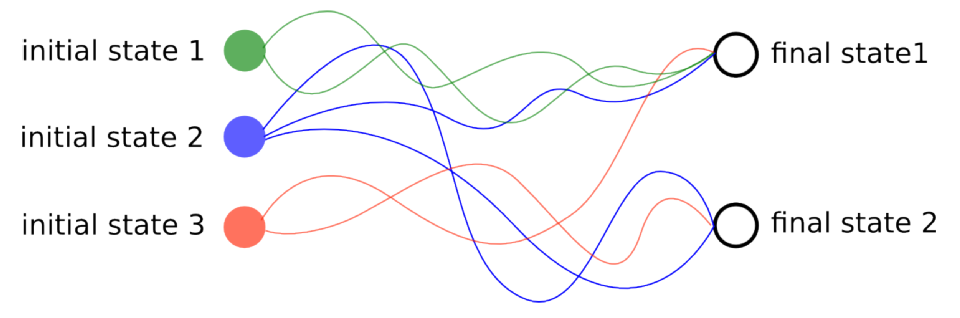
\includegraphics[width=.9\linewidth]{equifinalite.png}
  \end{sidecaption}
\end{figure}

L'équifinalité est un concept provenant à l'origine d'un phénomène observé en embryologie \Anote{embryon}, généralisé ensuite par Bertalanffy comme \textbf{une propriété fondamentale des systèmes ouverts} (voir la section \ref{subsec:gst} en annexe pour une remise en contexte du terme). Celui-ci reste un terme couramment employé dans la littérature, et que l'on retrouve associé à une limitation dans la \enquote{Vérification} \Anote{verification_philo} en philosophie :

\foreignblockquote{english}[\cites{OSullivan2004,Oreskes1994}]{\textcite{Oreskes1994} crisply describe the problem: it is impossible to verify the representational truth of any model of an open system. There is a many to one relationship between the structure of models and the behaviour they produce, so that many models can account for the same observed outcome. This is the equifinality problem.}


Cette variabilité est à la fois conséquence naturelle du processus de raisonnement, mais également une conséquence logique liée à la nature insaisissable du réel. Toutefois, là où on pourrait voir cet effet comme positif et cumulatif, l'équifinalité est souvent présentée comme un défaut de l'outil et de la discipline. La section suivante essaye de voir les solutions proposées par la communauté des modélisateurs dans la mise en perspective d'un débat récent. Une autre proposition, plus proche de nos pratiques sera ensuite présentée, mais nécessitera de repenser la façon dont sont construits et valorisés les modèles de simulation. % dans un cadre d'analyse qui s'appuie sur l'existant pour mettre en valeur les aspects dynamique, cumulatif, et local de cette activité.

\subsubsection{Repenser la question de l'équifinalité}
\label{sssec:equifinalite}

Pour résumer, on a vu dès le départ avec \textcite{Hermann1967}, que la Validation était indissociable d'un contexte, et que celle-ci posait de fait la question de la représentativité des hypothèses vis-à-vis des critères mobilisés.

En cherchant comment on pouvait mesurer la qualité explicative des modèles réalisés, on s'est aperçu que la recherche d'un seuil de réalisme adéquat n'était pas un bon argument pour guider l'intégration des hypothèses sur les entités ou les activités à injecter dans nos modèles. En développant jusqu'au bout l'argument d'une justification possible dans le choix fait des modélisateurs sur la représentativité des hypothèses, on s'est rendu compte d'une part que c'était difficile du fait de l'hétérogénéité et de la multidimensionnalité de celles-ci, et d'autre part qu'il s'agissait pour le moment plus d'une question épistémologique a posteriori que d'un comportement assumé par les modélisateurs. Peu de modélisateurs font aujourd'hui cet effort d'explicitation des fonctions facilitantes associées à chacune des hypothèses en les rapportant au raisonnement accompagnant la construction du modèle.

Comme il n'est pas non plus possible de garantir une validation empirique terme à terme entre hypothèses et données, il est nécessaire d'accumuler différents critères quantitatifs et qualitatifs non pas pour se rapprocher d'un fonctionnement du réel, mais plutôt là aussi pour garantir la cohérence d'une \enquote{reconstruction d'un jeu de causalité identifié comme pertinent dans la reproduction d'un phénomène} que l'on veut confronter \enquote{aux mesures censées rendre compte de ce phénomène dans la réalité}. Le jeu abductif vient ici encourager ou perturber ce rapprochement entre hypothèses sélectionnées et critères mobilisés.

Il a été également avancé qu'une partie des connaissances dégagées durant ce jeu abductif rythmant la construction des modèles était liée au fait que le modèle de simulation servait de laboratoire non pas pour modéliser et confronter le monde réel, mais plutôt pour modéliser et confronter nos \textit{a priori} théoriques sur le fonctionnement du monde observé. A ce titre, les échecs induisent un retour sur la théorie aussi stimulant que les réussites, ce qui motive ainsi la prise de risque et la créativité dans les hypothèses ou les critères avancés.

Chacun de ces arguments renvoie normalement l'image d'une activité de Validation indissociable d'un contexte donné. Pour reprendre les mots de \textcite{Amblard2006} \enquote{[...] les questions pour la validation des modèles ne devraient jamais être abordées en dehors des questions relatives à leurs usages.}

L'équifinalité vient ici compliquer ce constat, car elle fournit l'image inverse si l'on n'y prend gare, en facilitant l'idée qu'une construction peut être facilement remplacée par une autre, sans que la question du contexte ne soit abordée. Le problème n'est pas que cela puisse être vrai ou faux, car comme on va le voir ensuite, la possibilité de rendre compte différemment d'un même phénomène a été intégré depuis longtemps dans les différentes modélisations supportées en géographie, mais plutôt que des personnes extérieures à une communauté puissent penser que c'est un défaut des techniques ou des méthodologies utilisées, alors que c'est un défaut propre à l'étude des systèmes complexes, et donc également des systèmes sociaux \autocite{Elsenbroich2012}. Il est également dommageable de voir apparaitre des discours pointant comme contradictoires des modèles ou des résultats de modèles étudiant le même phénomène dans des disciplines diverses, alors même qu'on pourrait y voir au contraire une complémentarité.

Une entrée par les critiques récentes formulées sur ce cadre d'analyse historique des \enquote{Sciences Génératives} formulées par Epstein peut être un bon exemple pour montrer que l'équifinalité, si l'on ne la justifie pas, peut grever la crédibilité des modèles présentés. Elle peut même, comme on va le décrire dans la section suivante, fournir le support biaisé à un argumentaire qui décrédibilise l'apport explicatif permis par l'utilisation de cet outil simulation en sciences humaines et sociales. Un groupe de sociologues proposent de répondre à ces critiques par un nouveau cadre d'analyse.

%Débat CONTE / EPSTEIN, résoudre equifinalite en justifiant d'une causalite
\paragraph{Faire appel à un nouveau cadre d'analyse ?}
\label{p:cadre_analyse}


%L'etude de cette problématique de l'équifinalité à l'orée des débats ayant lieu dans une communauté inter-disciplinaire telle que celle gravitant autour du journal JASSS est intéressante car elle introduit chez les sociologues un cadre pour penser la construction et l'évaluation des modèles, d'origines assez ancienne, qui intègre certains des éléments discutés précédemment : \enquote{les mécanismes générateurs}.

La critique de la simulation due à l’équifinalité par \textcite{Yanoff2008}  s’appuie ainsi sur le modèle des Anasazi \autocites{Dean2000, Axtell2002} pour proposer une critique générale des \textit{Artificial Societies} \Anote{desuet_as}.

\blockquote[{\cite[326-327]{Schmitt2014}}]{\textit{The Artificial Anasazi Project} a pour but de comprendre la trajectoire démographique des Anasazis, une société amérindienne ayant vécu dans la Long House Valley, au sud- ouest des États-Unis, durant la préhistoire (200 – 1400 ap. J.C.). Ce projet utilise un modèle multi-agents pour simuler le développement d’une société artificielle constituée de ménages amérindiens dans un environnement évolutif, caractéristique de la zone et de l’époque. Les sorties de ces simulations sont ensuite comparées à des bases de données empiriques archéologiques et paléo-environnementales.[...] Il existe deux grands types de dynamiques dans le modèle : celles de l’environnement et celles des agents. Les dynamiques de l’environnement sont simulées grâce aux inputs des données environnementales à chaque itération (représentant une année) de la simulation [...] Les agents représentent des ménages caractérisés par leur âge (à partir du moment de leur formation), leur taille (en nombre de personnes), leur consommation annuelle en maïs, leur capacité de réserve de maïs, leur localisation, et des indicateurs liés aux possibilités de mariage des femmes du ménage. Les règles d’interactions entre agents et avec l’environnement explicitent le comportement de choix de localisation de l’habitat et des champs cultivés par les agents. Une itération représente une année durant laquelle les agents cultivent leur parcelle. À la fin de cette période, les agents peuvent décider ou non de relocaliser soit leur habitat, soit leur parcelle de culture ou les deux, en fonction de leur capacité à couvrir leurs besoins nutritionnels cette année-là. La localisation simulée des habitats et des cultures est cartographiée année après année et comparée aux données.}

Ce modèle et sa dynamique ont été tant de fois répliqués, analysés et cartographiés que leurs défauts sont bien connus des modélisateurs. Malgré cela, ce modèle possède toujours une aura et une symbolique très forte, car il a ouvert la voie à d'autres modèles de simulation en archéologie, et en sciences sociales \autocites{Janssen2009, Stonedahl2010, Schmitt2013}[151]{Schmitt2014}.
Le \enquote{motto} bien connu d'Epstein pour une \textit{generative social science} \foreignquote{english}{If you didn't grow it, you didn't explain its emergence} \autocites{Epstein1996} reste aussi une source d'inspiration pour de très nombreux modélisateurs, malgré les critiques. Grüne-Yanoff n'ignore probablement pas que lorsqu'il s'attaque à ce modèle assez symbolique, il s'attaque aux pratiques de toute une communauté dont il ne fait \textit{a priori} pas partie. Une remarque de \textcite{Chattoe2011} qui peut paraître clanique au premier abord, et dont il faut aussi nuancer la portée, car on peut aussi voir dans cette critique la possibilité pour les modélisateurs d'améliorer les formes prises par cette communication autour des modèles, et des méthodologies associées. \textcite{Elsenbroich2012} résume le problème ainsi :

\foreignblockquote{english}[\cite{Elsenbroich2012}]{Grüne-Yanoff argues that this simulation does not give a causal explanation of the population dynamics of the Anazasi. The argument is not that the simulation is not an explanation of the Anazasi population but that it is not a causal explanation. The simulation does not tell a full causal history of the population dynamics, for example, the total exodus is not an outcome of any run of the simulation, thus leaving the explanation partial. Grüne-Yanoff argues that there is no such thing as a partial causal explanation. A causal explanation has to give a full account of all interactions leading to a phenomenon as there is no formal criterion to distinguish bad partial causal explanations from good partial causal explanations.}

Ce problème fondamental que tacle Grüne-Yanoff sans vraiment le nommer dans son texte, c'est l'équifinalité, et plus précisément l'équifinalité telle qu'on peut la comprendre dans ce cadre d'analyse qu'est la science générative définie par Epstein. Effectivement, même \textcite{Chattoe2011} qui critique de façon très virulente les propos de \textcite{Yanoff2008} doit bien admettre, avec d'autres, que l'existence d'un critère unique - qui plus est quantitatif - n'est effectivement pas suffisant pour juger de la qualité des hypothèses du modèle. Toutefois, comme il précise ensuite, l'attaque menée par Grüne-Yanoff sur ce point envers les Anasazi reste une attaque elle aussi \textit{ad-hoc}, dont les conclusions ne peuvent en aucun cas être généralisées à l'ensemble des modèles de simulation en sciences humaines et sociales. Celui-ci ne faisant d'ailleurs dans sa démonstration aucun cas de l'existence d'une méthodologie sur laquelle les auteurs du modèle auraient pu se baser pour la construction du modèle \Anote{yanof_equi_a}, alors que celle-ci existe bel et bien dans les ouvrages de référence \autocites{Gilbert1995a, Gilbert2005}. Une erreur que \textcite{Chattoe2011} juge difficilement pardonnable lorsqu'on s'adresse ainsi à toute une communauté, avec son histoire, ses méthodes, ses codes, ses discussions, ses ouvrages et articles de références.

Il suffit d'ailleurs d'évoquer cette question pour trouver dans \textcite{Epstein2006} une longue clarification de l'auteur au sujet de sa phrase si souvent reprise d'\textcite{Epstein1999} \textit{If you didn’t grow it, you didn’t explain it.}. Le constat qui en ressort semble accablant pour Grüne-Yanoff :

\foreignblockquote{english}[\cite{Epstein2006}]{The scientific enterprise is, first and foremost, \textbf{explanatory} [...] If you didn’t grow it, you didn’t explain it. It is important to note that we reject the converse claim. Merely to generate is not necessarily to explain (at least not well). A microspecification might generate a macroscopic regularity of interest in a patently absurd—and hence non-explanatory—way. For instance, it might be that Artificial Anasazi [Axtell, et al. (2002)] arrive in the observed (true Anasazi) settlement pattern stumbling around backward and blindfolded. But one would not adopt that picture of individual behavior as explanatory. In summary, \textbf{generative sufficiency is a necessary, but not sufficient condition for explanation.}}

\textbf{La générativité n'a jamais été pour lui une condition suffisante à l'explication}, et l'équifinalité est un concept bien connu de l'auteur qui renvoie pour cet effort de sélection entre les hypothèses la balle à chacune des disciplines.

\foreignblockquote{english}[\cite{Epstein2006}]{Of course, in principle, there may be competing microspecifications with equal generative sufficiency, none of which can be ruled out so easily. The mapping from the set of microspecifications to the macroscopic explanandum might be many-to-one. In that case, further work is required to adjudicate among the competitors. [...] In any event, the first point is that the motto is a criterion for explanatory candidacy. There may be multiple candidates and, as in any other science, selection among them will involve further considerations.}

Au regard de cette clarification, la formule de Macy est reprise parfois de façon un peu rapide comme ici :

\foreignblockquote{english}[\cite{Marchionni2013}]{Thus, Macy and Flache (2009, 263) are right when they challenge J. M. Epstein’s slogan by claiming, \enquote{If you don’t know how you grew it, you didn’t explain it.} The idea of generation is necessary for explanatory understanding, but it is not sufficient.}

La levée de ce point montre bien à quel point \textcite{Yanoff2008} avait oublié de préciser que la construction et l'évaluation d'hypothèses de comportement crédibles était clairement l'intérêt du modèle Anasazi, et non pas juste la réplication \enquote{aveugle} d'une régularité macroscopique par tous les moyens. Il n'a par exemple jamais été question de biaiser les hypothèses de ce modèle comme le laisse supposer \textcite{Yanoff2008} dans la comparaison que celui-ci fait avec le modèle de météorologie présenté par \textcite{Kuppers2005}, volontairement faussé pour prédire correctement.

\textit{Que faut-il retenir d'une telle passe d'arme ?} Tant que les modèles publiés ne montrent pas plus d'efforts pour décrire à la fois les démarches de modélisations ayant permis la construction des critères et des hypothèses, et l'activité d'évaluation qui autorise leur présence dans les modèles, le risque de voir ce type de publication se reproduire n'est pas écarté.

Parmi les autres critiques de \textcite{Yanoff2008}, on citera celle de \textcite{Elsenbroich2012}. Comme \textcite{Chattoe2011}, celle-ci insiste sur le fait que les problèmes avancés par Grüne-Yanoff ne sont en rien spécifiques à la modélisation multi-agents, et se rapportent à l'ensemble des sciences sociales. C'est le cas par exemple la question de l'incertitude ou de l'absence des données mobilisées, de l'équifinalité. Lorsqu'elle aborde la partie \enquote{explication} dans sa critique de Grüne-Yanoff, Elsenbroich est toutefois d'accord pour dire que la simulation multi-agents, pas plus que les sciences sociales, ne peut effectivement ni fournir de chaîne causale complète ou même d'explication potentielle \Anote{explication_potentielle} des phénomènes. Toutefois, et c'est là le plus important, \textcite{Elsenbroich2012} réfute la proposition de \textit{Functionnal Explanation} de Cummins proposée par Grüne-Yanoff. Nous n'avons pas la place de citer tous ses arguments, mais un seul devrait suffire à relever l'impossibilité d'adhérer à cette proposition (\textit{limit-problem}). En effet, pour \textcite{Elsenbroich2012} ce cadre explicatif ne permet tout simplement pas d'avancer des explications partielles :

\foreignblockquote{english}[\cite{Elsenbroich2012}]{Grüne-Yanoff states that a full functional explanation is a causal explanation. This uniqueness is explicitly used in Cumins' Individuation criterion (below). The problem is that we will never have a causal explanation as we can never really be sure we have identified all the real entities and mechanisms at work. The theory of functional explanation does not allow a part causal part functional explanation with the possibility of an increasing causal part in the face of additional information. It also does not allow for isolating causes for phenomena. This would mean that the Schelling model of segregation is not a causal explanation of segregation at all. It is clear that the Shelling model does not tell the whole story of segregation but it shows that segregation can be caused by the possibility of movement even at very high tolerance thresholds.}

Or, si par exemple les mécanismes opérant dans Schelling ne peuvent en aucun cas être considérés comme une explication suffisante pour la mise en lumière de phénomène ségrégatif, cela ne veut pas dire non plus que ces mécanismes n'interviennent pas du tout dans l'émergence de ce phénomène ! Elsenbroich donne ensuite un autre exemple pour justifier d'un nouveau cadre pour penser la causalité. Dans le cas de la récente crise financière aux Etats-Unis, il est difficile voire impossible de décrire l'histoire causale complète, et pourtant on peut l'expliquer en partie en reliant certaines entités ou facteurs déclencheurs, comme les \textit{sub-prime mortgage lending}.

Il existe selon elle un autre cadre d'analyse qui permet aujourd'hui de préserver, et de produire quand même une explication causale, à condition d'accepter une autre forme de causalité non basée sur la régularité \Anote{besse_comprendre}. Elle propose avec \textcite{Hedstrom2010} le transfert aux sciences sociales d'une variante de la notion de \enquote{mécanismes}, comme celle avancée par exemple par le biologiste Machamer \textcite{Machamer2000}. Ce dernier met ainsi en avant une propriété intéressante de cette notion qui permet de réfuter \textbf{en biologie} l'observation de régularité comme une condition nécessaire de l'explication \Anote{regularite_machamer}. \textcite{Elsenbroich2012} résume cet avantage ainsi : \foreignquote{english}{The causal powers are proposed to be directly connected to the entities involved in the event (e.g. via \enquote{capacities} or \enquote{activities}). No full causal story needs to be told but the entities must be shown to be \enquote{at work}}

Par son acceptation des thèses de Machamer, elle rejoint de fait le courant de modélisateurs portant actuellement ce cadre d'analyse dit des \enquote{mécanismes générateurs} \autocites{Hedstrom2010, Manzo2007} s'opposant à la \enquote{generative social science} \autocite{Epstein1999}. Pour \textcite[698]{Livet2014} ces deux visions s'affrontent, mais sur quelles bases exactement ?

\blockquote[\cite{Livet2014}]{Si une telle simulation \enquote{générative} peut être vue comme une condition nécessaire pour une science sociale computationnelle, elle ne suffit pas à fournir une explication ultime du phénomène. Tout d’abord, aux fonctions de la simulation doit correspondre un processus causal (Conte, 2007). De plus, ce type de modèle permet d’identifier un candidat explicatif pour ce phénomène, sans que ce soit nécessairement la seule explication possible, ni même forcément l’explication pertinente dans tous les cas de figure. La position extrême de Joshua M. Epstein a été critiquée pour la modélisation à base d’agents par Michael W. Macy et Andreas Flache dans leur ouvrage de synthèse sur la sociologie analytique (2009), où l’on préfère la notion plus large de \enquote{mécanismes générateurs}}

Avant de donner plus de détails sur ce cadre d'analyse, il semble que le point de vue d'Elsenbroich rejoigne donc la critique qu'a formulée \textcite{Conte2007} à l'égard de la théorie d'Epstein lors d'une revue de son livre \autocite{Epstein2007d}. Une similarité des critiques qui expliquerait aussi pourquoi le cadre d'analyse d'Epstein est de toute façon devenu insuffisant pour accompagner la valorisation des raisonnements sous-jacents à l'activité de modélisation.

Comme le laisse supposer la citation de Livet ci-dessus, l'article de \textcites{Conte2007, Conte2012} s'attaque exactement comme \textcite{Yanoff2008} à la problématique de l'équifinalité, traitée pour elle de façon beaucoup trop légère par Epstein.

\foreignblockquote{english}[{\cite[340]{Conte2012}}]{As already observed [96], one criterion has often been used, i.e., choose the conditions that are sufficient to generate a given effect. However, this leads to a great deal of alternative options, all of which are to some extent arbitrary. The construction of plausible generative models is a challenge for the new computational social science.}

Même si ce n'est donc pas tout à fait ce qu'a voulu dire Epstein qui, comme on l'a vu dans sa clarification de 2006, n'accepte pas la proposition inverse de son motto (générer n'est pas nécessairement expliquer), le cadre proposé par Epstein reste volontairement ambiguë sur la façon dont on est supposé construire et traiter les bonnes règles des mauvaises règles produisant des explications \textit{ad hoc}. Mais il y a un autre problème plus important que soulève Conte.

\textcite{Conte2007} propose un ancrage théorique initial plus prononcé pour les hypothèses mobilisées, ce qui suppose aussi de décorréler ces dernières de leur effets escomptés. Car non seulement la recherche de cause dans la production d'un phénomène n'implique pas forcément la seule notion de générativité \Anote{conte_bystander}, mais en plus appeler sa réalisation est selon elle une incitation à la construction de règles \textit{ad hoc} \Anote{conte_deccorele}.

Il en résulte deux objections générales vis-à-vis du cadre proposé par celui-ci :
\begin{itemize}
\item il faut associer une \enquote{théorie des causes} à cette émergence au risque sinon d'obtenir une \textit{generative explanation} sans importance ou ad hoc.
\item il faut une théorie pour justifier d'une chaîne d'événements qui vont des causes aux effets, sinon il n'y a pas de \textit{generative explanation} mais une simple reproduction de l'effet.
\end{itemize}

%Ce que nous dit Conte c'est qu'il faut éviter à tout pris une explication ad-hoc; or dans le cadre prévu par Epstein, rien ne semble interdir la formulation d'une seule règle permettant dans son expression dynamique (growing) de reproduire l'explanandum; Ce n'est pas suffisant, il faut pour Conte que les causes avancées ne sont explicatives que si on a réussi à reconstituer la chaine de causalité complète qui va de cette cause à la production de l'événement. Autrement dit il faut éviter de mettre en oeuvre des règles qui n'apporte rien d'autre que la reproduction du phénomène, elle ne sont que des boites noires ou des raccourcis peu informatives.

Remarque intéressante, \textcite{Conte2007} ne nous dit pas vraiment vers quelles théories il faudrait nous tourner. On trouve toutefois un début de réponse dans les travaux de \textcites{Hedstrom2010, Manzo2007, Elsenbroich2012} qui proposent au travers des \enquote{mécanismes générateurs} le retour d'un cadre d'analyse. Celui-ci rencontre aujourd'hui un certain regain d'intérêt en sociologie si on en croit \textcites{Berger2010, Hedstrom2010}. Un phénomène que l'on peut aussi observer de plus près avec la parution récente et inédite \Anote{manzo_journal} d'un numéro de la \textit{Revue Sociologique Francaise} dédié à la simulation, éditée par Manzo, un des sociologues porteurs depuis quelques années déjà de ce cadre d'analyse en France \autocite{Manzo2005, Manzo2007}.

Les états de l'art sur cette question réalisés par \textcites{Manzo2005,Manzo2007, Hedstrom1998, Berger2010} montrent que ce cadre d'analyse s'inscrit dans une tradition de sociologie analytique et mathématique qui remonte aux tous débuts de la simulation. On a d'ailleurs déjà évoqué certains de ces auteurs pionniers comme Boudon, Coleman, Merton dans les sections \ref{ssec:engouement_sciencesociale} et \ref{sssec:progressive_systemique}. Comme ils le font remarquer, la notion de mécanismes générateurs pour l'explication est non seulement ancienne, mais également transversale à de multiples disciplines, ce qui rend sa manipulation assez complexe si l'on ne prend pas soin d'en faire l'analyse préalable. \textcite{Hedstrom2010} mais également \textcite{Manzo2005} ont proposé des synthèses après avoir analysé les définitions existantes à la recherche des caractéristiques communes. Ce travail a permis un transfert de certaines propriétés intéressantes à d'autres définitions, comme celle par exemple du biologiste \textcite{Machamer2000} : \foreignquote{english}{Mechanisms consist of entities (with their properties) and the activities that these entities engage in, either by themselves or in concert with other entities. These activities bring about change, and the type of change brought about depends on the properties of the entities and how the entities are organized spatially and temporally.}

La notion de \foreignquote{english}{mechanism} intègre le cadre proposé par les sociologues en s'appuyant sur une théorie de l'action \enquote{Puisque seuls les acteurs ont le pouvoir de relier, de transformer, de construire ou de détruire des aspects de la réalité sociale (Abell 2004 : 293), l’idée de  \enquote{ générativité } serait en effet vidée de son sens en l’absence d’une référence à l’action individuelle (Bunge 1997 : 447 ; Fararo 1989 : 146).}

De ce fait, \enquote{la forme élémentaire d’un \enquote{ modèle générateur } renvoie à une variante spécifique de l’individualisme méthodologique [...] Il s’agit d’une forme d’individualisme méthodologique car un  \enquote{ modèle générateur } repose sur l’admission du primat analytique de l’acteur, de ses raisons et de ses actions.} \autocite{Manzo2007}. Pour ne pas être accusé d'un réductionnisme ou d'un atomisme lié à une seule analyse de la société par le primat de l'individu, les sociologues se rattachent à l'existence en sociologie de théories introduisant une liaison entre \enquote{structure} et \enquote{action}, comme par exemple la notion d'individualisme méthodologique complexe de Jean-Pierre Dupuy \autocite{Dupuy2004} qui \enquote{ s’oppose tant à l’individualisme méthodologique simple qu’au holisme. [...] l’individualisme méthodologique complexe insiste sur la boucle qui unit récursivement les niveaux individuel et collectif } \autocite[9]{Manzo2007}.

L'instrumentalisme est par ailleurs réfuté \Anote{instrumentalisme_refute} \autocite{Hedstrom2010}, et c'est l'explication qui prime ici, car les sociologues s'attache depuis le précurseur \textcite{Harre1972} à comprendre le \enquote{mode de production des phénomènes} \Anote{manzo_mecanisme}. Par conséquence également, la Théorie du Comportement Rationnel (TCR) (voir aussi les débats à ce sujet à la section \ref{p:passeur_systemique}) est considérée comme peu compatible avec \enquote{les mécanismes générateurs} et ces sociologues préfèrent situer, comme \textcite{Conte2007} le laisse aussi supposer, cette réflexion sur les motivation des individus au niveau cognitif et psychologique.

Il ne sera pas possible de rentrer dans tous les détails de cette grille d'analyse proposée par ces sociologues, mais on peut toutefois pointer dans celle-ci les éléments qui montrent une certaine similarité avec les différentes problématiques concernant la Validation évoquées précédemment.

Sur l'activité de formulation des hypothèses (niveau d'abstraction, échelle de représentation, hétérogéneité des formalismes, etc.) dont on a vu qu'elle était liée à la \enquote{facilitation} (ex-simplification) qui guidait les modélisateurs durant l'activité de modélisation, \textcite{Hedstrom2010} formulent des conclusions similaires. Ils se placent dans une tradition philosophique ancienne (Hempel 1965, Salomon 1998, Woodward 2003) et assument le fait que \foreignquote{english}{explanations are answers to question} pour dire : \foreignquote{english}{The why or how question one is adressing determines what the representation of the mechanism should include in order to be explanatory. Only by knowing the nature of the explanatory task at hand can one determine which details of a mechanism are relevant to include and the appropriate degree of abstraction (Ylikoski 2010)}.

L'équifinalité apparait également comme une problématique à gérer dans ce cadre d'analyse. Le modélisateur est appelé, en tenant compte de sa capacité à sélectionner le bon niveau d'abstraction pour une hypothèse/un critère, à inscrire sa démarche de construction dans une relation avec l'empirie pour mobiliser et/ou justifier les mécanismes explicatifs qu'il a sélectionnés pour son modèle.

\foreignblockquote{english}[\cite{Hedstrom2010}]{As it is possible that similar effects can be produced by a number of different (know or unknow) mechanisms, a crucial element in any mechanism-based explanation of empirical facts is the collection of empirical evidence about the assumed entities, activities, etc. The empirical evidence turns a possible mechanism into a plausible mechanism and may eventually lead to the identification of the actual mechanism. By presenting evidence in support of the assumptions of one mechanism and showing the absence for the assumptions of competing mechanisms, we increase the plausibility of the explanatory hypothesis [...] What separates proper mechanism-based explanations from mere mechanism-based storytelling is this king of rigorous checking of the assumptions upon which the mechanism schemes rest.}

\foreignblockquote{english}[\cite{Hedstrom2010}]{The problem often is not the absence of possible mechanisms, but how to discriminate between a number of potential mechanisms. To avoid lazy mechanism-based storytelling, the mechanism scheme must be made explicit and detailled, and its assumptions must be supported by relevant empirical evidence.\\
A mechanism-based explanation describes the causal process selectively. It does not aim at an exhaustive account of all details but seeks to capture the crucial elements of the process by abstracting away the irrelevant details. The relevance of entities, their properties, and their interactions is determined by their ability to make a relevant difference to the outcome of interest.}

Ce qui fait la différence entre un bon modèle et un mauvais modèle se trouve dans sa capacité à justifier des hypothèses par l'empirie, ce qui fait reposer toute la crédibilité du modèle de simulation présenté sur le sérieux et la qualité de la démarche de construction finale proposée.

L’équifinalité, l’explication et l’évaluation sont ainsi intimement liées au processus de simulation. A titre d’exemple on retrouve également chez Hedström et Ylikoski la question primordiale des critères permettant la sélection et l’évaluation des mécanismes explicatifs : 

\foreignblockquote{english}[\cite{Hedstrom2010}]{Roughly, mechanism-based explanations have two kinds of explananda. First, they might address particular empirical facts. In such cases, the description of the mechanism is often a modified adaptation and combination of more general mechanism schemes. Second, they might address stylized facts. Although the explanation of particular empirical facts is the ultimate goal of mechanism-based theory de velopment, most of the time theorists are addressing highly stylized theoretical explananda that do not necessarily have close resemblance to any particular empirical fact. }

En soi, en dehors de l'explication causale qu'il soutient, ce cadre d'analyse ne semble pas différent dans ses mises en garde de ce que l'on peut déjà lire dans la littérature sur la Validation. %Une des différences réside surement dans le fait qu'il existe en sociologie une base plus importante de mécanismes identifié mobilisable que dans d'autre discipline, vu l'historique important de cette notion.

%\enquote{Aussi sophistiqué soit-il, les paramètres d’un « modèle statistique » n’expriment que l’intensité, le signe et, éventuellement, la forme du lien entre deux ou plusieurs aspects du réel, opérationnalisés sous forme de variables. Rien n’est en revanche dit, dans de tels modèles, sur les sources de production de ce lien (Boudon 1976 ; Bunge 1997 ; Hedstrom 2005 : 31-36, chap. 5 ; Sorensen 1998). En l’absence d’une modélisation des mécanismes sous-jacents aux relations observées, l’explication est creuse. Dans ce cas, aucun caractère de causalité ne peut être attribué à l’action de X sur Y. Ni l'antériorité temporelle (ou logique) de X par rapport à Y, ni la résistance de leur lien à l’introduction d’une suite de variables tierces W ne peuvent justifier l’attribution de la causalité au lien observé.}

%Ce dialogue entre les données, les fait stylisée intégré dans le vocabulaire des mécanismes semble faire écho à des pratiques de construction de modèles maintes fois appliqués par exemple au laboratoire Géographie-cités.

Plusieurs concepts évoqués dans le cadre de ces mécanismes générateurs sont intéressants, mais ils doivent encore trouver substance dans une véritable mise en pratique, car les propos d'Hedström et Ylikoski restent pour le moment très théoriques. La nature, la forme et les modalités d'évaluation appelées pour justifier de ces mécanismes par l'empirie restent assez mystérieuses car le passage de la biologie où cette causalité partielle effective était vérifiée dans des mécanismes biologiques bien identifiés (Machamer prend l'exemple du fonctionnement des synapses par exemple) à des mécanismes sociaux n'a rien d'évident \autocite{Varenne2014b}. On peut faire une autre remarque dans la lecture croisée de Conte et du couple Manzo/Hedström. D'un côté, Conte nous dit que la reconstruction d'une chaîne causale n'appelle pas forcément à penser les hypothèses pour leur capacité générative au sein d'une structure causale, alors que cette générativité (cf. un mécanisme est identifié par le type d'effet ou de phénomène qu'il produit, et il est toujours un mécanisme pour quelque chose.) est justement considéré comme un fondement dans \enquote{les mécanismes générateurs}.

De façon plus générale, il n'est pas certain que ce cadre des \enquote{mécanismes générateurs} soit dans son acceptation actuelle, suffisant ou adapté pour la modélisation des phénomènes en géographie. La particularité de la géographie à ce niveau réside tout autant dans sa capacité à maintenir ce faisceau d'hypothèses cohérent dans une diversités d'objets, d'échelles et de temps, ou alors à l'inverse à s'en éloigner volontairement pour rechercher et mettre en avant les spécificités propres à l'articulation de ces échelles \autocite{Sanders2001}. Or, l'inscription spatiale des objets et des interactions entre ces objets, ou même les questions/possibilités que peuvent soulever d'un point de vue théorique cette possibilité d'intégrer dans les modèles agent d'autres niveaux de représentation que l'individu (les villes \autocite{Sanders2006} ?) ne semblent être que peu abordées dans cette littérature théorique.

Le point de rapprochement le plus évident entre les deux démarches se trouve probablement dans les rapports complexes envisagés par chacune des disciplines entre ses modèles statistiques et ses modèles de simulation. Il y a une véritable volonté de la part de ces sociologues de réancrer \Anote{manzo_empirie} la modélisation multi-agents dans l'empirie pour justifier des hypothèses mobilisées dans les modèles \autocites{Manzo2005}[23]{Manzo2007}{Hedstrom2015}. Les sociologues tels que \textcite{Goldthorpe2001} voient même la mise en place d'un couplage vertueux entre outils statistiques levant les régularités empiriques, et modélisation des mécanismes générateurs expliquant l'émergence de ces régularités \autocite[50]{Manzo2005}. Les sociologues comme les géographes s'appuient sur la même matière statistique (en la traitant évidemment de façon différente) pour extraire (inductif) ou construire (hypothético-déductif) leurs hypothèses initiales.

Ce principe d'un ancrage dans l'empirie se retrouve également chez les géographes modélisateurs \autocite{Banos2013}. Ces questions bénéficient même d'un certain recul historique, car elles ont déjà été investies et formalisées en géographie à de multiples reprises et cela pour chacune des innovations susceptibles d'amener un nouvel éclairage sur nos problématiques géographiques \autocite{Sanders2000, Mathian2014}. Une façon aussi de voir au delà et de ne pas se focaliser sur la seule qualité des explications (explication causale, semi-causale, etc.) car la production et le recoupement de résultats provenant d'outils, de méthodes, de modèles, d'échelles, de regards diversifiés est aussi une façon de produire de l'explication par accumulation.

La confrontation des hypothèses intégrées dans les modèles existants \autocite{Pumain1983, Sanders1984} et la construction de ces hypothèses appuyées \autocite{AMORAL1983} sont deux activités rattachées à l'empirie qui se sont imposées comme un objectif initial dès les premières expérimentations. Le dialogue complexe qu'il est possible de mobiliser entre les modèles statistiques, les modèles d'analyses spatiales, et les modèles de simulation a donc été maintes fois expérimenté dans la construction de modèles de simulation.

En géographie, où l'on met en jeu une hétérogénéité dans la nature et les échelles de temporalité et des individus représentés (personne, ville, réseau, gouvernance, etc.), on a vu que cette problématique de l'\textit{observational dilemna} rendait tout à fait illusoire une confrontation systématique des hypothèses mobilisées avec de seuls critères quantitatifs, les \enquote{faits stylisés} étant bien plus souvent invoqués, cela même si la vocation finale est effectivement d'ancrer les modèles dans l'empirie.

On trouvera par exemple un récit complet et récent de ce dialogue fructueux opéré entre modèles statistiques et modèles de simulation dans les travaux de Clémentine Cottineau \autocites{Cottineau2014a, Cottineau2014b}.

Il ne faut toutefois pas dénigrer ce cadre et continuer de s'y intéresser. La mise en avant de manifeste \textcite{Conte2012} ou de cadres d'analyse formalisés comme celui des \enquote{mécanismes générateurs} pour justifier du sérieux de la simulation en sciences sociales ne peut de toute façon être que bénéfique. Tourné vers l'extérieur, il permet de développer et valoriser les enjeux associés à la simulation en sciences humaines et sociales, mais il est aussi utile tourné vers l'intérieur dans l'enrichissement des discussions qui peuvent s'appuyer sur la construction ou la critique d'un objet commun compris de/par tous (comme le \textit{motto} d'Epstein par exemple).

L'assise épistémologique qui accompagne sa formulation apporte également des éléments de défense soutenant une démarche de construction raisonnée que nous n'avions pas forcément pensé à mobiliser de façon aussi explicite dans notre discipline. La question d'un cadre épistémologique pour justifier des explications apportées par une chaîne de causalité - même incomplète - dans nos modèles de simulations n'a été que peu évoquée jusqu'à présent, du moins pas sous cette forme de rapprochement interdisciplinaire autour de la notion de mécanismes.



Une autre façon d'éviter ce malentendu sur l'équifinalité est d'exposer de façon explicite le contexte de création, et par là même donner à voir une équifinalité qui se veut constructive et impossible à nier lorsqu'on analyse les modèles.

\paragraph{Sortir de la logique de preuve et favoriser une évaluation collective des modèles}
\label{p:preuve}


L’existence de théories alternatives multiples est une constante dans l’histoire des sciences humaines. L'étude de l'objet social est un construit contextuel qui se nourrit d'une multiplicité des point de vue. C'est à ce titre que Jean-Claude Passeron \autocite{Passeron2006} nous met en garde contre une tentative de vérification \Anote{verification_passeron} des modèles qui serait décorrélée de tout contexte.

Pour Passeron, le faillibilisme poppérien qui se cache derrière la méthode Hypothético-Déductive Nomologique-Déductif (HD-ND) ne peut pas s'appliquer à la construction de théorie dans le cadre des sciences humaines et sociales. Une relecture du fameux \enquote{exemple du cygne} introduisant \enquote{la problématique de l'induction} est introduit par \cite{Allard2000} pour illustrer la spécificité de l'épistémologie de Passeron.

\foreignblockquote{english}[\cite{Allard2000}]{Dans une science nomologique, des énoncés illustratifs découlant d’une loi générale (du type: tous les cygnes sont blancs) n’ont aucune valeur, car ils imposeraient un nombre écrasant (infini) de vérifications : il faudrait aller voir si, à tous les endroits $k$, ou bien il n’y a pas de cygne, ou bien il y a un cygne blanc. Mais dans les sciences sociales, les lieux $k_1 ... k_n$ intéressants pour une étude donnée ne sont pas distribués au hasard. Si je recense les endroits où il est le plus probable que je rencontre des cygnes (zoos, niches écologiques...), et si je rencontre toujours des cygnes blancs; alors j’organise un protocole de vérification empirique qui donne plus ou moins de valeur à la présomption associée à la proposition générale : tous les cygnes sont blancs. Dans les sciences historiques, deux moyens permettent d’accroître cette présomption: il faut à la fois \enquote{multiplier et conjoindre sémantiquement des actes d’exemplification}. Les théories qui ne remplissent pas la première condition restent métaphysiques ; les recherches qui oublient la seconde ne peuvent être que des \enquote{entreprises sociographiques}, puisque associer des énoncés qui ne s’inscrivent pas dans un même langage théorique a peu de sens. Et la valeur d’une théorie sociologique se mesure à sa capacité à faire surgir et à rendre intelligibles des faits ou des relations dont la pertinence ne préexistait pas à cette théorie : c’est alors la \enquote{grille conceptuelle de description du monde} qui permet de multiplier les constats. Par conséquent, on est conduit à distinguer \textit{vérité} (qui s’oppose à la fausseté possible comme falsifiabilité) et \textit{véridicité}, qui correspond au type de connaissance auquel les sciences sociales peuvent prétendre. C’est en raison de cette exemplification rigoureuse que les sciences historiques, sciences interprétatives, n’ont rien à voir avec ce que Passeron appelle \enquote{herméneutique inspirée} ou \enquote{interprétation libre}: cette dernière intervient après une observation historique, ne faisant que paraphraser son sens intrinsèque, ou bien lui adjoignant des significations extrinsèques, c’est-à-dire extra-empiriques. En revanche, la théorie interprétative dans les sciences sociales fait apparaître de nouvelles relations par la comparaison avec d’autres descriptions empiriques.}

Néanmoins, il semble important de relativiser les propos de Passeron en admettant l'existence d'une cadre commun permettant de penser les échanges et la \enquote{cumulativité} \Anote{pumain_cumulativité} intra et inter disciplines des sciences humaines et sociales. Comme l'indique \textcite{Pumain2005} dans un article dédié à ce sujet :

\blockquote[\cite{Pumain2005}]{La condition indiquée par J.C. Passeron (\enquote{ la sociologie n’a pas et ne peut prendre la forme d’un savoir cumulatif, c’est-à-dire d’un savoir dont un paradigme théorique organiserait les connaissances cumulées }, 1991, p. 364) n’est-elle pas excessivement exigeante ? Les connaissances des sciences dites \enquote{ dures }, expérimentales, sont-elles vraiment organisées dans un même paradigme théorique ? [...] La multiplicité des contextes différents, dans l’espace et dans le temps, est aussi invoquée par J.C. Passeron comme un obstacle rédhibitoire à la comparaison des cas et donc à la cumulativité des connaissances.}

Pour Denise Pumain, qui a déjà experimenté avec d'autres géographes la possibilité de ces transferts bénéfiques (et prudents) entre disciplines parfois éloignées (physique, chimie, biologie) au travers du cadre systémique \autocites{Pumain1989,Sanders1992, Dastes1998}, il ne faudrait pas tomber dans un excès de relativisme tel que l'on trouve dans certaines postures postmodernes. Il est possible de travailler à la mise en place de méthodes \Anote{pumain_methode} propres à faire converger ces disciplines vers l'articulation et l'enrichissement de concepts, d'objets au travers de nouvelle grilles de lecture venant supporter la constitution d'un savoir, qui ne sacrifie si possible ni l'originalité, ni la diversité des points de vue engagés. Alors nous dit Denise Pumain, \enquote{Nous pourrions ainsi, tout en produisant des formalismes nouveaux, illustrer la question de la complexité d’une façon bien plus éclairante [...] La complexité d’une notion serait mesurée par la diversité des regards disciplinaires nécessaires à son élaboration, à l’intelligibilité des objets ou des processus étudiés, selon un objectif donné de précision des énoncés et des contextes}.

Le modèle de simulation apparaît comme un excellent support pour l'application et la discussion concrète autour de ces hypothèses, nouvelles, pouvant émerger de la mise en place d'un cadre commun. Les projets fortement interdisciplinaires que sont par exemple Archeomedes, TransMonDyn, Alpage, ou GeoDivercity \autocite{Chapron2014} semblent tous démontrer quelle fertilité en terme de formalismes, de modèles de simulation, et de connaissances produites peut avoir une reconstruction commune à partir d'une telle remise à plat initiale.

L'équifinalité donc, un argument souvent utilisé par les détracteurs de la simulation qui voit dans l'introduction de cette variabilité l'échec prévisible de toute explication, est ici vue d'une façon positive car elle permet au contraire d'assumer tout autant la réalité d'une multiplicité de facteurs explicatifs propres à la diversité des points de vue en SHS et en géographie, que sa capture dans un cadre commun support de discussion interdisciplinaire enrichissante.

Rejoignant par là l'analyse de Passeron et de Pumain, \textcite{Besse2000} expose une version de l'\enquote{explication} qui prend une certaine distance avec l'hypothético-déductivisme et l'explication nomologique dans sa forme logique et rigide, clairement inadaptée aux formes sociales (HD-ND). Ce dernier cadre explicatif a déjà reçu un certain nombre d'objections au cours de cette thèse, bien souvent appuyées par l'analyse très juste réalisée par \textcite{Besse2000}. Ses arguments ne sont pas tous remobilisés ici, et on peut se reporter à la section \ref{ssec:transition_annee70}. Mais cette volonté nomologique restant au coeur de l'entreprise scientifique de la géographie, cette critique ne serait pas juste si par ailleurs elle ne mobilisait pas une description assouplie, sinon alternative à celle d'Hempel. Celle de Passeron en est une pour la sociologie, Besse propose également une vision assouplie pour la géographie.

\textcite{Besse2000} propose d'aborder \enquote{l'explication nomologique comme une forme particulière de la \enquote{mise en discours} de la science, et plus précisément encore comme un \textit{moment} au sein de la diversité des actes du savoir scientifique. La question pourrait être posée de manière suivante: faut-il réduire la discursivité scientifique au seul mouvement de la déduction, la science se réduit-elle au seul raisonnement hypothético-déductif, qui en constituerait pour ainsi dire la norme logique ? }

L'abduction, comprise non pas comme cadre logique mais comme un argument naturaliste basé sur la prise en compte des aspects cognitifs de raisonnement, permet d'aller au delà du cadre logiciste pour penser l'explication en sciences humaines et sociales. Pour \textcite{Besse2000}, \enquote{la démarche abductive permet un authentique gain de sens, une progression dans l'élucidation. Elle indique l'émergence d'un niveau \textit{sémantique} par rapport à un niveau formel dans l'activité scientifique, qui nous conduit à envisager celle-ci dans la perspective d'une dynamique de problématisations ouvertes, plutôt que celle d'une normativité déductive.} Elle apporte à côté d'une \enquote{logique de preuve}, une \enquote{logique de la recherche} comprise comme \enquote{une \textit{logique du sens}, une logique de la progression du sens. A ce titre, une bonne partie du travail de la science consisterait non pas à chercher d'\textit{abord} des causes et des enchaînements déductifs, mais à organiser des points de vue et des tableaux représentant les situations dont elle cherche à rendre compte. En d'autres termes, avant de chercher à expliquer et à \textit{démontrer} des successions de causes et d'effets, la science se préoccupe d'\textit{éclairer} des situations en procédant abductivement à des rapprochements signifiants. La science ne cherche pas seulement à démontrer, mais aussi à éclairer.}

On peut évoquer l'exemple des lois empiriques, ou \enquote{Processus/Loi (P/L) sous-déterminés \Anote{sous_determination}} comme la loi Rang-Taille \autocite{Varenne2014}. On peut considérer que cette forme de sous-détermination est similaire à l'équifinalité telle que l'on a déjà définie. Différentes disciplines se sont intéressées à ce phénomène, non pas pour redémontrer ou expliquer sa finalité, mais pour mettre en lumière les différents phénomènes susceptibles d'intervenir dans sa production \Anote{pouvreau_teleologique}. Une fois, cette loi empirique identifiée comme un objet d'analyse commun (une des deux méthodes identifiées par Denise Pumain pour mettre en oeuvre une cumulativité des connaissances), elle a permis de croiser et de faire émerger de nouvelles hypothèses explicatives entre différentes disciplines. On trouve un exemple de cette analyse croisée entre l'archéologie, l'économie et la géographie par \textcite{Sanders2012} : \enquote{L’objectif de cette contribution est de mettre en vis-à-vis les travaux de différents champs disciplinaires pour comparer, d’une part, les interprétations avancées des régularités et des écarts relativement à la loi de Zipf, et, d’autre part, les cadres théoriques adoptés pour identifier les mécanismes à l’origine de l’organisation hiérarchique des systèmes de peuplement.}

Sur les aspects nomologiques, des théories de portée peut-être moins ambitieuses qu'en physique ont également vu le jour par l'utilisation de cette méthode d'abduction/rétroduction en géographie. Ainsi, la théorie évolutive des villes de \textcite{Pumain1997} s'appuie sur la formulation de modèles de simulation dont les conclusions lorsqu'elles se vérifient avec succès dans l'empirie viennent renforcer en retour cette théorie. Il est donc possible en géographie de se passer d'un cadre déductif initial pour voir émerger par accumulation et renforcement des nouveaux cadres d'analyse à même d'être ensuite dérivés.

Enfin, comme l'indique de façon plus générale \textcite{Varenne2014} dans son analyse des rapports historiques des géographes modélisateurs avec différentes sous-déterminations P/L, \enquote{[...] la fécondité propre à la géographie de modélisation contemporaine et à ses différentes formes de manifestation tient en grande partie à sa capacité à affronter cette question de la sous-détermination, à comprendre qu’il ne s’agit plus tant pour elle de chercher des théories que de développer des modèles aux fonctions épistémiques multiples.}

%L'abduction déjà présent dans le paragraphe \ref{p:abduction} se voit doté au travers de ces différentes analyses d'une légitimité renouvellé dans l'établissement de connaissance, sans avoir à justifier d'un cadre logiciste pour les avancer. %L'induction, la déduction peuvent arriver dans un second temps, pour raffiner l'hypothèse.

Comme l'indique Besse, l'abduction s'attache à un fil de raisonnement, à une progression de sens, ce qui impose pour être honnête la prise en charge explicite du caractère contextuel et temporel qui accompagne le déroulement de celui-ci. Avant de discuter dans la section suivante des autres implications que cela suppose, on peut d'ores et déjà noter la dissonance qu'introduit cette remarque entre nos pratiques actuelles, et la critique, même mal informée, de Grüne-Yanoff.

Entre la présentation d'un modèle de simulation qui s'est lentement développé sur la base de multiples aller-retour opérés entre les réponses du modèle à nos raisonnements, et cette image statique d'un modèle auto-suffisant que l'on trouve dans de nombreuses publications, la critique de Grüne-Yanoff, n'est reste pas moins en partie fondée, sur la forme certes, mais aussi inévitablement sur le fond.

Il ne s'agit pas tant de remettre en cause ici le travail ou la qualité des explications portées par les archéologues sur les Anasazi que de soulever de façon plus générale cette question légitime de l'honnêteté des explications d'un modèle dont la trace du raisonnement n'apparaît que de façon tronquée dans les publications ? De plus, cette équifinalité se manifeste aussi dans la diversification des hypothèses et des critères susceptibles d'intégrer la construction des modèles. Elle n'est pas le seul apanage des critiques, et les modélisateurs y sont eux-mêmes confrontés puisqu'elle fait partie du jeu abductif.

Les hypothèses doivent être si possible explicitées de façon théorique mais le modèle doit également être accompagné des données et des codes sources pour que le résultat d'un tel raisonnement (et non le raisonnement en lui-même, qui constitue l'étape d'après) puisse \textit{a minima} être répliqué. %Cette injonction rejoint alors l’importance de la reproductibilité dans la validation (notamment collective) des modèles.

Cette injonction soulève l'importance de la reproductibilité dans la valorisation des modèles de simulation, qui apparaît ici à peine voilée \autocites{Amblard2006, Wilensky2007a, Rouchier2013, Thiele2015}. On aurait tort de penser que cette question de la reproductibilité n'est pas importante, car elle n'est pas sans impact sur la Validation (notamment collective) des modèles.

La problématique de la Validation, si elle est mise de côté dans le cadre des pratiques internes, s'étend toutefois aux jugements par les pairs. La crédibilité des modèles se juge aussi par l'histoire de leur trajectoire au-delà des publications, dans l'utilisation, l'intégration, l'hybridation, la modification des hypothèses et des critères qui les constituent.

\textcites{Rouchier2013} s'appuyant sur une définition de \textcite{Ahrweiler2005} décrit cette forme de Validation basée sur la réutilisation et l'enrichissement collectif des modèles comme étant post-moderne, \enquote{ dans la mesure où elle base la valeur d'un modèle au regard de son usage par une communauté d'usagers }. De façon plus générale, \autocite{Rouchier2013} évoque et décrit bien dans un article récent \textit{Construire la discipline \enquote{Simulation Agent}} la nature de ce mouvement structurant qui œuvre dans la construction de communauté scientifique. Celui-ci prend forme autour de revues revendiquant une large ouverture interdisciplinaire, tel que JASSS, qui font office de catalyseur en supportant, relayant ces discussions de fond, à la fois sur le plan méthodologique et technique. Dans sa conclusion, \autocite{Rouchier2013} mise sur le développement de la crédibilité de cette discipline dans les années à venir, grâce aux revues, aux règles de conduites édictées, et aux modèles repris et discutés au cœur de cette communauté \autocite{Hales2003}. Ainsi, si les modélisateurs doivent continuer à clamer toutes les spécificités que requiert l'évaluation de leur objet de recherche, il ne s'agit pas non plus de se couper des bénéfices que peut apporter l'interdisciplinarité dans l'analyse et le transfert de ces objets, de ces modèles aux autres disciplines. Au contraire, il y a dans le processus d'évaluation des modèles de simulation une dimension collective qui ne peut plus être niée dans l'établissement d'outils et de méthodologies. Il faut (dé)montrer la structure interne des modèles et des raisonnements pour que puissent se tenir au mieux les discussions.

Pour \textcite{Wilensky2007a}, les bénéfices sont nombreux, pas seulement pour la Validation, mais aussi pour la Verification \Anote{note_slocal_verification} et l'échange que cette activité produit entre modélisateurs. Celui-ci défend d'ailleurs dans cette publication l'établissement de standards pour démocratiser cette pratique, qui reste trop peu pratiquée selon lui\interfootnotelinepenalty=10000\Anote{m2m}.

\foreignblockquote{english}[\cite{Wilensky2007a}]{Replicating a physical experiment proves that the original experiment was not a one-time event, and makes the results and model embodied by that experiment available to the replicater as a tool in their own research. Replicating a computational model has these benefits as well, but replication of a computational model also increases our confidence in the model verification, leads to a reexamination of the original validation of the model, and at the same time, facilitates a common language and understanding among modelers.}

\foreignblockquote{english}[\cite{Wilensky2007a}]{Replication supports model validation because validation is a process that determines a correspondence between the outputs from an implemented model and real-world measures. If the replicated model produces different outputs than the original model then that raises questions as to which outputs correspond more to real world data. If the replicated model's outputs are closer to the real world data that lends support to the validity of the replicated model as compared with the original model. More importantly, model replication raises questions about the details of the original modeling decisions and how they correspond to the real world. These questions help clarify whether there is sufficient correspondence between the original model and the real world. Replication forces the model replicater to examine the face validity of the original model by reevaluating the original mapping between the real world and the conceptual model, since the replicater must re-implement those same concepts. Most model replicaters are not simply blindly following directions, but instead they are themselves researchers and have a vested interest in understanding what the model means in terms of its explanatory power for the phenomenon that they are investigating. As a result, they must consider what explanatory power the model has during the replication process.}

Dans un article récent de \textcite{Thiele2015} intitulé \textit{Replicating and breaking models: good for you and good for ecology}, celui-ci expose par exemple tout l'intérêt pour les modélisateurs et la communauté associée d'avoir une culture de la déconstruction des modèles, la robustesse étant une propriété qui s'acquiert avant tout dans la confrontation avec l'alternative : sous-modèles, données, hypothèses, critères.

\foreignblockquote{english}[\cite{Thiele2015}]{There is nothing wrong in principle with the path-dependent assembly of models. It cannot be avoided, and it is usually along the path that modellers develop understanding. Nevertheless, once a model reproduces observations, to distinguish signal from noise in the model, the path must be conceptually reversed (Grimm and Railsback 2005) to systematically explore alternative submodels and simplified environments in a robustness analysis. [...] If we had a culture of model replication where modellers do not always start from scratch but also from existing models that they replicated, robustness analysis and distilling general insights would become a community task. If you replicated a model, there is no psychological barrier against radical scrutinising, modification, and simplification. Moreover, by replication, we would multiply the manpower available for learning from interesting models.}

Pour \textcite{OSullivan2004}, mobiliser le seul argument technique pour justifier de la crédibilité des modèles construits est un leurre. Systématiser l'évaluation de cette mise en tension entre hypothèses et critères pouvant en rendre compte est évidemment un développement souhaitable si l'on veut à la fois maximiser les possibilités d'apprendre du modèle et amener une certaine fiabilité dans les raisonnements avancés. Pris au contraire comme une tentative de garantir une meilleure inférence au réel, cette activité nous conforte dans l'établissement de fausses certitudes.

\foreignblockquote{english}[\cite{OSullivan2004}]{Connecting the model back to the world it represents is difficult for a number of reasons, principally the equifinality problem, which makes it impossible to judge the relative merits of alternative models on purely technical grounds. [...] It is clear that assessment of the accuracy of a model as a representation must rest on argument about how competing theories are represented in its workings, with calibration and fitting procedures acting as a check on reasoning. So, while we must surely question the adequacy of a model that is incapable of generating results resembling observational data, we can only make broad comparisons between competing models that each provide ‘reasonable’ fits to observations. Furthermore, critical argument and engagement with underlying theories about the processes represented in models is essential: no purely technical procedure can do better than this.}

Il y aura toujours d'autres alternatives de modèles pour rendre compte d'un même résultat, et cela même si l'on mobilise uniquement des critères qualitatifs (\enquote{fait stylisés}). Aucune exploration de la dynamique interne aux modèles, même idéalement exhaustive, ne nous permettra de remplacer cette discussion autour des hypothèses et des critères mobilisés.

\begin{figure}[htbp]
\begin{sidecaption}[Discussion des règles à intégrer dans un modèle dans le cadre d'un projet interdisciplinaire : TransMonDyn]{Dans le cadre de projets interdisciplinaires comme l'ANR \href{http://www.transmondyn.parisgeo.cnrs.fr/}{@TransMonDyn} (géographes, historiens, archéologues, informaticiens, etc.), la composition des modèles de simulation est faite de règles au croisement des différents points de vue de chacune des disciplines, dans un consensus parfois fragile car si les objets (peuplements, villes, etc.) sont partagés, la façon de les traiter ne l'est pas forcément. Certaines règles ou choix de règles restent toujours contestables par l’une ou l’autre des disciplines. Il est d’autant plus important que les modèles puissent être échangés, partagés, discutés, toujours avec cette idée sous-jacente que seul un modèle qui se rapproche de cet idéal de transparence permet d’enclencher cette discussion sur des bases honnêtes.}[fig:S_vconfrontation]
  \centering
 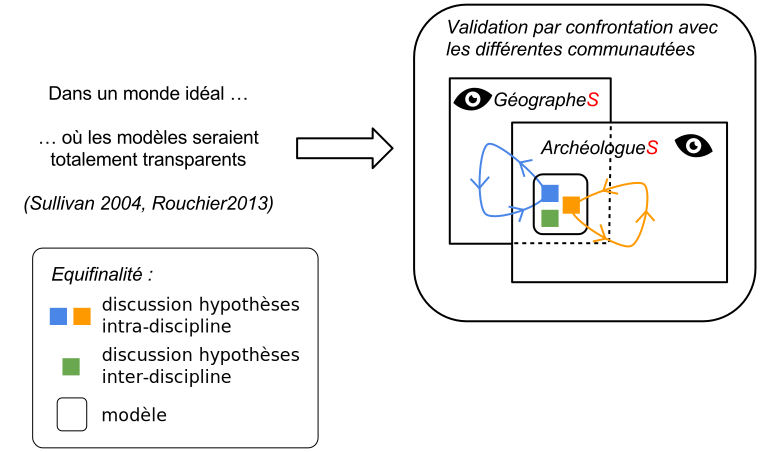
\includegraphics[width=0.9\linewidth]{vconfrontation.pdf}
  \end{sidecaption}
\end{figure}

Dans un \enquote{monde idéal}, où les modèles seraient totalement transparents (c'est-à-dire sans erreur, et dont la dynamique interne générale et propre à chaque hypothèse est complétement connue, voir figure \ref{fig:S_vconfrontation}) alors reste seulement en discussion les hypothèses, les implémentations d'hypothèses, et les critères d’évaluation choisis pour figurer au coeur du modèle. L’équifinalité impose donc qu’une partie de la validation (dont on sait qu’elle est contextuelle) s'opère dans cette confrontation avec les autres acteurs, et donc les autres points de vue de la communauté.

Ainsi plus que les solutions techniques qui restent avant tout des moyens, c'est dans le processus de discussion et d'échange autour des hypothèses et des critères admis dans les modèles que notre connaissance sur les phénomènes réels est aussi amenée à progresser. Cette confrontation n'est pas statique, elle mobilise aussi une relecture des raisonnements ayant porté l'intégration des hypothèses ou des critères au modèle. %Ce n'est qu'à ce prix que des discussions à même de susciter la modification, l'hybridation et donc l'amélioration de ces mêmes modèles peuvent être mis en oeuvre.

C'est exactement ce que nous dit \textcites{OSullivan2004,Millington2012}, il faut aller plus loin et donner toute ses chances à cette discussion, en exposant le raisonnement, et les discours développés avec et autour des modèles :

\foreignblockquote{english}[\cite{OSullivan2004}]{The process of model development, the possible outcomes it reveals and interpretations of those outcomes, taken together, constitute a geographical narrative, so that modellers become ‘makers’ of stories.}

Si l'on se place sur le plan de la reproductibilité, moins exigente et pourtant encore peu mise en oeuvre cette dernière décennie \autocite{Wilensky2007a}, l'objectif porté par O'Sullivan nous impose d'aller encore plus loin en permettant aussi la reproduction des raisonnements accompagnant la construction des modèles. La variabilité exposée lors de la construction du modèle, les différentes hypothèses, les différents critères, le jeu de leur mise en tension réciproque, tout cela devient partie intégrante d'une capsule temporelle autonome et reproductible qui peut être exportée, rejouée, modifiée, discutée auprès des autres modélisateurs \Anote{horizon_naif}. De ce fait cette confrontation avec la propriété d'équifinalité des systèmes complexes passe d'une explicitation souhaitée pour l'interdisciplinarité, à une explicitation plus que souhaitable, voire nécessaire pour la reconstruction et la discussion des raisonnements produits. Associé à la cumulativité et en donnant à voir autant ce qui marche, que ce qui ne marche pas dans nos modèles, on offre aussi cette possibilité d'une progression commune dans la déconstruction d'une partie de cette équifinalité. Comme le propose Denise Pumain, il s'agit de construire et de \enquote{défendre un projet unifié de quête d'intelligibilité} pour les sciences \autocite[157-158]{Mathieu2014}.

Seulement jusqu'à présent l'évaluation des modèles n'est pas censée avoir de sens une fois sortie de son contexte de création, il y a donc un effort évident à faire pour se doter de l'ensemble des moyens nécessaires à l'exposition de ce contexte. La notion de \enquote{laboratoire virtuel} traditionnellement limitée à l'expérimentation du modèle mute, se pare aujourd'hui d'une acception légèrement différente. Des chercheurs \autocites{Schmitt2014, Amblard2003} ont voulu étendre cette notion pour y inclure également l'ensemble des méthodes et outils jugés nécessaires à l'étude de ce premier niveau d'expérimentation que représente la construction d'un modèle de simulation (la variation des hypothèses dans le modèle), désignant par ce fait un niveau supplémentaire d’expérimentation (la variation des outils et méthodes pour construire et étudier le modèle). Il faut encore étendre et repenser l'analogie du \enquote{laboratoire virtuel}, faire de celui-ci une \enquote{place publique} et lui donner une profondeur temporelle afin de rejouer, en tout transparence, la construction des modèles au contact des données, des critères, des expérimentations \foreignquote{latin}{in vivo}.





\paragraph{Le poids du temps et du contexte }
\label{p:poids}


%Abduction, temporalité des hypothèses

L'abduction suggère que plusieurs hypothèses alternatives puissent se manifester à chacune des étapes marquant le raisonnement. La destination de celles-ci n'est pas prévisible à l'avance, et reste fonction de ce qui s'est passé précédemment dans le fil du raisonnement, c'est-à-dire les expérimentations précédentes. Comme l'indique \textcite{Besse2000} \enquote{nous ne sommes pas dans une logique de la preuve. On nous propose plutôt d'envisager l'ensemble des démarches par lesquelles les chercheurs s'\textit{orientent} vers les hypothèses qui semblent plausibles, en éliminant celles qui ne peuvent être considérées comme pertinentes.} Ainsi, il peut donc tout à la fois s'agir de conforter une précedente construction, ou justement tenter de la mettre en difficulté. Ce n'est pas d'ailleurs parce que l'on a décidé de mettre en avant l'une ou l'autre de ces stratégies dans la sélection des hypothèses et/ou des critères devant en rendre compte que ce souhait va se réaliser durant la simulation. C'est justement tout l'intérêt de l'expérimentation que de confronter la réalité de cette dynamique aux formes de nos a priori (hypothèses ou critères).

Une façon de sélectionner de façon plus efficace les hypothèses est proposée par \textcite[300]{Cottineau2014b} dans une \foreignquote{english}{proof of impossibility} :

\blockquote[{\cite[300]{Cottineau2014b}}]{[...] si la simulation n’est pas capable de fournir de \enquote{ preuve de possibilité } suffisamment restrictive pour garantir une explication convaincante, elle serait à même de fournir des « preuves d’impossibilité », lorsqu’un jeu de mécanismes s’avère inapte à reproduire les régularités recherchées. Ainsi, la qualification d’une hypothèse en soi ne peut pas être définitive et s’arrête à la possibilité, tandis qu’une disqualification de modèle est possible (lorsqu’elle est appuyée sur une exploration intensive et des tests de robustesse), et permet un retour théorique. Cette force de la falsification par rapport à la corroboration était l’argument de K. Popper (1973) pour la validation — plus large — des théories scientifiques.}

Inspiré par le \foreignquote{english}{proof of possibility} de Petri Ylikoski et Caterina Marchionni \autocite{Marchionni2013}, cette forme de falsification \Anote{idee_refutation} semble apporter un regain de causalité de façon locale au modèle car elle permet de renforcer la crédibilité des hypothèses avancées les unes par rapports aux autres.

\medskip

\textit{Est-ce pour autant qu'une hypothèse peut être écartée définitivement ?}

\medskip

Si l'on en croit \textcite[17]{Besse2000}, pas vraiment, car cela serait oublier qu'\enquote{une hypothèse possède une signification propre, avant même d’avoir été engagée dans l’aventure hautement improbable des programmes de Validation.} Certaines hypothèses peuvent être mobilisées parce qu'elles sont déjà porteuses d'un sens préalable. C'est la même chose pour les critères, qu'ils soient qualitatifs ou quantitatifs eux aussi tiennent d'une modélisation, et donc d'une construction. Par exemple, \textcite[80]{Schmitt2014} a listé une dizaine de faits stylisés pouvant être mobilisés dans le cadre d'une étude de la dynamique des systèmes de villes. Ce contexte de travail n'est pas figé, les critères et les hypothèses ne sont pas forcément connus à l'avance. L'activité de construction et de mobilisation des critères permettant de questionner le modèle lors de sa construction révèle aussi une autre activité de modélisation, aussi questionnante et importante que la construction des hypothèses puisque c'est par ce biais que les questions sont posées au modèle. Les deux activités pourraient même apparaître comme indissociables, la complexification des modèles appelant fort probablement l'introduction toujours plus grande de critères pour en mesurer la cohérence interne.

Or, s'il est courant d'établir un modèle conceptuel pour cristalliser un jeu d'hypothèses à mobiliser dans une simulation, la planification d'une grille de critères thématiques à construire et/ou à mobiliser pour mesurer de façon plus ou moins sélective les capacités de la dynamique du modèle aux différentes étapes de sa construction est nettement moins courante, et pourtant celle-ci semble tout autant nécessaire (la figure \ref{fig:S_criterecottineau} extraite de la thèse de \textcite{Cottineau2014b} propose une illustration crédible d'un tel projet).

\begin{figure}[htbp]
\begin{sidecaption}[Grille de critères utilisée par Clémentine Cottineau pour la famille de modèles MARIUS]{Grille synthétisant et ordonnant les critères utilisés pour évaluer et classer les différents modèles de la famille MARIUS construits de façon progressive dans la thèse de \textcite[329]{Cottineau2014b} : \enquote{Étant donnée la question de recherche posée aux modèles et leurs niveaux variables de complexité et de particularité, cette sélection s’organise de manière hiérarchique selon un gradient de particularité, et selon un gradient de difficulté du critère à remplir, correspondant à une distinction entre critères macro-géographiques (plus aisés car agrégés) et critères micro-géographiques (plus difficiles à reproduire dans leur diversité)}.}[fig:S_criterecottineau]
  \centering
 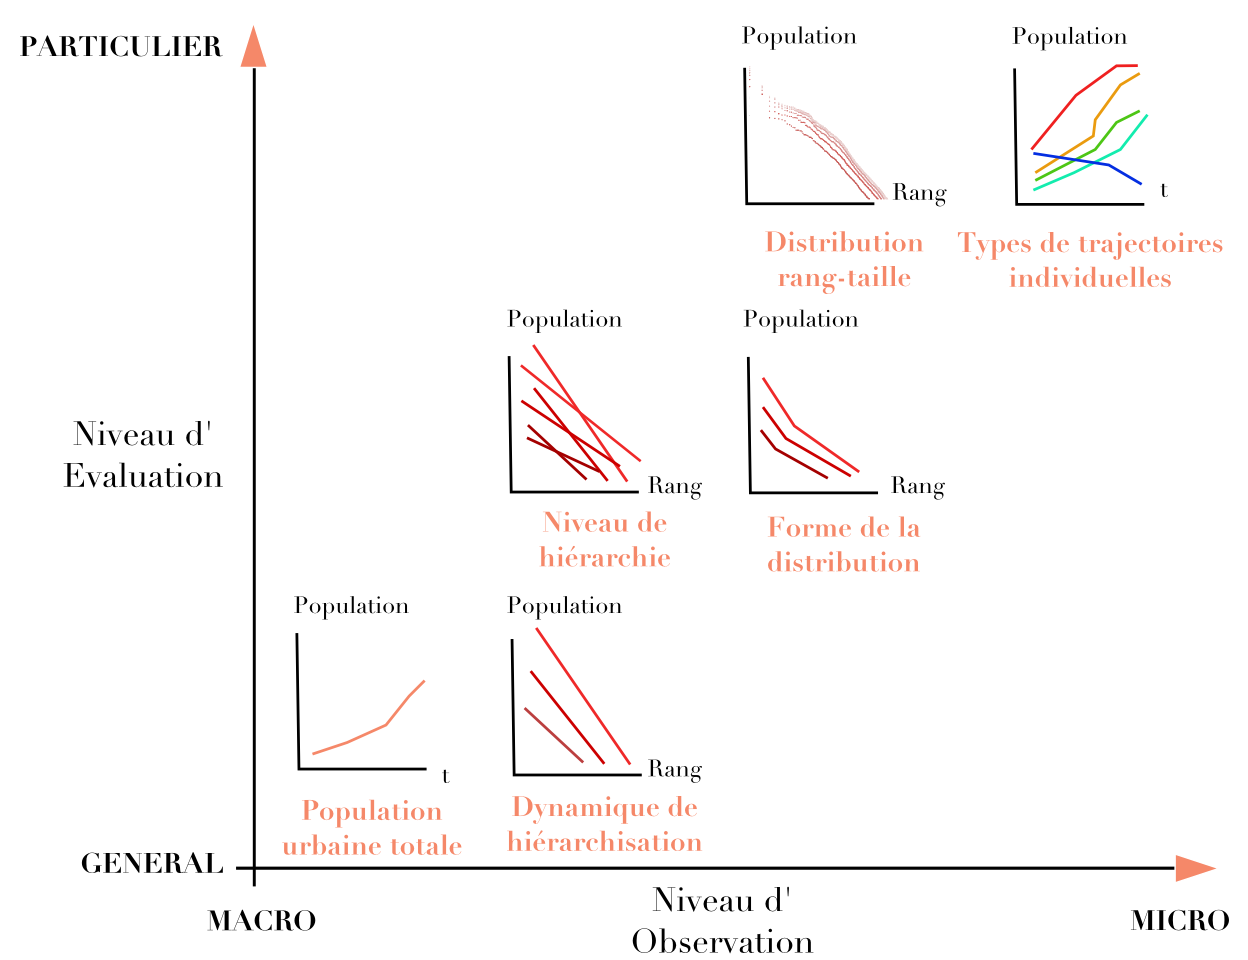
\includegraphics[width=.9\linewidth]{grideval.png}
  \end{sidecaption}
\end{figure}

D'un autre côté, l'activité abductive, même si elle paraît se concentrer initialement sur la construction du modèle de simulation, ne s'applique pas qu'à celui-ci, car le modèle de simulation n'est qu'un rouage de plus mobilisé -pour ses capacités spécifiques- dans une chaîne de traitements, dans une démarche de construction des connaissances plus globale. Les géographes ont su cumuler les avantages spécifiques des outils au fur et à mesure qu'ils ont pu intégrer la discipline. Il faut prendre un certain recul, et voir que la construction d'un modèle de simulation s'insère dans une chaîne de traitements ouverte comptant plusieurs autres modèles, eux aussi potentiellement en construction, et dont l'articulation tient également d'un raisonnement. Dans son analyse sur la place de l'explication en analyse spatiale, \textcite{Sanders2000} voit d'ailleurs plus dans le rapport de l'outil à la démarche adoptée (exploratoire ou hypothético-déductive) une question d'interprétation. \enquote{Ce sont en effet la manière dont l'outil est inséré dans une chaîne de réflexion et de traitement et l'interprétation des informations figurant en entrée et en sortie qui permettent de donner le statut descriptif ou explicatif d'une démarche.} Avant de conclure un peu plus loin à la fin de son analyse \enquote{[...] il n'y a pas de relation simple et fixe, ni entre les niveaux d'observation et la nature des explications, ni entre les outils de l'analyse spatiale et l'explication. La variété des approches permet de diversifier les éclairages sur les phénomènes que l'on cherche à expliquer. Nos démarches en analyse spatiale consistent ainsi davantage à \enquote{éclairer} qu'à \enquote{démontrer} et identifier des jeux de causalités bien stricts.} Selon Lena Sanders, la démarche généralement adoptée en analyse spatiale fait donc figure d'intermédiaire, et les aller-retour entre approches exploratoires et approches plus déductives se rapprochent selon elle de cette démarche abductive décrite par Besse.

A travers l'activité de modélisation, c'est donc toute une chaîne de modélisations qui est appelée pour faciliter cette progression du raisonnement vers la résolution de la problématique initialement posée. La découverte au cours de l'exploration du modèle d'une forte dépendance dans l'expression dynamique de certaines hypothèses peut très bien inciter le modélisateur à explorer de nouveau ces données pour questionner l'existence empirique d'une telle corrélation. On peut également déduire de la découverte de nouveaux motifs dans l'exploration d'un jeu de données (permises par exemple par l'utilisation de nouvelles techniques exploratoires) de nouvelles hypothèses dont on va tester les effets dans un modèle de simulation. Par conséquent les expérimentations, qu'elles soient sur un modèle ou sur un autre, sont susceptibles de se répercuter de façon imprévisible sur toute la chaîne de traitements. Comme le précise \textcite[63]{Mathian2014}, \enquote{Les pratiques sont telles dans le domaine du traitement des données géographiques, qu'aucune démarche n'est la suite linéaire d'une série d'étapes. C'est une combinaison de constructions de modèles de différents niveaux (modèle de données, modèle d'analyse spatiale, modèle statistique, représentations visuelles, modèle de simulation).}

Les avantages et les inconvénients de chacun des modèles, et la flexibilité de leurs relations dans ce qui constitue un véritable système de modèles pour \enquote{représenter, et comprendre l'évolution des phénomènes sociaux et environnementaux inscrits dans l'espace} sont très bien encadrés par les écrits des géographes \textcites{Sanders2000, Mathian2014}. On trouve dans la thèse de \textcite{Cottineau2014a, Cottineau2014b} un travail décrivant de façon très précise les inter-relations fructueuses entre une activité de construction de modèles de simulation et d'autres types de modélisations (statistiques, spatiales).

%et renvoie en alternance aux données et aux modèle de données, qui elle même renvoie aux hypothèses et aux implémentations de ces hypothèses, aux indicateurs et à la façon dont on les a construit, etc.

%De nouveau, on constate l'importance du contexte, et l'impossibilité de s'en détacher \autocite{Amblard2006}.

Si les hypothèses et les critères se construisent et se vérifient pour partie dans un espace-temps qui peut s'avérer très différent de celui mobilisé par et pour la seule simulation, est-il possible d'identifier durant la construction d'un modèle de simulation le moment idéal de leur introduction ? C'est peu probable, et ce n'est pas cette seule conceptualisation en amont de la construction des modèles qui pourra nous en assurer, car cela reviendrait à confondre la dynamique réelle et complexe d'interactions non linéaires entre hypothèses au sein du modèle avec celles que l'on a imaginées et projetées sur le papier. Il faut ainsi garder en mémoire que cette dynamique se soucie assez peu du sens que l'on a bien voulu rattacher aux hypothèses, aux paramètres que l'on introduit, ou que l'on décide d'introduire à un instant $t$ dans nos constructions. Cette conceptualisation en amont reste évidemment un guide important qui permet de formaliser cette expérimentation.

Comme il est relativement difficile de se projetter dans une telle dynamique de construction, on peut essayer d'exemplifier un peu mieux les questions qui peuvent se poser avec l'introduction (ou le retrait) des hypothèses/critères dans les modèles.

On propose la construction d'un modèle de simulation KISS suivant une trajectoire classique de complexification dont la finalité importe peu dans cet exemple. La première implémentation visée est celle d'un modèle \textit{null theories} \autocite{Railsback2012}. Comme son nom l'indique, l'objectif est de commencer au plus tôt la phase de construction/expérimentation avec un modèle de simulation mobilisant le moins d'hypothèses/critères possible. L'objectif de cette construction est double.

Une première opérationnalisation, même minimale, permet de mettre en évidence la dépendance du modèle conceptuel vis-à-vis du modèle implémenté. Il n'est pas problématique d'avoir un modèle conceptuel détaillé dès le départ, au contraire, mais si l'on décide de réaliser un modèle de simulation, il faut toujours avoir à l'esprit que c'est de l'expérimentation que dépend la progression du raisonnement. Plus vite celle-ci est mise en marche, plus vite on peut entamer cette progression. Cela permet aussi de ne pas minorer l'étape d'implémentation des hypothèses, qui soulève à elle seule des premières divergences avec le modèle conceptuel. La construction d'un premier modèle aux hypothèses minimales permet aussi de connaître le poids interprétatif attribuable à la structure du modèle ainsi mis à nu. Ce qui permet d’observer dans l’évolution du modèle, quel est l’apport exact de chaque nouvelle hypothèse, ou de chaque nouveau critère dans la dynamique exprimée du modèle.

Les hypothèses et les critères mobilisables durant l'activité de modélisation sont tout à la fois des construits qui émergent de cette chaîne de traitements plus globale qui supporte la progression du raisonnement, que des éléments empruntés d'un catalogue plus général, hérités de plusieurs décennies de modélisations en géographie et vérifiés de multiples fois par l'empirie (le modèle gravitaire, la loi rang-taille, etc.).

Les hypothèses et les critères mobilisés supportent de façon implicite des valeurs différentes, qui n'apparaissent pas forcément comme évidentes d'un point de vue extérieur. Il est difficile par exemple d'éliminer une hypothèse en fonction de sa seule mise en défaut observée à un instant $t$ dans la construction d'un modèle, d'autant plus lorsque la présence de celle-ci dans le modèle a du sens dans la résolution d'une problématique.

Peut-être n'était-ce simplement pas le moment pour intégrer cette hypothèse au modèle, celui-ci étant encore trop simple ? Peut-être faut-il activer ou implémenter d'autres hypothèses pour que celles-ci puissent se révéler ? Peut-être que le critère devant rendre compte de cette dynamique n'est pas suffisamment adapté ? Peut-être que l'implémentation proposée n'était tout simplement pas la plus pertinente compte tenu de la dynamique déjà existante ? Peut-être que l'entité choisie pour porter l'hypothèse ne se situe pas à la bonne échelle ? etc.

Inversement une hypothèse ou un critère valable à un instant $t$ ne le sera peut-être plus à un instant $t + 1$. L'explication et la mise en place cohérentes des hypothèses et des critères se fait donc dans ces aller-retour, dans ces multiples essais. La construction d'un modèle de simulation ne semble pas tenir d'un raisonnement linéaire, car les interactions entre le modélisateur et le modèle sont complexes, et opèrent, comme on le perçoit dans toutes ces questions, à de multiples niveaux, parfois de façon simultanée.

\begin{figure}[htbp]
	\begin{sidecaption}[Exemple d'une démarche de construction cumulative]{Exemple d'une démarche de construction cumulative}[fig:S_cumulative]
	 \centering
	 \subbottom[Pendant la construction d'un modèle (\textit{building step}) ce sont différentes hypothèses (ici $A$ et $B$) et différentes versions d'hypothèses (ici versions $\{A_1 \dotsc A_n\}$ et versions $\{B_1 \dotsc B_n\}$) qui vont être développées. Si on veut mettre en oeuvre une approche cumulative et mobiliser toute la combinatoire possible entre les différentes versions des hypothèses implémentées durant la construction du modèle, alors il faut considérer la création d'un graphe de dépendances (\textit{graph dependency}). On s'aperçoit alors que certaines versions des hypothèses ne sont pas compatibles les unes avec les autres (ex $A_1$ avec $B_2$). Les figures \ref{fig:S_twomeca} et \ref{fig:S_buildmeca} proposent d'instancier cet exemple dans deux familles d'hypothèses régissant les échanges d'innovations entre des villes dans un système de villes.\label{fig:cumulative_a}]{
	 	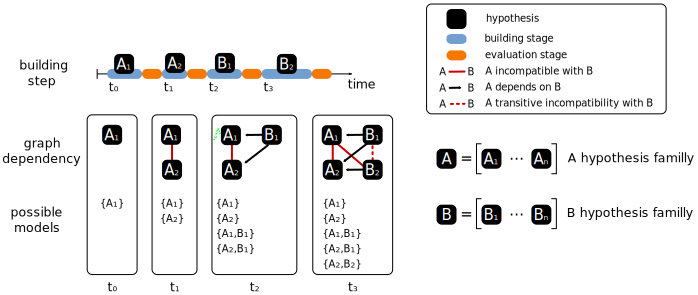
\includegraphics[width=1.0\linewidth]{schema_dependency.pdf}
	 	}\qquad
	 \subbottom[On propose d'étudier plusieurs hypothèses décrivant la façon dont une ville (la ville $i$) peut récupérer et intégrer dans son propre \textit{pool} d'innovations les innovations échangées avec les villes voisines pendant la simulation. Deux niveaux d'hypothèses sont imaginables. Le premier niveau d'hypothèse, le plus simple, propose d'intégrer les innovations à la ville $i$ à chaque fois qu'un échange a lieu avec une ville $j$. C'est la famille $A$ dont on trouve deux versions implémentées dans la figure \ref{mechanisme1}. Un deuxième niveau d'hypothèse est envisageable, plus complexe et dépendant du premier niveau il mobilise deux étapes représentées dans la figure \ref{mechanisme2} : 1) on considère l'ensemble des échanges possibles entre la ville $i$ et ses voisines, 2) l'ensemble d'innovations résultant de ces échanges est ensuite filtré puis intégré à la ville $i$ en fonction des règles définies par la famille d'hypothèse $B$ \label{fig:S_twomeca}]{
		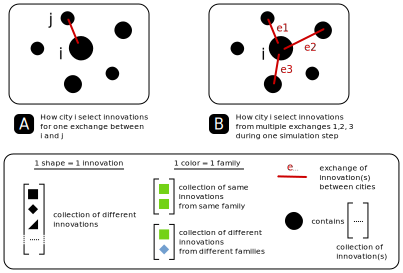
\includegraphics[width=0.8\linewidth]{mechanismslocal.pdf}
		}
	\end{sidecaption}
\end{figure}

\begin{figure}[p]
	\begin{sidecaption}[Exemple d'implémentations de plusieurs familles d'hypothèses]{Présentations des implémentations et des inter-dépendances entre ces implémentations dans le cas des deux familles d'hypothèses $A = \{A_1,A_2\}$ et $B = \{B_1, B_2\}$}[fig:S_buildmeca]
	 \centering
	 \subbottom[Les versions $A_1$ et $A_2$ mobilisent chacune des règles très différentes pour définir la règle de sélection et d'intégration de l'objet innovation échangé entre deux villes $i$ et $j$. La couleur est en effet introduite comme une nouvelle propriété des innovations dans la deuxième version $A_2$ de cette hypothèse $A$.\label{mechanisme1}]{
	 	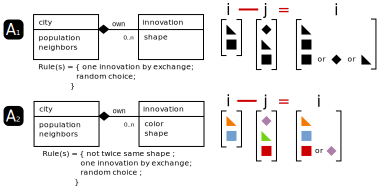
\includegraphics[width=0.9\linewidth]{a1a2mechanism.pdf}
	 	}\qquad
	 \subbottom[Les deux familles de mécanismes sont assemblées en fonction du graphe de dépendance déjà présenté dans la figure \ref{mechanisme1} : $A_1$ est compatible avec $B_1$, mais pas avec $B_2$ car la propriété couleur des innovations est nécessaire à son bon fonctionnement. Les mécanismes $B_1$ et $B_2$ sont par contre tout à fait compatibles avec la version $A_2$. \label{mechanisme2}]{
		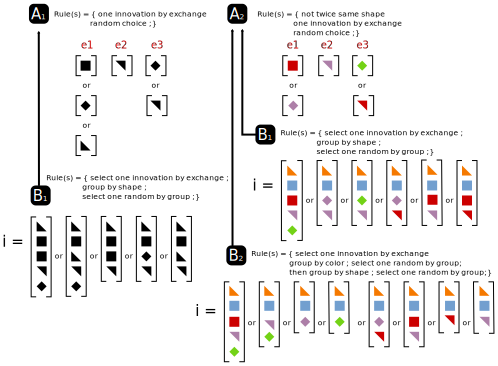
\includegraphics[width=1.0\linewidth]{a1a2b1b2mechanism.pdf}
		}
	\end{sidecaption}
\end{figure}


\begin{figure}[htbp]
\begin{sidecaption}[Evaluation automatique des hypothèses face à des critères multiples]{Les différentes versions des mécanismes sont assemblées dès lors qu'elles sont compatibles (voir le schéma \ref{fig:S_buildmeca}). Les modèles de simulation ainsi assemblés sont évalués face aux multiples critères experts (qualitatifs, quantitatifs) mobilisés durant la construction. L'hypothèse $A_1$ utilisée à $t_0$ toute seule donne de meilleurs résultats que l'hypothèse $A_2$, plus complexe et construite a $t_1$. Il pourrait être tentant d'écarter de suite cette hypothèse, qui reste inférieure à l'hypothèse $A_1$, même une fois couplée à $B_1$ ($\{A_2,B_1\} < \{A_1,B_1\}$). Une fois associée après la phase de construction $t_3$ à la version $B_2$ de l'hypothèse $B$, c'est pourtant la seule combinaison $\{A_2,B_2\}$ qui permettra de satisfaire à la fois le critère 1 et 2.}[fig:S_critererempli]
  \centering
 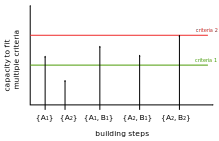
\includegraphics[width=.8\linewidth]{capacity.pdf}
  \end{sidecaption}
\end{figure}

Comme nous nous situons depuis le début dans une problématique de calibrage par optimisation, dont les résultats n'ont pas vocation à être transférés de façon directe à une situation réelle, l'apparition d'un nouveau critère venant contraindre la dynamique peut complétement \enquote{changer la donne} dans cette combinatoire des hypothèses plausibles. Interpréter de telles situations peut rapidement devenir très complexe : 3 hypothèses peuvent produire une dynamique plus proche des critères que 2 hypothèses, mais 1 hypothèse seule peut apparaître meilleure que trois hypothèses sur ce même objectif.

Peut-être que la combinaison de ces deux hypothèses est ici la plus intéressante du point de vue des questions thématiques qu'elle pose, et cela même si la combinaison des trois hypothèses produit de meilleurs résultats. Peut-être qu'à l'introduction d'un nouveau critère, la solution à deux hypothèses produira des meilleurs résultats, et que l'hypothèse 1 verra ses résultats se dégrader ?

Cette interpretation dépend donc du degré de complexification du modèle au moment où on l'évalue, du nombre de critères retenus pour juger la dynamique de celui-ci, et de la valeur relative que l'on attribue à chacune de ces hypothèses. La figure \ref{fig:S_critererempli} essaye d'exemplifier un tel scénario en s'appuyant sur l'exemple de modèle simplifié présenté dans la figure \ref{fig:S_buildmeca}. Par conséquent aussi cette possibilité de falsification ou \foreignquote{english}{proof of impossibility}, ne marche que si l'on est en mesure de prouver l'\textbf{inaptitude constante} d'une d'hypothèse ou d'un jeu d'hypothèses dans la confrontation avec les critères d’évaluation. Il reste donc à gérer cette possibilité de réengager les hypothèses et les critères à différents moments dans la construction des modèles, et soutenir une activité de construction cumulative (voir la figure \ref{fig:S_cumulative}) qui ne soit pas \enquote{oublieuse} de cet autre espace-temps dans lequel se construisent les hypothèses et les différents critères mobilisés.


\paragraph{Montrer l'équifinalité dans l'évaluation des modèles}
\label{p:nvlle_equifinalite}

Là où le premier cadre d'analyse amené par les sociologues propose de réaffirmer le statut explicatif des hypothèses insérées dans les modèles par un ancrage empirique plus important de celles-ci, et une épistémologie admettant l'existence possible d'une explication même si la chaîne de causalité s'avère lacunaire, nous avons suivi une toute autre trajectoire dans notre équipe, qui semble répondre aussi aux enjeux présentés dans les paragraphes précédents.

Il a en effet été choisi de justifier cette équifinalité non pas en l'intégrant dans un nouveau cadre d'analyse, mais en la faisant plutôt apparaître de façon explicite comme le résultat de nos démarches de raisonnement accompagnant la construction des modèles. Il ne s'agit plus de produire des modèles de simulation comme des instances finalisées d'un raisonnement dont on ne verra jamais la construction, mais des modèles conçus comme la réalisation de trajectoire dans une famille d'hypothèses et de critères qui intègre et donne à voir cette variabilité et ces aller-retours possibles dans les propositions.

L'idée de fabriquer des familles d'hypothèses et de critères capables de supporter le développement de réponses non linéaires face aux données présentées n'est pas neuve dans la discipline. Certains géographes ont même présenté de façon très précoce des solutions techniques pour fabriquer et évaluer de façon automatique des modèles à partir d'un corpus initial d'hypothèses \autocite{Openshaw1988}.

Il y a, je crois, plusieurs avantages à voir dans cette solution.  Elle permet de supporter la transformation des modèles dans le temps et dans les disciplines, tout en offrant le support d'un cadre de discussion idéal pour penser l'interdisciplinarité.

Il peut y avoir aussi des inconvénients, car même dans sa version la plus simple, cette solution nécessite pour être opérationnalisée des efforts conséquents, expliquant aussi pourquoi de telles plateformes n'ont existé que sous la forme de prototype.

\begin{itemize}
\item Supporter une évaluation rapide et systématique des modèles construits face aux critères selectionnés
\item Supporter la formalisation des interdépendances entre hypothèses, paramètres, et critères
\item Encapsuler et versionner les données
\item Encapsuler et versionner les différents modes d'exploration du modèle
\end{itemize}

%Si on comprend les enjeux d'un tel projet, se pose alors les moyens de sa réalisation; la systématisation des évaluations avait déjà été annoncé comme un outil devant être mobilisé dès la pose des premières hypothèses, mais elle devient absolument nécessaire pour rendre cette fouille de modèles réaliste, et passé peut être à une échelle supérieure, celle de la construction et de l'étude de famille de modèles comme premier élément de réponse intégrateur de la pluralités des points de vues.


% Ce qui a mon sens soulève ici plusieurs remarques :
% - il est vraiment difficile de savoir ce qui va se passer avec l'intégration ou le retrait des hypothèses, ou des critères d'évaluation dans un modèle de simulation si on ne dispose pas d'un outil permettant d'évaluer systématiquement chacune de ces modifications, ce point est valable tout autant pour les approche KIDS que KISS.
% - cette évaluation doit être mis en place de façon immédiate, dès que les premières questions sont posés à la structure causale du modèle, afin de ne pas biaisé le raisonnement construit par la prolongation d'une phase de \textit{face validity} pouvant très vite devenir problématique de part les redéveloppements qu'elle suppose dans le futur.
% - malgré cela, il faut bien voire qu'une exploration des comportements du modèle, même complète, ne fera pas disparaitre ce problème, qui tient avant tout de l'avancement du raisonnement dans la construction du modèle.



\printbibliography[heading=subbibliography]

\stopcontents[chapters]

% -*- root: These.tex -*-
\graphicspath{{FigurePartie2/}}

\chapter{Réalisation d'une plateforme intégrée}

\startcontents[chapters]
\Mprintcontents

% -*- root: These.tex -*-

\Anotecontent{versionnerwf}{Par versionner on entend a minima la possible de  garder, de visualiser, de restaurer l'ensemble des modifications apportés à un fichier ou un ensemble de fichier. Les \textit{workflow} contiennent des données de natures très hétérogènes (modèles de simulation, bases de données, fichiers, etc.), ce qui rend le développement d'un outil capable de stocker et de restaurer intelligement un tel environnement dans ses différentes versions plus complexe à réaliser.}

\Anotecontent{ca_calibrage}{Cette littérature semble émerger, en géographie, plus vite dans le calibrage automatique des CA que dans la calibration des ABM.}

\Anotecontent{pom_realiste}{\foreigntextquote{english}[{\cite[315-316]{Railsback2012}}]{Let us warn you that no other platforms or ways to design and program ABMs are remotely as easy to use, well documented, and polished as Netlogo is. You can expect a serious increase in the effort and software knowledge required to produce working models, which could be a strong incentive to keep your models simple enough to stick with netlogo. However, if you do think you will outgrow NetLogo, we strongly recommend taking one or two serious courses in object-oriented programming, probably using the Java language.[...] Another alternative to consider seriously is finding a collaborator to provide the software expertise - either a paid programmer or an academic computer scientist (Chapter 8 of Grimm and Railsback 2005 provides advice on working with software professionals.)}}


\Anotecontent{paul_rationalite}{On parle aussi de rationalité procédurale dans le domaine de la cognition.}

\Anotecontent{uncertainty_grimm}{\foreigntextquote{english}[{\cite[255-256]{Railsback2012}}]{Parameterization is the word modelers used for the step of selecting values for a model's parameters.[...] The reason that parametrization is important is, of course, that quantitative results matter.[...] Calibration is a special kind of parameterization in which we find good values cause the model to reproduce patterns observed in the real system. Calibrating an ABM is part of POM because we calibrate \enquote{against} (i.e., to reproduce) patterns observed in the real system. Now, however, the patterns are typically quantitative instead of qualitative and more descriptive of the whole system, not its agents and parts. [...] Why do we include calibration as a part of pattern-oriented modeling separate from theory development, when they both include changing of adjusting a model until it adequately matches a set of observed patterns ? The major differences is that in theory development, we are focused on one particular part of a model: its traits for agent behavior. We often test theory against qualitative patterns so that we do not need to worry yet about how closely model reproduces observations from the real system. Calibration comes after we've identified theory for behavior and assembled the full model. Another way to think of the difference between this chapter and the rest of POM is that chapters 18 and 19 were about using patterns to reduce a model's \enquote{structural uncertainty} by finding good model designs and agent traits, and this chapter is about reducing \enquote{parameter uncertainty} by finding good parameter values.}}

\Anotecontent{evaludation}{\foreigntextquote{english}[\cite{Augusiak2014}]{Confusion about model validation is one of the main challenges in using ecological models for decision support, such as the regulation of pesticides. Decision makers need to know whether a model is a sufficiently good representation of its real counterpart and what criteria can be used to answer this question. Unclear terminology is one of the main obstacles to a good understanding of what model validation is, how it works, and what it can deliver. Therefore, we performed a literature review and derived a standard set of terms. ‘Validation’ was identified as a catch-all term, which is thus useless for any practical purpose. We introduce the term ‘evaludation’, a fusion of ‘evaluation’ and ‘validation’, to describe the entire process of assessing a model’s quality and reliability.}}

\Anotecontent{dsl}{Pour les modélisateurs, il faut imaginer que ce langage dédié met à disposition des utilisateurs différentes primitives spécifiques au logiciel pour construire et exécuter les \textit{workflows}, un peu comme Netlogo le propose avec la manipulation des Tortues.}

\Anotecontent{holland_multi_utilisation}{ Holland a développé les GA avant tout pour leur capacité de \foreignquote{english}{robust adaptive systems} et pas seulement pour leur capacité d'optimisation comme le rapelle \textcite{DeJong1993a} : \foreignquote{english}{However, with all this activity, there is a tendency to equate GAs with function optimization. There is a subtle but important difference between \enquote{GAs \textbf{as} function optimizers} and \enquote{GAs \textbf{are} function optimizers}} ; L'investissement d'Holland dans l'étude des \foreignquote{english}{Complex Adaptive Systems} s'inscrit dans une trajectoire de recherche resté proche des thématiques de ce qui deviendra plus tard la méta-discipline \textit{Artificial Life}. Son investissement continue dans cette branche de développement est d'ailleurs lisible au travers de plusieurs créations de plateformes sur ce thème : \textit{$\alpha$-universe} et \textit{Echo} dont on trouve une analyse dans les travaux de \autocites{Taylor1999, Taylor2001} }


\Anotecontent{difference_objective_heuristique}{Il n'est pas forcément évident de faire la différence entre ces termes très proches, dont le sens se recoupe parfois, voici donc une aide à la désambiguisation inspirée de celle de \textcite[36]{Weise2011} :

\begin{enumerate}[labelindent=\parindent,leftmargin=*]
\item La fonction objectif (\textit{objective function}) peut etre considérée comme une forme d'heuristique, à la différence que celle ci est une mesure forcément directe du potentiel d'un aspect de la solution, alors que l'heuristique peut être de mesure directe ou indirecte, en ne fournissant par exemple qu'une approximation de la distance séparant une mesure de l'optimum. En ce sens, la fonction objectif mobilise souvent plus d'expertise sur le système que l'heuristique.
\item Une fonction \textit{fitness} est une fonction d'utilité secondaire, conçue comme une combinaison possible de fonction objectifs, et/ou d'heuristiques. Celle-ci peut également être une mesure relative, pour quantifier par exemple la différence existante entre deux solutions.
\end{enumerate}}

\Anotecontent{barricelli_multi_utilisation}{ Tout comme les travaux de McMillan ont permis de voir plus clair dans les intentions de Von Neumman derrière la notion de \textit{self-reproduction automata} ..., les travaux de Dyson \Autocite{Dyson1997}, de Fogel \autocite{Fogel2006a} sur l'histoire de cette discipline a permis également de redécouvrir les recherches de Barricelli comme celle d'un véritable pionnier en ALife, mais également comme celui d'un pionnier dans l'idée d'utiliser l'évolution comme support à la résolution de problème.}

\Anotecontent{fraser_comment}{\foreignquote{english}{Fraser was one of the first to conceive and execute computersimulations of genetic systems, and his efforts in the 1950s and1960s had a profound impact on computational models of evo-lutionary systems. The simulation algorithms he used were im-portant not only in the simulation of genetical problems, but pro-vided a menu of techniques that enriched the entire simulationeffort in any problem that involved probability sampling amonga population of alternatives, the heart of Monte Carlo methods. }\autocite[429]{Fogel2002}}

\Anotecontent{note_pattee_semantic_closure}{ \foreignquote{english}{Additionnary, from an epistemological point of view, Pattee(1995b) points out taht symbolic information (such as that contained in an organisms's genes) has \enquote{no instrinsic meaning outside the context of an entire symbol system as well as the material organization that constructs(writes) and interprets(reads) the symbol for a specific function, such a classification, control, construction, communication ...}. He argues that a necessary condition for an organism to be capable of creative open-ended evolution is that it encapsulates this entire self-referent organisation (Pattee refers to this condition as semantic closure). From this it follows that organisms should be constructed \enquote{with the parts and the laws of an artifical physical world} Pattee (1995a)(p.36). In other words, the interpretation (phenotype) of the symbolic information (genotype) of an artificial organism should be constructed and act within the artificial physical environment of the system. Additionally, if the system is to model the \enquote{origin} of genetic information, then the genotype itself must also be embedded within the environment; that is, the complete semantically-closed organisation -- the \enquote{entire organism} -- must be completely embedded within the physical environment.} \autocite{Taylor2001}}

\Anotecontent{np_complet_def}{ \foreignquote{english}{Identifying which combinatorial problems are easy to solve and which are hard is an important and challenging task, which has occupied theoretical computer scientists for many years. In order to translate the everyday expression \enquote{easy to solve} to mathematical theory the concept of polynomial time algorithms has been introduced. An algorithm is said to run in polynomial time if there is a polynomial $p$ such that the algorithm applied to an input of size $n$ always finds a solution in time $p(n)$, that is after performing $p(n)$ simple instructions. Note that we measure the worst case complexity, that is the time in which we are sure that the algorithm ends regardless of which input of size $n$ we have fed it. The execution time of a polynomial time algorithm grows slowly enough with increasing input size to be able to be run on a computer, but if the execution time grows exponentially the algorithm is useless for all but the smallest inputs. One of the most accepted ways to prove that a problem is hard is to prove it NP-complete. If an optimization problem is NP-complete we are almost certain that it cannot be solved optimally in polynomial time.} \autocite[1]{Kann1992}}

\Anotecontent{texte_csunplugged}{Le \href{http://csunplugged.org/}{@site} officiel présente le projet ainsi : \foreignquote{english}{CS Unplugged is a collection of free learning activities that teach Computer Science through engaging games and puzzles that use cards, string, crayons and lots of running around. The activities introduce students to Computational Thinking through concepts such as binary numbers, algorithms and data compression, separated from the distractions and technical details of having to use computers. Importantly, no programming is required to engage with these ideas! CS Unplugged is suitable for people of all ages, from elementary school to seniors, and from many countries and backgrounds. Unplugged has been used around the world for over twenty years, in classrooms, science centers, homes, and even for holiday events in a park!}}

\Anotecontent{traduction_unplugged}{Le livre a été traduit par une partie de l'équipe d'\href{https://interstices.info/}{@Interstices}, et de l'EPI, il est téléchargeable à cette  \href{https://interstices.info/jcms/c_47072/enseigner-et-apprendre-les-sciences-informatiques-a-lecole}{@adresse}.}

\Anotecontent{pensee_informatique}{Le terme original \textit{Computational Thinking} vient assez logiquement de Seymour Papert et son travail sur LOGO (inspiré par quatre années passé avec Jean Piaget, l'enseignant mathématicien George Polya qui a marqué de nombreux chercheurs par sa méthode pédagogique, la rencontre avec Minsky, l'école Bourbaki, etc. \autocite{Catlin2014}) mais il a été remis au gout du jour par Jeannette Wing, directrice et professeur du département Informatique du Carneggie Melon.  \href{https://interstices.info/jcms/c_43267/la-pensee-informatique}{@traduction} en français de l'article de \textcite{Wing2006} est proposé par \href{https://interstices.info/}{@Interstices}, dont voici un extrait :
C'est le terme employé pour désigner le socle de connaissance lié à la discipline informatique, indépendamment des langages de programmation : \enquote{ La pensée informatique constitue pour nous tous un savoir fondamental, pas seulement pour les informaticiens. Au même titre que la lecture, l'écriture ou l'arithmétique, nous devrions la transmettre à nos enfants. Alors que l'imprimerie a permis la diffusion des trois premiers savoirs (lire-écrire-compter), les technologies numériques véhiculeront cette pensée informatique. Mais la situation est particulière, car c'est précisément cette pensée informatique qui a servi à développer ces technologies. Adopter un mode de pensée informatique conduit à résoudre des problèmes, à concevoir des systèmes et à comprendre le comportement humain différemment, en s'appuyant sur les concepts fondamentaux de la discipline informatique et en y incluant une panoplie d'outils intellectuels qui reflètent l'étendue de la science qu'est l'informatique.} Dans ce socle de connaissance, on trouve évidemment les principes universel d'algorithmie, de décomposition, d'abstraction, de reconnaissance de forme; mais la notion de pensée informatique va au delà, et mobilise ces concepts dans un contexte éducatif. Interviennent alors les capacités de créativité, la découverte, l'apprentissage, l'interactivité, la simulation tel qu'ils sont mobilisés dans les réflexions et les outils activateurs de cette synergie entre concept et utilisateurs tel que développés depuis les années 1970 par Papert, puis Restnick, etc.}

\Anotecontent{billet_weise}{Voir le \href{http://blog.it-weise.de/p/309}{@billet} daté de juin 2014.}

\Anotecontent{note_pengouin}{Que faut il penser par exemple d'un algorithme bio lorsqu'il est nommé \foreignquote{english}{Pengouin Search Optimization Algorithm} (PSOea) \autocite{Gheraibia2013} ? }

\Anotecontent{stochastic_note}{Si l'optimisation stochastique (\textit{stochastic optimization}) ou approche probabiliste de l'optimisation (\textit{probabilistic approaches} apparait comme un autre chapeau susceptible de pouvoir englober l'ensemble de ces techniques, le schéma \ref{fig:S_OverviewOptimisation} de Weise contredit ce constat. Il existe en effet dans cette vaste catégorie tout un ensemble de techniques (\textit{Hill Climbing}, \textit{Simulated Annealing}, etc.) qui diffèrent très fortement dans leur structure, leur définition, ou leur inspiration, de la branche de techniques qui nous préoccupe ici, à savoir l'EC. }

\Anotecontent{equipe_mixite}{Suivant les travaux menés dans notre équipe par \textcite{Reuillon2015}, la validité de ce dernier paragraphe est clairement remise en question. L'originalité de ces derniers résident dans la mixité de ces deux objectifs. En intégrant \enquote{la capacité d'extension spatiale} dans l'exploration de ces espaces comme un critère d'optimisation supplémentaire aux objectifs plus classiques de recherche de minima, une cartographie dirigée et plus exhaustive est devenue possible.}
%En intégrant l'\enquote{exploration de cette espace} des solutions (si on veut découvrir une carte  exhaustive des solutions optimisés), ou de l'espace de recherche (si on veut cartographier l'espace de recherche menant à cet espace de solution optimisé) comme un objectif d'optimisation supplémentaire aux objectifs plus classique de recherche de minima, une cartographie dirigé et plus exhaustive de certaines zones de cet espace est devenu possible.}


\Anotecontent{amoral_reproductible}{La volonté des auteurs d'une démarche exemplaire ayant vocation à être reproduite et diffusée apparaît plusieurs fois dans le manuscrit \autocite{AMORAL1983}, en introduction \enquote{Conscient de l'intérêt que cette approche modélisée par Analyse Systémique pouvait apporter, le groupe a tenu à présenter toute l'information concernant le modèle AMORAL, allant bien au-delà de sa présentation et de son mode d'emploi. Nous espérons ainsi avoir ouvert une voie qui, semble-t-il, mérite d'être explorée et expérimentée pour l'aide à la prise de décisions au niveau micro-régional.}, ou bien en conclusion : \enquote{Pour en faciliter la pratique toute l'information le concernant est accessible directement dans ce rapport : le dictionnaire de toutes les variables, tables et coefficients [...], les tables fixées en fonction des types de relations intervenant dans le modèles, le graphe complet des relations [...], le listing du programme comportant toute les équations du modèle. Cette transparence totale du travail et de ses fondements assurera peut-être une meilleur diffusion de ce rapport qui contient à la fois une approche méthodologique nouvelle pour l'aménagement du territoire, et un outil pratique d'aide à la décision.}}


\Anotecontent{amoral_note}{ La préface du rapport \autocite{AMORAL1983} et les différentes publications \autocite{Guermond1984} sur ce modèle initié avant les années 1980 sont très explicites sur l'apport méthodologique, et théorique des Systèmes Dynamiques à la Forrester. A ce sujet Marie-Geneviève Durand, alors ingénieur de recherche, raconte \enquote{Très vite, cette recherche appliquée faisant appel à une méthodologie nouvelle en la matière, nous renvoyait à la recherche fondamentale. Par voie de conséquence, le présent rapport [...] s'enrichit d'une information nécessitée par le caractère innovateur de la méthode autant que par l'utilisation du modèle. [...] Il a fallu aussi s'habituer à manipuler cette dynamique intrinsèque au système modélisé. Il en résulte un nouvel état d'esprit et une toute autre compréhension des phénomènes. Ce travail s'est donc révélé fécond, nous conduisant à réflechir sur notre propre discipline, à tester et affiner la méthode.} \autocite{AMORAL1983}}

\Anotecontent{def_meta_sorensen}{\foreignquote{english}{A metaheuristic is a high-level problem-independent algorithmic framework that provides a set of guidelines or strategies to develop heuristic optimization algorithms (Sörensen and Glover, 2013). [...] A problem-specific implementation of a heuristic optimization algorithm according to the guidelines expressed in a metaheuristic framework is also referred to as a metaheuristic. The term was coined by \textcite{Glover1986} and combines the Greek prefix meta- (metá, beyond in the sense of high-level) with heuristic (from the Greek heuriskein or euriskein, to search)} \autocites{Sorensen2013a, Sorensen2013b} }

\Anotecontent{def_meta_weise}{C'est également ainsi que \textcite[36, 225]{Weise2011} comprend ce terme \foreignquote{english}{A metaheuristic is a method for solving general classes of problems. It combines utility measures such as objective functions or heuristics in an abstract and hopefully efficient way, usually without utilizing deeper insight into their structure, i. e., by treating them as black box-procedures}}

\Anotecontent{greedy_description}{Un \enquote{choix optimal local} est réalisé à chaque itération durant l'optimisation, ce qui produit en général des solutions viables mais très rarement optimales.}

\Anotecontent{q_ppr}{Questions tirés du wiki \textit{Portland Pattern Repository} (\href{http://c2.com/cgi/wiki?MetaHeuristic}{@PPR}), qui est au passage un des premier wiki sur le web (1995)}

\Anotecontent{paysage_cumule}{En ce sens, la figure \ref{fig:spacePspaceOmultimodal} peut représenter tout autant \begin{enumerate*}[label=(\alph*)]
\item une population de solutions candidates désignées en amont par un plan d'expérience, évaluées en une seule passe par l'optimiseur, puis projetées dans l'espace des objectifs
\item ou une population cumulée de solutions candidates évaluées. C'est à dire une image à un instant $t$ représentatif du fonctionnement de l'optimiseur étalé sur plusieurs passes, celui-ci manipulant une seule solution candidate par itération. \end{enumerate*} }

\Anotecontent{test_fonction_surutilisation}{Sous l'impulsion remarquée de quelques chercheurs \autocites{Zitzler1999a, Zitzler1999b, Fonseca1996}, différentes approches ont été formalisés ces dernières années pour mieux mesurer et comparer les performances de ces différents algorithmes d'optimisation. Un travail délicat, car la nature stochastique de ces derniers rend plus difficiles les comparaisons \autocite{Coello2006}. Parmi les différents \textit{benchmark} développés on trouve par exemple : l'évaluation de \textit{set} de fonctions mathématiques (comme ceux de Schwefel et DeJong) dont on connait par avance la forme du front de Pareto \autocites[580]{Weise2011}[138]{Back1996}, l'utilisation de mesures sur les objets manipulés par ces algorithmes (par exemple des mesures sur le paysage \autocite[163]{Weise2011}, la création d'opérateurs logiques pour comparer les performances des différents algorithmes \autocite{Zitzler2003, Zitzler2007}, etc.). Depuis peu ces \textit{benchmark} sont également amenés à intégrer des plateformes permettant l'évaluation et la confrontation automatique d'algorithmes d'optimisation. C'est le cas par exemple de la plateforme COCO (\textit{COmparing Continuous Optimisers}) utilisé depuis 2009 dans les conférences GECCO \autocite{Hansen2011}. Enfin, il faut noter que certains pionniers, eux-mêmes créateurs de certains de ces tests, se sont  adressés à la communauté en demandant si possible de limiter l'utilisation des plus vieux \textit{benchmarks}, trop éloignés des problématiques réelles nécessitant optimisation \autocite{DeJong1993a}}

\Anotecontent{remarque_section_metaheuristique}{Ce constat n'est pas forcément évident avec les exemples utilisés jusqu'à présent, mais il faut imaginer que l'optimiseur va jouer avec les valeurs $x$ et $y$ en fonction de leur espace respectif et des contraintes possiblement associées, et \textbf{non pas en se déplacant physiquement} sur le plan 2D $(x,y)$. Un plan que l'on a avant tout utilisé ici pour des facilités de représentation. Les qualités topologiques de cet espace (dans quels clusters de solution candidate je me situe ? où se situent les prochains clusters voisins intéressants à explorer ? les clusters de valeur $v$ sont-ils homogènes, hétérogènes ? etc.) qui pourraient effectivement permettre de dégager des informations utiles dans la sélection des futures solutions candidates ne sont généralement pas prises en compte de façon initiale par la plupart des métaheuristiques que nous allons étudier, à moins qu'on ne leur en donne les moyens. L'expertise de l'espace des solutions candidates évaluées, ou espace des objectifs, est bien plus souvent mobilisé pour motiver les nouvelles solutions candidates à évaluer, comme on va pouvoir le découvrir dans la section suivante. Il existe donc de nombreuses possibilités pour intégrer diverses connaissances améliorant les choix de l'optimiseur, la prospection intelligente des différents espaces à sa disposition en fait partie.}

\Anotecontent{note_knapsack}{Dans le problème du sac-à-doc, ou \textit{Knapsack problem}, il s'agit de trouver la combinaisons idéale d'objets disposant d'une masse et d'une valeur, en essayant de maximiser la somme calculée à partir de la valeur des objets que l'on arrive à entrer dans le conteneur. C'est un problème d'optimisation discret NP-Complet, difficile à résoudre lorsque le nombre d'éléments pris en compte augmente, au même titre que le voyageur de commerce.}

\Anotecontent{notation_dominance}{On trouve également cette notation sous la forme inverse dans la littérature. C'est par exemple le cas dans les écrits de \textcites{Deb2000a,Deb2002}, créateur de l'algorithme multi-objectifs très utilisé et très connu nommé NSGA2. La relation de domination entre deux éléments est écrite en utilisant le symbole inverse $x_1 \prec x_2$, signifiant $x_1$ domine $x_2$. Une des explications possible est la suivante : \foreignquote{english}{$x^* \succ x$ to indicate that $x^*$ dominates $x$.This notation can be confusing because the symbol $\succ$ looks like a \enquote{greater than} symbol but since we deal mainly with minimization problems, the symbol \enquote{$\succ$} means the function values of $x^*$ are less than or equal to those of $x$. However this notation is standard in the literature, so this is the notation that we use.} Le signe serait donc couramment retourné pour éviter une possible confusion.} %\hl{ref à ajouter : A Tutorial on the Performance Assessment of Stochastic Multiobjective Optimizers et Zitzler2003 ... A voir dans goldberg1989 puisque c'est lui le premier qui l'a utilisé si on en croit certain papier} }

\Anotecontent{denise_collaboration}{\textquote[\cite{Pumain2014}]{Pour ce faire, nous avons dû dépasser le stade de la simple machine à calculer et utiliser des ordinateurs. Mais la formation élémentaire aux langages de programmation (le Fortran à l’époque) n’est pas suffisante pour aller au-delà de quelques lignes de code, pour adapter des programmes au format de données, ou pour introduire un peu de spatialisation dans certains programmes (calculs de distances au plus proche voisin, impression de résultats de simulation sous forme de \enquote{ cartes } de valeurs localisées par exemple). Dès cette époque, il n’était pas question pour nous d’écrire nos programmes d’analyses de données multivariées, et nous sommes alors entrés dans une collaboration minimale avec des informaticiens dévoués, notamment ceux qui écrivaient autour de Jean-Paul Benzécri des logiciels d’analyse factorielle et de classification.}}

\Anotecontent{formation_informatique}{\enquote{La question de la formation sérieuse des géographes aux outils de l’informatique est centrale pour une meilleure utilisation des SIG en géographie et une meilleure participation des géographes au projet de la géomatique. Pour en être triviale, elle n’en est pas moins fondamentale.}\autocite[480]{Joliveau2004}}

\Anotecontent{aquoicelasert}{A quoi cela sert d'apprendre les formules d'un modèle gravitaire, de modèle d'auto-organisation, et plus généralement de modèles spatio-temporels dynamiques si on est incapable de les mobiliser en dehors de la feuille de papier !?}

\Anotecontent{essouflement_genet}{ On trouve un entretien vidéo de Jean-Philippe Genet lors du séminaire Fichet-Heynlin sur le \href{http://www.reseau-terra.eu/article1309.html}{@site} du réseau Terra, accompagné de commentaires mettant en perspective ce témoignage par rapport à deux acteurs (Frédéric Clavert et Jean-Philippe Genet) pratiquant le numérique à des époques différentes, et aux avancées actuelles chez les historiens dans leurs rapports renouvellés à l'informatique.}

\Anotecontent{joliveau_peur}{\enquote{Régulièrement, des appels ont été lancés pour prévenir les géographes du risque d’être exclus du prochain train de l’informatique géographique. 1969, S. Rimbert : « Faut-il laisser aux ingénieurs, aux architectes, aux sociologues, le soin de multiplier des expériences qui pourraient tout aussi bien être dans leur domaine. Les géographes ont-ils une place ? » (Rimbert et Lengellé 1969). 1994, Y. Guermond : « Est-ce que ça ne va pas se passer en dehors de nous ? Est-ce qu’on ne va pas devoir ramasser les miettes ? (Guermond 1994b). 2001, M. Thériault : « Les géographes peuvent-ils se permettre d’être virtuellement exclus de tous ces domaines d’application parce qu’ils n’ont pas acquis les habiletés techniques et les connaissances fondamentales nécessaires ? » (Thériault 2001)} \autocite[481-482]{Joliveau2004}}

\Anotecontent{histoire_informatique}{Outre la littérature légère déjà citée auparavant, le lecteur intéressé par la thématique des rapports de l'histoire à l'informatique dans ses développements anciens ou plus récents pourra se référer au site du \href{http://www.menestrel.fr/}{@Menestrel}, au \href{http://histnum.hypotheses.org/}{@blog} de l'historien Frédéric Clavert, mais également dans les publications suivantes de \textcite{Deuff2014}, de \textcite{Soulet2003}, et de \textcite{Genet1988,Genet1993, Genet2011,Genet2011}}

\Anotecontent{def_convergence}{\foreignquote{english}{An optimization algorithm has converged (a) if it cannot reach new candidate solutions anymore or (b) if it keeps on producing candidate solutions from a “small” subset of the problem space.} \autocite[251]{Weise2011}}

\Anotecontent{remarque_resolution}{Une remarque qui ouvre la possibilité d'autres questionnements, comme celui par exemple de la résolution et de la sensibilité à partir desquels on identifie deux solutions comme différentes, alors même que les algorithmes sont entrainés à faire la différence entre deux évaluations en tenant compte d'écarts infimes ? Cette remarque est également valable pour l'échantillonage des valeurs de $x$, si l'optimiseur est contraint de sélectionner les valeurs selon un seuil de résolution fixe (un pas de $0.1$ par exemple), ne prend-on pas le risque important de passer à côté d'optimum plus intéressants ?}

\Anotecontent{note_weak}{\foreignquote{english}{[...] In fitness landscapes with weak (low) causality, small changes in the candidate solutions often lead to large changes in the objective values, i. e., ruggedness. It then becomes harder to decide which region of the problem space to explore and the optimizer cannot find reliable gradient information to follow. A small modification of a very bad candidate solution may then lead to a new local optimum and the best candidate solution currently known may be surrounded by points that are inferior to all other tested individuals. The lower the causality of an optimization problem, the more rugged its fitness landscape is, which leads to a degeneration of the performance of the optimizer [1563].} \autocite[162]{Weise2011}}

\Anotecontent{note_strong}{\foreignquote{english}{During an optimization process, new points in the search space are created by the search operations. Generally we can assume that the genotypes which are the input of the search operations correspond to phenotypes which have previously been selected. Usually, the better or the more promising an individual is, the higher are its chances of being selected for further investigation. Reversing this statement suggests that individuals which are passed to the search operations are likely to have a good fitness. Since the fitness of a candidate solution depends on its properties, it can be assumed that the features of these individuals are not so bad either. It should thus be possible for the optimizer to introduce slight changes to their properties in order to find out whether they can be improved any further. Normally, such exploitive modifications should also lead to small changes in the objective values and hence, in the fitness of the candidate solution.} \\ La définition donnée par Weise pour une \textit{strong causality} est donc la suivante \foreignquote{english}{Strong causality (locality) means that small changes in the properties of an object also lead to small changes in its behavior.} \autocite[161]{Weise2011}}

\Anotecontent{note_elitisme}{Les stratégie d'élitisme visent à s'assurer que les meilleures solutions ne seront jamais perdues, et cela quelque soit le déroulement de l'algorithme : \foreignquote{english}{No matter how elitism is introduced, it makes sure that the fitness of the population-best solution does not deteriorate. In this way, a good solution found early on in the run will never be lost unless a better solution is discovered. The absence of elitism does not guarantee this aspect.} Une propriété qui n'est pas garantie dans les premières générations d'algorithmes EA d'optimisation multi-objectifs. On trouvera plus de détails sur ce terme dans les pages relatives à cette précédente définition \autocite[239-240]{Deb2001}. L'introduction de ce concept, bien que daté de \textcite{DeJong1975}, est attribué à Zitzler dans sa version multi-objectif si on en croit \textcite{Coello2006}, qui en donne la définition suivante \foreignquote{english}{In the context of multi-objective optimization, elitism usually (although not necessarily) refers to the use of an external population (also called secondary population) to retain the nondominated individuals found along the evolutionary process. The main motivation for this mechanism is the fact that a solution that is nondominated with respect to its current population is not necessarily nondominated with respect to all the populations that are produced by an evolutionary algorithm. Thus, what we need is a way of guaranteeing that the solutions that we will report to the user are nondominated with respect to every other solution that our algorithm has produced. Therefore, the most intuitive way of doing this is by storing in an external memory (or archive) all the nondominated solutions found. If a solution that wishes to enter the archive is dominated by its contents, then it is not allowed to enter.}}

\Anotecontent{martin_fowler}{L'auteur informaticien Martin Fowler, qui s'est intéressé dans plusieurs articles à l'étymologie de ce principe d'inversion de contrôle, et à sa relation proche avec l'injection de dépendance, fournit un élément de réponse sur la différence entre le concept de librairie logicielle et celui de \textit{framework} : \foreignquote{english}{Inversion of Control is a key part of what makes a framework different to a library. A library is essentially a set of functions that you can call, these days usually organized into classes. Each call does some work and returns control to the client. A framework embodies some abstract design, with more behavior built in. In order to use it you need to insert your behavior into various places in the framework either by subclassing or by plugging in your own classes. The framework's code then calls your code at these points.} L'article complet est accessible sur le \href{http://martinfowler.com/bliki/InversionOfControl.html}{@site} de l'auteur.}

\Anotecontent{sean_luke_mason}{\foreignquote{english}{In 1998, after using a variety of genetic programming and evolutionary computation toolkits for my thesis work, I decided to develop ECJ, a big evolutionary computation toolkit which was meant to support my own research for the next ten years or so. ECJ turned out pretty well: it’s used verywidely in the evolutionary computation field and can run on a lot of machines in parallel. [...] One common task (for me anyway) for evolutionary computation is the optimization of agent behaviorsin large multiagent simulations. ECJ can distribute many such simulations in parallel across simultaneousmachines. But the number of simulations that must be run (often around 100,000) makes it fairly important to run them very efficiently. For this reason I and my students cooked up a plan to develop a multiagentsimulation toolkit which could be used for various purposes, but which was fast and had a small and cleanmodel, and so could easily be tied to ECJ to optimize, for example, swarm robotics behaviors.} \autocite[8]{Luke2014}}

\Anotecontent{basic_histoire}{Le langage BASIC, qui a initié des milliers d'étudiants à la programmation sur différentes plateforme, a fêté en 2014 ses cinquante ans. On peut trouver des informations, et des témoignages des créateurs sur le \href{http://www.dartmouth.edu/basicfifty/}{@site} spécial de l'université de Darthmouth.}

\Anotecontent{sean_luke_ecj}{\foreignquote{english}{ECJ is an evolutionary computation framework written in Java. The system was designed for large, heavy- weight experimental needs and provides tools which provide many popular EC algorithms and conventions of EC algorithms, but with a particular emphasis towards genetic programming. ECJ is free open-source with a BSD-style academic license (AFL 3.0). ECJ is now well over ten years old and is a mature, stable framework which has (fortunately) exhibited relatively few serious bugs over the years. Its design has readily accommodated many later additions, including multiobjective optimization algorithms, island models, master/slave evaluation facilities, coevolution, steady-state and evolution strategies methods, parsimony pressure techniques, and various new individual representations (for example, rule-sets). The system is widely used in the genetic programming community and is reasonably popular in the EC community at large. I myself have used it in over thirty or forty publications.} \autocite[7]{Luke2014b}}

\Anotecontent{sean_luke_masondifficile}{\foreignquote{english}{MASON is not an easy toolkit for Java beginners. MASON expects significant Java knowledge out of its users. If you are a rank beginner, allow me to recommend NetLogo, a good toolkit with an easy-to-learn language. [...] Finally MASON does not have plug-in facilities for Eclipse or NetBeans, though it can be used quite comfortably with them. If you’re looking for a richer set of development tools, you might look into Repast. }\autocite[8]{Luke2014}}

\Anotecontent{sean_luke_ecjdifficile}{\foreignquote{english}{A toolkit such as this is not for everyone. ECJ was designed for big projects and to provide many facilities, and this comes with a relatively steep learning curve.} \autocite[7]{Luke2014b}}

\Anotecontent{coello_note}{Le chercheur Carlos A. Coello est un auteur régulier d'états de l'art \autocite{Coello2000, Coello2007, Coello2015} ou d'articles \autocite{Coello2006} sur l'historique de cette branche spécifique de l'EC concentré sur la résolution de problèmes multi-objectifs maintient également sur son \href{http://www.lania.mx/∼ccoello/EMOO/}{@site} une base de données bibliographiques riche à ce jour de plus de 9000 entrées.}

\Anotecontent{reflexion_DeJong}{\foreignquote{english}{By understanding the role each element plays in the overall behavior and performance of an EA, it is possible tomake informed choices about how the elements should be instantiated for a particular application. At the same time, it is clear that these components interact with each other so as to affect the behavior of simple EAs in complex, nonlinear ways. This means that no one particular choice for a basic element is likely to be universally optimal. Rather, an effective EA is one with a co-adapted set of components.}\autocite[70]{DeJong2006a}}

\Anotecontent{mcts_go}{C'est le cas par exemple de la classe d'heuristiques dites de \textit{Monte-Carlo Tree Search} (MCTS) \autocites{Browne2012, Bouzi2014} dont le perfectionnement successif a permis l'émergence de quelques programmes \autocite{Coulom2006} aux réussites notables lors de compétitions mondiales de GO, assurant un rayonnement plus large à cette technique en intelligence artificielle, avec des bénéfices dans le domaine des méta-heuristiques qui nous intéresse ici \autocite[4]{Wang2012}. On trouvera plus d'informations sur ces récents exploits éléctroniques dans les articles de \href{http://www.wired.com/2014/05/the-world-of-computer-go/}{@Wired}, du \href{http://rfg.jeudego.org/item/122-la-guerre-sainte-electronique}{@New-York Times} et d'\href{https://interstices.info/jcms/c_43860/le-jeu-de-go-et-la-revolution-de-monte-carlo}{@Interstices}}

\Anotecontent{tromp_appel_calcul}{Tromp a lancé un \href{http://tromp.github.io/go/legal.html}{@site} internet pour collecter la ressource disponible nécessaire pour ce calcul. Celui-ci estime la charge de travail à fournir pour obtenir un résultat à 10 à 13 serveurs, possédant au moins 8 processeurs et 512 Gb de RAM, pendant 5 à 9 mois.}

\Anotecontent{odersky_note_cake}{\foreignquote{english}{We argue that, at least to some extent, the lack of progress in component software is due to shortcomings in the programming languages used to define and integrate components. Most existing languages offer only limited support for component abstraction and composition. This holds in particular for statically typed languages such as Java, and C\# in which much of today's component software is written.} \autocite{Odersky2005}}


\Anotecontent{influence_turing}{\enquote{McCullough lui-même fut mis sur sa voie à la suite de la démonstration en 1936 par le logicien anglais Alan Turing de l’« isomorphisme » entre toute machine capable de réaliser un calcul fondé sur une procédure algorithmique et une « machine universelle » abstraite dotée d’un « programme » où figurent des instructions et des données que la machine lit sur un ruban de longueur infinie et où elle inscrit ses résultats }\autocite[777-778]{Pouvreau2013} On trouve également des éléments sur cette relation avec Turing dans les écrits de \textcite{Husbands2012} et l'analyse de \textcite{Dupuy2005} et \textcite{Levy1985}. }


\Anotecontent{sous_discipline_biologie}{ \enquote{ Surtout dans les années 1920 et 1930, les sciences biologiques furent en effet le lieu d’un mouvement dont la vocation était de réhabiliter la légitimité d’approches holistiques et néanmoins non métaphysiquement vitalistes de ce que Bertalanffy appelait les \enquote{ problèmes de la vie }, que ce soit d’une manière générale, à partir de considérations épistémologiques, ou sur un mode spécifique et empiriquement fondé, relatif à des problèmes bien circonscrits. Sept domaines furent plus spécifiquement concernés : l’embryologie, la théorie de l’évolution phylogénétique, la morphologie, la théorie de l’hérédité, l’étude du comportement de l’organisme individuel dans son environnement (soit selon la perspective du système formé par l’organisme et son environnement, soit selon la perspective de l’autonomie acquise par l’organisme par rapport à cet environnement) et, enfin, celle des relations entre espèces biologiques (biocénologie). } \autocite[153]{Pouvreau2013}}


\Anotecontent{note_informatique_mixin}{Cette footnote est plus à destination d'un public informaticien. On apelle \keywordmin{mixin} cette abstration informatique qui permet de composer différents \keywordmin{trait} en Scala. Si un \keywordmin{trait} apparaît de prime abord similaire à une interface ou une classe abstraite supportant comme ces deux dernières l'héritage, le \keywordmin{mixin} inclut bien cette dernière propriété mais s'avère beaucoup plus puissante. En effet, un \keywordmin{trait} est abstrait, supporte l'héritage multiple, ne tient pas compte de l'ordre d'association, et supporte une mixité du niveau d'abstraction associé à la déclaration des types, des méthodes, et des variables implémentées. Comme on l'apercoit dans \ref{fig:principe_mixin}, il est possible de décorer dynamiquement les classes par le biais de cette composition, sans se soucier d'un ordre quelconque. Associé au \textit{self-type annotation} les traits supportent également des références cycliques entre composants (A dépend de B, B dépend de A). L'utilisation plus ou moins cumulatives de ces abstractions permet une grand flexibilité, il n'y a donc pas une technique de \textit{Cake Pattern}, comme pourrait le sous entendre le nom, mais de multiples variations. Plus de détails sur ces abstractions peuvent être trouvés dans le papier original d'\textcite{Odersky2005}}

\Anotecontent{no_free_lunch}{\enquote{Le théorème du \enquote{ no free lunch } explique qu’aucune instance de métaheuristique ne peut prétendre être la meilleure sur tous les problèmes. Une métaheuristique (M) n’est performante que pour une classe de problème (P) donnée.} (Citation extraite en juillet 2015 de l'article métaheuristiques sur Wikipédia)}

\Anotecontent{cas_utilisation_wfom}{Le cas d'utilisation étant inédit sur la plateforme OpenMOLE, de très nombreuses heures ont été nécessaires pour réaliser et tester les premiers workflow organisant l'exécution d'un algorithme génétique sur une grille de calculs. De part les toutes nouvelles limites imposées par ce travail (puissance nécessaire, durée d'execution, complexité du \textit{workflow} présenté) ce cas d'utilisation organisé autour de la calibration d'un modèle de simulation a permis aux différents acteurs du projet de progresser sur plusieurs fronts à la fois, sur le DSL de composition de \textit{workflows} dans OpenMOLE, sur la conception de MGO, sur les nouvelles possibilités permises par leur couplage, mais également sur la définition des fonctions objectifs, et sur l'analyse des résulats.}


\Anotecontent{hermann_doute}{Malgré le développement de ces différentes techniques, Hermann reste très prudent sur la possibilité d'inférer des conclusions à partir des simulations dans son propre domaine d'étude : \foreignquote{english}{Until more validation exercices are conducted, it is premature to accept or reject simulation as an important new tool for studying political phenomenon} \autocite{Hermann1967b}}

\Anotecontent{conclusion_hermann}{Sachant toutes ces limitations et la perfection de toute façon impossible, Hermann entretient toutefois l'espoir, par la mise en œuvre répétée de ses multiples critères qui guident et interrogent la construction du modèle au travers de perspectives différentes, de dessiner une carte relative de la confiance que l'on peut accorder à un modèle; cela toujours en gardant à l'esprit que ce résultat n'est pas généralisable, et reste lié aux objectifs ayant motivés la construction du modèle, comme le résume bien sa conclusion :
\foreignquote{english}{(1) The validation of a simulation or game is always a matter of degree. Moreover, a given operating model may be relatively more valid by some criteria than by others. (2) The validation of an operating model cannot be separated from the purpose for which it is designed and conducted. Therefore, a simulation or game relatively valid for one objective may be not be equally valid for another. (3) Given multiple validity strategies, several of the broadly applicable criteria may be reasonably applied in a particular sequence. [...] (4) The use of human participants in games significantly alters the required validation procedures. Although some major problems are reduced by this introduction of real properties, the net result would appear to make the estimation of validity more complex.} \textcite{Hermann1967}}

\Anotecontent{borillo_note}{Il est a noter que Mario Borillo est recruté à Marseille au CADA par J.C. Gardin, et reprend en 1971 ce laboratoire d’archéologie pionnier sur les usages computationel en Archéologie. On notera que le congrès de Marseille en 1969,1971 organisé par Gardin sur les usages computationels en Archéologie est un moment important dans l’archéologie au niveau national mais également international \autocite{Whallon1972}. Après plusieurs années à diplore le réseau LISH, il va à Toulouse ou il rejoindra l’IRIT dès sa fondation, un laboratoire d’informatique à Toulouse qui joue plus ou moins indirectement toujours un rôle important dans l’accompagnement technologique des SHS, via les productions d’outils et les interactions très fortes de certains de ses membres informaticiens avec les sciences humaines et les géographes (L’équip SMAC par exemple) \autocite{Aurnague2014}}

\Anotecontent{sylvain_deuxiemephase}{\enquote{Par exemple, le stage de formation ayant eu lieu à Rouen en 1982 introduit cette deuxième phase et porte sur l’analyse des systèmes. Il ne s’agit plus de la seule acquisition de méthodes statistiques ou  mathématiques. [...] L’évolution entre ces deux périodes réside également dans le fait que les géographes, formés dans les années 1970 par des statisticiens ou des informaticiens, prennent eux-mêmes en charge la formation des nouvelles générations à partir des années 1980 mais surtout 1990. Le mouvement théorique et quantitatif devient donc auto-suffisant et peut se reproduire par lui-même. Dans les années 2000, de nouvelles générations prennent en charge les stages, accompagnées des pionniers du mouvement théorique et quantitatif en géographie.} \autocite[321]{Cuyala2014}}

\Anotecontent{note_amoral_difficulté}{Le premier contact avec la modélisation par Analyse Systémique a été celui du rapport Meadows présenté par le Club de Rome sous le titre \enquote{Halte à la Croissance ?}, et le premier intérêt méthodologique a été suscité par F. Renchenman de l'IRIA et P. Uvietta de l'IMAG qui ont considérablement contribué à dédramatiser une approche qui paraissait hors de nos possibilités.\autocite[p129]{Guermond1984}}

%Voir pour ajouter : La lettre d'Histoire Moderne et Contemporaine et Informatique, la lettre d'information du groupe Histoire et informatique,
 % ISHA Paris 4 'Institut des Sciences Humaines Appliquées qui publie “Informatique et Science humaines” publié % http://www.paris-sorbonne.fr/presentation-3133

\Anotecontent{litterature_legere}{On trouve plus d’informations dans la littérature grise de cette époque, la \enquote{feuille d’avis du LISH}, les Bulletins de la MSH relatant les activités du LISH, mais également dans les compte rendus et les activités de certaines disciplines formées à l’informatique à cette période, comme les lettres, l’histoire, l’archéologie, la sociologie. On retrouve ainsi des informations pratiques et techniques (tutoriels, programmes, conseils) dans les journaux comme \enquote{Le médiéviste et l’ordinateur} de l’IHRT 1979-2003, \enquote{archéologie et ordinateur} publié de 1982 à 1995 ,  \enquote{Informatique et sciences humaines} publié par GEMAS/Paris 4, \enquote{Programmation et sciences de l'homme} édité par l'ENS à partir de 1980, les cahiers spéciaux de l'AFCET  etc. Il est d’ailleurs étonnant de ne pas trouver plus de discussions abordant ces aspects “techniques” d’accès à la ressource, de programmation, de manipulation techniques; bref de “bidouilage” il faut bien le dire, dans la littérature grise des années 1970, comme par exemple celle des “Brouillons Dupont”.}

\Anotecontent{centre_formation}{Il faut savoir que ces centres nationaux, aujourd’hui connus sous le nom d’IDRIS (ex-CIRCE) et du CINES (ex-CNUSC), dispensent toujours des formations à destination des scientifiques, quelque soient leurs disciplines de rattachement; il n’est donc pas trop tard pour apprendre le Fortran.}

\Anotecontent{presentation_cnusc}{Pour en savoir plus sur l'activité, et les services matériels et logiciels de ce centre, on pourra se référer à la présentation faite par \textcites{Lelouche1982, Lelouche1982b} dans le journal du \enquote{médiéviste et l'ordinateur} }

 \Anotecontent{consommateur_data}{Une étape qu'il convient de rapeller aujourd'hui chez les consommateurs aveugle de Data. D'une part de telles bases se construisent, ce qui implique un temps de collecte, et un temps de construction menant à des choix d'interprétation, de conceptualisation, et de traitements des données parfois irreversible. La Data n'est pas donc jamais totalement neutre, sauf peut être dans quelques circonstances et dans quelques disciplines.}

\Anotecontent{massonie_texte}{\enquote{En 1969, la Faculté des Lettres et Sciences Humaines de Besançon créait un poste de mathématique. Un an plus tard un poste d'assistant était à son tour créé. Les premiers clients furent les géographes, puis vinrent les historiens, les sociologues et enfin les littéraires. L'utilisation de l'analyse des données et donc de l'ordinateur devint non pas une mode, mais un instrument de plus dans l'arsenal des différentes disciplines. Il ne s'agissait pas de faire faire une thèse qui utilise les méthodes nouvelles, mais de faire une thèse de géographie ou d'histoire.}\autocite{Massonie1986}}

\Anotecontent{code_americabatty}{A propos de possibles transferts des codes sources américains, j'ai également posé la question si ceux ci avait été manipulé dans le groupe de Brian McLoughlin (voir section \ref{p:passeur_systemique}) auquel Michael Batty a participé entre 1966 et 1969 \autocite{Batty2014} : \foreignquote{english}{We never had access to any code from America and i knew all the modelers there when i was a young man visiting many of them in 1970. I think that someone listed the urban dynamics code - in fact i think some of it is in Foresters Urban Dynamics but most people weren't really interested in the code.} \textit{(Extrait d'un échange par mail daté de juillet 2015)}}

\Anotecontent{batty_code}{Voici une réponse donné par Michael Batty dans un échange en mars 2015 à propos de sa formation à l'informatique dans les années 1970 : \foreignquote{english}{Ok I started programming in 1966 using Atlas Autocode that was a forerunner to Algol which was then merged into Pascal. Its was a declarative language where you had to define all the variables you used. I then moved to Fortran in 1969 when I moved from Manchester to Reading - in those days all the auto code stuff was based on punched tape but when i starred fortran we used punched cards. I also began with Dartmouth basic in 1971 at Reading which was an interpretative language - it compiled as one went along. I stuck with Fortran until 1990 even beyond a bit - and the version I used on the PC was Waterloo Fortran 77 I think - actually the melbourne 1986 model is an avi file and won't run on mac but the earlier 1982 model is in VAX Fortan 77 and here is a picture of it all you can find a bit on these \href{http://www.complexcity.info/media/movies/early-computer-movies-1967-86/}{@pages}

If you go to \href{http://www.casa.ucl.ac.uk/movies-weblog/Melbourne-1982-Movie.mov}{@[site]} you can load the model from 1986 that we ran and see this as movie - not code as we were getting into graphics then I then learnt some UNIX and C but this was archaic and I managed to run some Fortran programs on Sun workstations. I basically then left Fortran completely and in 2003 went to Visual Basic - actually very powerful within Visual Studio and I still use this occasionally - I am debating about what to use next - My programmer Richard Milton with our big spatial interaction models uses C sharp i think - actually all these languages are sort of the same except for the object orientation that I don't find very intuitive for aggregate spatial interaction} }

%ACITER
\Anotecontent{pumain_main_cambouis}{\enquote{J’ai en partie réécrit un programme, en \enquote{mettant les mains dans le cambouis }, parce que les sorties à l’époque étaient vraiment très élémentaires. Je vous parle d’expérimentations conduites au début des années 1980 ; Patrice Langlois a connu, lui aussi, ces époques héroïques du calcul. On avait en sortie des listings... il fallait les envoyer au Circe... attendre assez longtemps des retours, pour s’apercevoir que l’on avait oublié dans la carte perforée une parenthèse ou un point-virgule... et recommencer. C’était un processus lent qui permettait de bien réfléchir entre deux envois de simulations. Et nous n’avions pas de sortie cartographique : on avait un format d’impression qui nous donnait une visualisation approximative de la carte de la ville telle qu’elle ressortait à l’issue des simulations. C’était il y a vingt ans, ce n’est pas si loin.} \autocite[154]{Mathieu2014}}

\Anotecontent{description_laurini_algo}{Il est à noter que cette école d'été en novembre 1982 dédiée aux mathématiques de l'analyse des systèmes, dirigée par Guermond et regroupant 56 personnes sur quelques jours \autocites[320-321]{Cuyala2014}{Guermond1983}, va donner lieu à un des rares livres \autocites{CGR1983,Guermond1984} contenant la description d'\textbf{algorithmes} de modèles urbains dynamiques, sous la plume de Laurini.}

\Anotecontent{esprit_micro_jeu}{ Pour \textcite[193]{Massonie1986}, \enquote{Ce n'est qu'avec l'apparition des micro-ordinateurs et surtout avec l'esprit micro, que l'utilisation des méthodes nouvelles va se répandre. Les orientations ont été prises suivant quelques principes simples:\begin{enumerate*}[label=(\alph*)]
\item travailler au plus faible coût possible,
\item ce sont les résultats obtenus dans une discipline qui sont importants,
\item un utilisateur doit investir dans sa formation de telle manière que cela ne nuise pas à son travail dans sa discipline d'origine,
\item les grands projets ambitieux demandent des crédits énormes que nous n'avions pas et trop souvent deviennent une fin, en oubliant les buts initiaux
\item un logiciel se construit avec les utilisateurs; l'informaticien n'est pas un véritable utilisateur
\item un logiciel aussi performant soit-il ne peut répondre à toutes les questions, il doit pouvoir être adapté à chaque cas
\item un logiciel ne fait que traduire pour la machine des idées de travail de l'utilisateur qui doit done rester le maitre-d'oeuvre
\end{enumerate*}}}

\Anotecontent{note_documentation_ccalcul}{Il existe une littérature dédiée à l'utilisateur, mais celle-ci semble très difficile à se procurer aujourd'hui, car probablement peu considérée sur le plan scientifique, et techniquement obsolète. Celle-ci contient néammoins une trace des usages qu'il conviendrait de sauvegarder. On notera par exemple la présence d'un \textit{Guide du nouvel utilisateur CIRCE} \autocite[23]{LISH1980b}, de listes normalisées de logiciels \textit{LISTLOG} présentes au CNUSC, d'un groupe d'utilisateurs comme celui géré par Bernard Gaulle, etc. }


\Anotecontent{massonie_1978}{Toujours sur son \href{http://jean-philippe.massonie.pagesperso-orange.fr/science/informatique.html}{@site} personnel, voici ce que dit Jean-Philippe Massonie sur l'acquisition d'un Apple II en 1978 par rapport à l'IRIS alors en place : \enquote{ Apple II : En 1978, mon labo ayant quelque argent, on achète un Apple II avec une télévision couleur et une imprimante et deux lecteurs de disquettes. Le prix ? On pourrait s'acheter maintenant deux PowerPC et une imprimante laser. Honnêtement, on voulait faire joujou.

Mais il y avait un Basic. Bon d'accord, Basic ...Alors on a programmé pour jouer. Et puis X. Luong a traduit de Fortran en Basic, le programme d'analyse des correspondances que nous utilisions. Et là, surprise on pouvait traiter des tableaux aussi grands qu'avec l'Iris. Certes le micro était moins rapide que l'Iris, mais comme on travaillait directement dessus, on arrivait à faire 3 analyses dans son après-midi, contre une seule avec l'Iris. A coté de l' analyse des correspondances, naissait une famille de programmes qui était l'ancêtre de HyperPatate, logiciel d'analyse de vocabulaire.}}

\Anotecontent{ca_simd_avantage}{\foreignquote{english}{The advantages of an architecture optimized for cellular automate (CA) simulations are so great that, for large-scale CA experiments, it becomes absurd to use any other kind of computer [...] In 1981, the frustrating inefficiency of conventional computer architectures for simulating and displaying cellular automata became a serious obstacle to our experimental studies of reversible cellular automata.} ( 1987 Physica D, Cellular Automata Machines, Normam Margolus, Tommaso Toffoli)}

\Anotecontent{against_oblivion}{Un retour sur les modèles passés défendu par Openshaw depuis longtemps \autocite{Openshaw1989,Openshaw2000b}, mais également défendu (de façon un peu différente) depuis peu par Alan Wilson  : \foreignblockquote{english}[{Extrait d'une \href{http://quaestio.blogweb.casa.ucl.ac.uk/against-oblivion/}{@Note} intitulé \textit{Against Oblivion} sur le blog d'Alan Wilson}]{I recently edited a five-volume ‘history’ of a kind – by selecting significant papers and book extracts which were then published in more or less chronological order. The first two volumes cover around the first 70 years and include 70 or so authors. Looking at the selection again, particularly for these early volumes, I’m reasonably happy with it though I have no doubt that others would do it differently. Two interesting questions then arise: which of these authors would still be selected in fifty or a hundred years’ time? Who have we missed and who should be rescued from oblivion? The first question can’t be answered, only speculated about. It is possible to explore the second, however, by scanning the notes and references at the end of each of the published papers. Such a scan reveals quite a large army of researchers and early contributors. Some of them were doing the donkey work of calculation in the pre-computer age but many, as now, were doing the ‘normal science’ of their age. It is this normal science that ultimately gives fields their credibility – the constant testing and retesting of ideas – old and new. However, I’m pretty sure there are also nuggets, some of them gold, to be found by trawling these notes and references and this is a kind of work which is not, on the whole, done. This might be called ‘trawling the past for new ideas’, or some such. [...] Ian Hamilton’s introduction to Against oblivion provides some clues about how this process works – and that, at least, it is a process worth studying. For me, it suggests a new kind of research: trawling the past for half-worked out ideas that may have been too difficult at the time and could be resurrected and developed.} }

\Anotecontent{CA_physical}{
voir l'essai sur Feynman par David Hillis : \href{http://longnow.org/essays/richard-feynman-connection-machine/}{@[site]}
}
\Anotecontent{relation_france}{relation avec Pomeau}

\Anotecontent{mind_minsky}{\foreigntextquote{english}[{\cite[324]{Minsky1988}}]{For several years, the Thinking Machine Corporation has supported both this research and the development of a new type of computer called the Connection Machine - designed by my student Danny Hillis for embodying societies of mind.}}

\Anotecontent{note_cm}{En misant sur des processeurs plus simples, mais plus nombreux, répartis en noeuds (4096 noeuds chacun comportant 16 processeurs, ce qui fait au total jusqu'à 65536 processeurs, non vectoriels, très simples de 1 bit / 4kbit mémoire pour la CM-1, une architecture SIMD à mémoire distribuée). Pour cela; il repense la façon dont les processeurs sont amenés à communiquer entre eux via des routeurs distribuant les messages de façon très efficiente sur un réseau spécialisé. Appuyé sur une topologie de connexion en forme hypercube (12-dimensions, $2^{12} = 4096$ noeuds) intégrant naturellement une représentation sous forme de grille de n-dimensions (pratique pour la simulation 2D et 3D), alors classique de cette époque, de multiples moyens de communication entre processeurs sont mis à disposition des utilisateurs. Le premier donne accès à une communication aux processeurs voisins (16 sur chaque noeud) de façon directe sans passer par le système de \textit{routing} (système \textit{North/East/West/South NEWS}), et le deuxième permet d'accéder à tous les autres processeurs via les routeurs implémentés sur chaque noeud (un pour 16 processeurs). Un système de processeurs virtuel permet de s'abstraire du nombre de processeurs physiques, ce qui rend les programmes opérant sur cette machine fonctionnelle, quelque soit la configuration existante (en plus de temps si le nombre de processeurs est moindre que le nombre virtuel choisi par l'utilisateur). Ces techniques permettent de se focaliser non plus sur la puissance des processeurs (cf l'unique processeur vectoriel du Cray-1 par exemple) mais sur la flexibilité et l'efficience des communications entre ceux-ci.}

\Anotecontent{simd_def}{SIMD pour \textit{Single Instruction Multiple Datastream} est une classe de la taxonomie de Flynn : une instruction par processeur est exécutée de façon simultanée sur de multiples données, ce qui suppose souvent un contrôle en amont.}

\Anotecontent{mimd_def}{MIMD pour \textit{Multiple Instruction Multiple Datastream} est une classe de la taxonomie de Flynn's : \foreignquote{english}{The MIMD class of parallel architecture consists of multiple processors (of any type) and some form of interconnection. From the programmer’s point of view each processor executes independently but to cooperatively execute to solve a single problem although some form of synchronization is required to pass information and data between processors.[...]The primary characteristic of a large MIMD multi-processor system is the nature of the memory address
space. If each processor element has its own address space (distributed memory), the only means of communication between processor elements is through message passing. If the address space is shared (shared memory), communication is through the memory system.} \autocite[696]{Flynn2012}}

\Anotecontent{hiebeler_parcours}{Hiebeler a travaillé plusieurs fois avec Langton, comme il me le confirme dans une correspondance privé : \foreignquote{english}{during the summer 1989 to 1990 you work on Cell Sim, then after you go to Thinking Machines, and you return to Santa Fe in Oct 1992 to fall 1993 to work on SWARM C, then summer 1994 to work on SWARM Objective C}}

\Anotecontent{top_500_note}{\foreignquote{english}{The most commonly known ranking of supercomputer installations around the world is the TOP500 list. It uses the equally well-known LINPACK benchmark as a single figure of merit to rank 500 of the world’s most powerful supercomputers. The often-raised question about the relation between the TOP500 list and HPCC can be addressed by recognizing the positive aspects of the former. In particular, the longevity of the TOP500 list gives an unprecedented view of the high-end arena across the turbulent era of Moore’s law [] rule and the emergence of today’s prevalent computing paradigms. The predictive power of the TOP list is likely to have a lasting influence in the future, as it has had in the past.} \autocite[845]{hum}}

\Anotecontent{DMM}{A Distributed-Memory Multiprocessor (DMM) is built
by connecting nodes, which consist of uniprocessors or of shared memory multiprocessors (SMPs), via a network, also called Interconnection Network (IN) or Switch. While the terminology is fuzzy, Cluster generally refers to a DMM mostly built of commodity components, while Massively Parallel Processor (MPP) generally refers to a DMM built of more specialized components that can scale to a larger number of nodes and is used for large, compute-intensive tasks - in particular, in scientific computing.}

%standard MPI qui marque le début d'une fin de reigne des architectures couteuse de type SIMD pour la diffusion d'architecture MIMD, dont on va voir qu'elle sont par la suite totalement démocratisé par des approches comme Beowulf.

%MPI standard à expliquer (page 1184 - 1190)


\Anotecontent{caltech_logiciel}{Les logiciels d'envoi de messages sont soit repris et améliorés à partir du premier \textit{Operating System} (OS) du Cosmic Cube ( NX-$n$ de Intel , PSE de NCube , CrOS-$n$ de Caltech), soit de conceptions propres à d'autres formes spécifiques d'architecture MIMD à mémoire distribuée (IBM EUI, Meiko CS, TMC CMMD, etc.)}



\Anotecontent{caltech}{Ce dernier a une architecture MIMD à mémoire distribuée, chacun des 64 noeuds contenant : un micro-processeur intel 8086, un coprocesseur 8087 pour les flottants, une mémoire propre de 128Kb, et 6 canaux 2Mbits/s pour l'envoi de messages selon une pile FIFO (\textit{First In First Out} ) aux autres noeuds dans une topologie hypercube. Chaque noeud ne possède pas encore de véritable système d'exploitation propre (128Kb étant trop limite pour envisager la charge d'un OS complet de type Unix), mais un ou plusieurs logiciels de routages qui prennent en charge la gestion des messages entre les noeuds, regroupés sous le nom de \textit{CrOS}. L'avantage d'une telle architecture est évident, car elle pousse le constructeur à s'abstraire toujours un peu plus de la partie matérielle; en effet en passant d'une gestion de messages entre processeurs purement électronique à une gestion purement logicielle, on peut envisager de changer plus facilement certains composants du système tout en conservant un logiciel d'échange de messages \enquote{assez} similaire. Ainsi cachée derrière cet acronyme \textit{CrOS}, la librairie de fonctions de transfert de messages va très vite s'étoffer et s'améliorer pour se diriger vers un système \textit{loosely synchronous} de plus en plus indépendant de la machine (pour simplifier, un noeud ne peut pas écrire sur le noeud de destination du message tant que celui-ci n'est pas prêt à recevoir ce message). }

\Anotecontent{exemple_simd_mimd}{ \textcite[91-92]{Openshaw2000} proposent de prendre un exemple simple pour mesurer la différence de fonctionnement qu'implique l'utilisation de chacune des architectures. On ne traite ici que les plus courantes. Imaginons un problème nécessitant l'étude de $100$ feuilles d'examen, chacune avec $5$ questions. On dispose d'une ensemble de correcteurs pour traiter ces questions de façon parallèle.
\begin{enumerate}
	\item{\textbf{SIMD - Data Parallel}} (CM-1 par exemple) : Un superviseur envoie à chaque correcteur un lot de feuilles à traiter. Il attend que toutes les feuilles soient distribuées, puis il annonce le traitement à réaliser par chacun des correcteurs : \enquote{Tout le monde traite la première question de la feuille d'examen !}, puis une fois que tout le monde a fini et que le résultat est rapporté au superviseur, celui-ci annonce \enquote{ Tout le monde traite la deuxième question de la feuille d'examen}, etc. Si un correcteur met plus de temps à traiter une feuille, alors tout le monde doit l'attendre. Si il y a moins de feuilles disponibles à traiter que de correcteurs, alors ceux-ci ne feront rien durant la durée des traitements, ce qui représente un certain gâchis de ressources.

	\item{\textbf{MIMD - Shared Memory}} Il n'y a aucun superviseur. Chaque correcteur se voit attribuer un ensemble unique de feuilles à traiter, si possible en tenant compte de sa rapidité ( on parle alors de load-balancing). Les feuilles sont disponibles sur un seul et unique tas disposé au fond de la salle, partagé par tous les correcteurs.  Le temps de complétion de la tâche correspond alors au temps pris par le plus lent des correcteurs pour corriger le tas de feuille qui lui a été attribué.

	\item{\textbf{MIMD - Distributed Memory}} Deux types de corrections alternatives sont possibles a) Chaque correcteur reçoit par le biais d'un courrier (équivalent à un message sur une interconnection réseau) une attribution de parcelle contenant un ensemble de feuilles à corriger, qu'il traitera en fonction de son propre emploi du temps. Les feuilles sont donc corrigées en parallèle par chacun des correcteurs, qui renvoie ses corrections au service central par courrier une fois seulement sa tâche terminée. b) Si le service de courrier est très rapide, alors il est plus intéressant de récupèrer chaque feuille dès qu'elle est corrigée, et on en renvoie une autre au correcteur. Ainsi, que le correcteur soit lent ou rapide, les feuilles à corriger plus ou moins longues, ou un mélange de ces différents comportements, personne n'est plus amené à perdre de temps dans ce cas.
\end{enumerate}}

\Anotecontent{idris}{Informations tirées de la page de description des deux calculateurs disponibles sur le site du laboratoire CNRS de l'\href{http://www.idris.fr/}{@IDRIS}.}

\Anotecontent{gibson}{Comme le dit pourtant l'écrivain inventeur du CyberEspace William Gibson, la pratique de l'anticipation reste un exercice en définitive beaucoup plus facile que d'imaginer le fonctionnement de sociétés vidées de ces technologies si largement acceptées et répandues aujourd'hui. \foreignquote{english}{It’s harder to imagine the past that went away than it is to imagine the future. What we were prior to our latest batch of technology is, in a way, unknowable. It would be harder to accurately imagine what New York City was like the day before the advent of broadcast television than to imagine what it will be like after life-size broadcast holography comes online. But actually the New York without the television is more mysterious, because we’ve already been there and nobody paid any attention. That world is gone.} \href{http://www.theparisreview.org/interviews/6089/the-art-of-fiction-no-211-william-gibson}{@Interview} de The Art of Fiction numéro 211}

\Anotecontent{openshaw_virus}{ \foreignquote{english}{Most geographers involved in GIS (and elsewhere social scientists) are already the hapless but seemingly willing victims of a virulent form of \enquote{let others do the programming for us} form of computer escapism. As a result, they are likely to be forever restricted to software packages they have little or no control over and which more or less determine what they can and cannot do. Others, who perhaps should know better, seem to have been lulled into complacency by the increased computing power offered by PCs. They ask \enquote{What is the point of high-performance computing when with a bit of Fortran or Pascal or C programming I can do all I want on my PC?} Indeed, some others will tell you that \enquote{what they did in 1991 on a mainframe they can now do on a PC}, while some really clever folk can do it in Unix with awk! This is all true. The point is that, sadly, thus is a very negative and backward-looking perspective. What these people are doing today is more or less what they first did, albeit with considerably greater difficulty, five or ten or twenty or more years ago, and they appear to think that what was good for them when they did research is also good for you when you do your research. This is not progress but regress! It is both simultaneously very understandable and an
unfortunate neglect of the immense potential that HPC systems have to offer.} \autocite[2]{Openshaw2000}}

\Anotecontent{bdmp_package_strasbourg}{Le package BDMP par exemple permettait de faire des analyses factorielles et des classifications, un logiciel déjà utilisé à Northwestern par les géographes pionniers américains des années 1960 \autocite{Marble2010}}

\Anotecontent{puissance_collective}{Sachant qu'un PFlops vaut 1000 TFlops, la mise en réseau d'ordinateurs de particuliers au service du calcul scientifique, même si elle est soumise à plus d'aléa de services du fait de la nature de celle-ci, est loin d'être une ressource informatique négligeable.}

\Anotecontent{note_equipe}{Sur ce point, nous avons eu la chance, dans notre équipe, de bénéficier des pratiques cumulés de scientifiques ayant depuis les années 1970-80 toujours misé pour l'activité de modélisation sur cette double ouverture à la fois vers les autres disciplines, et vers l'innovation informatique, au moins sur les aspects logiciels.}

\Anotecontent{openshaw_revolution}{\foreignquote{english}{The world of computing underwent a quiet revolution of profound long-term significance in the early 1990s. Hillis (1992) argues that it was then in the throes of a major technological change characterised by the development of highly parallel super-computing hardware which was about to change significantly how science is done. This process is now complete. Faster supercomputers have stimulated new ways of doing science in areas that are just too complex to be handled by any other means or where there is need to analyse large volumes of data or where there is need for real-time analysis and modelling. Computer-based experimentation and simulation is increasingly being regarded as a cost-effective and very useful means of creating new knowledge. Computation has become a scientific tool of equal importance to theory and experimentation. HPC is also widely acknowledged as one of the key information technologies of the future. But so far HPC has had a minimal impact on geography and most of the social sciences.} \autocite{Turton1998}}

\Anotecontent{bulettin_intergeo_a}{L'enquête de 1981 citée par Le Carpentier est la suivante : \textit{ Groupe de travail micro-informatique de la Commission de Géographie théorique et quantitative enquête de juin 1981}. La référence donnée s'est avérée pour le moment insuffisante pour trouver trace physique de cette enquête. Il n'est pas impossible que cette enquête soit la même que celle citée en 1984 par Faugieres.}

\Anotecontent{bulettin_intergeo}{Je n'ai pu accéder directement à cette enquête pour le moment, celle-ci se trouvant probablement dans une lettre Intergeo entre 1981-1982. }

\Anotecontent{remarque_informaticien_roue}{Avec l’augmentation graduelle et rapide de la puissance disponible sur les micro-ordinateurs dans les années 1980-1990, grand nombre de programmes tournant dix ans plus tôt sur des \textit{mainframes} ou des \textit{superordinateurs} vont être remplacés par des logiciels tout à fait fonctionnels sur des PC de puissance modeste. L'émergence de ces logiciels, parfois importés de l'étranger, se fait (comme toujours aujourd'hui dans la communauté du libre) selon un sélection quasi-darwinienne dans la profusion de logiciels créés courant des années 1980. Combien de réussites peut-on compter par rapport aux efforts engendrés, un peu partout, parfois sûrement en parallèle ? Ne dit-on pas régulièrement chez les informaticiens qu'il est inutile de sans cesse vouloir recréer la roue ? }

\Anotecontent{informations_colette_cauvin}{Ces informations sont pour la plupart issues de plusieurs échanges par emails avec Colette Cauvin, daté du 5 et 20 mai 2015, disponible en annexe \ref{chap:entretiens}.}

\Anotecontent{collette_ccsc_centre}{\enquote{Nos fiches perforées demeuraient au centre de calcul et nous avions grâce à Anne, accès à un bureau au sous-sol où nous pouvions tout laisser. On préparait nos données et les instructions de contrôle propres aux analyses que nous souhaitions dans une grande salle au sous-sol, et nous montions les entrer dans le lecteur de cartes au rez-de-chaussée. En attendant nos résultats (cela pouvait durer entre 10 mn et 1 heure) selon le nombre de chercheurs présents au centre), nous pouvions préparer d’autres données ou, merveille, faire des parties de ping-pong !  Excellente détente calmante dans certains cas où l’attente se prolongeait pour aboutir à constater une erreur de perforation qui nous faisait recommencer le circuit pour une bêtise.} (échanges par emails avec Colette Cauvin, daté du 5 et 20 mai 2015)}

\Anotecontent{calcul_curri}{En 2007 le CURRI sera ensuite intégré/fusionné dans le projet de méso-centre de l'Université de Strasbourg UdS. Si des travaux sont toujours en cours avec le méso-centre au niveau du aboratoire Image et Ville (LIVE), cette intégration a probablement modifié la nature et les modalités d'accès à cette ressource informatique, du fait entre autre de l'élargissement des publics. Sur ce point des recherches restent à faire.}

\Anotecontent{lena_geopoint}{Une régression multiple peut être exploratoire ou confirmatoire, idem pour un modèle agent (Léna Geopoint2000)}

\Anotecontent{rupture_openshaw}{Même si ce modèle est critiquable en plusieurs points, il nous aura fallu presque trente ans, une équipe inter-disciplinaire rodée, et l'appui de divers partenaire institutionel pour produire une expertise technique similaire au prototype réalisé par Openshaw en 1988. Il va s'en dire que même au royaume-uni Openshaw et son équipe ont du rester quelque temps pionniers, voire peut être même incompris chez leur contemporains géographes anglais. REF. On retrouve aussi cette logique de construction de modèle par famille dans }

\Anotecontent{rq_depassement_shs}{Rejoignant le constat du chapitre 1, cela prouve aussi que les sciences humaines et les géographes ont été capables d'apprendre l'informatique et de surmonter des obstacles bien plus importants que ceux pouvant se dresser devant nous aujourd'hui pour accéder au HPC (ce qui explique aussi le manuel d'Openshaw sur le HPC \autocite{Openshaw2000}, qui croyait vraiment à cette possibilité de dépassement dans la discipline), preuve que lorsque les enjeux scientifiques sont à la hauteur, rien n'est impossible.}



\Anotecontent{appui_academie_science}{ Extrait de l'avis donné par la CNN en juin 2013 : \enquote{[...] Le Conseil National du Numérique s'associe donc à cette initiative de l'académie des sciences et compte s'appuyer sur les analyses et les conclusions de ce rapport dans des travaux futurs. [...] Le Conseil National du Numérique propose de contribuer à une réflexion focalisée sur la méthode qui permettra d'atteindre un objectif simple : généraliser d'ici trois ans l'enseignement de l'informatique depuis l'École jusqu'au lycée.}}

\Anotecontent{humanite_digitale_histoire}{La revue \textit{Computer in the Humanities} date par exemple de 1966... Par ailleurs, il n'est pas étonnant de retrouver parmis les acteurs de cette cartographie, les historiens de Paris 1, dont le rapport avec l'informatique prend racine dans un mouvement et dans des travaux entamés au début des années 1970 \autocites{Deuff2014, Genet1988}, et qui s'ancre rapidement dans une réflexion plus internationale de ce mouvement \autocite{Genet1993}.}

\Anotecontent{joliveau_pgeorge}{A propos des arguments donnés par George1972, Joliveau remarque : \enquote{Ce qui est saisissant dans ce texte de P.George est que les arguments pour ou contre l'information géographique n'ont pas changé en trente ans - le débat anglo-saxon l'a prouvé et on l'entend tous les jours dans les couloirs des universités - alors que le niveau d'informatisation de la société, les techniques informatiques et les outils géographiques n'ont strictement plus rien à voir avec ceux d'alors. On a l'impression que le rapport à l'informatique d'une majorité de géographes s'est en quelque sorte figé, et ne se corrige guère malgré le rajeunissement des cadres. On pourra en conclure que c'est simplement P.George qui avait raison: la pratique de l'informatique est accessoire en géographie, ce que les géographes prouvent tout les jours. Nous nous inquiéterions nous plutôt de la cécité de ceux qui peuvent tenir imperturbablement pendant 30 ans un discours sur un objet en aussi forte évolution.} \autocite[479]{Joliveau2004}}

\Anotecontent{joliveau_texte}{\enquote{Pour de nombreux géographes français, les SIG sont essentiellement un domaine technique dans lequel les étudiants trouvent des débouchés professionnels. Pour d’autres, ils constituent un outil utile pour stocker les données nécessaires à l’analyse spatiale, la modélisation ou la cartographie. Pour peu d’entre eux, ils constituent un objet de questionnement, pour ne pas dire de recherche pleinement géographique. Le nombre de géographes français impliqués dans la géomatique reste faible et n’a guère tendance à augmenter. Les études de la géomatique n’intéressent pas beaucoup les géographes au-delà d’un petit noyau. Les géographes semblent peu lire d’articles de géomatique, et ceux qui le font sont essentiellement les spécialistes intéressés par les questions de formalisation et de modélisation présents à “Géopoint94”.

Pour le coup, c’est cette indifférence méfiante de la majorité qui risque finalement d’être la cause de la dérive technologique soi-disant redoutée. La coupure entre géomaticiens et géographes risque en effet de s’étendre. Les géographes non spécialistes vont se trouver incapables de suivre le développement des techniques géomatiques. Et les liens des géographes- géomaticiens avec leur discipline d’origine se distendront. La pratique des SIG par les géographes se trouvera déconnectée à la fois des travaux théoriques en géomatique et de l’avancée théorique, conceptuelle et critique de la géographie. Les systèmes d’analyse et les bases de données spatialisées se feront sans esprit géographique. Quant aux bonnes questions et aux bonnes interprétations à faire avec ces outils, ce seront les spécialistes d’autres disciplines ou des équipes interdisciplinaires sans géographes qui les poseront et les donneront.} \autocite[481]{Joliveau2004}}

\Anotecontent{definition_complexe}{\enquote{En ce sens, on peut dire qu’il s’agit d’un mouvement, et non plus seulement d’un moment. Ce mouvement a produit ses manifestes. Ils font entendre la voix d’une minorité et expriment un sentiment d’oppression – et probablement, dans le même temps, le sentiment de distinction d’une avant-garde clairvoyante. Si je mentionne cette double motivation, c’est que l’on peut opposer deux modèles. D’un côté, le manifeste américain issu de l’université de Californie, publié pour la première fois en 2008, révisé de façon collaborative et actualisé en 2009. Je le décrirais comme pamphlétaire, utopique et artistique, car il me semble pertinent de le rapprocher du surréalisme, du dadaïsme ou du futurisme. De l’autre, le manifeste élaboré à Paris en 2010 par les organisateurs et les participants du premier THATCamp européen. Ce texte a davantage valeur de déclaration ; il invite les lecteurs à signer une pétition et à rejoindre un mouvement en définissant une orientation constructive. Il s’agit de favoriser une culture numérique dans l’ensemble de la société, d’établir des programmes, des diplômes, des carrières pour ceux qui se consacrent à ces études, de définir également une « compétence collective » au service d’un bien commun. D’une façon générale, il est question d’oeuvrer à une réforme et non pas à une révolution, à travers le partage de bonnes pratiques, à travers un consensus au sein des communautés et à travers le développement de cyberinfrastructures, c’est-à-dire d’équipements et d’institutions spécifiques. La prise en compte de ce dernier besoin est d’ailleurs l’une des raisons pour lesquelles les humanités numériques ne peuvent pas constituer une nouvelle tour d’ivoire : il leur faut des moyens, des équipes et une collaboration intense. } \autocite{Berra2012}}

\Anotecontent{human_num_note}{\enquote{Huma-Num offre aux utilisateurs l'accès à ces deux types de ressources (grille et calculateur), l'emploi de l'un ou de l'autre se faisant en fonction des besoins. Il convient de signaler que l'utilisation d'une grille de calculs nécessite des connaissances particulières en termes de distribution de job de traitement. [...] La grille de calculs de la TGIR Huma-Num correspond à un droit d'usage pour les Sciences Humaines et Sociales, des fermes de calculs du CC-IN2P3. La distribution de job de traitement se fait via le système Grid Engine de Sun/Oracle. L'utilisation de cette grille s'opère via la création d'un compte AFS validé par la direction de la TGIR. L'utilisateur sera donc rattaché au groupe de traitement de la TGIR Huma-Num. Les supercalculateurs sont des machines propres à Huma-Num et sont utilisables de façon interactive via ssh.} \href{http://www.huma-num.fr/servicegrille/service-de-traitement-des-donnees}{Extrait du texte de présentation récupéré en 2015 sur le site web @Huma-Num}}

\Anotecontent{human_num_notecout}{Le centre de calcul de l'IN2P3 facturait à l'ex-TGIR Adonis 2000€ le million d'heures CPU (normalisé HES06). Le projet GeoDiverCity a utilisé pour ses simulations 4 à 6 millions d'heures HES06 par mois depuis novembre, soit l'équivalent d'environ 60K€ de CPU sur 6 mois. Un chiffre qui semble-t-il s'avère largement au dessus des quotas prévus pour \textbf{l'ensemble des projets nécessitant du calcul en sciences humaines.}}

\Anotecontent{huma_num}{ Huma-Num est une Très Grande Infrastructure de Recherche (TGIR) visant à faciliter le tournant numérique de la recherche en sciences humaines et sociales.
Pour remplir cette mission, la TGIR Huma-Num est bâtie sur une organisation originale consistant à mettre en œuvre un dispositif humain (concertation collective) et technologique (services numériques pérennes) à l’échelle nationale et européenne en s’appuyant sur un important réseau de partenaires et d’opérateurs.

La TGIR Huma-Num favorise ainsi, par l’intermédiaire de consortiums regroupant des acteurs des communautés scientifiques, la coordination de la production raisonnée et collective de corpus de sources (recommandations scientifiques, bonnes pratiques technologiques). Elle développe également un dispositif technologique unique permettant le traitement, la conservation, l'accès et l'interopérabilité des données de la recherche. Ce dispositif est composé d'une grille de services dédiés, d'une plateforme d'accès unifié (ISIDORE) et d'une procédure d'archivage à long terme.}

\Anotecontent{simple_bloc}{De simples blocs peuvent suffire, à l'image du logiciel \textit{Scratch} \autocite{Resnick2009}}

\Anotecontent{extrait_CNN}{\enquote{L'enseignement de l'informatique doit se développer au sein de l’Education nationale et à tous les niveaux : à l’école primaire avec la pensée informatique, au collège par le biais d’un cours de programmation en troisième, et au lycée par la généralisation déjà prévue du cours  d’ISN  à  toutes  les  terminales  générales  et  technologiques.  Afin  de  créer  des  citoyens  en capacité d'agir dans une société numérique,  maîtrisant plutôt que subissant les transformations liées au numérique, l'informatique doit être enseignée à tous.} \autocite{CNNum2014}}

\Anotecontent{historique_EPI}{L'association \enquote{Enseignement Public et Informatique} (EPI) créée en 1971 tient à jour un \href{http://www.epi.asso.fr/revue/histosom.htm}{@historique} très complet sur plus de 40 ans de rapports chaotiques entre la politique, l'éducation et l'informatique.}

\Anotecontent{simplon}{Le texte d'ouverture sur le site est le suivant \enquote{Simplon.co est une école, qui propose des formations intensives de six mois pour apprendre à créer des sites web, des applications web/mobile, et en faire son métier. La formation s’adresse prioritairement aux jeunes de moins de 25 ans, non diplômés ou peu diplômés, issus des quartiers populaires, des diasporas et des milieux ruraux, aux demandeurs d’emploi, aux allocataires du RSA, ainsi qu’aux femmes qui sont insuffisamment représentées dans les métiers techniques. Elle est gratuite, ouverte à tous, pourvu que la motivation soit au rendez-vous !}}

\Anotecontent{openshaw_intuition}{\foreignquote{english}{The dream is of some kind of model-crunching machine which could be persuaded to search for interesting model specifications in the universe of all possible models relevant to a particular purpose} \autocite{Openshaw1983}}

\Anotecontent{pincette_oshaw}{Ces raisons bien qu'intéressante, sont aussi à prendre avec prudence, car elles sont évoqués selon un référentiel anglo-saxon, certe ayant traversé les frontières, mais ne devant pas échapper à une mis en perspective critique regard de l'historique particulier de la discipline géographique française. Un travail qui reste à faire.}

\Anotecontent{prevision_osaw}{ Comment ne pas penser au fameux \textit{big data}, tant à la mode ces dernières années, lorsqu'on lit la prose suivante ? \foreignquote{english}{

}\autocite{Openshaw1998}}

\Anotecontent{projet_beowulf}{Depuis 1994, et le projet \textit{Beowulf} de mise en grappe de \enquote{machine standard} (\textit{cluster}), cette forme de HPC est régulièrement renouvellée par tout les bidouilleurs adepte de la partie technologique de ce mouvement de plus en plus gros du \textit{Do It Yourself}. L'utilisation aujourd'hui de micro-pc à peine plus gros qu'une carte bancaire permet une mis en parallèle rapide et relativement peu couteuse de plusieurs centaines de ces systèmes autonome, dont le moins cher d'entre eux C.H.I.P est à moins de 10\$ (on connait aussi les systèmes Arduino, Raspberry, Edison, etc. déjà très usités par les \textit{makers}). On observe également ce type de pratiques avec l'achat de cartes graphiques (\textit{Graphic Processing Unit} GPU), dont la forte densités de processeurs initialement dédiée au calcul parallèle de rendu graphique gourmand que l'on trouve classiquement dans les usages du grand public (jeu vidéo, rendu 3D, etc.), est réutilisée pour effectuer du calcul scientifique performant à moindre cout, via des \textit{clusters GPU}.}

\Anotecontent{projet_parallela}{Voir par exemple le site et les objectifs du projet \href{http://supercomputer.io/}{@parallela}}

\Anotecontent{reproduire_repliquer}{Pour \textcite{Stodden2011} On parle de \textit{replicability} (réplication) pour une tentative de re-génération de résultats publiés à partir du code source et des données de l’auteur. La \textit{reproductibility} (reproductibilité) est un terme plus général qui inclut à la fois cette idée de réplication, mais également la possibilité de générer des résultats similaires de façon en partie indépendante du code, ou des données associées à la publication originale; c’est en quelque sorte une mise à l’épreuve des résultats originaux qui rejoint l’idée de robustesse. La différence entre les deux termes peut varier selon les communautés employant les termes. Par exemple, la définition de \textit{replicability} chez \textcite{Wilensky2007a} semble à cheval par rapport aux deux définitions précédentes \foreignquote{english}{Though many conceptions of replication may exist, for the purposes of this paper, we will define replication as the implementation (replicated model) by one scientist of group of scientists (model replicaters) of a conceptual model described and already implemented (original model) by a scientist or group of scientists at a previous time (model builders). The implementation of the replicated model must differ in some way from the original model, and, per our definition, the implementation of the replicated model must be executable, not another formal conceptual model.}}

\Anotecontent{hirtzel}{ Assumée par l'auteure de l'étude, il faut noter que cette simplification n'empêche en aucun cas la création de nouvelles connaissances sur les dynamiques complexes du modèle dont on rapelle qu'elles sont inconnues initialement. Le travail d'analyse réalisé ici par \autocite{Hirtzel2015} sur Mobisim est déjà remarquable compte tenu des difficultés techniques entourant l'exécution de ce dernier. Voici toutefois quelques remarques extraites de son travail.

A propos du calibrage du module Mobosim-Demo (p171-172) : \textit{Le paramétrage mériterait également d’être complété et amélioré. Réalisé manuellement, par essai-erreur, il permet d’atteindre un objectif, sans aucune garantie sur son caractère optimal dans l’ensemble de l’espace de valeurs des paramètres (Evans et Unsworth, 2012). Le jeu de paramètres finalement identifié n’est en aucun cas unique, ni optimal. Il est le meilleur possible compte tenu des moyens (techniques et données de référence) à disposition.}

Dans le cas de l'analyse de sensibilité de Mobisim-MR (incertitude sur les valeurs de paramètres), il faut savoir (p251) que celui-ci \textit{[...] est composé d’un grand nombre de paramètres et de variables, en interactions les uns avec les autres (cf. chapitre 3). Compte tenu de la dynamique implémentée dans le modèle et au regard de tout ce qui a été évoqué dans le paragraphe 7.1.1, une exploration globale du modèle paraît de prime abord la plus appropriée pour répondre au premier objectif, afin de prendre en compte ces interactions et leur impact sur les résultats du modèle.[...] Cependant, ces variables et paramètres sont de natures diverses et interviennent à différents niveaux dans la formalisation du modèle, et notre priorité est avant tout d’identifier des profils de comportements pour chacun d’entre eux, indépendamment des interactions dont ils dépendent. De plus, le second objectif se focalise sur certains paramètres seulement ce qui pencherait plutôt en faveur d’une analyse plus localisée, dans un premier temps du moins [...] Ces contraintes techniques freinent la mise en place d’analyses globales pour Mobisim-MR : étant donné le nombre de paramètres, il faudrait tester un trop grand nombre de combinaisons de valeurs pour que l’analyse soit pertinente, ce qui rendrait l’expérience très coûteuse en temps de calcul. [...] Ces différents constats nous ont conduit à procéder à des analyses de sensibilités locales, avec la méthode OAT, en modifiant les valeurs de chacun des paramètres les unes après les autres, toutes choses égales par ailleurs, c’est-à-dire tous les autres paramètres étant fixés à leur valeur par défaut (cf. chapitre 5).}

Même si il y a deux objectifs en jeu (analyse sensibilité globale \textit{a posteriori}, exploration locale de pré-calibrage), le choix de la méthode \textit{OAT (One At a Time)} semble quand même être un choix par défaut, car le deuxième objectif d'exploration locale/ciblé est inclus et dépendant des résultat du premier objectif. En effet juste avant l'auteur rapelle que (p 250) l'analyse globale \textit{[...] paraît incontestablement la plus performante pour étudier rigoureusement la sensibilité d’un modèle, et plus particulièrement d’un modèle aux dynamiques non-linéaires [...]} et cela même si \textit{ [...] , certains auteurs soulignent néanmoins la complémentarité des deux approches (Ginot et Monod, 2007), l’analyse locale permettant de préparer le protocole de l’analyse globale.}

La limitation des ressources informatiques conduit malheureusement ici les auteurs à opérer une double simplification, d'une part dans le choix de l'unique méthode \textit{OAT} - car si elle permet bien de préparer l'analyse globale, elle ne remplace pas cette dernière pour autant - , d'autre part, car l'analyse OAT n'échappe pas non plus à la problématique de couverture d'espace comme la \textit{Curse Dimensionality} (voir section \ref{sssec:heuristique} pour une explication). Le nombre de valeurs de paramètres jalons retenus pour l'analyse étant de nouveau restreinte \textit{Dans le cas de Mobisim-MR, les valeurs à tester ont été choisies différemment pour chaque paramètre, et leur sélection résulte de plusieurs compromis. Tout d’abord, nous avons dû restreindre le nombre total de tests à effectuer en raison des contraintes de temps de calcul et de traitement des données évoquées précédemment.} (p 255)

L'auteur est tout à fait consciente de ces limitations, comme en témoigne un extrait de la conclusion (p 384) \textit{L’analyse de sensibilité telle que nous l’avons menée ne permet pas de quantifier le rôle de chaque paramètre dans la variance des résultats, ni de tester la sensibilité des résultats de simulation aux interactions entre les paramètres, ce qui la rend partielle au regard de la formalisation sur laquelle repose le modèle. Ce choix à la fois nous est imposé par des contraintes techniques liées à la simulation avec Mobisim et est assumé pour procéder dans un premier temps à une analyse simple où il est possible de saisir les tenants et aboutissants des résultats. Elle est d’autant plus partielle que les résultats de simulation sont considérés de manière agrégée (pour l’ensemble des ménages), ne nous permettant pas de déceler si la modification d’un des paramètres a un impact local sur l’un d’entre eux : la modification d’un paramètre peut affecter de manière plus accentuée le comportement d’un type de ménages en particulier.}

Ce sont ces problématiques (volumétrie des données, combinatoire elevé, et couverture de l'espace des paramètres très limités) qui nous ont invariablement poussés vers l'établissement d'un raisonnement inverse, en opposant à l'exploration incertaine, couteuse et \textit{a posteriori} des modèles, l'établissement d'objectif questionnant la dynamique du modèle \textit{a priori}. Cette dernière n'empêche pas l'exploration des modèles, contrairement à ce que l'on pourrait penser, mais impose malgré tout une formulation plus directe et formalisée des \enquote{questions à poser au modèle}, ce qui limite forcément l'exploration aux critères d'évaluation imaginés par les modélisateurs \autocites{Schmitt2015}. La création de nouveaux algorithmes de la classe des méta-heuristiques permet toutefois d'aller au-delà, soit en s'appuyant sur les objectifs existants pour établir des profils renseignant le modélisateur sur la dynamique associée à chacun des paramètres (objectifs à optimiser, un paramètre fixe, les autres varient librement)\autocite{Reuillon2015}, soit en explorant cette fois ci la diversité de dynamiques des comportements des modèles sans objectif \textit{a priori} (objectif de diversité à optimiser, tous les paramètres libres). \autocite{Cherel2015}}

\Anotecontent{modele_interactionspatiale}{Openshaw applique sa méthode d'exploration automatique à des modèles d'interactions spatiales, mais cette idée peut très facilement être étendue à d'autres type de modèles.
\foreignblockquote{english}[{\cite[31-32]{Openshaw1988}}]{The purpose of the paper is to place the current families of spatial interaction
models in the context of the universe of all possible models that could have been considered and from which all the current model forms have been implicitly taken. Until recently this universe could only be accessed in a subconscious and partial manner via traditional, highly skilled human-based mathematical model-building procedures. Discovering how to generate and search a universe of alternative models using a computational route offers the prospect of a radically different approach to building computer models from data, models that probably would never be identified via more traditional design methods. Another justification for what is being proposed here is the need to focus attention on the very difficult task of building models, based on available theory, within existing data constraints, but without being unduly restricted by either.} }

\Anotecontent{code_humanite}{\enquote{Au sein de ces nouveaux environnements de recherche, l'enjeu ne se situe pas tant dans le fait que tous les chercheurs doivent savoir coder, mais davantage dans la garantie des conditions de l'interdisciplinarité. Il s'agit en effet de faire en sorte que ces différents profils atteignent un niveau de compréhension réciproque suffisant pour pouvoir travailler ensemble [...] Dans les deux cas, il ne s'agit pas de demander aux uns de faire le travail des autres, mais davantage de permettre à chacun de comprendre l'épistémologie de l'autre, et ainsi de traduire ses besoins et objectifs dans une forme compréhensible pour l'échange.} \autocite[74]{Deuff2014}}

\Anotecontent{genci}{Société de droit civil détenue à 49\% par l'Etat représentée par le Ministère de la Recherche et de l'Enseignement Supérieur, 20\% par le CEA, 20\% par le CNRS , 10\% par les universités et 1\% par l'INRIA}

\Anotecontent{liste_hpc_simd}{C'est le cas plus particulièrement de ceux qui vont germer dans l'esprit de Seymour Cray : le CDC 6600 premier processeur multi-coeur scalaire, le CDC Star-100 premier processeur vectoriel (1974), l'Illiac III puis IV (1965, abandonné en 1975) considéré comme le premier d'architecture SIMD \autocite{Muraoka2011}, et enfin le mythique Cray-1 de 1976 à  80 MHz. Mais il y a eu bien d'autres projets similaires durant ces années d'expérimentations comme cite \textcite[387-388]{Steele2011} : Solomon computer (1960's), Texas ASC (1966), Goodyear Staran ( SIMD array processor, 1972) , ICL Dap (SIMD array processor, 1972 papier, 1974 prototype, 1979 commercialisation), Goodyear MPP.}

\Anotecontent{plus_ordinateur}{Le gain ne peut être comparé à celui des machines personnelles sur le plan du volume et de la fréquence, car les autres utilisateurs de ces ressources HPC mutualisées que sont les astrophysiciens, les mathématiciens, les biologistes, etc. doivent toujours disposer de parcs de machines importants par le nombre de coeur disponible (parallélisme) et l'efficacité de ces coeurs (rapidité de traitement).}

\Anotecontent{naive_eject_shs}{La question semble naïve tant la présence des sciences humaines dans les projets d'avenir concernant le calcul intensif a été évacuée ... De façon tout à fait générale et pragmatique, on pourrait après tout se dire que c'est une ressource informatique comme une autre, alors pourquoi ne pas l'utiliser ? Celle-ci ayant prouvé son utilité dans bien d'autres disciplines scientifiques faisant partie de la famille des systèmes complexes, alors pourquoi ne pas l'utiliser également dans nos pratiques de simulation, dont on martèle depuis longtemps leur appartenance à cette famille ? Une nouvelle façon de de réaffirmer que la simulation des systèmes sociaux vaut bien la complexité des systèmes physiques ou biologiques, dans une conjoncture plutôt favorable où de grands défis et des financements européens fleurissent justement sur ces thèmes ?}

\Anotecontent{kych_notecalcul}{Quant on voit l'absence des SHS dans les rapports d'activités des organismes tels que GENCI, ou le projet de réintégration des SHS ne semble pas à l'ordre du jour, les modes d'attributions de calculs et l'absence de comité thématiques sont des arguments rédhibitoires dont on se demande en définitive si ils ne seraient pas là justement pour se protéger des sciences \enquote{inexactes} ...}

\Anotecontent{note_autocensure}{Retrouverait on ici un argument similaire à celui des quota d'utilisation fixé très bas pour le TGIR Huma-Num, résultat d'une politique d'auto-censure lié aux tarifs d'utilisation des centres de calcul du CNRS, impossible à financer pour des SHS, mais pas pour d'autres disciplines !? }

\Anotecontent{remarque_denise_centrecalcul}{\enquote{Le centre de calcul était en libre service pour les enseignants de Paris I, avec des machines à perforer et un bac où on déposait les paquets de cartes à traiter au CIRCE pour revenir chercher les listings le lendemain. Deux dames assuraient pour les travaux de recherche la préparation des paquets de cartes de données (on leur apportait des bordereaux de perforation pour cette saisie) et en général nous perforions nous-mêmes les cartes de contrôle nécessaires à l'envoi des programmes, ou les quelques cartes de subroutines en Fortran permettant d'adapter nos données aux logiciels de traitement.} (Remarque de Denise Pumain sur le texte, mai 2015)}

\Anotecontent{pionnier_genet}{Ce type de collaboration avec les informaticiens sera poursuivi par la suite dans cette UFR toujours en pointe dans la formation des historiens à l'informatique. Si cette UFR n'a probablement pas été la seule à se battre pour la formation en informatique des historiens, elle mérite en tout cas largement sa place dans la liste des pionniers lorsqu'on parle aujourd'hui d'histoire francaise des humanités digitales.

Ce point est vérifié tant sur les aspects totalement innovants des modalités d'enseignements de l'informatique, que sur les aspects des collaborations inter-disciplinaires, des programmes de recherches menés par les chercheurs et étudiants, mais aussi des publications supportées : l'histoire et la mesure, le médiéviste et l'ordinateur. Je renvoie le lecteur curieux de cette histoire à la publication en annexe \ref{chap:entretiens} du témoignage de Jean-Philippe Genet.}

\Anotecontent{denise_extrait_ccparis}{\enquote{Il me semble que Genet n'a pas vu passer l'épisode de terminaux, non pas individuels, mais micro et partagés dans la petite salle du centre de calcul, qui ont un temps remplacé les perforeuses et qui permettaient encore d'envoyer des travaux en \enquote{batch} au CIRCE, au lieu de perforer les cartes on tapait les instructions. La date exacte d'apparition doit se situer vers 1981, je me souviens avoir traité là-dessus les données de migrations interrégionales en France (des matrices sur plusieurs périodes intercensitaires qu'on a d'abord traitées pour les étudiants et que j'ai traitées ensuite à partir de 1984 avec le modèle de la synergétique, chez Weidlich et Haag, d'où le livre de 1988), et aussi à peu près toutes nos applications du modèle de Peter Allen sont passées comme ça, j'ai commencé fin 1981 et je me souviens de très longues soirées passées au centre de calcul, en compagnie de Lena après l'été 1982 quand elle a décidé de faire sa thèse sur ce modèle, on a donc essayé de faire marcher une première version jusque vers la fin de 1982 puis une meilleure, et ce doit être en 1983 que j'ai testé au collège de France le programme Minuit pour estimer simultanément quelque 24 paramètres de ce modèle, sans succès, avec Bertrand Roehner, un physicien du labo de physique théorique de Paris 6 (qui était venu me contacter au début des années 1980 car il s'intéressait à la loi de Zipf). Bref pour en revenir aux terminaux on y apportait ses données, sur disquette souple ou petite dure (assez vite venues), on tapait les quelques lignes de cartes de contrôle et on passait les programmes au CIRCE, retour des listings papier le lendemain parfois encore, je ne suis pas sûre qu'on ait eu les résultats lisibles sur un micro. en tout cas on ne pouvait rien laisser de personnel dessus}  (Extrait d'une correspondance avec Denise Pumain daté de mai 2015)}

\Anotecontent{note_micro_infographie}{\enquote{C’est un peu par hasard que, en 1978, je suis \enquote{tombé} dans la géographie, par l’intermédiaire d’un collègue, Bernard Lannuzel, qui intervenait à la fois en informatique et en géographie dans un laboratoire de \enquote{micro-infographique} créé par Philippe Lecarpentier dans le département de géographie de Rouen. Le laboratoire comprenait à l’époque plus de mathématiciens que de géographes. J’y ai travaillé au développement d’un logiciel de cartographie statistique, d’abord en chercheur associé car en 1980 j’avais obtenu une charge de cours d’informatique à Jussieu, puis à plein temps quand un an après j’ai été nommé sur un poste de maître de conférences de géographie qui s’est dégagé à l’université de Rouen, pour un enseignement de statistiques et d’utilisation des outils informatiques. Depuis cette date, je me suis ancré dans ce groupe de recherche au nom changeant mais à forte identité : « Laboratoire micro-infographique », devenu « groupe Image » (informatique et mathématiques appliquées à la géographie), puis, avec Yves Guermond comme directeur, qui s’est fondu dans « l’équipe MTG » (modélisation et traitement graphique en géographie) avec le statut de jeune équipe CNRS en 1983, puis d’unité de recherche associée en 1988, équipe MTG qui s’est à son tour fondue, sans perdre son identité, dans l’unité mixte de recherche Idees (Identités et différentiations de l’environnement des espaces et des sociétés).}\autocite[190]{Mathieu2014}}

\Anotecontent{denise_extrait_ruefour}{\enquote{En 1986 je reçois à l’INED mon premier PC micro personnel, peu de temps après le laboratoire de la rue du Four en est équipée aussi, donc nous abandonnons la fréquentation des micros du centre de calcul. La mise en réseau de nos ordinateurs est effectuée de façon très pionnière parmi les labos de SHS du CNRS par notre ingénieur Ky Nguyen. Il installe des messageries Internet dès 1995 et m’aidera à créer la revue électronique Cybergeo (première française, europénne et peut-être mondiale pour les SHS, à l’époque en France il n’y avait qu’une revue de maths) en avril 1996.} (Extrait d'un échange avec Denise Pumain daté de mai 2015)}

\Anotecontent{dependent_application}{\textcite[26-28]{Openshaw2000} fait une typologie générique d’applications pouvant tirer partie du HPC : \foreignquote{english}{a) legacy modelling applications, b) classical but implicit HPC applications c) new HPC-dependent methodologies}}

\Anotecontent{formation_idris}{En 2012, ce sont pas moins de 24 sessions de formation qui ont eu lieu, dont 7 à l'extérieur, suivies par 338 personnes sur presque 60 journées. En 2013, les formations suivantes sont disponibles : programmation MPI, MPI/OpenMP, Fortran 95, Fortran 2003, Utilisation Ada/Turing \autocite{Idris2013}}

\Anotecontent{pumain_slocal}{\enquote{On est au début des années 1990, et la formule de collaboration choisie est celle de l’accueil d’un doctorant en informatique dans un laboratoire de géographie, pour réaliser un modèle de simulation multi- agents, la thèse étant financée par les géographes. La collaboration d’effectue selon une séparation des tâches, l’étudiant informaticien effectuant la programmation en suivant les indications de l’équipe de géographes qui tente d’assimiler les rudiments de l’ontologie informatique : agents, attributs, règles, classes et héritages des propriétés, échanges d’informations entre les agents, afin de spécifier un modèle qui sera appelé Simpop. Au passage, se réalise une \enquote{ innovation } pour les deux parties, puisque les \enquote{ agents } sont des entités collectives, des villes, pour lesquelles ce type de modèle informatique n’avait pas encore été réalisé.} \autocite{Pumain2014}}

\Anotecontent{note_integration_rouen}{Une intégration qui permet de maintenir un certain niveau technique dans le laboratoire, d’introduire de nouvelles compétences comme par exemple la manipulation d'Automates Cellulaires courant des années 1980, tout en assurant une certaine continuité dans l’enseignement de la programmation et des statistiques aux Géographes dans ces universités.}

\Anotecontent{pumain_simpop}{\enquote{[...] quand France Guérin, qui avait fait sa thèse sous ma direction sur la croissance des villes françaises, nous a proposé de travailler avec Jacques Ferber27, spécialiste des systèmes multi-agents (SMA), pour construire un modèle de dynamique des villes fondé sur cette méthodologie, nous n’avons pas hésité. On en a eu une très grande satisfaction, que l’on peut souligner aujourd’hui parce qu’à l’époque, ce n’était pas du tout évident que ce type de modélisation aurait le succès qu’il a connu dans les sciences sociales. Nous nous sommes lancées dans une application et nous avons publié en 1996 le premier article portant sur l’application des modèles multi-agents en géographie, avec le modèle SIMPOP. Là encore, nous avons rencontré quelques difficultés dans la collaboration interdisciplinaire : nous ne maîtrisions pas du tout ce nouveau langage de programmation. L’informaticien était un thésard qui n’en faisait qu’à sa tête et ne nous laissait pas entrer dans sa conception du modèle. Il pensait avoir compris aussi bien que nous les mécanismes spatiaux et économiques que l’on essayait d’introduire. Reconnaissons, à sa décharge, que fabriquer une interface entre un système multi-agents et une carte de géographie n’était pas chose facile avec les moyens de l’époque. Il travaillait avec un programme small-talk qui essayait déjà de faire de la programmation par objets un petit peu simplifiée, mais il fallait, tout de même, écrire beaucoup de codes pour y arriver. Et puis, tout cela n’est pas non plus toujours très aisé à communiquer à des non-spécialistes de l’informatique. Nous n’étions pas dans des conditions de travail extrêmement aisées.} \autocite[155-156]{Mathieu2014}}

\Anotecontent{scattrplot}{Le mieux pour comprendre est encore de se rendre sur le site ayant permis de faire cette analyse. Robin Cura à redéveloppé une version interactive de ce \textit{plot} en utilisant Shiny et R (voir le \href{https://github.com/RCura/ScattRplot}{@site}), avec pour avantage la possibilité de charger les données csv que l'on souhaite.}


\newcommand\litem[1]{\item{\bfseries #1,\enspace}}

% -*- root: These.tex -*-

\section{Une plateforme \textit{High Performance Computing} (HPC) pour l'exploration de modèles de simulation en géographie : OpenMOLE}
\label{sec:retourgeoHPCopenmole}

\epigraph {Fou de joie, le géographe s'appuya de tout son long sur le clavier pour en enfoncer toutes les touches; et de la multitude des composants, circuits, transistors, condensateurs et rupteurs, des disques et des disquettes, des fils et des interfaces, des périphériques, sphériques et féériques, des matériels, des logiciels, des progiciels et de près du Ciel, monta une prodigieuse clameur.

C'était le chant du monde.

Alors le géographe s'endormit, apaisé, car il était comblé.}{ --- \textup{Henry Chamussy - Songe d'une nuit de calcul.. - 1984}}

\epigraph {I know I've made some very poor decisions recently, but I can give you my complete assurance that my work will be back to normal. I've still got the greatest enthusiasm and confidence in the mission. And I want to help you.}{ --- \textup{HAL9000 - 2001, l'odysée de l'espace  - 1968}}

\subsection{Engager \enquote{un retour} vers le HPC en géographie}
\label{ssec:retourHPC}

Si le terme de \textit{High Performance Computing} HPC semble d'origine récente lorsqu'il est entrepris par les institutions \autocite{HPCHorizon2020}, il suffit d'oser jeter un regard en arrière pour trouver son emploi chez les géographes à la fin des années 1990. A la lecture de ces ouvrages \autocites{Turton1998, Openshaw2000, Openshaw2000b}, on s'aperçoit que cet acronyme n'a vraiment de sens que si on le contextualise. Ainsi, pour \textcite{Openshaw2000} \foreignquote{english}{The term \enquote{HPC} is very easy: it stands for high-performance computing (or \enquote{computer} depending on context), but the definition of what is \enquote{high-performance} is vague, relative and almost constantly changing as hardware continues to improve. It is a characteristic feature that today's workstations now offer levels of performance (or better) than only three-five years ago required extremely expensive HPC hardware in the form of vector supercomputers.}

En ce sens, la source brute de calcul impliquée par le terme HPC sous sa forme actuelle correspondra probablement d'ici 20 ans à la puissance d'un micro-ordinateur standard, comme on déjà pu le voir dans le passé sous le coup de la loi de Moore, dont on a fêté il y a peu les 50 ans (1965 - 2015); une loi quasiment devenue pour certains observateurs une prophétie autoréalisatrice, de par la pression économique et la course à l'innovation qu'elle maintient dans l'industrie et la recherche. Créer et utiliser de super-ordinateurs (\textit{supercomputers}) pour réaliser des prouesses en calculs impossible autrement, et cela avec ou sans parallélisme des applications, est une idée qui trouve des racines évidentes dans les tout débuts de l'informatique, comme on le verra plus loin.

Le HPC ne peut donc que difficilement être vanté comme provenant d'une quelconque révolution matérielle ou logicielle récente, et ne se substitue qu'à l'expression logique d'un mouvement entamé il y a bien longtemps, celui-ci s'étant largement diversifié par la suite. Se sont ainsi succédés depuis les années 1930 (Z1 mécanique) / 1950 (ENIAC électronique), une longue série d'innovations dans le matériel, le logiciel, et plus généralement dans les paradigmes informatiques qui peuvent les motiver. Le HPC est donc un terme utilisé pour pointer tout autant les anciens (le mythique et \enquote{monstrueux} Cray-1 de 1976) que les plus récents super-ordinateurs (ADA ou TURING du laboratoire CNRS IDRIS, 230 et 1258 TFlops), mais également depuis les années 1990 la mise en réseau local d'ordinateurs standards à moindre coût \Anote{projet_beowulf}, ou encore une puissance répartie sur la base d'une mise en réseau de cartes micro-pc \Anote{projet_parallela}, ou de milliers d'ordinateurs de particuliers bénévoles (le 13 mai 2015 l'initiative BOINC rassemble 720000 ordinateurs et totalise 6,7 PFlops \Anote{puissance_collective}). Tout cela sans compter enfin cette infrastructure scientifique nommée grille de calcul qui supporte à une maille locale, nationale, ou internationale la mise en réseau de tout ce qu'il convient d'appeler aujourd'hui de façon générique des noeuds de calculs tant leur nature est hétérogène.

Il y a évidemment des différences dans l'organisation et la gestion de ces différentes ressources, dans les motivations guidant leur construction et leur bonne utilisation; mais en soi, la finalité du projet semble assez similaire, avec la mise à disposition au plus grand nombre d'une ressource de calcul permettant la résolution la plus rapide possible, et/ou à moindre coût, de problèmes scientifiques ou industriels de nature plus ou moins complexe.

Le terme HPC ne semble être au final qu'une réminiscence d'une course à la performance d'origine bien plus ancienne; un terme parapluie qui accueille dans son ombre une diversité toujours plus grande de matériels et de logiciels.

L'\textit{European Technology Platform for HPC} (ETP4HPC) créé en 2011, reconnu comme la plateforme de référence pour l'établissement de partenariat public privé et la réalisation des objectifs du projet HPC \enquote{Horizon2020} , définit le HPC ainsi :

\foreignblockquote{english}[\cite{ETP4HPC2013}]{
High-Performance Computing (HPC) refers to any form of computing where the density of processing or the size of the problems addressed require more than a standard or commodity computing system in order to achieve the expected result under the given constraints, and the application of advanced techniques such as the use of multiple processors (tens, hundreds, thousands or even more) connected together by some kind of network to achieve a performance well above that of a single processor. Both projects began in 1993, with significant systems deployed in 1994, and both had strong
impact on the community, essentially defining the range
of capabilities and techniques to be incorporated to this
day.

Two traditional HPC categories are distinguished:

\begin{itemize}
\item Capability computing refers to the use of a large and high-performing computing infrastructure to solve a single, highly complex problem in the shortest possible time. Systems used for this purpose are called supercomputers and consist of many tightly coupled compute nodes with distributed memory, all controlled by a single unit.

\item Capacity computing refers to optimising the efficiency of using a compute system to solve as many mid-sized or smaller problems as possible at the same time at the lowest possible cost.
\end{itemize}
}

Même si cette définition synthétique comporte du vrai, l'approche contextualisée du terme telle que choisie par Openshaw est non seulement plus éclairante sur la diversité des approches aujourd'hui masquée par l'acronyme, mais elle permet aussi de rendre hommage à ce qui s'est fait auparavant en des termes équivalents. Les années 1993 et 1994 citées par l'ETP4HPC ne représentent qu'une des étapes (avec l'accélération et la généralisation des moyens pour effectuer du calcul scientifique) dans une histoire des usages du calcul \enquote{intensif} par les scientifiques d'origine beaucoup plus ancienne. En résumé, ce que l'on appelle \textit{supercomputers} ne tient pas seulement d'une histoire qui a démarré en 1993. Par contre, là où cette définition rejoint celle d'Openshaw, c'est sur cette impressionnante montée en intensité permise par l'apparition d'architectures massivement parallèle au tournant 1980-1990, décrite un peu plus loin dans la section \ref{p:Tournant1980}.

Toutefois, il faut bien reconnaitre de façon positive l'intérêt récent porté à ces ressources les institutions européennes, et la considération de celles-ci à juste titre, comme un levier aujourd'hui indispensable pour définir l'innovation. Comme en témoignent les intitulés des projets européens \enquote{Horizon2020}, il s'agit aujourd'hui de se positionner dans une course qui n'est pas sans rappeler celle que l'on a connue pour l'espace, où la mutualisation est devenue nécessaire pour \enquote{tenir la distance} face à certaines puissances (la Chine possède le numéro 1 du top 500 depuis 2013, avec Tianhe-2 à 33,86 PFlops). C'est du moins ce que laissent entendre les intitulés des projets pour \enquote{Horizon2020} \foreignquote{english}{High-Performance Computing: Europe's place in a global race} \autocite{HPCHorizon2020}, encore repris sous une autre forme dans le programme de l'ETP4HC \autocites{ETP4HPC2012, ETP4HPC2013} \foreignquote{english}{Today, \enquote{to Out-Compute is to Out-Compete} best describes the role of HPC.}

Qu'en est-il aujourd'hui de la place des géographes et de la géographie dans ces grands défis scientifiques imposés par l'Union européenne, dont le HPC et ses usages scientifiques font partie intégrante ?

Comme le fait remarquer Arnaud Banos dans son HDR \autocite[63]{Banos2013}, puis dans l'introduction de ce qui peut être considéré comme la seule conférence récente sur le calcul intensif en SHS, les sciences humaines et sociales sont les grandes absentes du nouveau livre blanc du CNRS sur le calcul intensif \autocite{COCIN2012}. Si on regarde également du côté des derniers rapports d'activités de la société civile \enquote{Grand Équipement National du Calcul Intensif} (GENCI\Anote{genci}) \autocite{GENCI2014} qui représente la France en Europe (projet \textit{Partnership For Advanced Computing in Europe} (PRACE) européen), et pilote depuis sa création en 2007 le centre de calcul du CNRS IDRIS, les centres nationaux comme le CINES, et les équipements HPC des centres régionaux (EquipMeso), là aussi les sciences humaines sont encore une fois totalement absentes du côté des usages.

Si ce constat ne saurait suffire à prouver l'absence de géographes sur ces plateformes de calculs HPC, on extrait dans un premier temps quelques questions nous permettant à défaut de pouvoir répondre entièrement à cette affirmation, d'y voir au moins un peu plus clair :

\begin{figure}[!h]
\begin{sidecaption}[Un placement historique des trois questions]{Placement historique des trois questions}[fig:S_historiquePlacement]
  \centering
 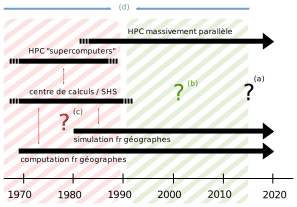
\includegraphics[width=.9\linewidth]{plan_HPC.pdf}
  \end{sidecaption}
\end{figure}


\begin{enumerate}[label=(\alph*),labelindent=\parindent,leftmargin=*]
\item Une première partie chercher à démontrer quels sont les enjeux actuels du HPC pour la géographie. Pour cet argumentaire on mobilise les textes des  géographes de l'école de Leeds, pionniers dans les usages du HPC chez les géographes \textcite{Openshaw2000b}. Ecrit dans la décennie 1990-2000, les arguments développés restent d'actualité et s'avèrent toujours très convaincants pour démontrer en quoi il est problématique encore aujourd'hui pour la géographie et les géographes de ne pas s'intéresser aux usages possibles du HPC.
\item Ce constat nous permettra d'évoquer ensuite les possibles causes à ce désintérêt actuel (zone verte), en évoquant notamment les aspects techniques difficiles du HPC, et l'enseignement informatique souvent absent des formations en géographie.
\item La troisième partie (zone rouge) questionnera les pratiques passées, en mobilisant parfois des entretien dans une démarche plus descriptive. L'objectif est de montrer qu'il y a bien eu des usages du HPC dans le passé, dans des centres de calcul en connections avec des \textit{supercomputers}, pour la computation (statistiques, analyses de données, cartographie, télédetection, etc.) mais également pour la simulation (exécution, calibrage). On découvrira également qu'il existe une filiation historique dans les usages passés et présents du HPC, car certains laboratoires mobilisent encore ce type de ressource dans certains domaines de la géographie (télédétection, simulation). Conscient de cette réalité historique, et malgré ces cas particuliers, les problématiques soulevées dans la partie (a) et (b) en ressortiront tout de même renforcé, car si ces pratiques du HPC étaient difficiles mais faisables \enquote{hier}, pourquoi se sont elles plus ou moins perdues \enquote{aujourd'hui }?
\end{enumerate}

Une synthèse sera proposée en fin de section pour faire le lien entre ces différentes sous-sections.

%\item Pourquoi cette activité a disparu ? Est ce l'absence de  challenges à la hauteur en géographie ?

%En faisant le point de façon plus détaillé sur les pratiques informatiques de certaines équipes de géographes dans les centres de calcul, nous verrons d'une part que les challenges au delà de la micro-informatique continue d'exister bien après sa démocratisation, et que des tentatives d'explorations des modèles par l'usage d'algorithmes piochés dans les outils interdisciplinaire  comme l'exploration de modèle intervient immédiatement ou presque après  des retour vers le HPC entamé depuis 2010 au laboratoire Géographie-cités des pratiques des modélisateurs de Géographie-cités une pratique resté latente jusqu'à la redécouverte  on mettra en valeur les pratiques certains des usages ayant émerger dans les années 1980 au laboratoire Géographie-cités, en explicitant
% Le point de vue d'Openshaw

\subsubsection{GéoComputation et HPC, quels enjeux pour la modélisation ? }
\label{sssec:enjeuxHPC}

Le mieux pour tenter de répondre, au moins partiellement, à cette première question, est de repartir des réflexions menées sur le HPC ces 25 dernières années par Stan Openshaw, Ian Turton et leurs collègues de l'école de Leeds. Ce qui n'était au départ qu'une intuition en 1983\Anote{openshaw_intuition} devient très vite une réalité applicative en 1986 \autocite{Openshaw1988}. Basé sur l'usage du HPC et des techniques issues de l'IA (\textit{simulated annealing},\textit{genetic algorithm}, \textit{genetic programming}), Openshaw introduit son article \textit{Building an Automated Modelling System to explore a universe of spatial interaction models} (AMS) une rupture dans la façon de construire, évaluer et de façon plus générale penser l'exploration de modèles\Anote{modele_interactionspatiale} en géographie; rupture qui fait d'ailleurs à cette période parfaitement écho aux nouveautés technologiques annoncées par les différents articles de Couclelis : Automates Cellulaires \autocite{Couclelis1985}, Intelligence Artificielle, etc. \autocite{Couclelis1986}

Le saut technologique et méthodologique permis par ce projet, ainsi que les autres projets développés en parallèle, finit probablement de persuader Openshaw et son équipe de l'étendue des possibilités bientôt offertes par l'accélération et la transformation que subit le HPC entre 1980 et 2000 (voir section suivante \ref{p:Tournant1980}).

Cette réflexion, l'école de Leeds finit en 1996 par l'intégrer dans un nouveau paradigme pour la géographie, la \foreignquote{english}{GeoComputation}

\foreignblockquote{english}[{\cite[4]{Openshaw2000b}}]{GeoComputation is not just the application of computers in geography. Nor is it just about computation for its own sake. It is meant to imply the adoption of a large-scale computationally intensive scientific paradigm as a tool for doing all manner of geographical research. Some will now claim they have been doing GC for 10 or 30 years or more. This is certainly possible, but if they were then, until 1996, it was certainly called something else; terms such as mathematical modelling, simulation, statistical modelling all spring to mind. There are three aspects which makes GC special. Firstly, there is an emphasis on the ‘geo’ subject [...] Secondly, the computation subphrase in GC is also special. It is the intensity of the computation that is especially distinctive [...] Thirdly, just as important and maybe even more significant is the underlying mindset. Computation implies a very particular paradigm based on numerical approximation rather than analytical precision. It can be based on data-driven high-performance computer-powered inductive tools rather than data free, analytically based, deductive methods. It involves trying to compute solutions to problems that could not previously be solved at all. It is based on substituting vast amounts of  computation as a substitute for missing knowledge or theory and even to augment intelligence. It could be data driven in a data mining sense, or it could be entirely data free with large-scale computer experimentation being used as a purely theoretical tool for understanding how complex systems work via modelling and simulation of their dynamics and behaviours. }

Toute une partie de la mise en oeuvre de ce paradigme est apportée par l'usage démocratisé du HPC.

\foreignblockquote{english}[{\cite[17]{Openshaw2000}}]{GeoComputation is a relatively new term invented(or first used in its current form) in 1996. It is defined as the adoption of a large-scale computationally intensive approach to the problems of doing research in all areas of geography, including many GIS applications, although the principles are more generally applicable to other social and physical sciences; [...] It involves porting current computationally intensive activities on to HPC platforms as well as the development of new computational techniques, algorithms and paradigms that can take particular advantages of HPC hardware and the increasing availability of spatial information.}

Déjà critiqué pour ses positions techniques un peu trop \enquote{innovantes}, Openshaw prend les devants en explicitant point par point dans son manifeste \textbf{ce que n'est pas} la GéoComputation.

\foreignblockquote{english}[{\cite[11]{Openshaw2000}}]{To summarize, GeoComputation is :
\begin{itemize}
\item Not another name for GIS
\item Not quantitative geography
\item Not extreme inductivism
\item Not devoid of theory
\item Not lacking of philosophy
\item Not a grab-bag set of tools
\end{itemize}}

De par son aspect paradigmatique, et l'ouverture disciplinaire qu'elle défend, cette réflexion n'est pas limitée à une application en particulier, comme en témoigne cette liste d'opportunités très génériques supportées par le HPC :

\begin{enumerate}[label=(\alph*),labelindent=\parindent,leftmargin=*]
\item \textit{To speed up existing computer-bound activities so that more extensive theory-related experimentation can be performed or to enable real-time analysis of geoinformation;}
\item \textit{To improve the quality of the results by using computing-intensive methods to reduce the number fo assumptions and remove shortcuts and simplifications forced by computational constraints that are no longer relevant;}
\item \textit{To permit larger databases to be analysed and/or to obtain better results by being able to proces finer-resolution data and make good use of very large computer memory sizes, and finally;
\item To develop new approaches and new methods based on computational technologies to provide new analytical tools and models, both of which are going to be highly important in the geoinformation-rich world of the future.}
\end{enumerate}

Comme il le précise déjà lui-même, les gains supposés ne sont pas forcément immédiats, et certains nécessitent le développement, ou le redéveloppement, de modèles ou d'algorithmes pour exploiter différents niveaux de parallélisme\Anote{dependent_application}. Dans le cadre plus restreint des modèles de simulations, nous nous intéressons principalement aux gains immédiats permis par \begin{enumerate}[label=(\alph*)]  \item la réutilisation des modèles ou algorithmes originaux libérés des contraintes techniques d'autrefois (mémoire, processeur)  \item l'utilisation d'algorithmes récents pour résoudre des problématiques autrefois insolubles \item la désimplification des modèles ou protocoles d'exploration \end{enumerate}

D'une certaine façon, la communauté des modélisateurs agents emprunte déjà dans certaines de ces pratiques des améliorations telles qu'elles sont décrites par Openshaw (a). C'est le cas par exemple lorsque \autocite{Brearcliffe2014} tente de reproduire (\textit{reproductibility} et non \textit{replicability}\Anote{reproduire_repliquer}) un des premiers modèles individu-centré développé en 1983 par Hogeweg et Hesper \autocite{Hogeweg1983}. Il est évident qu'une toute nouvelle exploration réalisée avec un micro-ordinateur d'un modèle autrefois développé sur un \textit{mainframe} doté d'un processeur à 25Mhz et 4 Mb de mémoire ne peut qu'apporter de nouveaux éclairages sur le fonctionnement du modèle. Il est en effet aisé de faire beaucoup plus d'exécution du modèle sur la même durée, et cela sans compter tous les bénéfices apportés par un tel changement de plateforme \autocite{Wilensky2007a}.

Faire le pari de la GeoComputation, c'est être plus audacieux, et ne pas seulement se contenter du HPC pour gagner du temps ou des exécutions, mais intégrer dans nos pratiques un style de pensée qui valide l'utilisation pour nos modèles de calculs difficiles ou impossibles autrement qu'en utilisant du HPC (b)(Openshaw parle de \textit{HPC-dependence} ). C'est encore dans ce cadre de liberté, en théorie illimité (il y aura toujours plus de processeurs, toujours plus puissants), que peut s'exprimer au mieux une certaine forme de créativité et d'innovation algorithmique, différente de celle plus contrainte de la micro-informatique \autocite[26-28]{Openshaw2000}. C'est le cas par exemple de la méthode \textit{Pattern Search Exploration} (PSE) développé par \textcite{Cherel2015}, qui peut nous donner une bien meilleure compréhension de la palette des dynamiques exprimables par un modèle de simulation, et cela sans avoir à le re-développer, ou à lui ajouter des objectifs à atteindre susceptibles de contraindre trop fortement cette exploration. Pour Openshaw de nombreuses connaissances sont en réalité déjà sous nos yeux, et n'attendent pour être découvertes que l'exécution de nouvelles explorations\Anote{against_oblivion}. En effet, certains modèles de simulation (modèles de Wilson ? modèles de Peter Allen ? modèle de Weidlich et Haag ? ) n'ont jamais pu être analysés dans le détail, en partie du fait de l'absence de méthodes, ou de moyens de calcul limités.

Concernant le dernier point (c), la simplification intervient déjà dans l'activité de modélisation KIDS ou KISS, via le retrait d'hypothèses inutiles, ou dans le choix du niveau d'abstraction considéré comme judicieux/suffisant vis-à-vis de la problématique donnée. En dehors du fait que la simplification soit déjà au coeur du processus général de modélisation, celle-ci est également bénéfique lorsqu'elle est motivée par une substitution, par exemple lorsqu'il s'agit de remplacer l'expression complexe d'une dynamique micro par une dynamique agrégée macro quasi équivalente (on parle de \textit{surrogate model} lorsque la substitution est par exemple motivée par un gain en performance lors de l'exécution du modèle). La simplification des explorations du modèle est plus dangereuse, car elle met en tension l'interprétation faite des résultats avec des dynamiques dont on ne connait l'expression que de façon incomplète, ou incertaine.

Un exemple récent est donné dans l'exploration du modèle de simulation LUTI MobiSim, développé depuis plusieurs années maintenant par l'équipe ThéMA. Déjà familière du mésocentre de calcul de Franche-Comté \autocite{Asch2012}, il est pourtant indiqué dans la thèse de \textcite{Hirtzel2015} soutenue en février 2015 une limite dans l'utilisation possible des infrastructures disponibles, les simulations s'exécutant seulement sur des machines de $12$ coeurs (5h30 par simulation) ou $16$ coeurs (6h30 par simulation). $8$ machines (x$12$ ou x$16$ donc) permettaient de faire des simulations en parallèle pour un total de $25$ jours de calcul, $790$ simulations exécutées équivalent à $\num{60000}$ heures de calculs cumulés pour l'analyse de sensibilité présentée. Hirtzel évoque dans sa thèse l'impact important qu'une telle contrainte a eu dans la préparation, la planification, et la simplification de cette analyse de sensibilité assez complexe devant évaluer l'interaction entre $79$ paramètres.\Anote{hirtzel}

L'effort est certes déjà impressionnant, et il ne s'agit pas ici de critiquer une expérience aussi importante techniquement et méthodologiquement pour notre discipline; toutefois, au vu de la contrainte technique régulièrement citée comme un goulot d'étranglement important pour l'exécution de ce modèle, il me semble que cela soulève une question d'accès aux ressources informatiques de ce type en SHS en général. En effet, pourquoi se contenter de cette infrastructure limitée et ne pas directement \enquote{taper à la porte} des physiciens ou des biologistes disposant d'équipements nationalisés coûtant plusieurs dizaines de millions d'euros à l'achat (20 millions d'euros pour le lot de calculateurs Ada et Turing), qui seront très probablement remplacés dans un futur proche, et cela hors coût de fonctionnement ?\Anote{naive_eject_shs}

Une autre façon de prendre conscience de l'impact possible de cette ressource dans notre quotidien de modélisateur est de prendre le problème à l'envers, comme le propose \textcite{Openshaw2000}. \foreignblockquote{english}[\cite{Openshaw2000}]{ [...] how would do you research if that PC on your desk was suddenly 10000 times faster and more powerful. It is likely that some researchers would not know what to do with it, some would not want it, but some would spot major new possibilities for using the computer power to do geography (and geo-related science) differently.}

Avec l'effacement brutal d'un grand nombre de contraintes techniques s'ouvre la possibilité d'un tout nouvel horizon de pratiques. Cette idée d'une exploration des modèles de simulation plus systématique, intervenant quasiment sans délai entre chaque remaniement conceptuel ou technique du modèle, et cela durant toute la construction, devient possible.

La possibilité d'une parallélisation à moindre coût rend également possible l'exécution et donc la confrontation de modèles de simulation en parallèle. Ce n'est plus un modèle consacrant une seule série d'hypothèses que l'on évalue, mais un ensemble d'hypothèses regroupées dans une famille de modèles dont on explore les combinaisons de façon concurrente et simultanée, fonction de la question et des données présentées. Une idée qu'avait déjà explorée Openshaw dans son générateur de modèles AMS en 1988 \autocite{Openshaw1988}, et que nous avons reprise sans le savoir à notre compte dans la progression opérée par notre équipe de modélisateurs dans GeoDiverCity \autocite{Cottineau2014b}.

Même sans avoir à réécrire nos modèles pour tirer meilleur parti d'un parallélisme potentiel et plus implicite (1 ville = 1 processeur par exemple), les gains sont déjà évidents si on se contente du niveau de parallélisme le plus courant en géographie aujourd'hui (une simulation = 1 processeur). Un modèle de simulation qui s’exécute en $5$ minutes sur $100$ villes, pourra une fois ces mécanismes validés à cette échelle, être appliqué à une toute autre échelle géographique, en $5$ heures par exemple sur les milliers de villes françaises. Sur un micro-ordinateur disposant de seulement quelques processeurs opérant en parallèle, cette \textit{scaling capacity} du modèle est inenvisageable. Par contre, sur un environnement HPC composé de milliers de processeurs, cette durée de simulation est largement compensée par le nombre de simulations réalisables en parallèle, avec cet avantage qu'une application écrite pour tirer parti de ce parallélisme d'assez haut niveau reste valide quelque soit le matériel qui l'exécute. L'achat régulier de machines supplémentaires ou le remplacement du matériel existant par du matériel plus rapide dans les parcs informatique provoque immédiatement un bond dans la durée d'exécution et le nombre de simulations qu'il est possible d'exécuter simultanément\Anote{plus_ordinateur}.

Avec la démultiplication des capacités de stockage mémoire des machines, et l'avènement de collectes de données à des échelles toujours plus fines, d'autres opportunités s'offrent au modélisateur à la fois d'un point de vue de la modélisation (la portée des axes KIDS/KISS, Stylisé/Particulier \autocite{Banos2013a} est étendue par les capacités techniques ainsi augmentées), mais aussi de la méthodologie. Il est en effet possible d'inclure dans la démarche explicative habituelle des modèles de simulation intégrant des données empiriques de résolution spatiale beaucoup plus fine qu'actuellement. La possibilité de passer d'un niveau de résolution spatiale à un autre est un moyen de ré-évaluer et de confronter la pertinence des mécanismes implémentés et des valeurs de paramètres choisies pour questionner nos connaissances théoriques supposées de la réalité, à différentes échelles d'observations.

On voit également très vite l'intérêt que peuvent avoir ces deux arguments ( \textit{scaling capacity}, résolution des données toujours plus fine) dans le cadre de la micro-simulation qui s'attache à reproduire des phénomènes observés dans des sociétés reproduites grandeur nature \autocite{Sanders2006}, souvent très difficiles à explorer du fait de temps d'exécution importants.

Des scénarios exposés ci-dessus, il faut encore ajouter cette possibilité, déjà exposée, d'utiliser d'anciens (plus rapides) ou de tout nouveaux (impossibles avant) algorithmes tirant parti eux aussi de cette parallélisation des simulations pour les explorations. On pense par exemple aux analyses de sensibilités, aux algorithmes évolutionnaires, etc.

En plus d'offrir une solution relativement pérenne, cet état d'esprit n'impose pas forcément le remplacement de pratiques de modélisation déjà existantes sur micro-ordinateur, nous verrons comment plus tard. En résumé, pour \textcite{Openshaw2000b} \foreignquote{english}{You start by tackling small and simple versions of a more complex problem and then scaling up the science as and when either the HPC systems catch-up or knowledge of algorithms, models, and theory start to show signs of being able to cope [...] \textbf{The message is smart small but think big}}

Cette façon de penser, les géographes modélisateurs en ont déjà saisi depuis quelques temps certains points, avec le développement d'une réflexion géographique appuyée par la computation, et l'adhésion à cette plus grande famille des sciences dites de la complexité. Pour ne citer que l'évolution la plus récente, le passage au paradigme informatique Agent dans les années 1990 est clairement un apport technologique externe à la géographie quantitative, appelant un renouvellement des réflexions méthodologiques et théoriques \autocite{Sanders2006} qui va bien au-delà du simple constat technique. Un apport technologique qui a redonné corps à des voies déjà explorées, tout en offrant la possibilité de résoudre des problèmes techniques ou conceptuels autrefois insolubles en les abordant sous un nouveau jour (le paradigme objet/agent est - entre autre - bien plus flexible pour la représentation des interactions entre entités). Certes la révolution HPC d'après 1990 n'entre pas (encore) en ligne de compte, mais l'idée d'un dépassement par l'apport technologique est déjà là.

L'accession successive à de nouvelles technologies a toujours servi à développer un projet scientifique qui se nourrit de cette multiplicité d'approches. Il faut y voir un processus d'accumulation, et non pas une succession poussée par une mode ou une autre.

Si l'on prend l'exemple de la théorie évolutive des villes de Denise Pumain \autocite{Pumain1997}, force est de constater que pratiquement toutes les nouveautés, technologiques et/ou paradigmatiques susceptibles d'un apport théorique ou méthodologique servant cette théorie (et par extension les objets géographiques concernés), ont été mises en perspective de façon critique dans chaque publication : les outils statistiques unis et multi-variés, les analyses factorielles, les systèmes dynamiques non linéaires, les réseaux de neurones, les automates cellulaires, la modélisation agent, tout a été testé avant d'être intégré dans la boîte des outils potentiellement remobilisables. Car il n'y a pas une technique meilleure qu'une autre, mais bien une combinatoire de techniques constitutives d'un raisonnement scientifique, dans laquelle chacune peut exposer tour à tour de multiples facettes \autocite{Sanders2000, Mathian2014}.

Il n'est pas interdit donc de penser que les progrès de l'informatique, si l'on cherche bien, apportent toujours au modélisateur de son époque les moyens de devenir un meilleur aventurier, pour reprendre l'image de l'explorateur donné par \textcite[22]{Banos2013} ou encore en citant la vision \textcite[1]{Openshaw2000b} \foreignquote{english}{Computation permits the investigator to test theory by simulation, to create new theory by experimentation, to obtain a view of the previously invisible, to explore the previously unexplorable, and to model the previously unmodellable.}

En un sens, cette seule phrase me semble suffisante pour imager tous les espoirs que nous avons placés dans ces usages renouvelés du HPC pour l'exploration des modèles de simulations en géographie.

Pour \textcite{Openshaw2000}, tous ces nouveaux usages ont acquis une forme de matérialité dès que la démocratisation du HPC s'est enclenchée. Il suffisait déjà dans les années 2000 de quelques efforts pour saisir cette chance. C'est d'ailleurs tout l'enjeu de \textcite{Turton1998} à cette période, lorsqu'ils proposent, forts d'une expérience enracinée dans les années 1980 et de multiples prototypes fonctionnels innovants, de former les géographes aux usages simplifiés du HPC en moins de 200 pages. Presque 15 ans plus tard, et en dehors du colloque annuel de \textit{GeoComputation}, pourquoi cet argumentaire, pourtant brillant, développé par les supporters de la \textit{GeoComputation}, n'a pas été entendu et mis en pratique outre-Atlantique ?

%Pour de multiples raisons, dont certaines déjà évoqués par Openshaw en 2000 - et sur lesquels nous reviendrons indirectement en étudiant le cas francais - il semble malheureusement que ces appels soient restés vains en dehors du cercle des géographes de Leeds, et des participants majoritairement anglo-saxon (plus géomaticiens ? plus géographes ?) régulièrement présent à la conférence \enquote{GeoComputation}.


\subsubsection{Quelles explications possibles pour ce désintérêt envers le HPC après 1990 ? }
\label{sssec:desertionHPC}

\textcite[20-22]{Openshaw2000} citent un certain nombre de critères qui peuvent selon eux expliquer ce retard chez les Anglo-saxons.

\begin{enumerate}[label=(\alph*),labelindent=\parindent,leftmargin=*]
\item Jusqu’à récemment (1998 du point de vue de l’auteur), cette ressource n’était pas satisfaisante pour envisager une utilisation plus généralisée en géographie. Il est à noter selon lui que la plupart des usages du HPC en géographie ne permet pas un usage incrémental, et il existe un véritable seuil à partir duquel les ressources à disposition deviennent intéressantes. Il est vrai que la mémoire mise à disposition des géographes dans ce type de machine est par exemple un facteur important d’utilisabilité, car que cela soit pour l’analyse spatiale ou la simulation, il est important de pouvoir utiliser et stocker un maillage spatial suffisamment représentatif de la situation étudiée.
\item  La critique de fond adressée aux quantitativistes en géographie depuis les désillusions des années 1970, et la montée en puissance de géographie(s) plus qualitatives.
\item L’absence de tradition dans l’utilisation de ressources de calculs importantes, et le peu d’applications sont en partie la conséquence des deux points suivants.
\item  Les objections philosophiques héritées des critiques du néo-positivisme ou positivisme logique, et la peur de ne pas arriver à concevoir l’outil technologique comme un support neutre : \foreigntextquote{english}[{\cite[21]{Openshaw2000}}]{Computation is just a tool, and how the tool is used and what it is used for and the context in which it is used depend on the interests, skills, and value systems of the user, which are themselves grounded in contemporary society.}
\item La complexité \enquote{apparente} de la programmation et la nécessité d'acquisition de nouvelles capacités qualifiées de difficiles par beaucoup de géographes ne programmant plus depuis longtemps.
\item Le fait qu’on puisse imaginer cette activité computationnelle comme un renoncement automatique à toute pensée critique.
\item Il n’y a aucun agenda de recherche et aucune ressource informatique mise à disposition des géographes pour s’initier à l’usage des HPC.

\end{enumerate}

L'histoire et le contexte anglo-saxon sont évidemment très différents du contexte français, mais les points évoqués ici par Openshaw forment toutefois une première liste à minima de pistes à explorer depuis notre position actuelle. Les limitations techniques (a), et le peu de projets (c) ont pu être un facteur limitatif évident jusqu'à la fin des années 1990, mais aujourd'hui ces arguments sont plus difficiles à mobiliser. C'est également le cas du dernier point (g): des appels à projets et des infrastructures sans précédent sont en train d'émerger ces dernières années à un niveau européen, la motivation des géographes pour intégrer ce type de projet devrait logiquement être beaucoup plus audible. Restent donc les critiques classiques (b)(d)(f) dont on s'apercevra par la suite qu'elles continuent d'être mobilisées pour freiner le retour pourtant nécessaire d'un débat sur les rapports de la géographie à l'informatique, un frein visible aussi dans les enseignements de cette discipline (e).

Pour comprendre de quelles limitations techniques il s'agit, il faut faire le point sur ce qu'implique cette transformation touchant le HPC dans les années 1990. Une fois mise en perspective toute la difficulté pour un géographe d'accéder seul à ce type de ressources, il faudra bien se poser la question plus générale de l'autonomie que l'on veut donner aux géographes sur le plan des enseignements informatiques, avant d'imaginer dans la continuité de nos pratiques, une solution plus concrète.

\paragraph{Tournant des années 1990 dans le HPC}
\label{p:Tournant1980}

La plupart des informations historiques et techniques proposées ici sont tirées des ouvrages suivants \autocites{Fox1994, Fox1988, Seitz1985, CM2-1990, Lerman1993, Padua2011, Dietrich1984}[81-84]{Culler1998, Steele2011} ainsi que des \textit{Working Report} suivant \autocites{Athas1987, Su1987, Seitz1983, Seitz1984a, Seitz1984b} dont la liste plus complète est disponible sur le \href{http://authors.library.caltech.edu/view/person-az/Seitz-C-L.html}{@site} des archives de Caltech.

Entre les années 1960-1980 on peut encore parler d'une phase de recherche et d'expérimentations, avec la création et l'amélioration des premiers \textit{supercomputers} à processeurs vectoriels, particulièrement adaptés au calcul scientifique rattaché généralement à cette époque à l'architecture SIMD\Anote{simd_def} qui va ensuite dominer le marché du HPC jusqu'en 1990\Anote{liste_hpc_simd}. Sur la base de ces premiers super ordinateurs, très coûteux, des années pré-1980, le domaine naissant du HPC va ensuite connaître un certain nombre de révolutions entre 1980 et 1990.

%Sur une autre branche, les MIMD, de nombreuses expérimentations concernant les architectures multi-processeurs, et la gestion du parallélisme ont également lieu : D825 (1962), CDC 6500 (1966), Multics system (1969)

Entre autres innovations technologiques, l'introduction progressive des microprocesseurs depuis les années 1970 va permettre d'aller beaucoup plus loin dans l'invention fin 1970, début des années 1980 de nouveaux paradigmes de construction pour les ordinateurs. %Le parallèlisme peut être pensé autrement, et s'appuyé sur la baisse des couts qui frappe l'industrie informatique dans les années 1980.

Danny Hillis publie dès 1981 un mémo au MIT donnant les concepts \autocite{Hillis1981} d'une nouvelle machine massivement parallèle nommée \textit{Connection Machine} (CM), qui va amener un certain renouveau dans la façon de penser ce type d'architecture SIMD.

Ce dernier travaille d'abord avec Minsky et Papert au laboratoire MIT sur le langage LOGO, avant de créer la société \textit{Thinking Machine} en 1983. Celle-ci commercialise une série de CM (\textit{Connection Machine}) d’architecture SIMD (puis MIMD\Anote{mimd_def}), dont le premier prototype est présenté à la DARPA en 1985, et la première livraison commerciale est réalisée en 1986. Ces machines constituent une référence historique initiale importante dans la construction de machines composées de plusieurs milliers de processeurs.

Sachant que David Hillis s'est largement inspiré des travaux de Minsky et de son livre \textit{Society of Mind}\Anote{mind_minsky}, cette architecture n'est pas sans évoquer l'image idéalisée du fonctionnement d'un cerveau\Anote{note_cm} tel qu'on se la représente à l'époque en IA symbolique, les CM's ciblant d'ailleurs résolument ce type d'application avec l'implémentation machine d'une version spécialisée de lisp, le *lisp (star lisp). Ainsi même si ce type d’architecture SIMD (dominante sur le marché des HPC jusqu’aux années 1990) est généralement plus complexe à appréhender, la CM a par exemple été utilisée très tôt pour développer des applications rattachées aux systèmes complexes dans le cadre de l’\textit{Artificial Life} et des \textit{Complex Adaptative System} (CAS), car elle s’appuie dans sa construction (voir la participation de Feynamn, et de Wolfram sur l'architecture de la CM) sur la propriété de parallélismes propres aux automates cellulaires (1 processeur = 1 cellule/patch)\Anote{CA_physical}. Les CM proposent certes une alternative intéressante par cette possibilité augmentée de parallélismes, mais elles brillent aussi par leur performance, la CM-1 (prototype) de 1985-1986 , la CM-2 (commercialisation) de 1986-1987 (2.5 à 6 GFlops), la CM-5 (qui passe d'une architecture SIMD à MIMD, avec 1024 processeurs) est numéro 1 du premier \href{http://www.top500.org/featured/systems/cm-5-los-alamos-national-lab/}{@Top500} de 1993 avec 59.7 GFlops sur le Linpack test. En comparaison, à l'IDRIS en 1993, le Cray C98 Axis avec 8 processeurs dépasse à peine les 7 GFlops.

Des travaux similaires ont également lieu depuis les années 1970 dans l’équipe de physiciens de Tommaso Toffoli (en contact aussi avec les travaux du français Yves Pomeau \autocites{Toffoli2005,Toffoli1987}) au MIT, qui finissent par concevoir, dans le courant des années 1980, un \textit{hardware} spécifique (CAM-6, CAM-8) pour paralléliser les CA en s’appuyant sur leurs propriétés fondamentales \autocite{Toffoli1987}\Anote{ca_simd_avantage}.

%Epez1993

En France, il existe également des développements similaires en physique, avec la famille de machines R.A.P (Réseau d’Automates Programmables) démarrée à l'ENS en 1986 à Paris, OUPPI (Ordinateur Utilisant des Processeurs Parallèles Intégrés) à Marseille \autocites{Manneville1989, Hiebeler1990}. Ces deux architectures différentes (voir \autocite{Hillis1981}) inspirées par les CA \autocites{Hillis1984, Hillis1989, Toffoli1987} et issues de travaux démarrés au MIT, sont également utilisés pour des applications scientifiques similaires \autocite{Toffoli2005}. L’équipe de l’UCLA de David Jefferson et ses modélisations de fourmilières (\textit{Tracker}, \textit{Genesys}, \textit{AntFarm}) utilisent une CM contenant pour la première fois plusieurs milliers de fourmis, un préalable pour observer des comportements auto-organisationnels. Ou encore la première version parallélisée du langage LOGO qui sera développé sur ce type de machine CM avant de passer plus tard sur Macintosh (Starlogo 1991). Au Los Alamos National Lab (LANL), Langton recrute Hiebeler\Anote{hiebeler_parcours} en 1989 pour travailler sur le logiciel \textit{CellSim} initié en 1988 et mis à jour jusqu’en 1990. Hiebeler possède une expertise sur les CAM-6, mais également sur les CM car il a travaillé à \textit{Thinking Machine} entre 1991 et 1992, ce qui lui permet de développer une interface sur ce logiciel vers des machines de type CM. Ces deux types de \textit{hardware} seront voués à un échec commercial, pour des raisons diverses qui ne touchent pas forcément au seul aspect scientifique, car ces outils ont constitué de réelles avancées d’un point de vue de la computation scientifique aux moments où ils étaient disponibles.

Dans l'avalanche d'innovations ayant lieu dans le courant des années 1970-80 au niveau du \textit{software} et du \textit{hardware} (topologie hypercube, vlsi et microprocesseur, baisse des coûts de production, langage acteur \autocite{Hewitt1973}, Unix, etc. ), le paradigme de construction basé sur l'architecture MIMD\Anote{exemple_simd_mimd} connaît lui aussi un certain rafraîchissement au tout début des années 1980, bien avant la livraison de la première Connection Machine CM-1.

C'est le cas par exemple du prototype \textit{Caltech Cosmic Cube} dont la première version fonctionnelle est finalisée en 1983\Anote{caltech}. Ce dernier est une architecture MIMD à mémoire distribuée, et s'appuie sur une gestion logicielle pour l'envoi des messages entre processeurs. Plusieurs logiciels et plusieurs versions de cette machine vont être commercialisés\Anote{caltech_logiciel}. Évidemment incompatibles entre eux, cette variété de matériels et de logiciels préfigure l'expression chez les utilisateurs d'un besoin rapide pour la constitution d'un standard/norme d'échange de messages implantés de façon transparente sur chaque machine : la norme \textit{Message Passing Interface} (MPI), dont on parle plus ensuite. Cette machine universitaire plusieurs fois améliorée de façon interne au laboratoire de recherche (Mark II (1984)/ Mark III (1986)) agrège autour d'elle plusieurs dizaines de programmes de recherches en tous genres, pour son utilisation ou son amélioration. Cette machine va également être déclinée dans des versions commerciales plus ou moins différentes (meilleurs processeurs, mémoire augmentée, ajout de composants pour réaliser des traitements spécifiques, utilisation d'Ethernet pour les échanges de messages, nombre de noeuds constitutifs, logiciels pour la gestion des messages différents, etc.) : nCUBE, Ametek, Intel iPSC, FPS T-Series, Paralex Gemini.

Autre avantage de cette machine, pour 1\% du prix du Cray-1, elle produit 10\% de ses performance, ce qui prouve pour la première fois la faisabilité et les bons résultats d'une architecture parallèle utilisant des composants standards à moindre coûts. L'intel 8086 étant le premier micro-processeur de la famille x86 que l'on va retrouver dans une variante sur les IBM PC vendus dès 1981 à plusieurs millions d'exemplaires. %Sur la base d'une architecture MIMD à mémoire distribué la communication entre processeurs se fait sur la base d'une topologie en hypercube, avec un protocole d'échange de messages entre processeurs qui n'est plus piloté de façon physique par des routeurs, largement inspiré par la logique acteur de Hewitt.

On pourrait également citer par exemple les travaux sur le NYU Ultracomputer, de David E. Shaw sur la machine \enquote{Non-Von} (pour \enquote{Non Von Neumann}) de la Colombia University, le \textit{Goodyear Massively Parallel Processor} (MPP), et probablement d'autres, moins connus. Toujours est-il que ces différentes initiatives sont toutes reconnues au début des années 1980 comme étant des pionnières dans la construction d’architectures \textbf{massivement parallèles}, c'est-à-dire mettant en oeuvre au moins plusieurs centaines de processeurs.

C'est avec l'apparition ou la maturation durant les années 1980-1992 d'une véritable grappe de nouvelles technologies qu'émerge la notion moderne de \textit{cluster} : apparition des protocoles d'échanges de messages PVM puis MPI, mais également création d'Ethernet, développement d'Internet,  miniaturisation constante et augmentation des fréquences d'horloges des processeurs, apparition de logiciels et de matériels libres, etc. Ainsi cet esprit de réutilisation de \enquote{matériel standard} déjà expérimenté par l'équipe de Berkeley sur le \textit{Cosmic Cube} trouve son apogée dans l'invention plus ou moins simultanée de projets de mise en grappes de micro-ordinateurs dans les années 1990, en s'appuyant non plus cette fois-ci sur une architecture (\textit{hardware}) spécialisée reliant les différents composants (processeurs), mais sur leur simple mise en réseau appuyée par des applications (\textit{software}) de partage et d'échange de données efficients entre les machines.

%Cluster p292 / le projet NOW de Berkeley (NOW emphasized high-end workstations, high performance networks, and proprietary software) / et le projet Beowulf de la Nasa (Beowulf emphasized low cost personal computers, mass market networks (Ethernet), and the new trend in open source software including the Gnu editors and compilers and the Linux operating system)

Mais en dehors de ces applications et de ces architectures pionnières, d’un point de vue utilisateur la révolution tient surtout de l’émergence, et de la mise à disposition d’un plus large public, de protocoles de communication permettant de s’abstraire complètement de l’infrastructure qui supporte physiquement le parallélisme, que celui-ci opère sur un \textit{cluster}, ou sur des ordinateurs distants reliés par Internet, ou un mélange des deux. Ce type de norme a ainsi permis le développement plus aisé de programmes distribués de façon massivement parallèle, sans avoir à se soucier du langage à adopter, et de l’ensemble des contraintes techniques propres à chacune des technologies supportant ce parallélisme. Par exemple, la norme MPI (\textit{Message Passing Interface}) est devenue depuis sa création en 1992-1994 le modèle quasi-dominant implémenté (encore aujourd’hui) sur l’ensemble du matériel dédié à une utilisation partagée.

Ainsi, ces différentes visions d'une infrastructure support du parallélisme peuvent cohabiter et soulager l'utilisateur de la contrainte liée au \textit{hardware}. Il est possible aujourd'hui de programmer un logiciel qui marche tout à la fois sur son propre \textit{cluster} personnel construit à base d'Arduino/Raspberry/Edison, que sur des architectures techniques plus complexes mélangeant différentes technologies ou paradigmes choisis pour une utilisation adéquate. Ainsi, les supercalculateurs d'aujourd'hui sont souvent eux-mêmes des formes de \textit{clusters}, à la fois héritiers des premiers prototypes expérimentant des combinaisons de \textit{hardwares} et \textit{softwares} innovants, mais également héritiers de toutes les avancées liées à la démocratisation qui touchent l'ensemble des aspects matériels et logiciels dans l'informatique.

Le calculateur Turing de l'IDRIS\Anote{idris} est construit selon une architecture massivement parallèle (MPP de type \textit{MIMD distributed memory} \autocite{Snir2011}) cumulant de très nombreux noeuds de calcul ($\num{6144}$ noeuds de $16$ coeurs à $1$ Go de mémoire par coeur) pouvant être connectés selon de multiples topologies. Celui-ci peut être accédé comme une seule et même machine (jusqu'à $\num{65536}$ coeurs simultanés autorisés en exécution). En comparaison, le \textit{cluster} ADA dispose d'une mise en réseau locale très rapide de plusieurs centaines de noeuds de calculs séparés : $332$ noeuds d'architecture type \textit{Symmetric MultiProcessor} SMP) qui mélange deux types d'architectures : \textit{MIMD shared memory} sur le SMP et \textit{MIMD distributed memory} pour assurer la communication entre les SMP. Chaque noeud dispose d'un ensemble de processeurs multi-coeurs ($32$ coeurs) avec une mémoire partagée plus importante ($4$ à $8$ Go par coeur), ce qui fait de ce calculateur ADA une architecture multi-processeurs destinée à des calculs plus communs (jusqu'à $\num{2048}$ coeurs autorisés en exploitation), tout en restant très facilement extensible via l'ajout de nouveaux noeuds.

Comme on peut le voir dans les quelques paragraphes ci-dessus, le jargon technique (SIMD, MIMD-SH, MIMD-DM, DMM, SMP, etc.) qui accompagne l'environnement du HPC est un préalable à l'utilisation probablement rédhibitoire pour qui s'intéresse au HPC sans être du domaine.

\medskip

\textbf{Mais, a-t-on besoin de tous ces détails techniques et de ce jargon ?}

\medskip
Comme le disent si bien \textcite{Openshaw2000} : \foreignquote{english}{We really do not need a whole lot of unnecessary details from computer science and computer engineering. Why not simply take it for granted and concentrate on using the technology? [...] Geographers should be viewing parallel computing as a tool that can be used on their problems; there is absolutely no need to know more than about 0.01 percent of the technical details of how the hardware actually works}

Ce qui nous amène à l'utilisation de ces différents types de ressources groupées sous le terme très générique d'HPC. Pour ce qui est des ressources pilotées par GENCI, toutes les demandes passent par un dossier administratif indiquant la nature du projet scientifique et la demande d'attribution d'heures correspondantes. Les projets doivent être déposés plusieurs mois à l'avance, avant d'être approuvés par un conseil scientifique réuni une à deux fois par an \autocite{GENCI2015}. Sur le \href{https://www.edari.fr/}{@site} de Demande d'Attribution de Ressources Informatiques (DARI) qui accueille les dépôts de dossier GENCI, on trouve la liste des 11 comités d'évaluation existant en 2015, et comme on peut le constater, il n'y a tout simplement pas de comité réservé pour les sciences humaines et sociales : environnement, écoulements non réactifs, écoulements réactifs ou/et multiphasiques, biologie et santé, astronomie et géophysique, physique théorique et physique des plasmas, informatique algorithmique et mathématique, dynamique moléculaire appliquée à la biologie, chimie quantique et modélisation moléculaire, physique chimie et propriétés des matériaux, nouvelles applications et applications transversales du calcul.

Là encore, nous sommes très éloignés des pratiques, mais également des besoins pour la modélisation en SHS. Si on regarde à l'inverse du côté des sciences physiques, ce type d'accès est tout à fait normalisé, l'attribution du temps de calcul faisant souvent partie intégrante du projet de recherche déposé par les étudiants. Il existe aussi des encadrements dédiés pour les scientifiques ou les étudiants voulant apprendre à manipuler ces ressources. La \enquote{Maison de la Simulation} dispose par exemple pour les travaux pratiques de ses formations d'un accès dédié aux ressources HPC disponibles sur le campus du plateau de Saclay. C'est le cas aussi de l'IDRIS qui met à disposition des usagers du CNRS des formations dédiées.\Anote{formation_idris}

Si on regarde du côté des services offerts par un autre type de ressources HPC, les grilles de calculs (\textit{Grid Computing}) offrent une flexibilité d'emploi qui s'avère en revanche très intéressante, et cela malgré des limites évidentes pour certains usages.
% A reintegrer.
Elles offrent le plus haut niveau de parallélisme envisageable, et permettent de partager des exécutions de calculs sur des ressources complètement hétérogènes distribuées n'importe où sur la planète, en communiquant avec elles via Internet. Cette ressource ne fournit pas de mémoire partagée et/ou de mécanisme de partage de données entre les différents noeuds, considérés comme autonomes, ce qui limite leurs utilisations dans le cadre de certaines applications nécessitant à la fois beaucoup de mémoire partagé, une communication forte entre les différents noeuds de calculs, et/ou un niveau de parallélisme interne au programme : c'est le cas par exemple des astrophysiciens travaillant sur des modèles de simulation de l'univers composés de plusieurs milliards d'étoiles en interaction.

Il existe effectivement différents niveaux de granularité envisageables quand on parle de paralléliser des applications :
\begin{itemize}[label=\textbullet]
\item le parallélisme peut être envisagé de façon interne au niveau des primitives : des traitements opérants habituellement de façon séquentielle sur les objets contenus dans une liste vont être parallélisés sur l'appel d'une primitive dédié.
\item le parallélisme peut être envisagé toujours de façon interne au programme, mais au niveau des objets cette fois-ci : c'est le cas par exemple d'une simulation multi-agents où les agents s'exécutent sur un environnement distribué.
\item le parallélisme peut être externe au programme : si on reprend l'exemple d'une simulation, alors ce niveau de parallélisme permet l'exécution simultanée de plusieurs simulations, en s'appuyant par exemple sur un environnement de calcul distribué.
\end{itemize}

Les niveaux ne sont pas exclusifs, et une application peut très bien cumuler ces différents niveaux. Toutefois le parallélisme le plus simple et le plus immédiatement disponible consiste pour le modélisateur à attribuer un noeud de calcul par simulation, car il n'y a théoriquement aucune modification à apporter au programme. Dans ce cas-là, il s'agit d'un niveau de parallélisme externe au programme.

De multiples équipements informatiques implantés et accessibles à des mailles géographiques différentes, d'utilisation pour la production ou la recherche, sont réunis et accessibles aux chercheurs par le biais de divers portails administratifs. Appelées Organisation Virtuelle (\textit{Virtual Organization}), ces entités administratives virtuelles régissent l'attribution des ressources de la grille de calcul en fonction des différents accords passés entre les acteurs intervenant dans la constitution de la grille. Divers critères rentrent en jeu dans ce découpage, ceux-ci peuvent être de nature thématique, technique,selon des zones géographiques, politique, etc.

En France,depuis 2010 c'est le GIS France-Grilles (vo.france-grille.fr) qui mène cette mission de mutualisation entre les différents acteurs publics (Laboratoires, Méso-Centres, Centres nationaux) et privés au niveau national (Initiative Nationale de Grille ou NGI), mais aussi européens en étant le partenaire et représentant francais de l'EGI (European Grid Infrastructure). Piloté par des institutions scientifiques majeures (MESR, CNRS, CEA, INRA, INRIA, INSERM, CPU, RENATER), ce Groupe d'Intérêt Scientifique (GIS) coordonne la mise en place d'une grille de calcul nationale a priori accessible à toutes les disciplines scientifiques par le biais de différentes VO. D'après les statistiques 2012, sur $700$ utilisateurs regroupés en $89$ VO rattachées à la VO France-Grilles, seulement $12$ utilisateurs sont enregistrés dans la catégorie systèmes complexes, et $0$ pour les sciences sociales. Sur $\num{1450}$ référencements entre 2010 et 2013, la collection HAL maintenue par France-Grilles pointant les publications utilisateurs de cette grille nationale, il y avait une seule publication référencée en sciences de l'homme et de la société. Aujourd'hui il y a environ une dizaine de publications référencées, provenant en majorité de géographes.

Dans le cadre des SHS en France, il y a également la mise à disposition de ressources informatique de ce type, notamment par la collaboration au CNRS entre le \href{http://cc.in2p3.fr/}{@CC-IN2P3} et l'ancien TGE Adonis devenu TGIR \href{http://www.huma-num.fr/}{@Huma-Num}. Human-Num offre une liste de services à disposition des laboratoires, dans lequel figure un accès à des ressources informatiques de type grille de calcul, traitées par le biais de l'IN2P3, et accessibles via la technologie \textit{Grid-Engine}.

Pour utiliser tout ou partie de ce type de ressources HPC, il faut que le laboratoire d'accueil soit rattaché à une de ces entités administratives virtuelles, qui pourra ensuite délivrer un certificat d'accès unique au futur utilisateur (fichier crypté contenant une clef unique personnalisée reconnue par les machines de la grille), renouvelable tous les ans. Le laboratoire doit être enregistré auprès de l'autorité de certification du CNRS GRID2-FR pour pouvoir récupérer et valider des certificats. La ressource est ensuite disponible de façon illimitée et relativement immédiate dès lors qu'on possède l'un de ces certificats. La ressource rattachée à chaque VO est généralement partagée avec l'ensemble des différents utilisateurs de celle-ci, même s'il peut exister dans certains cas des systèmes de quota. Une fois inscrit dans une VO, le laboratoire désigne une personne de confiance capable de signer et de délivrer des certificats de façon locale au laboratoire. Le processus pour délivrer les certificats est complexe, mais reste en définitive beaucoup simple qu'un dépôt de dossier administratif et scientifique ensuite jugé par un conseil scientifique thématique, comme c'est le cas via GENCI \autocites{GENCI2014,GENCI2015}. Intégrée par une seule personne, la procédure paraît d'un point de vue utilisateur moins coûteuse (pas de dépôt de dossier scientifique), et très simple (la demande d'attribution et la réception du certificat se font directement par Internet).

Ces modalités d'accès sont donc beaucoup plus intéressantes du point de vue d'un modélisateur dont l'activité de construction nécessite d'évaluer très régulièrement ses modèles de simulation par l'usage de techniques diverses, toutes relativement exigentes sur les aspects computationnels : analyse de sensibilité, plan d'expérience divers, usage d'algorithmes d'optimisation pour la calibration ou l'exploration des comportements du modèle, etc.

En résumé, nous nous intéresserons principalement par la suite aux \textbf{grilles de calculs}, car :

\begin{enumerate}[label=(\alph*),labelindent=\parindent,leftmargin=*]
\item La finesse de parallélisme engagée dans cette architecture est largement suffisante pour engager une première étape dans la voie du HPC immédiatement bénéfique pour la simulation en géographie,
\item On a accès à une ressource globale masquant l'hétérogénéité du parc de machines qu'elle représente, ce qui en fait potentiellement une ressource en constante évolution/amélioration
\item Les modalités d'accès à cette ressource sont plus compatibles avec les pratiques réelles des modélisateurs
\end{enumerate}

Mais il y a un hic dans tout cela. Si l'émergence, l'amélioration successive, et le maintien ces 20 dernières années de la norme MPI comme un standard indétrônable dans l'industrie du HPC a certes beaucoup simplifié les prérequis nécessaires pour user de ces ressources, le 0.01\% d'Openshaw censé représenter le seuil minimal d'informations techniques qu'un débutant devrait avoir à apprendre pour manier ce type de ressource HPC inclut forcément des bases en informatique. Il faut en effet pouvoir comprendre et utiliser les fonctions MPI implémentées dans un langage de programmation, quelqu'il soit.

Des formations à la programmation, à l'architecture technique spécifique du HPC, sont évidemment ouvertes dans ces différents instituts (GENCI, IDRIS, Maison de la Simulation, etc.). Seulement ces organisations ne sont pas connues de la plupart des géographes, et le niveau technique nécessaire à la compréhension de ces formations est bien trop complexe et trop éloigné du domaine de compétence des géographes pour que ceux-ci s'y présentent spontanément.

Autrement dit, et sans cette formation, une fois l'utilisateur connecté à une ressource HPC, quelle que soit sa forme, que se passe-t-il lorsque le curseur du terminal informatique clignote dans le vide? Quels sont ensuite les manipulations, les commandes, les fonctions à connaître, à appeler, à intégrer dans nos programmes pour exécuter nos calculs, nos simulations en parallèle sur ces infrastructures ?

Même dans le cadre d'une mise à disposition pour les SHS, la ressource est fournie sous sa forme la plus brute\Anote{human_num_note}. On imagine qu'il y a peu de monde disposant, sans projet ou structure interdisciplinaire associée, du niveau suffisant pour mettre en oeuvre l'amorce technique nécessaire à la bonne utilisation de cette ressource informatique.

En définitive, et malgré des efforts conséquents des géographes de l'école de Leeds \autocite{Openshaw2000} pour introduire le HPC et la norme MPI aux géographes dans les années 1990-2000, on ne peut pas vraiment dire que cette pratique se soit diffusée outre-Manche ces 15 dernières années (et peut-être même en dehors d'un cercle très restreint des géographes informaticiens de Leeds).

Faut-il donc persévérer dans cette voie, ou existe-t-il aujourd'hui des solutions alternatives pour amener le HPC jusqu'au bout des doigts des géographes modélisateurs ?


%\item Des logiciels permettent de s'abstraire de la couche de programmation MPI normalement nécessaire pour accéder à ce type de ressources HPC,

%https://hal.archives-ouvertes.fr/FRANCE-GRILLES
%https://hal.archives-ouvertes.fr/FRANCE-GRILLES/search/index/q/%2A/domain_t/shs/
%GRID2-FR

%MPP p574

%Distributed Memory = Chaque processeur a sa mémoire propre, et peux accéder à la mémoire des autres via une forme de connection (réseau local, réseau spécialisé, bus spécifique, etc.)

%Blue Gene L = Distributed Memory MIMD computer

\paragraph{Quelle place pour les débats sur la place de la \enquote{pensée informatique} dans la géographie ?}
\label{p:Tournantenseignements}

Comme le disait déjà Michel Serres en 2011 dans sa séance d'introduction aux nouveaux défis de l'éducation \enquote{Avant d’enseigner quoi que ce soit à qui que ce soit, au moins faut-il le connaître. Qui se présente, aujourd’hui, à l’école, au collège, au lycée, à l’université ?} \autocite{Serres2011} A tous ceux qui pensent la programmation comme un apprentissage hors de portée de nos étudiants en licence, il faut leur ouvrir les yeux sur ce nouveau monde, celui bien réel décrit par Michel Serres dans \enquote{Petite Poucette} \autocite{Serres2012}, celui des étudiants qui se présentent aujourd'hui dans nos enseignements, et sur les initiatives de ceux qui ont déjà compris qu'apprendre à programmer était une activité aujourd'hui accessible dès le plus jeune âge.

Si l'on prend l'exemple d'autres pays, comme aux États-Unis en 2013, lorsque le président Obama prend la parole pour la \textit{Computer Science Education Week} organisée par la fondation \href{http://code.org}{@code.org} créee la même année : \foreignquote{english}{If we want America to stay on the cutting edge, we need young Americans to master the tools and technology that will change the way we do just about everything.} Si l'on peut regretter que cette initiative soit portée essentiellement par les fonds de grandes sociétés informatiques américaines, force est de reconnaître que l'intention politique est bel et bien là. D'autant plus que ce type d'initiative est loin d'être isolé, aux États-Unis, mais également sur la scène internationale. En France un réseau gagnant peu à peu le territoire est en train d'émerger, dans différents lieux d'accueil (bibliothèques, musées, FabLab, réseau des cantines numériques, écoles d'informatiques, clubs, etc.), des regroupements d'initiative locale, ou nationale.

Par exemple, l'initiative \href{http://Simplon.co}{@Simplon.co} \Anote{simplon} créée par \textcite{Bardeau2014} (le livre est conçu comme un manifeste pour \enquote{Lire, Ecrire, Compter, Coder}), est une entreprise au format juridique original (modèle ESS hybride : une entreprise solidaire d’utilité sociale agréée et une association d’intérêt général) qui propose des formations intensives de 6 mois pour les moins de 25 ans, sur dossier, quelque soit leur parcours scolaire. Récemment reconnue et soutenue par le gouvernement comme d'intérêt général, cette initiative, en train d'essaimer un peu partout en France, n'est qu'une parmi des centaines d'autres initiatives aux origines, aux formes différentes, mais aux objectifs communs : \enquote{La programmation pour tous}. Ce même groupe tient par exemple un annuaire \autocite{Simplon2015} qui compte aujourd'hui plus de 42 ressources différentes (club, réseau, écoles, sites, événements, etc.) à destination de l'apprentissage de la programmation chez les plus jeunes, et ce n'est évidemment qu'un échantillon.

Autre exemple, l'initiative des enseignants néozélandais de \textit{Computational Science Unplugged}, qui donne corps au principe universel de \enquote{pensée informatique} (\textit{Computational Thinking}) au travers d'un livre d'activités illustré, pensé pour être utilisé par tout le monde, déjà traduit\Anote{traduction_unplugged} en plusieurs langues\Anote{texte_csunplugged}.

En France, il aura fallu l'émergence spontanée et de plus en plus évidente d'un réseau d'initiatives citoyennes, la pression d'une communauté internationale bien plus au fait de ce mouvement, et l'échec répété de plusieurs projets nationaux, pour qu'en 2012-2013 soient \textbf{ enfin consolidées des instances (Conseil National Numérique) et une politique nationale à ce sujet}.

Les lignes énoncées par l'Académie des Sciences en 2013 \enquote{L’enseignement de l’informatique en France. Il est urgent de ne plus attendre} \autocite{AScience2013}, ou encore les différents rapports du récent Conseil National du Numérique (dont le dernier Jules Ferry 3.0) \autocite{CNNum2014}, les soutiens solides entre ces acteurs\Anote{appui_academie_science}, les lettres ouvertes répétées des associations comme la Société Informatique de France \href{http://www.societe-informatique-de-france.fr/lettre-ouverte-a-monsieur-francois-hollande-president-de-la-republique-concernant-lenseignement-de-linformatique/lettre-ouverte-a-monsieur-francois-hollande-president-de-la-republique-concernant-lenseignement-de-linformatique-2/}{@SIF}, soutenues et relayées par l'association quadragénaire spécialiste de ces questions \textcite{EPI2014}, \textbf{tous ces écrits sont unanimes, il faut agir au plus vite pour dispenser un véritable enseignement informatique, et former ainsi des citoyens qui seront acteurs du monde numérique}.

La réforme en cours pour le collège a annoncé très récemment (\autocite{SIF2015} 18 mai 2015) des pistes concrètes qui rejoignent les lignes énoncées\Anote{extrait_CNN} par le Conseil National du Numérique dans son dernier rapport \autocite{CNNum2014}. Reste à voir quels moyens effectifs seront alloués pour mettre en place et pérenniser véritablement ces annonces :
\begin{itemize}[label=\textbullet]
\item une initiative au codage dès le primaire,
\item la programmation informatique au collège,
\item une nouvelle option informatique en seconde et en première.
\end{itemize}

Un projet dont il faut espérer qu'il ne sera pas abandonné au prochain mandat, car ce n'est pas la première fois que de telles annonces jalonnent l'histoire assez chaotique des relations entre l'éducation, l'informatique et les politiques\Anote{historique_EPI}.

\medskip

\textbf{Quid de l'université et des sciences sociales dans ce mouvement ?}

\medskip

Pour le moment, il est triste de voir que les initiatives prises dans l'enseignement supérieur de la recherche, comme celle de \enquote{France Université Numérique}, ne traitent cette révolution que sous l'angle unique des \textit{Massive Open Online Course} (MOOC) et d'un usage finalement très partiel et passif des technologies au service de l'éducation. L'avenir nous dira donc si cette prise de conscience finira par toucher un système universitaire, pour le moment absent dans ce débat.

Il existe déjà des filières spécialisées dans l'enseignement cumulé des mathématiques et de l'informatique pour les Sciences Humaines et Sociales (MIASHS), offrant des parcours interdisciplinaires intéressants. Mais ce que nous disent aujourd'hui ces différents rapports et cette multitude d'initiatives citoyennes, c'est qu'il est tout à fait possible d'enseigner l'informatique et sa logique sans faire appel à un support mathématique, ou même à un langage informatique en particulier\Anote{simple_bloc}, des outils qui peuvent intervenir bien plus tard dans la formation.

On observe également depuis quelques années déjà l'émergence de la thématique \textit{Digital Humanities} dans les débats sur l'informatique et les SHS. Ce mouvement\Anote{definition_complexe} qui se fait avant tout l'écho d'une relation renouvelée des SHS au regard des évolutions touchant l'informatique\Anote{humanite_digitale_histoire}, se retrouve aussi dans des structures fédératives où sont plus ou moins mises en valeur certaines composantes de ce mouvement. Le TGIR Huma-Num par exemple fait avant tout ressortir un projet dont les termes\Anote{huma_num} paraissent assez éloignés des problématiques de programmation, de simulation, ou même tout simplement de calcul, alors même qu'il existe dans le giron de cette infrastructure des utilisateurs potentiels ou déjà actés de ce type de ressource : ALPAGE \autocite{Costa2012}, EQUIPEX MATRICE, GeoDiverCity, etc.

En effet même si cette ressource HPC est bien retenue dans la grille de services proposés par le TGIR, elle semble d'une part très peu valorisée dans les formations et les guides pratiques proposés par la structure, et d'autre part largement insuffisants pour des applications réelles, par exemple en simulation en géographie\Anote{human_num_notecout}.

Mais tout cela concerne la partie recherche d'un mouvement où l'heure en est encore au manifeste et à la réflexion, dont on trouve extraits dans : les discussions de la version française des \textit{Humanities and Technology Camp} \href{http://tcp.hypotheses.org/}{@ThatCAMP} et leur manifeste \autocite{THATCamp2010}, les livres comme celui de \textcite{Deuff2014} ou du collectif rassemblé autour de \textcite{Mounier2012}, le numéro 2 de la nouvelle revue électronique transdisciplinaire \href{http://rsl.revues.org/355}{@RSL}, le rapport commandé par l'Institut français \autocite{Dacos2015}, etc.

Il est donc encore assez difficile de voir quels impacts ce mouvement a sur l'enseignement. On trouve toutefois une tentative pour le THATCamp2012 de \href{http://pireh.univ-paris1.fr/DHfrancophone/index.php?rem&val=g%C3%A9ographie}{@cartographie} des enseignements en humanités numériques sur la France \autocites{Berra2012b,Clavaud2012}, régulièrement mise à jour, et où semble-t-il aucune formation en géographie n'apparait. S'agit-il d'un retard de notre discipline dans l'intérêt qu'elle porte à ce type de mouvement, ou plutôt d'un effet de catégorisation lié au cloisonnement disciplinaire francais, la question amène probablement un débat qui dépasse de loin cette introduction. Parmi les rares acteurs de la géographie ayant pris conscience des enjeux scientifiques se cachant derrière cette première ouverture disciplinaire, on trouve une intervention de Thierry Joliveau à la conférence plennière du THATCamp de Lyon en 2014 \href{http://dhlyon.hypotheses.org/587}{@Video}).

Ces quelques pistes n'offrent qu'une entrée très limitée dans un débat méritant un travail de recherche plus conséquent, qui reste encore à faire. Il est difficile en effet de trouver une réflexion globale et actuelle interrogeant les rapports existants entre l'informatique et la géomatique, l'informatique et la géographie, la géomatique et la géographie, au niveau de la recherche et des enseignements, mais aussi dans la place que ces débats sont amenés à jouer dans celui plus large des humanités numériques.

%Quelle projection peut on faire au delà d'une utilisation passive du SIG, ou de la simple utilisation de logiciels de statistiques, une vision \enquote{utilitariste} de l'informatique dont on a vu qu'elle serait amené à changer.

Déjà cité comme étant un des rares géographes/géomaticiens étant intervenu dans les \textit{THATCamp}, Thierry Joliveau fait aussi partie de ces quelques scientifiques à même aujourd'hui de questionner l'actualité des relations entre géographie et géomatique. Dans le volume 5 de son HDR on trouve ainsi une section \enquote{Géomatique et géographie, débats et enjeux} qui ouvre une première réflexion sur ce sujet en 2004.

Dans son argumentaire, Joliveau n'hésite pas à s'appuyer sur le malaise et les querelles importantes soulevées par le SIG chez les Anglo-saxons dans les années 1990 \autocite[472-473]{Joliveau2004}. La lecture presque en parallèle des écrits d'Openshaw montre bien l'extension prise par ce débat entre informatique et géographie, loin d'être finie au tournant des années 2000. En effet, dans leur manifeste pour le HPC \autocite[2]{Openshaw2000}, paru la même année que l'ouvrage sur la GéoComputation \autocite{Openshaw2000b},  Openshaw et Turton n’hésitent pas à engager les géographes dans une métaphore qui les met en proie à une forme de maladie des plus virulentes. S'en prenant plus spécifiquement aux géographes \enquote{SIG-istes} (et accessoirement aux sciences sociales en général), c’est une forme particulièrement menaçante de \foreignquote{english}{let others do the programming for us} qui condamnerait peu à peu ces scientifiques à délaisser la programmation plutôt qu’à s’en emparer pour devenir acteurs de leurs propres outils\Anote{openshaw_virus}. Dans la continuité de sa guerre engagée contre les technophobes, Openshaw s'attaque  maintenant à une forme plus perverse de ce mouvement, celui-ci fustigeant l'immobilisme technologique et l'idée qu'on puisse penser l'outil et son utilisation comme une fin en soi. En se démocratisant, les outils deviennent d'une façon ou d'une autre bornés par les questions qu'ils permettent d'aborder. Il faut toutefois sortir de ce qui peut apparaître comme une fatalité pour l'étudiant, en lui donnant les moyens d'inventer seuls, ou avec de l'aide, ses propres solutions à ces nouvelles questions.

Bien que le contexte dans lequel le débat se pose initialement, et la forme prise en réponse aux critiques soit au final assez différente de l'autre côté de l'Atlantique, il semble bien qu'il y ait un socle commun à la base de cette prose critique questionnant les usages du SIG en géographie.

\blockquote[{\cite[474]{Joliveau2004}}]{Le débat dans la géographie anglo-saxonne traduit la réaction méfiante d'une partie de la communauté géographique par rapport à cette technoscience triomphante. C'est une réaction du même ordre qui a conduit les géomaticiens français issus de la géographie comme de l'informatique à veiller à se placer en dehors de cette vague de la géomatique \enquote{industrielle et commerciale} et à travailler en amont, sur des questions et des concepts, des méthodes ou des outils non pris en compte dans les produits logiciels du marché.}

Une méfiance, voire une prise de recul nécessaire, qui ne constitue pas en soi un problème, à condition toutefois de ne pas déroger à l'exercice nécessaire et légitime d'un questionnement scientifique sur le statut des connaissances ainsi produites par ce qui serait une nouvelle \enquote{ingénierie géographique}.

Sur ce point le débat reste ouvert, et \textcite[474-477]{Joliveau2004} nous renvoie vers une lecture plus approfondie des positionnements épistémologiques empruntés par une GIScience anglo-saxonne, qui s'est depuis armée d'un discours en réponse à une \enquote{[...] tradition explicative de la géographie savante [...]} qui en général \enquote{[...] ne se satisfait pas d'un programme perçu comme essentiellement descriptif et principalement technique. La tradition critique de la géographie y voit même un projet dangereux}.

Concernant ce socle commun, \textcite[477]{Joliveau2004} nous dit que \enquote{Les critiques des SIG du débat anglo-saxon auront sans doute rappelé d'autres débats plus anciens. P. George était parti en 1972 à l'assaut de \enquote{l'illusion quantitative en géographie} (George 1972). Il est frappant de constater que nombre de ses arguments correspondent point par point à ceux des critiques actuels des SIG. [...] 30 ans plus tard, certains continuent à s'inquiéter d'une dérive technique de la géographie à cause des SIG (voir plus loin).} L'auteur fait référence notamment aux velléités édulcorées (par rapport aux critiques anglo-saxonnes) et peu renseignées de \autocite{Staszak2001}. Mais pour Joliveau ce n'est pas tant le débat que l'absence de débat qui pose problème en France. La menace d'une dérive technologique sous-entendue par ces auteurs prend alors, au grand plaisir de ces derniers, des atours de prophétie auto réalisatrice\Anote{joliveau_texte}. Des auteurs dont Joliveau\Anote{joliveau_pgeorge} et Openshaw sont, il me semble, tous deux bien d'accord pour dire à propos de leurs discours que ceux qui s'y accrochent encore n'y connaissent en définitive absolument rien, et ne méritent donc aucun crédit.

%Alors même que la place du SIG fait parfois encore débats pour ce qui est de sa place dans l'enseignement - même si la situation s'est déjà grandement amélioré si on en croit Joliveau sur son blog en 2009 -, devrait on en plus se préparer à être totalement exclus de la majorité des futurs projets necessitant l’usage du HPC, c'est-à-dire de la programmation pour le HPC, en géographie ? Sans aucun doute, comme on l'a déjà remarqué au tout début de cette introduction.

Les enjeux semblent importants, et le débat passionnant. Presque 10 années plus tard, qu'en est-il de cet état de la question et de la place du SIG en géographie dans la recherche et l'enseignement ?

Au vu de la rapidité d'évolution des techniques, et de la démocratisation massive qu'a connu le SIG dans de multiples disciplines ces dernières années, il serait aventureux de se lancer dans une quelconque projection de cet état de fait datant de 2004, en 2015. On pourra par contre toujours se référer aux écrits pertinents de Joliveau et continuer ainsi à prendre le pouls d'un débat intervenant à la frontière du monde professionnel et universitaire, entre la géographie et géomatique, tel que développé sur son blog \href{https://mondegeonumerique.wordpress.com/}{@Monde-GeoNumérique}.

Il est intéressant par contre de prolonger les critiques énoncées en les transposant dans ce parti pris souhaité par Openshaw, celui d'un saut technologique supplémentaire, au-delà du SIG et même de la programmation, dans la maîtrise de la programmation spécifique au HPC. Car si ces critiques interviennent encore de façon dommageable dans l'intégration du SIG comme outil standard à disposition des géographes, alors il n'est pas difficile d'extrapoler, et de se dire qu'elles le sont probablement tout autant pour la programmation, et pour le HPC.

A ce stade, est-il possible d'envisager, comme Openshaw en fait déjà état en 2000 pour les Anglo-saxons, un retard dans l'adoption du HPC en géographie en France ? Doit-on reprendre à notre compte ces craintes d'une géographie dépassée, en retard, oubliée, déjà avancées par plusieurs géographes dans le passé\Anote{joliveau_peur} ?

Ne prend-on pas le risque de passer à côté de thématiques comme le \textit{Big-Data}, les \textit{Smart-Cities}, qui engagent derrière cette couverture marketing des financements importants amenant la possibilité de traiter et d’analyser des données géographiques récoltées à des échelles et avec des moyens inégalés jusque là ? Alors même que l’Europe est passée très près de débourser plus d'un milliard d’euros sur le projet FuturICT intégrant une très forte composante simulation, la programmation pour la modélisation est loin d’être couramment enseignée chez les géographes et les chercheurs géographes. Quant à l'introduction aux moyens et aux techniques du HPC, elle est quasi-inexistante, voire utopique. Doit-on s’attendre à voir ces précieuses données géographiques analysées comme de simples données \enquote{xy}, au détriment des géographes français et aux profits de seules sociétés privées, surfant sur la vague des financements, et avec qui il faudra ensuite peut-être négocier pour accéder à ces données ?

%; c'est donc sans étonnement qu'on apprend les désagrement qu'a connu Openshaw avec les critiques dès la présentation de son prototype AMS.

En ce sens, l'urgence pointée par Joliveau de repenser le rapport de la géographie à l'informatique dans l'enseignement\Anote{formation_informatique} est essentielle pour le futur de la discipline, mais celle-ci dépasse de loin il me semble la seule question du SIG. Il ne s'agit pas simplement pour l'université de donner un débouché professionnel aux géographes en leur apprenant à programmer dans des master spécialisés - ce qui est un début, c'est vrai -, mais de leur donner de façon plus générale, comme on pu le faire pour les statistiques en leur temps, les bases suffisantes pour qu'ils puissent comprendre et améliorer les outils développés par les géographes dans le passé\Anote{aquoicelasert}, établir des collaborations actives et non plus passives avec les autres disciplines déjà rompues à l'informatique, mais aussi produire des outils de recherche en accord avec les développements de la société actuelle.

La plupart des auteurs abordant ce débat semblent d'accord, l'apprentissage de la programmation que cela soit pour la modélisation chez les géographes \autocite[64]{Banos2013}, dans les réflexions de géomaticiens \autocite{Joliveau2004}, dans les récits des géographes modélisateurs \autocites{LeBerre1987, Cuyala2014}, en histoire dans l'enseignement \autocite{Genet1993}, ou encore dans le cadre plus large des humanités numériques\Anote{code_humanite}, dans le cadre des initiatives citoyennes, ou depuis peu dans les institutions, \textbf{l'apprentissage de la programmation n'est pas une fin en soi, elle est un moyen pour une fin} \autocite[67]{Deuff2014}. Elle est ce socle de connaissance initial, dont le contenu reste encore à définir, qui permet d'engager cette co-construction autour de l'informatique entre les disciplines.

L'accès à la programmation, ou du moins à la \enquote{pensée informatique} pour tous, dans les filières universitaires, et plus spécifiquement en géographie (en dehors des seuls master spécialisés), est un projet qui est, semble-t-il, encore à construire.

%Tout comme Netlogo a su ces dernières années fédérer les modélisateurs, ce mouvement doit être de nouveau capturé dans la création d’un outil accueillant ces échanges pour ce qu’ils sont, c’est à dire bilatéraux (et non pas l’expression d’une commande), imparfait (car manipulant des concepts au sens différents, voire conflictuel), et imprégnés (il n’est pas facile d’adopter un nouvel angle d’analyse). L’objet de cette co-construction ne se concentre plus uniquement sur le modèle, mais sur l’exploration de celui-ci, et cela en utilisant tout la réunion des moyens humains et informatique faisant déjà usage du HPC.


%http://web.media.mit.edu/~mres/papers/designing-for-tinkerability.pdf

%Nous verrons par la suite que la solution proposé basé sur l'utilisation du logiciel OpenMOLE réduit encore un peu plus ces efforts, et vient s'accoler au plus pret des usages actuel chez les géographes modélisateurs.

% Seconde question

%\hl{transition transition transition}

Si le HPC est un acronyme à la définition relative, il doit être étudié \textit{in situ} pour mettre face à face challenges scientifiques et moyens computationnels au moment où ils sont disponibles.

%On a bien vu dans le chapitre 1 que les géographes, et certains modélisateurs pionniers dans les sciences humaines, s'étaient déjà tournés vers ce qui était alors les rares et uniques ressources informatiques permettant d'être en adéquation avec les enjeux scientifiques en ces temps. Cette motivation, il me semble que les géographes l'ont trouvé déjà une première fois en françe dans les années 1970, dans l'application notamment de toute nouvelles techniques pour la statistiques ou la simulation, les deux marchant de paire avec la découverte de l'informatique.

%Nous verrons dans la section \ref{sssec:centre_habite} que ces traces existent, même si elles sont encore assez peu documentées.

Repris de façon hétérogène par les sciences humaines, l’usage de \textit{supercomputers} est resté pendant quelques décennies le premier contact \enquote{contraint et forcé} que ces pionniers ont eu avec l'informatique. A ce titre, le chapitre 1 a déjà donné un aperçu des nombreux travaux réalisés par ces chercheurs en sciences humaines, et il me semble important de re-souligner le courage qu'il a fallu pour braver à plusieurs, ou parfois seul, toutes les contraintes à la fois intellectuelles, financières et physiques permettant d'approcher de telles machines, avant tout construites pour les besoins des sciences physico-mathématiques.

En résumé, on pourrait donc arguer qu'il s'agissait \enquote{d'un autre temps}, et que le \textit{supercomputer} était alors le seul moyen de faire de l'informatique. Oui, c'est vrai, mais en partie seulement.

Pour mieux comprendre dans quel contexte nous nous situons à cette époque, il faut tenter d'imaginer un monde quasi-dénué de toutes perspectives informatiques impliquant une utilisation autonome de l'ordinateur\Anote{gibson}. Difficile alors d'évoquer cette rupture conceptuelle et physique qu'a pu être l'arrivée de la micro-informatique dans certaines pratiques bien installées des sciences humaines. Tout d'un coup un objet un peu plus gros qu'une calculette apparait sur votre bureau, et permet de réaliser des calculs quasi-similaires à ce que vous faisiez en à peine quelques heures de plus sur des \textit{supercomputers}.

Considérée comme un événement bénéfique par quelques scientifiques déjà convertis à cette pratique de l'informatique depuis 10 ans, ou objet considéré comme inutile, décoratif, voire dangereux pour beaucoup; force est de constater que l'implantation progressive des \textit{micro-computer} dans les facultés au cours des années 1980 a quand même fini par rendre en partie obsolète une pratique de l’informatique jusqu'alors contrainte à l'utilisation des centres de calcul.

Toutefois, il ne faudrait pas se contenter ici de dérouler un argument trop commode, selon lequel dès lors que la micro-informatique apparaît, tous les géographes disparaissent des centres de calcul fréquentés auparavant.

Si la majorité des géographes vont effectivement se tourner vers la micro-informatique dès lors qu'elle se démocratise, on retrouve aussi dans plusieurs équipes des accointances plus ou moins durables avec certains centres de calcul, accointances dont on trouve encore trace physique aujourd'hui dans des politiques d'équipement, mais aussi dans la fréquentation ou la construction de structures d'accueil scientifique.

Pourtant, si l'on applique de façon rétroactive l'argument d'Openshaw faisant du challenge scientifique une nécessité motivant l'usage du HPC, alors il nous faut aller plus loin que ce simple constat et montrer en quoi l'apparition et la démocratisation des micro-ordinateurs n'a pas été un événement suffisamment convaincant pour que certaines équipes décident de continuer à pratiquer ces centres dans le courant des années 1980-1990.

Une entrée même partielle dans cet historique des pratiques - tel qu'on s'y essaye par la suite dans la section \ref{sssec:histo_centrecalcul} - permet, à défaut de produire une étude exhaustive, d'apporter quelques éclairages sur cette question.

Devant les difficultés d'usages des moyens informatiques de l'époque, la \enquote{mise en oeuvre} même de l'informatique apparaît en elle-même comme un défi nécessitant co-construction. Celle-ci se fait au croisement des formations de certains universitaires à la programmation, et de la fréquentation de creusets interdisciplinaires dans, et/ou autour des centres de calcul, que cela soit en SHS, ou chez les géographes (Strasbourg, Besançon, Montpellier, Paris). Il nous faut rappeler qu'à cette époque, il est impossible d'utiliser un programme de statistiques ou de cartographie sans avoir recours à des notions de FORTRAN.

Cette diversité des pratiques, des collaborations, est donc la preuve qu'il y avait dans la pratique de ces centres interdisciplinaires d'autres projets, d'autres challenges plus stimulants que celui du seul accès à une ressource informatique pour faire des statistiques. Car à y regarder de plus près, l'autonomie et l'indépendance permises par l'utilisation du micro-ordinateur, sont des qualités qui peuvent à l'inverse être aussi approchées comme une invitation au repli sur soi, à la dispersion des efforts impliquant l'apparition de \enquote{re-création informatique} stérile\Anote{remarque_informaticien_roue}, et l'effacement possible de ce riche horizon interdisciplinaire et de l'activité de co-construction qu'il supporte \autocite{Banos2013}.

En un sens il n'y a donc aucune raison pour que certaines de ces interactions interdisciplinaires, une fois nouées, ne disparaissent toutes subitement avec l'apparition de nouveaux logiciels ou de nouveaux équipements. Il est impossible de donner un point de vue global sur ce point, et nous verrons, comme l'a déjà noté \autocite[372]{Cuyala2014}, que les premiers géographes formés à la programmation informatique adoptent vis-à-vis de celle-ci, et par rapport à l'enseignement ou à leur recherche, des postures personnelles ou collectives tout à fait diverses. La seule chose que l'on peut avancer de façon plus certaine, c'est qu'il y a bien eu un jour la disparition des enseignements de programmation d'une partie des cursus de géographie quantitative, au profit de l'utilisation d'outils.

En résumé, le \textit{supercomputer} a continué à exister et à être accessible tant qu'il y a eu de la place pour les SHS dans les centres de calcul. Certains géographes ont donc continué à l'utiliser, d'autres non, pour diverses raisons dont on donnera un aperçu par la suite.

% Voir si le paragraphe ne meriterait pas d'etre plus haut

Concernant le cas plus spécifique de la simulation, nous pourrons d'ailleurs revenir plus précisément dans la section \ref{sssec:contexte_modelisateur} sur une série de collaborations entre géographes et physiciens/chimistes qui illustre ce que Denise Pumain décrit aussi comme l'assurance \enquote{de se donner des instruments à la hauteur des questions que l'on se pose}, preuve supplémentaire que les défis scientifiques s'inventent aussi dans l'importation et l'adaptation de techniques et de méthodologies issues d'autres disciplines.

%Une matrice de 9 par 9 ou de 73 par 73, telle qu'elle est utilisée par exemple par Openshaw dans son générateur de modèle AMS \autocite[40]{Openshaw1988}, est intéressante d'un point de vue théorique, mais ne permet pas une montée en complexité suffisante permettant la comparaison avec l'empirie. Comme l'avait déjà souligné Openshaw, ce n'est qu'une fois enclenchée la transformation du HPC au milieu des années 1980 que certaines applications peuvent enfin dépasser le stade de prototype. On évoque dans la section \ref{sssec:Tournant1980} abordant plus en détail les changements opérant à cette période les difficultés d'usages par exemple des automates cellulaires sur de large grille.

%N'est on pas dans une situation similaire ou la construction et l'exploration de nos modèles de simulation est encore largement contrainte par les ordinateurs équipants nos postes de travails, et cela probablement pour encore quelques temps ?

% Rejoignant le constat du chapitre 1, cela prouve aussi que les sciences humaines et les géographes ont été capables d'apprendre l'informatique et de surmonter des obstacles bien plus importants que ceux pouvant se dresser devant nous aujourd'hui pour accéder au HPC (ce qui explique aussi le manuel d'Openshaw sur le HPC \autocite{Openshaw2000}, qui croyait vraiment à cette possibilité de dépassement dans la discipline), preuve que lorsque les enjeux scientifiques sont à la hauteur, rien n'est impossible.

\subsubsection{Un bref historique des usages du HPC en géographie et en Sciences Humaines et Sociales}
\label{sssec:histo_centrecalcul}

%Avant de revenir sur cette question, il est important de noter que ces centres de calcul, à la différence peut être de ce qu’ils sont devenus pour certains ces dernières années, sont avant tout des lieux propices à l’inter-disciplinarité dans les années 1970-1980.

% SMA encore existant ?
% PACTE : Sonia Chardonnel, Elise Beck

En 1984, à l'occasion du Congrès International de Géographie se tenant pour la première fois à Paris, \textcite{Faugieres1984} cite dans l'ouvrage de synthèse \textit{La recherche géographique Française} une enquête du CNRS datée de 1982\Anote{bulettin_intergeo}. Il en tire les éléments suivants : sur $162$ formations en géographie ou dirigées par des géographes, $31$ seulement ont pu fournir des indications sur l'utilisation de moyens informatiques, $8$ départements de géographie n'ayant aucune activité informatique. Sur ces $31$, l'utilisation se répartit de la façon suivante, $9$ utilisent des centres de calcul, $12$ ont à leur disposition des terminaux, $2$ ont accès à des \enquote{mini}, et $13$ ont acquis un ou plusieurs micro-ordinateurs ($23$ dans l'ensemble des départements).

En 1983, \textcite[367]{Lecarpentier1983} expose dans les \textit{Annales de Géographie} une première description technique du \textit{micro-ordinateur} et de ses avantages, en partie pour contrebalancer un usage de l'ordinateur en géographie qui selon lui \enquote{ [...] reste donc marginale en regard des énormes possibilités offertes. En ignorant cet outil-là, après bien autres, la géographie laisse le champ libre à d'autres disciplines plus réceptives à l'évolution des mentalités et des techniques. Souhaitons que ce numéro spécial des \textit{Annales de Géographie} soit l'occasion - et le signe - d'un renversement de tendance et passons en revue la tâche immense qui attend le géographe, s'il veut bien apprendre à utiliser l'ordinateur et notamment le micro-ordinateur autrement que de façon marginale et accessoire.}

Il commente également (p 348) les résultats d'une enquête à laquelle il a eu accès pour fonder son analyse, sans donner les chiffres, mais qui tend à vérifier les conclusions données précédemment par Faugières\Anote{bulettin_intergeo_a}) : \blockquote{ Une enquête récente menée auprès de géographes universitaires français a montré que le recours aux centres de calcul reste le moyen le plus répandu mais que l'utilisation du mini- ou du micro-ordinateur en est souvent complémentaire. Les grandes universités (Paris, Montpellier,  Grenoble, Strasbourg) utilisent surtout ou exclusivement leur centre de calcul et apparaissent sous-équipées en matériels spécifiques. Les micro-ordinateurs se diffusent rapidement un peu partout mais leur généralisation est gênée par l'absence de logiciels adaptés aux besoins des géographes. Quelques équipes (Besançon, Lille, Rouen) ont entrepris la réalisation de logiciels de ce genre [...] Finalement, malgré sa diffusion rapide dans de nombreux secteurs d'activités, le micro-ordinateur reste un outil mystérieux et inconnu pour la plupart des géographes.}

Cette période des années 1980 reste d'approche assez délicate, car si les centres de calcul semblent rester un pôle d'accroche important pour de nombreux géographes, elle est aussi marquée par l’émergence à la fois externe de nombreux \textit{packages} logiciels développés par une nouvelle industrie florissante du logiciel informatique, ou interne, par les développements de géographes devenus pour certains experts en programmation informatique. Pour \autocites[444]{Joliveau2004}{Waniez2010}, la diffusion de la micro-informatique et de logiciels plus évolués sur le plan graphique et de l’interaction homme-machine courant des années 1980 a ainsi rendu complétement obsolète la fréquentation des centres de calcul pour l’usage statistique et cartographique. \textit{Quid alors des autres usages ?}

Pour appuyer les discussions sur cette époque, quelques témoignages ont pu être collectés durant le premier semestre 2015. Je remercie d'ailleurs par avance la géographe et professeure Colette Cauvin, le sociologue et professeur Philippe Cibois, l'historien et professeur Jean-Philippe Genet, l'ingénieur de recherche au CNRS Alexandre Kych, la géographe et professeur Denise Pumain, et la directrice de recherche Lena Sanders pour les informations qu'ils ont bien voulues me transmettre sur ces pratiques pionnières de l'informatique dans les SHS, et plus spécifiquement sur les usages des centres de calcul alors à leur disposition. Si l'apparition de non-géographes dans cette liste peut apparaître comme étrange en premier abord, ces témoignages seront aussi l'occasion de mettre en avant les autres \enquote{fonctions} supportées par ces lieux, qui reviennent souvent dans les entretiens comme les creusets d'une pratique solidaire et/ou interdisciplinaire de l'informatique. Les extraits qui viennent sont pour certains tirés de témoignages et d'échanges dont on trouve une reproduction intégrale en annexe \ref{chap:entretiens} de la thèse.

L'apprentissage de la programmation FORTRAN et la maîtrise d'un contexte matériel complexe daté des années 1970 est un passage quasi-obligé pour la plupart des géographes français voulant appliquer les techniques quantitatives. Cette aprentissage apparaît nécessaire pour exécuter les programmes informatiques \enquote{révolutionnaires} venus des Etat-Unis \autocite[150,127]{Cuyala2014}, mais également pour exécuter les nouvelles statistiques unies et multivariées, quand ce n’est pas tout simplement pour maîtriser à minima les entrées / sorties d’un superordinateur. Information difficile à trouver sans réaliser un travail historiographique important, la thèse de \textcite{Cuyala2014} nous donne quand même quelques informations sur le bagage techniques de certains des premiers géographes quantitativistes francais : Sylvie Rimbert (formation au Fortran à Ottawa p 137) ;  Cosinschi, Racine, Lemay, Cavalier (formation Fortran à Ottawa p 150), Pumain ( Montréal p 153), Marchand (p 154), Durand-Dastès (p 313) Dumolard (p 323), et sûrement d’autres du fait de leur origine québecoise, de leur profil hybride, ou de leur attirance pour une certaine rigueur mathématique (p 157-158).

Pour introduire les usages de l'informatique et des centres de calcul chez les géographes dans les années 1970-1990, on fait appel à une typologie en trois classes introduite par \textcites{Wieber1980}[448]{Joliveau2004} : l’accès aux packages logiciels ou à la programmation directe en cartographie et en statistiques se fait soit en interne lorsque les équipes ou les universités possèdent du matériel, soit par un accès direct aux centres de calcul, soit par un accès indirect par des terminaux en contact avec ces mêmes centres. Si la présence de centres à proximité des équipes coïncident souvent, la qualité de l'activité ne saurait se rapporter à cette seule présence ou à la taille d'une université.

L'innovation à Besançon tient par exemple de cette première catégorie. \textcite[131]{Cuyala2014} souligne l’importance des collaborations entre Jean-Claude Wieber, géographe alors issu de l’institut de géographie alpine sous le patronage éclairé de Paul Claval, et le mathématicien Jean-Philippe Massonie.

%IBM 1630 ?
\textcite{Massonie1986} a créé le laboratoire Mathématique Informatique et Statistiques (MIS) en 1964. Implanté dans une UER de Lettres et Sciences Humaines à l’université de Franche-Comté de Besançon, ce laboratoire atypique accueille une inter-disciplinarité qui n'est pas seulement dirigée vers la géographie\Anote{massonie_texte}. Disposant d’un petit centre de calcul rattaché à l'UER, la présence initiale d'un matériel modeste (IBM 1130 jusqu'en 1975 \autocite[22]{Wieber1980}, puis IRIS 50, IRIS 80 plus puissant \autocite{Massonie1986}) n'empêche en rien l'innovation. Cette équipe partie des premières à user des toutes nouvelles méthodes statistiques \autocite{Massonie1971}, mais c'est également elle qui va impulser l'important colloque interdisciplinaire de Besançon à partir de 1972. Intitulé \enquote{L'application des méthodes mathématiques à la géographie}, ce lieu d'échange joue selon \autocite[331]{Cuyala2014} un poids indéniable dans l'histoire de la géographie quantitative française; on trouvera pour plus d'informations un compte-rendu des dix ans d'activités dans les Annales de Géographie en 1983 \autocite{Massonie1983}, deux ans avant la disparition du colloque.

Avant même le début des années 1980, ce groupe investira très vite dans du matériel micro-informatique, en partie du fait de nouvelles contraintes liées à l'utilisation du matériel, comme le laisse deviner le commentaire de Massonie sur sa page Internet personnelle à propos de l'IRIS \enquote{Cela devient un vrai ordinateur parce qu'on y a plus accès. La bête est enfermée dans une cage de verre, des techniciens le font marcher. Le matin on dépose ses cartes dans un bac, à midi on récupère les cartes et le listing des résultats. On a perdu le côté ludique. Les informaticiens ont pris le pouvoir. Certes il est plus rapide, mais que m'importe que mon calcul qui durait 1 heure, ne dure plus que 10 minutes, si je ne récupère les résultats que 3 heures après.} Un micro-ordinateur est acquis par Massonie dès 1978 pour développer \enquote{un logiciel d'analyse des données dont l'utilisation soit bon marché et accessible à des non-informaticiens.} Devant les performances satisfaisantes de ces micro-ordinateurs, et l'autonomie qu'ils permettent, de nombreux logiciels micro sont adaptés ou créés à partir de là (ANACONDA, SADE, PATATE, etc.)\Anote{massonie_1978} \autocite{Massonie1986}. Cette volonté d'une \enquote{informatique conviviale} \autocite{TSH1984}, on la retrouve par la suite tout au long des transformations successives englobant ou accompagnant cette structure initiale originale.

Ce laboratoire a été le support dans la décennie 1980 d'un secteur de recherche (AMMSIOSHE) groupant plusieurs laboratoires (Géographie, Histoire, Littérature, Philosophie, etc.), mais également d'un GIS \enquote{Techniques nouvelles en sciences de l'homme} et d'un DEA pluridisciplinaire \enquote{Méthodes et Techniques nouvelles en sciences de l'Homme et de la Société} \autocite{TSH1984}. Le laboratoire MIS deviendra en 1997 le MTI SHS (Méthodologie et Technologies de l'Information appliquées aux Sciences de l'Homme et de la Société) \autocite{Girardot2004} et regroupera dans son projet l'ambition d'être à la fois une plateforme technologique, un lieu d'interdisciplinarité pour les sciences de l'homme et de la société, et un partenaire pilote dans la formation à l'innovation mêlant informatique et sciences humaines (ISTI). Après le départ à la retraite de Jean-Philippe Massonie, ce projet interdisciplinaire construit sur 30 ans se poursuit également avec l'émergence d'un nouveau projet scientifique autour de la MSHE C. N. Ledoux (2002), structure commune aux deux universités de cette région \autocites{Favory2003, Favory2009}. Le MTI SHS est aujourd'hui intégré comme équipe de recherche technologique (ERT) pour l'intelligence territoriale au sein de l'UMR multi-site ThéMA créée en 1999, qui participe également dans certains pôles de la MSH de Dijon et de la MSHE Ledoux de Besançon. Cette MSHE sert une optique mutualiste, avec la mise à disposition des autres disciplines de services humains et matériels appartenant initialement à ThéMA. La structure de la MSHE Ledoux dispose en effet en 2015 de ses propres calculateurs de taille moyenne (PowerEdge R815, Dell Précision 7500) destinés aux traitements locaux de données lourdes, preuve aussi que cette \enquote{culture du centre de calcul} reste une condition importante dans la marche d'un environnement interdisciplinaire. Une remarque aussi à mettre en perspective du tout centralisé, et de l'absence d'équipements similaires dans d'autres MSH en sciences humaines. Il existe également un partenariat entre ce laboratoire et le mésocentre (centre de calcul régional) de Franche-Comté \autocite{Asch2012}, sur lequel par exemple tournent la plupart des simulations du modèle LUTI Mobisim.\autocites{Thema2010, Hirtzel2015}

Le pôle strasbourgeois impulsé par Sylvie Rimbert regroupe à partir de 1968-1969 Etienne Dalmasso, Monique Schaub, Colette Cauvin\Anote{informations_colette_cauvin}. En 1970, le géographe ayant acquis de solide compétence en statistique et en informatique Michel Pruvot intègre l'équipe à son retour du Canada, également complété en 1971-72 par Gérard Schaub, puis Henry Reymond en 1973 \autocite[135-153]{Cuyala2014}. De retour du Canada, ce dernier remplace Etienne Dalmasso alors nommé à Paris. L'équipe active en statistique informatique est principalement composée de Michel Pruvot, Colette Cauvin, Sylvie Rimbert et Henri Reymond. %@bla

Fort d'une formation à l'étranger pour certains, apprentissage initié ou complété par les formations du CNRS (1971 à Strasbourg, 1972 à Paris) pour d'autres, ce petit groupe est en tout cas très rapidement opérationnel en informatique, en statistique et en cartographie, dès le début des années 1970. C'est cette triple compétence qui permet à l'équipe d'utiliser au mieux et très rapidement les ressources informatiques à leur disposition sur le campus universitaire de Strasbourg. En 1971, deux projets sont finalisés, une des toutes premières applications d’Analyse en Correspondances Principales (ACP) sur un milieu géographique intitulé \textit{Essai d’application de quelques méthodes statistiques à la région milanaise} \autocite{Dalmasso1971}, mais également une commande d'atlas informatisé pour l'agence d'urbanisme de la ville de Strasbourg. Un véritable tour de force chez les géographes de cette époque, car ce travail s'appuie sur l'utilisation, dès le dernier trimestre 1970, des ressources informatiques mises à disposition par le Centre de Calcul de Strasbourg-Cronenbourg (CCSC) créé sur le campus en 1968-69 pour les besoins de la physique.

C'est grâce aussi à la collaboration régulière avec Anne Engelmann, une physicienne et informaticienne du CEREG disposant d'un bureau au CCSC, que les géographes de cette équipe vont accéder à la fois à des facilités matérielles\Anote{collette_ccsc_centre} et logicielles; une collaboration qui s'inscrit physiquement dans un lieu où on ne s'attendait sûrement pas à voir résider de façon durable des géographes. Ainsi, outre les bibliothèques logicielles déjà accessibles aux utilisateurs du centre, comme BDMP par exemple\Anote{bdmp_package_strasbourg}, Anne Engelmann a assuré plusieurs installations de logiciels à destination des géographes : le logiciel SYMAP (1965) d'Harvard dont une version en Fortran a été apportée par des étudiants canadiens entre 1970 et 1971, divers logiciels de cartographies achetés ou récupérés par Sylvie Rimbert entre 1973 et 1979, etc.

Alors que l'arrivée de la micro-informatique dans le laboratoire se fait de façon progressive à partir de 1982-1983, les activités de programmation peuvent se diversifier, sans mettre en danger semble-t-il cette liaison avec le centre de calcul. Une fréquentation du centre qui restera continue jusqu'à la fermeture du centre en décembre 1993, avec l'organisation d'enseignements, et/ou la mise en oeuvre d'activités de recherche impliquant l'installation, l'utilisation ou le développement de logiciels. En 1985-90, l'activité des géographes de Strasbourg se développe même sur un double lien, avec la mise en oeuvre d'une liaison ponctuelle avec le CNUSC (Centre Universitaire de Calcul du Sud), essentiellement motivée par des collaborations du GIP RECLUS initiées par les géographes de Montpellier.

Michel Pruvot développera des logiciels sur les différents équipements micro successifs du laboratoire, alors que Colette Cauvin et Sylvie Rimbert, bien qu'écrivant également de petits programmes, préfèrent mettre l'accent sur le dialogue et la co-construction avec les développeurs spécialistes de l'équipe. C'est le cas avec Anne Engelmann (jusqu'en 1978-1980), mais également avec deux scientifiques rodés à l'informatique ayant rejoint l'équipe dans les années 1970. Ingénieur d'étude puis de recherche, Jacky Hirsch intègre l'équipe dès 1977 (avec des contacts dès 1976), et dispose aussi comme Engelmann d'un bureau au CCSC.

Ces derniers ne se contentent pas de développer et fournissent également un support humain (enseignements, formations) et informatique important aux deux équipes du laboratoire, celle de Sylvie Rimbert mais également celle de géographie quantitative. C'est le cas par exemple de Charles Schneider, un ingénieur d'étude devenu chercheur par la suite qui opère dans le groupe de Silvie Rimbert. Les recherches de ce dernier sont centrées sur la méthode cartographique et la télédétection, et il travaille en forte collaboration avec Jacky Hirsch, alors en charge de la réalisation informatique des logiciels. De leurs efforts mutuels émerge par exemple en 1983 le logiciel de télédétection Cartel utilisé sur l'Univac 1100 du centre.

C'est Colette Cauvin qui gère les relations et les finances avec le centre pour les stages/cours des étudiants jusqu'à sa fermeture et son remplacement en 1994 par le Centre Universitaire Régional de Ressources Informatiques (CURRI) dans le nouvel ensemble universitaire de l'ULP à Illkirch. Elle y occupe les mêmes fonctions\Anote{calcul_curri}.

Il faut en effet rappeler que l'institut n'a disposé de véritable salle pour la micro-informatique que vers les années 1987-88, des appareils utilisés en premier lieu pour les cours de statistiques assurés par Michel Pruvot.

Les autres cours, mais également une partie des logiciels de l'équipe implémentés initialement sur les \enquote{grosses machines} du centre de calcul, doivent donc s'adapter très régulièrement aux changements de matériels informatiques qui touchent le centre : en 1968-69 un IBM aurait apparemment existé, remplacé dès 1970-71 par un Univac 1108 \autocite{Dalmasso1971}, un Univac 1100 en 1983, puis au plus tard en 1985 un IBM3060/IBM3090. Ce dernier système marque la fin des perforatrices et l'arrivée de terminaux interactifs IBM 3179 \autocites{Rimbert1984,Cauvin1986}. Un peu plus tard encore, l'arrivée progressive de terminaux à l'université va permettre à l'équipe de se connecter au centre distant de quelques kilomètres. Une évolution qui rend enfin possible l'exécution d'un certain nombre d'opérations à distance, les listings résultants étant renvoyés par le centre deux à trois fois par jour.

Colette Cauvin, qui dispose d'un \enquote{Vic} personnel, l'apporte en cours pour certains TP entre 1982 et 1985. Bruno Guérin développe également des logiciels servant pour l'enseignement de l'analyse spatiale sur un \enquote{Amstrad}. Michel Pruvot, pour sa part, responsable des enseignements de statistiques au CCSC, se met rapidement au développement de logiciels de statistiques sur micro-ordinateur et sur Macintosh dès que ces équipements sont disponibles. C'est lui également qui conçoit et gère la première salle d'informatique en libre d'accès pour les étudiants en 1987-1988, il y donne les TD de statistiques sur des logiciels qu'il a pour la plupart lui-même développés, et cela dans un but avant tout pédagogique. En parallèle, les chercheurs s'équipent peu à peu de logiciels achetés pour la cartographie (Carto2D, MacGrizdo, etc.), ou développés pour les statistiques par Michel Pruvot, avec l'arrivée de matériel Macintosh dans le laboratoire. Il y aura également l'arrivée de un ou deux PC, clôturant ainsi l'équipement disponible jusqu'en 1993-1994.

En dehors des formations en statistiques qui vont basculer sur les micro-ordinateurs lorsque ceux-ci seront disponibles, la plupart des formations, comme les stages, puis les cours de cartographie démarrés au centre en 1973-1974, et ceux de télédétection démarrés en 1982-1983 se feront toujours au centre jusqu'à sa fermeture en 1993. Avec, comme on l'a vu, des adaptations majeures : les perforeuses ont été remplacées par des terminaux plus récents, les programmes ont souvent été réécrits plusieurs fois. Il faut aussi prendre en compte l'arrivée de développeurs ou l'amélioration des compétences de certains chercheurs en informatique ayant permis le développement de programmes propress aux besoins d'enseignements et de recherches. Ainsi, dès l'arrivée de Jacky Hirsch, celui-ci développe (parfois avec l'aide d'étudiants, comme Aziz Serradj, enseignant en cartographie aujourd'hui) des logiciels spécifiques à partir de librairies acquises par le CCSC (par exemple la librairie d'application graphique danoise Uniras acquise en 1979-80) ou de tout nouveaux logiciels comme Cartel, justement créé pour les stages de télédetection. Ces logiciels sont souvent utilisés dans le cadre des recherches menées par les différentes équipes du laboratoire.

Avec la fermeture du CCSC et le passage au CURRI, la plupart des enseignements et des travaux de recherche ont pu continuer grâce à l'adaptation des logiciels faite par Jacky Hirsch. Ensuite, le laboratoire s'est peu à peu équipé de logiciels PC (cartographie, statistique, SIG) de tout type, pour l'enseignement ou la recherche, par exemple en 1994 Arc/Info (enseignement et recherche) et Idrisi (surtout pour l'enseignement). Le centre de calcul CURRI est quant à lui resté nécessaire pour avoir accès à des logiciels comme SPAD, Hercule, ainsi que pour la télédetection jusqu'au début des années 2000, avant l'achat de logiciels spécialisés.

% le seul on imagine à disposer de l'équipement adéquat pour les sorties de logiciels de cartographie.

A Grenoble (H. Chamussy , P. Dumolard, M. Durand, et Joël Charre avant de partir à Avignon, Maryvonne Le Berre partie à Besançon par la suite) c’est l’Institut de Géographie Alpine (IGA) qui se coordonne avec le Centre Inter-universitaire de Calcul de Grenoble (CICG, formalisé en 1972). Le modèle AMORAL développé par une partie des membres de cette équipe a été écrit dans le langage DYNAMO, après l'impulsion donnée par François Rechenman de l'IRIA, et Patrice Uvietta du laboratoire Atelier de Recherches sur les Techniques Mathématiques et Informatiques de Systemes (ARTEMIS) de l’Institut d'Informatique et de Mathématiques Appliquées de Grenoble (IMAG). A la fin des années 1989, Joël Charre et Pierre Dumolard, qui bénéficient chacun d'un bagage informatique solide (Dumolard a fréquenté le CICG assidûment peu après son ouverture \autocite[323]{Cuyala2014}), se sont rapidement spécialisés dans la micro-informatique. En 1989 ils mettent à disposition des géographes le logiciel INFOGEO \autocites{Charre1989,Theriault1989,Ferrier1991}.  %Ce dernier intervenant également de façon plus générale chez les géographes par le biais de son inscription au groupe DUPONT, et dans la participation aux différentes formations associées à cette période à l'analyse de systèmes en géographie, comme celle par exemple organisée par Guermond en 1982 \autocite{Guermond1984}.

Le pôle d'informatique grenoblois, et notamment l'IMAG, est historiquement lié à l'émergence de la discipline informatique comme science du même nom en France. Une des impulsions importantes est donnée par l'universitaire Grenoblois Jean Kuntzmann dans les années 1950. Ce mathématicien et supporteur précoce de l'analyse numérique va militer pour la création, la formation, et la diffusion de ce qui va devenir par la suite l'informatique. Il est le fondateur et dirigeant de l'IMAG jusqu'en 1977, un des premiers laboratoires associés au CNRS, disposant d'un rayonnement international y compris sur le plan non-académique. Au milieu des années 1960, le laboratoire emploie 140 personnes, dont 60 doctorants. Si le Centre Inter-Universitaire de Calcul de Grenoble (1972) n'est vraiment officialisé qu'en 1972, de nombreux ordinateurs analogiques (1951), puis digitaux (Gamma ET, Marchant 10FA en 1957, IBM 7044 et 1401 en 1963, IBM 360-67 en 1968) seront amenés à passer bien avant dans ce premier Centre de Calcul. En 1977, cet effectif se porte à 300 personnes. Celui-ci est également le créateur de l'Association Française de Calcul (AFCAL) en 1957 qui deviendra par la suite AFCALTI, AFIRO, puis l'AFCET (Association Française pour la Cybernétique), dont les colloques et conférences ont constitué un des canaux importants de diffusion de la systémique dans le milieu scientifique et technique, y compris en géographie quantitative \autocite{Pumain2003}. Il n'est donc pas étonnant de voir l'utilisation appliquée de systèmes dynamiques émerger de ce centre en particulier, car Kuntzmann lorsqu'il crée l'Ecole Nationale Supérieure d'Informatique et de Mathématiques Appliquées de Grenoble (ENSIMAG) lui insuffle cette volonté d'une mathématique, et d'une informatique résolument tournée vers un usage applicatif, car \enquote{Il ne faut pas séparer une science de ses applications; à longue échéance, les mathématiques coupées des applications deviendraient stériles.} \autocites[422]{Mounier2012}{Chiffres1977}

\begin{table}[!htb]
	\centering
	\begin{sidecaption}[Les ressources informatiques au CNRS]{Une idée des ressources informatiques disponibles au CNRS, de l'IBP à l'IDRIS. Les sources pour construire ces deux tableaux proviennent de \autocites{CNRS1972, Boucher2000, Mounier2010}}[tab:machines_circe]
		\begin{minipage}{1\textwidth}
			\centering
			\subbottom[\label{machines_a}]{
				\resizebox{0.7\textwidth}{!}{%
				\begin{tabular}{@{}cll@{}}
				\toprule
				\multicolumn{3}{l}{A l’Institut Blaise Pascal IBP ( 1946 - 1969)} \\ \midrule
				Entrée      & Identifiant machine      & Remplacement         \\ \midrule
				1955        & Elliot 402               & (1962)               \\
				1957        & Gamma 3, AET             & ( ? ,  ?)            \\
				1958        & IBM 650                  & 1966                 \\
				1961        & IBM 1401                 & ?                    \\
				1962        & Elliott 803, IBM 704     & ( ? , 1964/1966)     \\
				1963        & CAB 500, IBM 1401        & (? , ?)              \\
				1966        & CDC 3600                 & ( 1972 )             \\ \bottomrule
				\end{tabular}%
				}
		 	}
		 \end{minipage}\qquad
		 \begin{minipage}{1\textwidth}
		 	\centering
			\subbottom[\label{machines_b}]{
				\resizebox{0.7\textwidth}{!}{%
				\begin{tabular}{@{}cll@{}}
				\toprule
				\multicolumn{3}{c}{Au CIRCE ( 1969 - 1993 ) à Orsay} \\ \midrule
				Entrée   & Identifiant machine      & Remplacement   \\ \midrule
				1965     & Univac 1107 (Faculté)    & 1968           \\
				1966     & CDC 3600, IBM 360 / 40   & (1972, 1967)   \\
				1967     & IBM 360 / 50 et / 75     & (1972, 1972)   \\
				1968     & Univac 1108 (Faculté)    & 1970           \\
				1969     & IBM 360/75               & (1972, 1972)   \\
				1970     & Univac 1106 (Faculté)    & ?              \\
				1972     & IBM 360/20, 370/165      & ( ?, ?)        \\
				1985     & AMDAHL 470/V7, NAS9080   & (?, ?)         \\
				?        & IBM 3090/200             & ?              \\ \bottomrule
				\end{tabular}%
				}
			}
		\end{minipage}
  \end{sidecaption}
\end{table}

%IBM 704 : 20 KIPS/12 kFLOPS
%CDC 3600 : 1.3 MFLOPs
%CRAY1 : 160 MFLOPS

%http://www.tablesgenerator.com/latex_tables

% A l’institut blaise pascal ( 1946 - 1969) :
% 1957 :  un  Gamma  3  puis  un  AET.  De  Possel,  chef  du  labo  à  l' IHP,  passe  à  l' IBP.
%  1958 :  un  IBM  650 ;  de  Possel  devient  directeur  de  l' IBP.
% 1961 :  un  IBM  1401
%  1962 :  un  Elliott  803  (acheté  1  MF)  puis  une  IBM  704
%  1963 :  une  CAB  500  et  une  seconde  1401
%  1964 :  une  CDC  3600,  remplaçant  la  704
%  1966 :  une  IBM  360 / 40  à  disques  et  bandes,  dans  le  nouveau  local  du  CIRCE  à Orsay
%  1967 :  une  IBM  360 / 50  remplaçant  la  prècédente

% Au Circe (1969 - 1993) :
% Univac 1107 -> 1108 (1968)
% Univac 1106 (1970)
% CDC 3600 (1968-1972) et IBM 360/75 ( ?- 1972), IBM 360/20, 370/165 (1972 - ?)
% 1985 : AMDHALV7 et NAS9080
% IBM 3090/200

% A l’IDRIS (1993 - maintenant ):
% Vectoriel Cray C98 (en 1993) et Cray C94 (en 1994) jusqu’à 2000
% Cray T3D fut installé en 1995
% Cray T3E en 1996
% 2001 IBM Power4
% etc.

%http://pireh.univ-paris1.fr/mv/num9.html

Le Centre de Calcul de l'université Paris 1 dépend depuis sa création de l'UFR d'économie, sous la tutelle originale du professeur Claude Fourgeaud.

Ce centre était situé au sous-sol du Panthéon rue Cujas, à la fac de droit, au pied du grand escalier. Celui-ci était composé d'une salle avec l'ordinateur local, et d'une autre salle, plus petite, où deux femmes étaient responsables de la perforation des cartes pour les utilisateurs et les chercheurs. Un bac était à disposition des envois de cartes perforées pour exécution au Centre Inter-Régional de Calcul Electronique (CIRCE, voir tableau \ref{tab:machines_circe}) à Orsay\Anote{remarque_denise_centrecalcul}. C'est ainsi que les premiers calculs statistiques sont réalisés par les géographes, par exemple lors des cours de 1969-1970 de Bernard Marchand où les étudiants sont amenés à apprendre le FORTRAN avec l'aide d'informaticiens, les cartes perforées des étudiants finissant dans ce bac, avant d'être envoyées au CIRCE pour exécution \autocite[127]{Cuyala2014}.

Parmi les utilisateurs les plus assidus du centre en SHS, alors en libre service pour les enseignants chercheurs, il y avait semble-t-il l'historien Jean-Philippe Genet, les économistes Pierre-Yves Hénin et Michel Pouchain, et enfin les trois géographes Thérèse Saint Julien, Denise Pumain, et Yvan Chauviré.

A son arrivée à Paris 1 en 1969-70, l'historien médiéviste Jean-Philippe Genet précédemment formé à l'informatique par l'équipe de Marc Barbut à Paris 5, indique la présence au centre de calcul de Paris 1 d'un IBM 1130 assez poussif, assez vite remplacé par un Philips P880.

D'autres utilisateurs sont également amenés à travailler au centre, par exemple pour encadrer des développemements ou des utilisateurs, pour des logiciels génériques, ou pour des applications plus spécifiques.

Denise Pumain parle ainsi d'\enquote{un groupe d'informaticiens et de mathématiciens-statisticiens (dont Yvonne Girard) préposés à aider les usagers du centre de calcul situé au Panthéon.} Pour Genet, en dehors de cette tutelle des économistes, assez peu visible, le fonctionnement du centre au quotidien était principalement assuré par la mathématicienne Yvonne Girard, et ce groupe des plus assidus, toujours prêt à s'entre-aider.

Genet cite également dans le personnel actif, l'importance de Jean-Paul Trystram, un directeur de recherche à l'IRIA (ancien INRIA) ayant travaillé au centre avec Xavier Debanne, créateur par la suite du logiciel BDP (Banque de Données Paris 1), une forme de logiciel type SPSS qui sera longuement utilisée dans ses différentes versions sur le Philips P880. Trystram a également enseigné comme professeur pendant quelques années à l'UFR de géographie de Paris 1.

Genet dont le niveau en informatique n'est pas forcément suffisant pour développer de nouveaux logiciels, fait appel au professeur de Paris 1 et militaire Édouard Valensy pour lui fournir des ingénieurs collaborateurs dotés d'un haut niveau informatique, comme Jacques Mondelli ou François Hucher.\Anote{pionnier_genet}

Ce dernier estime que le centre de calcul lui a été utile de son arrivée en 1970-1971 jusqu'aux années 1985-1990 environ, période à partir de laquelle il est devenu beaucoup moins intéressant d'utiliser cet équipement. Il aura fallu ce temps-là pour que les logiciels soient convertis ou achetés sur micro-ordinateur, et que les chercheurs s'équipent, souvent à leurs propres frais, entre autre du fait d'une absence (volontaire?) de politique générale du CNRS. A partir de 1987 certains départements d'histoire reçoivent une circulaire annonçant l'implantation de micro-ordinateurs. Une décision qui s'est faite sous l'impulsion de Jean-Pierre Bardet, un historien démographe de Paris 4 ayant travaillé avec Genet. Une fois Bardet entré au Ministère de la Recherche comme chef de mission scientifique, celui-ci décide de changer les conditions de travail des historiens par cette expérience pilote. Une mise à disposition de moyens qui ne se prolongera pas, comme en témoigne cet appel d'urgence pointant l'insuffisance des équipements chez les historiens en 1993 \autocite{Genet1993}. % Ajout ref http://pireh.univ-paris1.fr/mv/num9.html

Dans le cas de l'UFR d'Histoire de Paris 1 c'est quand même douze Bull 45 (ou Bull 35, selon le témoignage) reçus en 1987 qui ont permis aux historiens de relâcher l'usage du centre de calcul, et de relancer en 1989, dès qu'une salle a été trouvée pour les installer, une UV d'histoire et d'informatique permettant une formation plus systématique des historiens à cette matière. En effet, le centre de calcul étant réservé avant tout aux chercheurs, la formation lancée par Genet en 1975-1976 (ou 1978-1979 selon le témoignage), utilisant le centre de calcul normalement limité aux chercheurs, est interrompue, et cela apparemment jusqu'en 1989. En juillet 1993, cette salle sera rééquipée avec dix PC 386 SX, un changement qui fait figure d'exception dans cette situation de crise, comme pointé dans le paragraphe précédent \autocite{Genet1993}.

Parmi les autres utilisateurs du centre figurent les membres de la future équipe P.A.R.I.S (Denise Pumain, Thérèse Saint-Julien, et plus tard Lena Sanders) qui n'hésitent pas à mobiliser les ressources offertes par le centre soit pour la réalisation d'analyses statistiques, soit un peu plus tard pour des modèles de simulations. Cet usage sera détaillé en particulier dans une prochaine section \ref{sssec:contexte_modelisateur}.

A son retour du Canada en 1969-1970, Denise Pumain fait en effet partie du groupe de géographes autonomes capables de programmer en Fortran. Genet semble alterner pour ses recherches entre le centre de calcul de Paris 1 (prosopographie sur le P880) et d'autres centres, utilisés dès que les besoins en calculs étaient plus importants (pour de l'analyse lexicale notamment). Le  CIRCE est le premier centre fréquenté, puis à partir du moment où l'équipe devient CNRS, c'est au LISH boulevard Raspail que se déroule l'essentiel des recherches de Genet. En comparaison, les géographes semblent faire un autre usage du matériel en place au centre de calcul de Paris 1. A cette époque ce matériel est principalement utilisé pour calculer les analyses multivariées, un usage qui permet aux géographes de rencontrer les archéologues et les économistes de l'Université. Certes le P880 est utilisé, mais Denise Pumain pointe surtout l'utilisation au tournant des années 1981 d'un tout nouveau matériel (terminaux) permettant cette fois-ci une connexion directe au CIRCE, sans utiliser de cartes perforées\Anote{denise_extrait_ccparis}.

Ce centre sera aussi utilisé par Denise Pumain dans le cadre des enseignements d'analyse spatiale dispensés aux étudiants de géographie de deuxième année dès 1972 et à ceux du DESS de cartographie de Paris 1. Les logiciels utilisés dès 1970 étaient ceux de SPSS (remplacés pour les cours une dizaine d'années plus tard par SAS) et ceux élaborés par l'équipe de Benzecri, (logiciels appelés par la suite sous le nom de l'association ADDAD, association fondée par J. P. Fenelon, avec Lebart et Morineau), Michel Jambu écrit un programme de CAH dont il autorise l'usage rapidement aux géographes.

Les chercheurs géographes abandonnent le centre de calcul de Paris 1 à la réception d'un micro-ordinateur dans leur laboratoire de la rue du Four, un événement que Denise Pumain place peu de temps après la réception d'un ordinateur à l'INED en 1986.\Anote{denise_extrait_ruefour}

L’ORSTOM (maintenant IRD) dispose également d’un certain matériel informatique et de connexion avec la plupart des centres de calcul parisiens : la société STAD, le CIRCE, etc. \autocite{Dejardin1992}

A Montpellier, la maison de la géographie ouverte en octobre 1964 accueille le GIP RECLUS (1984-1997) piloté par Brunet \autocite{Brunet1988}. Cette structure qui intègre dans son projet de multiples laboratoires de géographie collabore sur plusieurs aspects (stockage des données, calcul scientifique, cartographie) avec le Centre Universitaire Sud de Calculs (CNUSC) \autocite{Waniez2010}. Ouvert en 1981, celui-ci est conçu comme un équivalent du CIRCE en tout point : formations, services d’aide, logiciels et matériels étant à disposition des sciences humaines et sociales pour leurs travaux\Anote{presentation_cnusc}\Anote{centre_formation}.

Disposant la plupart du temps d'équipements assez légers, mais équipés de connexion avec les grands centres de calcul, le CNRS va également mettre à disposition des SHS des pôles dédiés qui semblent plus accessibles que les grands centres. C’est le cas par exemple du Laboratoire Informatique pour les Sciences Humaines (LISH) \autocite{MSH1975} créé en 1975 par Mario Borillo. Le LISH dispose de deux unités à Marseille (une \enquote{Unité de Recherches Méthodologiques} reprenant l'équipe de mathématiciens, informaticiens et linguistes de l'URADCA, une \enquote{Unité d’Applications Informatiques} au centre de calcul du Pharo), un \enquote{Service de Calcul} à Paris, et à partir de septembre 1980 une unité au Mirail à Toulouse \autocites[154]{Mathieu2014}{MSH1975,LISH1981a,LISH1980a,LISH1980b,LISH1981b,LISH1982a,LISH1982b,LISH1984}. Déjà installé depuis 1970 à la Maison des Sciences de l'Homme du 54 boulevard Raspail, le CNRS décide en 1975 de réorganiser le Centre de Mathématiques Appliquées et de Calcul de la Maison des Sciences de l’Homme (CMAC) pour en faire le laboratoire de service CNRS-LISH, logé au sous-sol du bâtiment. Il est à noter que ce service dispose avant même sa restructuration d’ordinateurs et de terminaux d’accès à CNUSC et CIRCE (rapport d’activités \autocite{CNRS1972} et numéro $0$ du bulletin d'informations de la MSH \autocite{MSH1973})

Dans une conjoncture de mutation très forte, autant dans les sciences humaines qu'en informatique, le LISH tente d'assurer cette mission de plus en plus complexe de réunion des deux mondes autour de 5 activités principales : accueil et assistance, formation des nouveaux utilisateurs\Anote{note_documentation_ccalcul}, animation et organisation de réunions et rencontres, recherches et collaborations scientifiques.

%Genet1981

% Voir information ici http://cams.ehess.fr/document.php?id=947
Dirigé par Guilbaud en 1955 dans le cadre de la VIème section, le Groupe de Mathématiques Sociales (GMS) devient ensuite associé en 1967 au CNRS et prend successivement le nom de Centre Mathématiques Sociales (CMS) puis de Centre d’Analyses et de Mathématiques Sociales (CAMS) en 1981 sous la direction de M. Barbut. Parmi ces autres laboratoires de la VIème section - sciences économiques et sociales - de l'EPHE venant s'installer dans le bâtiment de la MSH (qui deviendra l'EHESS après sa déclaration d'autonomie en 1975), il est un des plus importants dans l'histoire de la formation des SHS aux mathématiques et à la statistique.

La partie recherche de l'unité LISH de Paris est décrite ainsi par son responsable Gian Perro Zarri : \foreigntextquote{english}[\cite{Zarri1981}]{On 27th November 1980, the Control board of the \enquote{Laboratoire d'Informatique pour les Sciences de L'Homme} ratified the reorganization of L.I.S.H. in the form of a \enquote{network}, composed of several Units, each with a certain amount of autonomy [...] the principal objective of this Unit is to lead a series of pilot actions, designed to demonstrate the utility of conceptually advanced Computer Science instruments in the domain of the Humanities and the Social Sciences. Particular importance is given to Artificial Intelligence and Knowledge Representation techniques. [...]  The permanent C.N.R.S. staff which makes up this new Unit, comprises, apart from myself, Pierrette Andres(secretary), Wenceslas Fernandez de la Vega, Ruddy Lelouche, Jacqueline Leon, and Vincent Meissonnier}

Pour donner un aperçu des activités et de l'implication des membres du LISH dans l'outillage et la formation des SHS; Ruddy Lelouche est par exemple à l'origine de la première installation du package \textit{Statistical Package for Social Sciences} (SPSS) en février 1976 (à la demande d'un étudiant américain). Il est également le premier représentant de la France au IVème congrès international annuel des utilisateurs de ce package, pour lequel il organise ensuite de nombreux stages de formation et rédige des manuels.

De façon plus générale, outre leurs différentes spécialisations sur le plan de la recherche, ces différentes unités proposent en général : une forte activité éditoriale dans différents bulletins, des publications scientifiques, l'organisation de conférences, des stages de formation dans les centres de calcul nationaux, des formations à différents packages, différents langages (FORTRAN, LOGO en 1984), des ateliers thématiques et techniques, la participation à des écoles d'été (Grenoble), des échanges internationaux, etc. Le lecteur curieux d'en savoir plus pourra se référer aux différentes descriptions des activités de ce laboratoire dans les bulletins de la MSH, et dans différents journaux, en particulier dans \enquote{le médiéviste et l'ordinateur}, un des rares journaux (pour le moment, des projets de numérisations sont en cours pour la \enquote{Gazette des Messaches} par exemple) issus de cette \enquote{littérature grise} qui a été entièrement numérisée\Anote{litterature_legere}.

On peut également citer l'exemple de Philippe Cibois, qui a eu des responsabilités à l'unité de calcul parisienne du LISH de 1975 à 1989. En formation sur l’Analyse de données, il réalise son stage d’informatique (1971) appliquée aux sciences humaines sur les premiers ordinateurs de la MSH et des ATP, et il collabore fréquemment avec Marc Barbut (1971-1975). C’est ainsi rompu à la programmation et à l’analyse de données qu’il passe son mémoire (puis plus tard sa thèse en 1980) avec Boudon au GEMAS où il deviendra coordinateur technique amené à travailler sur la partie informatique/statistique de divers contrats et projets (\textit{l’inégalité des chances}). C’est suite à un article dans \textit{Informatique et Sciences Humaines} en 1975, inspiré par son travail d’enquête l’ayant mené au colloque  organisé par Gardin en 1972 que celui-ci est remarqué par Mario Borillo, un des proches collaborateurs de Gardin, qui l’invite aussitôt à intégrer comme \enquote{secrétaire scientifique} la toute nouvelle unité du LISH de Paris en 1975 où il restera jusqu’à 1989. A partir de là, il arrête de travailler pour Boudon (il soutiendra toutefois sa thèse en 1980 sous la direction de Boudon), et il organise pendant 10 ans (1979-1989) de très nombreuses formations sur la programmation, les statistiques au LISH mais également lors de stages dans divers organismes. En plus de son activité dans \enquote{la feuille d’avis du LISH}, il co-édite également un journal dédié aux statistiques en sociologie à partir de 1983 (Bulletin de méthodologie sociologique). Il est également l’auteur d’un logiciel TRI-DEUX démarré en 1970, toujours utilisé et actualisé. Ses travaux et Ses publications ont probablement joué un grand rôle dans l’évolution de l’analyse de données en sociologie, et l’introduction des analyses factorielles au plus grand nombre. Il raconte dans son HDR comment l’usage de l’informatique était organisé au sein du LISH lorsqu’il y était animateur :

\blockquote[{\cite[21]{Cibois1993}}]{Pour ce qui est de l'utilisation de l'informatique, je soutins, en collaboration étroite avec la responsable du service, Monique Renaud, que le centre de calcul ne pouvait correctement fonctionner qu'en \enquote{libre-service}, c'est-à-dire avec un mode de fonctionnement où les utilisateurs créaient eux-mêmes leurs cartes perforées et sortaient eux-mêmes les listings qui en résultaient. Cela pouvait sembler peu de chose mais cette organisation supprimait l'ancien système du travail \enquote{à  façon} où un ingénieur  prend (mal) en charge des travaux  qui sont ensuite examinés (sans investissement suffisant) par un chercheur. La nouvelle organisation permettait au chercheur de faire lui-même les travaux informatiques à la condition qu'il y soit formé : des stages nombreux permirent à des utilisateurs de s'initier aux joies du système d'exploitation IBM 360 du Circe et le LISH grâce à cette nouvelle organisation devint rapidement un centre de calcul performant et très fréquenté.}

La géographe Nicole Mathieu ferait partie des quelques géographes à avoir fréquenté ce laboratoire au début des années 1980, comme en témoigne sa réponse à Denise Pumain lors d'une rencontre sur l'interdisciplinarité \enquote{L'époque de la carte perforée a commencé bien avant celle que tu mentionnes et a duré jusqu'à la fin des années 1970; elle a été suivie par une phase où nous élaborions des fichiers électroniques qui étaient traités au Lish, boulevard Raspail au début des années 1980 [...]} \autocite[154]{Mathieu2014}

En recoupant les informations données par Denise Pumain et Lena Sanders, et suite à une correspondance privée avec Alexandre Kych et Philippe Cibois, d'autres géographes ont également travaillé au LISH :

\begin{itemize}[label=\textbullet]

\item Ceux qui ont travaillé pour Françoise Cribier (Géographie Sociale et Gérontologie) et d'autres chercheurs apparentés (Catherine Omnès, Elise Feller) : Alexandre Kych, Catherine Rhein et des doctorants de Benzécri comme Jean Marc Blosseville.

%\item Fla, Marie-Odile et Irène: Jeanine Cohen (Laboratoire de Géographie Humaine) \hl{Auriez vous par hasard les noms de ces trois personnes Denise ?}

\item Jeanine Cohen (Laboratoire de Géographie Humaine)

\item Gérard Joly alimentant la base de l'INIST

\item Françoise Pirot qui s'est intéressée très vite aux systèmes d'informations géographiques, dans le cadre d'un laboratoire à l’institut de géographie, puis à la MSH.

\item Ceux qui ont suivi des formations à FORTRAN-4 ou aux statistiques de base, formations organisées par Claude Deniau et quelques autres au début des années 70: les futurs géographes quantitatifs de région parisienne comme Denise Pumain, Thérèse Saint-Jullien, François Durand-Dastès

\item Lena Sanders est amenée à fréquenter le LISH sur les conseils de François Durand-Dastès à partir de l'année 1978-79, et cela jusqu'en 1982. Elle réalise durant cette période des analyses de données sous SPSS. C'est là également qu'elle rencontre Bernard Marchand, qui l'embauche pour donner des cours de FORTRAN pour l'institut d'urbanisme à Créteil. C'est d'ailleurs la seule formation FORTRAN dans cette université au début des années 1980 d'après Lena Sanders, qui raconte avoir dû adapter son cours pour des élèves informaticiens non prévus à l'origine.
\end{itemize}

Ces géographes travaillent pour certains, comme Françoise Pirot ou Alexandre Kych, également directement au CIRCE, ou à Jussieu.

\blockquote[\textit{Alexandre Kych, échange daté de mai 2015}]{Au CIRCE, on utilisait une machine IBM, avec MVS comme système d'exploitation et TSO et SPF comme interfaces. Au même moment Françoise Pirot travaillait au centre de calcul de Paris-7 à Jussieu. On y trouvait une machine d'un autre constructeur dont j'ai oublié le nom. Et nous avions le plus grand mal à nous comprendre et à échanger des données, car l'organisation matérielle et le système d'exploitation étaient tous différents. Pendant ce temps, l'INED travaillait avec un mini-ordinateur et UNIX.}

Avant de travailler au LISH, Lena Sanders travaille également au laboratoire de Paris-7 à Jussieu. Elle réalise principalement des analyses de données en utilisant les programmes de Benzécri pour des projets pilotés par François Durand-Dastès. Ce dernier l'introduit ensuite au LISH durant l'année 1978-79, date à partir de laquelle elle ne fréquentera quasiment plus ce centre de calcul de Jussieu.

On sait également que certains liens se nouent entre des acteurs du LISH de Marseille et les géographes du sud-est, comme en témoigne la personne de Jean-Paul Cheylan, architecte et géographe affilié au LISH-Marseille entre 1978 et 1984. Celui-ci va ensuite participer aux travaux de conception, de mise en place et de fonctionnement du GIP RECLUS, cela à partir de 1982.

En restant très prudent, mais parce qu'il faut bien faire un premier bilan à la suite de ces témoignages, on constate à quel point les chercheurs résidants et le personnel pilotant le fonctionnement de ces centres de calcul ont joué un premier rôle important dans l’accompagnement de la plupart des géographes, mais aussi plus généralement des chercheurs en sciences humaines. Que ces centres soient nationaux comme le CIRCE du CNRS, ou nationaux universitaires comme le CNUSC, plus thématiques du CNRS comme les unités du LISH, ou encore petits et intégrés aux universités, ce schéma semble se répéter. Une plus grande analyse reste à faire sur ce point.

Ces pôles sont également le creuset d'une interdisciplinarité qui ne se limite pas dans sa durée de vie à cette seule période temporelle, et dont les témoignages tendent à montrer qu'elle est regrettée par la suite :

\blockquote[\textit{Jean-Philippe Genet, entretien daté de mai 2015}]{Les centres de calcul comme le LISH, comme le CIRCE, comme celui de Paris 1, c'étaient des endroits formidables, car on travaillait tous ensemble. Et on avait du temps, car on attendait les résultats. Donc quand on se trompait, c'était la consultation générale, qu'est-ce-que ça peut être, etc..  Il y avait un échange réel ! J'ai revu plusieurs fois Denise Pumain, car j'ai été président du comité de la section histoire, et par la suite je l'ai aussi croisée dans toutes les instances, mais je n'ai plus jamais parlé avec elle comme je pouvais parler quand on se disait \enquote{mince, qu'est-ce qui n'a pas marché cette fois-ci ?}. C'est là que se faisait le vrai travail, c'est là où on pouvait vraiment discuter. Philippe Cibois a été une aide précieuse pour tous les gens qui ont importé, car c'était un des esprits les plus clairs que je connaisse dans le domaine de l'informatique. Michaël Hainsworth aussi, c'était des gens avec qui on pouvait vraiment travailler. Et puis quand il y avait vraiment de gros problèmes, il y avait des mathématiciens ou des physiciens, qui avaient un niveau informatique d'un niveau bien plus élevé encore.}

\blockquote[\textit{Colette Cauvin, échange daté de juin 2015}]{L’interdisciplinarité est surtout due au fait qu’on croisait sans cesse des personnes de différentes disciplines, sciences humaines comme sciences dures (la géographie à Strasbourg était rattachée aux sciences dures heureusement) que ce soit quand on attendait nos résultats, ou lors des stages d’apprentissage de nouveaux logiciels, qui étaient communs. Les contacts ont perduré par la suite.}

\blockquote[\textit{Alexandre Kych, échange daté de mai 2015}]{Et il rejoint un aspect du LISH (et du CIRCE) qui m'a toujours semblé important et que je continue à regretter. Nous, utilisateurs du LISH, n'étions pas très nombreux au regard des chercheurs et ingénieurs de chaque discipline. Par contre, nous travaillions côte à côte tous les jours. On vivait au quotidien la pluridisciplinarité. Nous étions géographes, historiens, économistes, psychologues, politologues, démographes, sociologues, anthropologues (et même physiciens) et nous parlions entre nous. Pour ma part, j'ai eu plus de contact avec le LISH qu'avec l'équipe PARIS, que je connaissais et qui était à moins d'un quart d'heure à pieds du LISH. Avec le CIRCE et le LISH nous n'avions à nous occuper que de ce qui nous intéressait, le travail scientifique. Par contre, nous n'avions pas à nous occuper des soucis matériels et nous avions toujours une réponse aux questions que nous leur adressions. Avec l'avènement généralisé des micro-ordinateurs, nous sommes devenus de fait ingénieurs système, ... sans en avoir la compétence.}

S'il est impossible de donner une liste exhaustive de facteurs pouvant expliquer l'abandon de ces structures interdisciplinaires, on peut essayer toutefois essayer de donner quelques pistes à partir des témoignages récoltés.

Comme témoigne Philippe Cibois, \textquote[\textit{Philippe Cibois, échange daté d'avril 2015}]{La micro-informatique a fait perdre au Lish sa raison d'être de centre de calcul : nous avons formé des chercheurs à la micro-informatique et ils sont devenus autonomes}.

Un discours que l’on retrouve aussi dans les mots de Michaël Hainsworth, directeur du LISH en 1983; avec l’expression d’une nouvelle orientation de structure pour le service, qui bien qu’elle continue à offrir un double service sur les petits et gros équipements, semble assez différente de celle dictée par Cibois en 1975.

\blockquote[\cite{Hainsworth1983}]{Depuis janvier 1983, le Centre de Calcul du LISH a changé de direction. Ce changement de direction ne signifie pas tant le remplacement d'un homme par un autre, mais la mise en place d'une structure différente. Il s'agit désormais pour nous d'être à la fois une vitrine de l'informatique et une station service pour les chercheurs en Sciences Humaines et Sociales. [...] Point d'intersection de cette structure modulaire, lieu de rencontre, de débats, d'enseignement, le LISH devrait aussi offrir, ce qu'il offre déjà partiellement, un service de programmation. Il est en effet hors de question de former tous les chercheurs qui ont besoin de l'informatique, surtout si ceux-ci ont des besoins très réduits. [...] On pourrait croire à la lecture de ces lignes que nous souhaitons réaliser un service très centralisé et la nature exceptionnelle du Centre de Calcul du LISH, unique dans ses prestations destinées à un public aussi particulier que celui des sciences humaines, pourrait sembler aller dans ce sens. Nous sommes, au contraire pour une informatique répartie dans les laboratoires, sur les lieux où se trouve l'information, dans un grand réseau où chacun se retrouve lié avec tous les autres. Nous ne souhaitons constituer qu'un lieu de passage dans lequel les chercheurs du CNRS et leurs homologues universitaires ou étrangers puissent trouver l'information dont ils ont besoin ou celle qui leur fait défaut.}

Parmi les nombreux facteurs intervenant en faveur de cette démocratisation de la micro-informatique, on remarquera que si le calcul devient certes moins rapide sur micro-ordinateur (les centres de calcul possèdent toujours des machines beaucoup plus puissantes !), ces contraintes sont largement compensées par la disparition des quotas d'utilisation, et surtout de \textbf{la facturation des temps de calcul jusqu’à alors imputée par le CNRS à ses propres chercheurs ...} Il faut en effet rappeler que pour la plupart des centres du CNRS, toutes ces prestations de calculs étaient facturées, cela dès le début des années 1970 : temps de calcul, sorties sur les périphériques.

\blockquote[\textit{Alexandre Kych, échange daté de mai 2015}]{Pourquoi, dans ces années-là, tous les géographes n'ont-ils pas travaillé sur gros systèmes ? D'abord, il y avait un coût. Tous les mois, le laboratoire recevait une facture avec un ticket modérateur qui tenait compte du CPU, de la mémoire centrale et des espaces disques utilisés, du nombre de montages de bandes et lignes imprimées, et des priorités demandées. Il était hors de question de disposer d'un terminal et de ses accessoires dans le labo même, il fallait donc aller au LISH qui disposait de l'équipement utile : terminal, lecteur de cartes, imprimantes, traceur Benson, sans compter les imprimantes et les perfo-vérif. Cela entrainait que l'on était absent de son labo pendant des périodes assez longues, sans pouvoir jouir d'un espace personnel de rangement, en étant soit au LISH (au 2ème sous-sol quand même, c'est-à-dire sans lumière du jour et avec quelques fois des odeurs particulières) soit au CIRCE même, à Saclay, à une demi-heure à pieds de la station \enquote{Le Guichet}.}

Il fallait donc faire régulièrement des demandes d'aides, dont Jean-Philippe Genet décrit par ailleurs la difficulté d'obtention.

\blockquote[\textit{Jean-Philippe Genet, entretien daté de mai 2015}]{La grande différence par rapport à ce qu'on faisait en local, c'est que pour travailler à Orsay, il fallait des crédits CNRS.[...] Ce n’est pas que c'était très cher, mais il fallait surtout demander au comité national du CNRS l'autorisation, et obtenir un crédit, faire un dossier, etc. bref c'était compliqué. Donc je l'ai fait, j'ai obtenu un crédit, je m'en souviens très bien, mon premier crédit était de mille francs, et je recevais un carnet de chèques. C'était très bien d'ailleurs, la gestion n'était pas très compliquée, mais ça marchait très bien. Ceci dit cela ne servait à rien dans le cas d'Orsay, puisque là c'était des virements internes, donc je n’ai jamais touché au carnet de chèques.}

Dans le cas des formations utilisant ces centres, certaines universités pouvaient heureusement prendre en charge ces crédits, comme au CCSC :

\blockquote[\textit{Colette Cauvin, échange daté de juin 2015}]{Au CCS, les crédits ne concernaient que le temps de calcul et les sorties sur les différents périphériques. Certains logiciels étaient fort gourmands en temps (Catia par exemple). Les formations étaient rarement payantes ou alors un coût minime. Pour les étudiants, nous devions obtenir des crédits spécifiques à l’université.}

La diffusion de la micro-informatique est donc un des facteurs qui transparait comme évident dans la disparition des usages des centres de calcul, mais il n'explique pas tout. Car ces centres auraient pu être pour certains des lieux d'échange autour de la micro-informatique, comme le LISH avait commencé à l'envisager dans l'organisation de clubs, où règne souvent un esprit de découverte et de partage autour de ces nouveaux outils. L'\enquote{esprit micro}, c'est l'occasion pour les utilisateurs de réinventer les règles du jeu\Anote{esprit_micro_jeu}, de se regrouper en club d'utilisateur \autocite[57]{LISH1984}, d'entamer la création ou la migration de logiciels des centres de calcul vers les postes micro, etc ...

En définitive, il semble aussi que la gestion du CNRS vis-à-vis des SHS et de leur rapport à l'informatique ait été critiquable en bien des points.

Pour mieux comprendre quels sont les enjeux réels sur la question des usages des ressources de calculs dans les grands centres, il est par exemple intéressant de constater que les sciences humaines sont en 1972, avant même la création du LISH, déjà consommatrices de ressources de calcul. Le rapport d’activités du CNRS de 1972 faisant état pour l’année 1972 sur le 3600 CDC de CIRCE de 2 517 heures de calcul dont 3.25\% proviennent des sciences humaines, ce qui n’est pas du tout négligeable quand on connait la difficulté de ce contexte technique pour ces chercheurs ! Autre statistique étonnante, les utilisateurs se répartissent sur cette année-là entre toutes les disciplines  de la façon suivante : mathématique et informatique 10\% environ, physique 40\% environ, chimie 25\% environ, sciences humaines 15\% environ, sciences de la terre 3\% environ, sciences de la vie 3\% environ, gestion-documentation 4\% environ.

Alexandre Kych reprend un argument similaire\Anote{kych_notecalcul} pour expliquer comment les SHS ont été écartées durant la restructuration du centre de calcul CIRCE vers l'actuel IDRIS.

\blockquote[\textit{Alexandre Kych, échange daté de mai 2015}]{Pendant longtemps c'est Arlette Faugères, ingénieure à l'ENS travaillant surtout avec des historiens, qui a représenté les sciences sociales au comité des utilisateurs du CIRCE. Puis elle en a eu assez et m'a demandé de la remplacer. On ne se bousculait pas au portillon et je fus choisi. Manque de pot, cela s'est passé au moment où le CNRS a choisi d'abandonner le CIRCE et de le remplacer par l'IDRIS. J'ai assisté à pas mal de réunions avec Fayole, alors directeur du CIRCE. En gros, le CNRS ne voulait plus de sciences sociales au futur IDRIS, arguant que nous n'avions pas besoin de ce type d'équipement et que les centres universitaires suffisaient, en particulier le CNUSC à Montpellier. Les utilisateurs du LISH n'étaient pas d'accord. Fayole nous soutenait tout en faisant remarquer que les sciences sociales utilisaient moins de 5\% des ressources informatiques du CIRCE, mais plus de 90\% des demandes d'aide. Mais, en gros, tous les représentants âgés des sciences dures nous soutenaient comme un grand frère soutient sa petite soeur. Par contre, les représentants jeunes des sciences dures étaient unanimes pour nous renvoyer vers d'autres centres de calcul. Bel effet de génération.}

Dans les années 1990, de grandes restructurations commencent dans le paysage du HPC français, et si certains centres sont amenés à se transformer comme le CIRCE, d'autres comme le centre de calcul de Strasbourg en 1993 sont quant à eux fermés. Ce dernier devient un CRI intégré à l'ULP sous le nom de CURRI, avant d'être de nouveau regroupé, délocalisé et regroupé avec d'autres laboratoires en 2007 sous la forme d'un méso-centre. En même temps que le Laboratoire Image Ville Environnement (LIVE) s'équipait de son propre matériel et logiciels pour effectuer des calculs plus complexes (station IBM RS 6000 par exemple), en partie grâce aux crédits suivant la fermeture du CCSC, celui-ci a réussi à maintenir une activité liée avec un centre de calcul à la forme changeante. Une adaptation possible grâce à la présence de collaborateurs informaticiens en interne, comme Jacky Hirsch, capables de réécrire ou d'adapter les programmes aux nouveaux environnements. Les usages ont également évolué suivant la progression de l'informatique, avec la possibilité de faire de la télédetection et de la cartographie plus poussée sur micro-ordinateur. Le mésocentre est quant à lui toujours utilisé par des équipes de ce laboratoire \autocite{Asch2012}, principalement pour faire de la modélisation, comme les travaux de Nadège Blond par exemple. Par chance, les travaux d'Alexandre Kych sont par chance rapatriés au CNUSC.

\blockquote[\textit{Alexandre Kych, échange daté de mai 2015}]{Finalement, le CNRS nous a envoyés au CNUSC. C'était un moindre mal dans la mesure où c'était une machine IBM sous MVS. Le transfert de nos données s'est faite sans difficulté particulière. Mais moins de deux ans après, on nous a annoncé que nous devions quitter le CNUSC, là encore pour une refonte des centres de calcul universitaires. Et cette fois, comme j'avais rejoint entretemps le LASMAS, nous avons dû nous installer au centre de calcul de l'université de Caen. Nous l'avons quitté il y a 3-4 ans. Et afin d'assurer une sauvegarde sérieuse à nos données, nous l'avons confiée à l'IN2P3, à Lyon. Voilà un gros système dont on parlait déjà dans les années 70, mais à Paris..}

Malheureusement, on suppose que tous les travaux et tous les centres de calcul accueillant les SHS n'ont pas eu cette chance de continuer à exister, comme c'est le cas du LISH évoqué juste avant, poussé à la fermeture. Sur ce point, le témoignage précédent de Kych racontant l'éjection des SHS lors de la restructuration du CIRCE vers l'IDRIS trouve un renfort supplémentaire dans le témoignage de Genet :

\blockquote[\textit{Jean-Philippe Genet, entretien daté de mai 2015}]{[...] Celui qui a vraiment engagé le bras de fer, c'est Michaël Hainsworth. C'était un égyptologue, et donc en tant qu'égyptologue, il avait une grosse protection, car il faisait la partie informatique du travail de Jean Leclant, qui est devenu très vite le secrétaire perpétuel de l'institut. [...] Fort de cette protection, Michaël Hainsworth a essayé d'imposer un développement de la micro-informatique en accès libre très rapide, et ça a posé problème rapidement, car la direction du CNRS ne voulait pas lâcher la bride. Je le sais d'autant plus, car à l'époque j'étais à la direction scientifique du CNRS, et j'ai donc assisté de près au clash entre Hainsworth avec qui je travaillais, et les gens de la direction scientifique. Une direction censée être de gauche, ouverte, mais les réflexes administratifs français ... La priorité du CNRS, les physiciens y veillaient, c'était les gros équipements, c'était le CIRCE, et il ne fallait surtout pas aider le LISH à pousser et à éparpiller la micro-informatique chez les utilisateurs.}

A lire ces deux témoignages donnant un aperçu de la position prise par le CNRS, on comprend que le LISH n'aura bientôt ni les moyens d'être une vitrine pour diffuser la pratique de la micro-informatique dans les SHS, ni les moyens d'accueillir les chercheurs souhaitant continuer à utiliser de façon encadrée ou autonome des ressources informatiques HPC plus importantes. En résumé, si d'un côté le CNRS semble vouloir repousser l'implantation de la micro-informatique dans les laboratoires au profit de l'auto-financement par les chercheurs de sa propre infrastructure de calcul, elle pousse un peu plus tard et de façon paradoxale lors des diverses restructurations les SHS hors de ces mêmes centres.

Pour les plus malchanceux, reste donc le retour obligé à la micro-informatique, contraignant les chercheurs à faire au mieux avec le maigre héritage laissé par ce qui semble être une non-politique d'équipement micro dans les SHS. Cette double politique du CNRS a, semble-t-il, été très dommageable pour certaines disciplines, comme chez les historiens, où Genet témoigne :

\blockquote[\textit{Jean-Philippe Genet, entretien daté de mai 2015}]{Tout ça a duré assez longtemps, car le CNRS a beaucoup renâclé à pousser la micro informatique. [...] Ici à Paris 1 on n’avait pas de micro-ordinateur, on travaillait toujours sur le P880, et surtout on n’avait pas les logiciels, donc on continuait à travailler avec le logiciel BDP4 qui fonctionnait bien. J'avais mon système qui s'appelait ALINE pour l'analyse linguistique qui fonctionnait également bien, donc je n'allais pas changer pour des micro-ordinateurs pour lesquels il n'y avait aucun logiciel. D'ailleurs le CNRS ne nous y encourageait pas, il ne voulait pas nous donner d'argent pour qu'on achète des micro-ordinateurs, c'était explicite. Et parce qu'il voulait surtout continuer à nous faire financer... En fait il donnait aux équipes des sciences humaines des crédits, pour faire de l'informatique, mais ces crédits étaient ensuite convertis automatiquement en crédits reversés au centre de calcul du CIRCE à Orsay. En fait l'argent ne faisait qu'un détour par nous, il tournait en rond et revenait dans leur système. Donc il ne nous poussait pas du tout à faire de la micro-informatique. [...] Donc il fallait que l'on continue à travailler avec les grosses machines.}

\blockquote[\textit{Jean-Philippe Genet, entretien daté de mai 2015}]{Quand je revois toute cette période là, dans les années 1985, où on travaillait sur gros systèmes, franchement par rapport aux Anglais on a été bien meilleurss. On travaillait au niveau des Américains. Avec le virage de la micro-informatique on s'est retrouvé dix coups derrière, c'était fini. Et incapable de réagir.}

\blockquote[\textit{Jean-Philippe Genet, entretien daté de mai 2015}]{Tout ce qui était interdisciplinarité, centrée sur l'usage informatique a disparu avec la micro-informatique. Vous avez cité \enquote{ le médiéviste et l'ordinateur }, ça marchait très très bien. Du jour où il y a eu la micro-informatique, le déclin a été continu. On avait une association qui s'appelait \textit{International Association for History and Computing} basée en Angleterre. J'en ai été le premier président, cela marchait très bien, on a fait d'importants colloques. Mais passé 1995, tout ça a disparu. Il y avait la branche française dont s'occupait André Sitzberg qui avait un bulletin publié par le LISH, ça a également disparu. Tout ça est fini. La seule chose qui surnage de cette époque, c'est parce qu'on s'était refusé à faire de l'informatique, c'était la revue \textit{Histoire et Mesure}. Une revue qui était au CNRS, mais qui est retenue aujourd'hui par le CRH de l'école des hautes études.}

Ces extraits sont tirés de l'entretien réalisé en mai 2015, mais Jean-Philippe Genet insiste régulièrement sur le rôle de la politique du CNRS dans cet essoufflement du numérique dans la discipline\Anote{essouflement_genet}.

On trouve également dans le numéro 9 de Mémoire Vive l'appel d'urgence lancé par \textcite{Genet1993} à destination des institutions, dans laquelle la vision tout à fait lucide et visionnaire de Genet - trouvant largement sa place de précurseur dans le mouvement de pensée interdisciplinaire des \enquote{nouvelles} humanités digitales\Anote{histoire_informatique} - est malheureusement confrontée à cette dure réalité des problèmes de sous-équipement et de sous-représentation que subissent la plupart des historiens voulant se former à l'informatique en France en 1993.

Tout cela sans compter qu'il y avait apparemment dans certaines disciplines des SHS un véritable problème vis-à-vis de la valorisation par les institutions du travail informatique ainsi réalisé, dans l'université et probablement aussi du côté du CNRS, comme l'ont montré les derniers paragraphes. Le témoignage de Jean-Philippe Genet est aussi il me semble une invitation à se poser cette question dans notre discipline, par rapport à la construction de base de données, et des modèles de simulation. De quelle façon doit-on, et peut-on les valoriser aujourd'hui vis-à-vis d'institutions d'évaluation toujours plus pressantes ?

\blockquote[\textit{Jean-Philippe Genet, entretien daté de mai 2015}]{Parmi les historiens qui ont beaucoup fréquenté le LISH, il y avait André Sitzberg, Barbet, Laurent Ladury. Mais voilà, par exemple, Laurent Ladury ce n'est pas lui qui réalisait la partie informatique de son travail, c'est Sitzberg qui a principalement travaillé pour lui. Il y avait donc des gens qui travaillaient pour les autres. Par exemple c'est Jule Roméro, le premier enseignant en histoire et informatique ici, qui a fait toutes les thèses de Paris 4. Par conséquent, il n'a pas pu faire la sienne. C'est assez injuste. Hainsworth lui a été viré, voilà ce qui arrive finalement aux gens qui ont compté.}

\blockquote[\textit{Jean-Philippe Genet, entretien daté de mai 2015}]{De toute façon ce travail n’est pas valorisé dans la profession. Il ne l'est absolument pas. Peut-être cela va changer, je ne sais pas. Moi j'ai soutenu ma thèse très tard, parce que j'avais toutes ces bases de données à faire. Il y a une base de données, pas le lexical je l'ai laissé tomber, tant pis je ne l'ai pas mis, mais tout ce que j'avais fait sur la prosopographie j'ai dit \enquote{ben voilà j'ai cette base de données}, et on m'a répondu \enquote{mais vous n'y pensez pas !} Donc j'ai imprimé le contenu de ma base de données, et j'ai soutenu sur une thèse de plus de 8000 pages. Personne n'a été ouvrir un volume depuis, évidemment. Donc vous pouvez mettre dans votre bibliographie 4 pages que vous avez faites dans les annales sur un compte rendu de mauvais bouquin, ça compte... mais vous faites une base de données qui vous a pris 20 ans ça, ça ne compte pas. En plus, les gens qui sont importants dans l'Histoire en France, ils n'ont jamais fait d'informatique. Puisque ce sont les meilleurs historiens de toute façon, et qu’eux n'en ont pas fait, comment voulez-vous que cela compte ?}

Il faudra toutefois essayer de nuancer et de ne pas généraliser cette position du CNRS. Dès 1986, et dès lors que l'équipe de géographe PARIS est agréée comme Jeune Equipe, le CNRS facilite l'embauche d'un ingénieur informaticien (Ky Nguyen), et permet ainsi au laboratoire d'être un des premiers en SHS à s'équiper d'un réseau informatique.

On a vu également que dans certains cas, comme au LIVE de Strasbourg, ou encore à Besançon par l'intermédiaire de ThéMA et de la MSHE, des liens avec les centres de calcul avaient continué à exister, et l'interdisciplinarité à perdurer. Denise Pumain disait qu'il faut \enquote{se donner des instruments à la hauteur des questions que l'on se pose}, mais une autre formulation pourrait également s'avérer intéressante, en essayant par exemple de mobiliser au travers des instruments que l'on utilise de nouvelles questions à la hauteur des théories qu'il nous faut confronter\Anote{amoral_note}. Les géographes ont, il me semble, toujours su faire preuve de suffisamment d'ouverture et d'imagination pour saisir dans les outils à leur disposition, l'émergence de nouvelles questions, surtout lorsque celles-ci sont, comme le HPC, théoriquement liées à un horizon des usages computationnels pratiquement infini. Même si cette étude est partielle, et mérite d'être prolongée dans de futures recherches, elle montre qu'il y a eu pour certains laboratoires ou géographes une forme de continuité dans la nécessité d'avoir des ressources HPC à disposition d'une activité de recherche en géographie.

Dans le cadre des géographes modélisateurs français, nous allons étudier le cas plus particulier de l'expérience menée par les géographes du laboratoire Géographie-cités, afin de montrer que la question de l'exploration des modèles en usant du HPC a depuis le début été inscrite comme un besoin quasi-immédiat pour l'évaluation et la compréhension des modèles de simulation géographiques confrontés à l'empirie, et cela même si ce besoin a subi une latence forcée dans son utilisation, principalement du fait de l'insuffisance des ressources alors en place. Nous verrons par la suite comment ce besoin en dormance sera rappelé et réexprimé à la fin des années 2000.

%CRISS Centre  de  Recherche  en   Informatique  appliquée  aux  Sciences  Sociales
%Il existe également à Grenoble une UER pour l'Informatique et mathématiques en sciences sociales (IMSS) de l'UFR SHS de l'université Pierre Mendès France.

%IHRT Grenoble
%Jacques Rouault

%1984 LOGO

\subsubsection{Focus sur les usages de ces centres par les premiers modélisateurs, et l'exemple plus spécifique de l'équipe PARIS}
\label{sssec:contexte_modelisateur}

Cette sous-section commence par quelques mots sur l'absence inquiétante d'un programme d'archivage en géographie. Les \enquote{pratiques scientifiques} qui consistent dans la découverte, l’exécution et la modification de codes sources, et la création, l'utilisation de logiciels ou de matériels informatiques ont fait l'objet de peu d'attention jusqu'à présent chez les historiens des sciences, y compris en géographie. Certaines données, logiciels, ou codes sources, non imprimés, et seulement disponibles sur supports informatiques de l'époque auront probablement disparus d'ici peu, si ce n'est pas déjà le cas. La prise en compte du patrimoine informatique de notre discipline est urgente, pas seulement pour assurer un point de vue historique, mais également d'un point de vue scientifique, car bien des programmes développés restent aujourd'hui pertinents et méritent d'être redécouverts. Le lecteur intéressé par ce sujet pourra se tourner vers un certain nombre de mot-clef pour trouver plus de documentation : \textit{Digital Dark age}, \textit{Software Archaeology}, \textit{Computational Archaeology}, \textit{Digital preservation}.

Si la pratique des statistiques a eu son lot de manuels et d'ouvrages écrits par et pour des géographes, ce n'est pas le cas semble-t-il des aspects algorithmiques, ou techniques pour la modélisation, surtout entre 1980 et 1990. On notera celui de \textcite{Guermond1984} publié à la suite du stage de Rouen, et celui de \textcite{Dauphine1987}. Sur ce dernier, l'auteur lui-même admet le goût d'inachevé que le livre peut laisser aux lecteurs, de plus le choix de DYNAMO et de son a-spatialité pour mettre en avant les exemples est étonnant. Enfin, à la même période chez les Anglo-saxons, une révolution conceptuelle est en train de naître avec les écrits de \textcite{Couclelis1985}, ou encore avec les écrits et les travaux pionniers d'Openshaw \autocites{Openshaw1983, Openshaw1988, Openshaw2000}.

Une observation qui semble valable également pour les modèles de simulations anglo-saxons. On a donné quelques pistes dans le chapitre 1 pour récupérer les programmes des pionniers américains des années 1960-1970, disponibles pour certains sous forme de \textit{listing} dans certains rapports et ouvrages archivés aux Etats-Unis. Mais si on prend par exemple certaines publications anglaises des années 1970, comme celle de Batty \autocite{Batty1976} ou de Wilson, on s'aperçoit qu'elles ne présentent aucun code source des modèles réalisés. Pourtant, dans ce cas-là, on sait qu'ils savent programmer tous les deux depuis leurs débuts \autocites{Batty1971b, Batty2014}\Anote{batty_code}. Le code source est probablement un objet considéré comme sans intérêt\Anote{code_americabatty} pour la publication en comparaison des équations mathématiques.

Du côté français il existe donc probablement d'autres projets de modélisation menés entre les années 1970 et 1990, et seule une étude plus approfondie des ouvrages, ou une interrogation orale des principaux acteurs, similaire à celle réalisée par \textcite{Cuyala2014}, pourrait apporter un nouvel éclairage sur ces aspects plus techniques des pratiques informatiques en géographie. Les exemples pris ici reflètent donc plus l'état d'une littérature qui ne donne à voir que ses succès, et/ou ses projets les plus aboutis, mais ne doit pas masquer l'existence très probable d'initiative similaire chez d'autres géographes.

\paragraph{Le contexte au début des années 1980}

Du point de vue de la pratique de la simulation en géographie, le stage du C.N.R.S organisé en décembre 1982 par l'équipe MTG de Rouen est un événement important. Comme introduit par Guermond dans la publication des cahiers de Rouen publiés sur ce stage, \enquote{Les travaux présentés ici ont pour ambition de faciliter un nouveau pas dans l'évolution de la géographie théorique et quantitative française [...]} \autocite{Guermond1983}.

Cette volonté d'une mise en pratique ressort aussi dans la présence de corrigés d'exercices informatiques dans la retranscription des Cahiers Géographiques de Rouen 82-83 \autocite{CGR1983}, et dans la publication plus diffusée qui suit en 1984 \autocite{Guermond1984}. A partir de là, on imagine quelles ont pu être les activités menées pendant les ateliers. Laurini, déjà responsable d'une présentation algorithmique des modèles, présente ainsi la correction en FORTRAN de certains d'entre eux : modèle de Bussieres, de Lakshmaman et Hansen, d'Echenique, de Wilson, ainsi qu'un modèle démographique et de localisation résidentielle. Le Carpentier présente également un corrigé des exercices en BASIC des modèles de Lakshmaman, de Wilson, et d'un modèle démographique.

Il est vrai aussi que peu de véritables tentatives de modélisation - au sens implémentation, et non seulement conceptuel - ont eu lieu avant les années 1980. Une jeune équipe CNRS comme le MTG de Rouen, alors dirigée par Guermond en 1983, intègre pourtant lors de sa formation des unités dont certaines contiennent dès le départ presque plus de mathématiciens/informaticiens que de géographes\Anote{note_micro_infographie}. Pourtant à cette période, comme dans la majorité des autres laboratoires de la discipline, seuls des modèles de simulations relativement simples ont été expérimentés, comme en témoigne Patrice Langlois pour Rouen \enquote{Au début des années 1980, on avait déjà organisé à Rouen une école thématique sur la dynamique des systèmes– Peter Haggett et Allen étaient déjà dans l’air du temps – mais, jusque-là, on ne s’était pas lancés dans la programmation de modèles dynamiques.} \autocite{Mathieu2014}\Anote{description_laurini_algo}

Une telle timidité dans les réalisations de modèles de simulations à la charnière des années 1970-1980 est tout à fait compréhensible, les géographes ayant déjà fort à faire pour rattraper leur retard dans une décennie qui consacre le décollage du mouvement quantitatif \autocites{Cuyala2014, Orain2009}. Les occupations ne manquent pas, avec par exemple la lecture cumulée de vingt années de littérature anglo-saxonne, les conflits avec l'institution géographique de l'époque, la création de nouveaux journaux pour se faire entendre, l'acquisition et le perfectionnement des techniques mathématiques et statistiques, la mise en route de formations et de réseaux pour la diffusion, et l'émergence, ou plutôt la réémergence de l'idée de systèmess en géographie (avec un pic entre 1979 et 1984 selon \textcite{Orain2001}).

Cette dernière activité par exemple engage les géographes dans un processus réflexif qui s'accompagne d'une formalisation (voir le contenu du Géopoint1984 par exemple), entre autres pour parer à d'éventuelles dérives dont on sait qu'elles ne manqueront pas d'apparaître, la systémique étant utilisée jusqu'alors plus majoritairement sous sa forme heuristique (diagrammes sagittaux), peut-être plus facile à pervertir, qu'une systémique à destination algorithmique. Une remarque qu'il faut tout de suite relativiser car la discipline connaît malgré tout la parution de très bonnes études systémiques heuristiques (Durand-Dastès, François Auriac, etc.), alors que la rigueur mathématique n'empêche en rien l'apparition de modèles au faisceau d'hypothèses a posteriori très contestables. \autocite{Orain2001} %Enfin, c'est encore sans compter la diffusion d'un nouveau type de modèles de simulations, dont certains  (Wilson, Allen) ne demandent qu'à être appliqués, répliqués sur des jeux de données empiriques dont il faut pour certain encore les construire\Anote{consommateur_data}.

Pour \textcite[320-321]{Cuyala2014} cet événement de Rouen marque également une deuxième phase dans les orientations du petit groupe de géographes quantitativistes français\Anote{sylvain_deuxiemephase}. Des mathématiques à l'analyse spatiale, ce changement de projet va de pair avec l'arrivée d'une nouvelle génération de géographes. C'est par exemple lors de cet événement à Rouen que Lena Sanders prend pour la première fois contact avec la modélisation. Cette génération cumule ainsi les apprentissages de la génération précédente, et engage le mouvement vers l'auto-suffisance et l'auto-reproduction; ce qui se traduit aussi par une plus grande prise en charge des formations et de leurs thématiques, par exemple dans le cadre des modèles de simulation : Banos, Daudé, Badariotti, Tannier, etc. pour les SMA, Josselin pour les réseaux de neurones \autocite{Dumolard1994}, etc.

\paragraph{Liste des projets informatiques}

La section précédente a montré que toute une partie de cette première génération de géographes était capable de mobiliser des compétences diverses en programmation. L'apparition et la diffusion de la micro-informatique a donné la possibilité pour quelques uns de développer cette compétence et de créer seul ou à plusieurs de véritables logiciels (Pruvot, Dumolard, Charre, Langlois, Lannuzel, LeCarpentier, Waniez, Laurini, Massonie, etc.) \autocites[191]{Mathieu2014, Massonie1986, Charre1989}, alors que d'autres géographes vont plutôt mettre leur compétence en programmation au service de collaborations internes, lorsque la compétence est disponible (Strasbourg, Rouen), et/ou tournée vers l'extérieur, comme c'est le cas des modélisateurs de Géographie-cités entre 1980 et 1990.

Cette communauté de géographes ayant \enquote{mis les mains dans le cambouis} est en définitive relativement restreinte\Anote{pumain_main_cambouis}. A cela, il faut ajouter l'absence de diffusion de code source dans les publications et le coût informatique et humain qu'un tel développement depuis zéro présuppose pour des langages tels que FORTRAN, à la fois sur le plan de l'expertise conceptuelle (simulation événement discret), mais aussi sur le plan technique. Les capacités informatiques limités sont également à prendre en compte, et il faut développer une certaine subtilité dans l'écriture de programmes capables de jouer avec ces contraintes. En résumé, il est tout à fait logique de voir ces équipes se diriger vers des collaborations\Anote{denise_collaboration}, ou des intégrations de mathématiciens et d'informaticiens dans leur équipes \autocite{Pumain2014}. %On comprend mieux aussi dans ce contexte l'appel par Denise Pumain lancé aux géographes quantitativiste lecteur de l'espace géographique lorsqu'elle titre \enquote{Après l'analyse factorielle, quoi de neuf en géographie ?} \autocite{Pumain1984}

Parmi les équipes françaises présentes au stage d'apprentissage de Rouen, certaines s'appuient justement sur des collaborations pour présenter des premiers résultats d'applications, comme l’équipe de Grenoble, auteure du modèle Analyse et MOdélisation Régionale des ALpes (AMORAL), et les diverses tentatives de l’équipe PARIS.  %Ces deux équipes sont formés de géographes qui ont été formés à l’informatique, soit en autodidacte, soit à l'étranger, soit au cours des différentes formations entre 1970 et 1980.

Ces modèles dont la compréhension appelle la maîtrise d'un tout nouvel outillage conceptuel et mathématique, sont découverts par d'autres réseaux (groupes de travails AFCET, Club de Rome, publications anglo-saxonnes, stages CNRS, etc.) que ceux proposés directement par le CNRS pour l'informatique et les sciences humaines, du moins tels qu'on les trouve dans les annonces du LISH. En parcourant ces annonces trouvées dans les bulletins du \textit{Médiéviste et L'ordinateur} ou de la Fondation Maisons des Sciences de l'Homme (FMSH), on voit bien d'ailleurs que les formations ne sont pas axées vers la modélisation ou la simulation, mais plutôt vers la programmation, les statistiques, ou parfois l'intelligence artificielle à destination de la classification ou du langage.

Concernant ce premier groupe de Grenoble, si on en croit les travaux de fouille bibliographique réalisés par \textcite{Rey1983} pour un numéro spécial des annales de géographie (numéro 511 spécial \textit{Informatique et Géographie}), le modèle AMORAL se positionne comme la seule tentative de modélisation sur une décennie de travaux dans la géographie rurale \enquote{Quantitative et Théorique}. Celui-ci est initié en 1977, mais la première publication date de 1981. Si on recoupe les informations données dans les différentes publications sur ce modèle de système dynamique, le témoignage de \textcite{LeBerre1987}, et l'avant-propos du rapport final pour la DATAR en 1983, on apprend\Anote{note_amoral_difficulté} que ce sont les mathématiciens/informaticiens du laboratoire ARTEMIS de l’Institut de Mathématiques Appliquées de Grenoble (IMAG) qui contactent en premier lieu les géographes à la recherche d’applications concrètes de leur travail, cela dès 1976. Ces deux derniers ayant déjà publié un manuel sur les systèmes dynamiques, ils sont également l'intermédiaire des géographes avec le groupe \enquote{Dynamiques de Systèmes} de l'AFCET.

Patrice Uvietta et François Rechenmann, chercheur à l'IMAG et l'IRIA, membres tous les deux du groupe Dupont, sont des scientifiques qui jouent probablement un grand rôle dans cette médiation entre informaticiens et géographes sur cette question des systèmes dynamiques. Avant même le début des années 1980, ils réalisent des publications généralistes \autocite{Rechenmann1977} sur les systèmes dynamiques, puis plus tard des encarts méthodologiques et théoriques sur les Systèmes Dynamiques pour différentes publications à destination des géographes \autocites{Rechenmann1976, Geopoint1984, CGR1983, Guermond1984}.

Ce modèle est une construction originale, résultat d'une commande de la DATAR, orienté pour la décision et la formulation de scénario, mais qui ne renie pas la dimension explicative pour autant. Le choix des systèmes dynamiques et du langage DYNAMO était donc un pari risqué provenant d'une équipe de géographes - même très fortement épaulés par des informaticiens - n'ayant jamais construit de modèle aussi complexe. Le retour d'expériences qu'ont tenu à faire ces pionniers est également un témoignage finalement assez rare (toujours aujourd'hui) d'une méthodologie de construction ayant abouti à un modèle opérationnel, cela même s'il est incomplet. Présenté comme un \enquote{laboratoire}, ce modèle de simulation, bien qu'il soit également critiquable par son choix de support en DYNAMO - \textit{top-down}, en partie a-spatial - emploie dans sa méthodologie de construction un cycle de développement incrémental et descendant qui semble particulièrement honnête vis-à-vis du graphe de dépendance finalement proposé\Anote{amoral_reproductible}. Il faut noter également que les auteurs sont tout à fait conscients de la non-neutralité (motrice ici, car la construction du modèle est guidée par des scenarii et des objectifs decisionnels) et de la non-unicité d'une telle construction. Il serait trop long de rentrer dans les détails ici, et il faudrait tester et exécuter le modèle pour en avoir le coeur net\Anote{source_amoral}. On se contentera seulement de citer un passage qui garantit au moins dans les mots, cette volonté d'éviter une \foreignquote{english}{Forrester strategy} \autocite[7-8]{Batty2001} où la structure causale affichée n'a jamais été véritablement justifiée ou testée.

Ainsi en parlant de la démarche systémique, \enquote{Tout au plus peut-on dire qu'elle consiste, dans le cas précis de l'objet de ce travail, à rechercher dans un certain espace (synchroniquement), mais aussi dans un certain temps (diachroniquement : il ne s'agit pas d'un instantané ...) quelles sont les relations considérées comme essentielles à la compréhension du fonctionnement dudit espace. \enquote{\textbf{Essentielles}} est pris au sens étymologique, et non pas au sens dérivé et affaibli de \enquote{\textbf{très important}}. Cela veut dire que le chercheur tente de trouver les relations d'un système dont la nature serait changée par la disparition \textbf{d'une seule} d'entre elles.} \autocite{AMORAL1983}

Pour honorer ce contrat et garantir l'essentialité des relations incluses dans le modèle (142 équations tout de même et un graphe de dépendance qui tient sur une page A3), des analyses de sensibilités ont été réalisées \autocite[34]{AMORAL1983}, et cela probablement en s'appuyant sur les ressources du centre de calcul du CICG. On ne trouve malheureusement aucun détail supplémentaire sur la nature de cette analyse, ni sur les modalités de sa mise en pratique (utilisation du centre de calcul, participation des géographes, etc.), ni sur les résultats. Nous ne pourrons donc pas aller plus loin pour voir jusqu'à quel point l'usage de HPC est intervenu dans la méthode de construction, et l'exploration du modèle. Un entretien prévu avec François Rechenmann devrait permettre d'apporter des précisions dans le futur.

Un autre modèle sur le vignoble, nommé BIBINE, à l'état d'ébauche encore en 1989, est développé sur Macintosh avec STELLA, un logiciel dédié à la formalisation de système dynamique. \autocite{Chamussy1989}

Du côté de ce qui va devenir par la suite la toute jeune équipe de géographes de PARIS (1984), si des expériences sont menées dès les années 1970 au centre de calcul de Paris 1, le début des années 1980 constitue là aussi un tournant. La démarche est très différente de celle proposée par l'équipe de Grenoble, et l'équipe prend rapidement ses distances avec les contraintes du vieux langage DYNAMO (1958) : non événement discret \autocite{Nance1993}, limité par la représentation d'une seule échelle à la fois, mal adapté à l'expression spatiale des hypothèses et à l'introduction de conditions dans le déroulement des programmes. L'équipe se tourne vers de nouveaux outils, qui semblent plus flexibles, en s'appuyant sur les travaux en cours d'équipes internationales (Allen, Wilson). Mais encore faut-il comparer, et tester ces modèles \autocite{Pumain1983}, voir si le résultat paraît engageant, se les approprier en les confrontant aux données alors à disposition. La récupération et l'intervention sur les programmes informatiques de ces modèles de simulation sont au départ principalement motivées par la tentative d’un ancrage empirique de ceux-ci, ce qui constitue déjà une innovation à part entière ! \autocite{Pumain1982}. Les réalisations des années 1980-1990 se font donc sur le mode de la collaboration.

Ces modèles intègrent un certain nombre de particularités. Déjà explicités maintes fois au niveau des bénéfices conceptuels et géographiques \autocites{Pumain1989, Sanders1992}, d'autres particularités de ces modèles sont moins souvent citées, car elles tiennent principalement du support informatique utilisé.

Malgré le peu de matière algorithmique ou informatique donné par Peter Allen dans ses publications, il est évident que ce modèle de simulation, parce qu'il n'intègre pas de façon simultanée les équations, et parce qu'il intègre du spatial, est préposé à l'expression d'une forme de stochasticité à même de modifier sa dynamique. Les choix d'implémentation sont également susceptibles d'intervenir dans la dynamique du modèle, or à la lecture des publications d'Allen on ne connait pas quel est le mécanisme d'ordonnancement dirigeant l'ordre d'intégration des fonctions attribuées à chacune des zones, ce qui pourrait poser problème \autocite[231-233]{Varenne2014b}. Si sur un modèle théorique uniforme cela ne peut avoir aucune conséquence, c'est beaucoup moins vrai dans le cadre d'une application du modèle sur un territoire fait de zones hétérogènes.

Enfin, comme l'indique aussi \textcites[850]{Sanders2013}{Pumain2013} les modèles de synergétique et de Peter Allen sont le résultat d'une \enquote{approche interactionniste}, capable de mêler les différentes approches micro, méso, et macro, et cela bien avant les AC, et les ABM, à qui on attribue trop souvent cette rupture d'une vision \textit{bottom-up}, et dont on a vu dans le cadre de la partie 1 qu'elle opère bien avant sur le plan temporel, et pas uniquement du point de vue conceptuel \autocites{Orcutt1957, Hagerstrand1967a, Ward1973, Doran1970};

Ces modèles ne sont pas nouveaux d'un point de vue du formalisme informatique, et renoue finalement avec une forme de simulation à événement discret basé sur un langage généraliste (Fortran) telle que la géographie l'a déjà connue avant que des langages spécifiques plus orientés pour la simulation n'apparaissent (Simula, GPSS, Dynamo, etc.). Hägerstrand, Marble, Pitts et d'autres géographes programmeurs ou aidés pour la programmation par des informaticiens ont implémentés des modèles directement en assembleur ou en Fortran, sans avoir recours spécifiquement à un langage de simulation dédié.

En un sens, c'est donc plus cette triple combinaison des idées de la systémique, d'une méthodologie de construction descendante, et d'une formalisation dans un langage graphique, puis informatique dédié comme DYNAMO/STELLA, qui a séduit les géographes au départ. Ce formalisme a également connu un engouement international avec les modèles présentés au club de Rome, et la diffusion par le biais de l'AFCET, et la présence chez les géographes de collaborateurs informaticiens maitrisant déjà cet outil. Sans compter l'impact sur les autres langages de simulation, même à événement discret \autocite{Nance1993}, que ce langage a eu.

Mais comme le montre à la fin des années 1970 les modèles de simulations inspirés par les structures dissipatives de Prigogine, ou celle de la Synergétique de Haken, il n'y a nul besoin d'utiliser un langage aussi contraignant et peu adapté pour le spatial que DYNAMO si l'on veut implémenter des modèles de simulations manipulant à la fois les concepts issus de la théorie des systèmes et les mathématiques issues des recherches dans les systèmes dynamiques (une discipline que l'on fait souvent remonter à Poincarré, connu pour être également l'inventeur du terme \enquote{bifurcation} en 1885), et cela à moins de rechercher une expression des processus continus, construits comme des \textbf{flux simultanés} à l'oeuvre dans \textbf{un seul et même système}. Toute création de nouveaux flux ou stocks renvoyant en effet le modélisateur à la construction d'un nouveau système. Cette rigidité explique aussi le peu de modèles développés dans ce formalisme par la suite, alors même que les langages généralistes, très répandus, comme FORTRAN (1954) ou BASIC (1964\Anote{basic_histoire}, très populaires sur micro-ordinateur dans les années 1970-80) restent beaucoup plus flexibles. % Si cette modélisation permet de se focaliser sur la formalisation des relations, ce mode de pensée reste au final très éloigné de la façon dont on se représente les interactions entre acteurs en sciences humaines.

En engageant ces modèles au départ théoriques dans une nouvelle trajectoire plus appliquée \autocite{Banos2013a}, une forme implicite de reproductibilité est mise en oeuvre. Ces modèles sont réengagés dans un processus de validation externe, impliquant alors une nouvelle expertise des modélisateurs, ces derniers étant forcément amenés à questionner le réseau d'hypothèses mis en oeuvre dans le modèle (conditions initiales, faits stylisés et implémentations sélectionnées, paramètres et valeurs de paramètres), voire dans une seconde étape, à le modifier. Ce sont d'ailleurs souvent les modèles théoriques comme ceux-ci (n'ayant pas forcément fait l'objet de validation externe) les plus critiqués et débattus par les modélisateurs ne les utilisant pas, mais qui sont aussi les plus repris, modifiés, usités, malmenés et finalement intégrés dans les trajectoires de développement d'autres modèles. Le modèle ressort inévitablement changé d'une telle comparaison avec l'empirie. Seule la communauté de modélisateurs prompte à comprendre ce placement relatif des modèles sur un gradient opposant modèles purement descriptifs et purement explicatifs est à même d'évaluer l'apport en connaissances de tels modèles \autocites{Bulle2005, Rouchier2013}.  %Autrement dit, le modèle est censé ressortir changé de cette comparaison avec des données empirique.

Autrement dit, il est impossible qu'un modèle construit de façon purement théorique puisse convenir d'emblée, d'un point de vue explicatif, aux spécificités historiques caractérisant les trajectoires de différentes villes. D'un point de vue opérationel par contre, c'est tout à fait envisageable, tout dépend du temps et des degrés de liberté offerts à l'optimiseur, humain ou ordinateur. Un point déjà discuté dans la section \ref{ssec:evaluation_construction}.

La position tenue de façon explicite par l'équipe PARIS face à ces modèles est évidemment celle du critique, car c'est justement la variabilité de ces comportements du modèle à structure égale mais à situations/données différentes qui intéresse les géographes \autocite[99-103]{Pumain1989}.

\pagebreak

\paragraph{Le HPC et les projets de l'équipe PARIS}

De façon générale, Denise Pumain intervient dans l’implémentation informatique de divers projets, entre 1970 et jusqu’en 2015, et cela parfois en collaboration étroite avec des acteurs d’autres disciplines. Dans cette liste évoquant les collaborations ayant impliqué de la part des géographes une activité de programmation sur les modèles - ici de la part de Lena Sanders et/ou Denise Pumain - on indique pour chaque entrée la date initiant la collaboration, et entre \textbf{(parenthèse)} le nom du centre de calcul utilisé s'il y a lieu. Il s'agit là d'une première liste qu'il faudra encore compléter et re-contextualiser, probablement dans des travaux futurs.

\begin{itemize}[label=\textbullet]

\item \textbf{1981 (CC P1)} - A partir de la rencontre  de Peter Allen en juin 1981 à l’université de Créteil, et du lancement d’un contrat CNRS PIREN marquant la collaboration entre les équipes belge (ULB) et francaise (PARIS) (Pumain1984), le modèle FORTRAN est récupéré dès 1981 (lors d’un voyage à Bruxelles, sans contrat de recherche) par Denise Pumain et Thérèse Saint-Julien pour application sur des villes françaises.

Il est alors nécessaire d’adapter au format d’entrée du modèle les données empiriques existantes. Sur ce même modèle, des sorties visuelles plus adaptées mais encore très rudimentaires (sortie des nombres simulés pour chacune des six variables d’état sous forme de \enquote{ cartes } des communes de l’agglomération géolocalisées par des lignes de format FORTRAN) sont également programmées. Les modifications et les exécutions du programme sont faites depuis le Centre de Calcul de Paris 1, durant toute la période de 1981 à 1985-86, en collaboration avec Thérèse Saint-Julien depuis le début, avec un jeune étudiant stagiaire en informatique et urbanisme envoyé par Bernard Marchand (Alain Ozan), et avec l’aide de Lena Sanders à partir de l’automne 1982. Elle a rencontrée cette dernière dans une école d'été de l'OTAN en 1982, à San Miniato. Lena Sanders rencontre l'équipe de Peter Allen (Michèle Sanglier, Guy Engelen, François Boon) la même année pour discuter de la modification du programme. Elle fréquentera le centre de calcul de Paris 1 uniquement pour ce projet entre 1982 et 1985-86, période où elle fréquente également le LISH, sur d'autres projets.

\item \textbf{1983 (Collège de France)} - Denise Pumain travaille avec Bertrand Roehner pour calibrer le modèle de Peter Allen avec le programme MINUIT du Cern. Ce point est développé par la suite dans la section \ref{p:experience_minuit}.

\item \textbf{1984 (CC P1)} - L'équipe PARIS est également amenée à travailler sur une comparaison entre le modèle de Wilson et Allen sur une ville fictive, mais pas avant 1984. La maîtrise de Sandrine Berroir portera d'ailleurs sur une partie de ce projet. Cette comparaison a été effectuée avec Sylvana Lombardo et Giovanni Rabino et a donné lieu à publication plusieurs années après de \autocite{Sylvana1988} : \foreignquote{english}{Lombardo S., Pumain D., Rabino G., Saint-Julien T., Sanders L., 1988, Comparing urban dynamic models: the unexpected differences in two similar models. Sistemi Urbani, 2, 213-228}.

\item \textbf{1984 (CC P1)} - En 1984 également, il y a cette écriture d’un programme de calcul de distance au plus proche voisin entre les villes françaises, réalisé en collaboration avec Bertrand Roehner, du laboratoire de Physique Théorique de l’Université Paris 6, et utilisé pour une publication dans \textit{Géoscopie de la France} \autocite{Quant1984}.

\item \textbf{1985} De la même façon, plusieurs analyses utilisant le modèle synergétique de Weidlich et Haag seront également lancées. On peut identifier deux phases : la \textbf{première phase} démarre à partir de l’automne 1985, d’abord sur des matrices de migrations interrégionales françaises par \textcite{Pumain1987}, puis par Lena Sanders sur des matrices de migration interurbaines avec un accès limité au programme jusqu’en 1991, et la publication de son ouvrage \enquote{ Système de villes et synergétique } en 1992 \autocite{Sanders1992}.

Le programme n'est pas accessible en local, mais exécuté via le réseau à Stuttgart : \enquote{ [...] nous avions à l’époque un premier système de transmission de données par Transpac et un logiciel pré-internet jusqu’à la publication de \autocite{Pumain1988} : \textit{Pumain D. 1988, France, in Weidlich W., Haag G. (eds.): Interregional migrations. Dynamic theory and comparative analysis, Berlin, Springer Verlag, 131 - 148.}}

Lena Sanders, qui travaille seulement à partir de 1986-87 sur ce modèle indique que les exécutions se font depuis le laboratoire de la rue du four à Paris, grâce à l'acquisition d'un premier ordinateur connecté à Transpac dès 1986. Ce réseau rend accessible le modèle de simulation depuis Stuttgart, et permet également de se connecter directement au centre de calcul CIRCE.

Le programme était écrit en Fortran, et c’est grâce à cela que Denise Pumain a pu rectifier une erreur d’interprétation par les collègues physiciens allemands, du fait d’une inversion du sens de lecture des indices ($M_{ij}$ signifiant pour eux migrations de $j$ à $i$ alors que pour les géographes ou des statisticiens cela signifiait migrations de $i$ vers $j$).

Une \textbf{deuxième phase} a lieu ultérieurement en 1997, Lena Sanders et Hélène Mathian modifient et exécutent le programme avec des nouvelles données de recensement, pour réaliser des comparaisons avec les expériences précédentes. Les résultats sont publiés en 1998. A la différence de la première phase, le programme en FORTRAN est cette fois-ci récupéré auprès de Weidlich et Haag, et s'exécute sur un ordinateur du laboratoire.

 %Les simulations étaient effectuées alors sur des terminaux situés rue du Four, dès lors que le laboratoire est équipé après 1986 (\hl{voir Lena pour confirmation})

\item \textbf{1985 (CC P1)} \textcite{Poulain1985} réalisent des travaux d’estimation de modèles d’interaction spatiale sur les migrations avec le démographe Michel Poulain : \foreignquote{english}{Poulain M., Pumain D., 1985, Une famille de modèles spatiaux et leur application à la matrice des migrants interdépartementaux français pour la période 1968-1975. Espace, populations, sociétés, 1, 33–42.}

\item \textbf{1991 à 1997} Lena Sanders et Hélène Mathian vont en Suède à plusieurs reprises pour modifier et exécuter des programmes de micro-simulation écrits en SIMULA et C++

\end{itemize}

\paragraph{Problème de la calibration des modèles - l'expérience MINUIT}
\label{p:experience_minuit}

Parmi les différentes collaborations exposées auparavant, celle de 1983 avec Bertrand Roehner attire en particulier notre attention, car elle va déboucher sur une première tentative d’utilisation de calcul intensif en vue de calibrer le modèle de Peter Allen avec des données empiriques.

L'équipe de géographes modélisateurs PARIS ne publie pas plus les codes sources que ses collaborateurs à qui elle a emprunté les programmes. Il ressort toutefois des publications les difficultés méthodologiques rencontrées pour calibrer les modèles ainsi récupérés. Cela n'empêche pas cette équipe d'appliquer ces modèles sur plusieurs villes françaises, afin d'en dégager une connaissance relative \autocite[134]{Pumain1984} : \enquote{Des applications de modèles de P. Allen sont en cours dans le cadre d'un contrat PIREN du CNRS sur les agglomérations de Rouen, Nantes, Bordeaux et Strasbourg (par l'équipe PARIS) et à l'université Libre de Bruxelles sur les régions hollandaises et l'agglomération de Bruxelles (par P. Allen, G. Engelen et M. Sanglier)}

A la suite de sa soutenance de thèse en 1980 et de la publication de la dynamique des villes en 1982 \autocite{Pumain1982}, Denise Pumain est contactée par Bertrand Roehner. Maître de conférence à Paris 6 et chercheur au laboratoire de physique de Jussieu, ce dernier est un physicien ayant rapidement bifurqué sur les sciences sociales, comme en témoignent ses différentes publications en sociologie et en économie.

Accompagné dans ses travaux par un Autrichien du \textit{Bordalier Institute} nommé Peter Winiwarter, il se trouve que les deux physiciens travaillent également à cette période sur les diverses applications possibles de loi de Zipf/Pareto.

En 1983, et pendant environ un mois, c’est depuis le sous-sol du collège de France, connecté par un terminal au CIRCE, que Bertrand Roehner et Denise Pumain tentent d’appliquer à plusieurs reprises le programme MINUIT du CERN pour calibrer certains paramètres du modèle de Peter Allen, impossible à estimer autrement.

Ce programme du CERN développé au début des années 1970 par Fred James \autocite{James1972}, toujours usité aujourd’hui (réécrit en C++ 25 ans plus tard, et intégré depuis dans une autre boîte à outils nommée ROOT, toujours dans le cadre du CERN), permet de \textit{fitter} une fonction objectif à $n$ paramètres en utilisant notamment une descente de gradient capable d’évoluer dans un environnement multi-dimensionnel (module MIGRAD).

MINUIT met à disposition de l’utilisateur différentes stratégies (utilisable seule ou combinées) pour minimiser une fonction objectif (SIMPLEX, MIGRAD, MINOS), et différents outils pour cartographier l’erreur de façon interactive.  Il serait intéressant de comprendre pourquoi le programme n’a pas donné de résultats satisfaisants à l’époque. Ce ne sont que des hypothèses, mais : le fait que MINUIT ne procède dans ses variations que paramètre par paramètre, la très grande sensibilité du modèle, la présence de minima locaux, associés au fait que MINUIT ne permet de tester qu’une seule descente de gradient à la fois, tout cela est probablement une piste pour expliquer la difficulté à calibrer ce modèle en utilisant cette unique boîte à outils.

Dans cette famille d’algorithmes de minimisation usant de la technique de descente de gradient, les performances de MINUIT (avec MIGRAD) n’ont été dépassées que récemment par des méta-heuristiques. C’est le cas de l’algorithme de type \textit{Evolution Strategy} (ES) populationel CMA-ES, plus robuste aux minima locaux que MINUIT, car pouvant suivre différentes pistes de descente de gradient de façon concurrentes en une seule génération/itération \autocite{Berlich2003}.

Les résultats des premières analyses sont disponibles dans une publication \autocite{Pumain1983b} réalisée pour la conférence de 1983 aux Etats-Unis marquant la création \autocite{Andersen2007} de la \textit{System Dynamics Society}

Dans ce premier compte-rendu d'expériences auquel participe Roehner, il est explicitement pointé l’avantage d’une telle méthode automatique ( \textbf{la fonction objectif alors utilisée est une méthode de minimisation de moindres carrés non linéaires }) par rapport aux calibrages manuels, avec même la découverte de quelques avancées encourageantes : \foreignquote{english}{That is why, after more than a hundred of these tentative simulations, we decided to use an automatic technique for calibration [...] The adjustements that we obtained until now are not good enough to be considered \enquote{best fit} and to allow calculation of residuals. But we have a serie of interesting results with various configurations according to different values of parameters [...]} Dans les deux ouvrages suivants par contre, cette méthode automatique est finalement indiquée comme impossible, et tous les calibrages sur ce modèle seront faits en définitive par essai/erreur et sur un ensemble assez restreint de simulations.

Le calibrage du modèle sur Rouen indiqué dans la thèse de \autocites[348,354]{Sanders1984}{Sanders1985} fait état de $200$ simulations, pour $32$ paramètres à estimer, sur $17$ communes. D'autres articles seront publiés en 1986-1987 \autocites{Pumain1986, Pumain1987}, puis enfin dans un ouvrage collectif en 1989. Toutefois, la conclusion de \textcite[112]{Pumain1989} est similaire à celle de 1984, pour $300$ simulations et $32$ paramètres à estimer pour $102$ équations : \enquote{L’utilisation de méthodes de calibrages automatiques est rendue impossible par le nombre de paramètres et le peu d’informations sur l’ensemble des valeurs théoriquement possibles. Nous avons donc dû procéder tout simplement par tâtonnement, en opérant par plusieurs phases.}

Une autre tentative d'exploration du modèle est réalisée un peu plus tard dans les années 1992 \autocite{Milan1992}, probablement sans utiliser les moyens d'un centre de calcul. Pour l'application à la ville de Bordeaux, le polytechnicien Olivier Milan reproduit \autocite{Wilensky2007a} pour son stage le modèle de Peter Allen en utilisant le langage PASCAL (le listing du code source est cette fois-ci inclus dans le rapport), et propose de le calibrer avec un algorithme de descente de gradient minimisant une fonction \textbf{mono-objectif calculée en utilisant l'erreur quadratique entre valeurs réelles et simulées}. Une fois les paramètres estimables a priori enlevés, il reste selon lui 68 valeurs de paramètres à estimer, intervenant dans 138 équations consécutives.

Du fait du trop grand nombre de paramètres à ajuster, et de la sensibilité trop grande de certains paramètres (une variation de l'ordre de $\SI{1E-6}{}$ pouvant entrainant une bifurcation sur certains paramètres hypersensibles), cette tentative est également mise en échec. Comme il le dit lui même, \enquote{Il a donc fallu se résoudre à calibrer les paramètres \enquote{manuellement}, par tâtonnements successifs, au prix fastidieux de centaines d'essais, en ajustant à chaque fois certains d'entre eux.}  %On est très loin donc du modèle simple comportant 5 paramètres ayant déjà nécessité d'accumuler entre 2012 et 2014 des millions de simulations pour être calibré, ce qui donne un aperçu de la difficulté de cette tâche \autocite{Schmitt2015}.

On s'expose donc à une forme de paradoxe dès la prise en main de ces modèles chez les géographes, l'attrait pour cette double capacité des systèmes dynamiques non-linéaires à cumuler tout à la fois des comportements éloignés de l'équilibre, tout en restant très sensibles aux conditions initiales, aux valeurs de paramètres, et à certaines fluctuations aléatoires devient aussi ce qui empêche toute possibilité d'un calibrage manuel de ces modèles.

Il devient également possible d'obtenir des jeux de valeurs de paramètres exposant des comportements finaux similaires (attracteurs), qu'il faut découvrir pour pouvoir donner une mesure de leurs spécificités dans l'établissement d'un comportement attendu du modèle. Sinon comment être sûr que le modèle ne permet pas d'exposer n'importe quel comportement attendu en compensant certaines valeurs de paramètres par d'autres ? Est-on capable de donner les lois qui régissent ces compensations entre paramètres ?

Même lorsque ces valeurs de paramètres sont fixées \textit{a priori} par expertise, d'une part ils n'échappent pas à la remarque formulée dans le paragraphe précédent, et d'autre part ils ne représentent jamais qu'une des expertises possibles sur cette valeur. Il est donc tout aussi intéressant de les faire varier \textit{a minima} dans une fourchette définie comme acceptable, ne serait-ce que pour mieux connaitre et mesurer la robustesse du système à de telles variations.

Enfin, il faut encore intégrer l'impact que peut avoir cette incertitude contenue dans les données une fois reportées sur l'évolution d'un système, par exemple en injectant du bruit dans les données initiales. Ce dernier pouvant tout à la fois être robuste (jusqu'à un certain seuil de bifurcation), ou à l'inverse chaotique, ou les deux.

Enfin le calibrage du modèle, même fait de façon automatique en se basant sur un seul point de comparaison entre données réelles et données simulées, ne peut pas être une fin en soi, car il ne garantit pas la qualité même de la dynamique au cours de la simulation. D'autres critères empiriques peuvent donc être intégrés au processus de calibrage pour renforcer la crédibilité structurelle du modèle, justifiant ainsi de mécanismes intégrés pour leur impact (ou leur non-impact, si l'on cherche à mettre en difficulté une théorie) réel dans l'ensemble des dynamiques, un point déjà débattu au cours de la section \ref{ssec:evaluation_construction} \autocites{Hermann1967, Grimm2005,Cottineau2014b}.

Ne pas étudier cette structure, c'est se couper d'une partie de la connaissance que peut nous apporter le modèle, et prendre aussi le risque de donner de fausses interprétations. Déjà au fait des écrits anglo-saxons sur la calibration \autocite{Batty1976}, et entourés de mathématiciens, de physiciens et d'informaticiens compétents, toutes ces nouvelles problématiques sont rapidement intégrées par l'équipe de géographes de PARIS \autocites{Sanders1984, Sanders1985, Pumain1989}. C'est d'ailleurs fort probablement ce qui les pousse très rapidement vers une tentative d'application de solution de calibrage automatique.

Dans le cas du modèle de Peter Allen, cette mise à l'épreuve se fait sur le seul critère d'une recherche de correspondances entre données simulées et données réelles. Indiquée par les géographes comme une tentative de calibrage, elle masque déjà en fait l'utilisation d'une fonction de minimisation. Dès lors, ce qui est mis en jeu est une optimisation qui ne vise rien d'autre que la mise en défaut de cette capacité structurelle initiale du modèle. Arrivera-t-on à calibrer le modèle en l'état face à telles ou telles données ? Et si oui, que nous dirons au juste les valeurs de paramètres, ou plutôt l'écart entre les valeurs prises par ces paramètres ?

Car sans analyse de sensibilité préalable, l'existence même d'un jeu de valeur de paramètres permettant de minimiser cette fonction, même à la perfection, n'indique absolument rien sur la valeur explicative des hypothèses ainsi mises en jeu. D'une part, le remplacement d'une équation par une autre dans le modèle peut n'avoir aucun impact; voire pire si ce remplacement a un impact, celui-ci peut tout à fait être compensé par un autre mécanisme du modèle sans que l'on n'en sache quasiment rien.

C'est ce qui a pu se passer par exemple lorsque les membres de l'équipe PARIS ont voulu tester des équations de formes différentes dans le cadre du modèle de Peter Allen, avant finalement de revenir aux équations originales \autocites{Sanders1984}[147]{Pumain1989}.

Face aux données présentées, le modèle doit donc être au préalable épuré de ces dynamiques inutiles (cf. ce qui était arrivé au modèle de Forrester, dont on a parlé dans la section \ref{sssec:forrester_impact}), puis probablement reconstruit, en ne gardant que l'essentiel. Une piste là aussi introduite par \textcite{Sanders1984} dans sa conclusion de thèse.

Des techniques d'analyse de sensibilités manuelles ou automatiques comme \textit{One At a Time} (OAT) sont très vite limitées, ne serait ce que d'un point de vue conceptuel. En effet, à l'image des mécanismes, ce n'est pas parce qu'un paramètre a été choisi dans une équation pour dénoter ou exemplifier un phénomène du réel, qu'il se comporte forcément comme attendu une fois plongé dans un système dominé par de multiples interactions non linéaires. Il ne faudrait donc pas confondre ce que l'on attend d'un paramètre, son expression isolée dans une dynamique, et les possibilités d'expression plus étendues qu'il recouvre une fois replacé dans ce réseau complexe d'interactions. D'autre part, avec des telles sensibilités observées sur certains paramètres du modèle, et en tenant compte de cette capacité de compensation du modèle, il semble impossible de mettre en place un plan d'expérience qui puisse être à la fois \enquote{humainement faisable} et satisfaisant dans sa capacité de couverture des dynamiques possibles exprimables par le modèle.

N'ayant pas réussi à valider une technique de calibrage automatique du modèle, et devant l'exercice très coûteux que représente le calibrage manuel du même modèle sur des données différentes, l'exercice critique des géographes de PARIS n'a pas pu aller au-delà d'une conclusion générale basée sur très peu de simulations. La seconde étape qui aurait dû voir une épuration ou une modification structurelle du modèle n'a pas été entamée, même si des éléments ont été avancés dans la conclusion de \textcite{Sanders1984}. En ce sens, l'expérience décrite avec ces modèles correspond parfaitement à l'argument avancé par Openshaw justifiant d'un retard, ou d'un désintérêt face au HPC les années qui suivent : la puissance de calcul disponible, ou les techniques algorithmiques pour l'exploration utilisées (les techniques multi-objectif progressent par exemple surtout à partir des années 1990 ! voir section \ref{sssec:historique_EA}), n'étaient à l'époque probablement pas adaptées et/ou suffisantes pour mener à bien une telle expérimentation dans des délais raisonnables. Une expérience qui rend finalement peu attirante ces techniques pour l'époque, surtout vis-à-vis de l'investissement nécessaire pour être autonome sur ce type d'outils dans les années 1980-1990.

\subsubsection{De nouvelles perspectives}
\label{sssec:synthese}

% Recherche d'une solution adapté
Aujourd'hui, les ressources de calculs HPC à notre disposition sont des dizaines de milliers de fois plus importantes qu'il y a 30 ans. Pour donner un ordre d'idée sur l'évolution des moyens de calcul disponibles au CNRS de 1990 à 2015 on peut regarder l'évolution des supercalculateurs de l'IDRIS (ancien CIRCE refondé en 1993) dans le tableau \ref{tab:prankingIDRIS} : entre les deux calculateurs vectoriels Cray disponibles en 1993/94, le premier bond réalisé en 1996 par le passage à un autre type d'architecture parallèle, et la puissance aujourd'hui disponible sur les calculateurs ADA et TURING, on est passé du GFlops au PFlops (1 PFlops = $\num{1000000}$ GFlops).

La présence de cette puissance informatique à disposition de tous les scientifiques (ou presque) au CNRS devrait à elle seule être un motif suffisant pour amener les géographes à imaginer de nouvelles applications. Car il y a fort à parier que les défis computationels d'hier puissent aujourd'hui être abordés de façon beaucoup plus sereine, et pas seulement sur les seuls aspects matériels, car la recherche informatique a aussi progressé sur le plan théorique, algorithmique.

\begin{table}[!htbp]
\begin{sidecaption}[Classement des ordinateurs de l'IDRIS depuis 1993]{Classement basé sur la brochure pour les 20 ans du centre IDRIS}
	[tab:prankingIDRIS]
	\centering
	\resizebox{1\textwidth}{!}{%
	\begin{tabular}{@{}llllll@{}}
\toprule
\multicolumn{6}{c}{A l'IDRIS (1993 - maintenant)} \\ \midrule
Durée & Identifiant machine & Nom & Type & Processeurs & Puissance \\ \midrule
1993-1999 & Vectoriel Cray C98 & Atlas & vectoriel & 8 & 7,6 GFlops \\
1994-1999 & Vectoriel Cray C94 & Axis & vectoriel & 4 & 3,8 GFlops \\
1995-1997 & Cray T3D & Kaos & processeurs & 128 & 19,2 GFlops \\
1996-2002 & Cray T3E & Aleph & processeurs & 256 & 153,6 GFlops \\
1999-2006 & NEC & Uqbar & vectoriel & 38 & 304 GFlops \\
2002-2008 & IBM power 4 & Zahir & processeurs & 1024 & 6,5 TFlops \\
2008-2012 & IBM Blue Gene & Babel & processeurs & 40960 & 139 TFlops \\
2013 & IBM x3750 & Ada & coeurs & 10624 & 230 TFlops \\
2013 & IBM Blue Gene & Turing & coeurs & 98304 & 1258 TFlops \\ \bottomrule
\end{tabular}%
		 }
\end{sidecaption}
\end{table}

% DEFI pas lié aux agents
Ce discours sur le HPC, on a vu qu'Openshaw et ses collègues de l'école de Leeds, ont fait plus que l'appliquer, ils en ont fait un manifeste pour la \textit{GeoComputation} \autocite{Openshaw2000b} dès la fin des années 1990. Pourtant là encore on a vu que ce message et cette tentative pour démocratiser le HPC n'a pas dépassé, au moins pour la simulation, le cercle assez restreint de géographes ou d'équipes de géographes disposant de doubles compétences informatiques adaptées pour saisir et acter ce message dans des projets. On pourra citer à titre d'exemple la lente progression du nombre de références\Anote{ca_calibrage} qui semblent en géographie se référer à des méthodes susceptibles d'utiliser le HPC pour calibrer automatiquement des modèles de simulation \autocites{Diplock1996, Ngo2012, Straatman2004, Heppenstall2007, Schmitt2015, Wu1998, Wu2002, Li2001, Ahmadi2009}. Le nombre de modèles de simulation publié a par contre sensiblement augmenté et suit la courbe de démocratisation de l'outil. Il n'y a rien d'étonnant donc à voir buter les évaluations de modèles de simulation sur les mêmes problématiques techniques qu'il y a 15 ans, car l'évolution de la micro-informatique, même fulgurante, ne permet toujours pas d'aborder l'exploration des modèles efficacement.

%Toutefois, même s'il y a bien eu des efforts conséquents dans l'autonomisation de certains géographes par rapport aux outils de modélisation disponibles dans les années 1990, force est de constater que la thématique HPC (algorithmes, logiciels, méthodologie, cas d'utilisation) se fait assez rare dans les publications de la communauté agent et en géographie. La mise à disposition du HPC pour l'exploration des modèles de simulation, même si elle a été tentée à plusieurs reprises par certains modélisateurs géographes français ou anglo-saxons \autocite{Heppenstall2007} \hl{ajout ref}, n'a jusqu'à présent pas débouché sur une systématisation des pratiques, et semble encore être une pratique qui tient du domaine du cas particulier.

Cette immersion plus descriptive dans l'historique des pratiques a permis de montrer qu'il y avait eu plusieurs usages de ces ressources, et a souligné l'importance de ces centres comme lieu d'innovation et d'interdisciplinarité. Ces usages, ces pratiques, mais également cet esprit d'ouverture, dont on trouve traçe encore dans certains laboratoires (comme au LIVE de Strasbourg, ThéMA et la MSHE à Besançon), méritent probablement d'être mis plus en avant dans notre communauté s'ils veulent être diffusés et/ou adoptés dans le futur. Une remarque qui pourrait passer pour fantaisiste si l'on ne savait pas par ailleurs la capacité, depuis les années 1970, que possède cette branche quantitative de la discipline géographique à tirer le meilleur partie des outils qu'on lui soumet. Le HPC serait enclin à devenir dans le futur un outil parmi les autres, dont on a bien souvent oublié la difficulté de mise en oeuvre initiale (AFC, SIG, simulation, etc.).

Au vu du relatif échec d'Openshaw dans le domaine de la programmation HPC, et compte tenu du faible niveau d'engagement dans l'informatique des géographes, la solution de cette démocratisation des usages se trouve probablement dans l'invention d'un logiciel plus adapté au niveau et aux usages réels des modélisateurs. Car, contrairement à ce qui se passe dans l'enseignement pour l'acquisition des principes fondamentaux en informatique, il semble que du côté des chercheurs en SHS, y compris en géographie, une transformation s'opère lentement depuis les années 1990, notamment grâce aux efforts de toute une génération de chercheurs ayant accumulé les outils et réflexions des premiers modélisateurs géographes \autocite{Cuyala2014}, qui guide à présent une nouvelle génération de chercheurs en géographie vers la mise en oeuvre d'une pratique de la simulation plus \enquote{libérée} \autocite{Banos2013}

L’argumentation sur la \textit{GeoComputation} d’Openshaw fait état d’une double dynamique, prise d'autonomie et ouverture disciplinaire, que l’on pourrait en premier lieu interpréter comme contradictoire. Mais cette autonomisation des géographes vise non pas à se défaire de toute dépendance, une illusion d’autant plus dangereuse qu’elle pousse dans sa forme extrême à l’isolement, et engage au contraire les individus issus de multiples disciplines dans une activité de co-construction bien plus fertile. Cet argument est également défendu par \autocite[64]{Banos2013}, qui différencie sur ce point l’autonomie de l’indépendance, car dans ce processus les géographes \enquote{élargissent leur domaine de compétence avec un enthousiasme et une énergie renouvellés, et peuvent interagir de manière bien plus efficace et pertinente avec les spécialistes de ces domaines. Ces derniers, en retour, y gagnent des collègues plus exigeants, capables de poser les problèmes à un niveau plus avancé et de contribuer réellement à la construction des méthodes, des modèles, et même des outils nécessaires à leur résolution.}

Les modélisateurs déjà initiés à la programmation sont donc tout logiquement à la fois plus réceptifs à une évolution concernant leurs outils de recherche, et moins frileux vis-à-vis des efforts à fournir pour une mise en oeuvre du HPC.  Il reste donc à leur offrir le support adéquat pour que ce pas puisse être plus facilement franchit.

%Il s'agit donc d'aller au-delà des avantages déjà assimilé par les modélisateurs, et profiter de cet intérét pour la computation pour proposer un chemin viable dans l'utilisation du HPC .

%Un signe positif laisse en effet penser que cette autonomisation est un premier pas vers l'utilisation de HPC post 1990, condition préalable pour tenir tous les engagements de la GéoComputation?

Si l'apparition de plateformes et de langages de modélisation pensés comme un cadre d'expérimentation adapté pour les non programmeurs (le fameux \foreignquote{english}{learn through tinkering} de \textcite{Resnick2013}) a permis une autonomisation des géographes modélisateurs, pourquoi ne pas utiliser une stratégie similaire, masquer cette complexité d'accès aux usages des HPC dans un langage ou des outils plus simples. La réduction des possibilités étant  compensée par un accès à un niveau de parallélisme adapté aux principaux usages des modélisateurs. Est-il possible de transférer ces principes au niveau de la construction de l'expérimentation et non plus seulement de la construction du modèle : \textit{feedback} immédiat, expérimentation fluide, exploration ouverte ? Peut-on imaginer une activité de construction des modèles de simulation sous Netlogo ou est-il possible de lancer une analyse de sensibilité (ou un autre algorithme d'exploration) sur des centaines de paramètres entre chaque modification du modèle ? La construction et l'usage d'une expérimentation du modèle ne mérite-t-elle pas la même fluidité d'usage que la construction ou l'exécution des modèles, activités auxquelles ils sont pourtant intimement liés?

Pour le moment, la plupart des guides méthodologiques et des outils, même récents, pour la construction et l'évaluation de modèle de simulation Netlogo, n'hésitent souvent pas à passer sous silence un certain nombre d'aspects problématiques liés à cette auto-censure dans l'utilisation de ressources informatiques plus appropriées \autocites{Gilbert2008, Grimm2011a}. Et cela, même si certains ont avancé des pistes intéressantes, finalement assez similaires à ce que nous essaierons de proposer comme solution (\textit{Behavior Search} de \textcite{Stonedahl2011a}). %Nous aurons l'occasion de revenir plus longuemment sur ces outils et méthodes dans une lecture plus critique en conclusion de cette thèse. L'évaluation des modèles de simulation a parfois tendance à être pointé comme plus spécifique aux modèles agents. Or non seulement on a vu que ce n'était pas le cas historiquement parlant dans le chapitre 1 (les problèmes de validation apparaissent quasiment en même temps que l'utilisation des modèles de simulation), mais en plus ce n'est pas non plus à rattacher à une quelconque technologie en particulier. Les expériences plus spécifiques des géographes avec ces premiers modèles de simulation non-linéaires semblent en effet être un flagrant contre-exemple de ce dernier point de vue.

Si l'on ne tente pas aujourd'hui l'aventure du HPC alors nos pratiques seront-elles éternellement en deçà des défis scientifiques, contraintes d'attendre les évolutions de la micro-informatique ? La loi de Moore continuera-t-elle à se vérifier encore longtemps ? (\href{https://www-03.ibm.com/press/us/en/pressrelease/47301.wss}{@IBM} vient de passer le cap en juillet 2015 des 7nm, Intel n'est pas très loin à 10nm), rien n'est moins sûr vu les problématiques physiques qui attendent les constructeurs au niveau atomique. En refusant d'aller ainsi vers le HPC, les géographes devront-ils attendre les ordinateurs quantiques, une technologie réputée plus efficace pour résoudre des problèmes à fortes combinatoires ?

%

Dans le cadre du laboratoire Géographie-cités, la découverte en 1990 de tous nouveaux paradigmes technologiques comme la programmation orientée objet, ou les langages acteurs - supports principaux du méta formalisme Agents - s'est faite en grande partie par la mise en oeuvre de collaborations. Les enseignements qui en découlent ont permis, de façon conjointe avec la démocratisation des outils de modélisation, de faire évoluer progressivement ce schéma jusqu'alors assez rigide de collaboration avec les informaticiens. La rencontre d'ingénieurs spécialistes du HPC occupant ce que l'on aurait pu appeler il y a 20 ans \enquote{un centre de calcul} a permis de constituer une équipe interdisciplinaire qualifiée non seulement pour raccrocher les tous derniers développements informatiques, mais également capable de proposer ces outils dans un référentiel technique susceptible d'intéresser une partie des géographes modélisateurs. Toutes les conditions étaient donc réunies pour expérimenter ce retour au HPC, en s'attaquant ensemble à ce défi de l'exploration plus poussé et plus systématique des modèles de simulation réalisés à Geographie-cités. Un projet qui dépasse le cadre de cette thèse, avec la remise en route d'exploration de modèles de simulation, pas forcément Agents, pas forcément nouveaux. Des expériences restées en sommeil jusque-là, faute de compétences et de moyens informatiques suffisants.

\subsection{L'évolution des pratiques de modélisation à Géographie-cités, histoire vécue d'un retour vers le HPC}
\label{ssec:hist_pratiques}

% Contingence avec Centre de calcul, expérience cumulé Arnaud, Denise, Clara, moi, Thomas, et un prototype en cours de construction.

Il n'est pas question dans cette section de faire un nouvel historique des projets de simulation Agents à Géographie-cités, car c'est un sujet déjà très bien traité au travers de multiples thèses ces dernières années. Sur les aspects historiques et l'apport géographique des modèles de simulation réalisés au laboratoire Géographie-cités, le lecteur pourra donc se référer aux thèses récentes de \autocites{Glisse2007, Louail2010, Schmitt2014, Cottineau2014b}

Je préfère insister ici sur les aspects saillants d'une aventure scientifique résolument ancrée dans l'inter-disciplinarité, mais également dans ce que l'on appelle parfois la \foreignquote{english}{slow science}. En effet, il nous aura  fallu presque 4 années de travail, et de multiples campagnes d'expérimentations, pour produire une première publication \autocite{Schmitt2015} présentant un prototype de méthodologie s'articulant autour d'un modèle (SimpopLocal), et d'une plateforme HPC (OpenMOLE).

Un embryon dont la plus grande force était déjà je crois de montrer la faisabilité d`un tel projet : \enquote{ Oui, regardez, il est possible d'utiliser une approche HPC pour évaluer vos simulations !}

%J'ai voulu faire cet historique car en définitive je n'ai jamais vraiment cru aux hasards de telles rencontres. Les belles histoires comme çà, c'est louche. On s'est quelque fois demandé si nous n'avions pas été manipulé, ou du moins fortement dirigé, par des directeurs de thèse - c'est bien connu - omnipotent.

\subsubsection{Premier moment, avant 2010}
\label{sssec:premier_moment}

Les termes vont peut-être paraitre un peu forts, mais il me semble qu'à l'époque il y avait de notre part une certaine frustration vis-à-vis des pratiques existantes. C'est sur cette base je crois qu'une première synergie opère autour des efforts de Thomas Louail pour dépasser cet état de fait. C'est du moins sur cette thématique là que mon stage de master 2 s'est construit en 2009, sous la direction de Thomas Louail et Denise Pumain \autocite{Rey2009}.

A l'époque les entrées/sorties du modèle de simulation SIMPOP2 ne sont pas satisfaisantes (documentation des entrées, documentation des sorties, format d'import des paramètres et d'export des résultats), et il est très difficile pour les géographes de faire varier les paramètres du modèle selon un plan d'expérience établi au préalable. Certes, ces expériences ne sont pas impossibles, Hélène Mathian ayant déjà mené plusieurs campagnes d'analyses sur les sorties des modèles SIMPOP, en partie grâce à des scripts SAS permettant de générer des rapports synthétiques. C'est d'ailleurs grâce à l'expertise, et les outils développés par Hélène Mathian que Clara Schmitt (également encadrée pour son stage par Denise Pumain, Anne Bretagnolle, et Thomas Louail) peut réaliser en 2008 des expérimentations et des analyses de sensibilités sur ce modèle, dans le cadre de son stage de fin d'année d'école d'ingénieur \autocite{Schmitt2008}.

L'expérience reste fastidieuse pour les utilisateurs, car les chaînes de manipulations nécessaires pour l'exécution des simulations et le traitement des données comportent de nombreuses étapes manuelles, nécessitant l'intervention d'experts, limitant de fait la tenue d'expérimentations à plus grande échelle, et menaçant la pérénnité du projet sur le long terme. L'objectif du stage de 2009 est clair, il faut standardiser les entrées/sorties d'une part pour que les exécutions de simulations puissent suivre des plans d'expérience formulés en amont par les géographes, d'autre part pour que les analyses en sortie sur les résultats puissent elles aussi être automatisées, stockées, et exploitées si possible collectivement. Il s'agit également de rendre cette expertise visible, voire transparente, et modifiable, en faisant en sorte que les différentes analyses en sortie de simulations soient extraites de leur position actuellement inacessible dans une chaine de traitement complexe, maitrisée/maitrisable par seulement quelques personnes. Ce projet est extrait des problématiques de fond abordées plus en détails dans la thèse de Thomas Louail \autocite[132-145]{Louail2010}.

\blockquote[{\cite[132]{Louail2010}}]{Les deux campagnes de simulation sur l’Europe et les Etats-Unis ont mis en lumières les difficultés de la pratique expérimentale sur des modèles ambitieux mais complexes. Ces difficultés entraînent un besoin de normalisation et de systématisation dans l’expérimentation \textit{in silico}. Nos efforts ne doivent donc pas porter sur le seul cas particulier de Simpop2, mais s’inscrire dans un projet de plus grande envergure et de plus long terme, qui vise à offrir aux géographes un ensemble d’outils interopérables, dont l’action commune pousse plus loin l’automatisation du processus d’expérimentation, et qui surtout soient neutres par rapport aux modèles qu’ils permettent d’exploiter. Simpop2 et son application aux Etats-Unis nous serviront de banc d'essai, mais notre objectif est bien sûr que ces outils puissent également servir à exploiter les futurs modèles développés au laboratoire.}

Effectivement, comme l'indique Thomas Louail, il s'agit d'une réflexion dont on ne voit pas pourquoi celle-ci ne s'étendrait pas à tous les modèles de simulation développés dans le futur. Toutes les idées d'une plateforme pour l'exécution et l'exploration de modèles de simulation sont déjà là, ou presque...

Thomas Louail est à l'époque un doctorant informaticien en immersion dans le laboratoire de Géographie-cités. Rattaché à une équipe spécialisée dans le développement de modèles multi-agents du laboratoire d'informatique IBISC - LIS, Thomas Louail entrevoit également de nouvelles possibilités pour calibrer des modèles, du fait de sa formation en intelligence artificielle, mais aussi des contacts avec les travaux de deux de ses collègues informaticiens, Benoit Calvez et Guillaume Hutzler. Ces derniers travaillent à l'époque sur le calibrage de modèles agents en utilisant des algorithmes génétiques \autocites{Calvez2006,Calvez2007}. Egalement passionné par cette problématique, \textcite[139-141]{Louail2010} dessine très clairement dans sa thèse ce que l'application de telles techniques d'optimisation peut avoir de profitable pour la simulation en géographie :

\blockquote[{\cite[139-141]{Louail2010}}]{L’idée est d’aller plus loin que le simple enchaînement de simulations selon un plan d’expérience planifié \textit{a priori}, en utilisant des techniques d’optimisation pour orienter le choix du prochain jeu de valeurs de paramètres à tester de façon à trouver le jeu de valeurs des paramètres qui optimise la valeur obtenue pour une fonction objectif. Un prérequis à l’utilisation de techniques d’optimisation est de scorer les simulations, de façon à traduire quantitativement la qualité des configurations spatiales générées.}

\blockquote[{\cite[139-141]{Louail2010}}]{Nous pouvons donc regarder le calibrage comme un problème d’optimisation. [...] De plus, un autre argument en leur faveur est que la construction d’algorithmes d’optimisation de type génétiques, spécifiques à des modèles à base d’agents, a été l’objet d’une thèse récente effectuée dans notre équipe (LIS), avec des applications à des modèles simples de colonies de fourmis sous Netlogo.}

Ayant moi-même été initié et passionné par ce type de technologie en Master 1 d'informatique, cette possibilité d'une application de méthodes d'intelligence artificielle au coeur d'une plateforme pour l'évaluation de modèles de simulation agents intègre rapidement les perspectives d'une fin de stage, prolongées en définitive dans un projet de thèse déposé à la fin de l'année 2009. A cette même époque Clara Schmitt commence également sa thèse sous la direction de Denise Pumain, avec le projet de construction de trois nouveaux modèles de simulations agents.

Avec pour point commun cette expérience d'une exploration semi-manuelle et assez fastidieuse des précédents modèles SIMPOP, il est impossible pour Thomas Louail et Clara Schmitt d'envisager la construction de nouveaux modèles de simulation sans un vrai support d'accompagnement des explorations.

\enquote{Le nouveau travail de modélisation entrepris pour cette thèse s’inscrit dans la continuité des travaux de recherche présentés dans ce chapitre. Il adopte l’approche multi-agents et plus particulièrement le concept de modélisation géographique développé pour les modèles de la famille Simpop qui semble particulièrement adapté pour étudier et simuler la dynamique des systèmes urbains. Mais pour ne pas tomber dans les mêmes écueils d’évaluation, de difficulté technique devant l’exploration massive, d’impossibilité d’appropriation des modèles Simpop existants, etc., une modification de l’approche de modélisation est nécessaire. Nous verrons dans la partie suivante que ces limitations classiques aux modèles multi-agents peuvent être surmontées grâce à la définition de principes de modélisation et à l’utilisation systématique d’outils et méthodes d’exploration adaptés.} \autocite[113]{Schmitt2014}

Si la littérature proposée de façon interne au laboratoire \autocite{Mathian2014}, ou de façon externe dans la littérature agent \autocites{Amblard2006, Sargent2010, Gilbert2008}, apporte certes des méthodologies, des conseils pour la construction et l'exploration des modèles, elle est par contre quasiment vierge de tout outil, plateforme, logiciels informatiques supportant ou facilitant cette \enquote{validation}, ou plutôt cette évaluation des modèles \autocite{Amblard2006}. A l'époque il y avait les travaux de thèse et le prototype SimExplorer réalisé par \textcite{Amblard2003}. Ce projet va recroiser notre chemin début 2010, mais à cette époque là, nous n'avions pas connaissance de ce prototype.

Pour résumer, fin 2009 nous étions il me semble dans une situation d'insatisfaction :
\begin{itemize}[noitemsep,nolistsep]
\item  vis-à-vis des modèles et des explorations existants au laboratoire, difficilement reproductibles (manque de documentation technique, chaîne de traitement des entrées,sorties manuelles, etc.)

\item vis-à-vis du processus même de construction des modèles, les plateformes disponibles ne permettent que très peu de réutilisabilité des comportements déjà implémentés. La construction des modèles ressemble parfois à une culture sur brulis, où il faut déconstruire pour reconstruire en permanence.  C'est particulièrement vrai sous Netlogo. Ce qui est un atout pour le prototypage et ne pose pas problème sur des modèles très simple, devient extrémement pénible dès que les modèles se complexifient un tant soit peu. Le risque de devoir abandonner des modèles passé un certain seuil de complexification reste on suppose très fort chez des modélisateurs débutants.

\item vis-à-vis des différentes campagnes d'explorations déjà réalisées, dont on sait en lisant cette littérature sur la validation qu'elles sont insuffisantes pour assurer le bien fondé de la structure interne des modèles, fragilisant de fait les interprétations avancées par les géographes

\item vis-à-vis également de la littérature sur la validation, les préceptes étant répétés \textit{ad nauseam}, sans que des outils ou des méthodologies soient proposés pour application sur des cas concrets guidant la construction et l'évaluation des modèles

\item vis-à-vis de l'expérience même de construction, il n'était plus question de faire développer un modèle de simulation sous contrat externe avec un informaticien, comme cela avait pu être le cas avec la plupart des modèles de la famille Simpop. %Ce qui suppose aussi un format de développement des modèles adaptés.

\end{itemize}

Les projets ainsi posés sur le papier fin 2009 ne demandaient qu'à être réalisés, mais c'était sans la mise en route d'une deuxième synergie, sous l'impulsion d'Arnaud Banos, co-directeur de la thèse de Clara Schmitt. A la différence des projets de modèles de simulation déjà réalisés au laboratoire, le développement de ceux-ci ne seront pas portés dans leur réalisation par un informaticien seul, mais par une équipe incluant des informaticiens.

\subsubsection{Deuxième moment, mise en route d'un prototype}
\label{sssec:deuxieme_moment}

Comme évoqué dans la section \ref{sssec:contexte_modelisateur}, l'équipe PARIS n'en est pas au tournant des années 1990 à sa première collaboration interdisciplinaire. Le développement du modèle multi-agents Simpop \autocites{GuerinPace1993, Bura1995} marque tout de même un nouveau développement dans cette histoire, pour plusieurs raisons. Il s'agit cette fois-ci d'un projet de création et non de modification de modèle de simulation existant, qui plus est celui-ci s'appuie sur le tout nouveau paradigme Objet, très éloigné des formations initiales en informatique des géographes de l'équipe PARIS. A contrario d'autres équipes, celle-ci ne bénéficie pas des mêmes opportunités dans sa transformation, à la différence par exemple du futur MTG de Rouen, qui a cette possibilité d'absorber\Anote{note_integration_rouen} une équipe où préexistent de mathématiciens/informaticiens proches de la géographie, comme Patrice Langlois, Philippe Le Carpentier, etc.

Le mode de collaboration choisi par l'équipe PARIS est celui que l'on trouve le plus classiquement chez les informaticiens. Les géographes passent \enquote{commande} d'un modèle de simulation, fournissent les informations initiales nécessaires à une primo réalisation, et l'avancement du modèle se construit ensuite autour d'une série de réunions où les explorations sont commentées, et les mécanismes amendés, au moins sur le papier. \textcite[10]{Louail2010} parle d'une collaboration \enquote{faiblement couplée}. Les acteurs restent dans leur rôle respectif, et cela même si une forme de transfert, de nature plus ontologique que technique\Anote{pumain_slocal} s'effectue. Car les géographes initiateurs du projet restent avant tout curieux de savoir ce qu'il est possible de faire, de dire sur les objets géographiques traités sous l'angle de ce nouveau formalisme. A l'époque personne ne peut prédire quel futur attend les modèles multi-agents dans les Sciences Humaines et Sociales\Anote{pumain_simpop}.

Dans le projet suivant, il s'agit toujours de réaliser des modèles en géographie par des doctorants en informatique. Seulement cette fois-ci la collaboration met plus l'accent sur cette \enquote{immersion} de l'informaticien chez les géographes. Le transfert de compétences n'est pas complet, et il s'agit toujours d'une construction pilotée par des géographes qui ne programment pas. Celle-ci se fait toutefois de façon plus contrôlée, plus resserrée, et l'immersion permet une acculturation progressive entre les deux parties \autocite[11]{Louail2010}. Le travail de Benoit Glisse sur \textbf{Simpop2} et surtout de Thomas Louail, sur \textbf{Simpop2}, \textbf{Eurosim} et \textbf{SimpopNano} a démontré, au moins pour les géographes, tous les bénéfices d'une immersion sur le long terme.

Comme déjà dit précédemment, les modèles développés à cette période ne sont pas encore manipulables, ou modifiables en dehors des mains expertes de leurs créateurs.

\blockquote[{\cite[112]{Schmitt2014}}]{Les modèles Simpop et SIMPOP2 ont été développés grâce à la coopération entre une équipe de géographes théoriciens et une équipe (voire une seule personne) en charge du développement informatique du modèle. Lors de ces projets de longue haleine, les allers et retours entre les deux équipes se sont multipliés avec les va-et-vient entre la théorie modélisée et le développement informatique. Les codes sources des modèles se sont allongés et complexifiés et les personnes en charge du développement sont devenues des personnes ressources, référents du code implémenté. Cette dépendance a été à l’origine de l’abandon du modèle informatique SIMPOP2 lorsque la personne porteuse du code s’est désengagée du projet Simpop. Le code du modèle SIMPOP2 est peu accessible, peu commenté et donc difficilement utilisable par une autre personne que celle qui l’a développé. Les quelques tentatives ont conclu à l’impossibilité du ré-emploi du code dans sa version originale.}

De plus, comme le rappelle Denise Pumain, se pose toujours le problème du cloisonnement disciplinaire et du devenir des doctorants informaticiens, peu enclins à rester dans la géographie, ce qui n'est pas sans rappeller cette problématique institutionelle dont dépend aussi l'inter-disciplinarité \autocite{Chapron2014}. Au constat de la nécessaire stabilité des équipes, il faut donc remarquer que la durée des thèses n'est en soi pas suffisante pour développer l'exploration des modèles ainsi construits, cet état de fait n'ayant rien de nouveau \ref{p:echec_critiques}. Au final, \enquote{ [...] l’apport de connaissances disciplinaires nouvelles de part et d’autre laisse une insatisfaction, pour l’informaticien qui regrette d’avoir eu peu d’occasions d’avancées novatrices dans sa discipline au cours de l’exercice, et pour les géographes qui retirent des expériences de simulation des intuitions mais pas de certitudes bien assurées, étant donné le tout petit nombre des expériences et l’absence d’un contrôle suffisant sur la dynamique du modèle.} \autocite{Pumain2014}

Le troisième mode de fonctionnement rompt complètement avec les deux dernières approches, l'alternance entre phase de conception et de réalisation n'est plus l'objet d'un partage des tâches entre géographes et informaticiens. Les modélisateurs deviennent plus autonomes, mais ils réintègrent aussi au passage une responsabilité jusque là déléguée aux informaticiens constructeurs des modèles. Il n'est plus question de reporter la faute d'une mauvaise implémentation à quelqu'un d'autre, le géographe dans son autonomie se retrouve donc en réalité bien démuni dès lors qu'il faut aborder frontalement l'horizon fini de ses compétences. Ce sont les deux premiers principes abordés par \textcite[77]{Banos2013} : Principe 1 \enquote{modéliser c'est apprendre}, principe  2 \enquote{le modélisateur n'est pas omni-compétent}. Cette autonomie se double donc d'une mise en danger disciplinaire, qui s'elle ne trouvait pas écho dans les compétences des autres disciplines pourrait sûrement conduire à la catastrophe. Ainsi contrairement à ce que la lecture de certains guides méthodologiques pourrait laisser penser aux géographes débutant la modélisation, modéliser seul reste un pari risqué car peu de gens peuvent se targuer d'être à la fois des spécialistes en géographie, en architecture logicielle, en métaheuristique, en mathématiques, en statistiques, en plan d'expérience, en calculs distribués, en réseau, en bases de données, en visualisation, en valorisation, etc. Autant de compétences pourtant nécessaires si on veut aujourd'hui espérer mener un projet de modélisation dans son intégralité, de façon honnête, seul, et dans un temps raisonnable.

%les géographes s'approprie directement l'outil de modélisation, et développe des compétences en informatique qui leur permettent de nouer un dialogue constructif avec les informaticiens.

Ce mode de construction des modèles se satisfait alors assez logiquement d'un développement collectif, où l'interdisciplinarité a toute sa place pour combler certains vides, d'autant plus lorsque tous les participants sont potentiellement des intervenants qui connaissent à la fois les tenants et les aboutissants du modèle. C'est un peu le jeu auquel se prêtent les modélisateurs lorsqu'ils participent à des événements comme les organise le réseau MAPS, où lors de semaines assez intensives, de petits groupes interdisciplinaires se forment pour construire ou reproduire des modèle de simulation, en étant programmeurs tour à tour, ou tous en même temps. Des réalisations faites sur un pied d'égalité, du fait de cette contrainte volontaire en mots (primitives du langage) pour créer et communiquer, une limite largement revendiquée par les créateurs de la plateforme Netlogo.

Cet objet de recherche s'insère dans un cadre de réflexion commun, où les concepts sont au final tout autant malmenés que dans les phases de conception habituelles de l'inter-disciplinarité, à cette différence près qu'ici ils peuvent se discuter au travers du prisme plus proche et plus concret du modèle tel qu'il est, et non tel qu'il devrait être. Ainsi, de la même façon que les mathématiques ne sont pas le langage universel des modèles (le principe 9 de \textcite[82]{Banos2013}), UML n'est pas non plus le langage formel le plus adapté pour comprendre ou être compris dans le cadre d'une modélisation interdisciplinaire. Quelques schémas sur le coin d'une nappe entre l'entrée et le plat de résistance, implémentés par la suite en une journée ou deux dans Netlogo, peuvent suffire à établir un canal de communication plus efficace qu'une litanie de classes UML, incompréhensible pour qui ne connait pas toutes les subtilités de ce langage. Imposer UML dans les discussions relève ainsi plus d'une forme d'instrumentation (involontaire ou volontaire?) de la part des informaticiens que d'un choix de langage raisonnable pour la description de phénomènes spatio-temporels. Ce langage dont l'importance n'est pas niée, peut venir dans un second temps et/ou pour transporter un autre message, pour lequel il est plus adapté, lorsque le modèle est amené à etre publié et reproduit par exemple.

Ainsi, comme déjà défendu par \textcite{Chapron2014}, \enquote{il nous semble que, de la même façon que l’analogie figurative, sans être un moyen fiable et scientifique d’exposer une théorie, peut servir de base à une analogie plus profonde et structurelle, qui conduise à l’identité (Paty, 2008), le dessin schématique, s’il est appuyé par un discours communément écrit, est un palliatif rapide et pratique à une formalisation plus poussée, et ceci tout particulièrement dans un contexte où les implémentations, les hypothèses et la forme des mécanismes évoluent rapidement \autocite[16-17]{Machamer2000}}. Ainsi malgré tous les défauts que l'on peut trouver à un tel support informel, les biologistes en ont pourtant fait un vecteur support important de leurs discussions, ou du moins \textit{a minima} de la diffusion des idées vers le grand public, il suffira d'acheter un magazine de vulgarisation scientifique pour s'en convaincre.

Le dialogue se construit, se perfectionne, autour d'un objet commun, mais avec des problématiques qui elles ne sont pas nécessairement identiques. Arnaud Banos parle d'un processus de co-construction, \enquote{gagnant-gagnant} pour les différents partis qui acceptent les règles du jeu de cette mise en danger disciplinaire. L'exploration des modèles ne peux plus être conçue comme une étape secondaire venant au delà d'une longue conception et d'une longue réalisation, car il faut bien alimenter de matière des discussions scientifiques où chacun se nourrit d'un désir d'action qui se rapporte aussi aux objectifs de recherche de sa propre discipline.

\blockquote[\cite{Pumain2014}]{C’est seulement lorsque sont créées des conditions de collaboration effectives entre des chercheurs des deux domaines partageant un même projet que l’interdisciplinarité produit des effets dépassant l’instrumentation réciproque d’une discipline par l’autre.}

L'informaticien est donc toujours utile, mais dans un objet commun comme le modèle, il met sa compétence informatique non pas \enquote{en retrait}, mais \enquote{au service} des problématiques abordées dans le modèle, mais également autour du modèle. Un objectif qui peut très bien intégrer des problématiques de recherche informatique, comme on va le voir.

%Le laboratoire s'équipe d'un serveur en 2004 pour exécuter les modèles.

%replacé la partie informatique sur le courant des modélisateurs autonome ici ?

C'est sur ce troisième mode qu'un groupe de travail émerge au laboratoire dès janvier 2010, avec pour principale feuille de route la construction et l'exploration des modèles prévus dans le cadre de la thèse de \textcite{Schmitt2014} :\textbf{SimpopLocal}, \textbf{SimpopNet}, \textbf{SimpopClim}. SimpopLocal, le premier modèle sur la liste, est au centre d'une production commune d'un groupe de travail, et il ne s'agit ni d'une commande, ni d'un travail encadré par une seule thèse, et/ou par un seul informaticien.

Composées principalement d'Arnaud Banos, Denise Pumain, Clara Schmitt et moi-même, les réunions de travail s'organisent très vite autour d'un premier prototype de \textbf{SimpopLocal} en Netlogo. A ce moment là, et avant même le démarrage du projet, il me semble que tout le monde est convaincu de l'intérêt de Netlogo comme substrat propre à cultiver nos idées : Clara n'est pas programmeuse à l'origine et doit se former rapidement à cette plateforme de modélisation; Arnaud montre la voie par son expérience dans l'utilisation, la formation et la diffusion de ce logiciel Netlogo qu'il considère comme un outil d'autonomisation et de médiation bénéfique pour toute co-construction interdisciplinaire \autocite{Banos2013}, et moi-même je suis plutôt partant pour une telle équipée, peu importe alors l'exotisme de la destination. En effet, ayant eu à modifier avec l'aide de Thomas Louail des parties de code sources \enquote{cryptiques} et non documentés du modèle Simpop 2 ( Java / Objective-C )  par un informaticien avant tout guidé par l'optimisation, Netlogo me parait à ce moment là le meilleur vecteur de communication avec les géographes. D'autant plus que c'est sur cette plateforme que j'ai appris à connaitre la simulation Agent, et découvert ce que pouvait être l'inter-disciplinarité, lors d'un stage encadré au tout début 2009 par Florent Le Néchet, Hélène Mathian, Mathieu Delage, Thomas Louail sur le projet \textbf{AccesSim} \autocite{Delage2010}.

Les versions du modèle vont se succèder pendant plus de deux ans sous Netlogo, en alternant très rapidement entre phase de conception, phase de réalisation, et toutes premières phases d'exploration. Sur ce dernier point Arnaud Banos a joué un rôle décisif en nous mettant en relation avec les ingénieurs de l'ISC-PIF. Il est à ce moment là rattaché à l'UMR Géographie-cités, tout en étant résident et co-directeur avec David Chavalarias de l'Institut des Systèmes Complexe Paris Ile-de-France (ISC-PIF). Il y encadre le doctorant Jéremy Fiegel sur un projet CIFRE ( \textbf{SIMTRAP} ) en partenariat avec la RATP. Réalisé avec Netlogo, ce modèle de simulation Agents tente de reproduire les comportements de milliers d'usagers en interaction lors des transferts entre les rames de RER et les entrées-sorties au niveau des rames, et des quai modélisés. De par les traitements géométriques et cognitifs qu'il mobilise, et au vu du nombre très important d'agents en interactions, l'usage du HPC s'impose comme une ressource nécessaire pour exécuter le modèle. A ce moment là, Romain Reuillon et Mathieu Leclaire, deux ingénieurs spécialistes du HPC à l'ISC-PIF introduisent une tâche spécialisée en Netlogo dans le logiciel OpenMOLE (\textit{Open MOdeL Experiment}), permettant ainsi l'exécution de Simtrap, et par extension de n'importe quel modèle de simulation Netlogo sur grille de calcul \autocite[53]{Banos2013}.

\subsubsection{Troisième moment, OpenMOLE à la croisée des chemins}
\label{sssec:troisieme_moment}

Fin janvier 2010, alors même que les réunions commencent pour la conception du modèle, Arnaud Banos nous (Clara Schmitt, Sébastien Rey-Coyrehourcq) met en relation avec l'équipe d'OpenMOLE et Jéremy Fiegel, qui dispose déjà d'une première expérience avec le logiciel.

Le gain probable d'une mise en commun des connaissances et des outils parait de suite évident aux deux parties. D'un côté, il y a une réflexion qui se place en continuité d'un long héritage de modélisation en géographie, dont les problèmes d'automatisation des expérimentations ont été cristalisés à la fois dans la thèse de Thomas Louail, et dans mon sujet de thèse; et d'un autre côté, les développeurs d'OpenMOLE animés par les mêmes problématiques, sont à la recherche de cas d'utilisation\Anote{evolution_openmole} pour encadrer un outil encore en train d'évoluer, mais qui intègre déjà une bonne partie des possibilités que nous avions imaginées pour notre plateforme. Un accord de coopération est acté quelques semaines à peine après la première rencontre, une preuve aussi que ces arguments de rapprochements étaient assez forts.

\paragraph {Genèse d'OpenMOLE}

A l'origine, il y a le projet \textbf{SimExplorer} présenté dans la thèse de  Frédéric Amblard en 2003 \autocite{Amblard2003}. Cet outil expose déjà dans sa conception et son implémentation bien des idées qui seront reprises sans le savoir dans nos démarches. En effet, bien que cet outil soit cité dans cette publication de référence sur la validation pour le multi-agent en sciences humaines et sociales \autocite{Amblard2006}, de façon étrange, ce prototype ne trouvera pas écho auprès des géographes avant sa re-découverte en 2010, au travers d'un successeur en filiation directe, à savoir OpenMOLE.

% Partie Amblard a replacer sur SimExplorer.
\blockquote[\cite{Amblard2002}]{Le modélisateur doit donc se doter des méthodes et des outils particuliers de l’expérimentateur et les adapter à ses expériences virtuelles. Dans le cycle classique de modélisation construit sur un schéma analyse -> conception -> vérification -> tests (exploration) -> validation, nous nous concentrons donc sur la partie tests ou exploration, que nous cherchons à automatiser partiellement et à adapter aux modèles individus-centrés. Dans le cas d’un modèle individus-centré, nous considérons que l’exploration du modèle procède par approximations successives : les tests sont d’abord assez grossiers (maille large dans l’exploration des paramètres, niveau d’agrégation important dans les résultats) de manière à repérer les éléments les plus saillants de la dynamique, puis ces tests sont progressivement raffinés dans différentes directions identifiées aux étapes précédentes. L’ensemble de ces opérations peut s’avérer très long, et demander de répéter les expériences de nombreuses fois si les bons indicateurs agrégés n’ont pas été identifiés. Il est donc important d’optimiser ces explorations par le biais de plans d’expérience et de se doter d’outils permettant de faciliter leur définition, ainsi que la définition des variables agrégées résultats. C’est l’objectif de l’outil générique SimExplorer, actuellement en cours de développement, qui permettra la réalisation de plans d’expérience pour la simulation, de la manière la plus indépendante possible du noyau de simulation développé.}

La genèse d'OpenMOLE est en effet lié à celle de SimExplorer. En décembre 2005, \textcite{Reuillon2008a} commence le développement de DistMe pour son projet de thèse, un logiciel pour distribuer des réplications (même jeu de valeurs de paramètres, graine aléatoire différente) de simulation stochastique sur grille de calcul. David Hill (LIMOS) est le directeur de thèse de Romain Reuillon (UMR LIMOS Clermont), mais également le directeur de thèse de Frédéric Amblard (Cemagref) qui a déjà soutenu sa thèse en 2003. En 2007 environ, celui-ci conseille à Romain Reuillon de rencontrer l'équipe de Guillaume Deffuant (CEMAGREF), situé sur le même campus, et qui travaille déjà depuis quelques années sur SimExplorer (Nicolas Dumoulin, Thierry Faure, Florent Schuffard). A ce moment là, Frédéric Amblard est déjà parti pour l'IRIT, Romain Reuillon ne l'ayant pas croisé.

L'équipe de Guillaume Deffuant incluant Romain Reuillon, dépose un projet nommé \textit{Life Grid} en 2008, financé par la région pour intégrer les travaux de DistMe dans SimExplorer. Une fois le projet accepté, Romain Reuillon travaille de janvier à novembre sur cette intégration, en coopération avec Florent Schuffard. Romain Reuillon démarre son contrat le 1 novembre 2008 à l'ISC-PIF et soutient sa thèse le 28 novembre du même mois.

Un peu avant en 2007, l'ISC-PIF est alors sous la direction de son créateur Paul Bourgine. Avec David Chavalarias, ils décident d'acheter dans le cadre d'un partenariat avec les fonds de la région Ile-de-France, un \textit{cluster} qui a pour but d'être mutualisé avec la grille de système complexe (700 000 euros) Toutefois, il y a un différentiel entre cette vision mutualiste et le niveau technique des modélisateurs des systèmes complexes. Comme le dit Romain Reuillon, à l'époque \enquote{Personne ne savait s'en servir, c'est d'ailleurs comme ça que la possibilité d'un poste m'est arrivé aux oreilles, via les conseils de Guillaume Deffuant, et une rencontre avec David Chavalarias, de passage au CEMAGREF-LISC de Clermont.}

Une fois en poste à l'ISC-PIF, Romain Reuillon propose à Paul Bourgine - au tournant de l'année 2008-2009 - de continuer à développer SimExplorer, qui deviendra environ un an plus tard un nouveau projet indépendant nommé OpenMOLE. Romain Reuillon veut en effet passer du système séquentiel de déroulement des tâches de SimExplorer, à un système de tâches indépendantes présenté sous forme de \textit{workflow}. Les concepts étant déjà réfléchis depuis un certain temps, un premier prototype de \textit{workflow} fonctionnel démontre la faisabilité des concepts quasiment un mois après le début du projet.

%Octobre 2010, tout openMOLE recodé en Scala.
Lors du passage de direction à Réné Doursat, Mathieu Leclaire est embauché en septembre 2009 sur un poste d'ingénieur grille spécifique à l'ISC (avec les crédits région de l'ISC-PIF). Il devient l'autre membre fondateur d'OpenMOLE, les deux continuant depuis à travailler à plein temps sur le logiciel.

\paragraph {Les concepts du logiciel en quelques mots}

OpenMOLE permet de construire, de modifier, et d'exécuter des workflows sur des environnements de calculs distribués. Un \textbf{\textit{workflow}} peut être vu comme une chaîne de traitement classique, composée de différentes tâches/traitements liées les unes avec les autres par des \textbf{transitions}. A la différence d'autres moteurs de \textit{workflow} existants (Taverna, Kepler, etc.) OpenMOLE peut intégrer n'importe quels types de \textbf{tâches} à ses workflows du moment que celles-ci existent soit sous forme native, soit sous forme de plugin au logiciel (figure \ref{fig:openmole_tasks}). C'est le cas du plugin Netlogo, développé à l'origine pour le modèle de Jéremy Fiegel, dont la réutilisation nous a permis d'intégrer le modèle SimpopLocal à des workflows sans aucun problème. OpenMOLE est capable de gérer des workflows ayant des \textbf{topologies complexes}, avec des boucles, des conditions de déclenchement sur les transitions, des agrégations, etc. Une des particularités d'OpenMOLE est également l'atomicité des tâches qui permet d'envisager la parallélisation des \textit{workflows} sans que l'utilisateur n'ait à gérer aucun des inconvénients habituellement liés à la gestion de la concurrence :

\begin{figure}[!htbp]
	\begin{sidecaption}[Des tâches multiples dans OpenMOLE]{Les tâches peuvent être de nature multiples.}[fig:openmole_tasks]
		\centering
		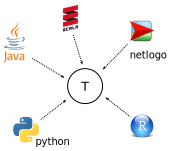
\includegraphics[width=0.4\linewidth]{task_diversity.pdf}{
		}
  \end{sidecaption}
\end{figure}


\foreignblockquote{english}[{\cite[7]{Reuillon2013}}]{In workflows, a task is an atomic execution component. Several tasks are linked with each-others by transitions to design the topology. More specifically, in OpenMOLE tasks are all portable, reentrant, immutable software components which can be run concurrently. This means that tasks have been designed so they have no interfering side effects. Therefore they can be safely dispatched on several threads, processes or computers. As far as we know, this conception of portable tasks is also a unique feature of OpenMOLE among all the workflow platforms. For us, this feature is crucial, as it makes it possible to delegate the workload entirely transparently from a user perspective, enabling the cloud aspect of OpenMOLE.}

La plus grande différence avec une chaîne de traitement classique, c'est que n'importe laquelle de ces tâches peut voir son \textbf{exécution déléguée} sur des \textbf{environnements de calcul haute performance (HPC)} de façon automatique et transparente avec (ou sans) la déclaration d'\textbf{un plan d'expérience}.

Chaque tâche comporte des \textbf{entrées} et des \textbf{sorties} en fonction du traitement. Les \textit{workflows} s'executent un peu comme un fluide que l'on aurait relâché dans un environnement contraint, en s'écoulant d'un point de départ fixé par l'utilisateur, celui-ci suivant les transitions de tâche en tâche chargées (ou charriant si l'on poursuit la métaphore) des informations qu'on lui a transmises à la fin de chaque traitement, jusqu'à parvenir à un point d'arrivée. Les valeurs des entrées sont connues au moment où la tâche est exécutée, à partir des résultats qui ont été produits et transmis au flux d'exécution par l'exécution des tâches précédentes. Car après chaque traitement, les tâches peuvent transmettre à ce flux des sorties qui seront transmises jusqu'à la tâche suivante.

Enfin, les \textit{workflows} peuvent être construits en utilisant un langage informatique dédié\Anote{dsl} (\textit{Domain Specific Language} DSL) ou composé de façon interactive et graphique en utilisant une interface utilisateur. On trouvera beaucoup plus de détails sur l'ensemble de ces concepts dans les publications associées au logiciel \autocites{Reuillon2008a, Reuillon2013}, mais également sur le \href{http://www.openmole.org}{@site} internet de celui-ci. Le mieux est encore de donner un exemple très simple et visuel de \textit{workflow} permettant d'exécuter quelques réplications d'un modèle de simulation Netlogo, comme le présente la figure \ref{fig:openmole_wfire}.

\begin{figure}[!htbp]
	\begin{sidecaption}[Exemple de plan d'expérience pour la réplication de modèle avec Netlogo]{Exemple de plan d'expérience faisant seulement varier la graine aléatoire du modèle Netlogo \foreignquote{english}{Fire}. Ce modèle de simulation très simple permet de simuler le déplacement d'un feu dans une surface boisée dont on peut faire varier la densité. C'est un exemple que l'on trouve également dans le papier \textcite{Reuillon2013}.}[fig:openmole_wfire]
	 \centering
	 \subbottom[Cette première phase de création du \textit{workflow} nécessite de paramétrer les deux premières tâches \textbf{Et (Exploration task)} et \textbf{Nt (Netlogo task)}. La tâche d'exploration \textbf{Et} nécessite le choix d'un \textit{sampling} pour ensuite être capable de générer le plan d'expérience. Le modèle Netlogo doit définir ses entrées et ses sorties : le paramètre de $density$ du modèle est fixé à une valeur de $60$, mais la \textbf{{\$seed}} doit être passée en entrée de la tâche au moment de son exécution pour que le modèle fonctionne. La sortie attendue du modèle correspond au pas de temps $t$ marquant l'extinction définitive du feu et l'arrêt du modèle : $t_{end-of-fire}$ \label{left_netlogo} ]{
	 	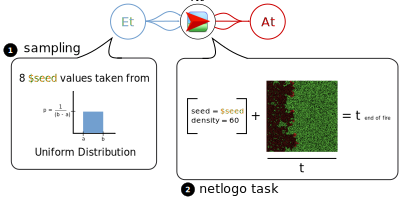
\includegraphics[width=.8\linewidth]{leftdoenetlogo.pdf}
	 	}\qquad
	 \subbottom[Le \textit{workflow} est exécuté. La première étape est de générer le plan d'expérience, c'est à ce moment là que les \textbf{{\$seed}} sont générées puis appariées avec les futures exécutions du modèle (8 seed pour 8 réplications du modèle). OpenMOLE gère toute la partie distribution des calculs, et les modèles instanciés avec les bons paramètres sont donc exécutés dans différents endroits de la planète. Une fois l'exécution des tâches achevée, les $8$ valeurs de $t_{end-of-fire}$ sont récupérées et agrégées dans un tableau par la tâche \textbf{At (Aggregation task)} \label{right_netlogo}]{
		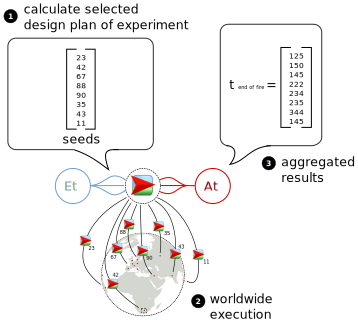
\includegraphics[width=.8\linewidth]{rightdoenetlogo.pdf}
		}
	\end{sidecaption}
\end{figure}

\paragraph {Des arguments clefs pour une première adoption du logiciel}

\begin{enumerate}[label=(\alph*),labelindent=\parindent,leftmargin=*]
\item Le moteur de \textit{workflow} permet de décrire des expérimentations avec et autour des modèles de simulation avec une grande flexibilité et une grande panoplie de \textit{task} à disposition,
\item Il est possible de créer des plan d'expériences de façon très simple, et de nouveaux algorithmes d'analyses de sensibilités sont en cours d'ajout à ce moment là du développement du logiciel.
\item Il existe déjà un plugin Netlogo permettant d'intégrer les modèles à des \textit{workflows}.
\item L'exécution de traitements naturellement parallèles (modèles de simulation ou autres) sur environnement de calcul distribué est prise en charge par le logiciel. Une capacité qui suppose pour sa mise en oeuvre des compétences techniques très particulières, que nous n'aurions jamais pu acquérir ou intégrer seul dans un logiciel, même avec l'aide du très bon manuel d'\textcite{Openshaw2000}.
\item Accès potentiel à des méthodes et des outils d'autre disciplines, OpenMOLE mutualisant les développements déjà réalisés pour l'expérimentation d'autres systèmes complexes : biologie, chimie, agroalimentaire, etc.
\item La très grande possibilité d'extension de la plateforme, appuyé par OSGI elle garantit l'indépendance de fonctionnement des composants ajoutés à la plateforme
\item La possibilité de bénéficier d'une expertise sur le calcul intensif et les outils associés
\item Le logiciel cumule déjà plusieurs années de développements, les concepts semblent robustes et déjà éprouvés dans des applications concrètes \autocite{Mesmoudi2010}.
\end{enumerate}

Le logiciel est encore dans un stade expérimental lorsque nous commencons à nous emparer des concepts pour produire nos premiers \textit{workflows}.L'interface graphique étant encore incomplète, c'est principalement par l'usage de scripts OpenMOLE que seront faites la plupart de ces expérimentations. De très nombreux aller-retour vont être nécessaires avec l'équipe des deux ingénieurs pour arriver à construire les tous premiers \textit{workflows} utilisant Netlogo, car cette tâche spécifique doit encore être confrontée à quelques cas d'utilisation imprévus (notamment sur la conversion de types entre l'API Java de Netlogo et OpenMOLE en Scala) pour que son utilisation soit vraiment exemptes de bugs.

%SimpopLocal_h3_grille.nlogo qui tourne sur la grille en juin 2010, seule la seed est amené à varier pour le moment.

Dès juin 2010 et grâce à l'obtention d'un certificat autorisant l'accès à la VO des systèmes complexes, de tous premiers \textit{workflows} mettent en oeuvre le modèle SimpopLocal dans des premiers plans d'expériences très simples, mais s'exécutant officiellement sur environnement distribué. Cette première réussite marque aussi le début d'\textbf{une remise en cause du projet de plateforme} tel qu'il a été pensé à la fin de mon stage de Master 2 en 2009, voici pourquoi.

\paragraph {Une remise en cause du projet initial}

Dans un premier temps, il est seulement prévu de s'appuyer sur OpenMOLE pour construire et exécuter des plans d'expériences de nos modèles sur environnement distribué. Le schéma alors établi est le suivant \ref{figure_schema_initial}. Nous ne passerons pas trop de temps à le décrire ici car celui-ci est devenu rapidement obsolète. Le détail du projet reste disponible dans un compte rendu annuel et dans le projet de thèse initial \autocites{Rey2010, Rey2009}.

\begin{figure}[!htbp]
	\begin{sidecaption}[Ancienne ébauche de plateforme datée de 2010]{Ebauche de la plateforme telle qu'elle est réalisée et utilisée en 2010, intégrant OpenMOLE pour les aspects distribution sur grille de calcul.}[figure_schema_initial]
	 \centering
	 	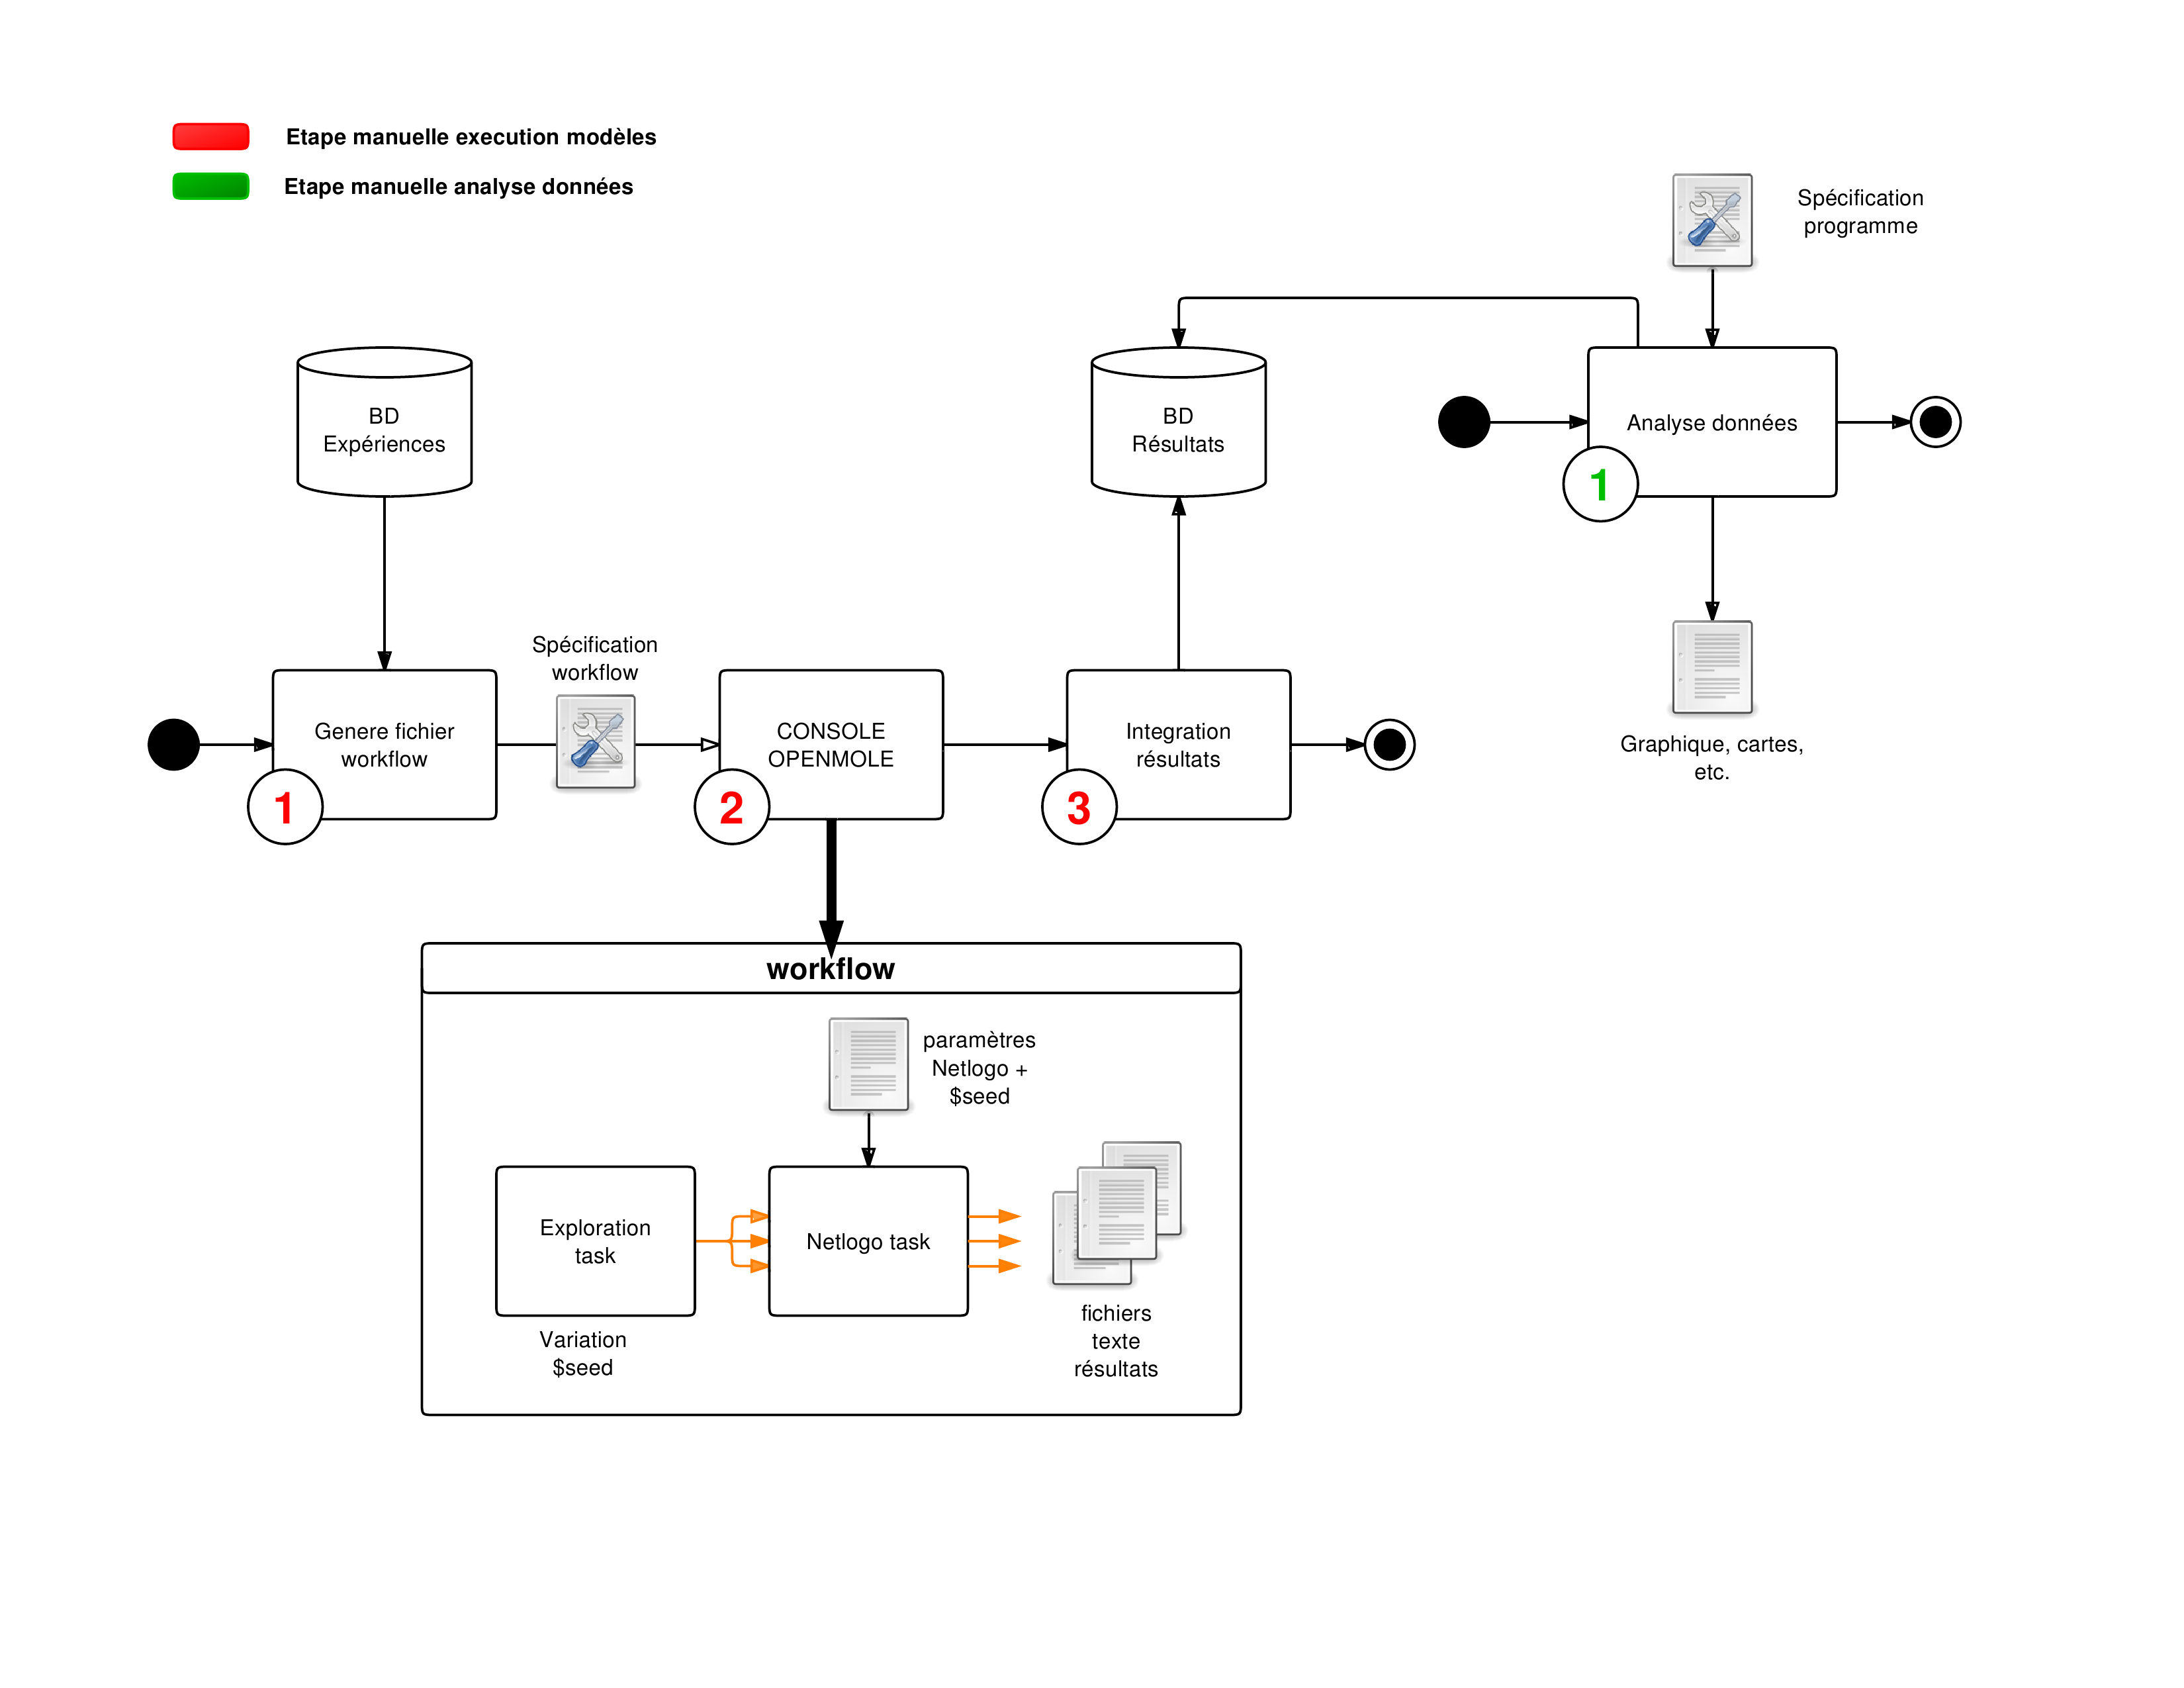
\includegraphics[width=1.0\linewidth]{oldplatform2.png}
 \end{sidecaption}
\end{figure}

Dans le projet initial, une interface logicielle doit permettre aux géographes de piloter la construction, l'exécution, et la sauvegarde des expérimentations, mais aussi la sélection et la construction de rapports automatiques à exécuter. Cela revient à construire un générateur de workflow capable d'envoyer les modèles de simulation sur grille de calcul et de stocker automatiquement les résultats dans une base de données, exploitable de différentes façons : construction de rapports automatiques, consultation des rapports sur un wiki, visualisation des données dans un SIG, etc.

Au début de l'année 2011, juste après la première campagne de calibrage du modèle SimpopLocal utilisant des algorithmes évolutionnaires (on reviendra par la suite sur cette période), il devient de plus en plus évident que non seulement l'intégration ou l'utilisation d'OpenMOLE de façon externe dans une plateforme n'est pas possible, mais qu'en plus cette solution n'est pas viable, pour plusieurs raisons :

\begin{enumerate}[label=(\alph*),labelindent=\parindent,leftmargin=*]
\item OpenMOLE est encore en plein développement, il ne sera pas stable avant plusieurs mois, notamment le DSL permettant d'écrire les \textit{workflows}.
\item Deux ingénieurs à plein temps travaillent sur le logiciel, dont le code source change tous les jours, il devient très vite difficile de suivre toutes les activités en parallèle (SimpopLocal, réalisation des workflow, réalisation des scripts pour traiter les résultats, etc.).
\item Une grande partie des outils déjà développés de mon côté sont en Python : génération de \textit{workflows} automatique, intégration des données dans une base de données, requetage de la base de données postgis, construction des rapports graphiques automatique en utilisant R et Python, etc.. La plateforme OpenMOLE est en Java/Scala, ce qui limite le dialogue entre les deux outils.
\item L'interface graphique pour la construction de \textit{workflows} contient un générateur de plans d'expériences complet et interactif. Celui-ci est - au même titre que le reste de l'interface graphique - développé par Mathieu Leclaire à plein temps, donc pourquoi redévelopper un outil similaire de mon côté ?
\end{enumerate}

Une autre évidence remet très rapidement en cause notre démarche de construction de modèle. Les premières expériences pour l'exploration du modèle SimpopLocal produisent un volume de données déjà très important, ne serait-ce qu'à cause de la stochasticité, qui nécessite de nombreuses réplications du modèle. En soit ce n'est pas vraiment un problème technique car les bases de données mises en place à cette occasion peuvent largement supporter un tel poids (quelques Gigas de données). Le problème est plutôt d'ordre méthodologique car à quoi cela sert-il de stocker un tel volume de données sur des simulations qui pour le moment ne sont pas calibrées, et sont donc destinées à être très rapidement supprimées des bases de données ? La fouille de données \textit{a posteriori} est-elle une si bonne idée dans ce cas précis ?

Prenons un exemple plus concret. Dans le cadre de SimpopLocal \autocites{Schmitt2015,Schmitt2014} un des fait stylisés recherchés par les géographes correspond à une description de la hiérarchisation du système de peuplement à un temps $t_{final}$ égal à $4000$ pas de temps (1 pas de temps = 1 année), une durée historique retenue par les experts (voir figure \ref{fig:rtstylisee}).

\begin{figure}[h]
	\begin{sidecaption}[Emergence d'une loi rang-taille dans un système de peuplements stylisé]{Emergence d'une loi rang-taille dans un système de peuplements stylisé}[fig:rtstylisee]
		\centering
		
\includegraphics[width=0.7\linewidth]{rangtaille_generique.pdf}{
		}
  \end{sidecaption}
\end{figure}

Dans une exploration \textit{a posteriori} (fouille de données), la seule façon de qualifier si la reproduction de ce fait stylisé est correcte ou pas est de soumettre aux experts les graphiques rang-taille générés. Si l'on réalise un plan complet sur les $5$ paramètres retenus pour varier dans le modèle, avec une discrétisation en $10$ valeurs sur chacun d'entre eux, et $30$ réplications, cela représente vite quelques centaines de milliers d'exécutions du modèle pour cette seule expérimentation : $10^{5} * 30 = \num{3000000}$.

Admettons que l'on puisse résumer chaque groupe de $30$ réplications dans un seul graphique comportant la moyenne, la médiane, l'écart-type, etc. cela nous laisse quand même $\num{100000}$ évaluations visuelles à expertiser. Tout cela en n'ayant aucune certitude sur la capacité de cette maille ($10$ valeurs pour chacun des paramètres, c'est très peu pour couvrir un tel espace, on en reparlera dans la section \ref{sssec:Optimisation}) à détecter la ou les zones de valeurs de paramètres qui génère correctement ce fait stylisé.

Si chaque fichier de données récupéré fait $1$ Mo, une fois multiplié par $\num{100000}$ chaque expérimentation génère environ $100$ Go de données qu'il faut récupérer, stocker, puis interroger avec les outils adéquats. Sans aucune garantie de résultat. En prenant moins de points de mesures pendant la simulation on peut revenir à des chiffres plus raisonnables, mais il faut quand même prendre en compte l'importance de cet argument.

On s'apercoit très vite que ce schéma d'expérimentation n'est pas le plus adéquat pour calibrer un modèle, même d'apparence assez simple, comme SimpopLocal. C'est un problème que nous avions déjà envisagé de façon théorique avec Thomas Louail, en reconnaissant la nécessité d'avoir des outils à notre disposition pour calibrer de façon plus automatique les modèles. Seulement en 2009, nous n'avions aucun outil fonctionnel à disposition, le stage de trois mois de A. Monzi pour développer une interface aux Algorithmes Evolutionnaires de B.Calvez n'ayant malheureusement pas abouti sur un prototype utilisable \autocite[140-141]{Louail2010}

Il se trouve que l'équipe d'ingénieurs responsable d'OpenMOLE a déjà utilisé des Algorithmes Evolutionnaires sur grille de calcul pour une problématique en agroalimentaire \autocite{Mesmoudi2010}. Or les Algorithmes Evolutionnaires sont - comme on en parlera plus en détail dans la section \ref{sec:MGO} - une des familles de techniques métaheuristiques les plus efficaces pour encadrer des problèmes d'optimisation multi-critères. Le calibrage se définit assez naturellement comme un problème d'optimisation dont l'objectif est la découverte du meilleur ajustement possible entre un jeu d'hypothèses et un jeu de critères fournis par le modélisateur. Ce type d'optimisation étant très consommateur de puissance de calcul, le couplage déjà réussi entre MGO et OpenMOLE présage d'une infrastructure technique adéquate pour la mise en oeuvre d'un projet d'évaluation systématique resté jusqu'alors très théorique (voir section \ref{ssec:evaluation_construction}).

Comme l'avaient indiqué en leur temps Diplock et Openshaw \autocite{Diplock1996}, cette possibilité de calibrer - et plus généralement d'explorer avec toutes les nouvelles méthodes HPC à notre disposition - de façon systématique et avec très peu d'efforts les modèles de simulation permet de mieux se concentrer sur la construction des modèles et des critères. Après la réalisation du premier prototype utilisant OpenMOLE, SimpopLocal et MGO, nous évoquerons comment cette approche d'évaluation systématique a continué d'inspirer des changements dans notre façon de concevoir les modèles et la modélisation. % dans le courant de l'année 2013, avec le démarrage d'une nouvelle dynamique et d'un nouveau projet de modèle de simulation.

Poursuivre le développement de cette librairie logicielle, encore instable, est très vite reconnu par les deux équipes comme un objectif d'intérêt commun. Car d'un côté il y a cette possibilité de développer un prototype de méthodologie permettant de construire et d'explorer (calibrer dans un premier temps) SimpopLocal avec des outils adaptés, réactifs, et jamais utilisés jusque là au laboratoire Géographie-cités. Et d'un autre côté, il y a la possibilité quasi-simultanée de mutualiser et donc de généraliser ces outils et cette méthodologie à n'importe quel autre modèle de simulation utilisant Netlogo et OpenMOLE.

%est  pour en faire un catalogue évolutif d'algorithmes évolutionnaires utilisables très facilement dans OpenMOLE. SimpopLocal sert de cas d'utilisation concret, mais l'horizon final est bien de permettre l'utilisation de ces outils pour n'importe quel autre modèle de simulation intégré dans un \textit{workflow}.

%Un des premier avantage à voir dans l'application de cette méthodologie réside dans l'incitation à formuler des critères qu'elle engendre chez les modélisateurs. Pour pouvoir apprendre de la dynamique des modèles mis en oeuvre, il n'y a pas d'autre choix que de formaliser les questions, les critères, que l'on veut s'attend à voir ou ne pas satisfait lors du calibrage. Cette approche à été longuemment décrit dans la section \ref{ssec:evaluation_construction}, mais aucune technique n'avait alors été évoqué pour son support.

Comme on vient de le décrire, la coopération avec l'équipe d'OpenMOLE ne va aller qu'en se renforçant au cours de l'année 2010. Le maintien de deux projets indépendants alors même que ceux-ci ont en commun un grand nombre d'idées et d'objectifs n'a plus vraiment de sens. Il aura donc fallu se déposséder d'abord de l'idée de plateforme pour l'évaluation des modèles telle que nous l'avions imaginée, pour la reconstruire à nouveau au travers d'un co-développement étroit avec des ingénieurs spécialisés dans le HPC. Une ressource informatique qui reste à ce jour le seul moyen d'explorer efficacement les modèles de simulation, et cela depuis les années 1980, date où les géographes avaient déjà pressenti la nécessité d'un tel projet (\ref{p:experience_minuit}). Une ressource indispensable mais aussi inatteignable pour un développeur seul et non spécialisé dans cette discipline. En ce sens, continuer sur ce projet de façon autonome ne fait que freiner le développement d'une coopération qui pourrait s'avérer plus fructueuse encore, car basée sur l'expertise et le travail déjà réalisé par chacun. Sans compter qu'à ce moment là le développement d'OpenMOLE laisse entrevoir des possibilités qui se situent bien au delà de ce que l'on avait imaginé dans notre cahier des charges initial.

\begin{enumerate}[label=(\alph*),labelindent=\parindent,leftmargin=*]
\item Les \textit{workflows} peuvent être sauvegardés et partagés.
\item A terme, il sera possible de \enquote{versionner}\Anote{versionnerwf} des \textit{workflows}, voire des données et des résultats \textit{associés} à ces \textit{workflows}.
\item Il existe la possibilité de proposer des \textit{workflows} de type \textit{PuzzleWorkflow}, prêt à être utilisés ceux-ci doivent d'abord être complétés ou paramétrés par l'utilisateur, comme un \textit{puzzle} dont il manquerait seulement quelques pièces pour être terminé.
\item Les concepteurs envisagent de proposer une collection de \textit{workflows} déjà prêts à l'emploi, où l'utilisateur n'aurait plus qu'à ajouter son modèle.
\item Il est possible d'utiliser et d'ajouter des tâches pour le langage R dans les \textit{workflows}, ce qui comble une partie des besoins des géographes sur le plan de l'analyse statistique.
\end{enumerate}

Tout comme son potentiel avait déjà dû apparaitre aux yeux d'Arnaud \textcite[19-26]{Banos2013} (\enquote{et si le vrai luxe c'était le calcul ?} ), il nous est  aussi paru évident qu'un tel logiciel pouvait transformer les usages d'une communauté de modélisateurs dont on a vu qu'elle était en attente de ce type d'outils depuis plus d'une decennie. Sachant que la plupart des modélisateurs actuels en sciences humaines et sociales se situent plutôt dans un entre-deux sur le plan technique (ni experts informaticiens, ni débutants), la proposition faite par les ingénieurs de l'ISC-PIF pourrait bien s'avérer être ce \enquote{chaînon manquant} qui permettrait d'enclencher une véritable démocratisation des usages du HPC pour la modélisation en géographie, et plus généralement pour la modélisation en SHS.

A partir de là, les aspects plus géomatiques prévus dans la plateforme initiale vont être mis entre parenthèses pour se concentrer principalement sur la construction d'un prototype de méthodologie d'exploration pour SimpopLocal appuyé par MGO et OpenMOLE. %De part la nature de la plateforme, dédié avant tout à la l'exploration des modèles de simulation, l'essentiel des activités de développements par se focaliser sur l'amélioration de ce processus, et va déboucher sur plusieurs innovations au croisement des différents domaines.

\paragraph {Vers la construction d'une plateforme intégrée}

Plutôt que de réinventer une nouvelle fois la roue, pourquoi alors ne pas \textbf{intégrer} les outils qui manquent aux géographes et aux modélisateurs en sciences humaines et sociales directement dans OpenMOLE, participant ainsi d'une démarche cumulative bénéfique à tous.

Si la suite de cette thèse se focalise pleinement sur la mise en oeuvre des outils et des méthodes susceptibles de fournir une évaluation plus systématique des modèles de simulations dans les \textit{workflows}, ce projet d'une plateforme intégrée d'orientation plus géomatique ne reste pas lettre morte.

L'intérêt d'une plateforme comme OpenMOLE c'est qu'elle propose une structure ouverte à l'intégration :

\begin{enumerate}[label=(\alph*),labelindent=\parindent,leftmargin=*]
\item Ajouter des connecteurs en entrées / sorties vers les bases de données. dans les \textit{workflows}
\item Ajouter une possibilité de traiter et de visualiser des données géographiques dans la plateforme (avec GeoTools, ou JTS par exemple).
\item Ajouter des tâches pour le traitement de données massives.
\item etc.
\end{enumerate}

Un autre projet d'intégration a été mené durant l'année 2013, et celui-ci a mobilisé deux stagiaires que j'ai encadrés sur 2 et 6 mois (Benjamin Bernard et Cyril Jayet). L'objectif était d'intégrer dans OpenMOLE un outil de \enquote{visualisation scientifique} pouvant être couplé de façon flexible avec les données circulant en sorties des tâches de \textit{workflows}, comme le propose la figure \ref{fig:visu_projet}. Devant les possibilités offertes par les librairies de visualisation javascript, le choix du support pour construire les visualisations (un simple graphique XY dans un premier temps) s'est porté sur un navigateur Internet. Ce projet était relativement complexe sur plusieurs aspects. Il fallait gérer l'intégration d'un navigateur Internet dans OpenMOLE, coupler un tracé des visualisations en Javascript dans un navigateur avec un flux de données en Scala, et enfin gérer l'affichage de données de façon synchrone ou asynchrone. En effet, les modèles de simulations s'exécutant sur un environnement distribué, les données sont effectivement récupérées de façon asynchrone par OpenMOLE.

\begin{figure}[htbp]
	\begin{sidecaption}[Plan d'expérience sur le modèle Netlogo Fire]{Le plan d'expérience propose de faire varier la densité du modèle de $0$ à $100$ par pas de $10$, avec $5$ réplications pour chacune de ces variations de densité. Le résultat est directement visible pendant l'exécution des simulations sur grille de calcul grâce au plugin implémenté dans OpenMOLE. Le bouton \foreignquote{english}{refresh} permet d'afficher les dernières données récupérées par OpenMOLE. Le \textit{mapping} permet de changer les variables en $x$ et $y$ en fonction des entrées et des sorties de tâches disponibles dans le \textit{workflow} : $seed$, $density$, $t_{end-of-fire}$ }[fig:visu_projet]
		\centering
		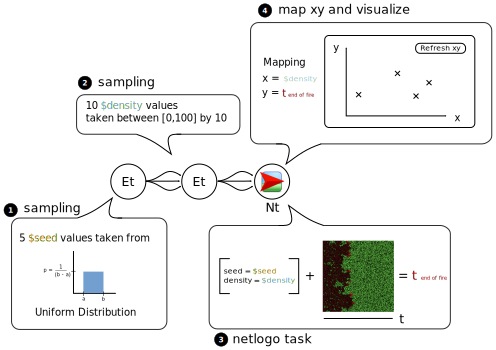
\includegraphics[width=0.9\linewidth]{leftdoenetlogo_visu.pdf}
  \end{sidecaption}
\end{figure}

Le prototype a bien été implémenté et testé avec l'aide de Robin Cura, l'auteur, et les deux stagiaires. Toutefois ce développement n'a pas pu être maintenu dans le temps. OpenMOLE disposant de sa propre autonomie et de sa propre feuille de route, les objectifs définis initialement peuvent changer très rapidement. L'interface graphique sur lequel notre prototype s'appuyait en 2013 a été abandonnée pendant plus d'un an et demi le temps de son redéveloppement et de son transfert dans un navigateur Internet. OpenMOLE devenant client/serveur, ce qui implique des changements importants d'architecture. De ce fait, les développements réalisés sur le prototype de visualisateur réalisé en 2013 doivent être revus intégralement au regard de ces changements. Ce point illustre aussi la difficulté du travail interdisciplinaire lorsque il y a un différentiel entre les équipes en termes de force de développement. Le logiciel OpenMOLE est en effet amendé tous les jours, voire plusieurs fois par jour, par deux développeurs qui opèrent sa construction à plein temps. Construire un plugin qui s'appuie sur les concepts de fond du logiciel comme on a tenté de le faire (interface graphique, implémentation interne des workflow, communication entre le coeur métier du logiciel et l'interface graphique, etc.) alors même que ceux-ci continuent d'évoluer est un travail qui peut se faire uniquement en se calant sur le rythme de développement des autres développeurs. La nouvelle interface est encore en cours de développement par Mathieu Leclaire, il faudra donc encore attendre l'officialisation et la stabilisation de celle-ci pour envisager plus sereinement la reconstruction de ce plugin de visualisation, dont l'intérêt reste entier. Plus de détails, en particulier techniques, peuvent être trouvés dans les rapports de stage de \textcite{Bernard2013} et \textcite{Jayet2013}.

\paragraph {Retour sur les étapes importantes d'une démarche prototype}

% Référence à Amblard Amblard2010 et Amblard2003 sur l'expérimentation au coeur du processus de modélisation.

Cette liste se présente comme un résumé des développements intégrant trois objets de recherche, le modèle SimpopLocal, la librairie d'algorithmes évolutionnaires MGO, et OpenMOLE.

De façon générale, les objectifs et les enjeux thématiques justifiant la création du modèle SimpopLocal sont décrits très en détail dans la thèse de Clara Schmitt \autocite{Schmitt2014} et dans un article écrit avec Romain Reuillon, Denise Pumain et Clara Schmitt \autocite{Schmitt2015}. Cette dernière publication est reproduite et complétée par quelques visuels en annexe \ref{sec:simpoplocal}.

\begin{itemize}[label=\textbullet]
%\item \textbf{1981 (CC P1)}

\item {\textbf{Janvier 2010}} Le projet de modéle multi-agents SimpopLocal commence, des réunions ont lieu tous les 15 jours environ. L'implémentation en Netlogo se fait de façon presque immédiate après quelques premières réunions.

\item {\textbf{Janvier 2010}} Rencontre avec Romain Reuillon, Mathieu Leclaire et Jérémy Fiegel à l'ISC-PIF.

\item {\textbf{Mars 2010}} Signature d'une convention devant l'intérêt commun des deux parties.

\item {\textbf{Mars 2010}} Suite aux expériences déjà réalisées de son côté avec les algorithmes génétiques, Romain Reuillon nous demande de réflechir à la formalisation des sorties de notre modèle. Autrement dit, la question \enquote{Qu'est-ce que vous voulez démontrer avec votre modèle ? } s'impose comme une question préalable à la compréhension entre les deux équipes.

\item {\textbf{Mars 2010}} Arnaud Banos demande l'inscription de Géographie-cités auprès de l'organisme de certification.

\item {\textbf{Juin 2010}} De premiers \textit{workflows} utilisant SimpopLocal sont exécutés sur la VO des systèmes complexes. Les recherches pour essayer de caractériser de façon plus automatique les sorties du modèle démarrent ce même mois.

\item {\textbf{Octobre 2010}} Première présentation du projet d'utilisation d'une grille de calcul pour le calibrage du modèle lors des journées Grid Day.

\item {\textbf{Novembre 2010}} Les premiers plans d'expériences pour explorer le modèle génèrent un grand volume de données. Même aidé par des résumés visuels, il est très difficile de faire un tri manuel à la recherche des solutions intéressantes. Il est proposé de basculer sur une évaluation des modèles de simulations a priori, en utilisant des critères quantitatifs (durée des simulations, seuil de population à atteindre) et qualitatifs (recherche d'une lognormalité dans la hiérarchisation des peuplements).

\item {\textbf{Novembre 2010} - \textbf{Janvier 2011} } Les différents objectifs pour évaluer SimpopLocal sont implémentés par Sébastien Rey dans une tâche indépendante qui peut être exécutée après la série de réplications.

\item {\textbf{Janvier 2011}} Le projet intègre l'ERC GeoDivercity obtenue par Denise Pumain. OpenMOLE devient la plateforme référente, et l'ancien projet est mis en suspens pour se concentrer uniquement sur la réalisation d'un prototype de démarche visant l'automatisation du calibrage sur le modèle SimpopLocal.

\item {\textbf{Avril 2011}} Un \textit{workflow} assez complexe (voir section \ref{p:prototype_fonctionel}) s'appuie sur la librairie d'algorithmes évolutionnaires développée à l'ISC-PIF (MGO, écrit en Scala) pour exécuter de premiers essais du calibrage du modèle SimpopLocal. A partir de cette date, l'exploration du modèle va être le moteur d'un cercle d'amélioration vertueux touchant à la fois OpenMole, MGO, et évidemment SimpopLocal dont le calibrage reste le premier objectif.

\item {\textbf{Avril 2011}} En stressant les différentes zones de valeurs de paramètres du modèle SimpopLocal, nous nous apercevons que des mécanismes de contrôle doivent être ajoutés pour limiter la saturation mémoire et processeur liée à certaines combinaisons de valeurs de paramètres. Le modèle expose une palette très variable de durée d'exécution en fonction des valeurs de paramètres, la réalisation des objectifs pouvant aller de quelques minutes à plusieurs dizaines de minutes. Le nombre d'\enquote{objet innovation} dans le modèle doit être limité par un nouveau paramètre.

\item{\textbf{Mai 2011}} Les critères retenus pour évaluer les simulations sont discutés en comité de thèse. Pour gérer l'agrégation des valeurs résultats sur les objectifs, il est choisi de privilégier l'écart absolu à la médiane (la \textit{Median Absolute Deviation} ou MAD).

\item {\textbf{Mai 2011}} La librairie pour les algorithmes évolutionnaires multi-objectifs MGO va être complètement redéveloppée en faveur d'une approche orientée composant, et de nouveaux algorithmes vont être ajoutés progressivement avec l'avancement de notre problématique d'exploration sur SimpopLocal. Ce travail est décrit dans la section \ref{sec:MGO}, il est motivé par Sébastien Rey, Romain Reuillon et Gabriel Cardoso.

\item {\textbf{Septembre 2011}} Robin Cura ajoute et expérimente un mécanisme pour déclencher des catastrophes dans SimpopLocal.

\item {\textbf{Février 2012}} Première campagne d'exploration plus conséquente du modèle, plus de $\num{50000}$ simulations sont exécutées, et les calculs durent plusieurs jours (6-7) consécutifs.

\item {\textbf{Mars 2012}} Pour essayer d'accélérer les exécutions des modèles, un plugin Netlogo est créé par Sébastien Rey et Romain Reuillon. Celui-ci tente d'exporter dans un autre langage les opérations d'échanges d'innovations entre les peuplements, une phase de tri complexe qui correspond au goulot d'étranglement limitant les performances d'exécution du modèle. Les résultats sont peu concluants et ne montrent pas une diminution des temps d'exécution satisfaisante.

\item {\textbf{Mars 2012}} Le modèle SimpopLocal est réécrit en Scala par Sébastien Rey, avec l'aide de Romain Reuillon. L'exécution du modèle est bien plus rapide (on passe de plusieurs minutes à quelques secondes) car le modèle est optimisé pour gérer les architecture multi-coeurs (ce qui n'était pas possible avec Netlogo).

\item {\textbf{Mars 2012}} Avec l'aide d'un nouveau type de \textit{workflow} paramétrable (\textit{PuzzleWorkflow}), le \textit{workflow} prototype utilisé pour calibrer SimpopLocal peut être intégré comme un \textit{workflow} générique paramétrable et donc réutilisable par tout le monde dans OpenMOLE. La définition de \textit{workflow} pour utiliser un modèle avec des algorithmes évolutionnaire passe de plusieurs centaines de lignes de script à seulement quelques dizaines de lignes.

\item {\textbf{Mars - Décembre 2012}} Comme le calibrage ne permet pas de connaître en détail la dynamique exprimable par chacun des paramètres, Romain Reuillon appuyé par Jean-Baptise Mouret (ISIR) propose une nouvelle méthode. En s'appuyant sur un objectif plus explicite de diversité, on pousse les algorithmes évolutionnaires à explorer de façon exhaustive le spectre de dynamique exprimable pour un paramètre sous contrainte des objectifs \autocite{Reuillon2015}. On obtient ainsi des profils de dynamique par paramètre, toujours en fonction d'objectifs à atteindre. La première implémentation est opérationelle en décembre 2012.

\item {\textbf{Juillet 2012}} Sébastien Rey ajoute une métrique de convergence basée sur une variante de calcul de l'Hypervolume dans MGO \autocite{Fonseca2006}. Cet algorithme nous renseigne sur l'état du volume occupé par les solutions évaluées en n-dimensions.

\item {\textbf{Juillet 2012}} Sébastien Rey ajoute l'algorithme SMS-EMOA dans MGO \autocite{Emmerich2005}. Cette variante de NSGA2 se base sur la métrique d'Hypervolume pour appuyer la sélection des meilleures solutions candidates (sur la base d'un calcul de contribution d'une solution candidate à l'expansion du volume occupé par les meilleures solutions).

\item {\textbf{Août 2012}} Romain Reuillon implémente des algorithmes évolutionnaires en \enquote{îlots} appuyé par MGO dans OpenMOLE \autocite{Whitley1997}. A la différence des méthodes classiques de distribution d'algorithmes évolutionnaires sur grille de calcul (\textit{Generational} et \textit{Steady State}), la répartition en îlot permet d'ajouter un niveau de parallélisme supplémentaire à l'exécution en faisant tourner sur chaque noeud de la grille de calcul, non pas une seule simulation, mais une population de simulations gérées par un Algorithme Evolutionnaire autonome. Les meilleurs candidats sont récoltés une fois la procédure d'évolution terminée sur chacun de ces noeud/iles. La durée des expérimentations diminue immédiatement.

\item {\textbf{Août - Décembre 2012}} La sensibilité d'une fonction objectif pose problème dans la construction d'un ensemble de solutions satisfaisant. L'epsilon dominance est ajouté en décembre dans MGO par Romain Reuillon (voir section \ref{sec:MGO} pour un exemple), ce qui règle le problème.

\item {\textbf{Octobre 2012 - Mars 2013}} Une nouvelle problématique se pose à l'équipe. Les résultats rapportés par les algorithmes évolutionnaires proposent des jeux de valeurs de paramètres de qualité très en dessous de ce qui est attendu d'une telle sélection. Après une campagne d'exploration (Sébastien Rey) dédiée à l'étude de la variabilité liée à l'aléa dans SimpopLocal, on s'apercoit que le nombre de réplications ($30$) est largement insuffisant pour que l'optimiseur puisse opérer une sélection fiable sur la base d'une médiane pour chaque objectif (voir section \ref{sec:MGO} pour un exemple). Certaines solutions ont pu être selectionnées par chance sur la base d'une bonne série de réplications, et comme l'optimiseur ne réévalue jamais les meilleures solutions selectionnées, ces solutions demeurent jusqu'à la fin de l'optimisation. $100$ réplications apparait comme un minimum, or ce n'est pas faisable, car cela multiplie la durée d'expérimentation par un facteur supérieur à deux. Une des solutions implémentées par Romain Reuillon en Mars 2013 est de rester à $30$ réplications, mais d'intégrer dans MGO une méthode de compensation de la stochasticité par une réévaluation aléatoire des meilleures solutions retenues par l'optimiseur \autocite{Pietro2004}.

\item {\textbf{Février 2013}} L'équipe présente les résultats obtenus sur SimpopLocal avec l'aide des deux méthodes d'explorations : calibrage par Algorithmes Evolutionnaires, et analyse de sensibilité en utilisant la méthode des profils.

\item {\textbf{Avril 2013}} Le modèle SimpopLocal est décomposé en briques réutilisables selon la même méthode qu'utilisée pour MGO et intègre ensuite la nouvelle plateforme de construction de modèle générique SimPuzzle. Celle-ci a pour vocation d'aide à la mutualisation des hypothèses implémentées pour les différents modèles, qui peuvent ensuite être réutilisées plus facilement dans de nouvelles compositions. L'idée d'un versionnement des hypothèses se concrétise un peu plus.

\item {\textbf{Juillet 2013}} Première soumission d'un article à \textit{Environment and Planning B} (EPB). Celui-ci fait le point sur le modèle et sur l'ensemble des développements mobilisés pour son exploration. Cette publication, reproduite en annexe (voir \ref{sec:simpoplocal}) et dans \textcite{Schmitt2015}, est l'aboutissement d'un tout premier prototype qui ouvre la voie à de nouveaux développements méthodologiques et techniques dans l'équipe ERC. On en parle plus ensuite.

\end{itemize}

Avec l'avancement des différents projets de l'ERC GeodiverCity, l'exploration des modèles devient le pilier central d'une réflexion commune qui semble rejaillir sur l'ensemble des développements, qu'ils soient thématiques, méthodologiques, ou techniques.

\subsubsection{Quatrième moment, au delà du prototype}
\label{sssec:quatrieme_moment}

\begin{figure}[t]
\begin{sidecaption}[Un schéma de synthèse pour les activités d'explorations des différents modèles de simulation dans l'ERC GeoDiverCity]{Ensemble des activités organisées autour de l'exploration des modèles de simulation. Les cercles de couleurs représentent des activités, et les flèches des relations entres les différentes activités.}[fig:S_explo_calendrier]
  \centering
 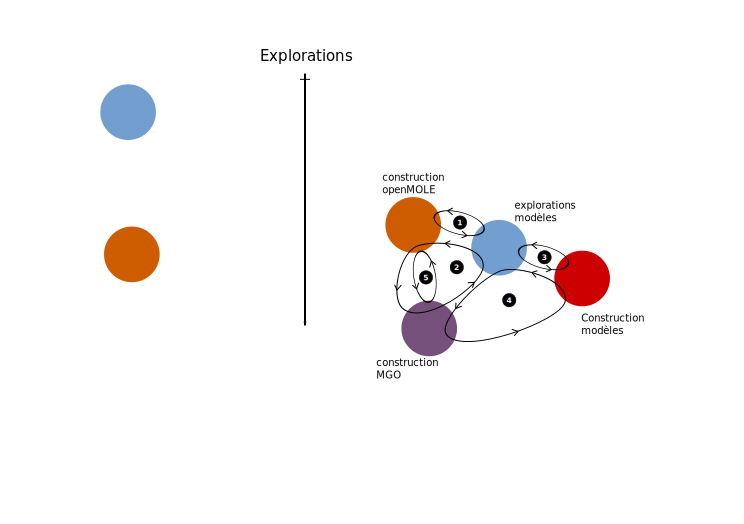
\includegraphics[width=.9\linewidth]{explorations_calendrier.pdf}
  \end{sidecaption}
\end{figure}


Le quatrième moment démarre avec la mise en route de nouveaux projets, de nouvelles dynamiques, et l'arrivée de nouvelles personnes dans l'équipe modélisation (Paul Chapron, Clémentine Cottineau, Elfie Swaerts, Guillaume Chérel). Il n'est pas possible de lister en détail l'ensemble des développements menés par cette équipe en 2014 tellement ceux-ci sont nombreux. On se contentera de nommer les projets en indiquant pour certains les avancées qu'ils représentent. Les enjeux et les challenges qui accompagnent cette interdisciplinarité vécue sont relatés plus en détail dans \textcite{Chapron2014}.

L'activité d'exploration continue d'être un catalyseur pour différents projets, c'est donc le centre de cette figure \ref{fig:S_explo_calendrier} choisie pour mettre en perspective les différentes activités passées et en cours.

\begin{myitemize2}

\item [1] \textbf{\#Exploration \#OpenMOLE} \\ Les échanges avec Romain Reuillon et Mathieu Leclaire autour de la construction de \textit{workflows} représentent plusieurs centaines d'heures de travail cumulées. Cette interaction a permis de tester, corriger, améliorer la syntaxe DSL utilisée pour décrire les \textit{workflows}, mais aussi de tester la robustesse du logiciel sur un cas d'utilisation concret, nécessitant des expérimentations de durées importantes.

\item[2] \textbf{\#OpenMOLE \#MGO \#Exploration} \\ Les différentes campagnes d'explorations menées vont avoir des retombées sur la construction de la librairie logicielle MGO, le couplage entre OpenMOLE et MGO, ce qui en retour améliore les explorations.

\begin{enumerate}
\item Intégration des algorithmes génétiques dans les \textit{workflows} OpenMOLE : \textit{EA Generational} (2011) $<$ \textit{EA Steady State} (2012) $<$  \textit{EA Island} (Août 2012) sont classés ici par degré d'utilisation du parallélisme. L'objectif est de rendre toujours plus efficientes les explorations
\item Grâce au concept de \textit{workflow puzzle}, l'écriture avec le DSL de \textit{workflows} utilisant les Algorithmes Evolutionnaires est grandement simplifiée (Mars 2012)
\end{enumerate}

\item[3] \textbf{\#Exploration \#Modeles} \\ L'exploration des résultats \textit{a posteriori} s'avère incertaine et trop coûteuse (durée d'exécution, volumes de données importants), ce qui nous renvoie à un questionnement \textit{a priori} des modèles en utilisant des méta-heuristiques.
\begin{enumerate}
	\item Réalisation du prototype de calibrage inversé utilisé sur SimpopLocal (Janvier 2010 - Juillet 2013 )
	\item Utilisation d'un nouveau type d'analyse de sensibilité avec la méthode CP-Profile (idée en Juillet 2012, réalisation Décembre 2012 , premiers résultats Février 2013 )
	\item L'exploration permet d'avoir un retour sur les hypothèses et la façon dont elles sont implémentées ( Exploration -> Modèlisation ), mais la construction modifie aussi la façon dont on va penser l'exploration : construction par incrément EBIMM \autocite{Cottineau2015}.
\end{enumerate}

\item [4] \textbf{ \#MGO \#Modeles \#Exploration} \\ Boucle liant l'activité de construction MGO, l'activité de construction du modèle, et l'activité d'exploration des modèles.

\begin{enumerate}
\item  Le développement de nouvelles méta-heuristiques pour l'exploration impacte notre connaissance des dynamiques du modèle, et donc modifie l'activité de construction des modèles.
 \begin{enumerate}
	\item Hypervolume et SMS-MOEA (Juillet 2012)
	\item CP-Profile (Décembre 2012)
	\item PSE (Janvier 2014)
	\item Epsilon Dominance (Décembre 2012)
	\item Re-Evaluation de l'archive (Mars 2013)
\end{enumerate}

\item Les modèles peuvent être amenés à être réécrits pour satisfaire des raisons de performance, ou de modularité :
\begin{enumerate}
	\item Réécriture de SimpopLocal (Mars-Avril 2012)
	\item Intégration de SimpopLocal dans SimPuzzle (Avril 2013)
	\item Réécriture de Marius pour Simpuzzle (Mai 2013)
\end{enumerate}

\item La création de SimFamilly (mai 2014) s'appuie sur MGO, OpenMOLE et SimPuzzle, et modifie profondément la façon de construire les modèles. Les modèles sont générés de façon automatique à partir des hypothèses entrées pour une famille de modèles dans SimPuzzle, l'optimiseur recherche les meilleures combinaisons d'hypothèses, et de paramètres accompagnant les hypothèses, pour ajuster les critères qu'on lui a transmis.

\item Les modèles sont également modifiés pour être utilisés par les métaheuristiques, et celle-ci mettent à l'épreuve en retour l'implémentation du modèle vis-à-vis des objectifs fixés. Ce processus intervient dans la validation interne des modèles en soulevant les erreurs, les comportements contre-intuitifs, les zones de valeurs de paramètres bloquant, ou les conditions d'arrêt trop ou pas assez strictes pour l'exploration. L'introduction d'objectifs sous forme de critères multiples pour évaluer les sorties de la simulation de façon automatique participe également de la formalisation et de la construction des connaissances, entrainant souvent pour les modélisateurs un retour sur l'empirie.
\begin{enumerate}
 \item SimpopLocal (Janvier 2010)
 \item Marius (Janvier 2013)
 \item Gugus (2014)
 \end{enumerate}
\end{enumerate}

\item[5] Boucle liant OpenMole et Mgo, le \textit{framework} est repensé pour être plus beaucoup modulaire, et donc plus facilement utilisable sous forme de tâche dans OpenMOLE (depuis Mai 2011)

\item[6] Intégration dans OpenMOLE d'un prototype d'outil permettant de construire des visualisations en temps réels sur les sorties de tâches OpenMOLE (Janvier - Septembre 2013)

\item[7]  Construction d'outils pour l'exploration des sorties de simulation des modèles réalisés
 \begin{enumerate}
 \item TrajPOP (Septembre 2011)
 \item Varius (début 2015)
 \end{enumerate}

\end{myitemize2}


% -*- root: These.tex -*-

\section{Un nouveau \textit{framework} pour systématiser l'évaluation des modèles de simulations : MGO}
\label{sec:MGO}

%%%%%%%%%%%%%%%%%%%%%%%%%%
%% NOTE CLEMENTINE
%%%%%%%%%%%%%%%%%%%%%%%%%%
% Je t'ai mis surtout des détails de forme dans le documents en pj parce que je suis incapable de juger le fond.
% Dans l'ensemble, tu avais l'air d'être inquiet de la lisibilité pour le néophyte, donc :
% - effectivement, c'est pas fastoche fastoche !
% - en fait je pense que là ou tu pourrais gagner en accessibilité (on va pas envisager le géographe des migrations en Afrique mais disons le quantitativiste moyen :), c'est sur le tout début.
% Au fur et à mesure de la lecture, on a tout les éléments on s'y retrouve et c'est intéressant et ça se lit bien.
% Par contre le début c'est chaud, et à mon avis pour deux raisons :
% - c'est la partie la plus théorique et on sent que même toi tu doutes un peu de l'intérêt de classifier les algo alors on est pas convaincu non plus et on sait pas ou ça va nous mener.
% - je pense qu'il faut que tu annonces beaucoup plus tôt, plus fort et plus souvent à quoi ça sert qu'on s'intéresse aux métaheuristiques, aux espaces de résultats et aux fronts de Pareto. Pour ne pas avoir à tout réorganiser, tu peux surement tester ce que ça donne de présenter dès le début le besoin d'algo evolutionaire en simulation géo. et comme ça on apprend plein de trucs par la suite, mais on voit ou tu nous emmènes et comment on fait notre choix parmi toutes les solutions que tu présentes...

%%et pourquoi ne pas utiliser les modèles au début pour annoncer les problèmes de modélisation et les enjeux de calibration?

%%%%%%%%%%%%%%%%%%%%%%

% Présentation de l'interet de ces techniques
% A priori déjà présenté ailleurs ?
%\subsubsection{Quelle utilité pour la construction et l'évaluation de modèle de simulation ?}

%Le chapitre 1 se terminait déjà sur la difficulté pour calibrer les modèles. Le chapitre 2 a prouvé que la construction et l'évaluation d'un modèle était deux processus indissociables,


% Fil plus chronologique, guidé par les besoins !

% - Accéder au HPC et Grid Computing
%

% - Présentation modèles exemples
% - OpenMOLE
% - MGO
%
% Plan temporaire MGO :
% - Présentation besoins / objectifs.
% - Insufisance EC existant (2.2.3.1 actuel)
% - Présentation plus large de la discipline + encadré resituant SLocal
% - Mise en oeuvre MGO
%	- Historique
%   - Principe conception innovant
% - Mise en oeuvre couplage MGO - openMOLE
% - Premier prototype, bilan autour de l'expérience SLocal

% Prise de recul sur la méthodologie, accointance et critique de la méthode POM avancé par Grimm ?

\subsection{Présentation des modèles utilisés}

Le choix est fait dans cette section de faire appel à la fois un modèle jouet (pour la compréhension générale), mais également un modèle réel (pour montrer que cela marche).

\subsubsection{Un modèle de simulation appliqué : SimpopLocal}

La présentation détaillée de ce modèle de simulation multi-agents, les problématiques qui ont motivées sa construction et son exploration, ainsi que l'analyse des résultats ont déjà fait l'objet d'une présentation détaillée à la fois dans un article EPB paru en 2015 \autocite{Schmitt2015} (joint en annexe), un article paru dans JASSS en 2015 \autocite{Reuillon2015}, mais également dans plusieurs chapitres de thèse \autocite{Schmitt2014}.

Bien que les travaux autour de ce modèle de simulation puissent apparaître comme nominatif - du fait entre autre qu'il faille bien inscrire à un moment donné ou un autre ces travaux dans une thèse - je tiens toutefois à repréciser qu'il s'agit à mon sens d'un travail partagé, ou rien n'aurait été possible sans la participation de l'un ou l'autre des collaborateurs, que cela soit dans la construction des modèles ou de certains graphiques, dans l'exploration des modèles, dans l'analyse des résultats, etc. Comme on pouvait s'y attendre compte tenu de la multiplicité de compétences nécessaires pour une telle construction, les réalisations des acteurs sont améliorés et/ou contraintes par une forme plus ou moins forte d'inter-dépendance propre à cette interdisciplinarité \autocite{Chapron2014}.

Le modèle SimpopLocal a également subi de nombreux redéveloppements, que cela soit dans sa version Netlogo (janvier 2010), Scala (avril 2012), et enfin dans son intégration dans SimPuzzle (avril 2013). En dehors des quelques évolutions de syntaxe, les \textit{workflow} utilisés pour explorer ce modèle sont quasi-similaires et cela quelque soit la version utilisée, ce qui constitue déjà en soit une preuve de robustesse de la plateforme.

Les \textit{workflows} sont disponibles sur le \href{https://github.com/ISCPIF/simpoplocal-epb}{@site} compagnon de l'article EPB, ainsi que sur le \href{https://github.com/openmole/openmole-market}{@marché} de \textit{workflows} OpenMOLE.

\subsubsection{Un modèle jouet sur les fourmis}

Le modèle de simulation \textbf{Ants} est une reproduction par \textcite{Wilensky1997} d'un modèle originellement en StarLogo en Netlogo. Celui-ci est disponible sur le \href{http://ccl.northwestern.edu/netlogo/models/Ants}{@site} de Netlogo, et par défaut dans la bibliothèque de modèle du logiciel.

\begin{figure}[H]
		\centering
	 	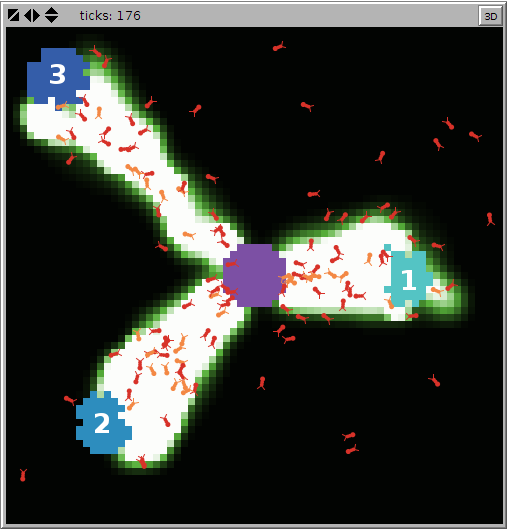
\includegraphics[width=.4\linewidth]{ants.png}
\end{figure}

Dans ce modèle Netlogo, une colonie de fourmis fourrage à la recherche de nourriture. Chaque fourmi suit un ensemble de règles simples, mais la colonie prise dans son ensemble réagit de façon complexe. Quand une fourmi trouve un morceau de nourriture, elle ramène celui-ci dans son nid, en laissant une empreinte chimique derrière elle. Lorsque les autres fourmis \enquote{reniflent} cette trace, elles suivent la piste jusqu'à la nourriture. Plus le nombre de fourmis rapportant de la nourriture vient à augmenter, plus la piste chimique est renforcée par leur passage.

Ce modèle est constitué de trois paramètres :
\begin{itemize}[label=\textbullet,noitemsep,nolistsep]
\item une $Population$ de fourmis initiale.
\item un taux $Evaporation-rate$ qui contrôle l'évaporation de la trace chimique.
\item un taux $Diffusion-rate$ qui contrôle la diffusion de la trace chimique.
\end{itemize}

\medskip

Les \textit{workflows} OpenMOLE des expérimentations présentées par la suite sont disponibles sur le site compagnon (voir notes de lecture) et sur le \href{https://github.com/openmole/openmole-market}{@marché} de \textit{workflows} OpenMOLE.

%Le \textit{\textit{framework}} MGO (Multi Goal Optimization)

\subsection{Le domaine des algorithmes métaheuristiques, une sous-discipline de l'Optimisation}

\begin{figure}[h]
\begin{sidecaption}[Vue synthétique sur les algorithmes d'optimisation]{ Vue d'ensemble des algorithmes d'optimisation repris de l'état de l'art très complet de \textcite[32]{Weise2011}}[fig:S_OverviewOptimisation]
  \centering
 
\includegraphics[width=.9\linewidth]{overview_optimisation_algorithm.png}
  \end{sidecaption}
\end{figure}

Pour mieux comprendre par la suite quelle est la spécificité des Algorithmes Evolutionnaires (\textit{Evolutionary Algorithms} ou EA), il est nécessaire de donner quelques éléments de contextes et de définitions plus généraux concernant la branche d'étude dans lesquels ceux-ci se situent. Il faut par ailleurs mettre en garde le lecteur que la plupart des définitions et des analyses présentées ici sont inspirées ou extraits d'ouvrages de synthèses à destination d'un public très large \autocites{Weise2011, Luke2013, Brownlee2012}. Par conséquent il faut garder à l'esprit que plusieurs de ces termes peuvent être discutés, enrichis, critiqués ou prendre des sens différents dans chacune des sous branches (voir figure \ref{fig:S_OverviewOptimisation}) que compte ce domaine très général qu'est l'optimisation.

\subsubsection{Q'est-ce-que l'optimisation ?}
\label{sssec:Optimisation}

Pour \textcite[22]{Weise2011}, l'optimisation \foreignquote{english}{ [...] is the process of solving an optimization problem, i. e., finding suitable solutions for it}, un problème d'optimisation nécessitant de trouver \foreignquote{english}{ [...] an input value $x^*$ for which a mathematical function $f$ takes on the smallest possible value (while usually obeying to some restrictions on the possible values of $x^*$ )}, la notation mathématique astérisque $^*$ désignant ici une valeur optimale.

Sortie de cette définition mathématique, l'optimisation peut également se définir par la mise en oeuvre d'algorithmes spécifiques. La littérature informatique met à disposition des programmeurs un ensemble d'algorithmes capables de fournir des solutions exactes dans un temps fini à un certain nombre de problèmes bien définis. C'est le cas par exemple des nombreux algorithmes de tri. Une autre classe d'algorithmes (\textit{optimization algorithms}) peut être employée lorsqu'il n'existe pas d'algorithme dédié (\textit{dedicated algorithms}), soit parce que le problème est trop spécifique, soit parce que personne n'a trouvé de solution efficace pour résoudre ce problème.

Dans ce cadre, le terme d'optimisation globale \foreignquote{english}{ [...] is optimization with the goal of finding solutions $x^*$ for a given optimization problem which have the property that no other, better solutions exist.} Le terme \enquote{global} nécessite à la différence d'une recherche qui serait \enquote{locale}, de se concentrer sur l'obtention souvent plus couteuse et plus complexe d'un optimum global, minimum ou maximum, dominant par sa qualité l'ensemble des valeurs recherchées en entrée de la fonction à optimiser.

Bien que souvent beaucoup plus lent, moins précis, et plus consommateurs de ressources que les algorithmes dédiés, ces algorithmes d'optimisation nécessitent aussi beaucoup moins d'informations pour pouvoir être exécutés : \foreignquote{english}{Most often, these algorithms only need a definition of the structure of possible solutions and a function $f$ which tells measures the quality of a candidate solution. Based on this information, they try to find solutions for which $f$ takes on the best values.} \autocite[24]{Weise2011}

Ces algorithmes s'appuient donc sur différents types de stratégies pour tirer parti du peu d'information obtenue via cette fonction $f$. De nature très diverses, on retient pour séparer une première fois ces stratégies, une typologie en deux classes.

\begin{itemize}[label=\textbullet]
\litem{\textit{Probabilistic Approaches}} Les approches stochastiques désignées dans la fig. \ref{fig:S_OverviewOptimisation} sont capables de trouver un optimum assez rapidement, mais ne peuvent pas en garantir la propriété \enquote{globale}
\litem{\textit{Deterministic Approaches}} Les approches déterministes également désignées dans la fig. \ref{fig:S_OverviewOptimisation} peuvent certes garantir au moins théoriquement l'obtention d'un optimum global, mais s'exécutent souvent au détriment d'un coût computationnel elevé.
\end{itemize}

Ces deux approches partagent également des difficultés communes, et découvrent leurs limites à des degrés divers en fonction des stratégies mises en oeuvre, dès lors que l'espace de recherche à parcourir devient trop important.

C'est le cas par exemple de l'espace de recherche de toute une sous-catégorie de problèmes \textit{NP-Complet}\Anote{np_complet_def} d'optimisation combinatoire \textit{Combinatorial Optimization Problems} (COP). Ce domaine contient par exemple les problèmes bien connus du voyageur de commerce \textit{Travelling salesman problem} (TSP), ou encore le problème du sac à dos \textit{Knapsack Problem} (KP)\Anote{note_knapsack}. Avec l'augmentation du nombre d'éléments entrant dans la définition de ces problèmes, il devient impossible de passer en revue l'ensemble des combinaisons (solutions possibles). Ce qui a pour conséquence de rendre difficile tout autant la découverte d'un optimum global, que la mesure de qualité de celui-ci, car pour établir cette dernière il nous faudrait logiquement connaitre la solution optimale, or c'est cela même que nous cherchons.

Cette première typologie recoupe une autre propriété des algorithmes. La littérature informatique qualifie ainsi d'\textit{exacts} les algorithmes dont l'exécution garantit un résultat optimum à coup sûr, d'\textit{approximate algorithms} les algorithmes capables de donner une mesure proche d'un optimum sans pouvoir en garantir la qualité, et d'\textit{approximation algorithms} les algorithmes capables de donner une mesure proche d'un optimum assortie d'une preuve de qualité. Cette dernière classe n'est pas à confondre avec une classe d'algorithmes cherchant à conserver l'optimalité en limitant par diverses stratégies le coût temporel de résolution, mais bien l'inverse, relâcher la contrainte d'optimalité, mais aussi peu que possible. Les \textit{approximations algorithms} sont une donc une sous classe d'\textit{approximate algorithms}, et constituent une branche d'étude à eux seuls, car même dans le cas de problèmes \textit{NP-Complet}, ils offrent dans des dimensions raisonnables et propres à chacun des problèmes une solution sub-optimale d'erreur mesurable et donc potentiellement améliorable, voire comparable, notamment avec les résultats donnés de façon non analytique par d'autre stratégies.
%http://en.wikipedia.org/wiki/Approximation_algorithm#cite_ref-kann92onthe_3-4

On retrouve parfois rangé \enquote{en vrac} dans la classe des \textit{approximate algorithms} la classe des heuristiques et métaheuristiques, deux termes définis plus en détail dans la section suivante.

%On nomme métaheuristique (\textit{metaheuristic}) ce type d'algorithmes s'appuyant sur des heuristiques (\textit{heuristic}).

\subsubsection{Quelle définition peut-on donner pour une heuristique (\textit{heuristic}) ? }
\label{sssec:heuristique}

Le terme heuristique \textit{heuristic} vient du Grec \textit{heuriskein} que l'on peut traduire par \foreignquote{english}{to find}, ou \foreignquote{english}{to discover}. D'usage plus large que dans la simple discipline informatique, nous retiendrons ici ce terme seulement sous son sens spécifique contextuel à l'optimisation. Rattaché à la définition d'un problème (\textit{problem dependent}), on définit une heuristique comme une mesure approximative pour définir la qualité d'une solution candidate \autocite[34]{Weise2011}.

%http://stackoverflow.com/questions/9140860/heuristic-function-for-finding-the-path-using-a-star
%http://stackoverflow.com/questions/9140860/heuristic-function-for-finding-the-path-using-a-star
%http://stackoverflow.com/questions/11779589/connection-between-a-star-search-and-integer-programming-extending-a-star
Si on se penche sur la classe d'algorithmes dédiés au problème de recherche du plus court chemin, les heuristiques sont souvent utilisées en appui des algorithmes de parcours de graphe, soit pour converger plus rapidement vers une solution optimale, soit pour justement se libérer de cette contrainte d'optimalité en visant un gain de temps au détriment de la précision. Si on prend par exemple l'algorithme de Djikstra, celui-ci n'utilise pas d'heuristique et garantit que le plus court chemin résultant sera optimal, car tous les chemins possibles entre le point de départ $A$ et le point final $B$ auront été analysés par celui-ci. Il est néanmoins connu comme étant très coûteux d'utilisation dès que le graphe dépasse un certain nombre de noeuds. L'algorithme déterministe $A^*$ s'appuie par contre sur une fonction heuristique $h(n)$ (une estimation du coût minimal reliant le noeud $n$ au noeud final) pour guider l'algorithme dans le processus incrémental de sélection d'un prochain noeud constitutif d'un chemin. En jouant sur cette heuristique, on est ainsi capable de déterminer si l'algorithme doit mettre la priorité sur la vitesse ou la précision, $h(0)$ étant équivalent ici à l'algorithme de Djikstra. Si l'heuristique est bien choisie (on dit ici que l'heuristique est admissible), alors $A^*$ garanti aussi l'optimalité du chemin trouvé, avec à la clef un coût computationnel moindre, car seule une partie des noeuds de l'ensemble du graphe auront été explorés par l'algorithme. Une autre heuristique misant plus sur la vitesse d'exécution pourra définir un chemin cette fois-ci sub-optimal avec un coût computationnel encore plus réduit. Il est à noter ici que l'utilisation d'une heuristique dans un programme n'est pas forcément motivée par la recherche d'un optimum global, mais par le gain de temps. Ainsi, un utilisateur peut très bien avoir les moyens d'obtenir un chemin optimal (Djikstra) sur une petite combinatoire de noeuds, mais peut vouloir prendre un raccourci en utilisant une méthode moins coûteuse ($A^*$). Un scénario très souvent mis en avant dans la programmation de jeux sur ordinateur, où l'on cherche régulièrement à gagner du temps, tout en se rapprochant d'un comportement faillible imitant plus un adversaire de type humain.

La forme prise par une heuristique est variable, et peut aller comme vu ci-dessus avec l'exemple $A^*$ d'une simple fonction mathématique de coût intégrée à un algorithme classique de parcours de graphes, à un algorithme beaucoup plus complexe intégrant de multiples prises de décisions pour estimer ce même coût. Dans le livre \textit{Code Complete} de \textcite[12]{McConnell2004}, celui-ci donne un exemple assez parlant pour illustrer la subtile différence qui sépare la description d'un algorithme employé au sens courant pour désigner un algorithme déterministe exact fournissant à coup sûr une solution, et la description d'un algorithme déterministe ou stochastique heuristique (ou appuyé par une heuristique) fournissant seulement un guide pour trouver, éventuellement, une solution.

\foreignblockquote{english}{Here's an algorithm for driving to someone's house: Take Highway's 167 south to Puyallup. Take the South Hill Mall exit and drive 4.5 miles up the hill. Turn right at the light by the grocery store, and then take the first left. Turn into the driveaway of the large tan house on the left, at 714 North Cedar}

\foreignblockquote{english}{Here's an heuristic for getting to someone's house: Find the last letter we mailed you. Drive to the town in the return adress. When you get to town, ask someone where our house is. Everyone knows us - someone will be glad to help you. If you can't find anyone, call us from a public phone, and we'll come get you.}

Il faut toutefois éviter de considérer les heuristiques comme appartenant à la seule classe des \textit{approximate algorithms}, car le terme ne se laisse pas facilement enfermer dans une typologie trop simple. En effet, de multiples problèmes trouvent une solution exacte jusqu'à un certain niveau de complexification, à partir duquel on fait généralement appel aux heuristiques, soit par un appel à d'autres méthodes intégrant des heuristiques, soit par une intégration d'heuristiques aux méthodes existantes. Ainsi de nombreuses classes d'heuristiques sont utilisées de façon transversale, et apparaissent donc aussi comme composantes manipulées dans la classe des \textit{approximation algorithms}. L'heuristique gloutonne \textit{greedy algorithm}\Anote{greedy_description} apparaît de façon transversale à la fois comme une solution d'approximation pour le \textit{Knapsack Problem} (KP) mais également comme moteur dans le cadre d'algorithmes déterministes exacts comme la recherche du plus court chemin de Djikstra. Un autre algorithme nommé \textit{A*} (\textit{A-Star}) qui englobe Djikstra comme cas particulier, est quant à lui capable de fournir tout à la fois une mesure exacte ou approximée en fonction de l'heuristique injectée et du niveau de complexité du problème abordé.

\subsubsection{Quelle définition peut-on donner pour une métaheuristique (\textit{metaheuristic}) ?}
\label{sssec:metaheuristique}

Le terme métaheuristique est d'origine plus moderne \autocite{Glover1986}, et a permis d'englober a posteriori des algorithmes jusque là qualifiés d'heuristiques. C'est le cas par exemple d'une bonne partie des algorithmes évolutionnaires, qui émergent principalement au cours des années 1960-1970. Cette remarque d'ordre historique est à l'origine d'une première ambiguité entre les termes à laquelle il faut encore ajouter les inquiétudes exprimées par \textcite{Luke2013}. Pour ce dernier, le terme métaheuristique est en réalité plutôt malheureux pour définir cette catégorie d'algorithmes, car contrairement à ce que laisse entendre ce terme, \textit{une heuristique pour ou à propos d'une heuristique}, ce n'est pas de cela dont il s'agit ici.

Voici comment \textcite[8]{Brownlee2012} perçoit la différence entre les deux termes : \foreignblockquote{english}[{\cite[8]{Brownlee2012}}]{Like heuristics, metaheuristics may be considered a general algorithmic \textit{framework} that can be applied to different optimization problems with relative few modifications to adapt them to a specific problem. The difference is that metaheuristics are intended to extend the capabilities of heuristics by combining one or more heuristic methods (referred to as procedures) using a higher-level strategy (hence ‘meta’). A procedure in a metaheuristic is considered black-box in that little (if any) prior knowledge is known about it by the metaheuristic, and as such it may be replaced with a different procedure. Procedures may be as simple as the manipulation of a representation, or as complex as another complete metaheuristic. Some examples of metaheuristics include iterated local search, tabu search, the genetic algorithm, ant colony optimization, and simulated annealing.}

Le terme \enquote{méta-} renvoie plus en définitive au concept générique de \enquote{stratégie de recherche} prenant la forme d'un algorithme d'optimisation capable de mélanger, manipuler des heuristiques ou d'autres métaheuristiques (cf. points \ref{enum_meta_a} et \ref{enum_meta_h})\Anote{def_meta_weise}. Contrairement aux heuristiques, les métaheuristiques se définissent plus comme un système fait de composants, dont la plasticité permet le support et l'interaction nécessaire au développement d'heuristiques plus ciblées (\textit{problem dependent})\Anote{def_meta_sorensen}. La structure offre un patron d'usage initial (\textit{pattern}) qui reste indépendant du problème abordé (\textit{problem independent}) (cf. \ref{enum_meta_g}), tout en restant évolutif, comme le montre le fort développement de cette discipline depuis les années 1980. Ce principe de flexibilité, on le retrouve par exemple dans la classe des EC, comme le mettent bien en valeur Bach, Hammel et Schwefel en 1997, dans une publication introduisant l'EC dans la série renommée des \textit{IEEE Transactions} :

\foreignblockquote{english}[\cite{Back1997a}]{We argue that the most significant advantage of using evolutionary search lies in the gain of exibility and adaptability to the task at hand, in combination with robust performance (although this depends on the problem class) and global search characteristics. In fact, evolutionary computation should be understood as a general adaptable concept for problem solving, especially well suited for solving difficult optimization problems, rather than a collection of related and ready-to-use algorithms. The majority of current implementations of evolutionary algorithms descend from three strongly related but independently developed approaches: genetic algorithms,evolutionary programming , and evolution strategies. [...] The fundamental difference in the evolutionary computation approach is to adapt the method to the problem at hand. In our opinion, evolutionary algorithms should not be considered as off-the-peg, ready-to-use algorithms but rather as a general concept which can be tailored to most of the real-world applications that often are beyond solution by means of traditional methods. Once a successful EC-\textit{framework} has been developed it can be incrementally adapted to the problem under consideration, to changes of the requirements of the project, to modifications of the model and to the change of hardware resources.}

Enfin, toujours dans une tentative de positionner ce terme dans une typologie, il faut savoir qu'une classification trop rapide de ces méthodes dans les seuls \textit{approximate algorithms} peut également être critiquée. Si les méthodes métaheuristiques sont effectivement souvent connues pour ne pas avancer de preuve, des travaux récents montrent toutefois qu'il existe de nouveaux algorithmes permettant de garantir dans certaines conditions un optimum global (CP-Algorithm de \autocite{Reuillon2015}). Tout dépend donc du degré et de la nature que l'on veut bien associer à la notion d'\textit{approximation} lorsqu'il s'agit de fournir une mesure d'éloignement de l'optimum. Les \textit{approximation algorithms} semblent toutefois plus intéressés par l'établissement d'une preuve au sens mathématique, et se concentrent avant tout sur un ensemble relativement limité de problèmes d'optimisation discret, ce qui ne semble pas être le but des métaheuristiques dans les deux cas. \autocites[1-6]{Kann1992}[13-15]{Williamson2011} %Metaheuristics: From Design to Implementation Par El-Ghazali Talbi

%You could think of a heuristic like an approximate (not approximation) solution to a problem. The difference between approximate and approximation is that the first is about getting a good guess of the solution of a problem, but that you don't really know how good it is. The second is about getting a solution for which you can prove how close it is to the optimal solution.

Enfin bien d'autres sous classifications sont possibles prenant plus ou moins en compte les spécificités propres aux différents algorithmes, comme celle opposant par exemple les stratégies utilisées en interne pour parcourir l'espace de recherche (generationel contre \textit{steady-state}, ou individuel contre populationel), la dimensionnalité possible pour la résolution des problèmes (mono-objectif contre multi-objectif), l'inspiration d'origine (naturelle biologique contre inspirations autres), etc.

Toute classification monocritère est donc rendue très difficile, une voie s'étant même ouverte pour tenter de classer ces algorithmes suivant la nature et le niveau d'opération de ces hybridations. L'origine de cette difficulté tient dans une pratique courante et assumée d'hybridation entre les différentes techniques afin de réunir le meilleur de chacune d'elles au sein de nouvelle proposition de recherche. De fait, il est important pour la suite de cerner au mieux la classe d'algorithme d'optimisation que nous allons aborder, et de définir pourquoi nous l'avons abordée. Nous nous intéresserons principalement dans la suite de cette présentation aux approches stochastiques métaheuristiques inspirées par la métaphore biologique, nommée \textit{Evolutionary Computation} (EC) ( voir figure \ref{fig:S_OverviewOptimisation}). La section \ref{ssec:EA} permettra de dégager les spécificités de cette subdivision, mais en attendant il nous faut d'abord présenter les principaux termes et concepts communs à cette classe d'algorithmes d'optimisation.

Devant la difficulté d'établissement d'une définition englobante, plusieurs auteurs semblent s'accorder pour faire du rattachement d'un algorithme à cette catégorie, une correspondance plus ou moins lâche avec un ensemble de propriétés généralement observées. En évitant une définition trop vague ou trop restrictive, on espère ainsi récupérer dans cette classe certains hybrides intéressants.

Voici un exemple de propriétés issues de \textcite{Blum2003} et traduites ci dessous :

%label=$\blacktriangleright$
\begin{enumerate}[label=(\alph*),labelindent=\parindent,leftmargin=*]
	\item Les métaheuristiques sont des stratégies qui \enquote{guident} le processus de recherche. \label{enum_meta_a}
	\item Leur objectif est d'explorer l'espace de recherche efficacement pour trouver les solutions quasi-optimales. \label{enum_meta_b}
	\item L'étendue des techniques que constitue la classe des algorithmes métaheuristiques va de la simple recherche locale à un processus d'apprentissage complexe. \label{enum_meta_c}
	\item Les algorithmes métaheuristiques sont approximatifs et la plupart du temps non déterministes. \label{enum_meta_d}
	\item Les métaheuristiques peuvent incorporer des mécanismes pour éviter d'être piégé dans une portion confinée de l'espace de recherche. \label{enum_meta_e}
	\item Les concepts de bases des métaheuristiques permettent d'adopter un certain degré d'abstraction dans la description. \label{enum_meta_f}
	\item Les métaheuristiques ne sont pas \textit{problem-specific}. \label{enum_meta_g}
	\item Les métaheuristiques peuvent faire usage d'une expertise du domaine au travers des heuristiques controlées par une stratégie de plus haut niveau. \label{enum_meta_h}
	\item La plupart des métaheuristiques actuelles font appel à une mémoire pour améliorer le processus qui guide la recherche. \label{enum_meta_i}
\end{enumerate}

Afin de mieux comprendre cette table de propriétés un peu abstraite, il est proposé de reprendre ces différents points au travers d'une lecture commentée, en commencant par une question ciblée sur la mécanique interne régissant ce type de technique.

\textit{Comment se matérialise la recherche de solutions optimisées dans une métaheuristique ?}

Si on considère les problèmes de combinatoires discrets comme \textit{TSP} ou \textit{Knapsack}, on a déjà vu que le nombre de combinaisons à évaluer lors d'une augmentation du nombre d'éléments participant à la définition du problème devient très vite problématique si on cherche à trouver une solution optimale exacte. Si on prend le cas d'un exemple plus ludique d'optimisations discrètes dans la branche des jeux (\textit{Combinatorial game theory}), le nombre de combinaisons légales possibles pour un plateau de 19 par 19 dans le jeu de GO chinois est estimé par \textcite{Tromp2007} à $2.08168199382×10^{170}$ . Même si certains auteurs comme Tromp estime qu'un tel calcul sera possible d'ici quelques mois\Anote{tromp_appel_calcul}, les problématiques posées par ce jeu mettent au défi les meilleurs programmes en intelligence artificielle \autocite{Bouzi2001}, et cela malgré des progrès spectaculaires ces dernières années, via notamment l'utilisation d'heuristique plus efficace que les approches classiques\Anote{mcts_go}.  Dans le cas d'un problème continu discrétisé, comme la recherche des meilleures valeurs de paramètres pour une simulation, la mise en oeuvre d'un plan factoriel complet (d'autres types de stratégies beaucoup plus fines existent) pose un problème double.

D'une part ce choix ne résout en rien la problématique combinatoire. Donnons un exemple plus concret, si une simulation possède $5$ paramètres, chacun de ces paramètres étant discrétisé en $10$ pas, cela nous donne déjà $10^5$ combinaisons possibles à évaluer. Si on considère que le modèle de simulation ainsi exécuté est stochastique ($10$ réplications), dans un délai relativement rapide (1 minute), la durée totale d'exécution de ce plan, pourtant relativement \enquote{grossier} d'un point de vue de la couverture de l'espace des paramètres, est environ égale à deux années de calcul... La parallélisation d'un tel calcul, c'est-à-dire son exécution sur plusieurs processeurs ou ordinateurs en parallèle, pourrait évidemment réduire ce temps de calcul à des dimensions plus raisonnables, mais c'est sans compter sur un deuxième problème, plus contraignant.

Avec le choix d'une telle maille pour la discrétisation des paramètres, c'est prendre le risque de passer à côté de solutions potentielles, une problématique contraignante d'autant plus qu'elle se complexifie avec l'augmentation du nombre de paramètres, comme le dicte le phénomène de \textit{Curse Dimensionality} établit par Richard Bellman. Ce problème est principalement d'ordre statistique, là ou $100$ points peuvent suffire dans un espace entre $(0..1)$ de dimension $1$ pour commencer à inférer ($0.01$ de distance entre chaque point), $100$ points dans un même espace $(0..1)$ de dimension $10$ ne couvrent plus qu'une toute petite partie du volume disponible. Chaque point est alors entouré d'une large portion de vide qui rend délicate toutes inférences à partir d'une si faible couverture d'un tel espace. Pour obtenir une couverture équivalente avec une distance de $0.01$ entre chaque point, il faudrait disposer de $10^{20}$ points, ce qui semble considérable \autocite{Bellman1961}. On peut voir un peu mieux sur l'illustration \ref{fig:curse} les effets d'un tel phénomène.

\begin{figure}[htbp]
	\begin{sidecaption}[Le problème de la Curse Dimensionnality]{Illustration des effets de la \textit{Curse Dimensionality} sur un plan d'expérience de 9 points entre 0 et 1 exclus. }[fig:curse]
	 \centering
	 	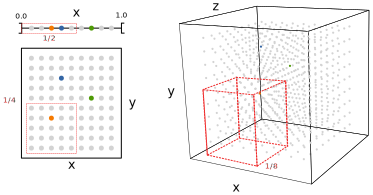
\includegraphics[width=.9\linewidth]{plot3d.pdf}
	\end{sidecaption}
\end{figure}

\begin{testiv}{Curse Dimensionality}{Exemple de Curse Dimensionality avec Simpop Local}

Le tableau ci-dessous présente le domaine de variations retenue par les experts pour les 5 paramètres du modèle agent Simpop Local, ainsi que le domaine de variation extrait de l'ensemble des meilleures valeurs de paramètres trouvées lors du calibrage \autocite{Schmitt2014, Schmitt2015}.

\begin{table}[H]
\centering
\begin{tabular}{@{}lll@{}}
\toprule
                   & Explored Domain & Solutions Domain          \\ \midrule
$P_{creation}$     & {[}0,1{]}       & ~{[} \SI{1.1e-06} ; \SI{1.3e-06} {]} \\
$P_{diffusion}$    & {[}0,1{]}       & ~{[} \SI{6.7e-07} ; \SI{6.9e-07} {]} \\
$InnovationImpact$ & {[}0,2{]}       & ~{[} \SI{7.7e-03} ; \SI{8.4e-03} {]} \\
$DistanceDecay$    & {[}0,4{]}       & ~{[} 0.66; 0.75 {]}       \\
$R_{max}$          & {[}1,40000{]}   & ~{[} 10090; 10465 {]}     \\
Volume             & 320000          & ~ \SI{4.7e-16}{}               \\ \bottomrule
\end{tabular}
%\caption{Valeur }
%\label{my-label}
\end{table}
Quelque soit finalement la résolution du plan d'expérience envisagé par l'utilisateur, celui-ci n'avait dans ce cas là que peu de chances de soulever l'existence d'une zone de solutions potentielles dans un espace de résolution aussi fin; seule l'usage d'une méta-heuristique pouvait détecter cette zone de validité du modèle, dans un volume qui représente au final $\SI{4.7e-16}{} / \num{320000} = \SI{1.5e-21}{} $ du volume total.

\end{testiv}


% Exemple pour illustrer ca au travers des problèmes SLocal qu'on a eu ?

% Jonction des trois fonctions objectifs

% Plutot une argumentation pour justifier de la nécessité d'explorer rapidement les modèles. Mais dans un deuxième temps, sur les analyses de sensibilités, car analyse de sensibilité c'est pas tip top

Contrairement à d'autres méthodes d'optimisations, les métaheuristiques font généralement appel à un processus d'échantillonnage (voir point \ref{enum_meta_b}) pour explorer de façon stochastique un espace de recherche de toute façon beaucoup trop vaste pour être parcouru de façon exhaustive. Cela permet de repousser en partie ce problème de couverture de l'espace de paramètres lié à l'augmentation de la dimensionnalité du problème, car nous verrons que les méta-heuristique opérant dans des espace de paramètres discrets mais aussi continus, sans qu'une discrétisation préalable soit nécessaire en amont.

C'est pour cela que \textcite[7]{Luke2013} nous propose de voir ce type de problème autrement, partant du postulat assez logique qu'une solution \enquote{même non optimale} est un point de départ pour l'amélioration de toute façon bien meilleure que \enquote{pas de solution du tout}.

\foreignblockquote{english}[{\cite[7]{Luke2013}}]{ Metaheuristics are applied to \enquote{I know it when I see it} problems. They're algorithms used to find answers to problems when you have very little to help you: you don't know what the optimal solution looks like, you don't know how to go about finding it in a principled way, you have very little heuristic information to go on, and brute-force search is out of the question because the space is too large. But if you're given a candidate solution to your problem, you can test it and assess how good it is. That is, you know a good one when you see it.}

Suivant ce raisonnement, la connaissance d'un problème se construit au travers d'une confrontation répétée de nos représentations, de nos interrogations avec la forme réelle et encore inconnue prise par celui-ci\Anote{paul_rationalite}. La carte de ce nouveau territoire se révélant peu à peu dans la projection sur l'espace des solutions des choix effectués lors de la sélection des nouveaux candidats à évaluer (solutions candidates).

Les métaheuristiques sont donc là pour faciliter l'exécution de cette tâche complexe et répétitive qui consisterait à améliorer notre connaissance du problème en proposant de façon pertinente de nouvelles solutions candidates à évaluer, ces dernières étant choisies si possible en fonction des résultats obtenus par les précédentes (voir point \ref{enum_meta_i}). La perspective d'une telle automatisation pose évidemment un certain nombre de questions.

Quels sont les choix mis à disposition de l'optimiseur pour améliorer la réponse attendue des solutions candidates entre chaque incrément ? \autocite[19]{Weise2011}

Une comparaison automatisée nécessite pour être mise en oeuvre de définir \begin{enumerate}[label=(\alph*)]
\item sur quelle base se fonde l'évaluation d'une solution,
\item la comparaison entre les solutions évaluées,
\item et la sélection de nouvelles solutions candidates.\end{enumerate}

Car l'optimiseur, tout comme nous, ne connaît pas directement la forme prise par l'espace des solutions, et doit bien concevoir en interne les choix permettant, par la sélection de nouvelles solutions candidates à évaluer, de progresser si possible vers une solution optimum.

De fait dans un tel scénario, et pour éviter une recherche aléatoire, l'évaluation de solution candidate renvoie à l'existence d'une expertise externe à l'optimiseur, le seul capable de formaliser ce qui différencie une bonne solution d'une mauvaise solution. On revient à parler ici d'heuristique, et de leurs diversités, car si celles-ci interviennent dans l'évaluation des solutions candidates (a), elles interviennent aussi dans les autres cas (b) et (c). Elles se présentent sous la forme de différents types de connaissances, interrogent différents espaces, et s'intègrent souvent sous la forme de composants dans la structure plastique des métaheuristiques.

L'injection de connaissances (voir point \ref{enum_meta_h} ) dans ce type d'algorithme métaheuristique est donc double, et opère à la fois de façon précise dans la formalisation d'un ou de plusieurs critères qui vont servir pour l'algorithme optimiseur à déterminer la qualité, bonne ou mauvaise, d'une solution candidate; et de l'autre elle intervient cette fois ci de façon moins contrôlable dans la façon dont l'expérimentateur va construire et paramétrer une métaheuristique pour l'adapter au mieux à son problème. La qualité interne (paramètre, structure) de la métaheuristique définit aussi en quelque sorte le processus d'exploration, ce qui explique aussi la dépendance de ce type d'algorithmes à l'environnement qu'ils doivent explorer.

\begin{figure}[!htb]
	\begin{sidecaption}[Projection de solutions candidates dans l'espace des objectifs]{Projection du vecteur de solution candidates $\{a \dotsc n\}$ dans l'espace des objectifs. Les flèches indiquent dans quel sens et sur quel plan se fait la projection des points. Les couleurs permettent de repérer quelle est la ligne de points que l'on a projetée, de la ligne 1 à 3 sur $(x,v)$ et de la ligne 1 à 4 sur $(y,v)$}[fig:spacePspaceOmultimodal]
	 \centering
	 	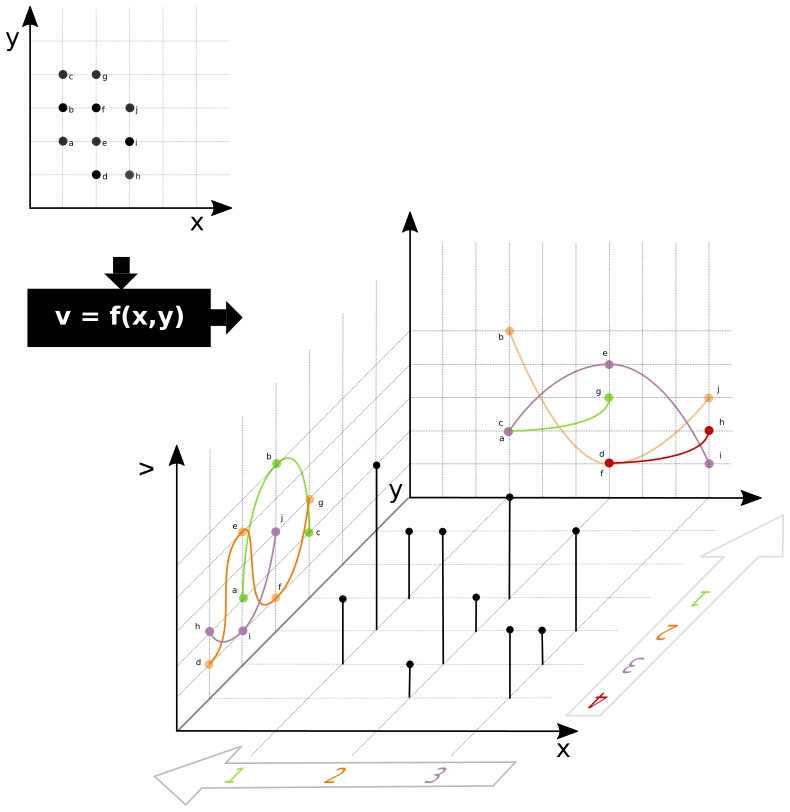
\includegraphics[width=.9\linewidth]{espaceP_espaceO_multimodal.pdf}
	\end{sidecaption}
\end{figure}

L'objectif est rendu complexe car la relation entretenue entre ces deux espaces, celui des solutions candidates disponibles, et celui des évaluations est bien souvent dissymétrique. Pour mieux comprendre cette relation, la figure \ref{fig:spacePspaceOmultimodal} illustre cette correspondance des solutions candidates $\{a \dotsc n\}$ décrites par leurs coordonnées $(x,y)$ lorsqu'elles sont projetées dans l'espace des objectifs $\mathbb{Y}$ en suivant la transformation attendue par la fonction boîte noire de dynamique non linéaire $f(x,y)$. Les valeurs $v = f(x,y)$ des différentes solutions candidates sont également projetées sur le plan 2D $(x,v)$ et $(y,v)$ pour mieux visualiser la forme prise par cette surface en 2D.

Pour visualiser la valeur $v$ prise par chacune des solutions candidates, on projette celle-ci dans l'espace $(x,y)$, ce qui nous permet de mieux constater l'éclatement des valeurs de $v$ sur la figure \ref{fig:xyspacePspaceOmultimodal}.

\begin{figure}[htbp]
	\begin{sidecaption}[Représentation des solutions candidates sur plusieurs plan vis-à-vis de la fitness]{Les couleurs indiquent la valeur $v = f(x,y)$ de chaque solution candidate $\{a \dotsc n\}$. $(v,x)$ et $(v,y)$ sont les plan extrait de la figure \ref{fig:spacePspaceOmultimodal}. On cherche ici à minimiser la valeur de $v$ :
\parbox{\marginparwidth}{
\begin{enumerate}[label={},labelindent=0pt,leftmargin=*]
        \item \sqbox{tangoBlue1} indique une fitness minimale, cf. qui maximise $v$
        \item \sqbox{tangoOrange1} indique une fitness intermédiaire et,
        \item \sqbox{tangoRed1} indique une fitness maximale, cf. qui minimise $v$
\end{enumerate}}}[fig:xyspacePspaceOmultimodal]
	 \centering
	  \subbottom[\label{subfig_xyespaceSolutionCandidate_a}]{
	 	
\includegraphics[width=0.4\linewidth]{xyespaceSolutionCandidate_a.pdf}
	 	}
	 \subbottom[\label{subfig_xyespaceSolutionCandidate_b}]{
	 	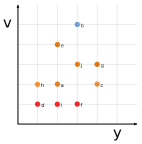
\includegraphics[width=.4\linewidth]{xyespaceSolutionCandidate_b.pdf}
	 	}
	 \subbottom[\label{subfig_xyespaceSolutionCandidate_c}]{
		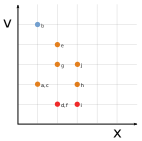
\includegraphics[width=.4\linewidth]{xyespaceSolutionCandidate_c.pdf}
		}
	\end{sidecaption}
\end{figure}


\begin{figure}[!htbp]
	\begin{sidecaption}[Déplacements simultanés dans l'espace des solutions candidates et dans l'espace des objectifs]{Représentation de deux déplacements dans l'espace des solutions candidates et son équivalent dans l'espace des objectifs
	\parbox{\marginparwidth}{
	\begin{enumerate}[label=(\alph*),labelindent=\parindent,leftmargin=*]
	        \item Partant de $b$, on se déplace d'une unité vers $c$ ou $a$, ce qui dans l'espace des objectifs équivaut également à un déplacement vers $h$; $v=2$ pour $v_h, v_a, v_c$
	        \item Partant de $b$, on se déplace toujours d'une unité vers $f$, ce qui dans l'espace des objectifs équivaut également à un déplacement vers $d$ et $i$; $v=1$ pour $v_d,v_i,v_f$
	\end{enumerate}}}[fig:xytrajectoire]
	 \centering
	  \subbottom[\label{subfig_xytrajectoire_a}]{
	 	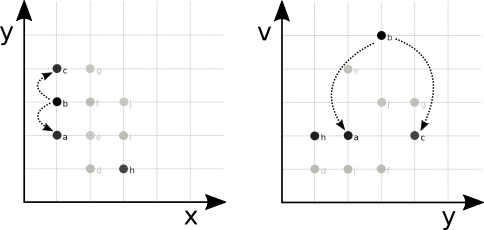
\includegraphics[width=0.8\linewidth]{xytrajectoire_a.pdf}
	 	}\qquad
	 \subbottom[\label{subfig_xytrajectoire_b}]{
	 	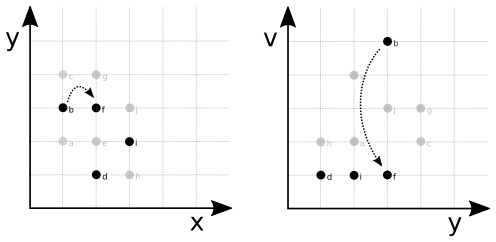
\includegraphics[width=.8\linewidth]{xytrajectoire_b.pdf}
	 	}
	\end{sidecaption}
\end{figure}

Deux solutions proches dans l'espace des solutions candidates peuvent amener à des résultats très différents, et inversement, pour deux évaluations proches peuvent correspondre des solutions candidates très éloignées, comme le détaille la figure \ref{fig:xytrajectoire}. Il s'agit d'une propriété bien connue des fonctions non linéaires, qu'elles soient décrites de façon explicite via le formalisme mathématique, ou de façon implicite dans l'expression des dynamiques complexes de modèles de simulation.

Il est clair que l'information récoltée par un tel déplacement basé sur une distance euclidienne dans le plan $(x,y)$ n'est pas pertinent dans la recherche des emplacements possibles des meilleures solutions (voir figure \ref{fig:xytrajectoire}). Il semble par exemple plus intéressant pour l'optimiseur d'accéder aux solutions par le prisme d'ensembles construits sur la base d'une valeur $v$ commune (voir figure \ref{fig:xyspacePspaceOmultimodal}). Une information qui peut être exploitée de multiples façons, toujours en permettant à l'optimiseur de déterminer un nouvel ensemble de solutions candidates à évaluer.

Si l'obtention d'une cartographie complète d'un tel espace de solutions peut être l'objectif de ce type de raisonnement, la recherche d'un optimum en est un autre. Dans un cas on aura tendance à maximiser la diversité dans le choix de solutions candidates à évaluer, afin d'essayer de couvrir au mieux le territoire à explorer. Cette idée on la retrouve dans l'établissement d'une \textit{fitness landscape}, ou dans sa version multi-objectif, d'un \textit{problem landscape} \autocite[93-94]{Weise2011}, un paysage cumulé de l'espace des objectifs indiquant toutes les valeurs prises par ceux-ci au cours de l'exploration\Anote{paysage_cumule}. Un espace mis à profit par l'optimiseur pour améliorer la proposition de solution candidate, par exemple en se basant sur la construction de cluster de valeurs intéressantes comme indiqué précédemment, ou encore en cherchant à favoriser les zones de cet espace encore peu explorées, etc. Alors que dans le cas d'une optimisation pour la calibration ou la prédiction, trouver le plus rapidement possible un minimum local ou global peut constituer un objectif suffisant.

En réalité, ces deux objectifs sont souvent liés, et c'est souvent l'expertise humaine intervenant de façon externe à l'optimiseur qui va déterminer l'importance de l'un ou de l'autre dans la stratégie à suivre. Dans le cas par exemple d'une optimisation de paramètres nécessaire à la marche efficiente d'une centrale nucléaire, la découverte d'un minimum local robuste peut s'avérer beaucoup plus intéressante qu'un minimum global instable. La topologie proche de l'espace des solutions déjà exploré peut constituer un facteur de connaissance d'intervention plus ou moins importante dans l'expertise d'une bonne ou d'une mauvaise solution.

Cette mécanique on la retrouve également à un autre niveau, dans le fonctionnement interne des métaheuristiques. En effet, celles-ci s'appuient le plus souvent sur la métaphore biologique évolutive pour mettre en tension une recherche de solutions guidée toute à la fois par l'\textit{exploration} (trouver des solutions originales), et l'\textit{exploitation} (améliorer les solutions existantes).

\begin{figure}[!htbp]
\begin{sidecaption}[Recherche d'un minimum global]{Recherche d'un minimum global.}[fig:hmap2ab]
 \centering
 \subbottom[Une fonction $f(x)$ présentant un unique minimum global.\label{subfig_hmap2ab_a}]{
 	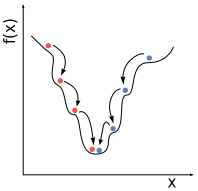
\includegraphics[width=.4\linewidth]{heightmap2a.pdf}
 	}\qquad
 \subbottom[Une fonction $f(x)$ présentant un minimum local et global.\label{subfig_hmap2ab_b}]{
	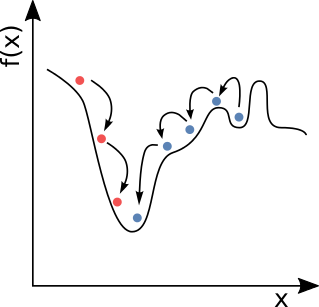
\includegraphics[width=.4\linewidth]{heightmap2b.pdf}
	}
\end{sidecaption}
\end{figure}

Les opérateurs intervenant comme stratégies dans la médiation de ces deux concepts sont conçus pour éviter à l'optimiseur un certain nombre d'écueils. Trop longue pour être abordée ici de façon exhaustive, cette liste évoquant les problèmes et solutions qui résultent du rapport entre les formes de problèmes abordés et les faiblesses génériques ou dépendantes des métaheuristiques utilisées, \textcite{Weise2011} en donne une description experte sur une centaine de pages. On peut également se référer à une autre synthèse, abordant ces problèmes avec un angle un peu plus spécifique aux algorithmes évolutionnaires, réalisée en 2001 par \textcite[316-445]{Deb2001}.

En se limitant aux pièges dépendant de la topologie de l'espace des solutions (voir point \ref{enum_meta_e}), \textcite[140]{Weise2011} a proposé un tableau synthétique dont on extrait ici quelques exemples légèrement modifiés pour éclairer notre argumentaire. Les exemples des figures \ref{fig:hmap2ab} et \ref{fig:hmap2cd} mettent en oeuvre un optimiseur générant de façon incrémentale de nouvelles solutions, chacune représentée par un point. Il faut donc lire ces exemples en tenant compte du fait qu'ils présentent une représentation cumulative des différents points parcourus dans le temps par l'optimiseur.

La figure \ref{fig:hmap2ab} démontre un fonctionnement normal de l'optimiseur, capable quelque soit son placement initial (rouge ou bleu), de trouver le minimum global d'une fonction relativement simple \ref{subfig_hmap2ab_a}. Un comportement équivalent est observable dans la figure \ref{subfig_hmap2ab_b}, le compromis \enquote{exploitation - exploration} étant suffisant pour que l'optimiseur bleu surmonte l'obstacle posé par la présence d'un minimum local dans cette fonction.

\begin{figure}[!htbp]
  \begin{sidecaption}[Des fonctions difficiles à optimiser du fait de paysages complexes]{Deux types de fonctions sont rendues difficiles à optimiser du fait d'une topologie marquée.}[fig:hmap2cd]
  \centering
  \subbottom[Une fonction $f(x)$ multimodale acceptant plusieurs minimum locaux, et un seul minimum global.\label{subfig_hmap2cd_c}]{
  	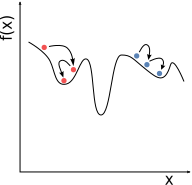
\includegraphics[width=.4\linewidth]{heightmap2e.pdf}
  	}\qquad
  \subbottom[Une fonction $f(x)$ contenant très peu d'information de gradient pour guider l'optimiseur.\label{subfig_hmap2cd_d}]{
	
\includegraphics[width=.4\linewidth]{heightmap2c.pdf}
  	}
 \end{sidecaption}
\end{figure}

A l'inverse, on perçoit bien sur ce schéma \ref{subfig_hmap2cd_c} quel effet peut avoir un déséquilibre entre les deux stratégies, une exploitation trop appuyée au détriment de l'exploration amenant souvent à une convergence\Anote{def_convergence} prématurée, c'est-à-dire à un piège dans un optimum local.

La figure \ref{subfig_hmap2cd_d} montre également que face à une topologie de fonction présentant un plateau relativement uniforme, l'optimiseur sera en peine pour trouver un minimum, même local. Un paramétrage différent de l'exploration pourra peut être résoudre ce problème, sans pour autant que l'on en soit sur.

Ce qui nous permet d'évoquer une faiblesse connue des métaheuristiques, héritée des remarques déjà faites sur les algorithmes d'optimisations stochastique\Anote{stochastic_note} dans laquelle on les place habituellement. La découverte garantie d'une solution globale optimale est en général difficile avec ce type d'algorithmes (voir point \ref{enum_meta_d})\Anote{equipe_mixite}, au moins pour deux raisons :

\begin{enumerate}
\item la variabilité qui opère lors de la sélection des solutions candidates à un instant $t$ ne permet pas de garantir qu'il n'existe pas quelque part une solution candidate sélectionée à $t+1$ dont l'évaluation révélera un meilleur optimum. La définition d'un critère d'arrêt est donc rendue délicate.
\item La variabilité dans l'établissement d'une trajectoire de recherche implique qu'un algorithme de même qualité puisse passer une première fois à côté d'un optimum, et une deuxième fois trouver celui-ci.
\end{enumerate}

\begin{figure}[!htbp]
\begin{sidecaption}[Représentation de la navigation indirecte d'une métaheuristique dans un espace de solution]{Représentation d'une navigation indirecte de l'optimiseur dans un espace de solution $z = f(x,y)$.}[fig:hmap1]
  \centering
  \subbottom[\label{subfig_hmap_a}]{
  	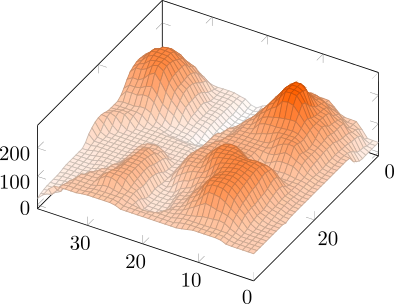
\includegraphics[width=.4\linewidth]{heightmap1a.png}
  	}\qquad
  \subbottom[\label{subfig_hmap_b}]{
	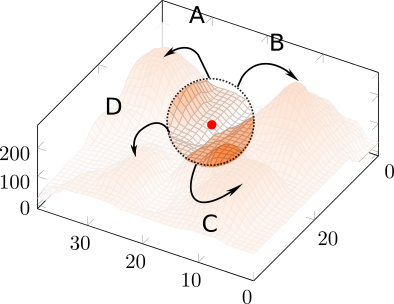
\includegraphics[width=.4\linewidth]{heightmap1b.png}
  	}
\end{sidecaption}
\end{figure}

Pour mieux comprendre les problèmes posés par des espaces de solutions multi-modaux, déjà figurés en deux dimensions dans \ref{subfig_hmap2cd_c}, on représente cette fois ci dans la figure \ref{fig:hmap1} l'optimiseur dans un espace en trois dimensions similaire à celui vu dans la figure \ref{fig:spacePspaceOmultimodal}, à la recherche d'un optimum global. La fonction ainsi représentée comporte deux entrées $(x,y)$, et une sortie $z = f(x,y)$ représentant la valeur numérique résultat de l'optimisation.

Attention à la lecture de ces schémas, il ne faut pas oublier que l'optimiseur \textbf{ne se déplace pas directement} sur le terrain visible dans la figure \ref{subfig_hmap_a}, et pour laquelle celui-ci n'a justement aucune visibilité. C'est un peu comme visualiser un labyrinthe de l'extérieur sur une feuille, puis de l'intérieur quand on s'y projette, la difficulté pour résoudre celui-ci n'est plus la même. La visibilité dont dispose l'optimiseur est celle des résultats de solutions candidates déjà évaluées (voir point \ref{enum_meta_i}). Il s'agit donc de proposer de nouvelles solutions candidates soit en les composant à partir d'une manipulation des solutions candidates déjà évaluées, soit en introduisant de toutes nouvelles solutions candidates prises de façon aléatoire. Au cours de l'itération mesurant la progression de l'algorithme, c'est bien l'évaluation de cette nouvelle population de solutions candidates qui détermine s'il y a effectivement eu un déplacement qualitatif dans l'espace des solutions evaluées. Le déplacement du point rouge dans cet espace n'est donc effectif que si on trouve à un instant $t + 1$ une solution plus intéressante qu'à l'instant $t$.

A partir des résultats de la première solution candidate évaluée figurée ici en rouge dans \ref{fig:hmap1}, les opérateurs de recherches soumis à l'aléa d'une recomposition ou d'un tirage aléatoire peuvent tout à fait proposer un candidat à $(x,y)_{t+1}$ qui débouche sur un résultat $z = f(x,y)$ plaçant l'optimiseur dans le sillon d'un gradient de pente parmi plusieurs. Ce qui mènera probablement l'optimiseur à découvrir des optimums de qualités très différentes : $A$ (local), $B$ (global), $C$ (local), $D$ (local).

Autrement dit, en plus de la stochasticité inhérente de ces algorithmes, non seulement un algorithme de type $A$ n'aura pas les mêmes résultats qu'un algorithme de type $B$, mais celui-ci sera également différent d'un algorithme $A'$ du fait d'un paramétrage différent.

Comme déjà évoqué dans les différentes définitions, on retrouve ici la qualité de flexibilité des métaheuristiques, permettant de transformer ce qui pourrait de prime abord paraître pour un défaut, en qualité. L'utilisation de celle-ci permettant d'étendre toujours un peu plus leurs champs d'utilisation, en facilitant la réponse aux questions suivantes\Anote{q_ppr} :
\begin{enumerate}
\item  \foreignquote{english}{What parameter settings do I use to get good results when applying heuristic method X to problem Y?}
\item  \foreignquote{english}{How do I adjust the parameters of heuristic X so I get better results on problem Y?}
\item \foreignquote{english}{Which is \enquote{better}, heuristic X or heuristic Y?}
\end{enumerate}

On pourrait ainsi ne retenir que cette citation de source inconnue, lorsqu'elle définit une métaheuristique comme \foreignquote{english}{ a pretty good rule for finding pretty good rules.}

Cette flexibilité vient compléter et compenser efficacement cet horizon de connaissance assez limité, nécessaire à une généricité d'emploi. Les métaheuristiques fournissent ainsi le support générique initial pour en faire un outil d'usage indépendant du problème, tout en fournissant les outils pour favoriser également leur propre modification en vue d'une amélioration de résultat pour un problème donné. Elles cumulent donc ces deux propriétés de dépendance et d'indépendance face à un problème donné.

De plus, la recherche dans cette discipline ne se contente pas d'organiser une forme de compétition qui mènerait à elle seule, par l'apprentissage répété de fonctions aussi standardisées que celles utilisées dans les figures précédentes, à une surestimation de certains algorithmes\Anote{test_fonction_surutilisation}, et se nourrit également d'une recherche plus appliquée à des problématiques réelles. Ce qui permet par effet retour, d'espérer voir appliquer à des formes de problèmes génériques, des opérateurs dédiés à l'origine à des problématiques spécifiques. La construction et l'évaluation d'heuristiques plus performantes servant indirectement une cause plus générale.

Enfin, une des propriétés qui n'a pas encore été introduite dans ce résumé est la capacité de notation et de description abstraite des métaheuristiques (voir point \ref{enum_meta_f} ). Des concepts de plus haut niveau sont introduits pour désigner l'expression et la manipulation d'heuristiques et de classes d'heuristiques dans un système composant la métaheuristique. Mais avant de pouvoir introduire ces subtilités de typologie propre à chaque classe de métaheuristique, il faut également rappeler l'existence d'une base commune de formalisation mathématique permettant la description des problèmes. Autrement dit, cela revient à introduire ou à poser sur une partie des mots déjà utilisés dans cette section, un certain nombre de notations mathématiques d'utilisation relativement standard dans cette communauté informatique utilisant les métaheuristiques.

Il nous restera également à aborder dans la section suivante, la question des \textbf{moyens} mis à disposition de l'optimiseur pour opérer la sélection de nouveaux candidats à évaluer. Jusqu'ici seule une représentation de ces solutions candidates dans l'espace des solutions candidates possibles a été abordée, ainsi que l'espace contenant les résultats des solutions candidates évaluées. Mais ces deux espaces ne constituent pas les véritables espaces sur lesquels l'optimiseur est amené à travailler, et cela bien qu'il puisse les intégrer à son expertise pour séléctionner de nouveaux candidats à l'évaluation\Anote{remarque_section_metaheuristique}.

L'introduction d'un nouvel \enquote{espace de recherche} est nécessaire, et  correspond à la somme des entrées, des paramètres, sur lequel l'optimiseur va pouvoir jouer directement, afin de modifier cette fois-ci indirectement l'expression de la solution candidate ensuite évaluée.

Autrement dit, il faut retenir qu'une solution candidate fait partie d'un espace de solutions candidates possibles, et que l'exploration de ce dernier est dépendante des bornes fixées par l'expert pour délimiter l'espace de recherche de chacun des entrants. L'objectif étant notamment de limiter le champ de recherche de l'optimiseur à des valeurs empiriquement et théoriquement possibles. Ce qui introduit aussi la possibilité d'un nouveau \textit{mapping} entre les valeurs de ces deux espaces, de recherche et du phénomène à évaluer, qui ne sont pas nécessairement de même nature.

On peut s'appuyer sur l'exemple de bras robotisé donné par \autocite{Weise2011} pour illustrer ce cas. On a d'un côté des bornes de paramètres délimitant le positionnement des différents éléments de bras d'un robot, limité par sa structure, et de l'autre l'expression spatiale qu'il est possible d'exprimer par une combinaison unique de valeurs de paramètres. L'optimiseur s'appuie sur l'évaluation de cette configuration spatiale à l'aide des critères qu'on lui a donnés pour induire des opérations non pas dans l'espace d'expression spatialisée du bras, dont on n'a pas la maitrise directe, mais dans la modification des valeurs de paramètres susceptible d'améliorer ce résultat.

\subsubsection{Une formulation mathématique standardisée pour encadrer les problèmes d'optimisation et les métaheuristiques}
\label{sssec:math_opti}

%search space p 82
%structure p 101
% pareto ranking p 275

Pour comprendre comment se déroule de façon générale la résolution d'un problème d'optimisation, il faut poser un certain nombre de notions qui nous seront utiles par la suite. Cet exercice de description plus mathématique et générique s'appuie là encore principalement sur les écrits de \textcite{Weise2011}

La première étape selon Weise dans la construction d'un problème d'optimisation est de définir le type de structure qui peut être associée à l'expression des solutions possibles et spécifiques à notre problème.

Autrement dit, il s'agit de déterminer quel est l'espace dans lequel évolue la donnée figurant la solution attendue pour cette optimisation. L'expression de cette solution peut appartenir à l'espace des réels $\mathbb{R}$, comme par exemple une valeur numérique se rapportant à l'optimisation d'une fonction mathématique. Mais celle-ci peut également s'exprimer dans un repère beaucoup plus complexe, en faisant référence par exemple à un repère géométrique définissant le cadre  d'une forme à optimiser comme une pièce de moteur, une pièce d'avion, etc. \autocite[43]{Weise2011}
\medskip

Cet espace du problème (\textit{problem space}) $\mathbb{X}$ est défini comme \foreignquote{english}{ [...] the set containing all elements $x$ which could be its solution.}

\medskip

Une solution candidate $x$ est quant à elle définie comme \foreignquote{english}{ [...] an element of the problem space $ \mathbb{X}$ of a certain optimization problem.}

\medskip

L'objectif de l'optimisation est donc de trouver par le biais d'un algorithme adapté l'ensemble des solutions candidates $x^*$ appartenant à l'espace du problème répondant le mieux aux critères définis par l'utilisateur. Ce qui suppose de pouvoir qualifier une solution candidate $x_1$ tiré de $\mathbb{X}$ par rapport à une autre solution candidate $x_2$ elle aussi tiré de $\mathbb{X}$.

\medskip

\textit{Une deuxième étape logique serait donc d'établir comment se fait la mesure établissant la qualité d'une solution ?}

\medskip

Comme défini précédemment, ce qui va guider l'algorithme optimiseur dans sa prise de décision, c'est l'évaluation d'une fonction heuristique, ou d'une fonction objectif (\textit{objective function})\Anote{difference_objective_heuristique}

\medskip

\foreignblockquote{english}{An objective function $f: \mathbb{X} \to \mathbb{R}$ is a mathematical function which is subject to optimization.}

\medskip

Cette fonction objectif lorsqu'elle prend pour paramètre un élément candidat $x$ pris dans l'espace du problème $ \mathbb{X}$ renvoie une valeur définissant sa qualité par rapport au problème posé. \autocite[44]{Weise2011}

\sloppy La plupart des problèmes nécessitent toutefois d'optimiser plusieurs critères simultanément. La relation entre ces critères peut d'ailleurs être elle aussi multiple : dépendante (conflictuelle, en harmonie), indépendante. Nous allons donc nous intéresser directement à la définition de ce type de problème, résumable ainsi :  $min(f_1(x), \dotsc, f_k(x)$ avec $k > 2$

La littérature fait également plus souvent référence à ce type de problème en faisant appel à une notation sous forme de fonction vecteurs. Un ensemble $\vec{f} : \mathbb{X} \to \mathbb{R}^n$ fait de $n$ fonction objectif $f_i : \mathbb{X} \to \mathbb{R}$ avec $\forall i \in 1 \dotsc n$. Appliquée à une solution candidate $x \in \mathbb{X}$ cette fonction renvoie un vecteur de réel de dimension $n$ qui peuvent être projeté dans un espace $\mathbb{R}^n$, aussi appelé espace des objectifs (\textit{objective space}) $\mathbb{Y}$.

En résumé, à chaque association d'un vecteur de fonction objectif $\vec{f}$ et d'une solution candidate $x$ correspond après évaluation un vecteur de réel de dimension $n$ permettant le positionnement de la solution candidate dans l'espace $\mathbb{R}^n$ des objectifs aussi nommé $\mathbb{Y}$.

C'est à partir du positionnement des solutions candidates dans cet espace $\mathbb{Y}$ que l'optimiseur va décider de la prochaine solution candidate à évaluer.
\medskip

\textit{Dès lors, comment ce choix se fait-il dans une perspective multi-objectifs a priori contradictoires ?}

\begin{figure}[!hbtp]
	\begin{sidecaption}[Représentation de la fonction mathématique de Schaffer]{ Pour la valeur $x = 0$, $f1(x) = 0 $ et $f2(x) = 4 $, pour $x = 2$,  $f1(x) = 4 $ et $f2(x) = 0 $ , donc la configuration inverse. La solution pour minimiser les deux fonctions $f1$ et $f2$ tient donc forcément dans un compromis dans la valeur prise par $x$.}[fig:S_Schaffer]
	\centering
	\begin{tikzpicture}[line cap=round,line join=round,>=triangle 45,x=1.0cm,y=1.0cm]
	\draw [color=cqcqcq,dash pattern=on 1pt off 1pt, xstep=1.0cm,ystep=1.0cm] (-5,-1) grid (5,5);
	\draw[->,color=black] (-5,0) -- (5,0);
	\foreach \x in {-5,-4,-3,-2,-1,1,2,3,4}
	\draw[shift={(\x,0)},color=black] (0pt,2pt) -- (0pt,-2pt) node[below] {\footnotesize $\x$};
	\draw[->,color=black] (0,-1) -- (0,5);
	\foreach \y in {-1,1,2,3,4}
	\draw[shift={(0,\y)},color=black] (2pt,0pt) -- (-2pt,0pt) node[left] {\footnotesize $\y$};
	\draw[color=black] (0pt,-10pt) node[right] {\footnotesize $0$};
	\clip(-5,-1) rectangle (5,5);
	\draw[color=ttttff] plot[raw gnuplot, id=func2] function{set samples 100; set xrange [-4.9:4.9]; plot x**2};
	\draw[color=fftttt] plot[raw gnuplot, id=func3] function{set samples 100; set xrange [-4.9:4.9]; plot (x-2)**2};
	\begin{scriptsize}
	\draw[color=ttttff] (-2.26,6.14) node {$f$};
	\draw[color=fftttt] (-0.24,6.14) node {$g$};
	\end{scriptsize}
	\end{tikzpicture}
 \end{sidecaption}
\end{figure}

%\sloppy

\pagebreak

Si on prend pour exemple la fonction multi-objectifs de Schaeffer décrite dans l'équation \ref{eq:schaffer}, $f1(x)$ and $f2(x)$ deux fonctions objectifs à minimiser $\vec{f} = (f1(x),f2(x))^T$  avec $\vec{f}: \mathbb{X} \to \mathbb{R}^2$

\begin{equation} \label{eq:schaffer}
Minimize =
	\begin{cases}
	 f1(x) = x^2 \\
	 f2(x) = (x-2)^2
	\end{cases}
\end{equation}

Si on superpose les deux fonctions comme dans la figure \ref{fig:S_Schaffer}, on voit bien qu'elles sont contradictoires, il s'agit donc de trouver un compromis.

Cette opération que nous pratiquons tous les jours sans forcément le savoir peut être plus facilement expliquée en faisant appel à cet exemple concret. Dans le cas d'un acheteur à la recherche d'une voiture à la fois économe de par sa faible consommation et si possible disponible à un moindre coût, celui-ci devra bien se plier à l'exercice de positionnement des voitures résumé dans le graphique \ref{fig:voiture}.

Dans le graphique \ref{subfig_voiture:b} on constate rapidement que le modèle de voiture que le client est susceptible d'acheter a de fortes chances de se trouver dans la liste de voitures $\{ A,B,C,D,E \}$ colorées en rouge, aussi appelée \enquote{front de Pareto}, ou \enquote{optimum de Pareto}. Ce terme apparaît en économie en 1950, en référence directe des travaux de l'économiste italien Vilfredo Pareto. Le lecteur plus curieux de ces questions pourra trouver de multiples points d'entrées sur ces questions dans les publications suivantes \autocites{Ehrgott2012, Koksalan2011, Koksalan2013}.

%\pagebreak
\bigskip

\begin{testiv}{Définir des objectifs pour le modèle Ants}{Définir des objectifs pour le modèle Ants}

Pour le modèle \textbf{Ants}, on a vu qu'il existait trois paramètres pouvant être amenés à varier en entrée du modèle.

Les paramètres d'évaporation $Evaporation-rate$ et $Diffusion-rate$ varie chacun dans le domaine $\mathbb{R}$, entre les valeurs $0.0$ et $99.0$ auquel on associe maintenant trois fonctions objectifs.

Le paramètre de population est réglé par défaut à $125$ fourmis dans la colonie, mais il est également possible de le faire varier sur $\mathbb{N}$ entre $0$ et $250$.

\begin{itemize}[noitemsep,nolistsep]
\item L'espace $\mathbb{X}$ est un cube $\{\mathbb{N},\mathbb{R},\mathbb{R}\}$ de bornes $\{[0,250], [0,99.0], [0,99.0]\}$
\item L'espace $\mathbb{Y}$ associe pour un point $x \in \mathbb{X}$ un point de valeur ${f_1,f_2,f_3}$ dans le domaine non borné $\{\mathbb{R},\mathbb{R},\mathbb{R}\}$
\end{itemize}

Les fonctions objectifs $\{f_1,f_2,f_3\}$  se base chacune sur le temps écoulé entre le début de la simulation $t_0$ et le temps indiqué pour la disparition complète d'un tas de nourriture.

\begin{enumerate}[noitemsep,nolistsep]
\item $f_1$ stocke le pas de temps de simulation (\textit{ticks}) à laquel le tas de nourriture 1 disparaît.
\item $f_2$ stocke le pas de temps de simulation (\textit{ticks}) à laquel le tas de nourriture 2 disparaît.
\item $f_3$ stocke le pas de temps de simulation (\textit{ticks}) à laquel le tas de nourriture 3 disparaît.
\end{enumerate}

Pour pouvoir rapporter ces valeurs à l'optimiseur, encore faut-il que cette simulation se finisse d'une façon ou d'une autre. Il faut donc fixer \textbf{une condition d'arrêt} pour remplacer le clic sur le bouton stop effectué par l'utilisateur dans Netlogo. La condition d'arrêt la plus simple ici est de stopper la simulation lorsque il n'y a plus aucune nourriture disponible.

Attention toutefois, il faut savoir que l'optimiseur, dans ses multiples tentatives pour trouver le meilleur jeu de valeurs de paramètres qui mimise les trois fonctions objectifs, risque de produire des combinaisons qui peuvent mettre le modèle ou les hypothèses du modèle en difficulté. \textit{Effectivement que se passe-t-il dans notre modèle de simulation si les valeurs de paramètres sont les suivants ? }

\begin{table}[H]
\centering
\caption{Testons ces conditions avec une même graine aléatoire (42)}
\label{tab:experience}
\begin{tabular}{lllll}
\hline
  & $Population$ & $Evaporation-Rate$ & $Diffusion-Rate$ & $t_{stop}$ \\ \hline
1 & 125        & 25.0             & 25.0  & 1554 \textit{ticks} \\
2 & 0          & 25.0             & 25.0  & $\infty$ \\
3 & 25         & 25.0             & 25.0  & 8825 \textit{ticks} \\
4 & 125        & 0.0              & 0.0   & 1374 \textit{ticks} \\
5 & 125        & 99.0             & 0.0   & 1261 \textit{ticks} \\
6 & 125        & 0.0              & 99.0  & 1201 \textit{ticks} \\
7 & 125        & 99.0             & 99.0  & 1254 \textit{ticks} \\ \hline
\end{tabular}
\end{table}

Dans le cas (2) la simulation ne s'arrête jamais, car la condition d'arrêt n'est jamais remplie. Ce comportement n'est clairement pas intéressant et risque tout simplement de bloquer l'exploration réalisée par la métaheuristique, il faut donc fixer une valeur $> 0$ pour la population de fourmis.

Le cas (3) montre qu'avec moins de fourmis, il faut beaucoup plus de temps à la simulation pour que la condition d'arrêt soit remplie. Il peut donc y'avoir une très forte variabilité dans les durées d'exécution du modèle en fonction des valeurs de paramètres sélectionnés pour évaluation.

Les cas (4,5,6) sont intéressants, car ils sont susceptibles de produire des résultats contre-intuitifs. En effet, en terme de durée d'exécution totale, on obtient pour cette graine aléatoire de meilleurs résultats qu'avec des valeurs de paramètres pris au hasard (1). Un mauvais paramétrage produit un effet d'aspiration qui fait que des fourmis se dirigeant potentiellement vers le tas de nourriture sont détournées de leurs traces par cette piste olfactive.

\begin{figure}[H]
	 \centering
	 	
\includegraphics[width=.7\linewidth]{ant.pdf}
\end{figure}

Cela peut également s'expliquer par le débordement et la mise en défaut des mécanismes prévus initialement par le modélisateur, car les fourmis ne captent les traces chimiques qu'entre $0.05$ et $2$. Or la diffusion ou l'évaporation se cumule en partant d'une valeur unitaire à $60$, qui est l'équivalent de la trace chimique déposée sur chaque \textit{patch} pour une fourmi ayant trouvé de la nourriture. Donc dans tous ces cas là, les mécanismes du modèle sont quasi-innefficaces, et se rapportent au cas (3) qui met en jeu une simple marche aléatoire des fourmis.

\textit{L'optimiseur sera-t-il capable de trouver de meilleures valeurs dans cette zone d'activation ?} Si ce n'est pas le cas, il faudra revoir les paramètres ou le fonctionnement de notre mécanisme guidant le comportement de dépôt et de détection de traces associé à chaque fourmi.

Plusieurs pistes peuvent être indiquées au modélisateur pour éviter ou limiter l'apparition de comportement pouvant bloquer l'exploration :

\begin{itemize}[noitemsep,nolistsep]
	\item fixer les valeurs de paramètres pouvant poser problème, quitte à les faire varier par la suite.
	\item identifier en amont les combinaisons de jeu de valeurs de paramètres susceptibles de poser problème, pour ensuite les interdire à l'optimiseur.
	\item introduire un paramètre ou un mécanisme artefact (c'est-à-dire qui est extérieur aux hypothèses originales) dans le modèle, par exemple en fixant un seuil maximum d'objets (tortues dans Netlogo).
	\item introduire des critères d'arrêts plus restrictifs.
	\item pénaliser les comportements posant problème directement dans les fonctions objectifs.
\end{itemize}

Un autre type d'erreur peut encore intervenir lors de telles explorations, l'exploration intensive de l'espace de recherche combiné des différents paramètres et le grand nombre d'exécutions des simulations mettent à rude épreuve le déroulement des programmes, ce qui permet de faire remonter un certain nombre d'erreurs (division par zéro, comportements inattendus, dépassement mémoire, etc.) En ce sens, ce type d'exploration participe de la validation interne du modèle.

\end{testiv}


\begin{figure}[htbp]
	\begin{sidecaption}[Exemple de front de Pareto sur des voitures]{Exemple simplifié d'une catégorisation de voitures selon deux axes comprenant d'une part le coût d'achat et d'autre part la consommation de chaque voiture.}[fig:voiture]
	\centering
	  \subtop[\label{subfig_voiture:a}]{
  	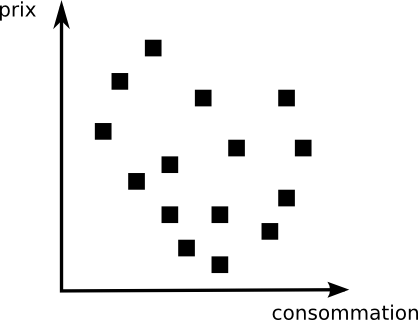
\includegraphics[width=.4\linewidth]{opti1.png}
  	}\qquad
    \subtop[\label{subfig_voiture:b}]{
	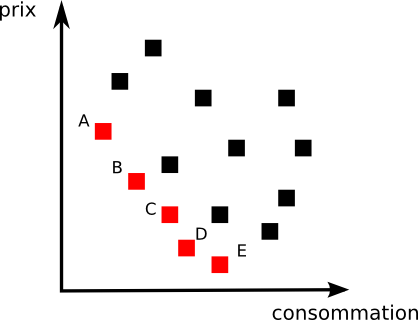
\includegraphics[width=.4\linewidth]{opti2.png}
  	}
    \subtop[\label{subfig_voiture:c}]{
  	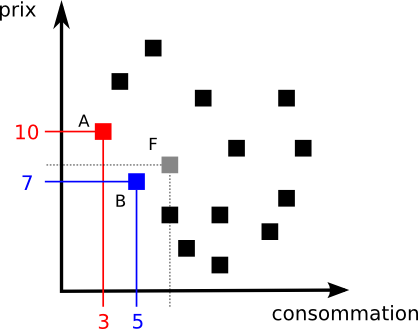
\includegraphics[width=.4\linewidth]{opti3.png}
  	}
 \end{sidecaption}
\end{figure}

\sloppy En regardant en détail les capacités des voitures figurant dans ce front \ref{subfig_voiture:c}, on voit bien que chacune d'entre elle domine une partie des autres voitures sur au moins un des deux objectifs. Si on prend le cas de la voiture F, celle-ci n'est pas prise en compte dans les solutions optimums, car le point est dominé sur ses deux objectifs par d'autres voitures : $ prix(B) < prix(F) < prix(A) $ et $consommation(A) < consommation (B) < consommation(F)$.

Le front de Pareto renvoie un ensemble de solutions compromis optimal, l'expertise finale sur la ou les solutions à adopter est donc le résultat d'un choix expert externe introduit comme support à l'algorithme optimiseur. Dans notre exemple, l'acheteur devra pour finaliser son achat mettre en avant au moins un des deux critères afin de départager les voitures.

Si certains algorithmes ont introduit cette expertise par le biais d'une sélection interactive guidant l'optimiseur à chaque étape de sa recherche, ce n'est pas cet usage qui nous intéresse ici. L'expertise n'intervient qu'une fois l'ensemble des solutions sélectionnées par l'optimiseur stabilisés, dans l'observation experte des résultats finaux.

Dans notre cas, on considère que l'optimiseur doit sélectionner avec les moyens qu'on lui a fournis les solutions candidates sur lesquels il doit miser pour converger. Il doit donc être capable de séparer les solutions en appliquant un ou plusieurs critères de séparation. Il existe plusieurs types de stratégies (\textit{Agreggation based, Criterion based, Dominance based, Indicator based}), et chacune d'elle peut être croisée ou dérivée en de multiples variantes \autocites[28]{Zitzler1999a, Deb2001}[7]{Liefooghe2009}. Nous limiterons ici notre analyse à un seul de ces cas, en nous focalisant d'ores et déjà sur les méthodes les plus utilisées en EC, basées sur la dominance celles-ci sont directement inspirées des travaux de Pareto.

% TODO : Finir ce paragraphe historique rapide, qui permettra de faire la différence ensuite avec les algorithmes inspirés par Pareto.
% TODO : Ajouter ref de Goldberg sur les sciences humaines + GA dans le chapitre 1

% \begin{figure}[!htbp]
% 	\begin{sidecaption}[fortoc]{Graphique en deux dimensions des fonctions objectifs $f_1$ et $f_2$ du tableau \ref{tab:pranking}}[fig:objf]
% 		\centering
% 		
\includegraphics[width=.4\linewidth]{pareto_ranking_a.pdf}
% 	 \end{sidecaption}
% \end{figure}


% \parbox{\marginparwidth}{
% \begin{enumerate}[label=(\alph*),labelindent=0pt,leftmargin=*]
%       \item $v_1$ est une \textit{fitness} calculée sur la base du nombre de dominé $+ 1$, cf. une partie de calcul de fitness de l'algorithme MOGA de \textcite{Fonseca1993}.
%       \item $v_2$ est une \textit{fitness} calculée sur la base du calcul de fronts de l'algorithme NDS de \textcite{Goldberg1989}. L'algorithme est assez simple, on fait comme si il s'agissait de peler un oignon. Au départ $r = 0$. On effectue un calcul de dominance sur une population complète $P$ (étape 1), puis on retire seulement les points non-dominés $P_{t+1} = P_{t} - P_{\varnothing}$ (étape 2) auxquels on attribue également un rang $r = r + 1$.  On recommence à l'étape 1 jusqu'à ce que tous les points possèdent un rang. Il existe également des variantes plus rapide de cet algorithme \autocite{Deb2001}.
% \end{enumerate}}

Pour comprendre comment cette stratégie opère et définir mathématiquement la notion d'optimum de Pareto, il faut introduire la notion de \textit{dominance} sur lequel elle s'appuie. Pour cette tâche on s'appuie sur les définitions données par \textcite[65]{Weise2011} :

\foreignblockquote{english}[{\cite[65]{Weise2011}}]{An element $x_1$ dominates (is preferred to) an element $x_2 (x_1 \dashv x_2)$ if $x_1$ is better than $x_2$ in at least one objective function and not worse with respect to all other objectives.}

Ce qui dans le cas d'une minimisation se traduit mathématiquement par les conditions suivantes :

% TODO : A CORRIGER ABSOLUMENT AVEC WEISE !!
\begin{align*}
	(x_1 \dashv x_2) \Leftrightarrow &\forall i \in 1 \dotsc n \Rightarrow  f_i (x_1) \leq f_i (x_2) \land \\
	&\exists j \in 1 \dotsc n : f_j (x_1) < f_j (x_2)
\end{align*}

Cette notion de \textit{domination} ($\succ$)\Anote{notation_dominance} permet de dégager ces trois possibilités

\begin{itemize}
\item $x_1$ domine $x_2$ , qui peut également s'écrire $x_1 \succ x_2$
\item $x_1$ est dominé par $x_2$
\item $x_1$ n'est pas comparable avec $x_2$
\end{itemize}

Celle-ci possède les propriétés suivantes, qui définissent dans l'espace des objectifs $\mathbb{Y}$ un \textit{strict partial order} :

\begin{enumerate}
\item{\textbf{non reflexive}}  $x_1$ ne peut pas se dominer lui même
\item{\textbf{non symétrique}} $ x_1 \succ x_2$ n'implique pas $x_2 \succ x_1$, alors que l'opposé est vrai, $x_1 \succ x_2$ implique $x_2$ ne domine pas $x_1$
\item{\textbf{transitive} }
\end{enumerate}



\begin{testiv}{Fitness et stochasticité dans les simulations}{}

L'effet de la stochasticité sur les dynamiques à l'oeuvre dans les modèles est un problème difficile à cerner, or celui-ci a un impact très fort sur les résultats d'une exploration lorsqu'on utilise des métaheuristiques. On va voir pourquoi dans cet encadré.

Une des solutions pour lisser les effets de la stochasticité est de réaliser un certain nombre de \textbf{réplications} dans l'exécution des simulations. Cette opération consiste à exécuter plusieurs fois une simulation à jeu de valeurs de paramètres identiques en ne faisant varier que la graine aléatoire, afin de mesurer le poids de l'aléa dans la variation des objectifs mesurés. Contrairement à ce que l'on pourrait penser, il n'y a pas de chiffre \enquote{magique} pour déterminer le nombre correct de réplications. Celui-ci peut varier en fonction de l'objectif mesuré, mais également en fonction des valeurs de paramètres utilisées. Seule une exploration plus systématique peut amener un début de réponse. La forme de la distribution obtenue a également peu de chance d'être une gaussienne, ce qui rend l'utilisation d'une moyenne pour résumer les résultats assez peu recommandé.

\begin{figure}[H]
		\centering
	 	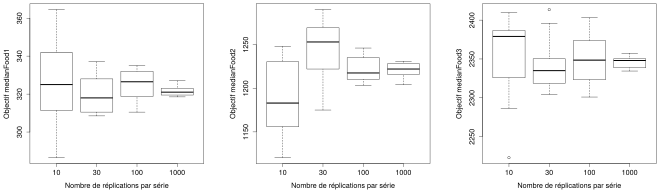
\includegraphics[width=1.0\linewidth]{ant_serie_stoch.pdf}
\end{figure}

Pour réaliser ce type de graphique, on réalise $10$ séries de $10$, de $30$, de $50$, de $100$ puis de $1000$ réplications pour un jeu de valeur de paramètres test fixé à $\{population = 125.0, diffusion-rate = 25.0, evaporation-rate = 25.0\}$. D'autres jeu de valeurs de paramètres donneraient probablement des résultats différents.

Dans le cas de l'exemple \textit{Ants}, on voit bien qu'en fonction du nombre de réplications, la valeur trouvée sur les objectifs ${medianFood1, medianFood2, medianFood3}$ est très variable. Si le nombre de réplications est trop faible, il est tout à fait possible que l'optimiseur sélectionne comme satisfaisantes des solutions candidates qui amènent le calcul d'une \textit{fitness} satisfaisante \enquote{une fois de temps en temps} ...

S'il n'est pas possible de réaliser le nombre de réplications idéales/suffisantes, ce qui est souvent le cas, alors il est conseillé de réévaluer régulièrement les solutions candidates retenues par l'optimiseur. C'est particulièrement important dans le cas des Algorithmes Evolutionnaires mobilisant une population de solutions candidates, car ceux-ci conservent et remobilisent les meilleurs individus entre les différentes itérations. Une fois entré dans cette population \enquote{par chance}, l'individu va continuer à fournir une descendance dont les capacités estimées sont biaisées.

Ce cas a été rencontré lors des expérimentations pour SimpopLocal. Ce modèle de simulation nécessite en effet l'exécution d'au moins $100$ réplications si on veut lisser correctement les erreurs sur les différents objectifs. Devant le nombre d'évaluations du modèle réalisé (plusieurs millions), seul $30$ réplications ont pu être faites pour chaque jeu de valeurs de paramètres. Un mécanisme spécifique à été intégré à MGO pour permettre la réévaluation aléatoire des meilleures solutions conservées par l'optimiseur (Algorithme Evolutionnaire) \autocite[193]{Schmitt2014}.

\end{testiv}


Différents degrés de dominance ont été développés, comme par exemple la notion de \textit{strong dominance} : $x_1$ domine fortement $x_2$ ($x_1 \succ \succ x_2$) si $x_1$ est strictement meilleur que $x_2$ sur tout ses objectifs.

\begin{table}[!h]
	\centering
	\begin{sidecaption}[Règle de dominance pour les points e et f]{Application des règles de dominance aux points $e$ et $f$. \\ \\
		   \begin{tabular}{>{$}l<{$}>{$}l<{$} >{$}l<{$}}
					\toprule
					 & f1 & f2 \\
					\midrule
					e      & 0.5    &  4   \\
					f      & 0.5    & 5,5  \\
					\bottomrule
			\end{tabular}\\ \\
			(a) $e \succ f$ car e est bien le meilleur sur au moins un des deux objectifs, et n'est pas pire sur aucuns des autres objectifs ($e \succeq f$ ) \\
			(b) f ne domine pas e car f n'est pas meilleur sur aucun des deux objectifs et il est pire sur au moins un des deux objectif}[tab:minipranking]

		\begin{minipage}{0.5\textwidth}
			\centering
			\subbottom[e est dominé par f ?\label{pranking_a}]{
				\begin{tabular}{>{$}l<{$}>{$}l<{$} >{$}l<{$}}
					\toprule
					    & f1 & f2 \\
					\midrule
					e \leq f & \text{true} & \text{true} \\
					e < f   & \text{false}  & \text{true} \\
					\bottomrule
				\end{tabular}
		 	}
		 \end{minipage}\hspace{1em}
		 \begin{minipage}{0.5\textwidth}
		 	\centering
			\subbottom[f est dominé par e ?\label{pranking_b}]{
				\begin{tabular}{>{$}l<{$}>{$}l<{$} >{$}l<{$}}
					\toprule
					  & f1 & f2 \\
					\midrule
					f \leq  e & \text{true} & \text{false} \\
					f < e  & \text{false}  & \text{false} \\
					\bottomrule
				\end{tabular}
			}
		\end{minipage}
  \end{sidecaption}
\end{table}

Pour bien comprendre comment se construit l'ensemble $X^*$ de solutions non dominées $x^* \in \mathbb{X}$ ,on peut étudier en détail dans le tableau \ref{tab:minipranking} comment la dominance se calcule entre les points $e$ et $f$, toujours tirés du tableau \ref{tab:pranking}.

Les solutions admises parmi le front de Pareto (voir figure \ref{fig:frontoptimal}) sont donc ici toutes celles qui ne sont pas dominées faiblement ($\succeq$), ce qui revient à exclure les points $f$ et $l$ du front optimum $\{a,b,c,d,e\}$ car ils sont dominés faiblement ($e \succeq f$); alors que dans le cadre d'une dominance forte ($\succ \succ$), ceux-ci auraient fait partie du front $\{a,b,c,d,e,f,l\}$. En effet si on prend toujours le cas de $e$ et $f$, la condition testant que $e$ est strictement meilleur que $f$ sur tous les objectifs n'est pas remplie.

%Cet ensemble de cardinalité forcément inférieure ou égale est qualifié \enquote{d'ensemble fort non dominé} (\textit{Strongly non dominated set}).

Le front de Pareto pour $\succ \succ$ est plus \textbf{grand} que le front de Pareto pour $ \succ $. Or $\succ \succ$ est \textbf{plus stricte} que $\succ$. Le raisonnement est contre-intuitif, par conséquent nous allons le dérouler plus en détail par la suite en observant de plus près le cas litigieux, c'est-à-dire pour le point $f$ et $l$, car $f_1 = e_1$

\pagebreak

On examine si $f$ doit être exclu de l'ensemble Front de Pareto $FP$ dans les deux cas, pour une dominance forte ($\succ \succ$) et une dominance faible ($\succeq$)

\medskip

\textbf{1) Dans le cas d'une dominance forte : }
\begin{align*}
     si f \notin FP & \Rightarrow \exists x \in FP \\
     & \text{tel que }  x \succ \succ f
\end{align*}

On teste tous les éléments de $FP$, le seul qui pose question est le point $e$, on pose donc la question suivante, est ce que $e \succ \succ f$ ?

\textbf{Non,} car $f_1(e) = f_1(f)$ , et donc $e$ ne domine pas fortement $f$. N'étant pas en mesure d'établir un ordre entre ces valeurs, il est impossible d'exclure $f$ de $FP$, et donc $ f \in FP_{\succ \succ}$

\medskip

\textbf{2) Dans le cas d'une dominance faible : }
On reprend la définition qui nous est donné, $ e \succeq f$ si
\begin{enumerate}[label=(\arabic*),labelindent=\parindent,leftmargin=*]
\item $ \forall_i \ e_i \leq f_i$
\item $ \exists_j \ e_j < f_j$
\end{enumerate}

\medskip

Or (1) est bien $True$ d'après le tableau \ref{pranking_a}, il est donc possible d'écrire $e_1 \leq f_1$ et $e_2 \leq f_2$. Le cas (2) est également $True$ car $e_2 < f_2$

\medskip

\textbf{Par conséquent}, le fait que (1) et (2) soit égal à $True$ permet, à la différence de la dominance forte, de discriminer $e$ par rapport à $f$, ce qui fait  que $e_2 \succeq f_2$. Donc $f \notin FP_{\succeq}$

\begin{table}[!p]

\begin{sidecaption}[Tableau résumé des fonctions objectifs, et de différentes valeurs de fitness associées]{Tableau de résultats des fonctions objectifs $f_1$ et $f_2$ pour un vecteur de solutions candidates $\{a \dotsc p\}$ dans l'espace des objectifs $\mathbb{Y}$, et résultat du \textit{Pareto Ranking}, intervenant ensuite dans le calcul de \textit{fitness} de différentes façons selon les algorithmes utilisés.}
	[tab:pranking]
	\centering
	 \subbottom[Graphique en deux dimensions des fonctions objectifs $f_1$ et $f_2$ du tableau ci-dessous.\label{pranking:a}]{
  		
\includegraphics[width=.4\linewidth]{pareto_ranking_a.pdf}
  	}\qquad
	\subbottom[Tableau de données pour les solutions candidates des différents exemples.\label{pranking:b}]{
	\begin{threeparttable}
	\begin{tabular}{>{$}l<{$} >{$}l<{$} >{$}l<{$} >{$}l<{$} >{$}l<{$} >{$}l<{$}}
			\toprule
			\text{solutions candidates} & f_1 & f_2 & \text{dominé par} & v_1\tnote{1} & v_2\tnote{2} \\
			\midrule
			a      & 3.5    & 1    &  \varnothing & 1 & 1 \\
			b      & 3      & 1,5  &  \varnothing & 1 & 1 \\
			c      & 2      & 2    &  \varnothing & 1 & 1 \\
			d      & 1      & 3    &  \varnothing & 1 & 1 \\
			e      & 0.5    & 4    &  \varnothing & 1 & 1 \\
			f      & 0.5    & 4.5  &  \{e \}      & 2 & 2 \\
			g      & 1.5    & 4.5  &  \{d,e,f,h \} & 5 & 3 \\
			h      & 1.5    & 3.5  &  \{d \}      & 2 & 2 \\
			i      & 2      & 3.5  &  \{c,d,h \}  & 4 & 3 \\
			j      & 2.5    & 3    &  \{c,d \}    & 3 & 2 \\
			k      & 3.5    & 2    &  \{a,b,c \}  & 4 & 2 \\
			l      & 4.5    & 1    &  \{a \}      & 2 & 2 \\
			m      & 4.5    & 2.5  &  \{a,b,c,k,l \} & 6 & 3 \\
			n      & 4      & 4    &  \{a,b,c,d,e,h,i,j,k,o \} & 11 & 5 \\
			o      & 3      & 4    &  \{b,c,d,e,h,i,j \} & 8 & 4 \\
			p      & 5     & 4.5   &  \{a,b,c,d,e,f,g,h,i,j,k,l,m,n,o \} & 16 & 6 \\
			\bottomrule
	\end{tabular}
	\begin{tablenotes}
      \small
      \item[1] $v_1$ est une \textit{fitness} calculée sur la base du nombre de dominé $+ 1$, cf. une partie de calcul de fitness de l'algorithme MOGA de \textcite{Fonseca1993}.
      \item[2] $v_2$ est une \textit{fitness} calculée sur la base du calcul de fronts de l'algorithme NDS de \textcite{Goldberg1989}. L'algorithme est assez simple, on fait comme s'il s'agissait de peler un oignon. Au départ $r = 0$. On effectue un calcul de dominance sur une population complète $P$ (étape 1), puis on retire seulement les points non-dominés $P_{t+1} = P_{t} - P_{\{\varnothing\}}$ (étape 2) auxquels on attribue également un rang $r = r + 1$.  On recommence à l'étape 1 jusqu'à ce que tous les points possèdent un rang. Il existe également des variantes plus rapide de cet algorithme \autocite{Deb2001}.
    \end{tablenotes}
	\end{threeparttable}}
  \end{sidecaption}
\end{table}

\pagebreak

\begin{figure}[!htb]
	\begin{sidecaption}[Tracé d'un front de Pareto]{Tracé du front optimum à partir du calcul des individus non dominés, cf. l'ensemble vide $\varnothing$ dans le tableau \ref{tab:pranking}}[fig:frontoptimal]
		\centering
		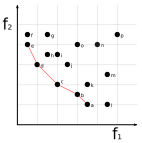
\includegraphics[width=.4\linewidth]{pareto_front.pdf}{
		}
  \end{sidecaption}
\end{figure}

Le front de Pareto n'est en général jamais entièrement couvert, cela pour diverses raisons :

\begin{itemize}
\item L'évaluation de la fonction à optimiser est souvent coûteuse, comme dans le cas de modèle de simulation dont l'exécution peut prendre jusqu'à plusieurs dizaines de minutes,
\item La zone d'exploration est volontairement bornée du fait des objectifs des expérimentateurs,
\item La stochasticité oblige l'exécution de nombreuses réplications d'une même évaluation,
\item On dispose de ressources finies, or l'espace du front est souvent continu et non borné en dehors des contraintes que l'on aura nous-mêmes fixées.
\end{itemize}

Selon \textcite[70]{Weise2011} et \textcite[19]{Zitzler1999a}, on peut s'aider dans cette tâche d'établissement d'un front de Pareto correct en étant attentif aux points suivants:

\begin{enumerate}
\item{\textbf{Proximité}} Les solutions découvertes doivent être les plus proches possibles du front de Pareto optimal.
\item{\textbf{Diversité}} Si le front optimal possible est trop large, la répartition des solutions \textit{spread} doit être maximisé sur toute la surface de celui-ci, si possible suivant une distribution uniforme.
\item{\textbf{Pertinence}} Les solutions découvertes doivent correspondre aux intérêts définis par le problème, et n'ont aucun intérêt si l'opérateur humain ne peut, ou ne sait les utiliser.
\end{enumerate}

On retrouve dans ces objectifs la tension entre exploration et exploitation, le front de Pareto devant être exploité de façon homogène, tout en garantissant à terme (et si possible le plus vite possible) la convergence vers une zone d'intérêt pour l'expérimentateur (voir figure \ref{fig:convergence_diversite}). Les métaheuristiques n'ayant pas d'apriori sur la forme de problème abordée, c'est dans l'originalité, la diversité des constructions proposées qu'une solution optimale et dédiée peut être trouvée. Il est donc très difficile de faire un listing des meilleures stratégies, et des meilleures combinaisons de stratégies permettant une sélection garantie des meilleurs candidats en fonction de ces objectifs, l'établissement de cette liste ne pouvant être que contextuelle d'un problème d'optimisation donné\Anote{no_free_lunch}.

Heureusement, un certain nombre de combinaisons, souvent éprouvées par de multiple tests sur des fonctions aux caractéristiques et difficultés soigneusement étudiées (ZDT, etc.), se démarquent par des capacités de résolution acceptable. C'est d'ailleurs souvent sur cette première base que se construisent ensuite les améliorations nécessaires à une réponse optimale, cela en partie grâce à la flexibilité des composantes caractéristique des métaheuristiques.

\begin{figure}[!htbp]
  \begin{sidecaption}[Comparaison entre deux fronts de Pareto, avec et sans maintien de la diversité]{Convergence et maintien de la diversité au sein du front de Pareto}[fig:convergence_diversite]
  \centering
  \subbottom[Un front de pareto sans maintien suffisant de la diversité.\label{subfig_convergence_diversite:a}]{
  	\includegraphics[width=.4\linewidth]{pareto_convergence_a.pdf}
  	}\qquad
  \subbottom[Un front de pareto avec maintien de la diversité.\label{subfig_convergence_diversite:b}]{
	\includegraphics[width=.4\linewidth]{pareto_convergence_b.pdf}
  	}
 \end{sidecaption}
\end{figure}

\textit{Une fois défini cet ordre partiel entre les solutions candidates évaluées, sur quelle base l'optimiseur prend sa décision pour sélectionner les individus les plus prometteurs ? et comment celui-ci garantit l'évolution des solutions candidates selectionnées au regard des trois objectifs fixés ?}

Comme le dit de façon très claire,\textcite[94]{Weise2011} \foreignquote{english}{Such comparisons, however, only state whether one candidate solution is better than another one or not, but give no information on \textbf{how much} it is better or worse and \textbf{how interesting} it is for further investigation. Often, such a scalar, relative measure is needed.}

L'optimiseur n'ayant pas les capacités pour comparer des fonctions entre elles, c'est par l'attribution d'un scalarlaire caractérisant chaque vecteur $z^* \in \mathbb{Y}$ résultat de l'évaluation d'une solution candidate, que celles-ci vont pouvoir être départagées. On parle de \enquote{fonction d'utilité}, ou de \enquote{fonction \textit{fitness}} pour désigner cette opération de transformation dont le résultat $z$ est utile uniquement en se plaçant dans le référentiel de l'optimiseur. Il s'agit d'un classement relatif des solutions les unes par rapport aux autres, calculés indépendamment des valeurs prises par les fonctions objectives, et intégrant un certain nombre d'autres critères, définis en réponse aux exigences des trois objectifs déjà évoqués (respect de la diversité, qualité de convergence, pertinence vis-à-vis du problème).

Ainsi, un des tout premiers paramètres à intégrer dans le calcul de cette fonction \textit{fitness} tient évidemment dans le choix d'une stratégie adaptée pour tirer le meilleur parti des informations récoltées dans l'application de cet ordre partiel sur l'espace $\mathbb{Y}$. Là ou des algorithmes vont appuyer la sélection des solutions à partir d'un calcul de rang (je ne garde que les $n$ premiers rangs), d'autres vont le faire à partir d'un décompte des non dominés (je ne garde que les individus non dominés $< n$), à partir d'une profondeur (je ne garde que les $n$ premiers fronts), ou encore en mélangeant ces différentes informations (voir les calculs effectués dans le tableau \ref{tab:pranking}) A cela il faut également ajouter la diversité de choix à disposition dans la selection d'une dominance, par le changement de l'opérateur utilisé dans le calcul (\textit{weak dominance}, \textit{strong dominance}, etc.), ou même la relaxe de celui-ci (\textit{epsilon-dominance}). Des choix de première importance, car ils interviennent directement dans la construction de l'ensemble de solutions retenues.

%\pagebreak

\bigskip

\begin{testiv}{L'epsilon dominance par l'exemple}{}

Soit deux fonctions objectifs $f_1$ et $f_2$, et une population de $10$ solutions candidates parmi lesquels l'optimiseur ne peux choisir que les $5$ meilleurs valeurs pour formuler les prochaines solutions candidates à évaluer. Une fois triés par ordre descendant sur les deux objectifs, on vient bien que l'optimiseur s'est focalisé autour de $[25.00, 25.05]$.

\begin{figure}[H]
	 \centering
	 	\includegraphics[width=0.8\linewidth]{epsilon_dominance.pdf}
	 	\label{fig:epsilon}
\end{figure}

La diversité à ce niveau de résolution doit paraître suffisante à l'optimiseur pour qu'il continue à sélectionner des candidats proches de $25$. Mais le gain est minime et cette pression sur $f_{2}$ masque peut être l'existence de meilleur compromis ailleurs.

\begin{table}[H]
	\centering
		\begin{minipage}{0.5\textwidth}
			\centering
			\subbottom[Valeurs triés pour $f_{1}$ et $f_{2}$ \label{epsilon_a}]{
			\resizebox{0.6\textwidth}{!}{%
				\begin{tabular}{@{}lll@{}}
				\toprule
				 & $f_{1}$ & $f_{2}$ \\ \midrule
				 1 & 9 & 25.00993 \\
				 2 & 9 & 25.01002 \\
				 3 & 10 & 25.01012 \\
				 4 & 10 & 25.01041 \\
				 5 & 11 & 25.01056 \\
				6 & 19 & 25.05121 \\
				7 & 20 & 16.3084 \\
				8 & 24 & 18.1433 \\
				9 & 26 & 18.2331 \\
				10 & 30 & 45.3212 \\ \bottomrule
				\end{tabular}%
		 }
		 }
		 \end{minipage}\hspace{0.2em}
		 \begin{minipage}{0.6\textwidth}
			\centering
			\subbottom[Mise en place d'un epsilon de $0.5$ \label{epsilon_b}]{
			\includegraphics[width=0.8\linewidth]{epsilon_dominance_avec.pdf}
			}
		\end{minipage}
\end{table}

Une des possibilités est donc d'utiliser un epsilon de $0.05$ indiquant à l'optimiseur, au moment du calcul de la dominance, de considérer comme équivalentes les solutions dans ce radius autour d'un individu. Cela revient à relâcher la pression sur un des objectifs pour permettre à l'autre de s'exprimer. Dans notre exemple les $5$ premières solutions seront alors considérées comme équivalentes par l'optimiseur, et celui-ci se focalisera donc moins sur les micro-gains possibles sur $f_{2}$ au profit d'une plus grande diversité sur $f_{1}$. 

Une \textit{epsilon-dominance} a également été utilisée pour SimpopLocal, car un des objectif (population) était beaucoup trop sensible (voir annexe \ref{sec:simpoplocal}).

\end{testiv}

C'est donc dans l'espace des objectifs $\mathbb{Y}$ que se révèle la première information pertinente pour l'optimiseur, nous indiquant, peu importe la forme de l'une ou de l'autre des fonctions et le positionnement des points sur celles-ci, une première sélection de solutions parmi les solutions candidates évaluées sur laquelle l'effort de l'optimiseur doit porter en priorité.

Mais lorsque l'on reprojette les résultats du front de Pareto dans l'espace figurant la dynamique supposée de chacune des deux fonctions objectifs, on observe que la prise de décision basée sur le seul ordonnancement des solutions n'est pas suffisante pour garantir une selection optimale des meilleurs candidats à l'évolution (voir figure \ref{fig:mo_landscape}).

La forme des fonctions dans cette figure est représentée en pointillé car elle n'est qu'une description temporaire d'un paysage en partie inconnu, en attente d'être révisée par l'évaluation de nouveaux points. Le tracé d'un paysage ne se confond plus comme cela pouvait être le cas dans une optimisation mono-objectif avec la valeur prise par la fonction objectif, et doit maintenant intégrer un intermédiaire supplémentaire plus complexe qui est le calcul d'une fonction \textit{fitness}, et dont la formulation, dépendante de nombreuses stratégies, va modifier les solutions choisies dans le futur, et donc modifier la façon dont on va découvrir l'approximation de ce paysage, cela de façon indépendante aux objectifs choisis. \autocite{Weise2011}

\begin{figure}[!htbp]
	\begin{sidecaption}[Projection des individus extraits du front de Pareto dans l'espace des paramètres]{Projection du front de Pareto optimal (point \sqbox{tangoBlack1}), et des autres solutions candidates dominées (point \sqbox{tangoGrey1}) sur l'espace de variation du paramètre $x \in \mathbb{R}$, un schéma inspiré par \textcite[67]{Weise2011}
	\parbox{\marginparwidth}{
	\begin{enumerate}[label={},labelindent=0pt,leftmargin=*]
	      \item \sqbox{tangoBlue1} $f_{1}(x)$
	      \item \sqbox{tangoRed1} $f_{2}(x)$
	\end{enumerate}}\\
	Les fonctions $f_{1}(x)$ et $f_{2}(x)$ sont représentées en pointillé car elles sont inconnues de l'optimiseur, et ne servent que de repère au lecteur pour mieux comprendre comment un paysage caractérisant l'intersection des deux fonctions peut émerger durant l'optimisation, et pourquoi cela peut être intéressant d'intégrer son analyse à l'optimiseur.}[fig:mo_landscape]
	 \centering
	 	\includegraphics[width=0.8\linewidth]{multi_objective_landscape.pdf}
	\end{sidecaption}
\end{figure}

%on se rend également compte qu'un surplus d'information tiré de l'exploitation d'autres espaces pourrait être utile au choix de l'optimiseur

%\Anote{weise_multi2D}
Déjà beaucoup plus difficile à imaginer que dans l'exemple précédent de l'équation de Schaeffer, la re-projection des solutions candidates évaluées se fait sur un nouvel espace $\mathbb{G}$ (voir figure \ref{fig:relation_espaces}), qui inclut l'ensemble de tout les éléments $g \in \mathbb{G}$ pouvant être manipulés par les opérateurs de recherche à disposition de l'optimiseur \autocite[82]{Weise2011}. Un processus détaillé un peu plus tard dans cette section.

Dans notre cas $x \in \mathbb{R}$, on a donc un paramètre qui est manipulable et peut prendre une infinité de valeurs dans le cadre des contraintes définies pour $x$ (par exemple une valeur de 0 à 10 pour $x$)\Anote{remarque_resolution}. L'espace $\mathbb{G}$ contient la codification du problème, ce qui par exemple dans le cadre de simulation, se traduit pour chaque élément $g$ par l'attribution d'un vecteur de paramètres définissant les entrées de la simulation sur lequel l'optimiseur va pouvoir \enquote{jouer} pour optimiser les différentes fonctions objectifs.

La fonction $gpm : \mathbb{G} \to \mathbb{X}$ est une translation opérée lorsque les deux espaces sont de nature différente, par exemple pour passer d'un espace Binaire à un espace de Réels $\mathbb{B} \to \mathbb{R}$. Dans le cadre de simulations, les deux espaces sont souvent de nature similaire $\mathbb{G} = \mathbb{R}$. On pourra se référer à \textcite[86-88]{Weise2011} pour plus de détails.

\begin{figure}[!htbp]
	\begin{sidecaption}[Résumé des relations entres les différents espaces d'une optimisation]{Résumé des relations entre les différents espaces dans une optimisation}[fig:relation_espaces]
		\centering
		\includegraphics[width=.7\linewidth]{objectifsToSearchSpace.pdf}
  \end{sidecaption}
\end{figure}

%D'une part, l'observation de dynamiques en partie contraires sur ces deux fonctions $f_1$ et $f_2$ nous permet de constater encore une fois pourquoi un déplacement de l'optimiseur sur l'une ou l'autre des fonctions dirigé par la recherche d'un optimum n'a aucun sens.

L'opération de sélection des solutions candidates est souvent rattachée au processus de convergence. L'objectif de l'optimiseur est d'évaluer au mieux le potentiel de chacune des solutions durant cette phase de sélection pour intégrer et conserver les meilleurs éléments à son référentiel entre deux itérations. On imagine pourtant très bien l'effet que peut avoir une sélection trop restrictive sur le maintien de la diversité. C'est le cas par exemple si l'optimiseur ne décide de garder que le front de Pareto, on voit bien sur la figure \ref{fig:mo_landscape} à quel point la couverture de la dynamique des deux fonctions ressortirait considérablement appauvrie à la suite d'un tel choix. On en déduit que la frontière entre stratégies de convergence, et stratégies de maintien de la diversité doit être assez perméable pour garantir le choix de solutions candidates pertinentes en dehors du seul front de Pareto. \textcite{Zitzler1999a} retient par exemple parmi ces classes de stratégies celle s'appuyant sur le couple associant espace des objectifs et au choix la dominance, la densité, le temps, ou encore la chance. Ce sont des heuristiques qui vont intervenir en amont sur la qualité et la diversité des solutions candidates (par exemple les stratégies de \textit{sharing}, \textit{crowding}, etc.) qui peuvent ensuite être manipulées par les opérateurs de recherches de l'optimiseur.

Viennent ensuite les stratégies de recombinaison des solutions selectionnées, créatrices de nouvelles solutions candidates à évaluer. Un processus qui peut être là aussi rattaché tout autant au maintien de la diversité qu'à une volonté de convergence accrue. Il n'y a là encore aucune règle d'applications spécifiques, et tout dépend de l'objectif fixé de façon initiale ou au cours de l'expérimentation. Ainsi, certaines stratégies intégrées aux opérateurs peuvent être mis en place pour limiter une convergence trop rapide des solutions (\textit{premature convergence} généralement associé à une perte de diversité), alors que d'autres vont tenter d'accélérer cette convergence par la mise en oeuvre d'opérateur de recherche plus agressif, soit pour trouver le plus rapidement possible un minimum (ou maximum) local, soit car la topologie de l'espace des objectifs est difficile.

La sélection de candidats à la manipulation dans l'espace des objectifs $\mathbb{X}$ se réfère, une fois projetée dans cet espace $\mathbb{G}$, aux éléments $g$ accessibles à la manipulation par les opérateurs de recherche de la fonction $searchOp$. Chacun de ces opérateurs, dont le nombre et la nature est un paramètre de l'optimiseur, s'appuie sur la transformation d'une ou plusieurs solutions candidates dirigée par la création d'un nouvel élément $g$, dont on attend si possible un meilleur résultat à l'itération suivante. Un postulat très fort est posé par ce type de méthodes d'optimisation, l'introduction de petites variations sur les valeurs de l'espace de recherche est également censée apporter de petites variations dans l'espace des objectifs, que cela résulte en une amélioration ou en une dégradation de la qualité. Appelée \textit{strong causality}\Anote{note_strong}, cette propriété est évidemment dépendante de la forme prise par le paysage du problème (\textit{problem landscape}), et plus celui-ci est accidenté, rugueux, plus sa résolution est considérée comme complexe\Anote{note_weak}.

En relation avec cette observation, l'éclatement de cette population de solutions candidates évaluées sur le paysage nous permet de constater (voir la figure \ref{fig:mo_landscape}) à quel point la notion de distance entre les points paraît différente entre ces deux espaces. $f$ et $c$ apparaissent ici beaucoup plus proches d'un optimum global que $a$ et $b$, ces deux derniers étant pourtant plus proches de $c$ que $f$ dans l'espace des objectifs. On voit bien ici que la sélection de solutions candidates intéressantes peut intégrer d'autres informations utiles, en supplément de celles fournies par l'analyse de $\mathbb{Y}$, au travers de l'analyse de cet espace $\mathbb{G}$; et cela toujours afin de guider au mieux l'optimiseur dans la sélection des candidats à l'évolution. Un croisement du positionnement des individus $f$ et $c$ donnerait ainsi une bien meilleure valeur de $x$ à évaluer, probablement meilleure que celle d'un individu $a$ et $c$. Si la solution $f$ avait été éliminée sur le fait d'une sélection aux critères plus drastiques, c'est aussi la possibilité d'un croisement fructueux avec $c$ qui disparaît.

%A ces stratégies principales s'ajoute un autre ensembles de stratégies, dont certaines sont plus spécifiques, ou constitutives des types d'algorithmes utilisés. %Le maintien d'une diversité de solutions entre les itérations fait partie de ces stratégies qui font partie d'un set plus large de stratégies permettant de contrer l'émergence des différentes difficultés (stochasticité, topologie, etc.) caractéristique d'un problème de résolution unique.

%Généralement nommé \foreignquote{english}{Pareto Ranking}\Anote{utilisation_pareto_ranking} aussi nommé par Weise \foreignquote{english}{Prevalence Ranking}.

%\pagebreak
\bigskip

\begin{testiv}{De l'espace de paramètre à l'espace des objectifs sur l'exemple Ants}{}

\begin{center}
	 	\includegraphics[width=0.6\linewidth]{matrix.pdf}
\end{center}

Un algorithme évolutionnaire a été utilisé pour trouver quels étaient les valeurs minimales de valeurs objectifs atteignables avec le modèle \textbf{Ants}. Autrement dit, on demande à l'algorithme d'optimisation de nous dire, dans la mesure du possible, quels sont les valeurs de paramètres (génome) nous permettant de minimiser au mieux la durée (trois fonctions objectifs ${f1,f2,f3}$) pour consommer le tas de nourriture 1, 2 et 3. Au bout d'un certain nombre d'itérations, cet algorithme nous propose un ensemble de solutions résultats incluant le front de Pareto, constitué ici de 3 dimension. Une vidéo de l'optimisation, les données au format csv, et le \textit{workflow} ayant permis d'arriver à ces résultats sont accessibles sur le site compagnon de la thèse (voir notes de lecture).

Comme il n'existe pas d'outil facile d'emploi permettant de sélectionner des points dans un espace en 3 dimensions tout en affichant simultanément les valeurs de paramètres auxquelles chacun de ces points est rattaché, nous allons nous contenter d'un autre outil en deux dimensions. Connu sous le nom de \textit{scatterplot matrix}, celui-ci permet de représenter un ensemble de points présents sous forme tabulaire classique vers la forme de matrice, comme représenté dans la figure ci-dessus.

Dans une forme interactive de cette représentation\Anote{scattrplot}, la sélection à la souris d'un ensemble de points met automatiquement en lumière la position de ceux-ci dans l'ensemble de la matrice. Dans notre cas, à chaque point sont associées les valeurs de paramètres suivantes $(diffusion-rate,evaporation-rate, medianFood1, medianFood2, medianFood3)$ Cette représentation permet d'explorer la relation entre l'espace des objectifs et l'espace des valeurs de paramètres en mettant tout sur le même plan 2D. Cette exercice d'analyse, encore faisable en deux dimensions, devient un peu plus difficile à réaliser à chaque fois que l'on ajoute des paramètres ou des objectifs. Afin de ne pas encombrer ce chapitre par des dizaines de matrices, j'ai choisi de réunir dans un seul et même schéma les différentes sélections (voir la zone encadrée de pointillé rouge dans la matrice) en prenant pour axe $x$ de référence l'objectif $f3$ minimisant la durée pour épuiser le tas de nourriture 3 le plus éloigné du nid.

\begin{center}
	\includegraphics[width=0.9\linewidth]{resume.jpg}
\end{center}

Il ne faut pas oublier que cette analyse se fait sur une population de solutions évaluées stabilisée, elle est donc très resserrée autour de certains comportements clefs. Des frontières qui renseignent le modélisateur sur les contradictions auxquelles l'algorithme d'optimisation doit faire face pour minimiser ces trois objectifs à la fois. On voit bien que les écarts sont très différents selon les objectifs, ce qui peut parfois poser problème à l'optimiseur.

\begin{itemize}[nolistsep]
	\item Dans la colonne (a), on s'intéresse à un premier cluster de valeurs d'évaporation compris entre $[5.5, 10]$. On voit que pour cette sélection le taux de diffusion est très étalé, entre $[20, 80]$, ce qui indique le peu d'impact de celui-ci dans cette dynamique. Quelque soit la valeur dans cet intervalle, le modèle est toujours proche de valeurs égale à $800$ à +/- $100$ près pour \textit{medianFood3}. S'il y a bien une forme de stabilité exprimée pour ce troisième objectif, le deuxième objectif est par contre beaucoup plus sensible car sa valeur peut varier entre $[300, 550]$. De la même façon, la valeur de l'objectif \textit{medianFood1} est très étalée entre $205$ et $230$. On pourrait qualifier de comportement moyen ce profil, car il ne donne pas les pires résultats sur l'objectif \textit{medianFood3}, il donne des résultats assez resserrés entre $[200, 230]$ sur l'objectif \textit{medianFood1}. Pour l'objectif \textit{medianFood2} par contre, c'est moins clair, il semble y'avoir un effet de seuil.
	\item On sélectionne un cluster qui partage certaines valeurs avec le précédent, sur les valeurs d'évaporations comprises entre $[5, 6]$. On voit qu'avec ces valeurs-là, il est possible d'atteindre des valeurs minimales sur l'objectif \textit{medianFood3}, aux environs de $600$. La lecture de $diffusion-rate$ nous indique qu'il faut se concentrer sur des valeurs comprises entre $[15, 40]$ pour observer cet effet. Des valeurs qui se chevauchent avec la tranche donnée précédemment dans la colonne (a), entre $[20, 60]$. Il faut que ces deux conditions réunies (taux d'évaporation $< 6$ et taux de diffusion compris entre $[20, 40]$) pour qu'une valeur minimale puisse etre atteinte sur l'objectif \textit{medianFood3}. Dans cette configuration, les résultats sur l'objectif \textit{medianFood1} sont moins bons que précédemment, l'optimiseur a du faire un compromis. La valeur sur l'objectif \textit{medianFood2} est stable autour de $400$, alors dans la colonne (a) ce n'était pas le cas. Le point de tension semble donc plus être entre l'objectif \textit{medianFood1} et \textit{medianFood3}, ce qui semble assez logique vu la configuration des tas de nourriture 1 et 3. Il faut toutefois aussi relativiser la dégradation des performances sur cet objectif \textit{medianFood1}, elles sont minimes entre (a) et (b) (entre $0$ et $50$ d'écart max avec (a)), surtout en comparaison du gain obtenu sur l'objectif \textit{medianFood2}, devenu plus stable, et \textit{medianFood3} moins long de $200$ vis à vis de (a). Cette configuration de paramètres paraît etre la plus intéressante pour le moment, tout dépend de l'importance accordée par le modélisateur à la dégradation de performance sur l'ojectif \textit{medianFood1}.
	\item La colonne (c) montre de toute évidence que les candidats les meilleurs sur l'objectif \textit{medianFood1} $< 200$, sont aussi potentiellement les plus mauvais sur l'objectif \textit{medianFood2} et \textit{medianFood3}. Plus on se rapproche de l'intervalle $[80, 100]$ sur la diffusion, en restant au delà de $10$ sur $evaporation-rate$, et plus les résultats sur l'objectif \textit{medianFood2} et \textit{medianFood3} se dégrade. Toutefois par recoupement avec ce que l'on a observé dans la colonne (a), il semblerait qu'un point se détache du lot dans ce paquet, et permette d'obtenir une valeur de $800$ sur l'objectif \textit{medianFood3}, environ $350$ sur l'objectif \textit{medianFood2}, et $ < 200$ sur l'objectif \textit{medianFood1}. Toutefois, et c'était quelque chose que l'on avait déjà ressenti dans l'analyse de la colonne (a), l'objectif \textit{medianFood2} a l'air assez sensible sur l'un ou l'autre de ces intervalles (passe de $350$ à $500$). Cela constitue un autre jeu de valeur de paramètre intéressant, si on n'est pas pret à sacrifier une partie de la performance obtenue sur l'objectif \textit{medianFood1}.
	\item La colonne (d) s'intéresse au groupe de valeurs $[300, 400]$ sur l'objectif  \textit{medianFood2}. On voit que la sélection recoupe clairement ce que l'on a vu dans les colonne (a) et (b). Si on veut obtenir une valeur pour l'objectif \textit{medianFood3} entre $[600, 800]$, et une valeur aux alentours de $400$ pour l'objectif \textit{medianFood2}, il suffit de prendre une valeur au hasard dans cet intervalle de valeurs comprises entre $[15, 80]$ pour la diffusion, et $[5, 10]$ pour l'évaporation.
\end{itemize}

\end{testiv}

% Ou introduire la notion d'individu ?

\pagebreak

\begin{figure}[ht]
	\begin{sidecaption}[Résumé d'une optimisation]{Résumé simplifié du déroulement d'une optimisation selon \textcite[109]{Weise2011}}[fig:resume_opti]
		\centering
		\includegraphics[width=\linewidth]{espace_resume.pdf}{
		}
  \end{sidecaption}
\end{figure}


La description des étapes de la figure \ref{fig:resume_opti} sont les suivantes :

\begin{itemize}[label=\textbullet]
	\litem{1} Une première population $P \in \{1 \dotsc n\}$ de vecteurs paramètres ${p}$ est générée par l'optimiseur ou introduite par l'expérimentateur, puis soumis à évaluation.
	\litem{2.a} La fonction à optimiser est évaluée autant de fois qu'il y a de vecteurs ${p}$
	\litem{2.b} Les fonctions objectifs $\vec{f}$ sont calculés, ce qui permet de créer autant de vecteur ${v}$, contenant chacun le résultats des fonctions après évaluation, qu'il y a de $P$ évalué. Ces vecteurs $P(v)$ peuvent être positionnés dans un espace des objectifs $\mathbb{Y}$
	\litem{3.a} Le calcul de \textit{fitness} $f$ est effectué pour chaque élément de $P$ en utilisant les informations rapportées par un ensemble d'heuristiques sur $\mathbb{Y}$ et/ou $\mathbb{G}$
	\litem{3.b} A partir du calcul de cette \textit{fitness} $f$ pour chacun des éléments de $P$, on selectionne les $P^*$ meilleurs éléments.
	\litem{4} A partir d'un ensemble d'opérateur ${op}$ on va générer de nouveaux vecteurs de paramètres $P(p)$, qui va constituer le nouveau jeu de solution candidates à évaluer à l'étape (1), et dont on espère qu'elles seront si possible meilleures que les précédentes.
\end{itemize}




%\hl{Manque la notion d'invididu = fitness + genotype + phenotype}





% Penser à dire qu'il y a plusieurs stratégies de comparaison autre que Pareto ?


%Si on transfère ce langage neutre au vocabulaire que l'on peut trouver courrament dans l'EC, alors l'espace des solution devient le \textit{phenome}, et le point de cet espace qui correspond à la solution candidate devient un \textit{phenotype}.


%Dans notre étude, l'objet à optimiser ne se réfère pas à une expression mathématique, mais à un modèle de simulation, sur lequel on va déterminer un ensemble de critères qui vont faire figure d'équivalent de ces fonction objectives. Dans ce cas d'utilisation, l'optimisation est plus souvent employé comme une forme de calibration inversé \autocite{Grimm2011}, dans laquelle on cherche à déterminer si il existe un ou plusieurs jeu de valeur de paramètres du modèles de simulation respectant la plage de valeur viable empiriquement qui permettent de maximiser l'obtention d'un ou de plusieurs critères experts. Il est plus parlant dans notre cas de désigner l'espace de recherche comme l'espace des paramètres.

La branche des métaheuristiques EC que nous allons étudier plus spécifiquement s'appuie sur l'observation de phénomènes naturels, comme l'évolution, ou l'organisation, pour la construction et la mise en oeuvre d'algorithmes mimant certaines propriétés intéressantes de ces processus, cela sans être rattaché à une contrainte de réalisme biologique.

\subsection{Les métaheuristiques bio-inspirées, la branche des Algorithmes Evolutionnaires}
\label{ssec:EA}

\subsubsection{Un rapide historique de la discipline}
\label{sssec:historique_EA}

On a rapidement décrit dans les annexes \ref{chap:double_foyer_sma} abordant le thème de l'\textit{Artificial Life} les deux voies qu'il était possible d'emprunter dans l'intérêt porté sur la définition du processus naturel d'évolution.

Il existe en effet au moins deux façons aujourd'hui d'introduire des développements informatiques se rapportant à ce processus évolutif. D'un côté, les tentatives de reproduction plus ou moins fidèles des différents mécanismes à l'oeuvre dans le processus d'évolution mettent en avant un objectif de compréhension, alors que la focalisation sur ces mêmes mécanismes pour leur seule capacité d'apprentissage tend à s'éloigner de la réalité biologique pour s'orienter plus vers le développement d'algorithmes désignés comme métaheuristiques. Autrement dit, là ou des chercheurs vont tenter de reproduire au mieux le processus d'évolution dans ce qu'il a de créatif, de non optimisé, de coévolutif car construit par\Anote{note_pattee_semantic_closure} et avec l'environnement, d'autres vont reprendre ce même processus en vue d'une évolution si possible bornée et dirigée par la résolution efficace d'un ou de plusieurs objectifs définis de façon fixe et extrinsèque \autocites{Taylor2001, Taylor2012}.

Lorsqu'on s'intéresse de plus près à la littérature scientifique de ces algorithmes regroupés depuis Fogel sous le terme d'\foreignquote{english}{Evolutionary Computation} (EC), on constate pour toute une partie des publications une de-contextualisation complète de leur utilisation. La question d'une similitude initiale avec le vivant n'étant le plus souvent évoquée que pour illustrer des racines historiques éloignées, alors qu'une meilleure connaissance de cette histoire pourrait au mieux participer d'une amélioration des algorithmes, et au pire au moins éviter la persistance de certains malentendus \autocite{DeJong1993a}. Ce qui peut apparaître comme une forme de surspécialisation est en quelque sorte le prix à payer d'une évolution de la discipline avant tout dirigée par une communauté de chercheurs informatiques motivés par la recherche d'algorithmes performants et d'applications génériques.

Si aujourd'hui on peut observer un tel cloisonnement, un regard sur l'histoire de la discipline tend à montrer tout l'inverse, car nombreux sont les pionniers ayant développé des intérêts simultanés pour ces deux approches : les expériences très longtemps restées inconnues du mathématicien Barricelli dès 1954\Anote{barricelli_multi_utilisation}, l'approche du généticien \textcite{Fraser1957} qui décrit et simule l'évolution de population génétique dès 1957\Anote{fraser_comment}, les travaux de Pattee et Conrad avec EVOLVE à la fin des années 1960 \autocite{Conrad1970}, les algorithmes génétiques\Anote{holland_multi_utilisation} de Holland, un élève de Burks, un scientifique dont on a indiqué qu'il était proche de Von Neumman.

Il existe toutefois une littérature scientifique parallèle qui continue de motiver la rencontre autour de disciplines scientifiques ayant un intérêt pour la recherche en \textit{Artificial Life}. C'est le cas par exemple de la biologie, ou de l'écologie \autocite{Hamblin2013} qui organisent autour de publications transverses la réflexion sur la reintroduction des outils tels qu'ils sont développés en informatique, entraînant de fait aussi la création et l'évolution de ces derniers \autocite{Hogeweg2011}. C'est également le cas en biologie, ou on imagine l'importance que peuvent avoir les travaux de \textcites{Taylor2001}[221]{Taylor1999} pour la mise en oeuvre de modèles de simulation dirigés vers l'émergence \enquote{créative} de nouveaux phénotypes dans un environnement ouvert \autocite[33]{Taylor1999}. Une critique récurrente adressée aux modèles d'auto-organisation actuels \autocite{Pumain2003}, encore incapables de simuler l'émergence de nouvelles structures, de nouvelles entités de façon crédible. Une autre forme de relation entre les deux approches est également envisageable dans certaines disciplines, comme en écologie, où celles-ci peuvent parfaitement se côtoyer :
\foreignblockquote{english}[\cite{Dorin2008}]{The first of these requires the application of the evolutionary process in much the same way as it has been traditionally applied within A-Life: as a means to dynamically adjust agent parameter values to support their viability and reproduction within the virtual environment. [...] The second approach we suggest employs artificial evolution to match simulation patterns against data gathered from the level of specific species up to data concerning specific ecosystems. Once the parameters of the system have been optimised so as to reproduce the patterns observed in field data, the evolution algorithm is turned off. The model may then be employed to answer questions relating to the specific ecosystem and species that it represents. Unfortunately it may not then be used to study the evolution of these specific species in specific environments. This is a shortcoming of the artificial evolution algorithm (it does not model real evolution in detail) that would be worth overcoming.}

Le lecteur souhaitant obtenir une vue plus globale des différents concepts et ramifications disciplinaires réunies sous le terme parapluie d'\textit{Artificial Life} peuvent se référer à l'article d'\textcite{Aguilar2014} qui concentre un grand nombre d'entrées bibliographiques essentielles pour aborder les entrées de cette thématique dans chacune des disciplines. On trouvera également une description plus précise sur l'histoire commune de ces deux voies de recherches, telles qu'elles sont perçues par les acteurs historiques de l'EC, dans les ouvrages de \autocites{DeJong2006a, Fogel1998, Fogel2006a, Fogel2006b, Back1996, Back1997}.

Dans cette section, c'est bien la deuxième branche de recherche qui est suivie, celle visant l'\enquote{optimisation}. Les développements tels qu'ils sont abordés ne se mesurent donc plus en fonction d'un critère de réalisme biologique, mais en fonction de critères informatiques et mathématiques se rapportant plus à la capacité de résolution des algorithmes, et aux supports de mise en oeuvre et de mesure de ces derniers : rapidité, diversité, robustesse, qualité, etc.

\textcite{DeJong2006a} retient trois foyers importants pour le développement de cette deuxième branche dans les années 1960, la \textit{Technical University} de Berlin avec Rechenberg, Biernet et Schwefel \autocite{Beyer2002}, UCLA à la même période avec Lawrence J. Fogel, et l'université du Michigan avec John Holland.

De ces trois branches vont émerger au cours des années 1970 ce que \textcite{DeJong2006a} qualifie comme des \foreignquote{english}{Evolutionary Algorithms (EA)} canoniques. Autrement dit, ce sont des algorithmes matures, qui ont prouvé leur capacité à produire des solutions dans un contexte précis : \foreignquote{english}{Evolutionary Programming (EP)}, \foreignquote{english}{Evolution Strategy (ES)}, \foreignquote{english}{Genetic Algorithm (GA)}

Ils vont représenter chacun le foyer d'un développement qui va s'accélérer dans les années 1980, avec l'amorce d'une popularisation de ces techniques permises entre autres par l'avènement de capacités de calcul plus conséquentes et la reconnaissance de l'efficacité de ces algorithmes pour la résolution de problématiques industrielles plus concrètes. L'ouvrage de synthèse écrit par \textcite{Goldberg1989} contribue de façon très importante à cette diffusion, et constitue également un apport théorique important dans la naissance de la branche multi-objectif de cette discipline.

Les années 1990 vont quant à elles consacrer la rencontre et l'unification de ces différentes approches restées jusqu'alors assez indépendantes si on en croit \textcite{DeJong2006a}. De cette confrontation naît la reconnaissance d'un seul terme fédérateur, l'\textit{Evolutionary Computation (EC)} motivant alors la création de nouvelles conférences et de nouveaux journaux structurant cette nouvelle discipline. C'est aussi à partir de cette période que l'on observe la mise en place d'une hybridation accélérée entre les différentes approches qui s'accompagne d'une forme de remise à plat théorique et l'émergence d'un cadre de réflexion unifié. \autocites[23-31]{DeJong2006a}{Back1997}

Si on se concentre plus précisément sur la branche multi-objectif de la discipline, la première introduction théorique d'une stratégie s'appuyant sur le calcul de l'optimum de Pareto pour définir un classement original des solutions évaluées est présenté à la page 197 de \textcite[197]{Goldberg1989}. Cette technique nommé \textit{Non Dominated Sorting} (NDS) \autocite[40-43]{Deb2001}, probablement la plus efficace et plus célèbre, sera reprise et implémentée presque dix ans plus tard en 1994, dans l'algorithme célèbre NSGA (Non dominated Sorting Algorithm) de Deb et Srinivas.

Les travaux de \textcite{Goldberg1989} ont influencé toute une génération de chercheurs à partir de cette simple ébauche théorique de tri basé sur la dominance de Pareto, et nombreux sont ceux qui se sont par la suite appuyés \autocite[175, 235]{Deb2001} sur les informations du calcul de dominance pour développer diverses stratégies d'attribution de \textit{fitness}, comme MOGA \autocite{Fonseca1993}, NPGA (Horn et Nafpliotis 1994), NSGA \autocite{Srinivas1994}, et bien d'autres \autocite[14]{Zitzler1999a}. Ce que l'on peut considérer comme la génération suivante d'algorithmes, que \textcite{Coello2006}\Anote{coello_note} fait démarrer avec l'apparition de l'élitisme\Anote{note_elitisme}, est plus axée encore sur l'efficacité de ces derniers avec notamment l'ouverture d'une branche de recherche développant des métriques de performance, et de nouveaux standards de mesures \autocites{Coello2006, Zitzler2003,Huband2006}, dont on s'aperçoit qu'elles sont devenues nécessaires pour comparer correctement les algorithmes entre eux \autocite[14-15]{Zitzler1999a}. Parmi ces nouveaux algorithmes, devenus depuis canoniques, on trouve PAES (Knwoles and Corne 2000), SPEA \autocite{Zitzler1999b}, ou encore NSGA 2 \autocite{Deb2000a}, etc. On trouve à ce sujet un état de l'art et des exemples de calculs à la main pour ces différents algorithmes dans un des premiers et très bon ouvrage de synthèse de \textcite{Deb2001}, aux chapitres 5 et 6. Il est toutefois à noter, comme le fait déjà Golberg en 1989, que cette problématique de recherche d'une solution à un problème multi-critères, puis multi-objectifs est d'origine bien plus ancienne, et a pu servir de support à la mise en oeuvre de techniques plus ou moins similaires à celle de Pareto. Ainsi, les premières traces en EA d'un intérêt théorique et parfois pratique de ces problèmes semblent remonter à Box et Draper (1957), Fogel (1966), Rosenberg (1967) \autocite[174-175]{Deb2001}. Mais la première implémentation informatique est en général attribuée à David Schaffer, avec son travail de thèse (1984) et l'implémentation de l'algorithme d'optimisation VEGA (\textit{Vector Evaluated Genetic Algorithm}) \autocite{Schaffer1985}. Un autre état de l'art sur l'optimisation multi-objectifs s'appuyant sur Pareto en dehors des techniques purement évolutionnaire est également possible. C'est grâce à l'existence de ce cadre formel mathématique permettant la description d'un problème d'optimisation, tel que nous l'avons un peu abordé dans la section précédente en s'appuyant sur les écrits de \autocite{Weise2011}, que \textcite[50-79]{Deb2001} indique par exemple comment certaines de ces stratégies hors EC ont été pour certaines également transférées avec plus ou moins de succès aux EA \textcite[171-237]{Deb2001}.

Enfin on notera qu'il existe également une autre classe proche d'algorithmes d'optimisation basée sur une observation des mécanismes naturels, celle-ci n'étant plus basée sur la métaphore évolutive par reproduction (même si l'hybridation est envisageable), mais sur les capacités d'organisation et d'auto-organisation observées chez certains animaux comme les fourmis, les abeilles. Ces comportements ont d'abord inspiré les développements de plateformes informatiques adaptées à l'émergence de ce type de comportements, avant d'être repris et utilisé de façon beaucoup plus abstraites par la suite pour résoudre des problèmes d'optimisation. Aujourd'hui regroupées sous le terme de \foreignquote{english}{Swarm Intelligence}, ce sont par exemple les algorithmes PSO (Particle Swarm Optimization), ACO (Ant Colony Algorithms), ABC (Artificial Bee Colony), etc.

\subsubsection{Les principes sous-jacents aux Algorithmes Evolutionnaires (EA)}
\label{ssec:principesEA}

Pour illustrer, formaliser et capitaliser sur cette capacité d'adaptation  permise par l'hétérogénéité et la grande flexibilité structurelle de ce type d'algorithmes, \textcite[49]{DeJong2006a} a considéré la mise en oeuvre d'un modèle conceptuel plus abstrait capable d'englober dans sa description les mécanismes des trois versions canoniques GA, ES et EP. Les concepts clefs qui se dégagent d'une telle prise de distance peuvent ainsi être repris non seulement pour décrire les versions canoniques, mais également pour développer de nouvelles variantes ou extensions d'algorithmes.

Les éléments communs retenus sont les suivants :

\begin{itemize}
\item Une population de taille constante $m$ évolue au cours du temps
\item La population courante est utilisée comme une source de parents pour produire une progéniture (\textit{offsprings}) de taille $n$
\item La population étendue ainsi constituée est réduite de $m + n$ à $m$ individus.
\end{itemize}

Une telle boucle évolutive ainsi maintenue sur plusieurs générations successives, lorsqu'elle est contrainte par des fonctions objectifs explicites, a clairement pour horizon la constitution d'une population de solutions idéales pour la résolution d'un problème donné. 
Encore une fois, il est important ici de rappeler que ces techniques évolutionnaires \textbf{ne sont pas bornées à cette seule fonction d'optimiseurs} \autocites{DeJong1993a}[262]{Weise2011}\Anote{weise_natural}, et un regard sur l'historique de ces techniques est là pour en attester (voir annexe \ref{sec:vie_artificielle}).

Une autre représentation, encore plus claire, est donnée par \textcite[254]{Weise2011} dans la figure \ref{fig:S_evolution}. On ne détaillera pas beaucoup plus chacune de ces étapes par la suite, pour plusieurs raisons : (a)elles sont documentées de façon exhaustive depuis plusieurs décennies, (b) les principaux concepts de l'optimisation et des métaheuristiques multi-objectifs ont été avancés de façon simplifiée dans la section précédente, et le lecteur curieux d'explorer plus en avant les spécificités propres aux différents classes d'algorithmes évolutionnaires pourra se référer à l'ouvrage de \textcite{Weise2011} (voir le tableau \ref{tab:ptraduction}), (c) on se concentre plus par la suite sur la création du support logiciel permettant justement de masquer cette complexité pour accéder à toute la puissance de ces techniques sans être un expert du domaine.

\begin{figure}[htbp]
	\begin{sidecaption}[Cycle d'évolution générique d'un Algorithme Evolutionnaire (EA)]{Cycle générique proposé par \textcite[211]{Weise2011} pour caractériser les différentes étapes constitutives d'un algorithme évolutionnaire}[fig:S_evolution]
	  \centering
	 \includegraphics[width=1.0\linewidth]{evolution_weise.jpg}
	  \end{sidecaption}
\end{figure}

\pagebreak

% En général puis recentrage sur les détails ?
\paragraph{Les avantages et les inconvénients d'une terminologie spécifique}

En 2014 une publication sur le blog du spécialiste de la discipline Thomas Weise's\Anote{billet_weise} revient longuemment sur les problématiques de ce vocabulaire inspiré par la biologie et ancré dans les différentes branches composantes l'EC. Il retient quatre problématiques dans l'usage de cette terminologie, parmi lesquelles l'incompatibilité des terminologies entre les différentes branches, la dissonance entre la terminologie et la réalité d'application des algorithmes, le fait que l'optimisation au sens naturel n'est pas forcément une bonne optimisation, le fait également que cette terminologie sonne comme anti--professionnelle\Anote{note_pengouin}. Le plus grand problème étant dans ce cadre l'invention de néologisme ne faisant référence ni au domaine biologique, ni au domaine informatique. Ce n'est pas la seule voix à se faire entendre sur ce sujet, comme l'article de \textcite{Sorensen2013b} qui pointe clairement les dérives néfastes associées à l'usage systématique et surtout non réellement argumenté de nouvelles analogies ou métaphores, que celle-ci soit biologique ou pas ...

Si la perspective d'un changement d'annotation et de vocabulaire est probablement conçue comme une étape majeure dans la progression et l'unification d'une discipline depuis quelques années déjà sur la voie de la maturité, Weise tout en prônant au maximum la bonne parole continue comme beaucoup d'autres à utiliser cette terminologie \autocite{Weise2011}, très ancrée dans un folklore qui tient à l'historique de la discipline. La librairie logicielle MGO décrite par la suite s'appuie elle aussi sur cette terminologie, aussi nous n'utiliserons donc les terminologies alternatives proposées par Weise que sous forme de complément, afin de ne pas introduire trop de distance entre les termes décrivant les algorithmes dans ce manuscrit et la réalité du programme tel qu'il est conçu pour le moment.

\begin{table}[!htbp]
\begin{sidecaption}[Tableau de correspondance entre les notations biologiques et génériques de l'optimisation]{Tableau de correspondance entre les notations à consonances biologiques et les notations plus génériques liées à l'optimisation, lorsque celles-ci existent. Une traduction appuyée sur la section précédente, et les travaux de \textcite{Weise2011}}
	[tab:ptraduction]
	\centering
	\resizebox{1.0\textwidth}{!}{%
	\begin{tabular}{ll}
		\toprule
		générique & biologique (FR)\\
		\midrule
		Espace du problème ($\mathbb{X}$) & Phénome \\
		Espace de recherche ($\mathbb{G}$)   &  Génome \\
		Point dans un espace de recherche ($g \in \mathbb{G}$) & Génotype \\
		Solution candidate, Point dans un espace de solutions ($x \in \mathbb{X}$) & Phénotype \\
		Opérateurs de recherches ($searchOp$) & Reproduction \\
		Opérateur de recherche Unaire & Mutation \\
		Opérateur de recherche Binaire & Crossover \\
		Itération & Génération \\
		?  & Progéniture (\textit{Offsprings}) \\
		?  & ? \textit{Mating pool} \\
		\bottomrule
	\end{tabular}%
	}
  \end{sidecaption}
\end{table}

\paragraph{Les avantages et les inconvénients des EA}

Ces deux listes comparant les avantages et les inconvénients des algorithmes évolutionnaires sont tirés des ouvrages de \textcites{Deb2001, Fogel2000, Back1997}[104,105]{DeJong2006a} mais également \textcites{Diplock1996,Openshaw1988} qui ont exploré ces techniques en géographie.

\begin{enumerate}[label=(\alph*),labelindent=\parindent,leftmargin=*]

	\item évaluation d'une population entière par génération, ce qui n'est pas le cas de nombre de techniques fournissant une seule solution par exécution d'algorithme.
	\item facile à paralléliser, une propriété étudiée très tôt \autocite[444]{Alba2002}.
	\item ne demande a priori aucune connaissance de la forme du paysage à parcourir, même si en réalité cette connaissance est un plus pour bien choisir et paramétrer les métaheuristiques.
	\item applicable à des problèmes continus, discrets, ou les deux.
	\item ne demande pas forcément de repartir de zéro entre chaque analyse en comparaison à d'autres algorithmes.
	\item le nombre de degrés de liberté accessible pour modifier une métaheuristique est important, ce qui augmente les chances de trouver une combinaison adaptée à un problème complexe donné.
	\item les principes de mise en oeuvre sont relativement faciles à comprendre
    \item efficace, même sous une forme canonique.
    \item capacité à explorer de très larges espaces de recherche.
\end{enumerate}

Les désavantages, limitations :

\begin{enumerate}[label=(\alph*),labelindent=\parindent,leftmargin=*]
	\item la dynamique de fonctionnement reste opaque, et elle n'est souvent pas tractable mathématiquement.
	\item la stochasticité demande la mise en oeuvre de réplication.
	\item pas de garantie de trouver un optimum global.
	\item le nombre de degrés de liberté demande une certaine forme expertise pour en tirer le meilleur parti, la construction d'un EA optimal pour un problème donné étant progressif, incrémental.
    \item trop facile à comprendre, il en résulte une certaine illusion quant aux capacités \enquote{magiques} de ce type d'algorithme.
    \item necessite une source conséquente de puissance pour réaliser de grands nombres de calculs en parallèle.
    \item les performances se dégradent avec l'augmentation de l'espace de recherche (dimensionnalité) ou le nombre d'objectifs (on touche les limites de l'approche Pareto) \autocite[24]{Zitzler1999a}.
\end{enumerate}

%\hl{2 paragraphe qui suivent à replacer au bon endroit}

L'optimisation de paramètres est un domaine d'application reconnu des EA du fait aussi de la facilité de \textit{mapping} entre un vecteur de paramètres et un génome \autocite[83]{DeJong2006a}. Cette branche spécifique des EA est également celle qui est à la fois la facile d'accès en terme de compréhension pour les débutants tout en restant également suffisamment flexible et efficace pour convenir à notre utilisation. Certains des désavantages évoqués ont également des conséquences plus limitées dans le cadre de nos objectifs. En effet, pour le profil d'\enquote{utilisateur modélisateur} que nous ciblons, la garantie d'un optimum global n'est pas la priorité immédiate en comparaison de l'importance d'accéder rapidement à des premiers résultats. Le premier EA canonique/ générique utilisé pourra de toute façon être amélioré, restructuré dans un deuxième temps afin de mieux s'adapter au problème, si nécessaire.

Enfin, il est important de noter que cette classe d'algorithmes accueille les approches les plus efficaces pour la résolution de problèmes multi-objectifs, une propriété courante des problèmes abordés dans notre discipline, car les modèles de simulation construisent souvent leur crédibilité aux croisements de multiples critères experts.

%\hl{Introduction à un algorithme simplifié, soit sous forme d'algorithme, soit sous forme de schéma}

% \begin{algorithm}[H]
%  \KwData{this text}
%  \KwResult{how to write algorithm with \LaTeX2e }
%  initialization\;
%  \While{not at end of this document}{
%   read current\;
%   \eIf{understand}{
%    go to next section\;
%    current section becomes this one\;
%    }{
%    go back to the beginning of current section\;
%   }
%  }
%  \caption{How to write algorithms}
% \end{algorithm}

%Chacun de ces items ouvre quasiment la voie à des sous-domaines d'expertises spécifiques.
Voici un aperçu cumulatif des éléments susceptibles de varier d'un algorithme à un autre, et d'une application à une autre, dont certain sont hérités de la nature métaheuristique des EC, puis de la nature spécifique des EA, et enfin de la nature multi-objectifs (*) : \autocites[69,72,115]{DeJong2006a}[264-269]{Weise2011}[91]{Liefooghe2010} :

\begin{itemize}
\item la stratégie de représentation interne d'une solution
\item la stratégie d'initialisation et de maintien d'une ou de plusieurs populations
\item les stratégies de sélection des parents pour la reproduction
\item les stratégies de réintroduction des enfants dans la ou les population(s)
\item le groupe d'opérateurs choisi et la stratégie d'utilisation de ces opérateurs dans le processus de reproduction
\item le choix d'une fonction de translation \textit{gpm} entre $\mathbb{G}$ et $\mathbb{X}$
\item (*) les stratégies de préservation de la diversité
\item (*) les stratégies élitistes de sélection et de maintien des survivants
\item (*) la méthode d'attribution d'une \textit{fitness} $v$
\item le critère d'arrêt
\end{itemize}

Si cette liste de classe de choix permet de cerner de façon plus globale les questions à se poser lorsqu'on construit ce type d'algorithmes, cette représentation est encore trop vague, trop linéaire, et ne rend pas compte de la plasticité et des contraintes voulues ou imposées par la construction dynamique d'un algorithme véritablement adapté au problème. Les dépendances entre éléments de la liste n'apparaissent pas dans cette représentation, or pour chacun des choix réalisés par l'expérimentateur a lieu un recalcul des degrés de liberté, ce qui entraine l'apparition ou la disparition de nouveaux choix, en fonction des dépendances existantes entre chaque élément\Anote{reflexion_DeJong}.

Par exemple, le choix d'une représentation interne d'une solution sous forme de vecteur de binaire, réel ou encore mixte, de taille dynamique ou fixe, doublé ou non de paramètres spécifiques de convergence, joue de façon assez logique sur les choix disponibles dans chacune de ces classes. Ainsi le groupe d'opérateurs choisis pour manipuler ces vecteurs lors de la reproduction des individus ne seront pas les mêmes selon qu'on manipule des éléments Binaires ou Réels.

De plus, il faut imaginer que chaque stratégie est accompagnée de son lot de paramètres associés, et ce n'est qu'à terme d'une construction, lorsque le choix d'une combinaison d'éléments est actée, que la liste de paramètres définitive de la métaheuristique apparait de façon claire à l'expérimentateur.

Enfin, dans notre cas, où il est question d'utiliser ces algorithmes évolutionnaires en s'appuyant sur toute la puissance informatique disponible, de nombreux nouveaux choix \autocite[221-224]{DeJong2006a} émergent à la lumière des modèles dédiés à une plus grande parallélisation des EA. Par exemple la mise en place d'une stratégie de parallélisation en ilôts de population - optimale pour une utilisation des métaheuristiques sur une grille de calcul - pose les nouvelles questions suivantes :

\begin{itemize}
	\item quelles sont les stratégies de migration des individus entre les différentes populations ?
	\item combien d'ilots sont nécessaires ?
	\item les populations initiales de chaque ilot sont-elles identiques ou différentes ?
	\item quelle topologie d'ilot est la plus adaptée ?
	\item etc.
\end{itemize}

C'est un aperçu des problèmes que nous tenterons de résoudre avec la construction d'une librairie logicielle à l'architecture originale, couplée avec OpenMOLE pour gérer la partie parallélisation, et qui sera exposée dans les sections suivantes.

Une partie de la modularité inhérente aux métaheuristiques a déjà pu par chance être saisie dans le développement de nombreuses librairies logicielles, il est alors légitime de se poser la question suivante, \textit{pourquoi développer et surtout maintenir une nouvelle librairie ? }

Ce choix est expliqué à la fois par l'établissement d'une liste de cas d'utilisation identifiant les usages spécifiques des modélisateurs, ainsi qu'une observation des architectures techniques utilisées dans les librairies existantes, réalisée un peu plus loin dans la section \ref{sssec:EC_existantes}.

\subsection{Quelques cas d'utilisation identifiés}
\label{ssec:casUtilisation}

\subsubsection{Au niveau utilisateur, cas d'utilisation orienté vers les métaheuristiques}

MGO devra être supporté par une architecture qui répond aux exigences différentes d'un public novice et expert, ce qui suppose une analyse de la possible évolution des besoins.

\begin{enumerate}
	\item{\textbf{Besoin de plus de flexibilité ?}} L'algorithme évolutionnaire proposé en l'état (canonique) ne donne pas de bons résultats, le programme doit permettre d'accéder \textbf{facilement} à toute la combinatoire offerte par la variation des différents composants intégrant cette branche des métaheuristiques.

	\item{\textbf{Besoin de plus de puissance ?}} Fonctionnel sur une machine standard, les algorithmes évolutionnaires doivent pouvoir tirer parti de ressources informatiques plus importantes de façon locale (multi-coeur) ou de façon distribuée (cluster, grille de calcul), et cela en utilisant des algorithmes EA adaptées. Ce passage d'une exécution locale à une exécution distribuée des algorithmes EA doit être envisageable le plus \textbf{facilement} possible.

	\item{\textbf{Besoin de plus d'extensibilité ?}} Je ne trouve pas le composant nécessaire à la construction d'une métaheuristique adaptée à mon problème, quels sont les outils mis à ma disposition pour que je puisse ajouter le ou les composants facilement, à moindre coût, sans que l'ensemble du programme ne soit affecté par mes modifications ?
\end{enumerate}

Mais si on se contente d'évoquer seulement ces objectifs-là, on reste dans une construction isolée dont il faut encore l'interfacer, la relier à l'exécution de nos modèles de simulation. Ce qui suppose d'un point de vue technique la prise en compte d'un certain nombre de problématiques techniques qui tiennent déjà en réalité d'expertises très différentes.

Un processus au coeur de l'optimisation, car c'est bien sur la base des résultats fournis par l'évaluation d'une population de modèles, devant encore être passés au crible des critères objectifs définis par les modélisateurs, que l'optimiseur va se baser pour cheminer vers des solutions quasi optimales.

\subsubsection{Au niveau utilisateur, cas d'utilisation orienté vers la modélisation }

%\hl{a developper} Qu'est ce qui fait la facilité de prise en main ? Respecter les pratiques existantes, tout en offrant des solutions alternatives dès que le modélisateur en ressent le besoin, si possible à moindre coût.

\begin{enumerate}

	\item{\textbf{Changement de simulateur ?}} Mon modèle évolue pour changer de plateforme de simulation, en passant par exemple de Netlogo à Gama. Est-il possible de conserver mon expérience définissant l'optimisation et les paramètres de l'optimisation au cours de ce changement ? Autrement dit, changer le moteur implique-t-il le changement automatique de toute la voiture ?

	\item{\textbf{Bibliothèque d'exemples disponibles ?}} Existe-t-il une bibliothèque d'expérimentations comportant un ou plusieurs exemples ou patron(s) pour une utilisation du modèle de simulation avec des métaheuristiques ?

	\item{\textbf{Liens entre logiciels de modélisation et ressources informatiques ?}} L'utilisateur doit-il réaliser lui-même la brique logicielle permettant le couplage entre le simulateur et les différents logiciels spécialisés pour utiliser des ressources informatiques distribuées ?

	\item{\textbf{Comment se définissent les expériences ?}} Existe-t-il des facilités pour décrire les plans d'expériences ? Comment le modèle est-il intégré dans une chaîne de traitement comportant une optimisation par métaheuristique ? Comment réalise-t-on le \textit{mapping} entre les paramètres du modèle et la représentation interne d'une solution dans l'optimiseur ? Comment décrire et transmettre les fonctions objectifs aux algorithmes pour évaluer les sorties du modèle une fois celui-ci exécuté ?

	\item{\textbf{Quels supports d'interactions ?}} Est-ce que les fonctionnalités sont accessibles par une manipulation interactive dans un logiciel ou par le biais de commandes dans des scripts ?

	\item{\textbf{Quelle reproductibilité ?}} Au-delà de la simple réplication des simulations, quel niveau de reproductibilité, quelle confiance peut-on attendre d'un couplage de logiciels aussi complexe ?

\end{enumerate}


% En résumé, MGO doit assurer :

% \begin{itemize}
% 	\item La mise à disposition d'une collection d'algorithmes évolutionnaire mono et multi-objectifs, directement utilisable
% 	\item mais également extensible et modifiable car décrit dans une syntaxe lisible exposant la structure interne en partie modulaire de ces métaheuristique.
% 	\item Une prise en charge automatique et transparente des architecture multi-coeur locale ou distribué
% \end{itemize}

%\paragraph{Au niveau institutionel, cas d'utilisation orienté vers le déploiement }


%Question de la distribution des algorithmes évolutionnaires. Quel cas d'utilisation est le plus aisé à mettre en place dans des laboratoires de science humaines ?

%\hl{en cours}

% Les questions à ce niveau là sont encore plus nombreuses.

% - Modulation de l'accès à la puissance informatique indépendante du modèle : Intégré à OpenMOLE, le couplage doit apparaitre comme transparent, tout en restant hautement flexible ce qui suppose l'existence de primitive de plus haut niveau qui assure la partie parallélisation nécessaire à l'usage confortable de tels algorithmes.

% - Découpler les plateformes de simulation

% - Supporter différents niveau de parallélisme au niveau des métaheuristiques

% - La facilité d'ajout de nouveaux composants

% - Une bibliothèque d'algorithmes canonique à disposition

% - La documentation

% Dans l'association entre modèle de simulation et métaheuristique : Modalités de jointure entre le modèle de simulation \enquote{tel qu'il est développé} et la librairie d'algorithme évolutionnaire.

% - Séparation entre modèle de simulation
% -

% Deux phases ?
% - Usage indépendant
% - Usage associé à openMOLE

% fait apparaitre l'optimisation comme une étape supplémentaire dans l'expérimentation,


% State of the Art
% Flexibilité

% Facilité de parallélisation
% Facilité de construction

\subsubsection{Un point rapide sur les solutions EC existantes}
\label{sssec:EC_existantes}

Les librairies logicielles permettant la mise en oeuvre d'algorithmes évolutionnaires existent dans de très nombreux langages informatiques. Les \textit{survey} ou \textit{state of the art} sont régulièrement mis à jour dans cette discipline, et il est inutile de se substituer ici à ce type de travaux en évoquant les avantages et les inconvénients comparés de toutes ces librairies. Le lecteur pourra se référer à l'étude très complète de \textcite{Parejo2012} comparant selon $271$ critères $11$ des plus importantes plateformes sur les $33$ qu'ils ont identifiés. On se contentera ici d'illustrer ce que l'on considère comme les principaux défauts du point de vue de notre grille de lecture en sélectionnant pour cette critique une ou plusieurs librairies parmi les plus usitées.

Un premier filtre permet d'éliminer toutes celles qui ne s'adressent qu'à une seule branche des EA, ou qui n'implémentent aucun des algorithmes multi-objectifs.

\medskip
Un deuxième filtre permet d'éliminer également toutes les librairies qui sont intégrées à un logiciel, donc impossibles à utiliser en dehors de celui-ci. Le cas particulier des logiciels de modélisations (simulateurs) intégrant des algorithmes EC sera tout de même abordé dans la section suivante afin de situer les limites de ces approches. Comme la librairie logicielle réalisée doit être compatible \textit{a minima} avec plusieurs logiciels de modélisations existants, il ne paraît pas intéressant de partir vers une solution se basant sur l'extension de ces derniers.

Afin de satisfaire les objectifs que nous avons fixés, la librairie doit pouvoir fonctionner avec OpenMOLE, car une des tâches de ce dernier va être d'orchestrer de façon transparente la parallélisation de ces algorithmes évolutionnaires, ce qui suppose une interaction assez fine entre les deux outils, et un langage informatique compatible avec Java ou Scala, les deux langages sur lesquels est construit OpenMOLE.

Il ne reste plus que quelques librairies en Java dans notre liste, comme \href{http://jmetal.sourceforge.net/}{@JMetal} (2010), ou \href{http://opt4j.sourceforge.net/}{@Opt4J (Java) 2011}. Si nous n'avons rien à redire sur les fonctionnalités offertes par ces librairies, aucune d'entre elles n'est capable d'offrir cette modularité dont nous avons besoin pour une intégration avec OpenMOLE. Comme il n'existe pas d'équivalent de ces librairies en Scala, nous décidons donc de partir sur une solution originale en s'appuyant sur l'amélioration d'une base de code source existante développée en interne à l'Institut des Systèmes Complexes Paris Ile-de-France (ISC-PIF).

% \subsubsection{Le choix d'un nouvelle librairie compatible avec openMOLE}
% \label{sssec:choix_lib_EA}

% %La généricité d'application de cette librairie à différentes classes de problèmes tient dans la sémantique associé à chacun des éléments de la terminologie.

% %Dans notre étude, les \textit{individus} représentent une instance de simulation,


% Apache Commons

% \href{http://www.moea\textit{framework}.org/}{@MOEA\textit{framework}}

% \href{http://dev.heuristiclab.com/}{@HeuristicLab 2002 .Net CSharp Microsoft dependent}

% \href{http://jmetal.sourceforge.net/}{JMetal (2010)}

% \href{http://image.diku.dk/shark/sphinx_pages/build/html/index.html}{Shark machine learning library (c++)}

% \href{http://www.tik.ee.ethz.ch/sop/pisa/?page=documentation.php}{PISA (C / C++) 2003}

% Paradiseo-MOEO et Paradiseo-PEO (C ++)
% Logiciels de l'INRA

% \href{http://cs.gmu.edu/~eclab/projects/ecj/}{ECJ (1998) (orienté GP)}

% \href{http://opt4j.sourceforge.net/}{Opt4J (Java) 2011}

% \href{http://esa.github.io/pygmo/}{Pygmo (Python) PaGMO (C++) (ESA)}

% \href{http://jgap.sourceforge.net/}{JGAP}

\subsection{Bref historique du \textit{\textit{framework}} MGO}
\label{ssec:historique_mgo}

Le projet démarre un peu avant 2010, à l'Institut des Systèmes Complexes, principalement sous l'impulsion de Romain Reuillon, Salma Mesmoudi et Evelyne Luthon. Un premier prototype est utilisé pour isoler un ensemble viable de trajectoires dans un processus maîtrisé d'affinage de camembert. La définition de ce problème constitue un problème multi-objectifs nécessitant l'usage de ressources informatiques importantes, si possible parallélisé, pour être résolu de façon exhaustive. C'est à la convergence d'une triple expertise, entre génie des procédés agro-alimentaires, expertise dans le domaine des EC et du calcul distribué que naît le premier prototype de ce programme \autocite{Mesmoudi2010}.

Bien que conçue dès le départ pour être adossée à OpenMole, cette librairie pour le moment de conception très classique va subir un redéveloppement majeur en 2011-2012 sous l'impulsion de Gabriel Cardoso, Romain Reuillon et Sébastien Rey-Coyrehourcq, avec la migration progressive d'une architecture classique vers une architecture construite sur la base d'un système inter-connecté de composants, décrits par la suite, et toujours en cours de développement.

Ce redéveloppement poursuit un triple objectif initial, a) il s'agit d'affirmer MGO comme un \textit{framework} totalement indépendant implémentant les tout derniers algorithmes issus de la littérature méta-heuristique, b) s'appuyant sur les dernières innovations en génie logiciel permettant de dévoiler la structure interne des méta-heuristiques, c) pour faciliter leur modification, leur extension d) dirigé par un objectif de parallélisation grâce à un meilleur couplage de ce \textit{framework} avec OpenMOLE.

%tout en servant d'architecture support pour l'exploitation et la création de toutes nouvelles méta-heuristiques, c) dont certaines adaptés pour exploiter la puissance informatique à disposition d'environnements distribués.

L'enjeu est donc double, les algorithmes doivent pouvoir s'exécuter indépendamment d'OpenMOLE, comme une librairie standard, mais les composants constitutifs doivent également pouvoir être adaptés sous forme de tâches intégrées dans un \textit{workflow} OpenMOLE permettant la mise en oeuvre de versions parallélisées de ces derniers.

En résumé, MGO fournit les briques et les algorithmes méta-heuristique utilisant ces briques, alors que OpenMOLE réutilise les briques dans des \textit{workflows} en décrivant si possible de nouvelles versions parallélisées de ces algorithmes.

\subsection{Des principes de conception innovants}

Écrite dans le langage informatique Scala, cette librairie s'appuie sur la possibilité d'application d'une technique informatique particulière permettant une plus grande souplesse dans la manipulation des différentes briques composant les algorithmes evolutionnaires, sans sacrifier l'extensibilité et en garantissant une plus grande lisibilité sur la structure interne de ces algorithmes à destination d'un public moins initié.

Cette technique est plus connue sous le nom d'\enquote{injection de dépendance} (\textit{dependency injection}). Le meilleur moyen de comprendre cette technique est encore de donner un exemple pour illustrer son fonctionnement sans utiliser de jargon informatique.

\foreignblockquote{english}[\cite{Seemann2011}]{When you go and get things out of the refrigerator for yourself, you can cause problems. You might leave the door open, you might get something Mommy or Daddy doesn't want you to have. You might even be looking for something we don't even have or which has expired.

What you should be doing is stating a need, \enquote{I need something to drink with lunch,} and then we will make sure you have something when you sit down to eat.}

Ce qui signifie que le programme informatique, tout comme le petit garçon ou la petite fille de notre exemple, fait état de ses besoins minimums à l'utilisateur pour être fonctionnel, puis il attend. Ce qui est intéressant avec cette technique, c'est qu'elle intègre spontanément le principe dit d'inversion de contrôle (\textit{Inversion Control}) et d'inversion de dépendance (\textit{Dependency Inversion}).

Le premier principe d'inversion de contrôle renvoie à la possibilité d'externalisation du programme ou des composants du programme. Les appels ne sont plus limités à un contrôle interne, statique, et peuvent être commandés par des appels extérieurs, par un utilisateur, ou un autre programme, souvent de façon dynamique. C'est typiquement ce qu'on observe lorsqu'un utilisateur manipule une interface graphique. Chaque action réalisée, par exemple l'appui par l'utilisateur d'un bouton sur cette interface, renvoie à l'exécution d'un ou de plusieurs bouts de code dans le programme, de façon dynamique, sans que cette invocation en particulier soit décrite physiquement dans le programme. De nombreux langages intègrent ou étendent ce principe sous divers noms et techniques : \textit{Events} et \textit{Callbacks}, \textit{Reactive programming}, \textit{Observer Pattern}, etc.

L'inversion de dépendance est un principe un peu plus complexe à comprendre, et celui-ci pourra sûrement être mieux compris avec l'appel à un schéma simplifié, comme celui de la figure \ref{fig:decouplage_principe}. Celui-ci questionne la façon dont les dépendances sont fixées entre les composants de notre programme informatique. Le fait que les dépendances soient fixées par le composant lui-même est caractéristique d'une inversion de contrôle, et le fait que celui-ci les obtienne de l'extérieur, et non pas par une création interne est une inversion de dépendance (voir \ref{subfig_decouplage:b}).

L'avantage de voir le déroulement d'un programme de cette façon, c'est que chaque composant est défini en fonction d'une tâche en particulier, si possible la plus atomique possible, afin de maximiser sa réutilisation, et de limiter les effets de bords - c'est-à-dire les comportements imprévus - en cas de remplacement de celui-ci. C'est un jeu de brique, vous définissez les briques de façon à pouvoir les réutiliser si possible dans toutes vos constructions, et si possible sans avoir à les remodifier. Ce faisant vous n'avez pas à vous soucier de ce que font ou permettent les autres briques autour de vous, en dehors de celles dont vous dépendez pour fonctionner correctement.

Le flot d'exécution du programme ne s'appuie plus sur une description statique des dépendances entre objets composants le système, qui rendent au départ sa modification plus difficile. Ainsi, dans notre cadre, l'inversion de contrôle renvoie à l'expression des dépendances entre composants d'un programme, celles-ci étant fournies au cas par cas pour chaque composant de façon automatique par le reste du programme, car nécessaire à son fonctionnement. On lui préfère une description sous forme de graphe de composants. Chaque composant du graphe fait état de ses besoins pour fonctionner, ce qui le rend en partie indépendant du reste du fonctionnement du programme. Lors de l'exécution, le programme se déroule en interprétant de façon dynamique le graphe de composants tel qu'il a été défini par l'utilisateur.

\begin{figure}[!htbp]
  \begin{sidecaption}[Stratégies de découplage de composants logiciels]{Illustrations simplifiées des stratégies possibles pour découpler des composants logiciels entres eux. \parbox{\marginparwidth}{
	\begin{enumerate}[label=(\alph*),labelindent=\parindent,leftmargin=*]
	        \item Le composant \sqbox{tangoBlue1} définit ses dépendances à \sqbox{tangoOrange1} et \sqbox{tangoRed1} de façon interne, le couplage entre les composants est très fort. Si ces deux dépendances sont présentes dans de très nombreux autres composants, alors un changement même mineur dans la forme d'un de ces deux composants entraîne de nombreuses modifications du programme.
	        \item Une première solution pour rendre les composants plus indépendants est de déclarer les dépendances au niveau de \sqbox{tangoBlue1}, et de fournir ces composants de façon externe à celui-ci. Cette solution ne résout toutefois pas le problème d'un changement de forme.
	        \item Une solution s'appuyant sur (b) est d'utiliser un composant abstrait intermédiaire, qui reste toujours valable du point de vue de la forme attendue par \sqbox{tangoBlue1}. A charge des composants \sqbox{tangoOrange1} et \sqbox{tangoRed1} d'implémenter le minimum requis par ce composant abstrait.
	\end{enumerate}}}[fig:decouplage_principe]
  \centering
  \subbottom[\label{subfig_decouplage:a}]{
  	\includegraphics[width=.7\linewidth]{composants_principes_a.pdf}
  	}\qquad
  \subbottom[\label{subfig_decouplage:b}]{
	\includegraphics[width=.8\linewidth]{composants_principes_c.pdf}
  	}
  \subbottom[\label{subfig_decouplage:c}]{
	\includegraphics[width=.8\linewidth]{composants_principes_d.pdf}
  	}
 \end{sidecaption}
\end{figure}

Si l'on recontextualise ces principes dans le cadre de notre problématique, les classes de composants nécessaires à l'exécution minimale d'un algorithme évolutionnaire dans MGO sont décrites dans la figure \ref{fig:cake_classe}, et s'appuient sur le travail déjà décrit de la communauté des EA pour unifier la description de ces algorithmes.

\begin{figure}[!htbp]
	\begin{sidecaption}[Classe de composants nécessaires à l'exécution d'un algorithme évolutionnaire]{Classe de composants nécessaires pour l'exécution d'un EA.}[fig:cake_classe]
		\centering
		\includegraphics[width=0.7\linewidth]{cake_example.pdf}{
		}
  \end{sidecaption}
\end{figure}

Chacune de ces classes de composants est définie comme nécessaire pour le fonctionnement d'un algorithme d'évolution, dont la mise en dynamique du comportement générique est implémentée dans le composant \keyword{Evolution}. Tant que l'utilisateur n'aura pas fourni un composant compatible avec chacun de ces types de composants, alors le composant \keyword{Evolution} ne pourra pas s'exécuter. Le programme est défini comme un texte à trou, les boîtes sont bien placées, et le programme prêt à être exécuté suivant cet ordre, seulement ce n'est qu'un patron, une image, et cet ensemble de boîtes dont seule une partie de la logique a été intégrée, doit encore être complété par l'utilisateur. C'est un peu comme un puzzle dans lequel il manque des pièces, vous devez soit créer de nouvelles pièces, soit retrouver les pièces qui respectent la forme de chaque emplacement pour que le puzzle soit de nouveau complet.

L'inversion de contrôle détaillée dans les paragraphes précédents se matérialise de nouveau ici au travers du fait que c'est l'utilisateur qui définit sa composition, en s'assurant avec l'aide des instructions du programme que les dépendances propres au fonctionnement de chacun des composants sont bien fournies. Tout programme ne remplissant pas les conditions renverra un message d'erreur à son exécution. En ce sens MGO est probablement plus un \textit{\textit{framework}} qu'une librairie logicielle\Anote{martin_fowler}. L'autre avantage d'une telle approche c'est que l'application peut être livrée avec un vaste catalogue de pièces compatibles avec chaque type d'emplacement, laissant à l'utilisateur la possibilité de choisir sa propre combinaison, voire même de créer ses propres pièces s'il estime qu'elles sont manquantes.

Il existe différentes techniques pour qu'une telle architecture puisse être mise en oeuvre. Par exemple, l'utilisation mixte de \textit{classe abstraite} et d'\textit{interfaces} permettent dans de nombreux langages informatiques, comme Java ou C\#, de reproduire le découplage entre composants tel qu'on l'a vu dans la figure \ref{fig:decouplage_principe}.

En réalité, pour certains programmeurs \textcite{Odersky2005}\Anote{odersky_note_cake} ce type de techniques, dont l'existence, les avantages et les contraintes ont largement été discutés, ne constitue pas selon lui la meilleure réponse d'un point de vue technique pour garantir une meilleure réutilisabilité des composants informatiques. Il faut savoir à ce sujet qu'il existe en informatique une branche de recherche tournée vers la construction de langage de programmation aux caractéristiques innovantes. Ainsi les propriétés du langage Scala utilisé pour implémenter MGO exposent la solution fournie par Martin Odersky à cette problématique que représente la recherche d'une meilleure modularité des programmes informatiques. Tout comme dans les années 1980, le langage Smalltalk d'Alan Kay a introduit une autre façon de structurer les programmes avec le paradigme Orienté Objet, Scala permet ici de penser de façon originale la modularité des composants en usant d'un tout nouveau couplage de différentes abstractions informatiques ( \textit{abstract type members}, \textit{explicit self-types}, \textit{modular mixin composition})\Anote{note_informatique_mixin}. Autrement dit, ce que Scala va nous permettre d'exprimer comme degré de modularité lors de la description informatique de nos composants constitue en soi une innovation qui n'est pas présente, ou présente sous des formes trop complexes vis-à-vis de notre cahier des charges, dans bien d'autres langages informatiques.

%Si l'utilisation de classe abstraite est donc intéressante, elle ne résout pas tout les problèmes à elle seule. Ainsi par exemple, lorsqu'on utilise des classes abstraites, il n'est pas possible d'utiliser des dépendances cycliques entre composants, et la nécessité de respecter un ordre d'initialisation entre composants devient également rapidement une contrainte.

%Scala permet par exemple de définir des \keyword{traits} qui possède des caractéristiques plus intéressant que des classes abstraites ou des interfaces, tout en assurant à minima un comportement similaire. Il est par exemple possible d'assembler, de mixer de façon dynamique plusieurs traits, et l'addition des comportements se fait automatiquement.

%Il est également possible de définir des traits qui contiennent totalité ou seulement partie d'une implémentation. Ce type de programmation n'est pas permises par d'autres langage informatique, comme Java par exemple.

Souvent appelé de façon jargonnesque \foreignquote{english}{Cake Pattern} pour la possibilité de composition qu'elles offrent (comme dans un cake, un gâteau dont la recette peut accueillir une très grande variété d'étapes, de composantes), ces outils aussi connus sous le nom \foreignquote{english}{Scalable Component Abstractions} ou encore \foreignquote{english}{Component Based Dependency Injection} regroupent  l'ensemble des techniques permettant d'accéder à cette modularité qui est donc présente de façon native dans le langage, car pensée et implémentée par son créateur \autocite{Odersky2005}. La figure \ref{fig:principe_mixin} expose plus en détail ce principe, et les conséquences que cela peut avoir dans la construction d'un programme.


%Utilisé de façon complémentaire ces deux techniques permettent une grande flexibilité, une méthode ou un attribut est définit comme abstrait, et son implémentation doit être apportée par un composant externe.

%utilisant le cake pattern ( abstract type members, explicit self-types, modular mixin composition )
\cite{}
\begin{figure}[!p]
	\begin{sidecaption}[Illustrations des erreurs amenées par la découverte d'éléments manquants]{Un exemple plus proche de l'implémentation, appuyé par une version UML orientée Scala \autocite{Rachimow2009}, pour comprendre comment les élements manquants (attributs, méthodes) définis en \sqbox{tangoRed1} dans ce diagramme de classe sont indiqués au programme lors de la création de nouveaux objets. Les boîtes rouges représentent les erreurs retournées à l'utilisateur lors des tentatives successives de déclaration d'un nouvel élément \keywordmin{D1}, puis \keywordmin{D2}. \parbox{\marginparwidth}{
\begin{enumerate}[label=(\alph*),labelindent=\parindent,leftmargin=*]
       \item Un diagramme UML pour illustrer un scénario de dépendance entre trois composants exemples \keywordmin{A}, \keywordmin{B}, et \keywordmin{C}. Le composant A utilise une fonction run qui nécessite la définition d'une \keywordmin{methode\_b} et d'une \keywordmin{methode\_c} provenant d'un composant de type \keywordmin{B} et \keywordmin{C}.
       \item Un premier scénario illustre de façon simplifiée la logique d'héritage permettant la création d'un nouveau composant D1 à partir des composants A, B1 et C1.
       \item Dans ce deuxième scénario, on illustre la nécessité de redéfinir dans D2 les attributs, mais également les méthodes, qui n'ont pas été apportés par des composants extérieurs.
\end{enumerate}}}[fig:principe_mixin]
	\centering
	\subbottom[\label{subfig_principe_mixin_a}]{
		\includegraphics[width=0.8\linewidth]{exemple_mixin.pdf}
		}
	\subbottom[\label{subfig_principe_mixin_b}]{
		\includegraphics[width=0.8\linewidth]{exemple_mixin2.pdf}
		}
	\subbottom[\label{subfig_principe_mixin_c}]{
		\includegraphics[width=0.8\linewidth]{exemple_mixin3.pdf}
		}
	\end{sidecaption}
\end{figure}

\pagebreak

\subsubsection{Mobiliser les bons composants}

Un des grands défauts de cette technique, c'est qu'elle rend souvent la lecture du code source plus difficile du point de vue d'un observateur extérieur. Le programme est en effet morcelé dans un ensemble de composants contenant chacun une petite partie de la logique du programme total, assemblé par le compilateur avant l'exécution du programme. De plus, lorsque l'utilisateur choisit un composant, celui-ci ne fait pas qu'offrir de nouvelles alternatives à l'utilisateur, il en retire également, comme on pourrait s'y attendre lorsqu'on manipule un arbre de dépendance complexe.

\begin{figure}[!htbp]
	\begin{sidecaption}[Scénario pour la sélection de composants]{Illustration d'un premier scénario dans la sélection de composant parmi les types $X$, et $Z$}[fig:composant_expli1]
		\centering
		\includegraphics[width=0.7\linewidth]{dependanceExemple.pdf}{
		}
  \end{sidecaption}
\end{figure}

Si l'on considère un programme simplifié ayant besoin de deux types de composants pour fonctionner : $X$ et $Z$. Dans le premier scenario \ref{fig:composant_expli1}, l'utilisateur a choisi le composant $Z(a1)$ autonome, ainsi que le composant $X(a3)$. Ce dernier, contrairement au composant $X(a1)$ et $X(a2)$, dépend de nouveaux composant définis sur la ligne $b$ du schéma. On voit que dans les nombreux composants disponibles dans cette catégorie, seuls quelque-uns s'avérent compatibles avec le reste de la configuration de composants choisis par l'utilisateur. Que se passe-t-il lorsque l'utilisateur choisit pour $Z$ le deuxième composant $Z(2a)$ ?

\begin{figure}[!htbp]
	\begin{sidecaption}[Deuxième scénario pour la sélection de composant]{Illustration d'un deuxième scénario dans la sélection de composant parmi les types $X$, et $Z$.}[fig:composant_expli2]
		\centering
		\includegraphics[width=0.7\linewidth]{dependanceExemple2.pdf}{
		}
  \end{sidecaption}
\end{figure}

C'est ce scénario qui est développé dans l'exemple \ref{fig:composant_expli2}. On voit que le choix de $Z(2a)$ implique de nouvelles restrictions de choix dans la branche $X$, mais aussi la possibilité de nouveaux choix. Ainsi $X(b1)$ qui n'était pas compatible avec le composant $Z(a1)$ dans le premier scénario, redevient ici compatible avec le composant $Z(b1)$ dont dépend $Z(a2)$ selectionné par l'utilisateur.

%Prenons un exemple simple, si l'utilisateur décide de ne pas utiliser de composant pour l'\keyword{Archive} des meilleurs individus, alors c'est tout un ensemble de stratégies dépendant de l'existence de ce composant dans le programme qui ne peux plus être mobilisé.

\subsubsection{Définition d'une méta-heuristique dans MGO}

L'implémentation d'un algorithme méta-heuristique prend cette forme dans MGO :

\begin{listing}[H]

\begin{minted}[linenos=true,frame=single,fontsize=\footnotesize]{scala}

trait NSGAII <: Evolution
  with BinaryTournamentSelection
  with TournamentOnRankAndDiversity
  with NonDominatedSorting
  with SBXCrossover
  with PolynomialGAMutation
  with GAGenome
  with Crowding
  with Pareto
  with NonStrictDominance
  with NoArchive
  with GeneticBreeding
  with MGFitness

\end{minted}
\caption{Exemple de définition d'une méta-heuristique dans MGO}
\label{alg:nsga2}
\end{listing}

La structure interne des composants constitutifs de l'algorithme NSGA2 est lisible dès lors qu'on a déjà étudié le fonctionnement de métaheuristique. Chacune des briques (ici une par ligne) peut être remplacée ou modifiée à partir du moment où les conditions de dépendance entre composants sont respectées (voir la figure \ref{fig:nsga_mgo} pour un exemple)

\begin{figure}[ht]
	\begin{sidecaption}[Représentation de NSGA2 dans MGO sous forme de composants]{Schéma de dépendance existant entre les différents types de composants pour la définition de l'algorithme NSGA2 sous MGO}[fig:nsga_mgo]
		\centering
		\includegraphics[width=0.9\linewidth]{diagrammeclassemgo.pdf}{
		}
  \end{sidecaption}
\end{figure}

Avoir accès de façon aussi lisible à la structure interne des algorithmes métaheuristiques permet de mieux comprendre ce qui les différencie. Prenons un exemple simple de construction d'algorithme génétique multi-objectif utilisant l'algorithme de classement de solution candidates dites du \textit{Non Dominated Sorting} (NDS), tiré de \autocite{Goldberg1989} et implémenté par Deb dans NSGA \autocite{Srinivas1994} puis NSGA2 \autocite{Deb2001}. Pour fonctionner dans ces deux variantes, \enquote{élitistes} ou \enquote{non élitistes}, ce composant NDS a besoin que l'utilisateur choisisse deux autres composants de type \keyword{Ranking}, et de type \keyword{Diversity}. Dans sa version non élitiste, le composant \keyword{Diversity} n'est pas utilisé.

Dans cette brique NDS, les individus $x$ de la population $p_1$ sont partitionnés selon un premier critère $c_1$, et de l'ensemble de partitions ainsi formées, on ne retient que la première pour former un front $f$. Les individus qui intègrent ce front sont supprimés de la population $p_1$, puis on recommence cette opération $n$ fois, cela jusqu'à ce que la somme des individus contenus dans l'ensemble des fronts $f_n$ soit égale à la population attendue à la fin de cette opération, c'est-à-dire $p_2$.

\begin{itemize}
\item Dans une utilisation non élitiste de cet algorithme, comme NSGA, la population au départ et la même qu'à la fin : $p_1 = p_2$. On a juste effectué un classement de cette population.
\item Dans une version élitiste, comme celle de NSGA2, la population $p_1$ est supérieur en taille à la population $p_2$. $p_1$ accueille ainsi la population $p_2$ précédemment évalué auquel on ajoute les résultats de sa progéniture (\textit{offspring}) évalué à $t + 1$. Comme tous les individus de $p_1$ ne pourront pas participer à $p_2$ car $p_2 = p_1 / 2$, l'inclusion du dernier front dans $p_2$ doit être géré comme un cas particulier (exemple, si le dernier front calculé dans $p_1$ contient $5$ individus, mais que la place disponible dans $p_2$ est de $3$ individus seulement) et $p_1$ doit être tronqué de façon intelligente, pour éviter de perdre en diversité de solution. On fait donc appel à une méthode supplémentaire de calcul de diversité qui constitue en soit un deuxième critère de selection $c_2$ discriminant les individus les uns par rapport aux autres.
\end{itemize}

Le choix d'un composant \keyword{Ranking} va déterminer quel va être le critère $c_1$ utilisé, et le choix d'un composant \keyword{Diversity} va déterminer selon quel critère $c_2$ les individus participant au dernier front vont être sélectionnés.

On voit bien que les stratégies permettant de fixer ces deux critères peuvent être de nature très différentes. Pour $c_1$ le critère le plus classique est le critère de dominance de Pareto défini par le composant du même nom \keyword{ParetoRanking}, mais d'autres critères sont tout à fait envisageables.

Inversement, la même brique atomique \keyword{ParetoRanking} définissant le calcul de dominance de Pareto est ainsi utilisée pour différents algorithmes canoniques, comme MOGA ou bien NSGA2. Seulement là ou NSGA2 va faire appel à cette brique plusieurs fois dans le composant NDS (le calcul de dominance est réalisé à chaque retrait d'individus de la population $p_1$ afin de recalculer les nouveaux individus non dominés), MOGA va utiliser ce composant une seule fois en l'encapsulant dans un autre composant qui implémente la façon dont MOGA partitionne les individus. On peut voir le détail de ces calculs et leur impact sur la valeur de \textit{fitness} associée à chaque individu dans le tableau \ref{pranking:b} déjà présenté.

Pour $c_2$, le critère utilisé par NSGA2 est une distance de \textit{crowding}, mais là aussi d'autres variantes existent, comme par exemple le calcul d'Hypervolume \autocite{Fonseca2006}. Cette brique \keyword{HypervolumeMetric} est aussi implémentée dans MGO, et participe à différentes étapes dans l'algorithme métaheuristique SMS-EMOA de \textcite{Emmerich2005}.

Le défaut majeur d'une telle approche, c'est qu'elle ne renseigne pas immédiatemment l'expérimentateur sur les choix valides ou invalides qui sont à sa disposition, et celui-ci peut alors se perdre dans une logique d'exécution du code très éclaté. Pour résoudre ce problème, deux stratégies sont mises en oeuvre, la première c'est celle que l'on observe dans le listing \ref{alg:nsga2}, à savoir l'implémentation pré-existante dans le \textit{framework} de plusieurs algorithmes évolutionnaires canoniques prêt à l'emploi, et donc également prêt à être modifiés, comme CMAES \autocite{Hansen2001}, NSGA2 \autocite{Deb2001}, ou SMS-EMOA \autocite{Emmerich2005}. La deuxième stratégie repose sur un outil en cours de développement par Mathieu Leclaire. Nommée \textit{JANET}, cette application est capable de lire et de reconstruire le graphe de dépendance entre les différents composants d'un programme qu'on lui donne à explorer. A partir de là, il autorise l'expérimentateur à composer son propre graphe de façon totalement interactive, en cliquant sur les composants du graphe.

A chaque sélection de composant dans le graphe, l'ensemble des dépendances est recalculé afin de montrer à l'utilisateur quelles dépendances sont accessibles et valides/invalides à partir de son choix. Enfin \textit{JANET} est capable de générer un squelette de code à partir de la sélection réalisée par l'utilisateur, similaire à celui exprimé dans le listing \ref{alg:nsga2}, utilisable directement comme nouvel algorithme.

\subsubsection{Définition d'un problème d'optimisation}

La librairie est conçue de façon à être totalement indépendante, car elle intègre à la fois les concepts nécessaires à la définition, et la résolution de problèmes d'optimisations. En ce sens, elle peut être utilisée ou intégrée à n'importe quel autre logiciel qui respecte le formalisme mis en place.

Le listing \ref{alg:Schaffer} est un exemple de définition d'un problème d'optimisation dans MGO. Dans celui-ci, il s'agit de résoudre la fonction test F2 multi-objectif de Schaffer \textcite[94]{Schaffer1985}, déjà définie dans l'équation \ref{eq:schaffer}.

\begin{listing}[!htbp]

\begin{minted}[linenos=true,frame=single,fontsize=\footnotesize]{scala}

trait Schaffer extends GAProblem with MGFitness {

  def genomeSize = 1
  def min = Seq.fill(genomeSize)(-100000.0)
  def max = Seq.fill(genomeSize)(100000.0)

  type P = Seq[Double]

  override def express(g: Seq[Double], rng: Random) = Seq(f1(g(0)), f2(g(0)))
  override def evaluate(p: P, rng: Random) = p

  def f1(x: Double) = pow(x, 2)
  def f2(x: Double) = pow(x - 2, 2)

}

\end{minted}
\caption{Exemple de définition d'un problème multi-objectifs dans MGO}
\label{alg:Schaffer}
\end{listing}

La ligne 5 contient la signature du composant, et indique à MGO qu'il s'agit d'un problème de type algorithmes génétiques \keyword{GAProblem} de type multi-objectif \keyword{MGFitness}.

Pour que le composant \keyword{GAProblem} soit opérationnel, celui-ci a besoin que l'utilisateur lui fournisse un certain nombre d'éléments en entrée : une taille de génome \keyword{genomeSize}, un type de Phenotype \keyword{P}, la définition des fonctions \keyword{express(...)} et \keyword{evaluate(...)}.

\begin{figure}[ht]
	\begin{sidecaption}[Hiérarchie entre les composants pour la fonction test F2 de Schaffer]{Hiérarchie entre les composants pour la définition d'un problème, un exemple avec la fonction de test F2 de Schaffer}[fig:hierarchieComposants]
	 \centering
	 	\includegraphics[width=.5\linewidth]{HierarchieComposants.pdf}
	\end{sidecaption}
\end{figure}

Si l'on regarde les dépendances de \keyword{GAProblem}, alors on voit qu'il dépend de \keyword{Problem}, lui-même étant défini comme étant une extension d'\keyword{Evolution}. Concrétement, cela veut dire que le problème Schaffer ne pourra être résolu que si l'ensemble des composantes cumulées de \keyword{GAProblem} , \keyword{Problem} et \keyword{Evolution} sont satisfaites au moment de la résolution du programme par le compilateur, défini dans la section ci-dessous.

Les fonctions $f1$ et $f2$ prennent un seul et même paramètre de variation $x$ non contraint. La taille \keyword{genomeSize} du génome est donc fixée à $1$, et la définition des variables \keyword{min} et \keyword{max} permet d'associer à $x$ un intervalle de variation autorisé compris entre $[-10^{5}$, $10^{5}]$.

Le type \emph{P} indique la nature du phénotype attendu pour ce problème. Dans notre cas, la représentation d'une solution candidate dans l'espace de solution $\mathbb{X}$ correspond à un vecteur de réels \emph{Seq[Double]} qui accueille le résultat des fonctions objectifs $f1$ et $f2$.

Les deux fonctions \keyword{express(...)} et \keyword{evaluate(...)} doivent également être définies car elles sont utilisées par le composant \keyword{Evolution}, et fixent les règles de constitution d'un \keyword{Individu}, une structure de données permettant de regrouper le génome, le résultat des fonctions objectifs pour ce génome, ainsi que le résultat de la future \textit{fitness}.

\begin{itemize}[label=\textbullet, noitemsep, topsep=0pt, parsep=0pt, partopsep=0pt]
\litem{\keyword{express()}} prend en paramètre un vecteur de double qui correspond à la taille du génome. Dans le cas de Schaffer, il n'y a qu'un seul paramètre $x$, donc le génome $g$ est de taille 1, et donc $g(0)$ correspond forcément à la seule valeur $x$ contenue dans le génome. Cette fonction retourne l'\enquote{expression de la fonction objective à évaluer}, donc un vecteur contenant l'expression (ou la définition) des deux fonctions objectives $f1$ et $f2$ à évaluer. Cette fonction n'évalue pas, mais définit quelle est la marche à suivre pour évaluer.

\litem{\keyword{evaluate()}} est une fonction qui prend un phénotype en entrée et renvoie en sortie un vecteur de valeur correspondant à l'évaluation des fonctions objectifs. Ici les valeurs de $f1$ et $f2$.

\end{itemize}

Dans le cas d'une simulation, \keyword{express()} est la fonction qui va \textbf{exécuter le modèle de simulation} et récupérer les valeurs résultats en sortie, qui constitue le Phénotype. Dans ce cas-là, le phénotype ne permet pas forcément de discriminer les résultats de deux simulations. Ces sorties peuvent donc prendre la forme d'indicateurs directement utilisables comme fonction objectifs, mais elles peuvent également n'être que des données brutes dont il faut encore faire l'analyse pour dériver des fonctions objectifs. La fonction \keyword{evaluate()} \textbf{renvoie le vecteur résultat des fonctions objectifs après application sur les sorties de simulation}. Un \keyword{Individu} dans la \keyword{Population} est une structure de données composée d'un Genome (paramètres du modèle de simulation), du résultat de la fonction \keyword{express} qui transforme un Génome en Phénotype (exécution de la simulation et récupération des résultats), et du résultat de la fonction \keyword{evaluate} qui transforme un Phenotype en vecteur de valeurs d'objectifs.

%difference par rapport aux autres librairies ?

\paragraph{Exécution d'un problème d'optimisation avec MGO}

\begin{listing}[H]

\begin{minted}[linenos=true,frame=single,fontsize=\footnotesize]{scala}

object TestNSGAII extends App {

  val resolve =
    new Schaffer with NSGAII with CounterTermination {
      def steps = 1000
      def mu = 200
      def lambda = 200
      def genomeSize = 1
    }

  implicit val rng = newRNG(42)

  val res =
    resolve.evolve.untilConverged {
      s => println(s.generation)
    }
}

\end{minted}
\caption{Evaluation d'un problème multi-objectifs à l'aide de l'algorithme NSGA2}
\label{alg:Evaluation_Schaffer}
\end{listing}

Dans l'implémentation \ref{alg:Evaluation_Schaffer}, la variable \keyword{resolve} contient la définition de la marche à suivre : il s'agit ici de résoudre le problème \keyword{Schaffer} (voir \ref{alg:Schaffer}) en utilisant la métaheuristique \keyword{NSGA2} (voir \ref{alg:nsga2}) en utilisant un indicateur de fin d'optimisation de type compteur de générations \keyword{CounterTermination}.

Les variables \keyword{steps} (nombre d'itérations avant arrêt de la métaheuristique), \keyword{mu} (taille de la population), \keyword{lambda} (taille de la progéniture), \keyword{genomeSize} (taille du génome) sont des variables qui n'ont pas trouvé de valeurs dans la résolution du graphe de dépendance reliant les différents composants.

En cas de non-définition de ces quatre variables (ce qui n'est pas le cas ici, comme on le voit dans \keyword{resolve}), le compilateur fera remonter sous forme d'erreurs à la compilation la nécessité pour l'utilisateur de définir ces variables.

\subsubsection{La mise en oeuvre du couplage MGO - OpenMOLE }

Dans la section justifiant la création d'un nouveau \textit{framework} dédié aux méta-heuristiques, on a abordé des points d'objectifs à la fois centrés sur les capacités finales de MGO en tant que \textit{framework} flexible, extensible, autonome; mais également sur les autres capacités attendues pour une utilisation de ce \textit{framework} dans un outil spécialisé dans la distribution transparente des calculs sur environnement HPC, à savoir OpenMOLE.

Concevoir des logiciels capables de s'exécuter sur des environnement distribués est une spécialité informatique en tant que telle, usant de technologies et de jargon déjà difficiles d'accès à des développeurs spécialisés, et donc encore moins accessibles à un public plus interdisciplinaire comme les chercheurs en SHS.

Il n'est donc pas question d'associer, du moins dans un premier temps, une myriade d'interfaces au \textit{framework} MGO à destination d'un couplage direct avec les technologies \textit{HPC} ou de \textit{Grid Computing}. Il me semble être beaucoup plus intéressant de ne pas complexifier outre mesure la librairie MGO, et de profiter du fait qu'il s'agit d'un \textit{\textit{framework}} pour composer des métaheuristiques plus adaptées à l'usage maximum qui peut être fait des ressources disponibles. En soit, MGO peut dans sa version autonome satisfaire un public scientifique exigeant sur le volet d'une recherche théorique dans le domaine des méta-heuristiques, tout en proposant dans un plugin pour OpenMOLE, des métaheuristiques adaptées à un tout autre public. Les modélisateurs sont attirés par l'efficience de ces algorithmes et leurs utilisations dans des cas d'utilisations spécifiques, souvent très différents des \textit{benchmarks} que l'on trouve par exemple dans la littérature des EA. Dans cette configuration, composer ses propres métaheuristiques reste toujours possible, mais demande un peu plus de connaissance technique pour modifier le code du plugin faisant l'interface entre MGO et openMOLE. Le tableau \ref{tab:resume_public_cible} aborde de façon synthétique ces deux points de vue utilisateurs par rapport aux principales qualités attendues du programme : Flexibilité, Extensibilité, Utilisabilité.

% http://www.tablesgenerator.com/latex_tables#
% Ajouter une couleur sur la partie +++ a mettre en valeur coté plugin MGO

\begin{table}[!htbp]
\begin{sidecaption}[Résumé des avantages et inconvénients à atteindre selon le public cible pour MGO]{Résumé des avantages et des inconvénients à atteindre selon le public cible. \parbox{\marginparwidth}{
\begin{enumerate}[label={},noitemsep,  parsep=0pt, partopsep=0pt, labelindent=0pt,leftmargin=*]
		\item $-$ assez difficile
		\item $-{}-$ difficile
		\item $-{}-{}-$ très difficile
		\item $+$ assez facile
		\item $++$ facile
		\item $+++$ très facile
\end{enumerate}}}
	[tab:resume_public_cible]
	\centering
	\begin{tabular}{llllll}
		\toprule
		\multicolumn{2}{l}{\multirow{2}{*}{}} & \multicolumn{2}{l}{modélisateur} & \multicolumn{2}{l}{informaticien} \\ \cline{3-6}
		\multicolumn{2}{l}{} & Plugin Mgo & Mgo & Plugin Mgo & Mgo \\
		\midrule
		(1) & Flexible & $-{}-$ & $+$ & $+$ & $+++$ \\
		(2) & Extensible & $-{}-{}-$ & $-$ & $+$ & $++$ \\
		(3) & Utilisable & $+++$ & $+$ & $+++$ & $+++$ \\
		\bottomrule
		\end{tabular}
  \end{sidecaption}
\end{table}

\begin{enumerate}[label=(\arabic*)]
\item du point de vue de la flexibilité des métaheuristiques proposées, c'est-à-dire de la possibilité de combinaisons de composants offertes par MGO, celle-ci doit être identique avec le plugin OpenMOLE ou directement dans MGO. Pour des non informaticiens, cette flexibilité reste beaucoup plus difficile à mettre en oeuvre avec le plugin OpenMOLE, car la logique d'exécution des métaheuristiques est \enquote{éclatée} dans différentes tâches d'un \textit{workflow} OpenMOLE afin que certaines d'entre elles soient parallélisées (voir la section suivante \ref{p:prototype_fonctionel}). De nouveaux algorithmes métaheuristiques plus spécialisés pour une utilisation sur grille de calcul font également leur apparition dans le plugin, et constituent des \textit{worflows} beaucoup plus complexes, assez difficilement accessibles à la modification par des modélisateurs géographes.

\item ajouter ou modifier de nouveaux algorithmes dans le plugin OpenMOLE nécessite de maîtriser suffisamment bien à la fois l'ensemble du vocabulaire (aussi appellé \textit{Domain Specific Language} DSL OpenMOLE) nécessaire pour définir des \textit{workflows}, mais également le langage de programmation Scala qui le supporte. Une fois ces premières connaissances acquises, et avant même de pouvoir créer de nouvelles métaheuristiques, il faudra comprendre en observant les métaheuristiques déjà implémentées comment d'une part, les composants MGO sont encapsulés et chaînés dans un \textit{workflow} complexe mêlant Scala et DSL OpenMOLE, et d'autre part, comment ce \textit{workflow} définissant l'algorithme peut être encapsulé dans une nouvelle primitive accessible directement au niveau du DSL (une forme \textit{workflow} paramétrable permis par les \textit{PuzzleWorkflows}). Si ce travail peut effectivement être réalisé sans trop de difficulté par un informaticien un peu expérimenté, l'exercice paraîtra très difficile voire hors de portée à un modélisateur géographe.

\item l'utilisation du plugin dans OpenMOLE doit être rendue la plus simple possible pour le modélisateur et l'informaticien. En revanche l'utilisation du \textit{framework} de façon autonome demande pour un modélisateur quelques compétences techniques supplémentaires pour installer les logiciels adéquats permettant de modifier et compiler MGO. Une fois cette barrière technique dépassée, la connaissance du langage Java ou Scala est certes nécessaire pour modifier ou ajouter des composants, mais elle ne l'est pas forcément lorsqu'il s'agit d'imbriquer et de paramétrer les composants correctement.

\end{enumerate}

Si le \textit{framework} MGO est parfaitement utilisable de façon autonome, celui-ci ne bénéficie pas dans ce mode d'utilisation des algorithmes dédiés pour une utilisation sur des environnements distribués. Or, c'est bien ce cas d'utilisation que nous voulons rendre disponible aux modélisateurs, à la différence des librairies intégrées existantes, par exemple dans le \textit{behaviorSearch} de Netlogo \autocite{Stonedahl2011a}.

La mise à disposition de ce \textit{framework} dans le cadre d'un plugin pour OpenMOLE fait intervenir de tous nouveaux objectifs, cette fois-ci relatifs aux intérêts des modélisateurs. En effet, si les métaheuristiques se doivent effectivement d'être modifiables, ce n'est pas forcément cet aspect qui prime pour une utilisation dans la modélisation; qui appelle une fois la base du modèle réalisé, des cycles de développements assez courts, ceux-ci se limitant la plupart du temps à des ajouts, des modifications, ou des retraits d'hypothèses. L'utilisation de métaheuristiques, même canoniques, est un premier palier d'utilisation utile pour tenter de discriminer au plus vite les modèles de simulation. Dans ce cas, c'est bien les propriétés d'efficacité et d'indépendance au problème que l'on mobilise dans l'utilisation de métaheuristique.

La modification de la structure interne d'une métaheuristique est un cas d'utilisation qui vise l'adaptation plus précise et ciblée de la réponse d'une métaheuristique pour un problème donné. Il en résulte une perte de généralité nécessaire.

\subsection{Premier prototype fonctionnel}
\label{p:prototype_fonctionel}

La constitution d'un premier prototype fonctionnel constitue pour l'équipe un triple retour d'expérience, pour MGO, pour OpenMOLE, et évidemment pour le modèle utilisé, à savoir SimpopLocal.

Avant mars 2012, le couplage entre MGO et OpenMOLE est réalisé par l'utilisateur lors de la définition des \textit{workflows}. Grâce à la nature autonome et modulaire des composantes fournis par l'univers du \textit{framework} MGO, la logique d'exécution d'une métaheuristique peut facilement être retranscrite dans le référentiel d'OpenMOLE. Les tâches d'un \textit{workflow} vont tout simplement encapsuler les appels et les objets spécifiques aux différentes composantes de la métaheuristique, en apportant la logique nécessaire à une exécution de certaines de ces composantes dans un environnement de calcul distribué.

Autrement dit, la logique d'exécution générique d'une métaheuristique décrite dans la composante \keyword{Evolution} est d'abord instanciée (par exemple on choisit d'utiliser les composants de NSGA2) puis éclatée dans un ensemble de tâches dont l'organisation est guidée à la fois par la reproduction de cette optimisation, mais aussi par la parallélisation de certaines de ces tâches.

Un tel \textit{workflow} doit également s'acclimater de toute la logique d'expérimentation pour un modèle de simulation. Des tâches intermédiaires font donc leur apparition dans le \textit{workflow} pour gérer ce tout nouveau plan d'expérience particulier.

La nature intrinsèquement parallèle des algorithmes évolutionnaires tient dans la possibilité d'évaluer non pas les solutions candidates une par une, mais bien d'un seul coup, par l'évaluation de l'ensemble des solutions candidates d'une population à un instant $t$. La première étape a donc été de distribuer l'évaluation des solutions candidates sur un environnement distribué, afin de bénéficier d'une exécution quasi-simultanée de l'ensemble des solutions candidates de la population.

\begin{figure}[H]
	\begin{sidecaption}[Le premier workflow prototype pour utiliser des algorithmes évolutionnaire avec MGO dans OpenMOLE]{La tâche d'exploration est en bleu \sqbox{tangoBlue1}, celle d'agrégation en rouge \sqbox{tangoRed1}}[fig:openmole_wf]
		\centering
		\includegraphics[width=1.1\linewidth]{wf_openmole_mgo_1.pdf}{
		}
  \end{sidecaption}
\end{figure}

On considère les paramètres suivants, une population initiale de génomes $n$, et le nombre de réplications à exécuter pour chacun de ces génomes équivalent à $r$; Autrement dit, à chaque itération $t$ de l'algorithme d'optimisation, c'est $n$ jeu de valeurs de paramètres différents ($= n$ génomes) qui vont chacun être testés $r$ fois avec des graines aléatoires différentes. Soit un total final de $n * r * t$ simulations.

Avant de rentrer dans les détails du \textit{workflow}, il est également important de rappeller que dans celui-ci, un \keyword{Genome}, et par la suite un \keyword{Individu} dans une \keyword{Population}, sont deux dénominations qui désignent avant tout un jeu de valeurs de paramètres, même si un individu représente on va le voir un peu plus que çà. Autrement dit, quand on discute ici de la qualité d'un \keyword{Individu} et de son positionnement dans l'espace des objectifs $\mathbb{Y}$, c'est sous-entendu en référence au jeu de valeurs de paramètres qui a permis d'obtenir ce même \keyword{Individu}.

Le premier niveau de \textit{workflow} (étape \circled{1} dans la figure \ref{fig:openmole_wf}) opérant de façon locale sur la machine ou le serveur de l'utilisateur est décrit ainsi :

%\begin{itemize}[label=\textbullet]

\begin{myitemize}

\item[G] Cette tâche définit comment le problème va être représenté par le \keyword{Genome} durant l'optimisation. C'est aussi à ce moment là que le mapping est réalisé avec les paramètres du modèles, avec par défaut 1 gène par paramètre $p$ du modèle. Cette tâche génère ensuite un ensemble de génomes $g_i \in \{g\}, i \in \{1 \dotsc n\}$ chacun étant initialisé par des valeurs de paramètres aléatoires.

\item[Eg] Cette première tâche d'exploration exécute un plan d'expérience qui associe à chaque \keyword{Genome} $g_i$ une liste de graines aléatoires  - ou \textit{seeds} - $\{s_i\}$. Cette liste d'éléments $s_{i,r} , s_{i,r} \in \{s_i\}, r \in \{1 \dotsc r\}$ est de taille égale au nombre de réplications $r$ définies en paramètre de l'expérimentation. De ce plan d'expérience résulte la création d'un ensemble $\{w\}$ de sous \textit{workflows} équivalent au nombre de génomes initial $n$. Chaque $w_i$ est organisé selon la description du deuxième niveau de \textit{workflow} décrit ci-dessous, distribué de façon transparente sur un des noeud de la grille de calcul par OpenMOLE (étape \circled{2} dans la figure \ref{fig:openmole_wf}) avec pour paramètre d'entrée le vecteur $(g_i, \{s_i\})$.

\item[Ag] Chaque sous \textit{workflow} $w_i$ s'executant sur grille renvoie un \keyword{Individu} évalué, une structure de donnée qui associe pour chaque \keyword{Genome} $g_i$, un \keyword{Phenotype} et un vecteur d'objectifs $f_i$. Cette tâche d'aggrégation collecte ces individus auprès de l'ensemble des sous \textit{workflow} de façon à former un ensemble d'\keyword{Individu} formant une nouvelle \keyword{Population} $P$. Cette dernière est ensuite transmise pour examen à la tâche suivante \textit{Ev}.

\item[Ev] Cette tâche contient le coeur de l'algorithme d'optimisation, dont le comportement est fonction de l'algorithme évolutionnaire selectionné ou composé, et des paramètres choisi par l'utilisateur pour celui-ci. Dans une première phase, la population nouvellement constituée est fusionnée avec la population d'individu de la génération précédente. Une fitness est attribuée à chaque individu de cette nouvelle population, ce qui permet de caractériser la qualité de chacune de ces solutions dans l'espace des objectifs de façon relative à l'algorithme utilisé. S'ensuit alors une première phase élitiste de selection qui opère sur la base de ce score. Les individus selectionnés participent ensuite de nouveau à un tirage au sort pour tenter d'intégrer le pool d'individu (\textit{mating pool}) participant à la reproduction, étape durant laquelle emerge un ensemble de nouveaux génomes à évaluer, transmis à la tâche \textit{Ev} pour une nouvelle distribution.
\end{myitemize}

Le deuxième niveau de workflow (étape \circled{3} dans la figure \ref{fig:openmole_wf}), celui qui s'exécute sur un noeud distant de la grille de calcul, contient les tâches suivantes :

\begin{myitemize}

\item[X] Cette tâche extrait les valeurs de paramètre du génome $g_i$ qui est donné en entrée de ce sous workflow, et les transmets avec l'ensemble des $r$différentes \textit{seeds} de l'ensemble $\{s_i\}$ à une nouvelle tâche d'exploration \textit{Es}

\item[Es] définit un nouveau plan d'expérience pour exécuter l'ensemble des réplications $s_{i,r}$ sur ce noeud local de la grille. A chaque réplication du modèle de simulation est associé un jeu de valeur de paramètre tel qu'il a été extrait du génome $g_i$ (toujours identique donc), ainsi qu'une \textit{seed}, prise dans $s_{i,r}$ avec $r$ différent pour chaque réplication.

\item[M] exécute le modèle de simulation avec la graine aléatoire $s_{i,r}$ et le jeu de valeur de paramètre fourni. Cette étape est équivalente à la constitution du Phénotype.

\item[Obj] applique aux résultats de la simulation les fonctions objectifs définis par l'utilisateur dans le \textit{workflow}

\item[As] récupère les vecteurs de valeurs objectifs associées à chaque réplication du modèle de simulation, et les agrège selon une fonction statistique choisie par l'utilisateur, une moyenne ou une médiane par exemple.

\item[Ind] crée un \keyword{Individu}, une structure de donnée associant le \keyword{Genome} $g_i$ évalué et les valeurs d'objectifs. La \textit{seed} n'est pas conservé dans cette expérience ou on recherche avant tout un comportement robuste à l'aléa.

\end{myitemize}


Les premières explorations du modèle SimpopLocal ont été faites suivant ce \textit{workflow} à partir d'avril 2011, mais c'est seulement en septembre 2011 que le couplage est présenté aux géographes à l'ECQTG d'Athènes, puis à des informaticiens à la conférence V2CS à Paris.

Les premiers \textit{workflows}\Anote{cas_utilisation_wfom}, assez complexes et uniquement accessibles au format \enquote{scripts}, ont rapidement constitués des fichiers de plusieurs centaines de lignes (voir le site compagnon de la thèse). Cette évolution dans la taille des \textit{workflows} est rapidement devenue problématique à la fois pour la maintenance mais également pour la lisibilité de telles expérimentations. Un obstacle vis-à-vis de notre principal objectif, mettre à disposition des modélisateurs un outil dont le premier avantage est sa facilité de mise en oeuvre et sa réutilisabilité.

En mars 2012, Romain Reuillon décide d'intégrer ce \textit{workflow} présenté dans la figure \ref{fig:openmole_wf} directement dans OpenMOLE sous la forme d'un \textit{workflow} paramétrable (concept de \textit{Puzzle Workflow}). Il devient alors très facile de déclarer une exploration utilisant des Algorithmes Evolutionnaires au format scripts, quelques lignes suffisent, comme le montre l'encadré sur Ants. L'avantage d'une telle solution c'est qu'elle permet d'encapsuler cette complexité dans un workflow \enquote{prêt à lancer} tout en laissant la possibilité aux utilisateurs plus avancés de continuer à créer leurs propres workflows d'Algorithmes Evolutionnaire s'ils le souhaitent.

Si l'exécution d'un tel \textit{workflow} est déjà un premier pas vers une systématisation dans l'application de ces techniques d'optimisation à l'exploration des modèles de simulations, il faut soulever un autre point important aux yeux de l'utilisateur. Quelle performance peut-on en effet attendre d'un tel \textit{workflow} d'optimisation distribué lorsqu'il est appliqué sur un modèle de simulation relativement rapide en Netlogo ?

Si $n=200$, $r = 30$, $t=2000$, cela équivaut donc à $12$ millions de simulations. Pour nous donner une durée, il faut encore multiplier par la durée d'exécution du modèle : un modèle jugé relativement rapide s'exécutant en moyenne en $2$ minutes sous Netlogo revient à cumuler environ $46$ années de calcul sur un seul processeur. Sur une grille de calcul disposant de $1000$ processeurs, cette durée descend à $17$ jours. Sachant que de tels Algorithmes Evolutionnaires ne garantissent pas d'optimum global, ceux-ci doivent également être répliqués afin de vérifier si l'algorithme, ne serait pas malheureusement tombé dans un optimum local.

Il y a deux possibilités pour gagner en temps de calcul et permettre un retour d'expérience plus rapide sur les modèles pour les modélisateurs. En effet, soit le modèle de simulation peut être optimisé ou réécrit, soit l'algorithme métaheuristique distribuant les simulations peut encore être amélioré. Seule la deuxième voie offre un gain de temps générique, quel que soit le modèle. C'est pourquoi Romain Reuillon développe dès le mois d'Août 2012 une version des algorithmes évolutionnaire en îlots \autocite{Whitley1997}. L'idée est relativement simple (il existe plusieurs versions, on développe seulement la plus simple ici), au lieu d'avoir une seule population centrale, on propose d'avoir une population par noeud exploitée sur l'environnement distribué. Chacune de ces populations fonctionne de façon autonome sur le noeud, en exploitant les ressources disponibles sur celui-ci (les simulations sont lancées en parallèle si le noeud dispose de plusieurs processeurs/coeurs), et s'exécute ainsi jusqu'à ce que la condition d'arrêt soit remplie (durée, nombre de génération, convergence, etc.). Dès que l'un de ces noeuds termine, les meilleures solutions de cette population sont immédiatement rapatriées, puis comparées et hybridées avec une population centralisée sur l'ordinateur ou le serveur qui exécute le \textit{workflow}. Une nouvelle population de génome (valeurs de paramètres) est générée à partir de la population centrale, puis celle-ci est envoyée pour exécution autonome sur un noeud disponible dans l'environnement distribué. Avec cette stratégie, il n'y a plus aucun temps de latence dans le déroulement du \textit{workflow}, et le parallélisme des Algorithmes Evolutionnaires est exploité de façon maximale sur chaque noeud.

Dans le cas de SimpopLocal, la première voie a également été explorée, et le modèle écrit initialement en Netlogo, a d'abord accueilli un plugin en Scala pour externaliser les traitements les plus longs, avant d'être finalement réécrit complétement en Scala. Les Algorithmes Evolutionnaires en îlots ont également été utilisés pour l'exploration de SimpopLocal. On trouvera le \textit{workflow} correspondant à la publication \autocite{Schmitt2015} sur le ( \href{http://iscpif.github.io/ simpoplocal-epb/}{@site}.


\printbibliography[heading=subbibliography]

\stopcontents[chapters]






% -*- root: These.tex -*-
\graphicspath{{FigureConclusion/}}

\chapter{Conclusion}

\startcontents[chapters]
\Mprintcontents
%%%%%%%%%%%%%%%%%%
% A RECASER : 

% Il ressortira de cette analyse toute la spécificité des sciences sociales et de la géographie, qui ne peuvent se satisfaire pour la construction de leurs modèles de simulation d'une vision de la « Validation » déracinée d'un contexte et d'une histoire des pratiques dans la discipline, car le modèle de simulation n'est qu'un type de modèles parmi les autres, souvent mobilisé dans un système de démarches plus complexes (Mathian and Sanders, 2014; Sanders, 2000; Cottineau, 2014)⁠. Ce n'est pas non plus dans l'usage de la modélisation multi-agents, ou d'une modélisation individu-centré plus « complexe à Valider » que niche cette problématique en géographie, mais bien dans l'adoption progressive d'un « projet systémique » (Pouvreau, 2013, page 9)⁠ accumulant et mobilisant les concepts, les méthodes et les outils mathématiques, statistiques et informatiques (Pumain, 2003)⁠ pour repenser la construction des modèles en tenant compte d'une « réalité » désormais comprise dans sa complexité. 

% Cette question de la « Validation » déjà en partie abordée dans ce débat clarifiant les acceptations du terme en fonction des disciplines, sera cette fois-ci déconstruit et mis de côté au profit d'une « évaluation »  (Amblard and Phan, 2006)⁠ dont on donnera les implications dans le cadre d'un objectif explicatif, en les plaçant au niveau d'une modélisation dont on a parfois tendance à oublier qu'il s'agit d'une activité de raisonnement scientifique avant d'être un modèle aplani et lissé de toutes ses aspérités (Langlois and Reguer, 2005, page 36)⁠.  

%%%%%%%%%%%%%%%%%%

% Présentation limites des méthodologies existantes
% Proposition d'une grille générique de lecture

Dans le dernier chapitre de cette thèse, consacré à la description du framework MGO, nous avons montré qu'il était possible d'offrir une première construction d'intégration pour la plateforme OpenMOLE qui soit à la fois bénéfique aux modélisateurs géographes, mais aussi de façon plus générale à l'ensemble des modélisateurs de la communauté des systèmes complexes. Afin de bien situer ce résultat principal de notre travail dans une littérature en constant mouvement et très interactive, il nous semble important de rappeler qu'elles sont les options choisies par d'autres réalisateurs de plateformes, ce qui permet de mieux évaluer ensuite la pertinence des principes que nous avons suivis.

Dans cette conclusion, nous rappelons donc quelques insuffisances liées aux méthodes de modélisations existantes qui sont un des résultats saillants de nos recherches sur les racines de cette histoire et de notre veille sur la littérature pluridisciplinaire associée, avant de résumer notre grille de principes à mettre en oeuvre pour la construction d'une double plateforme, en accord avec les remarques théoriques faites sur l'évaluation dans la partie 1 : une plateforme pour la construction de modèle et une plateforme pour l'exploration des modèles. Cette grille nous permettra également de fixer un horizon d'amélioration pour les projets déjà en cours dans cette équipe. 

\section{L'insuffisance des méthodes existantes}
\label{sec:insuffisance_plateformes}

\subsection{Le \textit{BehaviorSearch} et le \textit{BehaviorSpace} de Netlogo}

Une initiative remarquée est celle menée depuis plusieurs années par l'équipe de Wilensky, connu principalement pour avoir développé le simulateur Netlogo. Parmi les publications écrites par Wilensky plusieurs mettent en avant \autocite{Wilensky2007a} - comme d'autres l'ont également fait dans la communauté Agents \autocites{Rouchier2013, Axtell1996} - l'importance de \enquote{pratiquer la reproductibilité} pour nous et pour les autres. Un des objectifs visés étant la constitution d'une communauté scientifique capable de dégager de nouveaux savoirs par le partage et la discussion collective des modèles. Une recette que Wilensky a appliquée avec succès dans la reproduction de nombreux modèles afin de les faire figurer dans sa plateforme, et qu'il faut évidemment mettre en perspective des principaux traits faisant toute la valeur du simulateur Netlogo. 

Avec Stonedahl \autocites{Stonedahl2011, Stonedahl2011b, Stonedahl2010} il explore cette fois-ci une autre dimension de la validation en s'attaquant à l'exploration automatique des modèles de simulation écrits en Netlogo. L'outil \textit{Behavior Search} ainsi développé par \textcite{Stonedahl2011a} s'appuie sur des méta-heuristiques, principalement de la famille des Algorithmes Evolutionnaires (EA). Cet outil se place volontairement dans la continuité de l'\enquote{esprit Netlogo}\Anote{stonedahl_netlogo}, à savoir offrir des outils à la fois suffisamment simples d'accès pour s'adapter à un public \enquote{débutant en modélisation}, tout en étant suffisamment complets, évolutifs, pour intéresser et accompagner les recherches d'un public essentiellement scientifique. Les outils accèdent avec leurs diffusions à un niveau de standardisation qui leur permet de toucher à cette dimension sociale constitutive d'une partie de la validation.

L'accroche d'un public aux compétences variables, qu'ils soient experts ou débutants, fait souvent partie des enjeux dans la création d'une nouvelle plateforme pour la modélisation. La plus ancienne des librairies multi-agents \textit{Swarm} était déjà pensée par Langton comme une étape supplémentaire vers la démocratisation des outils. Un saut qui a permis de fédérer une première communauté, mais qui n'était pas suffisant pour toucher un public de non-programmeurs. Netlogo, le jumeau scientifique de la plateforme StarLogo dédiée aux enfants, a permis ces dernières années de redonner une part d'autonomie aux chercheurs des sciences sociales dans la manipulation de leur objet de recherche. Pour \textcite{Banos2013}, cet outil permet de concrétiser à moindre coût et de façon quasi instinctive le contenu des discussions scientifiques dans un modèle exécutable tangible. Il en ressort un véritable outil d'accompagnement de la pensée scientifique, qui permet de concrétiser et de communiquer une idée au travers d'un modèle dans un temps record. On se rapproche ici d'un système où le coût d'entrée est très faible par rapport aux gains supposés, le langage étant volontairement limité dans le nombre de primitives disponibles, celui-ci est rapidement assimilable, même pour des non programmeurs. 

Mais, si Netlogo répond de façon parfaite à cette nécessité de prototypage rapide et peu couteux, un scénario tout à fait adapté pour découvrir la modélisation, il ne permet pas par contre de répondre à un scénario pourtant classique rencontré par les modélisateurs souhaitant faire évoluer leur modèle sur le temps long au-delà d'une certaine complexité. Ainsi, tant d'un point de vue algorithmique, que du point de vue des ressources informatiques nécessaires à l'exécution et à l'évaluation de modèles, Netlogo ne permet pas de supporter une montée en complexité pourtant naturelle dans le cadre de tels projets. 

On sait également que la diversité et la complémentarité des approches sont un point central dans l'étude des systèmes complexes; or si Netlogo donne effectivement à voir cette diversité par la présence d'une large bibliothèque de modèles, celle-ci n'est abordée que dans une seule dimension, celle du modèle, et sous un seul format, celui de Netlogo. Or chacune des disciplines dispose de ses propres outils, de ses propres formalismes, de ses propres formats que Netlogo serait bien en peine de vouloir reproduire à l'identique. Cette diversité d'approche caractéristique des systèmes complexes dépasse qui plus est largement largement le cadre de la seule description du modèle et touche également l'environnement qui gravite autour de lui. Choisir Netlogo c'est prendre le parti d'un formalisme qui donne accès à une communauté, à un ensemble d'outils, mais qui ne permet pas d'exploiter au mieux les apports de diversité propre aux pratiques de modélisation de chacune des disciplines. 

La librairie \textit{BehaviorSearch} développée par Stonedahl pour Netlogo intègre une librairie d'algorithmes génétiques. Cette solution n'est pas entièrement satisfaisante du seul point de vue avancé des métaheuristiques :
\begin{itemize}
\item Le cycle de vie d'un modèle ne se limite pas forcément à l'établissement d'un seul modèle Netlogo, mais plusieurs, et de complexité différente. Si Netlogo est un outil indispensable de par la force et la rapidité de concrétisation d'une idée scientifique qu'il permet, les scientifiques auto-didactes peuvent rapidement être piégés par des problématiques tenant plus de la \enquote{science informatique} que de leur domaine initial.

\item Le niveau de prise en charge de l'expérimentation est insuffisant pour assurer une recherche reproductible au-delà du seul modèle. Par là il faut comprendre que le protocole scientifique supportant l'évaluation du modèle de simulation n'est pas accessible, or tout comme le modèle, celui-ci possède sa propre voie de construction, et porte au contact du premier une responsabilité dans l'évolution des choix de sa structure interne. Autrement dit, sans la présence de ces deux supports de connaissances, c'est toute une discussion collective qui est rendue plus difficile, alors même que celle-ci se révèle comme un support important, voire même constitutif de ce processus de validation.

\item Le support du parallélisme implicite à ce type de métaheuristique EA en local, c'est-à-dire sur un ordinateur personnel, même lorsqu'il est associé à des techniques pour réduire le nombre d'exécutions des modèles de simulation (en utilisant par exemple du \textit{fitness caching} \autocite[245]{Stonedahl2011a}), ne semble pas suffisants pour une utilisation confortable et répétée d'algorithmes métaheuristiques multi-objectifs. Ces derniers pouvant demander pour des modèles relativement simples et optimisés jusqu'à plusieurs millions d'exécutions, résultat d'une accumulation d'expérimentation nécessaire pour la construction et l'évaluation du modèle de simulation \autocites{Schmitt2014, Cottineau2014b}. Le framework théorique QBME (\textit{Query-Based Model Exploration}) de Stonedhal est intéressant, et ressemble par certains aspects à la méthodologie POM de Grimm, il permet comme dans cette dernière de questionner la progression du modèle sous la forme d'une question inversée par rapport au questionnement plus traditionnel. On ne se demande plus \enquote{Quels comportements vais-je obtenir avec ce jeu de paramètres} mais plutôt \enquote{Quels types de paramètres m'a permis d'obtenir (ou de ne pas obtenir) un certain comportement ?} Ce type d'analyse se base sur la construction de multiples critères d'évaluation, potentiellement contradictoires, questionnant la dynamique du modèle, et qui il me semble, se rattache plus à l'expression d'une analyse multi-objectifs. Or, les algorithmes proposés par le \textit{BehaviorSearch} se limitent pour le moment à des algorithmes mono-objectifs que les cas d'utilisation réels risquent de très rapidement mettre en défaut.

\item Le support ne permet pas à l'heure actuelle de jouer \enquote{facilement} avec les briques mises à disposition par les métaheuristiques, ce qui on l'a vu précédemment va à l'encontre de l'esprit de tels algorithmes. Même si une certaine extensibilité du logiciel a été prévue par le concepteur, sa mise en oeuvre demande des connaissances supplémentaires dans un autre langage de programmation que Netlogo (Scala ou Java), ce qui vient encore surcharger un peu plus les prérequis d'un utilisateur débutant qui doit déjà explorer le domaine des algorithmes évolutionnaires.
\end{itemize}

Même si on peut être est effectivement d'accord avec le concepteur du \textit{BehaviorSearch} pour dire que cet outil constitue en lui même déjà un grand pas vers la démocratisation de techniques d'expérimentation plus évoluées jugées nécessaire pour améliorer les pratiques des débutants, nous pensons qu'il est possible d'aller encore beaucoup plus loin. A ce titre, le couplage que nous visons dans ce projet se rapproche des visions d'avenir évoquée par le concepteur, dont la dernière version du logiciel est datée de 2013 \textcite[295]{Stonedahl2011a} \foreignquote{english}{In the not-so-distant future I envision in a “begin parallel search” button appearing in toolkits like NetLogo that would seamlessly launch dozens or hundreds of simultaneous genetic algorithms searches on a remote grid/cluster, reporting back the most promising results to the user as they are discovered in real-time.} La différence c'est que ce bouton n'est pas envisagé dans Netlogo, car ce n'est pas le propre de cet outil, mais dans un logiciel tel qu'OpenMOLE, dont la fonction est entièrement dédiée à l'exécution de tâches en parallèle sur des environnements locaux (un ou plusieurs processeurs d'une machine), ou distribués (sur une grille de calcul, ou un cluster d'université)

Si on envisage en effet la construction de modèles sur la base d'une alternance régulière entre construction de modèles et évaluation, il est tout à fait possible et même certain que l'expérimentateur soit un jour ou l'autre confronté à une ou plusieurs limitations provenant de la chaîne de progression naturelle prévue par les concepteurs de cet outil \foreignquote{english}{Netlogo(for building the model) => Behavior Space (for simple model analysis) => BehaviorSearch (for more advanced analysis and exploration)} \autocite[340]{Stonedahl2011a} 

En résumé, les librairies déjà intégrées au logiciel de modélisation, comme le \textit{BehaviorSearch} de Netlogo, sont limitées en termes d'algorithmes, d'accès la puissance informatique nécessaire, et reste liées à un seul et unique support alors même que le modèle peut être amené à migrer de plateforme. On en déduit que cette solution, bien qu'utile pour du prototypage et de l'apprentissage, ne permet pas d'envisager sereinement la construction d'un modèle ou d'une expérimentation sur une durée plus longue.

\subsection{Mason et ses algorithmes EC}

Le framework de développement de simulation multi-agents MASON (\textit{Multi-Agent Simulation Of ...}) présenté pour la première fois en 2003 tient d'un effort conjoint entre la section d'\textit{Evolutionary Computation} du laboratoire de science informatique et le \textit{Center for Social Complexity} tout deux de la George Mason University. Ecrit en Java, solidement documenté, de développement ancien, associé depuis les débuts à un laboratoire spécialisé auteur d'une librairie datant de 1998 dédiée aux EC nommée ECJ (1998), les deux logiciels étant développés par les mêmes personnes et régulièrement mis à jour ... ce framework apparait au premier abord comme un challenger sérieux pouvant se substituer à Netlogo sur des projets plus complexes.

MASON se situe sur la même ligne de développement que les librairies de développement multi-agents plus anciennes comme Swarm, Ascape, ou Repast. Tout comme ces dernières, la généricité, la performance et la modularité sont des composantes de l'application au coeur des préoccupations de Sean Luke, un des développeurs à l'origine du projet.

Une des spécificités très fortes de MASON, et qui rend cette librairie vraiment différente des trois autres, tient dans son histoire particulière. Si on en croit le développeur Sean Luke \Anote{sean_luke_mason}, c'est à la suite de sa thèse en 1998 et du développement de la librairie ECJ \Anote{sean_luke_ecj} dédié aux algorithmes d'EC, que celui-ci a ressenti le besoin d'une nouvelle librairie en accord avec ses problématiques de recherches en robotiques. A cette époque déjà, il utilise ECJ pour optimiser le comportement de robots opérant dans un environnement partagé, un domaine de recherche très proche de la simulation multi-agents \enquote{réactive} historiquement \autocites{Brooks1991, Steels, Ferber}. Cette pratique nécessite l'exécution de centaines de milliers de simulations, à la recherche de combinaisons de paramètres satisfaisant les critères dirigeant l'optimisation. La rapidité d'exécution d'une simulation devient un élément clef dès lors que ce sont des milliers, voire des millions de simulations qui doivent être executées en parallèle. C'est donc tout naturellement que celui-ci a initié sa propre librairie de simulation multi-agent, orientée vers l'utilisation efficiente des architectures multi-coeurs et depuis peu multi-ordinateurs (extension D-Mason). MASON étant conçu en parallèle de la librairie \href{http://cs.gmu.edu/~eclab/projects/ecj/}{@ECJ}, les deux outils fonctionnent très bien ensemble, et permettent l'exploitation de ressources informatiques dans des environnements distribués, initialement des clusters \autocite[211]{Luke2014}, bien qu'une \href{http://www.parabon.com/dev-center/origin}{@extension} apparemment payante permette de faire du \textit{Grid Computing}.

ECJ ou Mason sont des outils à destination de développeurs spécialistes lorsqu'il s'agit de coupler les deux outils. Ce point de vue est délibérement assumé par l'auteur dans le manuel de MASON \Anote{sean_luke_masondifficile}, et ECJ \Anote{sean_luke_ecjdifficile}.

Il est toutefois intéressant de voir que malgré des optiques de développements différentes et une réalisation inverse à la nôtre, l'objectif motivant la construction est le même, mettre à disposition des ressources informatiques nécessaires à l'utilisation de méta-heuristiques pour l'évaluation de modèles de simulation. En effet, là où Luke justifie d'un nouveau framework agent pour rendre efficiente l'utilisation de sa librairie d'EC, c'est pour nous la démarche inverse qui prime, et c'est la nécessité d'intégrer l'optimisation comme pratique standard dans la construction d'un modèle qui justifie d'un framework EC adapté. Les deux approches sont complémentaires, et cette question de l'efficience légitime tout à fait un changement de support de modélisation dès lors qu'on essaye de complexifier les modèles. Car comment évaluer un modèle de simulation dont une seule des exécutions dure plusieurs heures ? Notre approche se veut toutefois plus respectueuse des pratiques existantes, et la réalisation support de l'exploration du modèle, une fois mise en oeuvre, doit concéder aux utilisateurs la même facilité d'accès aux EC, qu'ils utilisent Netlogo, Mason, ou une plateforme de leur initiative.

\subsection{Une analyse critique de la méthodologie moderne POM}
\label{ssec:critique_pom}

%que sur  celle ci ne doit pas être  relativement peu de méthodologie clef en main qui s'attaque de front à cette problématique, la plupart se bornant seulement à l'établissement de guides de bonne pratiques, ou de listes d'outils (mathématiques, statistiques, informatiques) disponible.

Ces dernières années l'équipe d'écologues réunis autour de Volker Grimm est très certainement celle qui milite le plus activement pour une formalisation des pratiques dans la communauté de modélisateurs. En dehors des publications et ouvrages ayant marqué depuis des décennies cette communauté de modélisateurs individu-centré en écologie \autocites{Huston1988,DeAngelis1992,Grimm1999,Grimm2004,DeAngelis2014}, plusieurs propositions ont également été faite plus récemment, à destination de la communauté de modélisateurs au sens large. Il y a d'abord eu en 2006 d'un protocole de description de modèle multi-agents nommé \textit{Overview, Design concepts, and Details} (ODD) \autocite{Grimm2010}, puis la méthodologie de construction de modèles de simulation dite de \textit{Pattern Oriented Modelling} (POM) \autocites{Grimm2005}. Cette méthodologie a trouvé en 2012 une instanciation très concrète dans l'excellent ouvrage d'introduction à la modélisation agents à destination des débutants de \textcite{Railsback2012}, qui s'appuie largement sur Netlogo. La méthodologie POM a même été reprise de façon explicite par des géographes en pointe sur la simulation appliquée au spatial, et les problématiques d'équifinalité/multi-modélisation \autocite{OSullivan2004, Millington2012}. Ces travaux présentés dans l'ouvrage de \textcite{OSullivan2013} sont là aussi exemplifiés avec Netlogo. Cette équipe s'est attaquée plus récemment à l'absence d'outils \autocite{Thiele2014b} et de revue de littérature sur les analyses de sensibilités \autocites{Thiele2012,Thiele2014a}, alors même que celles-ci sont reconnues depuis des décennies comme des techniques essentielles et absolument nécessaires pour construire des modèles de simulation. Enfin, c'est pour régler la confusion qui règne autour des termes de Validation en écologie (mais pas seulement) que l'équipe de Grimm propose un nouveau terme d'\enquote{évaludation} contractant Validation et évaluation \autocite{Augusiak2014}. 

Comme le disent très bien \textcite{Railsback2012} dans leur définition de POM \Anote{railsback_POM_resume}, cette stratégie pour la construction de modèle ne fait qu'expliciter une méthodologie la plus souvent déjà opérante chez des scientifiques modélisateurs expérimentés. Toutefois, le transfert de cet implicite dans une méthodologie bien nommée offre au-delà d'un acronyme la possibilité d'une mise en avant de ce processus \enquote{constitutif du modèle} qu'est l'activité de construction (voir \ref{p:autre_def_modele} et le chapitre précédent), une activité pour laquelle on n'accorde encore que peu d'importance dans l'écriture des publications, souvent au seul profit des résultats. A la différence de la démarche KISS (\textit{Keep It Simple Stupid}), parfois reprise par les auteurs de modèles de simulation comme un argument suffisant pour justifier d'une construction, POM va à mon sens beaucoup plus loin. D'une part, car celle-ci donne à voir un outillage conceptuel beaucoup plus concret pour encadrer, diriger la construction de modèles, et d'autre part, car elle met ce processus en regard de l'élaboration de \textit{patterns}, des critères qualitatifs ou quantitatifs utilisés à la fois comme heuristique pour intégrer des éléments échappant au modèle conceptuel initial, mais également comme filtre permettant de justifier l'organisation interne retenue dans nos constructions. Ainsi, on retrouve dans l'argumentation de Railsback et Grimm cette idée d'élaboration d'une évaluation multi-critères guidée par l'apport cumulatif de crédibilité qu'elle permet sur le réseau d'hypothèses du modèle, un constat déjà esquissé par Hermann à la fin des années 1960 et dont nous avons déjà analysé l'importance dans la section \ref{ssec:evaluation_construction}. 

%10:32 <Skizomeuh> RT @_FabV: [81] Un nouveau long-métrage Ghost in the Shell prévu pour l'été prochain, par l'équipe de ARISE https://t.co/tOnztTF0aA http://t.co/V1SqWwjEZV
% Timur Vermes, un livre énorme ! A lire ab-so-lu-ment !
% RT @GrapheneDB: [52] Popoto.js a graph search generator JS lib for the @neo4j #graphdb, by @FredCiminera - http://t.co/gn85K2kjYG
% http://t.co/5gjkzz8K08

La première étape de POM intitulée \foreignquote{english}{Pattern for model structure} s'appuie sur l'expertise des chercheurs spécialistes du domaine pour établir la partie \foreignquote{english}{Overview} de la feuille de route ODD : identifier l'objectif motivant le modèle, les entités, les variables, les dynamiques, l'enchainement général du programme, les \textit{patterns}, et les critères de mesure pour ces \textit{patterns} que l'on estime nécessaire pour la construction d'un premier modèle \textit{a priori} capable de faire \enquote{émerger} les \textit{patterns} retenus. La selection des \textit{patterns} permet de fixer outre la limite posée par l'établissement d'un modèle conceptuel, une autre limite qui se rapporte celle-ci à la richesse de la structure interne du modèle. L'objectif de ce processus étant de se trouver à l'équilibre dans ce que les écologues appellent une \foreignquote{english}{Medawar zone}, calculé comme étant l'optimum entre \enquote{la position la plus avantageuse d'un point de vue des connaissances extraites} (\textit{payoff}) et sa \enquote{complexité de mise en oeuvre} (\textit{difficulty}). Il est évident que seul un modèle de simulation opérationel permet de se positionner dans une telle zone. \Anote{railsback_POM_structure}

L'étape suivante invite donc les modélisateurs, si ce n'est pas déjà fait, à construire un premier modèle fonctionnel, même incomplet, afin d'entrer le plus vite possible dans l'étape dite de \foreignquote{english}{theory development} visant l'amélioration incrémentale du modèle.

La \enquote{dé-simplification} ciblée du premier modèle opérationel passe par la formulation d'hypothèse alternatives (\foreignquote{english}{alternative hypotheses} ou \foreignquote{english}{traits}) spécifique des comportements agents (\foreignquote{english}{agents behaviors}) que l'on veut observer dans le modèle. \Anote{agent_grimm} 

% Ajouter le fait que Sullivan cite aussi cette expression.
La stratégie \foreignquote{english}{null theories} \Anote{railsback_POM_nulltheories}  consiste à implémenter pour chacun des comportements d'agent amenés à varier par la suite, une version ne faisant appel si possible à aucune théorie particulière, minimisant de fait l'impact interpretatif du modèle initial. En résumé l'objectif est de pouvoir quantifier dans un premier temps et par rapport au critère renseignant l'émergence des \textit{patterns}, quel est le poids interprétatif attribuable à la structure du modèle ainsi mis à nu, puis d'observer dans un deuxième temps, dans l'évolution du modèle et des hypothèses, quel est l'apport exact de chaque nouveau comportement implémenté sur la dynamique générale du modèle.

Pour Grimm, c'est dans cette activité ou les modèles agents endossent pleinement le rôle de \enquote{laboratoire virtuel} que s'exerce véritablement l'activité de raisonnement scientifique. Le modélisateur est amené à exercer son talent de détective via tous les moyens classiques de l'entreprise scientifique, cela dans le but d'imaginer, d'implémenter puis de juger par la mise en concurrence et l'évaluation de paramètres et d'hypothèses alternatives le modèle le plus à même de reproduire les \textit{patterns} retenus jusqu'alors. 

Il est tout à fait possible de voir le dialogue qui peut s'instaurer entre ces deux grandes étapes, la structure initiale très simple du modèle s'adaptant progressivement et de façon conséquente aux résultats tirés de l'analyse confrontant \textit{patterns} et données résultats du modèle. Une confrontation dont l'analyse permet de voir émerger non seulement la formulation de nouvelle hypothèses, mais également la modification ou la création de nouveau critères, et patterns. Ce cycle est très bien illustré par la figure \ref{fig:S_syntheseGrim} de \textcite{Railsback2012}.

\begin{figure}[h]
\begin{sidecaption}[Cycle POM de modélisation par Grimm et Railsback]{ POM cycle for developping theory for an agent behavior \autocite[245]{Railsback2012}}[fig:S_syntheseGrim]
  \centering
 \includegraphics[width=.9\linewidth]{cyclePOMcomportement.png}
  \end{sidecaption}
\end{figure}

L'analyse est une étape qui porte la compréhension du modèle, et nous sommes en accord avec Grimm pour dire que celle-ci est indissociable de la construction du modèle, et doit être mise en oeuvre le plus tôt possible, dès que celui-ci s'avère fonctionel. \enquote{Sinon comment justifier de la connaissance produite avec un modèle de simulation ?} Cette question renvoie aux réflexions épistémologiques et philosophiques citées dans la section \ref{ssec:evaluation_construction}. Le fait que le modèle de simulation s'exécute ici sur un substrat artificiel détaché de toute réalité physique est depuis longtemps reconnu comme un des arguments favoris des détracteurs de la simulation. Bien que reconnu comme assez ancien, cet argument montre par sa présence encore aujourd'hui dans l'argumentaire de certains auteurs et certaines disciplines, qu'il est important de montrer à quel point les modélisateurs apportent un soin à faire de ce transfert des conclusions des modèles à la réalité une affaire prudente. % Cf appel réf monde crédible dans le chapitre précédent ?

La qualité, la disponibilité et la reproductibilité du modèle, et du raisonnement qui lui ont donné naissance deviennent alors des pré-requis absolument nécessaires pour parer à toutes critiques concernant la scientificité des résultats apportés par ce type de modélisation. % qu'il s'éloigne finalement assez peu des techniques déjà mis en oeuvre pour la construction de modèle de simulations équationels, .

Car comment peut on faire état d'un transfert possible de connaissance à la réalité si l'étape préalable qui consiste à analyser les comportements du modèle n'est pas réalisée ? Comment justifier de la construction d'un modèle dont on ne mesure pas son fonctionnement interne à l'aune des critères dont on dispose pour caractériser la réalité dont on veut rendre compte ?

L'approche de Grimm et Railsback constitue à bien des égards une véritable avancée pédagogique, de par sa double implication méthodologique et technique. Les débutants ont a leur disposition un support de résolution (Netlogo), un véritable objectifs à atteindre (\textit{Patterns}), et surtout, ce qui manque à la plupart des guides, une méthodologie de construction concrète et exemplifiée (POM).

Mais, si elle met bien en valeur l'importance de cette activité de raisonnement qu'est la deconstruction, reconstruction des hypothèses et des critères du modèle, Grimm oublie il me semble de poser une question importante qui nécessite de rentrer un peu plus dans ce processus de construction. % pour la crédibilité d'un raisonnement aussi linéaire dès lors qu'on est confronté à un vaste réseau d'hypothèse.

Comme le décrit Grimm, les \textit{patterns} jouent le rôle de support heuristique accompagnant l'apparition des entités ou des processus que nous n'aurions justement pas pensé à injecter dans le modèle en première analyse. Il est alors évident que ce processus nécessite une grande plasticité dans la formation des hypothèses alternatives, dont le niveau d'abstraction et de formalisation n'est en aucun cas homogène, au contraire. Or Grimm ne dissocie l'hypothèse de sa traduction informatique que sur des exemples très simples. Mais notre expérience acquise en modélisation a montré que la variabilité introduite dans ce processus est double, et peut apparaitre à la fois au niveau de la traduction informatique d'une seule et même hypothèse, tout autant que dans sa formulation alternative. Ces deux interventions peuvent rapidement impacter tout ou partie des éléments déjà mis en place, que cela soit au niveau conceptuel et, ou informatique. On peut pour donner un exemple, se poser la question de la définition des modalités d'un marché régissant les échanges au niveau de chaque ville dans un système de villes pour donner un aperçu de la multiplicité d'hypothèses et d'échelles qui peuvent être envisagées lors de sa traduction informatique, et cela sans compter la combinatoire qui en résulte : définition de la portée des échanges ? stratégies régissants les échanges ? influences environnementales ? etc. Cette hypothèse ouvre, même en restant dans une optique parcimonieuse, vers une multiplicité de sous-modèles et d'hypothèses alternatives dont l'implémentation appelle forcément la création ou la modification d'autres entités et d'autres processus. Autrement dit, il y'a très souvent des incompatibilités et des inter-dépendances qui se forment dans la combinatoire des mécanismes implémentés, l'expansion de cette dernière devenant très vite impossible à gérer si l'on ne dispose pas des outils informatiques adéquats. Comment peut on intégrer alors cette variabilité dans un processus de construction/déconstruction pensé de façon assez linéaire ?

Autre point de divergence, la troisième étape de la posture POM est la paramétrisation et le calibrage du modèle. Bien que similaire à la partie développement des hypothèses par le retour sur la structure du modèle qu'il engendre, Grimm justifie l'indépendance de cette étape en évoquant la nature des modifications engendrées, qui ne répondent plus selon lui à une incertitude sur la structure, mais à une incertitude sur les paramètres. %Avant de voir pourquoi nous ne sommes pas d'accord avec ce point, il faut faire état des trois définitions qu'il retient pour la calibration. \hl{donner définition}

Lorsqu'elle est rapportée au paramètre, l'opération de calibrage \foreignquote{english}{ is to estimate the value of parameters that we cannot evaluate directly.} Il est relativement courant en science humaine d'avoir affaire à de nombreux paramètres difficiles à calibrer, et cela pour diverses raisons : soit parce qu'une mesure empirique est difficile, voire impossible à obtenir; soit parce que le paramètre représente une valeur agrégée (la translation dans un modèle agents des paramètres alpha, béta du modèle SIR ? ou des paramètres du modèle couplé d'évolution de population de Lotka-Volterra ?); soit parce que les paramètres sont liés à la stochasticité des modèles. Enfin, il faut également compter sur les paramètres qui découlent de l'étape spécifique d'implémentation. Des artefacts nécessaires à l'exécution du modèle (nombre d'objets possibles supportés par Netlogo ? ) peuvent introduire un bruit dont l'influence doit être évaluée régulièrement tout au long de la construction du modèle de simulation.

Ici opère donc une divergence avec l'approche que nous voulons mettre en oeuvre par la suite. En effet pour Grimm, il est d'abord question de mettre en oeuvre une analyse qualitative des résultats obtenus avec différentes hypothèses alternatives pour juger de la présence ou de l'absence de reproduction des patterns, l'analyse quantitative des critères ne venant que par la suite. Si Grimm semble effectivement associer le calibrage comme une des étapes à part entière dans sa méthode POM, celle-ci semble se faire avant tout sur des modèles déjà construits, et ne participe donc pas en elle même à l'évaluation des hypothèses alternatives, opérée en amont \Anote{uncertainty_grimm}. 

L'approche de Grimm mise sur approche exploratoire, mais ne nie pas la possibilité d'avoir à revenir sur ses pas si les hypothèses selectionnées s'avèraient insuffisantes lors du calibrage. Pourquoi ne pas alors associer cette étape dès que possible à la construction du modèle, car il semble impossible de qualifier visuellement \enquote{la part de reproduction des patterns} (on parle de \textit{face validity} pour ce type d'évaluation) d'une hypothèse et des paramètres qui la contrôlent une fois celle-ci insérée dans un réseau d'hypothèses au comportement non linéaire...  Plus génant, dès lors qu'on prend en compte la trace laissée par l'activité de construction des modèles, on remarque qu'il est par avance impossible de savoir si une hypothèse écartée pour ses mauvais résultats en début de construction de modèle n'aurait pas pu supplanter par ses résultats dans un modèle ultérieur et/ou plus complexe une hypothèse alternative (section \ref{sssec:equifinalite}). Le processus d'évaluation doit donc pour être correct intégrer l'historique des différentes hypothèses alternatives.

Grimm met particulièrement l'accent sur ce que d'autres auteurs appellent \foreignquote{english}{proof of impossibility} \autocites{Cottineau2014b, Hedstrom2010} ou \foreignquote{english}{Strong inference}, un principe inspiré de la démarcation poppérienne; la réfutation d'une hypothèse dans sa capacité à reproduire un ou plusieurs patterns apportant une preuve plus intéressante que sa simple corroboration. Une remarque à mettre bien évidemment en perspective des spécificités propres à la modélisation en sciences sociales, le constat d'une multiplicité d'hypothèses valables possibles amenant l'observation d'un même état final (équifinalité) étant plus analysé en science sociale comme un apport interprétatif dans la lecture des données initiales que comme un véritable défaut rédhibitoire réfutant une théorie générale. 

Il est alors tout à fait envisageable que la combinaison d'hypothèses alternatives qui rendent le mieux compte des \textit{patterns} représentatifs d'un modèle à un instant \textit{t} puisse être amenée à varier à un instant \textit{t + 1}. On a alors plus affaire à une famille de modèles plausibles apportant des réponses différenciées en fonction des \textit{patterns} selectionnés et présentés lors de l'exécution du modèle.

Dès lors, le fait de masquer ou de nier cette activité dans ce qu'elle a de cumulatif impacte forcément la part d'évaluation du modèle propre à sa discussion par un collectif d'experts du domaine : la qualité de cheminement du raisonnement menant à la construction du modèle, la non-divulgation de multiples hypothèses testées qui seront peut être retestées en vain par d'autres, la mise en échec d'hypothèses trop vite écartées au vu des mécanismes présents dans le modèle, etc.

%effectivement une méthodologie efficace de construction de modèle, dont on perçoit qu'elle est à bien des égards similaire à celle expérimentée dans notre équipe de modélisation (\hl{cf ref passage Marius dans chap précédent})

%Le passage d'un incrément à un autre se fait par l'injection de critères permettant de garantir la crédibilité du modèle au fur et à mesure que celui-ci se complexifie.

\textit{Sachant cela, est-il possible, compte tenu de cet ensemble de mécanismes, de paramètres de reproduire cet ensemble de critères ? Et si oui, existe-t-il plusieurs combinaisons possibles dans cet ensemble permettant d'obtenir un résultat similaire ?}

On comprend qu'il est très difficile d'isoler par le biais d'une opération manuelle sur le modèle cette fenêtre des comportements permettant de répondre à une telle question. 

Grimm sous-entend bien l'opération de complexification que subit le modèle dès lors qu'il participe de cette boucle de développement, mais la question d'une évolution de la grille de critères n'est pas évoquée explicitement. Or la complexification du modèle s'accorde certes avec la multiplication des critères, mais également leurs possibles hiérarchisations et spécialisations. Autrement dit, le plan de construction d'un modèle de simulation parait en réalité difficilement dissociable du plan de construction des critères nécessaires à son évaluation. Les critères mis en place pour évaluer l'adéquation des mécanismes aux \textit{patterns} durant les premières phases de construction doivent être soit différents, soit suffisamment génériques pour rester valables tout au long de la complexification du modèle, ce qui suppose une véritable planification du projet dans le temps.

Bien que non rattaché dans l'absolu à un support informatique en particulier, l'auteur s'appuie pour transmettre son message pédagogique sur l'utilisation de Netlogo et de ses outils intégrés pour l'exploration comme le \textit{Behavior Space}.

Si la méthode peut servir à former les jeunes modélisateurs à de bonnes pratiques dans le futur, elle reste contraignante pour qui modélise déjà suivant sa propre méthodologie. L'injection forcée d'une méthodologie dans des pratiques de modélisation établies depuis des années n'est probablement pas le meilleur moyen de convaincre les modélisateurs de son bien-fondé. Une approche moins brutale serait d'encapsuler et/ou de s'adapter a minima aux pratiques existantes des modélisateurs, tout en leur permettant d'évoluer par la suite si nécessaire.

Il existe également une dissonance entre la méthodologie proposée et le support informatique véritablement adapté. Si Netlogo est effectivement choisi par les auteurs pour sa valeur d'outil pédagogique, ceux-ci sont tout à fait conscients \autocite[313-316]{Railsback2012} \Anote{pom_realiste} que ce choix ne permet pas en l'état de développer de façon réaliste un calibrage basé sur une approche multi-critères dans le cas de modèles plus complexes tels que le laisse supposer POM. L'utilisation du seul \textit{Behavior Search} est une sérieuse limite à la complexification des modèles. %\hl{Ajout citation p233 et page 313 et 315}

Au travers de ces différents exemples, on a mis en valeur quelques points d'accroches montrant la difficulté qu'il y a à établir un cadre plus ou moins formel et englobant capable d'articuler l'ensemble des problématiques se rapportant à l'évaluation et à la construction de modèle de simulation. L'approche proposée avec l'\enquote{intégration}  d'OpenMOLE permet déjà de répondre à certains des points de critiques évoqués ci dessus. L'appel d'une grille de lecture pourrait aider à voir quels sont les objectifs déjà remplis de ceux qui restent à remplir.

\section{Proposition de principes communs pour la réalisation de plateformes}

Par plateformes on entend deux choses dans cette conclusion, soit une plateforme support de la construction de modèles, soit une plateforme support de l'exploration de modèles. Netlogo ou Gama par exemple sont des plateformes de construction de modèle de simulation multi-agents. OpenMOLE par contre est une plateforme permettant de supporter l'exploration de modèles de simulation appuyée par du calcul intensif.

Avant de proposer les principes, il nous faire un point sur les modes d'exploration inclus dans cette proposition. Ensuite nous évoquerons quelles sont les modalités de couplage que nous jugeons pertinentes pour ces deux activités, de construction de modèle, et d'exploration de modèle.

\subsection{Deux modes d'exploration}

Si on se place du point de vue d'un utilisateur, on peut considérer l'existence d'au moins deux modes d'exploration aux objectifs différents mais complémentaires dans leur utilisation \autocite[36]{Amblard2003}.

\begin{itemize}
 \item L'exploration dite \enquote{immédiate} permet de controler et de visualiser le comportement du modèle de simulation en temps réel via l'utilisation des outils mis à disposition par le simulateur. On pense par exemple aux \enquote{moniteurs} et aux \textit{plots}  mis à disposition de l'utilisateur dans le simulateur Netlogo. Cette phase est importante à plusieurs niveaux, pour la validation interne \autocite{Amblard2006} , pour le récit \autocites{Millington2012,OSullivan2004}, pour stimuler la créativité (\textit{tinkering} de \textcite{Resnick2013}), etc.  
 \item Un autre niveau d'exploration, plus systématique, consiste à mieux connaitre le comportement du modèle \textbf{en s'appuyant sur tous les outils et démarches qui sont à notre disposition} et en utilisant les critères qualitatifs et quantitatifs mis en place. La visualisation et l'interactivité sont moins importantes. 
\end{itemize}

La construction des modèles s'appuie sur un dialogue étroit entre ces deux modes d'exploration. Toutefois, si le premier mode d'exploration utilisé seul peut apparaitre comme un moyen de progression et de vérification adapté dans un premier temps, la complexification progressive du modèle va mettre très rapidement l'opérateur humain en difficulté. Le comportement non-linéaire typique des modèles de simulation de système complexe ne permet pas d'envisager une exploration manuelle des comportements, et on a déjà parlé plusieurs fois de l'impossibilité d'un calibrage par ces moyens. A ne pas pouvoir tester de façon plus exhaustive les comportements des modèles, on prend aussi le risque de voir les défauts d'implémentation disparaitre, mais pour un temps seulement. Car lorsque ceux-ci se manifestent à nouveau au hasard d'une dynamique dont les effet de bords nous échappent, il devient très difficile de localiser la source de ces erreurs. 

Seul le deuxième mode semble pouvoir supporter l'acquisition des connaissances suffisante pour justifier - en tout point de l'avancement du modèle - d'une progression cohérente dans le raisonnement accompagnant la construction d'un modèle. Le jeu abductif qui consiste à mettre en tension des hypothèses et des critères (qualitatifs/quantitatifs)  est une expérimentation qui nécessite l'obtention d'une réponse pour assurer la progression d'un raisonnement. Car l'objectif est bien de progresser dans l'élucidation d'un problème justifiant la modélisation, si possible en prenant des décisions se basant sur les informations les plus diverses et les plus fiables possible sur la dynamique à l'oeuvre dans les modèles, et non plus en s'appuyant sur une \foreignquote{english}{face validity} \autocite{Hermann1967} certes confortable mais trompeuse. Plus vite donc ce mode d'exploration est mis en place, et plus vite on est en mesure de prendre des décisions éclairées. Chaque modification dans les critères d'évaluation mobilisée, la structure ou le paramétrage du modèle doit pouvoir faire l'objet d'une investigation systématique en utilisant des méthodes et des outils adaptés. C'est ce mode d'exploration que nous privilégions par la suite pour énnoncer nos principes.

\subsection{Deux activités indépendantes}

%Dans un premier scénario, la plateforme d'exploration est utilisée dès le départ comme support à la création du modèle de simulation. Le dialogue et les allers-retours entre les deux activités sont permanentes.

%Dans un deuxième scénario, la \enquote{construction du modèle} et \enquote{l'exploration du modèle} sont deux activités plus indépendantes. 

Le choix fait ici d'un couplage faible entre ces deux activités de construction permet de garantir l'indépendance du modèle de simulation vis à vis de l'exploration, et inversement. Il en résulte une forme de généricité qui permet d'envisager l'application de tout type d'exploration envers tout type de modèle de simulation. Quelque soit l'état d'avancement de son modèle de simulation, ou la nature du simulateur qui exécute le modèle, le modélisateur peut l'intégrer à la plateforme pour une exploration, au prix seulement de quelques modifications mineures.

La prise en compte de cette indépendance permet de ne pas frustrer des pratiques existantes, tout en n'excluant pas le recours à l'exploration via la plateforme une fois le projet plus avancé. Elle permet également de proposer une solution stable qui garanti la continuité des explorations malgré la complexification des modèles, car il n'est pas rare qu'un modèle ait besoin d'être redéveloppé dans un autre langage, ou un autre support de simulation. Dans le cadre d'un couplage faible, l'exploration n'a pas besoin d'être redéveloppée si les entrées sorties du modèles restent identiques.

Envisager les deux activités comme indépendantes ne doit pas impliquer l'absence de solutions plus spécifiques où celles-ci sont considérées de façon plus dépendante. Il pourrait être intéressant par exemple de voir comment la plateforme d'exploration peut guider, voire controler la plateforme de construction dans la composition de modèles plus performants.

\subsection{Un ensemble de principes partagés par les deux activités}

\subsubsection{1 - Collectif}

Par collectif, on entend cette discussion à la fois interne lorsqu'il s'agit de construire l'expérience dans le cadre des pratiques du laboratoire, mais aussi discussion externe, celle qui échappe en partie aux créateurs du modèle, dès lors qu'il s'agit d'afficher et de confronter l'expérience aux yeux des pratiques extérieures. Par expérience on entend tout à la fois la construction du modèle et la construction de l'expérimentation autour du modèle, car les deux peuvent être discutés.

\textbf{Par discussion} on sous entend le groupe d'activités de \textbf{visualisation, de création, de modification, de suppression, de reproduction, d'exécution, de partage} qui peuvent être mobilisées pour supporter un discours argumentaire constructif autour du modèle et des explorations de modèles dans une communauté de modélisateurs. La reproductibilité apparait ici à la fois comme un garde-fou et un horizon pour améliorer toujours un peu plus la qualité de ces discussions. 

Pour les modèles, les hypothèses, les critères, les paramètres interviennent comme des composant dont la mise en relation dans un modèle doit pouvoir être discutée, car ils interviennent dans la construction du raisonnement.

Pour les explorations, le choix des méthodes, des outils, ainsi que les paramètres et les entrées sorties associées doivent là aussi pouvoir être discutés, car ils interviennent dans la construction du raisonnement.

%Même si elle est loin de donner tout les outils nécessaire à l'établissement d'une discussion collective, Netlogo reste un exemple réussi de plateforme de construction de modèle favorisant l'échange autour des modèles. Toute nouvelle construction de plateforme peut donc s'en inspirer.

%Il existe plusieurs sites internet ou peuvent être déposés ou échangés des modèles Netlogo. Le fait qu'un catalogue de modèle exemple soit proposé aux modélisateurs permet d'introduire les spécificités de la plateforme aux nouveaux utilisateurs. Une pratique qui garantie au même titre que la documentation, une diffusion plus large de celle-ci.

\subsubsection{2 - Dynamique}

Par \enquote{dynamique}, on entend rendre compte de l'inscription temporelle d'un raisonnement dont la construction se juge dans la mise en relation étroite et successive d'un modèle et d'une ou de plusieurs explorations. 

Cette mise en relation constitutive des jalons d'un raisonnement intervenant dans la construction du modèle et des explorations doit pouvoir être discutée.

Les implications liées au point (1) sont importantes, cela signifie que la plateforme, qu'elle soit dédiée à la construction de modèle ou aux explorations de modèles, doit pouvoir cumuler ou historiser l'ensemble des modifications successives qui ont été réalisées afin que cette mise en relation, et donc ce raisonnement, puissent être remobilisés pour discussion.

%la plateforme support du modèle ou des explorations de modèles doit être capable de stocker, de mobiliser, de réexecuter un état parmis les différents états successifs. La

\subsubsection{3 - Flexible}

Par \enquote{flexible}, on entend rendre compte de la réutilisation des composants mobilisés dans les plateformes. 

Le point (2) sur la dynamique nécessite un système d'accumulation, mais aussi de remobilisation de cette diversité. Il est nécessaire de pouvoir discuter les modèles et les explorations de modèles à partir des composants déjà existants.

Les hypothèses et les critères doivent pouvoir être accumulés au sein d'une structure qui permet de les associer librement en fonction de leur compatibilité structurelle. 

En plus donc d'être remobilisable à tout moment, la mise en relation des méthodes et des outils utilisés pour une exploration doit rester libre d'intégrer ou de ne pas intégrer tout autre nouvelle construction.

Dans les deux cas il s'agit d'instancier une trajectoire parmi des multiples dans un ensemble de composants mis à disposition par les plateformes.

\subsubsection{4 - Puissance}

Une ressource informatique adaptée doit être mobilisée pour que l'évaluation systématique (point 2) des construits (point 3) supportés par les deux plateformes  soit possible.

\subsubsection{5 - Extensible}

En respectant les différents points déjà évoqués, il doit être possible d'ajouter de nouveaux composants dans l'une ou dans l'autre des plateformes.

Pour les modèles ce sont de nouvelles hypothèses, de nouveaux critères. Pour les explorations de modèles ce sont de nouvelles méthodes, de nouveaux outils.

Dans les deux cas, la mise en place d'une plateforme extensible permet d'enclencher une boucle vertueuse où la plateforme, lorsqu'elle s'enrichit de composants créés par les utilisateurs, attire en retour de nouveaux utilisateur susceptibles un jour d'améliorer eux aussi la plateforme.

\subsection{Un horizon pour les futures réalisations}

\subsubsection{Les plateformes pour la construction de modèle}

Il n'existe pas de plateforme de construction de modèle qui soit actuellement capable de répondre à l'ensemble de ces points de la grille. 

Une solution spécifique aux modèles développés dans le cadre de l'ERC GeodiverCity à vu le jour en 2013, avec les plateformes \textbf{SimPuzzle}(2013) et \textbf{ModelFamilly}(2014) implémentés initialement par Romain Reuillon, et alimentés ensuite avec l'aide des différents porteurs de modèles. Ces plateformes ne sont pas que de \enquote{simples implémentations} car elles reflètent aussi l'évolution de réflexions théoriques (Partie 1) et pratiques (Partie 2) développés tout au long de l'ERC et discutés dans cette thèse, mais aussi dans les thèses de \textcite{Schmitt2014} et \textcites{Cottineau2014b,Cottineau2015}. Ces deux plateformes ne pourrait pas exister également sans que l'on ai déjà éprouvé le système de composant logiciel (cf. \textit{cake-pattern} de Scala) sur MGO, qui a déjà été explicité dans la section \ref{sec:MGO}. 

Avec \textbf{SimPuzzle}, il est possible au sein d'une même plateforme de formuler, d'accumuler, de remobiliser les hypothèses et les critères introduits tout au long d'une modélisation. Avec un tel système, l'évolution du raisonnement peut donc être en partie reproduite. Une utilisation plus concrète de cette plateforme de construction de modèle est relaté en détail dans la thèse de Clémentine Cottineau \autocite{Cottineau2014b} et dans une publication à paraitre \autocite{Cottineau2015}.

\textbf{ModelFamilly} s'appuie sur \textbf{SimPuzzle} pour répondre à une autre problématique, et flouter l'indépendance qui peut exister entre la construction et l'exploration des modèles. Les deux plateformes ne sont plus vraiment indépendantes, car c'est \textbf{ModelFamilly}, appuyé sur OpenMOLE et l'usage d'algorithmes évolutionnaires, qui vient piloter la construction de modèles de simulation en recombinant les hypothèses disponibles dans \textbf{SimPuzzle}. L'objectif reste de trouver parmi cet ensemble d'hypothèses disponibles (et de paramètres associés), les meilleures combinaisons pour répondre à un jeu de critères donné. Ce système répond de façon élégante à une problématique que nous avions annoncée à la fin de la partie 1 sur la validation (section \ref{sssec:equifinalite}), qui consiste à remobiliser de façon systématique et à chaque évaluation l'ensemble des hypothèses alternatives. Ce système nous empêche d'écarter de façon définitive des hypothèses alors même que celles-ci auraient pu être pertinentes dans une autre configuration ou une autre étape de la vie du modèle.     

\subsubsection{Une plateforme intégrée pour l'exploration de modèle : OpenMOLE}

%Autrement dit, ce projet s'inscrit dans un objectif double, il s'agit à la fois de garantir l'indépendance et la réutilisation des outils dans de multiples configurations, tout en problématisant leur utilisation dans des constructions méthodologique (ou cas d'utilisation) que nous jugeont pertinent pour l'exploration et la construction de modèles en géographie. De ce fait ils participent à l'évolution d'une plateforme appropriable par tout les points de vues, non réducteur car flexible dans le cadre de nos pratiques, et appuyant en plusieurs points cette dimension collective pour la construction et l'évaluation de modèle.

Dans le cas d'OpenMOLE, l'indépendance entre construction des modèles et explorations des modèles est une propriété générale liée au système de \textit{workflow}. N'importe quel modélisateur peut arriver avec un modèle Netlogo fonctionnel, l'intégrer dans un \textit{workflow} et lancer des expérimentations en utilisant les méthodes déjà mises à disposition (plan d'expérience, algorithmes évolutionnaires, analyses de sensibilités, etc.).

L'intégration de la librairie MGO dans OpenMOLE permet d'avoir à disposition pour les exploration des méthodes à base d'Algorithmes Evolutionnaires. Si jusqu'à présent ce sont surtout des \textit{workflow} faisant appel à ce \textit{framework} qui ont été évoqués, rien n'empêche aujourd'hui d'accumuler des éclairages différents sur les dynamiques à l'oeuvre dans les modèles en utilisant d'autres de ces algorithmes EA.  Des modélisations tournées vers l'optimisation pour l'exploration ont ainsi été développé par notre équipe, comme les algorithmes CP-Profile \autocite{Reuillon2015} ou PSE \autocite{Cherel2015}, qui donnent chacune des informations complémentaires par rapport à un calibrage classique. De par la place centrale qu'OpenMOLE occupe à l'ISC-PIF et dans la chaine de traitements des modélisateurs des systèmes complexes, de nouvelles méthodes d'explorations seront amenées à intégrer ce logiciel dans le futur. Celles-ci pourront être immédiatement utilisées sur d'anciens ou de nouveaux modèles, la cumulativité jouant aussi à ce niveau là.

\paragraph{OpenMOLE propose déjà aux modélisateurs :}

\begin{enumerate}[noitemsep,nolistsep]
\item un intégration dans les expérimentations de modèles Netlogo \textbf{(\#Flexible)}
\item de charger et sauvegarder des \textit{workflows} \textbf{(\#Collectif)}
\item de composer des \textit{workflow} à partir des tâches et des plugin existants, comme par exemple les tâches spécifiques pour l'exploration avec des EA. \textbf{(\#Flexible)}
\item une architecture client/serveur adaptée à l'environnement des laboratoires : le logiciel peut être installé sur un serveur dans un laboratoire de recherche, et devenir accessible depuis n'importe quel navigateur Internet.\textbf{(\#Collectif)}   
\item un catalogue de \textit{workflows} exemples disponible sur le site internet du logiciel.
\item un dépot de code source où les utilisateurs peuvent proposer des \textit{workflow} pour le site internet du logiciel. \textbf{(\#Collectif)}
\item la possibilité de déléguer l'execution de n'importe quelle tâche sur un environnement HPC. \textbf{(\#Puissance)}
\item la possibilité de créer ses propres outils intégrables à la plateforme via un système de plugin \textbf{(\#Extensible)}
\end{enumerate}

\paragraph{OpenMOLE proposera dans le futur :}

\begin{enumerate}[noitemsep,nolistsep]
\item d'intégrer des modèles Gama dans les expérimentations \textbf{(\#Extensible)}
\item de charger/sauvegarder des \textit{workflows} en y associant certains des ressources mobilisés (modèles de simulation, base de données portable, fichiers) \textbf{(\#Dynamique)}
\item une gestion multi-utilisateur \textbf{(\#Collectif)}
\item un catalogue de \textit{workflows} exemples disponible dans le logiciel \textbf{(\#Flexible)}
\item un catalogue de \textit{workflows puzzle} paramétrables dans le logiciel \textbf{(\#Flexible)}
\item de partager des \textit{workflows} avec d'autre utilisateurs via un lien depuis le logiciel, comme on partage aujourd'hui les documents disponibles dans le \textit{cloud} (googledoc, dropbox, etc.)  \textbf{(\#Collectif)}
\item un site internet où les scientifiques peuvent partager et télécharger des \textit{workflows}  \textbf{(\#Collectif)}
\end{enumerate}

% \hl{... presque fini ...}


% % collectif workflow


% %Ce qui peut aussi nourrir en retour la plateforme avec la création par la communauté de nouvelle intégrations. Une synergie qui a déjà pu être observé pour certaines plateforme comme GEODA \autocite{Anselin} par exemple.

% On entend également la capacité à acceuillir des niveaux de discours différents, qui vont de l'utilisateur débutants à l'utilisateur expérimentés.

% Objectif : Définir une plateforme permettant de supporter dans un premier temps, et de catalyser dans un deuxième temps cette discussion collective.


% % Voir le contenu du modèle (janet)
% % Voir le contenu de l'expérimentation (open mole)


% Tout comme les modèles doivent pouvoir être rejoué, les explorations de modèles qui ont accompagnés la constitution de ce raisonnement doivent être disponible.

% L'ouverture de la plateforme au collectif permet d'envisager une acculturation et une diffusion des méthodes et des outils utilisés pour l'exploration des modèles chez les géographes modélisateurs. 

% L'objectif d'une telle plateforme serait de soutenir via tout les moyens à notre disposition les modalités pratiques qui sous tendent une activité de discussion et d'échange autour de l'exploration des modèles.

% Ces modalités pratique sont multiples, et s'adresse autant au chercheur isolé voulant partager sa recherche, qu'au chercheur travaillant déjà en équipe, ces deux cas d'utilisations supportant des exigences très variables : le chercheur isolé veut être sur que sa recherche sera reproductible, les chercheur en équipe veulent pouvoir travailler à plusieurs sur le même modèle ou la même expérimentation. 


% Nous avons vu dans cette thèse que le modèle de simulation et le groupe d'expérimentations caractérisant ce modèle sont tout deux des objets résultat d'une activité de recherche opérant dans un dialogue mutuel. Ces choix qui touchent l'ensemble de ces catégories sont étalés dans un temps qui est celui de la construction du modèle, qui ne peut en aucun cas se résumer à un produit final. 

% nottament dans le cadre des systèmes complexes, ou il n'y a pas d'ensemble finis d'indicateurs mobilisable pour borner notre recherche.



% Construction = Evaluation 

% Moto : \enquote{Si je ne peux pas évaluer le modèle à ta place, je peux par contre te donner les meilleurs outils pour que tu puisse le faire} 
% = en te donnant les moyen d'etre autonome cad
% = en te donnant les moyens de mutualiser
% = en te donnant les moyens de t'informer 
% Deux axes qui recoupent : reproductibilité (pour moi, pour les autres) , flexibilité (pour moi, pour les autres), puissant ( pour moi, dans l'échange), dynamique (pour moi, pour l'échange)

% But a atteindre, 
% > utilisation inter-disciplinaire, 
% > ouverte aux débutant, ouvertes aux experts
% > standardisation interne à minima, externe si l'outil est amené à se développer.
% => Plateforme intégrative 





\printbibliography[heading=subbibliography]

\stopcontents[chapters]

\listoftables

\listoffigures
\nopartblankpage

% -*- root: These.tex -*-

% -*- root: These.tex -*-

\Anotecontent{doran_note}{Comme il me le confirme dans un échange par email daté de septembre 2014, James E. Doran rencontre Nigel Gilbert en 1984 lors de la conférence \textit{Artificial Intelligence and Sociology} \autocite{Gilbert1985} organisé par Gilbert et Heath : \foreignquote{english}{Yes I think I first met Nigel Gilbert at the meeting he organised with Heath.}}


\Anotecontent{mcculloch_ratioClub}{Une initiative que l'on peut rattacher à cette relation complexe qu'il a su tisser avec les nombreux membres du \textit{Ratio Club} fondé en 1949 par John Bates, et parmi lesquels vont figurer plusieurs scientifiques aux travaux notoires. Membres qui par ailleurs n'ont pas attendu l'attribution officielle de Wierner pour esquisser des idées similaires à ce qui va devenir par la suite la \enquote{pensée cybernétique}. McCulloch entretient des rapports avec les différents membres, dont Ashby ne fut qu'un des membres parmis d'autres invités, preuve aussi de l'influence des penseurs anglais dans la structuration du mouvement cybernétique américain. Des relations qui commencent d'ailleurs bien avant, car les travaux de Turing ont déjà traversés l'atlantique et marquent d'une influence - peut être réciproque - les travaux de ce dernier avec ceux de McCulloch, Pitts et Von Neummann. Plusieurs de ces membres seront amenés à participer à des séjours aux Etats Unis par invitation de McCulloch. Ashby, dont le premier contact écrit avec McCulloch daterait d'avant 1946 (si on en croit la lettre de Bateson à Ashby daté de décembre 1946) va ainsi être amené à effectuer plusieurs voyages aux Etats-Unis entre 1949 et 1958. Sur ces différents points on pourra se référer aux travaux passionants menés par \textcite{Husbands2012}, dont la plupart de ces réflexions sont tirés.}

\Anotecontent{description_imagine_simulation}{\foreignquote{english}{What the computer offers is the possibility of writing a computer program which embodies, at some level of abstraction, precise specifications of all the relevant factors and of their interactions. These specifications need not embody any general laws, nor need they be mathematical in form, but each must be operationally complete so that together they enable the machine to generate a possible « history » of the island for the period. In addition, the program will generate an estimate of what the consequential archaeological record would be. Given such a program, the task of the archaeologist would be to vary the factor specifications, using his own experience and insight, until the events and deposits predicted by the machine best matched the actual excavation evidence. It would, in fact, be very much a case of « reconstructing the events at the scene of the crime» with the machine doing the tedious task of moving the « actors» and « scenery». For our specific example, the simulation might have as its main components:
\begin{itemize}
\item (a) a fixed « map» of the island including information about climate, vegetation and fauna, together with
\item (b) a specification of the type of settlement characteristic of each population, including information about its size, material products and demand upon the natural environment, and
\item (c) rules specifying the dynamics of the system - the rules which determine where and when settlements are founded, when a settlement is abandoned, what forms of trade and conflict there are between settlements, and in what ways the material cultures of the populations evolve.
\end{itemize}
The machine would simulate the passage of time by repeatedly updating the map and the settlements « attached» to it by reference to the rules and specifications given - and the « history» so generated might well be both surprising and illuminating.}}

\Anotecontent{doran_archeologie}{\foreignquote{english}{When I went to Oxford University in 1959 (to study Mathematics) I joined the university archaeological society -- my interest in archaeology initially from programmes on TV. Then later on an Oxford archaeologist named Dennis Britten told me that Roy Hodson at the Institute of Archaeology in London was using maths/computing and I got in touch with Roy and worked with him -- see our 1966 Nature publication}(échange par email avec James E. Doran daté de septembre 2014)}

\Anotecontent{rencontre_renfrew}{Sa rencontre avec Renfrew aurait eu lieu avant la conférence de 1980 \autocite{Renfrew1982}, à l'Université de Sheffield, grâce à Roy Hodson : \foreignquote{english}{ Earlier, when he was at the University of Sheffield I think, very probably via Roy Hodson}(échange par email avec James E. Doran daté de septembre 2014)}

\Anotecontent{doran_DAI}{\foreignquote{english}{DAI started in the early 80s (eg \enquote{Contract Net}), and I would have been aware immediately because I was teaching a course on, in effect, \enquote{Latest in AI}. Some of the leaders of DAI produced DAI software testbeds eg MACE and even talked about doing social simulations. (See the volume of papers \enquote{Readings in DAI}. ) The link to archaeology, which I had from 1966 been publishing in, would have been pretty obvious I think. I just by chance knew about both subjects.} (échange par email avec James E. Doran daté de septembre 2014)}

\Anotecontent{renfrew_futur_archeology}{\foreignquote{english}{
There are the several elements that may come together to form this new morphogenetic paradigm in archaeology. The first is the concept of \enquote{system trajectory,} seen not merely in traditional system-theory terms, but in the dynamical sense facilitated by differential topology, including catastrophe theory. The second is the whole approach to self-organizing systems, pionereed by the \enquote{Brussels School,} which overlaps in some respects with the foregoing. The third is preoccupation with information flow, stressed by van der Leeuw, and cogently set out by Johnson in his chapter in this volume and in earlier publications. The fourth element is computer simulation, if it can be developed to cope with the complexity that we are dealing with in such a way as to escape the inflexibility of so many algorithms: The enthousiasm of Doran gives hope that it can.} \autocite[463]{Renfrew1982b}}



\Anotecontent{gardin_doran}{Gardin organised and chaired that meeting. See the proceedings which include record of discussions etc. I will check my copy if I can find it! However, I never worked with or talked directly to Gardin much at any time -- we had very different ideas. When Gardin and colleagues later worked on \enquote{simulation} he always, I think, meant simulating the archaeologist (typically, and rather strangely, with an Expert System!). By \enquote{simulation} I always meant. from 1970 onwards, what is now called agent-based modelling of eg a dynamic population of households}

\Anotecontent{gilbert_EOS}{\foreignquote{english}{We can now examine an example of a simulation based on DAI principles to see whether it fits neatly into any of these theoretical perspectives on the relationship between macro and micro. I have been associated with the EOS (Emergence of Organised Society) project since its inception, although Jim Doran and Mike Palmer are the people who have done all the work (Doran et al. 1994, Doran \& Palmer, Chapter 6 in this volume).} \autocite[128]{Gilbert1995a}}

\Anotecontent{note_bond_liens}{Dans un de ses articles \textit{Emergence in Social Simulation} \textcite{Gilbert1995} s'appuie sur le peu de questionnements réels dans la littérature reliant DAI et Sociologie. Il faut noter toutefois que ce n'est pas la première fois qu'une telle remarque est faite, et \textcite{Bond1988} par exemple pointe déjà dans les années 1980 l'absence et la nécessité de la mise en place d'une boucle d'échange fructeuse entre disciplines autour des DAI : \foreignquote{english}{ Moroever, others have suggested that DAI may draw from and contribute to others disciplines, both absorbing and providing theorical and methodological fondations [ Chandrasekn81, Lesser83, Wesson81]} et d'ajouter plus loin la citation de Wesson en 1981: \foreignquote{english}{Fields of study heretofore ignored by AI : organization theory, sociology and economics, to name a few - can contribute to the study of DAI. Probably DAI advance these fields as well by providing a modelling technology suitable for precise specification and implementation of theories of organizational behavior } [Wesson81, p18] }

\Anotecontent{gilbert_date_clef}{Voici quelques jalons de ce mouvement relevés dans différentes sources :

 \begin{itemize}
  \item Avril 1992, à Guilford (UK) s'ouvre le premier workshop nommé \foreignquote{english}{Simulating Societies} qui donnera lieu à un tout premier ouvrage \autocites{Doran1994,Gilbert1994b}. S'ensuivront plusieurs autres workshop un peu partout en Europe, comme celui de Sienne en Italie l'année d'après en juillet 1993, qui donnera lieu à la publication d'un deuxième ouvrage important en 1995 \autocite{Gilbert1995a}.
  \item En 1995, une conférence sur cette thématique est donnée à Schoß Dagstuhl en Allemagne.
  \item En 1997 le \textit{first international conference on Computer Simulation and the Social Science} a lieu a Cortona en Italie. Celui çi est reconduit une deuxième fois en 1999 à Paris.
  \item Au printemps 1998, Nigel Gilbert annonce le lancement de JASSS, premier journal éléctronique ayant pour thème la simulation en sciences humaines et sociales. Celui ci est ouvert à une publication largement interdisciplinaire, et va s'imposer rapidement comme une référence dans ce microcosme qu'est encore la simulation en science sociale. La liste de diffusion \href{www.jiscmail.ac.uk/cgi-bin//webadmin?A0=simsoc}{@SIMSOC} voit également le jour cette année là.
  \item En 1999, Nigel Gilbert et Klaus G. Troitzsch publie le premier manuel  pour enseigner l'usage de la simulation à un plus large public. Depuis celui ci à été republié en 2005 \autocite{Gilbert2005}
 \end{itemize}
}

\Anotecontent{doran1982_reclamation}{
\foreignquote{english}{Several years ago \autocite{Doran1982}, I suggested that multiple agent systems (MAS) theory could form a basis of models of socio-cultural dynamics including the growth of social complexity. Since then MAS theory and distributed artificial intelligence (DAI) generally have developed substantially (\autocite{Bond1988} Gasser and Huhns 1989; Demazeau and Muller 1990 ) and now the idea of studying \enquote{societies} on computers is becoming not just tenable but fashionable - altought the emphasis is as yet largely on studying the properties of systems of abstract rather than realistic agents. In spite of this limitation, it now looks possible to develop my original suggestion in a more serious way, and briefly to compare it with the more prominent alternatives.} \autocite{Doran1997}

Preuve de sa connaissance dans le domaine de l'intelligence artificielle  il se réfère très tôt et de multiple fois \autocites{Doran1992, Doran1994a} à l'article très connu sur les DAI de Alan Bond et Les Gasser en 1988 \autocite{Bond1988}. EOS est donc, comme il le dit lui même dans \autocite{Doran1994a}, un double projet qui lui permet de développer des questions de recherche au croisement de ses travaux en intelligence artificielle distribuée et de l'archéologie. Une trajectoire de recherche qu'il cultive depuis longtemps comme en témoigne déjà ses travaux des années 1980 (projet CONTRACT, EXCHANGE \autocite{Doran1986b}). Le projet EOS se place en continuité de ses précédents travaux, et lui permet d'activer dès les années 1990, cette triple synergie entre un modèle archéologique de sociétés \autocite{Mellars1985}, des questionnements plus théoriques sociologiques, et le développement d'un \textit{testbeds} agent spécialisé (MCS/IPEM dévelopé en Prolog) au coeur de l'université d'ESSEX \autocites{Doran1992,Doran1991}}


\Anotecontent{inspiration_ferber}{ \enquote{Mais quelques travaux ont voulu rester dans les idées initiales que prônaient Hewitt et qu’il confirma avec ses notions de “sémantique des systèmes ouverts” (Hewitt 1991; Hewitt 1985). P. Carle (Carle 1992), S. Giroux (Giroux et Senteni 1992) et J. Ferber (Ferber 1987), tout en estimant que les langages d’acteurs sont effectivement de trés bons outils pour l’implémentation de calculs parallèles, considèrent néanmoins qu’ils présentent des caractéristiques tellement originales qu’ils modifient par leur présence la notion même d’architecture multi-agent en envisageant les agents et les systèmes multi-agents comme des extensions naturelles de la notion d'acteur.} \autocite[145]{Ferber1995} Par Systèmes Ouverts d'Information (\textit{Open Information Systems}) il faut comprendre un système \enquote{[...] dans lequel la connaissance n'est pas la somme des connaissances de tous les agents, mais la résultante de l'interaction de plusieurs micro-théories, c'est-à-dire de savoirs et savoir-faire associés à des agents.} \autocite[238]{Ferber1995}}

\Anotecontent{inspiration_wooldridge}{\foreignquote{english}{Throughout the 1970s, several other researchers developed prototypical multiagent systems. The first was Carl Hewitt, who proposed the Actor model of computation \autocite{Hewitt1973}}. \autocite[399]{Wooldridge2009}}

\Anotecontent{doran_85_DAI}{ \foreignquote{english}{In this paper I shall suggest that important problems of natural language and of individual and cultural knowledge mays usefully be approached by a computational route. Central to my argument will be the concept of a multi-actor system (sometimes called a \enquote{multi-agent system} in the research litterature). In artificial intelligence work, discussions of multi-actor systems typically envisage a collection of semi-autonomous computer controlled devices [...] which cooperate to perform some task in their common real world environment. However, an alternative is a single computer program which \textbf{simulates} actors in a modelled environment. In this case the aim is to use the study of a modelled multi-actor system to further understanding of real system -- both those that might be constructed and those human systems that are in existence around us.}\autocite[160]{Doran1985}}

\Anotecontent{doran_86_DAI}{\foreignquote{english}{This paper reports initial experiments with a computer program which embodies an abstract model of a sociocultural system. The model displays a form of spontaneous collapse. Central to the model is the adoption and discard of mutually beneficial and cumulative contracts between the component actors of the system.[...] Allen(1982) has argued the relevance of \enquote{dissipatlve structures} and multiactor system concepts to the emergence of modern urban structure including global and local fluctuations. The CONTRACT model I describe here has a number of aspects in common with Allen's work. The CONTRACT model is based on three main assumptions. The first is simply that a sociocultural system may usefully be modelled in abstract computational terms. The second assumption is that a sociocultural system may be regarded as a distributed problem-solver, that is, it is solving the problem of how best to manipulate its environment in order to maximise its own \enquote{wellbeing}. The system is distributed in that there arc multiple loci of decision, actors, each of which has only partial knowledge, and in that the criterion of success, \enquote{wellbelng}, is itself distributed over the decision making loci and locally defined. The third assumption is that the knowledge which the problem-solver necessarily uses to solve its problem is to be identified with cumulative technological knowledge cooperatively deployed.} \autocite{Doran1986b}}

\Anotecontent{doran_82_DAI}{ \textcite{Doran1982} présente un modèle générique pour étudier les comportements d'un système socio-culturel. Pour simplifier, les agents sont amenés à se structurer pour exploiter au mieux les ressources d'un environnement; structure dont l'émergence doit être le reflet des interactions (contrat) et des capacités de cognitions (représentations, mémoire, objectif) propres à chacun des acteurs décidant de participer à cette économie. Voici le résumé qu'il donne à un des schémas qu'il présente \foreignquote{english}{A set of concurrent actors, the multiactor system, is structured by a pattern of contracts that effects exploitation of the environment. Each actor has its own simplified and typically distorted representation(\enquote{cognized model}) of the multiactor system and environment, and this representation determines its individual contract participation.} Doran fait références plusieurs fois à la possible adéquation  entre les problématiques rencontrées dans de tels systèmes sociaux et les progrès faits par l'intelligence artificielle dans la résolution de problèmes en environnement distribué : \foreignquote{english}{We need the concept of a set of processes that run concurrently, which in some suitable way exchange information(\enquote{pass messages}) and which thus collectively effect some required computation [...] Discovering ways in which a system of concurrent communicating processes can engage in heuristic human-like problem-solving is an important current research topic (for example Smith1979). This work is closely relevant to the study of the capabilities of sociocultural systems [...]}}


\Anotecontent{mace_systeme}{\enquote{Autre \enquote{monstre sacré} de l’IAD, le système Mace développé par L. Gasser eut un impact considérable sur l’ensemble des recherches ultérieures en IAD \autocite{Gasser1987}. [...] L. Gasser, en reliant ses travaux à ceux de Hewitt sur les acteurs, montrait non seulement qu’il était possible de réaliser un SMA à partir de la notion d’envoi de message, mais aussi que cela n’était pas suffisant, une organisation sociale ne pouvant se ramener à un simple mécanisme de communication. Il faut en plus introduire des notions telles que les représentations d’autrui et faire en sorte qu’un agent puisse raisonner sur ses compétences et ses croyances. En outre, on doit distinguer, comme le faisait Mace, la compétence effective, le \enquote{savoir-faire} directement applicable, de la connaissance qu’un agent peut avoir de sa propre compétence. On peut dire que, peu ou prou, toutes les plates-formes actuelles de développement de SMA sont des descendants directs ou indirects de MACE.} \autocite[30]{Ferber1995}}

\Anotecontent{gilbert_confidence}{Le fait que \textcite{Gilbert2000a} fasse cette confidence dans un article intitulé \textit{Modelling Sociality : The View from Europe} dans l'ouvrage \textit{Dynamics in Human and Primate Societies} de \textcite{Kohler2000} n'est probablement pas anodin, et révèle l'existence passée d'un cloisonnement (au moins sur la forme) entre les deux foyers européen et américain sur ce sujet. Car face à l'ambition affichée de l'ouvrage d'Epstein et Axtell \foreignquote{english}{Growing artificial societies} \autocite{Epstein1996}, il est fort dommageable de voir que les projets européens, riches pourtant à cette époque d'un certain avancement sur le sujet, ne sont qu'à peine évoqués en introduction, la plupart des références n'allant pas en deçà des années 1990. Le modèle Anasazi étant initialement inspiré des travaux sur Sugarscape \autocite{Rauch2002}, la participation des européens à cet ouvrage pourrait en définitive être interprétée comme le signe d'une collaboration retrouvée.}

\Anotecontent{neumann_biologie}{ Depuis quelques années déjà il y a une redécouverte des écrits de Von Neumann, dont les réflexions/implications biologiques semblent aller au-delà de la seule \textit{Artificial Life} :   \foreigntextquote{english}[McMullin2000]{I claim that this reveals the true depth of von Neumann’s achievement and influence on the subsequent deveopment of this field; and, further, that it generates a whole family of new consequent problems which can still serve to inform—if not actually define—the field of Artificial Life for many years to come. [...]  Where I differ from these, and indeed, most other, commentators, is that I think it is a mistake to view von Neumann’s problem as having been wholly, or even largely, concerned with self-reproduction! Of course, this is not to deny that von Neumann did, indeed, present a design for a self-reproducing automaton. I do not dispute that at all. Rather, my claim is that this self-reproducing capability, far from being the object of the design, is actually an incidental—indeed, trivial, though highly serendipitous—corollary of von Neumann’s having solved at least some aspects of a far deeper problem. This deeper problem is what I call the evolutionary growth of complexity. More specifically, the problem of how, in a general and open-ended way, machines can manage to construct other machines more “complex” that themselves. For if our best theories of biological evolution are correct, and assuming that biological organisms are, in some sense, “machines”, then we must hold that such a constructive increase in complexity has happened not just once, but innumerable times in the course of phylogenetic evolution.}}


\Anotecontent{ancien_survey}{On trouves des informations intéressantes sur les premières et très diverses applications des automates cellulaires dans de multiples états de l'art, comme par exemple celui de \textcites{Smith1976,Hiebeler1990, Ganguly2003} et probablement bien d'autres.}

\Anotecontent{ordre_desordre}{\enquote{En réalité, et Ashby fut explicite sur ce point en 1962, toute sa cybernétique justifiait l’idée de l’impossibilité d’une \enquote{auto-organisation} dans un système n’interagissant pas avec son environnement, les changements organisationnels devant tirer leur source de l’extérieur du système – il critiqua d’ailleurs la pertinence même du concept d’\enquote{ auto-organisation }, en toute rigueur \enquote{ auto-contradictoire } : le système improprement dit \enquote{ auto-organisé } détecte au moyen de ses échanges avec son environnement et sous la forme de perturbations affectant ses \enquote{ variables essentielles } la \enquote{ variété } de cet environnement, et ne peut gagner lui-même de \enquote{ variété } qu’en collectant de l’information sur cet environnement ou en tentant de contrôler les échanges de matière et d’énergie qu’il entretient avec lui. La théorie de la \enquote{ variété } apportait en fin de compte un fondement logico-mathématique à l’idée dont l’origine se trouve chez Fechner et que nous avons vue opposée par Bertalanffy à Schrödinger dès 1949, selon laquelle l’ordre \enquote{ organismique } ne doit pas être pensé comme \enquote{ issu de l’ordre }, mais comme émergeant \enquote{ épigénétiquement } du chaos selon des principes inhérents aux systèmes dynamiques : Ashby donna une impulsion significative à ce qui allait devenir, notamment par l’intermédiaire de Prigogine et Atlan, le fameux principe d’\enquote{ ordre à partir du bruit }} \autocite[800]{Pouvreau2013}}



\Anotecontent{piaget_mossio}{\enquote{L’oeuvre de Jean Piaget représente une étape cruciale dans l’histoire des modèles de la circularité biologique. En allant au-delà du contexte de l’embryologie, Piaget élabore une approche conceptuelle générale qui vise explicitement à cerner les spécificités de l’autodétermination biologique, par la jonction théorique entre circularité, autodétermination et dimension thermodynamique. [...] L’objectif de Piaget est de rendre compatible l’idée d’un flux constant de matière et énergie entre l’organisme et l’environnement avec celle d’un ordre circulaire constitutif, qui maintient le système au cours du temps. Le concept de clôture de Piaget décrit la dynamique propre du vivant comme une forme d’autodétermination, dans le sens fondamental d’une connexion entre activité et existence, réalisée par un réseau circulaire de relations entre les composants de l’organisme, dont dépendent son unité et individuation. La distinction entre clôture organisationnelle et ouverture thermodynamique est le pivot théorique sur lequel les élaborations plus récentes de l’autodétermination biologique s’appuieront, plus ou moins explicitement. Cela vaut non seulement par rapport à la relation profonde entre stabilité de l’organisation et variations des processus sous-jacents, mais également en relation avec les interactions adaptatives de l’organisme avec l’environnement. Sur ce point, Piaget réinterprète et généralise les concepts d’assimilation et adaptation – initialement formulés par l’embryologie de Waddington – et décrit les interactions d’un organisme avec l’environnement en termes d’adaptation, conçue comme une assimilation des perturbations qui induit une \enquote{ autorégulation } interne (accommodation). Ainsi, l’organisation adapte le réseau circulaire de relations en fonction des perturbations, tout en maintenant la clôture qui réalise l’autodétermination} \autocite[12]{Mossio2014}}

\Anotecontent{biologie_pattee_ca}{\foreigntextquote{english}[\cite{Pattee2001}]{I tried several self-organizing schemes using automata models for generating and replicating simulated copolymer sequences (Pattee, 1961, 1965), but it became clear that the evolutionary potential of all these models was very limited. I eventually recognized a fundamental problem in all such rule-based self-organizing schemes, namely, that in so far as the organizing depends on internal fixed rules, the generated structures will have limited potential complexity, and in so far as any novel organizing arises from the outside environment, the novel structures have no possibility of reliable replication without a symbolic memory that could reconstruct the novel organization. The first computer simulation I felt had some interesting evolutionary potential was developed by Michael Conrad (1969) in which genetic, cellular, population, and ecological levels were all represented. However, other than abstract conservation principles, this was a physics- free model that did not address Pearson's question or the nature of symbols in measurement and control processes. (Conrad and Pattee, 1970).}}

\Anotecontent{vonneuman_openended}{\foreignquote{english}{One of the major achievements of von Neumann’s work was to clarify the logical relation-ship between description (the instruction tape, or genotype), and construction (the execution of the instructions to eventually build a new individual, or phenotype) in self-replicating systems. However, as already mentioned and as emphasised recently by McMullin (1992), his work was always within the context of self-replicating systems which would also possess great evolutionary potential.}}

\Anotecontent{taylor_reproduction}{Les deux termes réplication et reproduction sont souvent utilisés de façon synonyme mais renvoient en réalité à des études différentes, la première évoquant la capacité à reproduire une copie conforme, alors que la seconde renvoie au processus d'évolution naturel par la mise en oeuvre d'opérations et de matériels génétique \autocites{Sipper1998,Taylor1999}}

\Anotecontent{taylor_openended}{\textcite{Taylor1999} parle pour ce cas de \textit{Open-Ended Evolution} : \foreignquote{english}{This term refers to a system in which components continue to evolve new forms continuously, rather than grinding to a halt when some sort of `optimal' or stable position is reached[...] Note that open-ended evolution does not necessarily imply any sort of evolutionary progress.[...] Also, by using the term `open-ended' I wish to imply that an indefinite variety of phenotypes are attainable through the evolutionary process, rather than continuous change being achieved by, for example, cycling through a finite set of possible forms.}}

\Anotecontent{liaison_prigogine_foerster}{\enquote{ \textbf{Isabelle Stengers} : Les mathématiques dont parlent les physiciens aujourd'hui impliquent des notions comme points critiques, bifurcations ... Est-ce que çà a été nouveau pour vous, ou aviez vous déjà pensé à ce type de mathématiques ? \\
\textbf{Heinz Von Foerster} : Non. Cela a été nouveau. Le problème des bifurcations avait fait partie de ma formation en mécanique non linéaire. Je connaissais l'instrument mathématique. Mais ni moi ni mes collègues n'ont pensé à appliquer cette mathématique au problème de l'auto-organisation. Lorsque c'est arrivé, j'ai trouvé que c'était une manière très élégante de parler de cela parce que vous avez ces sauts non linéaires, qui sont très élégants. \\ \textbf{Isabelle stengers} : Est-ce que cela aurait pu vous apporter quelque chose ? \\ \textbf{Heinz Von Foerster} : Pas à l'époque des premiers papiers sur l'auto-organisation. Mais plus tard, nous avons été de plus en plus intéressés par le problème cognitif, qui associe organisation et cognition. [...]} \autocite[255-256]{CREA1985}}

\Anotecontent{histoire_sugarscape}{Le journaliste \textcite{Rauch2002} a interviewé Joshua Epstein à ce sujet en 2002 : \foreignquote{english}{One day in the early 1990s, when he was giving a talk about his model of arms races, he met Axtell, who was graduate student. He wound up bringing Axtell to Brookings, in 1992. Not long after, Epstein attended a conference at the Santa Fe Institue [...] At Santa Fe juste then a big subject was artificial life, often called A-Life. \enquote{All of the work was about coral reefs, ecology, growing things that look like trees, growing things that look like flocks of birds, schools of fish, coral, and so on,} Epstein told me. \enquote{And I thought, jeez, why don't we try to use these techniques to grow societies?} Fired up, he returned to Brookings and discussed the idea with Axtell. There followed the inevitable napkin moment, when the two of them sat in the cafeteria and sketched out a simple artificial world in which little hunter-gatherer creatures would move around a landscape finding, storing, and consuming the only resource, sugar.} Le modèle est écrit sur sa propre base logicielle \textit{Object Pascal}, c'est à dire découplé d'une plateforme multi-agents existante. Le code source n'est pas disponible en libre accès, et la plupart des versions que l'on trouve aujourd'hui sur les plateformes sont donc des réimplémentations basées sur la description faite les auteurs du modèle.}

\Anotecontent{futur_histoire_acteur}{Il faut comprendre que le formalisme \enquote{Acteur} est un terrain de recherche théorique riche de sa propre histoire et de ses propres influences dans le domaine de l'intelligence artificielle distribuée, dont on trouve récit dans les publications récentes des auteurs \autocite{Hewitt2014}. Dans cette dernière, Hewitt définit le \enquote{modèle Acteur} comme \foreignquote{english}{[...] a mathematical theory that treats \enquote{Actors} as the universal primitives of digital computation. The model has been used both as a framework for a theoretical understanding of concurrency, and as the theoretical basis for several practical implementations of concurrent systems. [...] An Actor is a computational entity that, in response to as message it receives, can concurrently: send messages to addresses of Actors that it has; create new Actors; designate how to handle the next message it receives.[...] The Actor model can be used as a framework for modelling, understanding, and reasoning about, a wide range of concurrent systems.}}

\Anotecontent{ton_difference}{Voir par exemple la différence de ton qui existe entre le \href{http://www.eoht.info/page/Information+theory}{@site}, mais aussi les notes de bas de pages de \autocite[277]{Lemoigne1977}}



\graphicspath{{FigureAnnexe/}}

\renewcommand{\appendixpagename}{Annexes}
\renewcommand{\appendixtocname}{Annexes}



\appendix
\nopartblankpage

\appendixpage

\pagenumbering{arabic}

\addtocontents{toc}{\cftpagenumbersoff{chapter}}

\chapter{Historique du paradigme systémique}

\section{Retour sur la fondation et les apports du \enquote{paradigme systémique} au début du XXème siècle}
\label{ssec:systemique}

De la même façon que les épistémologues des sciences comme ici Olivier Orain \autocite{Orain2001}, l'auteur ne détaillera pas ici une approche interdisciplinaire de la notion \footnote{Au sens donné par Piaget, voir note de bas de page \autocite {Orain2001}} de \enquote{système}, difficile à envisager dans un cadre global car sa diversité d'acceptation est fonction, d'une part de la rapide évolution de cette notion depuis les années 1940, et d'autre part la règle définissant l'acceptation de cette \textit{notion} dépend non seulement de la variabilité interdisciplinaire, mais aussi intradisciplinaire. Le terme \enquote{approche systémique} est proposé par \autocite{Orain2001} pour incarner cette diversité d'intégration par les disciplines des sciences sociales de la \enquote{théorie systémique} ou de la \enquote{systémique}.

La complexité d'approche caractéristique de cette notion est pour Jean Louis Lemoigne grandement liée à la reconstruction épistémologique \textit{a posteriori} de ce qu'il appelle \enquote{paradigme systémique}. Une acceptation qui paraît d'autant plus justifiée tant l'étude exhaustive de la ramification qui découle du concept est impossible, et sans rentrer dans les détails de querelles entre les différentes \enquote{chapelles}, il est acceptable de voir cette construction comme un processus de raffinement cumulatif. 

\subsection{La Cybernétique}
\label{ssubsec:cybernetic}

\subsubsection{Des outils pour penser une nouvelle causalité}

Une des branches communément admise comme fondatrice du mouvement tient dans l'organisation des conférences de Macy entre 1942 à 1953. Celles-ci sont considérées comme un des tous premiers regroupements interdisciplinaires et marquent une période de changement profond dans l'histoire des sciences en général, et particulièrement en sciences sociales. Celles-ci vont réunir pendant plusieurs années autour d'une même table des acteurs majeurs des sciences physiques et sociales pour discuter autour de régularités communément observées, avec pour idée la construction d'un savoir commun que l'on pourra alors qualifier de transdisciplinaire.

Les conférences naissent suite à la rencontre entre un mathématicien réputé au MIT N. Wiener, un neurobiologiste A. Rosenbluch, et un ingénieur électronicien J.Bigelow qui vont opérer un rapprochement entre l'homme et la machine entre 1942 et 1946 (pour rappel le premier ordinateur ENIAC est opérationel en 1946) par le biais de groupes interdisciplinaires chargés d'explorer ce \textit{no man's land} à l'interface des deux disciplines.

Plusieurs \enquote{outils} dérivent de ces premiers séminaires organisés dès 1942 à la Josiah Macy, Jr. Foundation : la notion de \enquote{boîte noire} ou système téléologique fonctionnel, et la notion de \textit{feedback} ou causalité circulaire, avec pour objectif principal l'étude de l'homéostasie introduite auparavant par les travaux pionniers du physiologiste Walter Cannon en 1926.

Si la notion d'homéostasie pour des organismes vivants apparaît pour la première fois citée par Claude Bernard 1865, celle ci est reprise et étendue par Walter Cannon en 1932 dans le livre \textit{The Wisdom of the Body} \autocite{Cannon1932} comme \enquote{ l’ensemble des processus organiques qui agissent pour maintenir l’état stationnaire de l’organisme, dans sa morphologie et dans ses conditions intérieures, en dépit de perturbations extérieures }. Ainsi dans le cadre de son application biologique, cette rétro-action permet de décrire un certain nombre de mécanisme à l'oeuvre dans une cellule en interaction avec son environnement qui tente de maintenir de façon stable dans son milieu la concentration d'éléments comme les ions, la glycémie, etc.

L'attention des discutants dans ces premiers séminaires porte donc avant tout sur l'ubiquité du concept et la pertinence de son transfert hors des systèmes biologiques. Wiener fait alors un rapprochement décisif entre les problématiques de calcul de trajectoire en balistique et des maladies nerveuses ayant pour symptôme l'ataxie. De ces discussions émergent alors un même schéma explicatif qui convenir à ces deux problématiques : la \enquote{causalité circulaire} \autocite[774]{Pouvreau2013, Rosnay1975}.

L'approche néo-béhavioriste retenue par les discutants \enquote{consiste à étudier un objet comme une \enquote{boîte noire}, par l'examen de l'extrant de l'objet [i.e tout changement produit dans son environnement] et des relations entre cet extrant et l'intrant [i.e tout événement externe qui modifie l'objet]} \autocite{Pouvreau2013}. En adoptant cette approche, le \enquote{comportement} d'une entité est perçu \enquote{comme tout changement extérieur détectable de cette entité par rapport à son environnement} , et par téléologique il faut entendre un comportement \enquote{finalisé} c'est-à-dire déterminé par un mécanisme de \enquote{rétroaction} négative. De la connaissance de ces entrants et de ces sortants, on peut en déduire qu'il existe une retro-action négative ou positive, ou \textit{feedback} permettant de décrire progressivement le système de commande de la boîte noire.

L'introduction de cette \enquote{causalité circulaire} est pour l'époque loin d'être anodine car elle remet en cause le schéma classique linéaire \enquote {cause \textrightarrow conséquence}, qui se traduit dans le temps par la relation \enquote {avant \textrightarrow après}, la cause étant irrémédiablement suivie d'une conséquence. La possibilité de causalité circulaire, positive ou négative, brise ce schéma, et ne permet plus d'isoler un ordre entre cause et conséquence, c'est le problème de \enquote{la poule et de l'oeuf}. En réintroduisant la poursuite d'un but, on injecte une autonomie, une spontanéité, une dynamique entre objets qui était jusque là absente de la causalité linéaire déterministe.

Si l'on l'applique à un système servo-mécanique, la stabilité de celui-ci suppose la capacité à anticiper et à annuler les agressions extérieures par une capacité de régulation (flexibilité) qui repose plus alors sur la dynamique des interactions que sur la structure physique en place (rigidité), un mode de fonctionnement impossible si l'on se place dans le cadre de la \enquote{pensée classique} de l'époque.

%Dans "Behavior, Purpose and Teleology", le terme téléologie est à ce titre utilisé comme un synonyme de "l'objectif controllé par la rétroaction".\footnote{wikipedia}

\subsubsection{La réintroduction du concept de \enquote{téléologie}}

Avec la mise en place d'une classification de ces comportements, et en prenant distance du concept de \enquote{causalité finale} qui lui était rattaché, il est possible de revaloriser le concept de téléologie, renouant ainsi avec la reconnaissance de l'\enquote{importance du but} qui avait disparu avec la mise au ban de ce concept. Sur ce point, \textcite[776]{Pouvreau2013} cite \textcite[23-24]{Rosenblueth1943} \enquote{[...] Puisque nous considérons la finalisation comme un concept nécessaire afin de comprendre certains modes de comportement, nous suggérons qu'une étude téléologique est utile si elle évite les problèmes de causalité et se limite à s'attacher à l'étude du but [...] Le comportement téléologique devient synonyme de comportement contrôlé par une rétroaction négative et gagne donc en précision par une connotation suffisamment restreinte.} La finalité est réintroduite via le concept de \enquote{téléologie}, mais elle est libérée de la notion de \enquote{causalité} qui lui était autrefois associée. Elle redevient l'étude des comportements associés à un but, dont l'importance ne peut plus être niée, et redevient compatible avec le concept autrefois opposé de déterminisme.\footnote{Pour donner un exemple peut-être plus parlant, l'étude en biologie des comportements oeuvrant dans la formation d'un organisme par une méthode téléologique n'empêche pas l'usage d'un cadre de pensée déterministe  correspondant à la formation d'un même organisme à partir d'un même code initial (un déterminisme largement remis en cause depuis, voir par exemple cet \href{http://www.nytimes.com/2014/01/21/science/seeing-x-chromosomes-in-a-new-light.html?ref=science&_r=0}{@article} du New York Times)}

De ces discussions, deux articles fondateurs à la fois des sciences cognitives \autocite[23]{Dupuy2000} et de la cybernétique vont être publiés : \textit{Behavior, Purpose and Teleology} ou Rosenblueth, Wiener, et Bigelow \enquote{ propose[nt] de déconstruire la distinction entre action volontaire et acte réflexe, en assimilant la volonté à un mécanisme de rétro-action (\textit{feedback})}; et \textit{A logical calculus of the ideas immanent in nervous activity} où McMulloch et Pitts donnent \enquote{une base purement neuroanatomique et neurophysiologique au jugement synthétique \textit{a priori}, et de donner ainsi une neurologie de l'esprit}.

\subsubsection{ Les limites du transfert des concepts aux sciences sociales}

\paragraph{Introduction aux sciences sociales}
Parmi les auteurs de ces premiers séminaires organisés entre 1942 et 1944 figurent deux représentants des sciences sociales, Gregory Bateson et Margaret Mead. Enthousiastes, il vont rapidement trouver dans l'étude des concepts développés dans ce premier séminaire (1942) un écho à leurs propres travaux sur la dynamique sociale, la notion d'homéostasie n'étant qu'un nouveau mot permettant de rassembler des travaux existants déjà au fait de ces phénomènes. Cette mise au jour de problématiques communes entre le biologique et le mécanique permet d'envisager la construction d'un référentiel lui aussi commun; une prise de conscience qui va amener les auteurs du cercle de réflexion initial à envisager rapidement l'élargissement de celui-ci à l'ensemble des acteurs des sciences sociales.

La suite des conférences de Macy (1946-1952) sera organisée par Arturo Rosenbluch et son ami Warren McCulloch, un autre neurobiologiste. Cette ouverture vers les sciences sociales est timide dans un premier temps, et ce n'est qu'à la deuxième conférence en octobre 1946 sur une suggestion de Lazarsfeld que les conférences concrétisent cette ouverture dans le cadre d'un sous séminaire intitulé \textit{Téléogical Mechanisms in Society}. La quatrième conférence acte cette ouverture et introduit pour la troisième fois de suite une modification de l'intitulé, avec cette fois-ci l'adjonction d'une dimension sociale à un objet d'étude, qui apparaît encore à cette date difficile à définir : \enquote{la causalité circulaire et des mécanismes de \textit{feedback} dans les systèmes biologiques et sociaux}. Le terme \textit{Cybernetics} est pour la première fois introduit dans les séminaires par Wiener en 1946. Il faut toutefois attendre 1949 et la septième conférence pour que sous l'influence d'un nouveau participant nommé H. Von Foerster, ce terme chapeaute de façon définitive les prochains intitulés de séminaires. Au final, ces dix séminaires vont participer de l'émergence de la \enquote{science cybernétique} en \enquote{permettant l'échange effectif de savoir et d'experiences, tant entre les disciplines qu'entre les sciences et la société}, réalisant par là un des objectifs annoncés par Wiener et Rosenbluch dans leur classification, faisant de la cybernétique une \enquote{[...] science générale des systèmes à comportement finalisé ayant principalement pour objet ceux dont le comportement est \enquote{téléologique} } \autocite{Pouvreau2013}.

\paragraph{Des biais mécanicistes mettent en échec ce premier transfert}

Wiener mais aussi d'autres acteurs de cette première cybernétique ont vu assez tôt tout l'intérêt que pourrait apporter l'utilisation et le transfert d'outils comme cette \enquote{boîte noire}, ou le principe de régulation par \enquote{rétro-action} une fois appliqué à l'étude des interactions dans les systèmes sociaux. Mais les difficultés d'application et les critiques ont rapidement mis à mal cet objectif transdisciplinaire, pour plusieurs raisons qui tiennent : d'une part à l'existence de restrictions mathématiques remettant en cause la scientificité des résultats obtenus : (a) les statistiques sur le long terme sont difficiles à obtenir (b) il est  difficile de minimiser la distance entre observateur et phénomènes observés, ce qui induit un biais des données; et d'autre part au réductionnisme et le biais mécaniciste touchant la vision de certains acteurs des conférences de Macy  : \enquote{[...] la vie était pensée comme un dispositif de réduction d'entropie ; les organismes et leur associations, en particulier les hommes et leurs sociétés, l'étaient comme des servomécanismes ; et le cerveau comme un ordinateur} \autocite[784]{Pouvreau2013}

\autocite[782]{Pouvreau2013} explique très bien les limitations qui font de l'extension de la cybernétique aux sciences humaines une simple \enquote{[...] ressemblance superficielle au niveau du formalisme. Ne serait-ce que parce que dans un système tel que conçu par la \enquote{première} cybernétique, par définition fermé à l'information, la téléologie ne peut qu'être confinée au cercle d'un but déterminé; et que pour cette raison, ce modèle ne permet pas de comprendre de quelle manière un système peut être amené à redéfinir ses buts à partir de ses interactions avec son environnement, la pertinence d'une téléologie relative à des buts \textit{intentionels} restant donc intacte en sciences humaines}.

\subsection{La GST ou la théorie des \enquote{systèmes ouverts}}
\label{subsec:gst}

Cette incapacité de la première cybernétique à se rapprocher des problématique des systèmes sociaux va trouver un écho plus positif dans un courant qui se développe en parallèle du mouvement cybernétique. Ce mouvement fondé par le biologiste Ludwig Von Bertalanffy en 1937 peut être considéré comme la deuxième branche venant enrichir le paradigme systémique. Tout en apportant de nouveaux concepts, celui-ci va se positionner de façon critique par rapport à la \enquote{première cybernétique} tout en englobant par la suite les autres innovations qui proviendront de ce courant, Asbhy jouant le rôle important de médiateur entre ces deux courants.\autocite{Pouvreau2013}. De cette prise de position va peu à peu découler la construction d'une théorie établissant une méthodologie logico-mathématique à vocation unifiante, accessible à n'importe quel champ disciplinaire pour décrire des lois de structures similaire (isomorphes) \autocite{LeMoigne2006a}.

Ainsi rapporté par LeMoigne en 1977, cette \enquote{vision stupéfiante est celle d'une une théorie générale de l'univers, du système universel} \autocite[59]{Lemoigne1977}. Le mot \enquote{Vision} est ici quasi synonyme de \enquote{Révélation}, car elle amène à voir une tout autre approche du réel pour qui s'en rapporte. Ainsi selon les mots même de Bertalanffy, \enquote{De tout ce qui précède se dégage une vision stupéfiante, la perspective d'une conception unitaire du monde jusque-là insoupçonnée. Que l'on ait affaire aux objets inanimés, aux organismes, aux processus mentaux ou aux groupes sociaux, partout des principes généraux semblables émergent} \autocites[59]{Lemoigne1977}{Bertalanffy1961}. Une idée déjà existante dans la maxime célèbre de Claude Bernard en 1885, remise au goût du jour par \textcite{Lemoigne1977}, celle-ci résume toute la souplesse offerte par cette notion d'un point de vue de la modélisation : \enquote{Les systèmes ne sont pas dans la nature mais dans l'esprit des hommes}.

Cette théorie nommée \textit{General System Theory} (GST) est évoqué pour la première fois en public en 1937-38 par Bertalanffy. Il s'ensuit la rédaction d'une première ébauche en 1950, et il faudra attendre 1968 pour qu'un ouvrage titré \textit{General System theory: Foundations, Development, Applications} propose une synthèse de toutes les avancées. La durée de développement de cette théorie n'est pas anodine, car si on en croit Pouvreau \autocite{Pouvreau2013} qui a analysé en détail la très vaste littérature associée à cette thématique, cette théorie n'en est pas vraiment une (de thématique) en réalité. En effet l'état inachevé du projet de Bertanlanfy laisse plus à penser qu'il s'agit là d'un \enquote{projet}, et c'est à ce titre que Pouvreau préfère employer le terme de \enquote{systémologie générale} pour désigner ce qu'il définit alors comme \enquote{le \textit{projet} d'une \textit{science de l'interprétation systémique} du \enquote{réel} } \autocite[9]{Pouvreau2013}. L'hypothèse défendu par Pouvreau étant que cette \enquote{[...]science de l'interprétation systémique du \enquote{réel} se caractérise en fin de compte comme une herméneutique, au sens où elle a pour vocation d'élaborer à la fois les moyens de construire des interprétations systémiques d'aspects particulier du \enquote{réel} sous la forme de modèles théoriques spécifiques et les moyens d'interpréter à leur tour de tels modèles comme des déclinaisons de modèles systémiques théoriques d'un degré de généralité supérieur.}\autocite[9-10]{Pouvreau2013}

Mais avant de même de fonder ce projet unifiant qui par la suite va rayonner et être absorbé (non pas sans déformation ...) dans un grand nombre de disciplines, dont la géographie, il est intéressant de rappeler comment la théorie biologique de Bertalanffy a participé de la formation de grandes notions comme l'\enquote{équifinalité} ou l'\enquote{auto-organisation}, des notions aujourd'hui communément admises comme fondatrice du paradigme actuel de la \enquote{complexité}.

Bertalanffy poursuit depuis 1937 cet objectif de dépasser une compréhension des systèmes biologiques engluées dans une dualité opposant les \enquote{vitalistes} et \enquote{mécanistes}. La synthèse de ces travaux est organisé dans une \enquote{biologie organismique} qui fonde une troisième voie visant d'une certaine manière la réconciliation entre les deux approches \autocites[55-56]{Lemoigne1977}[258]{Bertalanffy1961}. Avec cette nouvelle biologie théorique il s'agissait d'incarner \enquote{l'avenir de la biologie} en établissant, via la mobilisation de moyens scientifiques (analyse et analogies physico-chimique et mathématique du vivant) écartant la métaphysique/psychiques, un programme de recherche des \enquote{loi systémiques ou d'organisation à tous les niveaux de la nature vivante} entendues comme \enquote{l'explication de l'harmonie et de la coordination des processus à partir de la dynamiques des forces qui leur sont immanentes} \autocite[456]{Pouvreau2013}. Principalement \enquote{ordonnées en direction de la conservation de la totalité}\autocite[440-458]{Pouvreau2013} dans une \enquote{tendance à une complication croissante}, cette \enquote{Gestalt organique} de la théorie \enquote{organismique} de Bertalanffy place \enquote{l'Organisation} des processus comme une véritable problématique de recherche, et met de côté la question de la \enquote{finalité} du vivant \autocite[455-457]{Pouvreau2013}.

Déjà tout à fait conscient que \enquote{le tout est plus que la somme des parties} Bertalanffy admet que l'étude des mécanismes physico-chimiques des processus vitaux tient plus d'une heuristique de recherche, une \enquote{méthode téléologique qui permet \enquote{d'examiner jusqu’à quel point le caractère de conservation de la totalité se manifeste dans les processus qui se déroulent en eux}} sans jamais arriver à en donner une complète description \autocite[464]{Pouvreau2013}.

Cette \enquote{biologie théorique organismique} (également appelé de façon synonyme par Bertalanffy \enquote{théorie systémique du vivant}) montre en bien des points toutes les prémisses d'une pensée systémiste et non réductionniste qui dépassent déjà largement le cadre seul de la biologie, et cela même avant 1937 et l'introduction de \enquote{systèmes ouvert} \autocite[499]{Pouvreau2013} qui ont fait la renommée de l'auteur. Cette \enquote{biologie organismique} de Bertalanffy, bien évidemment construite sur les acquis et l'aide de bien d'autres de ces contemporains (voir \autocite{Pouvreau2013}, arrive à maturité en 1937 \autocite[14]{Pouvreau2013}, et présente déjà à ce stade tous les traits d'une première \enquote{systémologie restreinte}, qui va servir d'\enquote{antichambre} à la formation de la future \enquote{systémologie générale} \autocite[670]{Pouvreau2013} de Bertalanffy (la première évocation publique date de 1945, mais des traces indirectes de ses premiers discours semblent remonter à 1937).

% D'abord on fait le point sur les principes (ce qui suppose de faire une grosse parenthèse avec tout ce que l'on a décrit sur la thermodynamique) et ensuite on peut passer à la critique, évoquant l'équifinalité et la hierarchisation de processus qui permet de recentrer aussi l'étude des boites noires.

Le projet de Bertalanffy est articulé autour de deux \enquote{principes organismiques} qui fondent sa théorie, et apparaissent de façon très claire dans une première définition du vivant en 1932, raffinée par Bertalanffy en 1937.

%Définition des deux principes organismiques !?

Le premier principe théorique \enquote{organismique} de Bertalanffy s'appuie sur le principe biologique fondamental qu'il a énoncé dès 1929 avec la \enquote{conservation du système organique en équilibre dynamique}. Un équilibre qui paraît statique d'un point de vue extérieur, mais qui est en réalité dynamique car son existence même est basée sur la remise en jeu permanente d'une partie du travail effectué par la cellule pour maintenir le système organique loin de l'équilibre \enquote{vrai} (physique, c'est à dire celui qui correspond à une mort thermique, ou chimique qui ne peut pas produire non plus de travail à l'équilibre). Un \enquote{équilibre de flux} qui ne peut être réalisé que parce que l'organisme n'est ni un système fermé, ni un système statique, mais un système dont l'ordre et l'organisation sont fondées sur un travail issu d'un \enquote{flux} de matière et d'énergie résultat d'une transaction à double sens avec son environnement \autocite[472]{Pouvreau2013}. Je me permettrai de citer ici Morin, qui reprenant Héraclite, évoque très bien cet antagonisme à l'oeuvre dans les systèmes organiques, mais aussi par extension sociaux : \enquote{Vivre de mort, mourir de vie} \enquote{ [...] ne vivons-nous pas de la mort de nos cellules qui vieillissent et se décomposent pour laisser la place à des cellules jeunes ? [...] La vie et la mort sont certes deux ennemies fondamentales, mais la vie lutte contre la mort en utilisant la mort. Néanmoins, il est tuant de se régénérer en permanence. C’est épuisant. Finalement, on meurt à force de rajeunir. On meurt de vie. } 

% Critique cybernétique
Le principe d'\enquote{équilibre des flux}, même si il peut être rapproché du concept d'\enquote{homéostasie} définit par les tenants de la \enquote{première Cybernétique} (en analogie avec les systèmes mécaniques) comme la \enquote{conjonction des processus par lesquels, nous autres, être vivants, résistons au courant général de corruption et de dégénérescence} est trop généraliste pour application en tant que tel à toutes les notions de régulations organiques \autocite[194]{Morin1977}. L'\enquote{homéostasie} tel que définie par Wiener dans le cadre de la Cybernétique s'avère en réalité être un mécanisme de régulation organique parmi tant d'autres, tous n'étant pas basé sur le schème de rétro-action. A ce titre, la notion d'\enquote{homéostasie} pourtant quasi semblable dans sa définition à l'équilibre de flux dans un système ouvert, mobilise en réalité un tout autre fonctionnement que le schème de rétro-action Cybernétique, et tient plus de l'extension aux systèmes ouverts du principe dit de \enquote{Le Chatelier}. De la même façon la régulation intervenant dans le processus de croissance des organismes qui nécessite la régénération, et l'évolution des structures dans le temps n'est pas compatible avec l'ordre structural pré-établi des machines et le scheme de rétro-action promis par la Cybernétique. La vision \enquote{machinaliste} limitée/biaisée des premiers cybernéticiens n'est donc pas satisfaisante pour une application aux systèmes organiques, dès lors qu'il faut accepter la constance non pas des structures mais des interactions entre les structures. Bertalanffy développe une classification plus complète de ces régulations qu'il considère selon le type de leur téléologie, et introduit le concept d'\enquote{équifinalité} comme téléologie dynamique moteur dans la construction et le maintien des systèmes organiques. Dans ce contexte, le principe d'équifinalité \autocite[131]{Pouvreau2013}, est ainsi évoqué pour la première fois comme la possibilité d'atteindre le même état finalisé à partir de trajectoires quelconques, un processus impossible dans le cadre de système fermé où les condition initiales définissent par avance l'état final. Ce faisant, Bertalanffy introduit la primauté de l'ordre dynamique sur l'ordre structurel et fait de l'équifinalité un concept qui dérive de l'ouverture des systèmes \autocite[489,647]{Pouvreau2013}. Un exemple illustrant les effets de l'équifinalité dans les organismes vivants peut être montré avec le processus de division embryonnaire. Ainsi un organisme à qui on impose la fragmentation, la régénération, ou des blessures d'unités biologiques élémentaires comme les gènes ou les chromosomes va de façon constante s'organiser suivant un plan pré-établi menant à la \enquote{constitution d'un tout}, autrement dit un organisme complet.

Le deuxième \enquote{principe organismique} est celui du respect d'un \enquote{ordre hiérarchique}, comme le résume Pouvreau : 

\blockquote[{\cite[476-477]{Pouvreau2013}}]{Le \enquote{ second principe } de Bertalanffy était le schéma suivant de développement épigénétique d’un système, dont on peut remarquer qu’il correspond bien à ce que Chauvet a récemment posé comme une \enquote{ caractéristique de la vie dans la matière }. Dans une étape \enquote{ primaire }, le système est \enquote{ unitaire } : il forme une \enquote{ totalité équipotentielle } ayant des capacités maximales de régulation. Aucune de ses parties n’y est encore investie d’une fonction spécifique. Dans un second temps survient un processus de \enquote{ ségrégation } au cours duquel le système se \enquote{ scinde } en sous-systèmes dont le développement spécifique ultérieur se prédétermine. Un processus de \enquote{ différenciation progressive } engage alors chaque sous-système dans la voie de développement qui lui a été ainsi assignée. Il se caractérise par l’attribution de fonctions déterminées à ces sous-systèmes et la constitution de structures plus ou moins rigides. C’est un processus d’autonomisation relative et de spécialisation des parties et des processus, qui implique pour le système dans son ensemble une \enquote{ perte de régulabilité } (ou de \enquote{ plasticité }) et que Bertalanffy appela à partir de 1937 la \enquote{ mécanisation progressive }.}

%Il nécessite un autre mode d'explication de processus téléologique, celui de la cybernétique s'avérant incompétent au regard du principe d'équifinalité observé dans les systèmes organiques.

% Bertalanffy s'appuie dans sa critique à raffiner sa classification des téléologies, ce qui lui permet d'introduire le concept d'équifinalité comme sous-type de téléologie dynamique, un type de processus de régulation qui selon lui ne peut pas être expliqué par les schèmes cybernétique initiaux, seulement capable de mobiliser le concept de finalité en regard d'une explication basé sur un arrangement structural pré-établi (une machine faites de composants) et non pas l'ordre  dynamique propres au système en équilibre de flux.

La combinaison des deux principes \enquote{organismique} mène à la théorie des \enquote{système ouvert en équilibre de flux} \autocite[481]{Pouvreau2013}:
\begin{itemize}
\item La subordination du \enquote{principe de hierarchisation} à celui du \enquote{système ouvert en équilibre de flux}, autrement dit la genèse et le maintien de l’ordre hiérarchique d’un \enquote{système organique} est conditionné par l'existence d'un \enquote{système ouvert en équilibre de flux}.
\item  La relation précédente est un principe ubiquitaire s’appliquant à tous ses niveaux.
\end{itemize}

Cette idée sera particulièrement fructueuse une fois articulée avec le principe d'un enboîtement des systèmes, l'accroissement du degré de liberté dans un système résultant de l'équifinalité \autocites[38]{Bertalanffy1973}[786-788]{Pouvreau2013}.

%Developpement rendu possible uniquement par l'apport des théories de la thermodynamique ... l'expression d'une trajectoire indépendamment de l'état final, celui ci n'est qu'un processus de régulation parmis d'autres, car ce même système organique est non seulement capable de maintenir son état mais choses plus importante, il permet surtout de produire de l'organisation, de la complexification.

% Relation avec science sociale ??
% => entéléchie /

Telle que définie, cette notion d'équilibre dynamique de Bertalanffy est bien différente de celle produite en physique et en chimie, qui se caractérise justement par l'absence de travail disponible, l'énergie disponible étant minimale. Pour que la permanence d'un ordre puisse être effective dans la théorie organismique, il faut qu'il y ait un échange, un flux d'énergie mais aussi de matière possible avec l'environnement; une différenciation qui amène Bertalanffy à développer dès 1937 une théorie des \enquote{systèmes ouverts}, la seule capable de s'appliquer également à des systèmes sociaux par la suite.

% Sur l'ouverture des systèmes
Pour mieux comprendre en quoi cette ouverture est importante pour l'application du paradigme systémique aux sciences sociales, il faut revenir quelques décennies en arrière pour définir les limitations des premiers systèmes issues de la thermodynamique, limitations qui par la suite ont irriguées les réflexions initiales des cybernéticiens tout autant que les motivations de Bertalanffy pour les dépasser dans le cadre de sa théorie \enquote{organismique}

La seconde loi de la thermodynamique esquissée par Carnot et formulée par Clausius en 1850 montre que l'energie calorifique ne peut se reconvertir, elle se \textit{dégrade} et perd son aptitude à effectuer un \textit{travail}. Clausius nomme \enquote{entropie} cette diminution irréversible de l'aptitude à se transformer et à effectuer un travail, propre à la chaleur.\autocite[35]{Morin1977} Prigogine dans la \textit{fin des certitudes} écrit à propos de l'entropie qu'elle \enquote{[...] est l’élément essentiel introduit par la thermodynamique, la science des processus irréversibles, c’est-à-dire orientés dans le temps.}

Ce sont Boltzmann, Gibbs et Planck qui vont par la suite faire le lien entre le niveau micro des particules et la notion de chaleur. Parce que la chaleur est caractérisée par l'agitation désordonnée des molécules dans un système, l'entropie devient plus qu'une simple réduction du travail, c'est aussi l'ordre et le désordre des molécules qui en est la cause. Cette transformation s'effectue avec création d'entropie, une \enquote{quantité de désordre} qui ne peut que croître dans le temps et cela jusqu'à atteindre une valeur maximale équivalente à ce nouvel état d'équilibre. De ce fait et de façon générale celle-ci définit comme évolution irréversible toute transformation réelle dans un système isolé (Système où la frontière est totalement imperméable : l'Univers est par définition un tout englobant) ou fermé (Système ou la frontière est perméable aux flux entrant ou sortant d'énergie mais imperméable aux échanges de matière : La Terre reçoit de l'énergie du soleil) partant d'un état non stable et se dirigeant vers un nouvel état stable. Ainsi si on considère l'univers comme un méta-système isolé englobant tous les autres, alors ce second principe a pour corollaire que l'entropie de l'univers augmente vers un état de désordre maximal qui se traduit en définitive par une mort thermique.

L'intuition de cette possible analogie entre loi gouvernant systèmes physiques et biologiques est issue des réflexions menées par Boltzman, qui comme ces contemporains du XIX siècle est admiratif pour la récente théorie évolutive de Darwin \autocite[27]{Prigogine1996}. Celui-ci tente alors un parallèle avec ses propres travaux sur la seconde loi de thermodynamique, que l'on retrouve dans une des fameuses citations présente dans son livre \textit{second law of thermodynamic} : \foreignquote{english}{ The general struggle for existence of living beings is therefore not a struggle for raw materials — the raw materials of all organisms in the air, water and soil are in abundance there — nor about energy, which in the form of heat, unfortunately, is contained abundantly [but unfortunately] [in]convertible in each body, but a struggle for entropy, which is available [disposable] by the transfer of energy from the hot sun to the cold earth.}

% Le sys ouvert/fermé , de la thermodynamique à la biologie ?
Le point de vue de Boltzmann est repris et théorisé par Alfred J. Lotka, un mathématicien, chimiste et statisticien. Celui-ci va largement influencé par la suite Bertalanffy dans la formation de sa \enquote{systèmologie générale} \autocite[178]{Pouvreau2013} par ces études de la démographie des populations et des flux de matières dans le monde biologique \autocite[545-546]{Pouvreau2013}, toutes deux usant largement des équations différentielles (un premisse d'isomorphisme mathématique applicable à diverses disciplines, visible dans le formalisme de Lotka, et par la suite de Lotka et Volterra \autocite[550]{Pouvreau2013}). De la même façon que Bertalanffy un peu plus tard, celui-ci ignore sciemment les débats entre \enquote{vitalistes} et \enquote{mécanicistes}, et adopte un point de vue unificateur qui vise la réconciliation entre système physique et système biologique, et part à la recherche d'isomorphisme en s'appuyant sur le processus d'irréversibilité commun aux deux paradigmes : \foreignquote{english}{[...] the law of evolution is the law of irreversible transformation; that the \textit{direction} of evolution [...] is the direction of irreversible transformations. And this direction the physicist can define or describe in exact terms. For an isolated system, it is the direction of increasing entropy.  The law of evolution is, in this sense, the second law of thermodynamics} \autocite[26]{Lotka1925}.

Dès 1922 Lotka \autocites{Lotka1922a, Lotka1922b} développe une nouvelle théorie qui acte la capacité de capturer de l'énergie comme un optimum à atteindre guidant la sélection telle qu'elle est décrite par la théorie Darwinienne. Il est également l'un des premiers à percevoir les limites des lois actuelles de la thermodynamiques pour expliquer les processus du vivant : \enquote{Tenant pour légitime de traiter les êtres vivants et leurs associations comme des systèmes physiques, Lotka insistait toutefois sur le fait qu’il s’agit de « systèmes ouverts » aux flux de matière et d’énergie (ainsi que Raymond Defay (en 1929) et Bertalanffy (en 1932) les qualifièrent plus tard), capables d’échapper à l’équilibre thermodynamique défini par un maximum d’entropie promis aux systèmes fermés par le Second Principe, et d’évoluer vers une structuration croissante} \autocite[179]{Pouvreau2013}.

En effet pour un système vivant, l'état d'équilibre tel que décrit pour des systèmes clos ou isolés, correspond à un état de mort cellulaire. Or, il est prouvé empiriquement à cette période que les systèmes vivants évoluent dans un environnement chimique en perpétuel évolution loin de l'équilibre, et sont de fait capables de maintenir un haut niveau d'organisation par l'échange d'énergie et de matière avec l'environnement. Autrement dit, il n'est pas possible de concevoir l'équilibration permanente des systèmes vivants comme le résultat d'une évolution entropique croissante \autocite[248]{Lemoigne1977}. Des résultats énoncés sous forme de loi en 1929 par Bertallanfy, qui fait de \enquote{la conservation de système organique en équilibre dynamique} un \enquote{principe biologique fondamental}, et qui deviendra plus tard dans sa théorie \enquote{organismique}, le premier principe de  \enquote{système ouvert} en \enquote{équilibre de flux}. \autocite[492]{Pouvreau2013}

Mais en voulant faire l'analogie entre ces deux systèmes, une question va rapidement se poser aux scientifiques. \enquote{Comment la progression irréversible du désordre pouvait-elle être compatible avec le développement organisateur de l'univers matériel, puis de la vie, qui conduit à homo sapiens ?}, une question qui va engendrer la problématisation et un changement de point de vue radical. Comme le résume bien Morin dans son premier tome de \textit{La Méthode}, \enquote{A partir du moment où il est posé que les états d'ordre et d'organisation sont non seulement dégradables, mais improbables, l'évidence ontologique de l'ordre et de l'organisation se trouve renversée. Le problème n'est plus : pourquoi y a-t-il du désordre dans l'univers bien qu'il y règne l'ordre universel ? C'est : pourquoi y a-t-il de l'ordre et de l'organisation dans l'univers ? } \autocite[37]{Morin1977}

Avec de tels propos se pose alors rapidement la question des mécanismes à l'oeuvre dans le vivant qui permettraient de rétablir l'universalité de la seconde loi thermodynamique. Bien qu'intuitées par de nombreux chercheurs comme Lotka ou Bertalanffy, il faudra attendre les années 1940 pour que se développent de nouvelles hypothèses. Celles-ci apparaissent dans le rapprochement entre paradigme évolutionniste et domaine de la thermodynamique, avec le partage des théories entre biologistes et physiciens.

Reprenant l'acceptation d'un système ouvert, c'est le livre \textit{What is Life} de Schrödinger (1944) qui va marquer le plus les esprits, et soulève le mieux ce paradoxe à la croisée des deux théories. Deux choses au moins fascinent celui-ci \autocite{Foerster1959}, d'une part l'existence d'un code héréditaire qui définit au niveau micro la formation, l'organisation d'organisme au niveau macro (le principe \enquote{order-from-order}), d'autre part l'étonnante stabilité de ce code héréditaire immergé à 310 Kelvin \autocite[47]{Schrodinger1944}, et qui ne répond donc pas au fameux principe statistique \enquote{order-from-disorder} établit précédemment par Boltzmann.

En inscrivant comme nécessaire l'existence d'un code génétique comme un plan guidant l'évolution (tout comme Bertalanffy qui développe des théories similaires à la même époque), il introduit avec son concept de d'\enquote{entropie négative} un principe qui rend de nouveau compatible la seconde loi de thermodynamique avec l'évolution des systèmes biologiques : \enquote{le physicien attribuait le maintien de l’organisme dans un état \enquote{ stationnaire } éloigné de l’équilibre vrai à sa capacité de se \enquote{ nourrir } d’\enquote{ entropie négative } grâce à son ouverture sur son environnement. Une \enquote{ néguentropie } interprétée comme une \enquote{ création d’ordre à partir d’ordre } -- l’organisme créant un ordre spécifique à partir de la matière déjà ordonnée, structurée d’une manière déterminée mais devant être transformée pour ses besoins énergétiques, qu’il trouve dans son environnement} \autocite[502]{Pouvreau2013}. Autrement dit, le maintien de l'organisation est un équilibre dynamique, un jeu à somme nulle où la création d'entropie est annulée par la capacité des organismes à transformer l'énergie, l'ordre puisé dans l'environnement pour maintenir ce degré d'organisation, un processus qualifié de néguentropique. Ce concept, déjà difficile à accepter tel quel dans sa généralité \autocite[225]{Lemoigne1977} va par la suite être raccroché à théorie de l'information de Shannon après son introduction en 1948 dans le microcosme Cybernétique. L'introduction de cette théorie étant un autre moment fort (avec la thermodynamique) ayant inspiré de nombreux développements dans la cybernétique. Mais les tentatives d'unification entre les deux théories débouchent sur deux rapprochement possible, avec d'une part la qualification d'une \enquote{information pensée comme quantité physique} ou d'autre part l'expression des \enquote{quantités physique pensées comme de l'information}, selon que l'on adopte le point de vue de Wiener ou de Brillouin 1956 \autocite{Brillouin1956} (auteur de la \enquote{néguentropie} qui associe \enquote{information} et principe de \enquote{néguentropie} ). Ces points de vue font encore à l'heure actuelle l'objet de nombreux débats, certains voyant la physique de l'information comme un point de départ à creuser pour appeler une théorie de l'\enquote{organisation} \autocite[37-38]{Morin1990}, alors que d'autres n'y voient qu'un concept flou seulement basé sur la similitude des deux formules. Autant de ramifications naissent de ces positions, et leur présentation dépassent de loin le seul cadre d'étude de cette thèse, mais le lecteur pourra se référer au travail de \autocite{Triclot2007} pour mieux comprendre le point de départ d'un malentendu qui dure toujours\Anote{ton_difference}. 

Mais finalement plus que les idées développés par Shrödinger, la plupart étant déjà largement sous entendu dans les travaux des biologistes de l'époque, il semblerait plutôt que cela soit la diffusion du petit livre dans le grand public, ce nouvel éclairage physiciste apporté à la biologie \autocite[482]{Pouvreau2013} et l'espoir de trouver de nouvelles lois physique à l'oeuvre dans la construction du vivant, qui amèna peut être de nombreux physiciens à ne plus ignorer les avancées dans ce domaine, notamment durant les années 1940 / 50, tel que Prigogine \autocite[77]{Prigogine1996}, Von Foerster, \autocite[73]{Lemoigne1977}, etc. 

Bertalanffy est conscient des manquements et des reproches faits à son approche, alors incomplète, car focalisée uniquement sur la cinétique. Celle-ci n'est pas relié à une théorie plus explicative sur les mécanismes énergétiques à l'oeuvre susceptible de justifier l'existence de telles propriétés chez les systèmes vivants dans le cadre des systèmes ouverts. Ce sont les récents développements sur la \enquote{Thermodynamique des processus irréversibles} qui vont introduire \textit{a posteriori} la possibilité d'une thermodynamique des systèmes ouverts compatible avec l'approche de Bertalanffy. Des physiciens ayant participé à ces travaux sur la thermodynamique des systèmes ouverts loin de l'équilibre (Osanger, etc.) ce sont les travaux de Prigogine en 1946 \autocite{Prigogine1946} qui vont le plus attirer l'attention de Bertalanffy. Lorsque celui-ci découvre vers 1948 ces récentes avancées qui semblent faire parfaitement écho à ces travaux ( Prigogine n'hésitant pas à citer Bertalanffy comme un de ses modèles d'inspiration \autocite{Prigogine1996}), le rapprochement se fait assez rapidement et Bertalanffy n'hésite pas à promouvoir cette nouvelle thermodynamique comme le parfait support physique justifiant des principes qu'il a établis dans sa propre théorie des systèmes ouverts en équilibre des flux ! \autocite[653-658]{Pouvreau2013}

Malheureusement le \enquote{théorème de Prigogine} de \enquote{minimum de production d'entropie} ne s'exprime que dans des conditions très drastiques \autocite[53]{Lebon2008} et se limite à des systèmes très proches d'un état d'équilibre, comme le prouve les travaux de Denbigh : \foreignblockquote[{\cite{Denbigh1952}}]{ It is possible that certain reactions in biological systems may be sufficiently close to equilibrium for the rate of entropy production due to them to be very small. But in general it seems that the notion of minimum entropy production has no real significance as applied to chemical reaction in open systems [...] it is incorrect to regard the tendency of an open system to approach a stationary state as being determined by thermodynamic factors. The stationary state may or may not coincide with a state of minimum entropy production, according to whether the rates of the individual processes are linear functions of thermodynamic variables. In the above we have assumed this to be the case for diffusion (eqn. (ll)), but it is known not to be true for chemical reaction.} 

Hors l'état des systèmes biologiques est semble-t-il très loin d'être proche d'un quelconque état d'équilibre thermodynamique... Bertalanffy qui jusqu'à présent se contentait de relier les résultats à son programme organismique ne cache alors plus sa déception lorsque en 1953 il écrit \enquote{Un minimum de production d'entropie ne caractérise donc pas l'équilibre des flux dans les systèmes ouverts [...]}; autrement dit \enquote{la thermodynamique [...] ne nous dit jamais ce qui peut se passer dans un système, ce qui est permis [...] Et le problème de l'organisation progressive, la tendance néguentropique de l'évolution des organismes simples aux organismes compliqués, reste à présent non résolu.} \autocite[661]{Pouvreau2013}. Bien qu'il n'abandonne pas l'idée de voir expliquer un jour sa théorie organismique par une théorie thermodynamique adaptée, il abandonne en 1953 l'étude de la biophysique des systèmes ouverts et se consacre par la suite uniquement à la construction de sa théorie du système général.

Le fait est qu'il y a réduction d'entropie dans les systèmes en équilibre de flux, et qu'il y a également maintien et augmentation du niveau d'organisation, sans que l'on sache pourquoi pour le moment dans le monde du vivant. Si l'analogie et le pont tissé entre physique et biologie semble à cette période soumis à questionnement, les travaux de Prigogine sur la thermodynamique des systèmes ouverts va continuer quant à elle à ouvrir bien d'autres perspectives, notamment dans les systèmes sociaux.

%paragraphe dimension reflexive auto-orga ...
%Elle dépasser largement ce cadre, et appuie sur des bases physiques le concept d'"auto-organisation", une notion déjà introduite dans le mouvement cybernétique par Ashby, un homme clef dans la convergence des idées entre Cybernétique et GST.

%Inspiré par Von Foerster, vont alors introduire un autre concept \enquote{d'order from noise}, totalement différent du \enquote{order-from-disorder} de Schrodinger.

Un concept important est introduit par le psychiatre et ingénieur anglais William Ross Ashby dans le mouvement Cybernétique. Le concept d'auto-organisation, et l'introduction du mot \enquote{auto} amorcent ainsi un virage réflexif qui annonce la seconde Cybernétique, piloté principalement par Von Foerster.

\subsection{Seconde cybernétique et auto-organisation, quelques éléments historiques}
\label{sssec:heritage_complexe}

Une première influence est d'abord à chercher dans l'émergence de ce que l'on appelle aujourd'hui \enquote{Cybernétique de Second Ordre}; et dont on trouve les premières traces à la charnière des années 40-50, avec l'introduction par l'influent McCulloch du physicien Viennois Von Foerster comme orateur en 1949 puis secrétaire jusqu'en 1953 des conférences interdisciplinaires de Macy.

L'homme qui nous intéresse ici, McCulloch, est donc d'autant plus influent par ses travaux qu'il figure également comme participant et organisateur dès les toutes premières et importantes conférences de Macy (1942). Si on peut encore discuter sur la part d'influence qu'il convient d'attribuer à McCulloch ou à Wiener sur la structuration des idées dans ce groupe Macy, il n'y a aucun doute sur l'importance des travaux menés par ce dernier avec Pitts et Von Neumann \enquote{ sur la logique mathématique comme instrument d'une théorie unifiée liant fonctionnement du cerveau et des ordinateurs } \autocite[777]{Pouvreau2013}. 
Malgré le biais mécaniciste réductionniste \textcite[783-784]{Pouvreau2013} induit par le discours de ces derniers autour de leur modèle de réseau de neurones formels, \enquote{ ce fut surtout parce qu’il contribuait à l’extension du domaine de la science \enquote{ exacte } à la neurophysiologie, parce qu’il permettait dans un même mouvement de connecter celle-ci à la théorie des automates, et parce qu’il nourrissait le consensus autour de l’idée que la pensée a pour structure physique sous-jacente des réseaux de neurones biologiques analogues aux réseaux constitutifs des automates de calcul} que \autocite[777]{Pouvreau2013} considère les travaux de McCulloch comme un des quatre moments clef dans la construction de la cybernétique. Si le ton des conférences de Macy porte une vision réductionniste\Anote{reductionisme_pouvreau_macy}, le point de vue de Von Neumann et McCulloch se différencie toutefois des positions plus modérées de Wiener ou Rosenblueth. Personnage complexe, on pourra se rapporter aux écrits de \textcite{Dupuy2005} et \textcite{Levy1985} afin de mieux comprendre et replacer historiquement l'immense héritage laissé par McCulloch, notamment par rapport à l'intelligence artificielle, dont il est un éminent précurseur. Car selon \textcite{Dupuy2005} bien que celui-ci se range plus souvent dans sa carrière du côté des biologistes que des ingénieurs, ce fut paradoxalement par les psychologues et les embryologistes qu'il fut plus particulièrement rejeté. Un point de vue partagé par \textcite[778]{Pouvreau2013}, sa théorie ayant eu une bien plus grande influence dans le domaine des automates que dans le domaine biologique\Anote{influence_turing}.

Influent, McCulloch l'est également par le vaste réseau de relations internationale qu'il est amené à mobiliser pour découvrir des travaux originaux \autocites{Dupuy2005, Husbands2012, Levy1985}. Ainsi tout comme le soutien important qu'il a pu apporté aux travaux du jeune Von Foerster, c'est également McCulloch qui recrute a plusieurs reprises des \enquote{cybernéticiens avant l'heure} membres du \textit{Ratio Club} anglais\Anote{mcculloch_ratioClub}. C'est le cas par exemple du psychiatre et ingénieur anglais Ashby, qu'il invite pour participer aux 9ème conférences de Macy en 1952. Une inflexion scientifique qu'il maintient également dans le projet du \textit{Biological Computer Laboratory} (BCL) de Von Foerster, où il place Günther en 1967 comme scientifique titulaire, et que l'on peut entrevoir lorsque Ashby est lui aussi titularisé dans ce centre par Foerster en 1961, où il restera 9 années.

Von Foerster est reconnu comme le chef de file d'une transformation de la pensée cybernétique. La fin des conférences de Macy en 1953, et l'absence de véritable lieu physique pour discuter de cette problématique sous un angle véritablement biologique et interdisciplinaire, semblent être deux arguments moteurs dans le projet du BCL initié par Von Foerster. Soutenu et initié à la biologie par McCulloch et le mexicain Rosenblueth pendant cette période d'entre-deux, Von Foerster semble plus intéressé pour poursuivre l'investigation de la \enquote{computation au sens biologique} déjà incarnée dans la figure de McCulloch que par les problématiques purement cybernétique\Anote{foerster_interview}. En effet, la causalité circulaire dans sa spécificité biologique n'ayant été que très peu traitée par la cybernétique\Anote{dupuy_causalite}.

Ce sont probablement ces éléments qui vont pousser Von Foerster a fonder en 1958 le \textit{Biological Computer Laboratory} (BCL) au cœur de l'université de l'Illinois. Un foyer interdisciplinaire initié et dirigé par ce dernier jusqu'à son départ et la fermeture qui s'ensuit au milieu des années 1970. \autocite{Proulx2003}.

C'est donc dans ce creuset accueillant du BCL où sont invités à défiler un certain nombre de chercheurs, de façon permanente ou temporaire, que vont être amenés à discuter de nombreuses et très différentes problématiques dont la notion aujourd'hui bien connue d'\enquote{auto-organisation}. Nous ne rentrerons pas ici dans les détails d'une généalogie du concept dont \textcite{Stengers1985}\Anote{livret_CREA} a montré qu'elle était d'un point de vue épistémologique un puzzle de lecture extrêmement complexe, mais nous pouvons d'ores et déjà rappeler quelques éléments saillants, évoquant par le biais des influences de certains acteurs majeurs de cette réflexion le différentiel de points de vue pouvant animer les débats sur cette question.

Les principales discussions du BCL sur cette notion sont données à voir par le biais de \textit{proceedings}, résultat de trois conférences voulues par Von Foerster : \autocite{Yovits1960}, \autocite{Yovits1962} et \autocite{Foerster1962}. Dans un tel cadre, l'intérêt biologique est également amené à croiser l'intérêt informatique. Le BCL côtoie ainsi dans ces conférences les contributions de ce qui est en train de devenir depuis 1956 et la conférence de Darmouth la toute jeune discipline de l'Intelligence Artificielle. Il n'est pas anodin alors de citer l'influence de McCulloch qui opère depuis 1952 justement dans la division électronique du MIT, et travaille avec les pionniers Minsky (projet SNARC), etc. Il est ainsi intéressant de voir réuni dans ces conférences sur l'auto-organisation de 1960 tous les précurseurs de ce domaine, réunis autour d'une cause commune, alors même que les tensions entre partisans du \enquote{symbolisme} et \enquote {connexionisme} ne semble pas encore avoir éclatés\Anote{connexionisme_symbolisme}. Sont ainsi présent lors des conférences, Herbert Simon, Allen Newell, John Shaw, Marvin Minsky, John McCarthy ainsi que le pionnier des réseaux neuronaux Frank Rosenblatt, et les cyberneticiens Warren McCulloch, Gordon Pask, et évidemment Von Foerster \autocites[256]{Asaro2007}{Yovits1960}.

Bien que ces conférences attirent des cybernéticiens brillants, \textcite[87]{Stengers1985} fait état d'un bilan en demi-teinte, ces \textit{proceedings} faisant plus penser à un catalogue de points de vue hétérogènes qu'à une réelle volonté de synthèse. Ainsi à l'instar de Stengers, l'histoire retiendra principalement de ces publications les auteurs des points de vue alors déjà célèbres (homeostat en 1952, loi de la variété requise en 1956) du psychiatre et ingénieur \autocites{Ashby1947, Ashby1962}, et ceux plus contemporains de cette époque du physicien \textcite{Foerster1959} \autocites{Muller2007a}[55-56]{Stengers1985}. Si le sens du concept d'auto-organisation semble nous filer entre les doigts tant il est polymorphe, il n'en représente pas moins pour \textcite[106-110]{Livet1985} un mot d'ordre que l'on aurait tort de négliger dans l'analyse des travaux au BCL, car il constitue un drapeau de ralliement qui marque par un horizon de pensée, la spécificité de ces questionnements par rapport à la première cybernétique.

Selon Umpleby \autocite{Umpleby2003}, pour Von Foerster la première cybernétique est définitivement effacée par la seconde, la seule qui devient acceptable d'un point de vue scientifique. Comment alors le réductionisme fervent de McCulloch se transforme-t-il dans la filiation de questions opérées au travers des positions de Foerster et des projets menés au BCL ? Selon \textcite[120-122]{Livet1985} \enquote{la cybernétique de \enquote{second ordre} du BCL a conservé l'hypothèse de Mac Culloch d'une computation universelle, mais elle a aussi accentué les aspects non-réductionnistes, et tout d'abord le refus du behaviorisme [...]} Ni totalement réductionniste, ni holiste au sens le plus simple, Levy y voit une certaine parenté avec l'\enquote{organicisme} sans toutefois pouvoir l'y rattacher, car si les cybernéticiens semble bien admettre des différences entre l'organique et l'inorganique, l'organique est quand même étudié ici comme \enquote{machine biologique} capable de \enquote{computation}, à la différence des embryologistes organicistes.

La rencontre de Foerster avec le biologiste Maturana (à Leiden en 1962) et de son disciple Varela (1965) donnera naissance à la notion d'auto-poièse. Pour ces deux scientifiques cette notion n'a rien à voir avec le concept d'auto-organisation tel qu'il est abordé lors de leur passage au BCL, et cela même rétrospectivement lorsque ceux-ci découvrent en 1976-1977 l'autre sens thermodynamique prise par la notion. Si l'article de référence sur l'auto-poeïse date de 1974 \autocite{Varela1974}, la notion se cristallise certes dans l'historique des pratiques expérimentales des deux biologistes mais également surtout par la pratique de cet environnement fécond qu'est le BCL. Ainsi c'est au détour d'une publication interne du BCL (1970) qu’apparaît pour la première fois ce terme; une preuve de cette synergie féconde orchestrée par et autour de Von Foerster, le seul en réalité capable de discuter ces idées et d'opérer une synthèse au travers des différentes approches - parfois opposées -  qui traversent son laboratoire. \autocites[283-287]{CREA1985}{Muller2007b, Varela1995}. 
 
Ainsi par exemple, à la lecture des interviews de \textcite{Varela1995}, Maturana \autocite{Muller2007b}, ou Von Foerster \autocite{Franchi1995} on comprend que les relations déjà complexes de certains membres avec le \textit{MIT AI group} fondé en 1958 par Minsky et McCarthy vont se renforcer avec la disparition des financements supportant le BCL. En désaccord avec la vision du cerveau comme machine de traitement symbolique \autocite[43]{Muller2007b}, ces derniers expriment également toute leur méfiance envers un certain nombre de mots clefs de la cybernétique. 

Toutefois, il existe probablement une piste à explorer entre la direction prise par Von Foerster dans le courant des années 1960 sous l'influence réciproque de Maturana et Varela, et le concept d'auto-organisation tel qu'évoqué pour la constitution du vivant en biologie théorique. 

Cette filiation pour la notion d'auto-organisation est explorée par Stengers. Elle note que dans son sens physico-chimique le terme n’apparaît chez Prigogine que tardivement (1969). Or pour \textcite[64]{Stengers1985}, une explication pour justifier l'apparition spontanée de ce terme dans les textes de Prigogine tient de sa familiarité originelle avec la biologie, où le terme est utilisé depuis longtemps, notamment en embryologie. Mais on ne peut aller plus loin sans évoquer la part d'héritage que doivent ces réflexions aux travaux antérieurs de Von Bertalanffy. La construction de sa théorie organiciste  entamé dans les années 1930 fait de lui un des acteurs incontournables dans l'établissement d'une biologie théorique. Or on sait que sur les réflexions théoriques sur les systèmes ouverts éloignés de l'équilibre extrait des travaux de Von Bertalanffy sont entrés très tôt en résonance étroite \autocite[653-661]{Pouvreau2013} avec les réflexions de Prigogine \autocite{Prigogine1996}, ce dernier ne cachant pas son inspiration pour la biologie comme tendent à le montrer plusieurs de ses collaborations et publications \autocites[59-67]{Stengers1985}{Prigogine1946}.

D'un tout autre côté, dans l'interview donnée pour le \textcite[255]{CREA1985}, Von Foerster indique bien ne pas avoir pensé, lorsqu'il était au BCL, à appliquer les mathématiques des systèmes non linéaires à la problématique de l'auto-organisation. Des mathématiques dont il connaît pourtant l'existence de par sa formation.

% Voir page Dupuy : https://books.google.fr/books?id=bwlm7kVy5WoC&pg=PP53&lpg=PP53&dq=mcculloch+foerster&source=bl&ots=lD2chp1gL5&sig=QRk4AgrqRe7jmCgI7_ERrqVdyPo&hl=fr&sa=X&ei=jyqPVPr5Bo3SaKbAgagD&ved=0CGwQ6AEwCg#v=onepage&q=mcculloch%20foerster&f=false

Un ensemble d'observations qui tendent à avaliser cette hypothèse forte donnée par Stengers, pour qui cette branche de réflexion double abordant la notion sous l'angle biologique et thermodynamique évoluent dans une relative indépendance par rapport à la réflexion menée au BCL. \textit{Pourquoi relative ?} Car il faut prendre en compte l'existence tout à fait plausible d'une forme de recoupement entre ces deux voies de réflexions. Mais avant d'aborder la possibilité d'une telle piste, il faut donner un aperçu de la spécificité de cette seconde réflexion sur l'auto-organisation.

La question de l'auto-organisation s'inscrit en biologie dans une tradition beaucoup plus ancienne que celle évoquée dans la tradition cybernétique ou physico-chimique. On pourra ainsi retrouver dans les débats des biologistes de multiples références à la philosophie, comme par exemple celle de Kant, qui critiquait déjà en 1789 l'hypothèse mécaniste pour justifier de la vie et \enquote{considérait déjà l'auto-organisation comme principe distinctif du vivant} \autocites[76]{Pouvreau2013}[275]{Mossio2010}[6]{Mossio2014}. Ce concept d'auto-organisation \autocite[68]{Stengers1985} est rediscuté à la lumière des débats opérant à la charnière des années 1920-1930, dans l'émergence d'un courant de biologie théorique dont la volonté nomothétique se fait l'écho conjoncturel d'une discipline biologique en crise \autocites[421-434]{Pouvreau2013}. C'est appuyé par la pensée pionnière de quelques scientifiques opérant principalement dans le monde germanique (Allemagne, Autriche) \autocite{Drack2007b}, en Grande-Bretagne et aux Etats-Unis que va se constituer un mouvement de chercheurs porteurs de perspectives holistiques capables de caractériser et de prendre le contre-pied des dérives et des débats jusque là stériles (vitaliste/mécaniciste, darwinisme/lamarckisme, etc.) qui décrédibilisent la biologie à cette période \autocite[153-154]{Pouvreau2013}. Un héritage qui va influencer les travaux de Von Bertalanffy tant sur les aspects philosophiques, que mathématiques. Une discipline mathématique dont il va questionner sa relation avec la biologie \autocite{Pouvreau2005} jusqu'en 1932, date à laquelle il finit par accepter sa nécessité dans l'établissement de son projet de systèmologie générale. Les travaux biomathématiques de cette période sont alors assimilés de façon tout à fait sélective et congruente à son programme organismique, comme tâche de le montrer \textcite[515]{Pouvreau2013} dans sa thèse. Il est intéressant de garder en mémoire pour la suite de notre exploration qu'une partie de cette prise de contact avec les biomathématiques se soit faite par les préoccupations communes, l'amitié et le travail de Woodger avec Bertalanffy \autocite[347,433]{Pouvreau2013}. Woodger est un embryologiste et philosophe anglais qu'il a rencontré en 1926, et avec qui il correspond de façon intense entre 1930 et 1932 \autocite[165]{Pouvreau2013}.

Parmi les différents foyers intégrant ce courant holistique, on s'intéressera donc plus à celui représenté par les membres du \textit{Theoretical Biological Club} (TCL) (connu aussi sous le nom de \textit{Biotheoretical gathering}) opérant de 1932 à 1938, et continuant ensuite après guerre jusqu'en 1952. Co-fondateur de ce club interdisciplinaire, le biologiste philosophe Joseph Henri Woodger a constitué et défendu (avec d'autres, comme Bertalanffy) pour l'époque des anti-thèses importantes dans la constitution d'une biologie théorique. Une importance, qui après de nombreuses critiques, lui est aujourd'hui justement restituée \autocite{Nicholson2013}. Le club regroupe initialement les biochimistes Dorothy et Joseph Needham, la mathématicienne et philosophe Dorothy Wrinch, le physicien cristallographe John Desmond Bernal, l'embryologiste fondateur de l'epigénétique Conrad Hal Waddington; des scientifiques dont l'originalité et la portée des réflexions va rapidement attirer d'autres personnalités importantes, comme Karl Popper, Alfred Tarski et bien d'autres \autocite[14-43]{Niemann2014}. Si le club est effectivement amené à couvrir un large panel de sujets, celui-ci vise collectivement le \foreignquote{english}{[...] development of a ‘mathematico-physico-chemical morphology’ that would enable an interdisciplinary engagement with the problem of biological organization at the supracellular, cellular, and subcellular levels.} \autocite [277]{Nicholson2013}. Toutefois, si l'influence de ce courant anglo-saxon dans le projet de Bertalanffy est notable, celle-ci ne constitue pas la voie unique de ses influences, et sa vision des choses puise dans l'ensemble du champ des biomathématiques de l'époque (Rachevsky, Lotka, etc.) \autocite[574-585]{Pouvreau2013}.

Autre moment important de la biologie théorique, représentative des points de vue hétérodoxe de la biologie moléculaire, est celle de l'embryologiste et généticien Waddington. Dans une forme de continuité de réflexion par rapport au TCL celui-ci organise au début des années 1970 un ensemble de symposium intitulé \enquote{Towards a Theoretical Biology} tous les ans de 1966 à 1969 en Italie à Bellagio. Pour \textcite[512-513]{Nanjundiah2010}, les problématiques soulevées dans les deux premières conférences telles que résumées par \textcite{Waddington1968} sont triples : \foreignquote{english}{There was the high level of complexity of biological systems in terms of both the number of variables that had to be taken into account for describing them and the number of interactions among those variables. Next, the prevailing gene-centred view failed to take into account the fact that genes were as much responders as actors. Third, evolution had to be integrated into any theory of development. One needed to understand organisms and their development by including the workings of genes and the environment in one conceptual whole.}

%Ainsi la notion d'attracteur réaparait sous des formes différentes, tout autant dans la notion d'équifinalité repris et développé par bertalanffy et dont on trouve écho dans les premier travaux de Prigogine (voir Annexe), que dans la métaphore de paysage génétique de Waddington dont la traduction en système dynamique démarre avec Réné Thom (participant des premieres conférences), et se poursuit encore aujourd'hui au travers de nombreux projets.

% Notion d'auto organisation, on la retrouve par exemple dans le cadre de l'embryogenese.

Les conceptions épigénétiques de la morphogenèse de Bertalanffy vues au travers de son second principe organismique\Anote{Pouvreau_secondprincipe}, couplées à celles développées par d'autres embryologistes comme Weiss, Woodger, Waddington - dont on doit entre autre l'origine du mot épigénétique -  forment un cadre de réflexion historique où la trajectoire de la notion d'auto-organisation, bien que partageant dès le départ certaines similarités avec l'angle de vue physico-chimique \autocite{Prigogine1946}, sont d'emblée amenées à être dépassées.

Il ne s'agit pas de nier ici l'importance de ces dernières, car elles fourniront le matériel conceptuel et mathématique nécessaires à l'engagement d'une toute nouvelle réflexion dans d'innombrables disciplines, notamment en géographie (voir \ref{sssec:progressive_systemique}). Il s'agit plutôt ici de traduire leur insuffisance à fournir à elles seules une explication universelle en biologie. Chez Von Bertalanffy, c'est finalement dans l’acceptation \autocite[657-661]{Pouvreau2013} de cette faiblesse dans la partie thermodynamique de sa théorie organismique que se révèle toute la richesse d'une théorie dont les problématiques sous-jacentes à l'articulation des concepts dépassent le seul questionnement de son opérationalisation physico-chimique.

%Ainsi il parait impossible de négliger l'émergence dans les débats sur l'embryogénèse des années 1930 d'un point de vue intégrant tout autant l'importance d'un présuposé matériel génétique, que son interaction avec l'environnement (phenotype). \hl{Ref}

Une acceptation largement partagée par la communauté des biologistes, d'autant plus lorsqu'elle est appuyée par les dires d'un des collaborateurs les plus proches de Prigogine. Le physicien et biologiste Jean-Louis Deneubourg affirme ainsi dans le livre \textit{Self-Organization in Biological Systems} \foreignblockquote{english}[{\cite[12-13]{Camazine2003}}]{The mechanisms of self-organization in biological systems differ from those in physical systems in two basic ways. The first is the greater complexity of the subunits in biological systems. [...] The second difference concerns the nature of the rules governing interactions among system components. In chemical and physical systems, pattern is created through interactions based solely on physical laws. [...] Of course, biological systems obey the laws of physics, but in addition to these laws the physiological and behavioral interactions among the living components are influenced by the genetically controlled properties of the components. In particular, the subunits in biological systems acquire information about the local properties of the system, and behave according to particular genetic programs that have been subjected to natural selection.} 

C'est également le point de vue capturé par \textcite{Mossio2014}. Celui-ci appelle la notion supplémentaire de \enquote{clôture organisationnelle} développé par Piaget pour faire une lecture originale des spécificités du vivant. Biologiste de formation, Piaget s'appuie de façon précoce sur les idées de Waddington, comme on peut le constater dans le chapitre d'ouverture de \textit{Biologie de la connaissance} (1967). Piaget ayant également eu des interactions fortes avec Von Bertalanffy dès 1953 \autocite[310-311]{Pouvreau2013} - notamment dans le cadre plus général du transfert fructueux de sa théorie organismique à la psychologie \autocite[945-951]{Pouvreau2013} - il n'est pas étonnnant de voir Mossio inscrire ce concept comme complémentaire de l'ouverture thermodynamique de Von Bertalanffy.

Tel qu'utilisé par \textcite{Mossio2014} ce concept\Anote{piaget_mossio} fonde un support conceptuel spécifique au vivant sur lequel peuvent se greffer les contributions de Maturana et Varela, ou encore celle de Pattee et Rosen dont les réflexions s'inspirent en partie des travaux de Waddington.

Si on ne peut qu'être d'accord avec la lecture de Mossio établissant l'insuffisance du concept d'auto-organisation au sens thermodynamique des structures dissipatives, la frontière entre ces deux notions de l'auto-organisation apparemment distinctes (auto-poeïse et auto-organisation) apparaissent beaucoup plus floue dès lors qu'on envisage leur mise en perspective avec les discussions opérant depuis plusieurs décennies chez les biologistes organicistes, inspirées en partie du concept d'auto-organisation au sens Kantien \autocites[76-78]{Pouvreau2013} (voir un peu plus bas dans le texte la note de bas de page citant l'échange avec Pouvreau sur cette question)

En ce qui concerne l'influence de Bertalanffy sur les discussions de la notion au BCL, on peut considérer que malgré l'absence de communication lors de la conférence sur l'auto-organisation en 1960, sa présence suffit en quelque sorte à établir l'importance de son point de vue sur cette notion. Une autre influence de ce dernier, plus indirecte, passe par la présence d'Ashby au BCL. En effet pour \autocite[791]{Pouvreau2013} le cybernéticien Ashby est un homme singulier non seulement par la nature précoce de ses questionnements (1940) et des réalisations mises en œuvre (1948) pour étudier les comportements adaptatifs, mais également par les échanges et la médiation que ces travaux ont permis d'enclencher entre le point de vue cybernétique et l'évolution du projet systémique tel qu'entamé par Bertalanffy depuis sa théorie organismique. Alors même que les premiers contacts de celui-ci avec les écrits de Bertalanffy datent au moins de 1952, \textcite[793]{Pouvreau2013} tend à montrer que malgré des désaccords de façade, il existe dans la comparaison de leur travaux d'étonnantes accointances. Sachant cela, l'\enquote{impossibilité d'une auto-organisation} telle qu'évoquée par \textcite{Ashby1962}\Anote{ordre_desordre} dans le cadre des conférences du BCL est alors d'autant plus évocatrice de l'influence implicite des travaux de Von Bertalanffy que cette réflexion d'Ashby va être considérée par Foerster au sein du BCL. A ce constat, il ne faut pas oublier d'ajouter que pendant une large partie de sa présence au BCL Ashby est également président (1962-1965) de la \textit{Society for General Systems Research} (SGSR) entre autre fondée par Von Bertalanffy \autocite[826]{Pouvreau2013}.

Sachant l'accrochage dès 1948 de Weiss et Culloch à Hixon, la proximité de Maturana avec McCulloch puis Foerster, la présence de von Bertalanffy à la conférence de 1960 du BCL, et la présence que l'on suppose marquante d'Ashby au BCL entre 1961 et 1970, il semble légitime de questionner quels transferts peuvent être établis entre les principes au cœur de la théorie \enquote{organismique} représentée ici par Von Bertalanffy et la formalisation \textit{a posteriori} du concept d'auto-poeïse. Or en dehors des influences fortes et réciproques constatées entre Von Foerster et Maturana \autocites{Muller2007b}[255-273]{CREA1985}, ce dernier reste relativement discret sur les références qui ont pu guider sa réflexion en tant que biologiste (un fait largement reconnu par ailleurs \autocite[161]{Pangaro2007}). Maturana et Varela font également face dans la formation initiale du concept à une difficulté de formalisation assumée (Von Foerster leur viendra en aide) \autocite[258-263]{CREA1985} dont on trouve encore trace dans les contours difficiles à cerner qu'est la notion d'auto-poeïse\Anote{etude_pouvreau_mossio}\Anote{piquant_weiss}.

Ces hypothèses et ces analyses sont plus le résultat d'une lecture de \enquote{seconde main} que d'un travail historiographique dédié. Le lecteur pourra sur ce point se référer aux publications passionantes de Pouvreau, Drack, Mossio, Moreno Bergareche \autocites{Pouvreau2006, Pouvreau2013, Drack2015, Mossio2010, Mossio2014, Bergareche2015} mais également au livret édité en 1985 par le CREA, déjà plusieurs fois cité. (voir également l'annexe \ref{ssubsec:cybernetic})

% A retravailler avec les remarques de Pouvreau...
% Retour de la biologie systémiste Braillard2008
%On y retrouve également l'influence de concept propre au paradigme systémique partant de la seconde cybernétique, dont on peut ancré tout ou partie des concepts initiaux dans l'étude du vivant tel que ceux mené dans les années 1950 par Von Bertalanffy (théorie organismique \autocite{Pouvreau2013}) ayant inspiré par la suite les travaux de Varela (auto-poeise \autocite{Varela1979?})\Anote{varela_modele_ca}, que l'influence des multiples travaux informatiques mimant les processus évolutif décrit par la théorie darwiniste.

\printbibliography[heading=subbibliography]



\chapter{Le double foyer d'apparition des SMA en SHS}
\label{chap:double_foyer_sma}

\section{Les principaux initiateurs de la simulation Agent pour les SHS en Europe}
\label{s:communautes_europe}

%http://books.google.fr/books?id=2YJTAQAAQBAJ&pg=PT326&lpg=PT326&dq=james+doran+1982+archaeology&source=bl&ots=04tyzJ0HoM&sig=T_OpaK1gtQVjlJv-R4qPG0GHUmk&hl=fr&sa=X&ei=aNARVOaVOMSWauXwgeAO&ved=0CCwQ6AEwAQ#v=onepage&q&f=false

% SMALLTALK premier SIMPOP, deuxième grand moments pour les sciences urbains (Sanders2013); trouve une réponse encore plus adapté au concept

En Europe, l'ingénieur et sociologue Nigel Gilbert fait partie de ces personnalités qui ont oeuvré très largement pour la diffusion et la vulgarisation de la modélisation multi-agents (\textit{Agent Based Model}) en sociologie, mais également en sciences sociales dans la communauté internationale\Anote{gilbert_date_clef}.

En 1985, il participe et édite le recueil de papier tiré de la conférence \foreignquote{english}{Social Actions and Artificial Intelligence} qui s'est tenue à Surrey en 1984 \autocite{Gilbert1985}. De cette confrontation de points de vue entre chercheurs en intelligence artificielle et sociologues, on retiendra surtout l'article \textit{The computational approach to knowledge, communication and structure in multi-actor systems} de James Doran \autocite{Doran1985}\Anote{doran_85_DAI}, un informaticien de l'université ESSEX (depuis 1973) formé par Donald Mitchie, déjà très actif dans la communauté des archéologues\Anote{doran_archeologie} durant les années 1970 (voir la section \ref{ssec:engouement_sciencesociale}). 

Suite à cette rencontre\Anote{doran_note} une collaboration s'établira sur le long terme entre Doran et Gilbert; une façon aussi de rappeler que Gilbert s'est par la suite largement appuyé pour ses développements théoriques sur l'émergence du projet EOS (\textit{Emergence of Organised Society}) dirigé James Doran et Mike Palmer, un autre informaticien spécialisé en archéologie \autocite{Doran1994a, Gilbert1995a}. Car si Nigel Gilbert se dit impliqué dans ce projet depuis sa création, il avoue lui même ne pas être le principal réalisateur du projet\Anote{gilbert_EOS} \autocite[122-131]{Gilbert1995a}. La première publication évoquant de façon implicite le futur projet \foreignquote{english}{EOS} date de 1982 \autocite{Doran1982} et paraît dans l'ouvrage collectif publié par \textcite{Renfrew1982}.

Comme on a déjà pu le constater pour les géographes dans la section \ref{sssec:progressive_systemique}, les archéologues sont sensibilisés depuis les années 1970 aux possibilités de formalisations offertes par la systémique (section \ref{ssec:engouement_sciencesociale}). Les années 1980 concèdent l'accès à de nouveaux concepts pour penser et explorer la complexité, au travers d'une mise en application de la dynamique des systèmes commencée avec Forrester \autocite{Forrester1961}, et étendue depuis aux regards de nouvelles découvertes, redécouvertes et applications nouvelles des concepts relatifs aux mathématiques des systèmes dynamiques. La publication côte à côte de \textcite{Doran1982} et \textcite{Allen1982} dans l'ouvrage déjà cité de \textcite{Renfrew1982}\Anote{rencontre_renfrew} introduisant ces concepts aux archéologues montre que cette petite communauté d'archéologues modélisateurs ne se contente pas d'explorer la seule voie mathématique de la dynamique des systèmes pour construire des modèles dynamiques, mais abordent également les prémisses prometteuses\Anote{renfrew_futur_archeology} offertes par un futur usage des DAI (\textit{Distributed Artificial Intelligence}), comme en témoignent certains passages de \textcite{Doran1982}\Anote{doran_82_DAI} et \textcite{Doran1986b}\Anote{doran_86_DAI}.

Ainsi, presque douze ans après sa publication de 1970 \autocite{Doran1970}, déjà visionnaire par les descriptions de simulations qui y sont imaginées\Anote{description_imagine_simulation}, Doran se retrouve une deuxième fois avec ses collègues en position de pionnier avec la mise en œuvre des toutes dernières techniques de l'intelligence artificielle distribuée\Anote{doran_DAI} pour l'archéologie\Anote{doran1982_reclamation}, mais également en sociologie \autocite{Doran1985}\Anote{note_bond_liens}. 

James Doran tient depuis longtemps son inspiration principale de la simulation (au sens algorithmique et pas mathématique), de l'intelligence artificielle, et des DAI (\textit{Distributed Artificial Intelligence}) dès lors que cette sous-branche de l'IA émerge à la fin des années 1970. S'il n'est pas possible de fournir ici un éclairage exhaustif sur les enracinements multiples de cette discipline, on propose dans le paragraphe suivant quelques notes autour des travaux et de la figure importante de Carl Hewitt. Pour les experts du domaine comme Wooldridge\Anote{inspiration_wooldridge} et Ferber\Anote{inspiration_ferber} les travaux de Carl Hewitt semblent en effet jouer un grand rôle dans l'histoire dans la formation du paradigme multi-agent.


%\hl{Reintroduire rapidement la référence à la simulation en sociologie, et le rapprochement initial qui peut être fait avec l'héritage systémique opéré en sociologie, voir \ref{sssec:progressive_systemique}}

% Comme le dit Sanders2013 il est fort probable que comme en géographie, les outils ne fassent que rejoindre des concepts déjà bien intégrés.

% L'objectif affiché ici par Doran et son équipe est très clair, il s'agit de tester si les théories développés en inteligence artificielle distribué peuvent être transferable à un modèle archéologique au préalable déjà formalisé par Paul Mellars en 1985 {Mellars1985}.

% Si l'on se tient aux définitions donnés par Jacques Ferber quand à la nature des agents, soit «cognitifs», soit «réactifs» il semblerait que se découpe déjé une délimitation nette dans les modèles apparaissant dans ce premier et ce deuxième ouvrage. Nigel Gilbert et James Doran utilise par exemple des agents cognitifs pour leur plateforme EOS, alors que MANTA est un modèle qui tente de reproduires le fonctionnement d'une fourmillière en utilisant des agents réactifs.

Carl Hewitt et plusieurs de ces collègues développent dès les années 1970 des travaux innovants qui vont inspirer par la suite les futures recherches en DAI et sur les systèmes multi-agents \autocite{Ferber1995}.

Dès le départ les initiateurs de l'intelligence artificielle distribuée se sont tournés vers l'analyse des phénomènes sociaux existants pour formuler une forme d'intelligence distribuée à même de résoudre des problèmes complexes\Anote{hewitt_metaphore_sociale}. Les premiers systèmes nommés \textit{blackboard system}\Anote{blackboard} souffrent très vite de plusieurs limitations importantes. La présence d'une ressource partagée centralisée, le tableau, est un goulot d'étranglement qui pousse les chercheurs à envisager une autre forme de parallélisme \autocite{Wooldridge2009}.

En 1971 Carl Hewitt obtient son doctorat pour son implication dans la construction du système de démonstration de théorèmes \textit{PLANNER}. Ce langage est largement inspiré des méthodes dites de \textit{blackboard system}, qui s'appuient sur une analogie avec une société d'experts pour l'analyse et la résolution de problèmes complexes. Mais c'est à la suite de son travail au MIT sur SMALLTALK\Anote{inspiration_double_small} que naît le formalisme \enquote{Acteur}\Anote{acteur_definition_ferber} qui va être repris et opérationnalisé par la suite dans de nombreux autres travaux\Anote{futur_histoire_acteur}. Les chercheurs œuvrant dans le cadre des systèmes multi-agents, une des branches composantes des DAI (\textit{Distributed Artificial Intelligence}), s’appuieront ensuite largement sur cette frontière très mince entre les notions d'acteurs et d'agents pour appliquer des versions plus ou moins dérivées de ces protocoles d'échanges de messages dans le cadre de plateforme (ou \textit{Testbeds}). Pour ces dernières on retiendra les très connues et influentes plateformes MACE (\textit{Multi-Agent Computing Environment}) développée à l'\textit{University of Southern California}\Anote{mace_systeme}, ou DVMT (\textit{Distributed Vehicle Monitoring Testbed}) développée à l'\textit{University of Massachusetts}, intégrant un système formalisé pour l'échange d'information structurées entre entités expertes autonomes.

On trouve un historique et une description des influences sur l'IAD beaucoup plus complète dans l'article de \textcite{Bond1988} couvrant la période de recherche jusqu'au année 1990, et de façon plus générale dans les ouvrages de \textcite{Wooldridge2009} et \textcite{Ferber1995}. 

L'approche multi-agents s'inspire également d'une autre branche de recherches, la Vie Artificielle (ou \textit{Artificial Life}) \autocite[28]{Ferber1995}. Cette méta-discipline qui regroupe une multiplicité de domaines de recherche apparaît comme centrale dans la constitution d'un second foyer important pour les SMA en SHS.

% LAPPROCHE MULTI AGENT ACTUELLE SE NOURRIT A LA FOIS DE L'IAD ET DE LA VA (voir page 28 de Ferber) Il est intéressant de voir au travers des deux foyers initiaux américains et européen l'influence plus ou moins prononcé de l'une ou de l'autre approche, tout en suivant le meme objectif, l'émergence. Alors que le pole gilbert, conte, doran est plus orienté vers la mise en oeuvre d'agent cognitif traditionel en IAD,  Epstein et Axtell qui s'inspirent avant tout de ce qui est fait au Santa Fe Institute en terme de vie artificielle.

% Evidemment dans les fait, les deux approches cognitiviste et réactive, sont représentés dans les ouvrages, et partage finalement ce socle commun.

%L'approche KISS a tendance à favoriser l'émergence de modèle agent plutot reactif, les approches cognitivistes mobilisant d'emblée beaucoup plus d'expertise. Le débat de façon générale dans les SMA s'est transmis à la modélisation orienté agent.

% PROFITER APRES CETTE INTRODUCTION POUR INTRODUIRE LE FAIT QUE LA MISE EN OEUVRE (PAR QUI? , COMMENT ? ) DU PROTOCOLE DE CONSTRUCTION JOUE DANS LA VALIDATION, NE SERAIT CE QUE PAR LA PERCEPTION QUI EST FAIT DES OBJETS MANIPULÉ. UNE REVELATION FAITE ÉGALEMENT PAR DROGOUL2003 QUI SOULEVE LA PROBLEMATIQUE DE LA MODELISATION AGENT, entre concept et implémentation. MAIS DONT ON TROUVE ÉGALEMENT EN GEOGRAPHIE LE TEMOIGNAGE DE GLISSE.

%%%%%%%%%%%%%%%%%%%%%%%%%%%%%%%
%%%%%%%%%%%%%%%%%%%%%%%%%%%%%%%
%%%%%%%%%%%%%%%%%%%%%%%%%%%%%%%

\section{Le deuxième foyer américain, et l'inspiration majeure d'une nouvelle discipline, la \enquote{vie artificielle}}
\label{sec:vie_artificielle}

Le terme d'\foreignquote{english}{Artificial Societies} qui consacre les usages alors naissant des modèles individu centré dans la discipline aurait été selon \textcite{Gilbert2000a} plus ou moins inventé en même temps en Europe et aux Etats-Unis, cela de façon indépendante à la fois par Epstein en 1996 et Gilbert and Conte en 1995.\Anote{gilbert_confidence}. Mais il est intéressant de voir que derrière un terme et des objectifs finalement similaires (produire des expériences \textit{in silico} , mettre en oeuvre le concept d'émergence), les motivations et les sources d'inspirations mises en avant diffèrent légèrement. Là où l'expertise de Doran et de Gilbert s'appuie sur cette triple compétence mêlant intelligence artificielle, question théorique en sociologie et ancrage archéologique,  \textcite[17-19]{Epstein1996} révèle une approche plus abstraite de ces notions (émergence, auto-organisation, etc.) au travers de \textit{Sugarscape}, un modèle de simulation inspiré par le domaine de l'\textit{Artificial Life} ou Vie Artificielle (VA), un domaine de recherche alors très actif au \textit{Santa Fe Institute} (SFI).

%Doran and Gilbert (1994) argue that computer simulation is an appropriate methodology whenever a social phenomenon is not directly accessible, either because it no longer exists (as in archaeological studies) or because its structure or the effects of its structure, i.e. its behaviour, are so complex that the observer cannot directly attain a clear picture ofwhat is going on (as in some studies of world politics). The simulation is based on a model constructed by the researcher that is more observable than the target phenomenon itself. This raises issues immediately about which aspects of the target ought to be modelled, how the model might be validated and so on. However, these issues are not so much of an epistemological stumbling block as they might appear. Once the process of modelling has been accomplished, the model achieves a substantial degree of autonomy. It is an entity in the world and, as much as any other entity, it is worthy of investigation. Models are not only necessary instruments for research, they are themselves also legitimate objects of enquiry. Such “artificial societies” and their value in theorizing will be the concern of the first part of this chapter.

Joshua Epstein et Robert Axtell se sont rencontrés au \textit{think tank} de \textit{Brookings} en 1992. C'est peu de temps après, lors d'une conférence sur la \enquote{Vie Artificielle} (VA) au \foreignquote{english}{Santa-Fe Institute} (SFI), qu'ils trouvent l'inspiration pour la réalisation du modèle de simulation \textit{SugarScape}\Anote{histoire_sugarscape}. Un travail qui donne lieu à l'ouvrage \textit{Growing Artificial Societies: Social Science from the Bottom Up}, ce dernier réunissant différentes expérimentations autour de variations du modèle de simulation original.

% Artificial Social Life (ASL) Epstein / Axtell

Le SFI est centre de recherche interdisciplinaire indépendant ouvert en 1984 au Nouveau Mexique, principalement dédié à l'étude de la complexité au travers des \textit{Complex Adaptative System} (CAS) sous toutes leurs formes : physiques, biologiques, sociaux, etc. Un des axes de développement important à SFI durant la fin des années 1980 tient dans l'émergence (en réalité la ré-émergence) du concept de Vie Artificielle sous l'impulsion principale de Christopher Langton, l'inventeur du terme. Cette acceptation permet tout à la fois de regrouper et de rendre visible sous une bannière identifiable les travaux de plusieurs décennies de recherches dans différentes disciplines (mathématique, informatique, robotique, biologie, écologie, etc.)  \autocite{Taylor1999}. Il en ressort également une forme de questionnement commun autour du concept de \enquote{Vie} lorsqu'il est appliqué à un environnement \enquote{informatique}.

Attention toutefois à ne pas voir le Santa Fe institute comme le lieu de création \textit{ex-nihilo} des concepts sous-jacents aux \textit{Complex Adaptative System} et de la nouvelle discipline de l'\textit{Artificial Life} de Langton. En effet, les problématiques et les discussions abordées dans ces \enquote{nouvelles disciplines} puisent matière dans les riches échanges interdisciplinaires datant du début et milieu du XXième siècle, cela avant bien avant que le SFI ne sorte de terre au Nouveau Mexique en 1984.


%\hl{Années d'or 1977}

En France par exemple, les travaux sur la Cybernétique sont déjà observés de près depuis les années 1950 par le polytechnicien Robert Vallée et ses collègues dans le cadre du \enquote{Cercle d’études cybernétiques} \autocites{Bricage1990,LeRoux2015}. \textcite[404]{Mounier2010} parle même d'une \enquote{vague de création associatives}, dont il reste malheureusement peu de traces.

Le livre de Wiener \textit{Cybernetics or Control and Communication in the Animal and the Machine} est publié en Français en 1948 et l'ouvrage \enquote{Les problèmes de la vie}\Anote{pouvreau_livre1949} qui consacre le travail de Bertalanffy démarré dans les années 1930 paraît en allemand en 1949, en anglais en 1952, et la première traduction francaise date de 1961 \autocite{Vallee2005}. 

% Marois1971 et Marois1969
Autre événément important dans l'histoire du rapprochement entre discipline, c'est à l'Institut de la Vie fondé en 1960 à Versailles et voulu par Maurice Marois \autocites{Marois1969,Marois1971} que se réunissent en 1967 des chercheurs de tous horizons pour une première grande conférence internationale de physique théorique et de biologie. Première d'une longue lignée, celle-ci est ouverte par le zoologiste et président de l'académie des sciences Pierre-Paul Grassé (inventeur entre autre du terme \textit{stigmergie} \autocite{Theraulaz1999}), alors entouré d'un comité scientifique non moins prestigieux : P.Auger, A. Fessard, H.Frolich, A.Lichnérowicz, I.Prigogine, L.Rosenfeld. 

Des conférences qui vont se poursuivre à Versailles jusqu'en 1973, puis à Edimbourg par la suite, avec cette volonté toujours renouvelée de défricher toutes les passerelles plausibles qui constituent le lien entre physique et biologie autour de cette thématique universelle \enquote{Qu'est-ce-que la vie ?}. Parmi les participants réguliers on retrouve Ilya Prigogine, mais également Hermann Haken. Ce dernier, déjà présent lors des premières conférences en 1967, sera amené dans un futur proche à porter le concept de \enquote{Synergétique} en tant qu'orateur en 1971 \autocites{Kroger2012, Kroger2015}. De son coté,  Prigogine est amené à introduire le concept des \enquote{structures dissipatives} bien plus tôt, dès les premières conférences \autocite[60]{Stengers1985}.

Une inspiration qui se poursuit dans les 1970-80 avec l'introduction de ces nouveaux concepts dans une communauté qui revient avec enthousiasme sur les fondements de ce projet cybernétique, puis systémique : \textcite{Morin1974}, Le Moigne \textcite{Lemoigne1977}, \textcites{Dumouchel1983,CREA1985b}, etc. L'année 1977 est souvent qualifiée d'\textit{Annus mirabilis} par ces auteurs, car elle est marquée par la sortie de nombreux ouvrages majeurs. Le mouvement est également structuré autour de réseau comme l'AFCET (devenu depuis 1999 AFSCET) qui coordonne depuis sa création en 1968 \autocite{Hoffsaes1990} les réflexions de centaines de chercheurs et ingénieurs autour de groupes de travail interdisciplinaires, de publications, de conférences internationales. En réalité, comme nous le disent \textcites{Hoffsaes1990}[404-420]{Mounier2010} ce réseau est d'inscription plus ancienne, l'AFCET est déjà en 1968 une réunification de différentes associations créées en 1956-1957 (AFCAL, SoFro, AFRA, etc.). Plusieurs événements majeurs ont lieu sous l'égide de ces réseaux autour de l'auto-organisation (congrès de Versailles par exemple : \autocite{Prigogine1977}) au début des années 1980, comme le colloque de Cerisy organisé en 1981 intitulé \enquote{L'auto-organisation: De la physique au politique} \autocite{Dumouchel1983}, ou la conférence de 1982 à Bruxelle sponsorisé par l'AFCET-SOGESCI et organisé par Bernard Paulré, le point culminant d'une série de conférences démarrées à Toulouse en 1975 sur les Systèmes Dynamiques \autocite{Andersen2007}.

%\hl{retravail AVEC CITATION DE l'annexe A}
% Présence de Deneubourg à LOS ALAMOS... retrouver la ref
%\hl{Travail de Deneubourg (sur les deux plans), Brooks (retour au subsymbolisme) à intégrer ici ?!}

On comprendra avec ce bref éclairage sur quelques événements Français (on trouve aussi plus de détails sur l'auto-organisation dans ses ramifications européennes dans l'annexe \ref{sssec:heritage_complexe}) les quelques grincements de dents des Européens \autocites{Varela1995} lorsqu'il s'agit d'évoquer l'origine des CAS et de la notion (trop?) computationalisée de \textit{ALife}, qui bénéficie d'une couverture médiatique et institutionelle importante, dans la pure tradition des financements américains\Anote{helmreich_IA}. Des concepts ou variantes de l'auto-organisation ont en effet été introduits et opérationalisés, en CA (\textit{Cellular Automata}) ou SD (\textit{Systems Dynamics}) assez tôt dans un grand nombre de disciplines, que cela soit en biologie \autocite{Varela1974, Pattee2001, Hogeweg1978}\Anote{varela_modele_ca}\Anote{biologie_pattee_ca}, en écologie \autocites{Hogeweg1979, Hogeweg1981, Hogeweg1983}, en organisation des sociétés animales \autocites{Prigogine1977, Deneubourg1976, Deneubourg1977}, en géographie (\autocite{Pumain2003}), en archéologie (\autocite{Renfrew1982}) %, en anthropologie (\autocite{Adams1988}), etc.

%Citation du livre Handbook of archeological method
%Edited by Herbert D.G.Maschner et Christopher Chippindale
%2005
%One of the key insights claimed for CAS structures is their ability to self-organize (Holland 1992 / Kauffman 1993)
%Despite the implication from Americanist litterature that self-organized phenomena are a recent product of CAS research at Santa-Fe (Gumerman and Gell-Man 1994, Kauffman 1995) , it need to be remenbered that the paradigm of self-organization  has a somewhat longer history mainly because of the work of Ilya Prigogine on nonlinear dynamics and dissipative structures (Nicolis And Prygogine 1977, Prygogyne 1978 1980)
%In fact the paradigme was first introduced to an archeological audience a decade ago by Prigogine's colleague Peter Allen(1982a 1982b) and to Anthropology by Adams (1988) !

Conscient maintenant du recul historique nécessaire pour évaluer à leur juste valeur les travaux initiés au SFI dans les années 1980, on peut évoquer les racines historiques de l'outil qui a servi de support principal à ces principaux développements : l'automate cellulaire AC (ou \textit{Cellular automata} CA\Anote{ancien_survey}). Ainsi à ce titre, et en parallèle des développements mathématiques abordant l'auto-organisation sous l'angle de la thermodynamique\Anote{liaison_prigogine_foerster}, l'automate cellulaire s'est avéré très tôt comme l'outil idéal capable d'intégrer ces influences multiples, grâce notamment aux très nombreuses propriétés que ce type de formalisme continue d'exposer \autocite{Ganguly2003}. %classification des automates cellulaires de Wolfram, Temps discret etat de Zeigler 1976

Parmi les différentes propriétés qu'il est possible d'étudier dans les automates cellulaires, on retiendra pour l'étude de la VA\Anote{publications_va} la réplication et la reproduction\Anote{taylor_reproduction} d'entités autonomes évoluant dans un environnement ouvert. Une branche de recherche sur l'évolution que l'on retrouve dans la VA sous le terme d'\textit{Open-Ended Evolution (OEE)} définis par Taylor\Anote{taylor_openended}.

Sans rentrer plus en avant dans les subtilités qu'amène une telle définition, on observe pour ces différents concepts des publications marquantes, inspirées le plus souvent des travaux initiaux de Von Neumann et Ulmman, mais aussi : les travaux très concrets et souvent oubliés \autocites[111-130]{Dyson1997}{Fogel1998, Taylor1999, Hackett2014} du mathématicien et biologiste Italo-Norvégien Nils Aall Barricelli (1957) (la notion de \foreignquote{english}{symbioorganism}), la proposition d'automate cellulaire évolutionnaire pour l'auto-organisation du cybernéticien du BCL Gordon Pask \autocite{Pask1961}, le jeu de la vie de Conway, les travaux en biologie de \textcites{Pattee2001,Pattee2002, Conrad1970} et de l'équipe du CCS de Burks (proche de Von Neuman) \autocite{Weinberg1969}, les $\alpha$-Universes développées par Holland \autocites{Holland1976, Mcmullin1991}, les travaux sur la morphogénèse de \textcite{Hogeweg1978}, la boucle reproductible contenant du matériel génétique de \textcite{Langton1984}, les automates cellulaires illustrant la théorie de l'auto-poièse au croisement des travaux de Maturana, Varela et Von Foerster \autocites{Varela1974, McMullin1997b, McMullin1997, McMullin2004, CREA1985}, etc.

De façon encore plus générale, la VA va s'appuyer sur cette large classe d'algorithmes inspirée par la biologie (\textit{Biological computing}). Ainsi et dans la continuité des travaux évoqués au dessus, la VA va utiliser pour la mise en œuvre des aspects évolutionnaires de ces programmes des travaux regroupés sous le terme générique de \textit{Evolutionary Computation} (EC) \autocites{Back1997, Fogel1998, Fogel2006a}. Une sous classe de techniques issues de l'Intelligence Arficielle principalement inspirées des mécanismes d'évolution biologique, eux-même subdivisés en différentes familles (\textit{Genetic Algorithm (GA), Genetic Programming (GP), Particle Swarm Optimization (PSO), Ant Colony Optimization (ACO)}, etc.) parfois difficiles à distinguer. Ils peuvent être appliqués à différentes classes de problèmes, et ne relèvent pas forcément d'une fonction fitness explicite : évolution de comportement, évolution de forme, évolution artistique, etc. Tout dépend donc à quelle échelle\Anote{echelle_optimization} ont considère le problème d'optimisation; l'individu amené à être évalué peut tout à la fois dénoter une entité virtuelle autonome évoluant dans un environnement comme un robot dans une simulation, ou les paramètres d'un modèle de simulation, ou encore un sous ensemble de fonctions mathématiques dans un polynôme.

%Ecologie + GA Hamblin2013

Mais elle s'inspire également de ce que l'on peut considérer comme le chemin inverse (Computational Biology) qui constitue à simuler le vivant en s'appuyant sur l'informatique \autocite{Ermentrout1993}, ce qui peut inclure l'emploi de technique évolutionnaire, les aller retour entre les deux approches (\textit{Biological computing} et \textit{Computational Biology}) étant bien établis \autocites{Giavitto2002, Hogeweg1992, Hogeweg2011}\Anote{terme_bioinformatique}

Ainsi on constate par exemple en biologie la similarité \autocites{ Hogeweg1974, Stauffer1998} des automates cellulaires (issus au départ d'une analogie avec le vivant) et des \textit{L-System} \autocite{Prusinkiewicz1999} de Lindenmayer (1971), également étudiés et mis en application dans des simulations utilisant des automates cellulaires \autocites{Hogeweg1978}.

En effet, Arthur Walter Burks (mathématicien, physicien, philosophe), bien connu pour son travail sur ENIAC ( \textit{Electronic Numerical Integrator and Computer} ) et sa collaboration fructueuse avec Von Neumann sur de nombreux sujets. C'est lui qui va achevé en 1966 l'ouvrage de Von Neumann \textit{Theory of Self-Reproducing Automata}, soit presque 10 ans après sa mort. Etabli à l'université du Michigan, il crée en 1949 le \textit{Logic of Computers Group} rattaché au département de philosophie, un fait pas si étonnant car Burks a disserté en 1941 sur les fondations logiques du scientifique et philosophe Charles Sanders Peirce (\textit{The Logical Foundations of the Philosophy of Charles Sanders Peirce}). Après rapprochement avec le département de linguistique de Peterson, un comité est formé et devient capable de délivrer des diplôme dès 1957. Fait d'enseignement interdisciplinaire délivré dans chacun des départements respectifs, le \textit{Computer \& Communications Sciences}\Anote{nature_ccs} passe de programme à département en 1965. Dédié à l'étude du \textit{computing} et d'orientation interdisciplinaire, ce département va former de nombreuses figures connues de l'informatique et de la simulation. Si on en croit la base de données de \textit{Mathematics Genealogy Project} Burks n'a eu que peu d'élèves, John Holland en 1959, premier professeur du CCS (qui a encadré par la suite plus de deux cents chercheurs), probablement un des premiers \textit{phd} en informatique, et Christopher Langton en 1991. Dans les années 1980, Burks fera partie du groupe interdisciplinaire nommé \href{http://www.lsa.umich.edu/cscs/aboutus/bachgroup}{@BACH}, réunissant Arthur Burks, Bob Axelrod, Michael Cohen et John Holland. Un groupe qui préfigure le futur CSCS de Michan en 1999. Ce département et ce groupe d'universitaires en pointe sur les CA n'est pas ignorant des dernières recherches sur l'auto-organisation. Burks par exemple participe et publie aux conférences \textit{Self Organizing Systems} du BCL dès 1959 \autocite{Yovits1960}. Le département interdisciplinaire accueille également tout autant des travaux misant sur le transfert de la biologie à l'informatique \autocite{Holland1976}, que l'inverse, avec par exemple les travaux de \textcites{Weinberg1969, Weinberg1970, Weinberg1971} pour simuler la croissance dans un environnement chimique réaliste de bactéries unicellulaires.

Le travail du biophysicien Howard H. Pattee est également assez intéressant à étudier, car il se situe à la croisée de multiples influences : en physique, en biologie, en informatique. Il est très fortement influencé par les réflexions biologiques/informatiques de Von Neumann\Anote{neumann_biologie} et biologiques/embryologiques de Waddington \autocite{Pattee2001, Umerez2001}. Comme on va pouvoir le constater au travers des différentes citations, les réflexions de Pattee sont encore aujourd'hui largement entretenues et discutées tout autant par les philosophes biologistes que les informaticiens développant des programmes de Vie Artificielle. 

Pendant cette décennie 1970 Pattee construit à la fois des programmes informatiques avec Conrad \autocites{Conrad1970,Pattee2002} et développe de nouvelles réflexions en biologie physique \autocite{Pattee2001}. En effet il participe à plusieurs conférences en biologie, dont les quatre conférences \autocite{Umerez2001} organisées par l'embryologiste Waddington\Anote{ouvrage_waddington}.
\textcites{Mossio2009, Mossio2010} par exemple le positionnent comme un des pionniers (avec Varela, Rosen, etc.) ayant abordé cette problématique de la \enquote{clôture organisationnelle} en biologie.

Pour la VA, mais aussi pour les écologistes, il est plus connu comme étant l'initiateur avec son disciple informaticien et biophysicien Conrad d'une première expérience de simulation d'un d'écosystème biologique évolutif artificiel (sans fitness explicite)\Anote{conrad_explanation}. Nommé EVOLVE, ce programme\Anote{conrad_abstract} voit sa première version datée de 1970 \autocites{Conrad1970, Pattee2002}. Il apparaît également comme un penseur critique indispensable dans ce puzzle interdisciplinaire réuni en 1987 par Langton, en posant déjà un certain nombre de questions essentielles qu'il tire d'une réflexion qu'il a lui même démarrée comme plusieurs de ses collègues physiciens dans le courant des années 1960 \autocites{Pattee1987, Pattee1995, Pattee2001}. Les résultats des premières expériences\Anote{conrad_model} l'amènent à évoquer sous un jour à peine déguisé, des problématiques classiques se rapportant à la validation\Anote{patte_deception}, évoquant au travers du substrat support de la simulation la question délicate du rapport entre univers simulé et réalité. Les formes décevantes de comportements chaotiques observées dans ses premières simulations avec Conrad l'ont amené à penser qu'il était nécessaire de pousser non pas tant le réalisme que la cohérence de l'univers physique simulé, condition \textit{sine qua non} pour dépasser cette limitation.

Sa vision de l'\textit{Artificial Life} \autocite{Pattee1995} et sa réflexion ouverte sur les problématiques biologiques en fait avec Von Neumann\Anote{vonneuman_openended} un des pionniers de l'\textit{Open-Ended evolution} telle que définie ainsi par \autocites{Taylor1999,Taylor2012}. Tout un groupe de philosophes, et d'informaticiens analyse ou se retrouve actuellement dans ses multiples travaux (Mossio, Umerez, Taylor, Moreno Bergareche, etc.)\Anote{numero_special} Tim Taylor par exemple a la volonté d'analyser et de construire des simulateurs capables de répondre aux problématiques posées en amont par Pattee et Waddington \autocite{Taylor1999}.

%C'est dans ce cadre qu'apparait un lien de filiation faisant écho avec les questionnements ultérieurs posés par la Vie Artificielle, la question de la détermination d'un organisme vivant par la seule reproduction, replication de code génétique en dehors de tout modèle physique ou chimique comme cela a été le cas dans un certain nombre de modèle de simulation n'abordant en réalité que la moitié du problème, laissant en partie de coté les problématiques d'autodétermination, et de l'évolution caractéristique du vivant \autocite{Mossio}.

Avec le retour de la biologie systémique sur le devant de la scène \autocites{Mossio2014b, Braillard2008}, son principal biographe \textcite{Umerez2009} révèle ainsi comment la toute nouvelle discipline biologique de la \enquote{biosémiotique} trouve écho pour ses problématiques dans les travaux de Pattee. Un point étonnant, car lui-même avoue dans une réponse à Umerez \autocite{Pattee2009} qu'il n'avait jusqu'alors que peu de connaissances de ce domaine et de sa trajectoire historique, dont il fait partie maintenant. 

Pourrait-on dire que Pattee se situe au croisement de l'auto-organisation vue par les embryologistes, les physiciens, et les informaticiens ? Même si ce travail de réflexion est encore en cours, des auteurs comme \textcite{Bergareche2015} développe de premières réponses. Ils considèrent en effet les travaux de Pattee et Rosen comme des piliers importants dans la construction du concept d'autonomie en biologie, inscrite dans la lignée \enquote{organiciste kantienne}\Anote{autonomie}. Des recherches qu'il faut aussi mettre en relation des travaux en cours sur l'étude du BCL et de Bertalanffy \autocite{Pouvreau2013} sur des concepts proches de la \enquote{clôture organisationnelle}, comme décrite dans l'annexe \ref{sssec:heritage_complexe}.



%1957
%Nils Aall Barricelli.
%Symbiogenetic evolution processes realized by artificial methods.
%Methodos, 9(35-36), 1957.
%
%Dyson1998
% “symbioorganism” defined as a “self-reproducing structure constructed
%by symbiotic association of several self-reproducing entities of any kind”


% 1976 AFCET RECENSEMENT DS : J.F Le Maitre( 2 projets sur ibm 360),P. Uvietta dès juin 1975 (probablement amoral, ibm 360), Ch. alexandre (démarre en 73)

% ANNUS MIRABILIS pour la self organization avec la publication de multiples ouvrages (voir ce que dit jean louis lemoigne + Pelster)
% Prigogine1977 AFCET versailles => Urbain est présenté par prigogine, allen ,etc. A mettre en parallele avec la liste donné pour SD par Karsky

% symbioorganism self-reproducing structure constructed by symbiotic association of several self-reproducing entities of any kind

%VENUS : http://www.cs.cmu.edu/Groups/AI/html/faqs/ai/genetic/part3/faq-doc-4.html
%rasmussen : http://www.scoop.co.nz/stories/HL1212/S00060/steen-rasmussen-the-flag-bearer-of-artificial-life.htm
% rasmussen bio : http://flint.sdu.dk/index.php?page=steen-rasmussen

%TIERRA : https://www.cs.cmu.edu/afs/cs/project/ai-repository/ai/areas/alife/systems/tierra/
% http://life.ou.edu/
%http://books.google.fr/books?id=DGdwAwAAQBAJ&pg=PA284&lpg=PA284&dq=tierra++%2B+VENUS+Rasmussen&source=bl&ots=mZtaVfMpUN&sig=2ZAUtx-yQoET3jPUP7pxudewbzo&hl=fr&sa=X&ei=jiwXVOavCciUavbLgKgI&ved=0CDgQ6AEwAg#v=onepage&q=tierra%20%20%2B%20VENUS%20Rasmussen&f=false

Plus informés des concepts sur lequel s'appuie la VA lorsqu'elle émerge comme nouvelle discipline au SFI, on peut développer quelques applications développés dans ce centre. Plusieurs chercheurs internes ou externes se concentrent au début des années 1990 sur le développement de supports logiciels innovants, au-delà des pratiques courantes d'utilisation d'automates cellulaires, comme le démontrent ces trois différents projets :

\textbf{a)} la famille de logiciels ECHO tient d'une commande faite par Murray Gell-Mann, un des fondateurs du SFI, à John Holland pour développer un logiciel d'écologie virtuelle pour les CAS. L'initiateur des \textit{Genetic Algorithms} (GA) reprend avec ses collègues Mitchell et Forrest des travaux usant des GA dans une perspective écologique et individus-centré compatible avec ce que l'on peut attendre de la Vie Artificielle. \autocites{Holland1993, Mitchell1993, Smith2000}

\textbf{b)} Le logiciel TIERRA de Thomas Ray, un biologiste tropical converti à la VA au début des années 1990. Inspiré entre autres par le développement des programmes CoreWar (Dewdney1984) et CoreWorld/VENUS (Virtual Evolution in a Nonstochastic Universe Simulator) du chimiste danois Rasmussen \autocite{Rasmussen1990}, Thomas Ray développe un écosystème virtuel sous forme de métaphore de l'ordinateur. Des morceaux de codes vivent, luttent, mutent et se reproduisent dans dans un espace mémoire virtuel limité en utilisant de l'énergie tirée d'un CPU lui aussi virtuel. Par les surprenantes formes de vies artificielle qu'il a mis à jour, le travail toujours actif de Ray a inspiré d'autres recherches et d'autres logiciels similaires comme Avida (1998) ou Cosmos (\autocite{Taylor1999})

\textbf{c)} enfin, le logiciel SWARM \autocite{Minar1996} est initié puis supervisé par Langton au début des années 1990. Créateur du terme fédérateur de \enquote{Vie Artificielle}, c'est lui qui organise au SFI en 1987 les premières conférences sur ce vaste sujet. La plateforme SWARM, initiée et développée par Langton, est une idée dont l'origine prend racine dans les expérimentations de Langton courant des années 1980. Cette fois-ci, le SFI met à disposition de Langton une équipe de développeurs dédiés à la création d'une plateforme Agents spécifique aux CAS. Mais celle-ci repose sur des bases différentes des deux autres, dans le sens où elle ne s'attache pas spécifiquement aux aspects évolutionnaires des CAS pour fournir dans une librairie développée au dessus du langage Objective-C des objets de plus haut niveau d'abstraction permettant aux scientifiques de manipuler plus rapidement des agents, quelle que soit leur nature.



%Kaiser 1979, Lomnicki 1978,1988 mais Neither the work of Kaiser nor that of ?Lomnicki had a strong impact on the early development of the IBM approach.; cf Grimm2004

%Sarkar2000
%L-Systems et A-Life : hogeweg, smith

L'écologie est également par de nombreux aspects une discipline intéressante à évoquer de notre point de vue. D'une part car elle est également pionnière sur la mise en oeuvre de ces techniques individu-centré (le terme consacré dans la discipline étant \textit{Individual Based Modelling} ou IBM ) usant très tôt des automates cellulaires, et d'autre part car elle tient une place et une influence particulière dans la géographie à la fois passée et probablement à venir. Enfin, il faut souligner que des écologues comme Volker Grimm ont produit des ouvrages qui se sont avérés fondateurs pour l'évolution et la formalisation des IBM en écologie \autocites{Grimm2004, DeAngelis2014}, ouvrages dont ils ont tiré des publications méthodologiques et techniques \autocite{Railsback2012} tout à fait remarquables par la pédagogie (Netlogo) et la pertinence des solutions proposées, tout à fait applicables dans d'autres communautés utilisant ce méta-formalisme agent (ODD \autocite{Grimm2010}, POM \autocite{Grimm2005,Grimm2011}, Analyse de sensibilité avec R et Netlogo \autocite{Thiele2011,Thiele2014a}). % Thiele2014b ?

Dans un article de \textcite{DeAngelis2005} les deux auteurs réalisent un état de l'art des usages de l'IBM sur 900 références. Un travail conséquent permettant d'établir une première grille de lecture en cinq axes pour qualifier la nature des variations individuelles : \textit{(a) spatial variability, local interactions, and movement; (b) life cycles and ontogenetic development; (c) phenotypic variability, plasticity, and behavior; (d) differences in experience and learning; and (e) genetic variability and evolution.} Des variations qui peuvent être mobilisées pour mettre en lumière sept types de processus écologiques et évolutionnaires différents : \textit{movement through space, formation of patterns among invidivual, foraging and bioenergetics to population dynamics, exploitative species interaction, local competition and community dynamics, evolutionary process, management-related processes}. A partir de ces deux caractérisations, on ne peut que constater l'existence d'un lien forcément étroit \autocite{Dorin2008} et ancien \autocites{Hogeweg1988, Hogeweg1990, DeAngelis2014} entre certaines pratiques mises en oeuvre dans les études de Vie Artificielle et celles des écologues pionniers dans l'\enquote{écologie virtuelle}, ne serait-ce que sur l'axe des processus évolutionnaires.

Si l'approche individualisée en écologie ne devient vraiment significative qu'à partir des années 1990, c'est grâce notamment à la publication d'articles théoriques fondateurs \autocite{Huston1988} et de plusieurs reviews faisant état de formalismes \autocite{Hogeweg1988} et de modèles pionniers \autocites{Hogeweg1990, DeAngelis1992, Judson1994} dans diverses branches de l'écologie. Ces travaux pionniers sont réalisés dans plusieurs branches de l'écologie, de la biologie, usant d'écosystèmes virtuels pour mener leurs expérimentations. Pour n'en citer que quelqu'uns, on trouve une longue suite de modèles de simulations innovants dans l'étude des dynamiques forestières \autocite{Bugmann2001} tel que JABOWA (1970) \autocite{Botkin1972}, FORET (1977), FORTNITE (1982); des pionniers que l'on trouve également dans l'éthologie (étude des comportements animaux) avec les travaux sur l'auto-organisation et le multi-niveau de Hogeweg et Hesper appuyé par leur système de simulation MIRROR \autocites{Hogeweg1979, Hogeweg1981, Hogeweg1983}; enfin il faut également noter la famille de simulateurs EVOLVE initiée en 1970 et améliorée au fil des années par Michael Conrad et Howard Pattee \autocites{Conrad1970, Pattee2002}.

%smith_bio

Toutefois, comme semble le souligner \textcite{Dorin2008}, bien que ces simulations de VA possèdent une utilité de par les questions génériques qu'elles abordent (un peu à la façon du modèle de Schelling), il n'est pas raisonnable à l'heure actuelle d'en faire un usage comparé avec l'écologie réelle. Ce dernier invite à un rapprochement mutuel qu'il estime à terme bénéfique pour les deux parties, l'utilisation de méthodologies adaptées (POM) permettant d'assurer l'approche réelle de ces questions d'évolution, jusqu'alors relativement peu prisent en compte avec l'approche multi-agents actuelle. Un constat étonnant quand on connaît l'ancienneté des solutions utilisant ces techniques pour simuler les processus d'évolution du vivant.

Cette écologie virtuelle qui coexiste de façon relativement proche à la VA fournit une inspiration importante aux informaticiens qui vont par la suite évoluer au contact des scientifiques en sciences sociales, notamment en France. Si Doran fait partie des scientifiques s'appuyant sur la branche des agents \enquote{cognitif}, la VA vient de façon complémentaire nourrir les réflexions d'une branche divergente en DAI, celle des agents dits \enquote{réactifs}. Comme le disent deux acteurs importants dans la formalisation et la diffusion de cette branche \autocite[31-32]{Ferber1995} et \textcite[7-10]{Drogoul1993}, cette résurgence de la VA coincide avec l'approche réactive dans le contre-pied pris face à l'approche \enquote{cognitiviste}; le concept d'auto-organisation est évoqué plus simplement au travers des concepts d'autonomie, de viabilité et d'une intelligence plus simple de type stimulus/réponse montrant qu'il est déjà possible d'obtenir des comportements complexes à partir de mécanismes simples.

\printbibliography[heading=subbibliography]

\chapter{Exploration du modèle SimpopLocal}

\begin{framewithtitle}{Notes}

Le titre orginal de l'article paru en 2015 dans \textit{Environment and Planning B (EPB)} est \foreignquote{english}{Half a billion simulations: evolutionary algorithms and distributed computing for calibrating the SimpopLocal geographical model}
\\ \\
Le modèle de simulation a été développé et expérimenté par Sébastien Rey-Coyrehourcq et Clara Schmitt entre 2010 et 2013. Sur le plan thématique, les principales hypothèses du modèle ne bougeront quasiment plus à partir de 2012 avec les résultats des premières expérimentations. Romain Reuillon rejoint le développement en avril 2012 après une première réécriture du modèle original de Netlogo vers Scala par Sébastien Rey-Coyrehourcq. Le modèle a ensuite subi un troisième redéveloppement en avril 2013 avec son introduction par Romain Reuillon dans la plateforme de développement générique de modèle SimPuzzle.

\end{framewithtitle}

\Anotecontent{foot1}{Computed with $\alpha = 1.36$.}

\Anotecontent{foot2}{Nonlinear effects make this estimation tricky: the expected value would have been $\num{10000}$ inhabitants, according to the objective of population, but in order to reach this value, the maximum carrying capacity of the landscape must be slightly higher.}

\Anotecontent{foot3}{The nonrounded parameter setting is: $R_{max} = \num{10259.331894632433}$ ; $DistanceDecay= \num{0.6882107473716844}$ ; $P_{creation} = \SI{1.2022185310640896e-6}{}$ ; $P_{diffusion} = \SI{7.405303653131592e-7}{}$ ; $InnovationImpact = \num{0.007879556611500305}$. The seed used for the simulation depicted in figure \ref{fig:S_ranksize} is $\num{-6863419716327549772}$.}

\Anotecontent{foot4}{\href{http://www.openmole.org/current/Documentation_Console\%20DSL_Tasks_NetLogo.html}{@Tutorial}}

\Anotecontent{foot5}{\href{http://www.openmole.org/current/Documentation_Tutorials_GA\%20with\%20NetLogo.html}{@Tutorial}}

\section{The challenge of calibrating geographical multiagent models}
\label{sec:challenge}

Geographical simulation models of systems of cities are based on the assumption that the microgeographical interactions are likely to generate the emergence of stylized dynamics on the macrogeographical scale, which constitute one of the recurring universal characteristics of these complex systems (Pumain2013). The heterogeneity and the large number of possible scenarios of implementation to represent these processes, the individual-based description of dynamics, the nonlinearity of interactions, the diversity of forms of spatial relationships, and the importance of the historical context are so many reasons for geographers to regularly use agent-based modelling as a support for reflection and experimentation \autocites{Batty2008, Crooks2008, Heppenstall2011, Sanders2007}. We introduce here a simplified model called SimpopLocal \autocites{Rey-Coyrehourcq2015,Schmitt2014} that extends the Simpop family of models \autocites{Pumain2011,Pumain2009}. It describes the emergence of a system of settlements where the process of innovation that generates the growth dynamics of the settlements is made endogenous. What is required for a successful agent-based model in geography is to assemble a set of individual-based mechanisms adapted to the level of resolution of the problem and to evaluate its ability to answer this problem with a high level of confidence \autocite{Sargent2005}. The evaluation usually requires a calibration stage \autocite{Balci1998} during which the ability of the model to reproduce a specific dynamic or structure is assessed. The calibration phase is generally conducted using a trial and error method. When applied to Simpop2 this resulted in a fairly satisfactory calibration being obtained using a hundred simulations \autocite{Bretagnolle2010}. It was not possible to determine if the corresponding values found for the parameters, which were tedious to estimate through this manual calibration procedure (each new increment in the parameter values can disturb the dynamics), were the best possible estimation or simply denoted the existence of a local minimum in the phase space of the dynamic model. Thus, it is crucial to automate the process of calibration and to substitute temporarily the human expertise of the model with an automated expertise, which requires a quantitative transposition of the expert evaluation. To carry out this automation, we developed and implemented methods and tools within the community of research on complex systems \autocite{Bourgine2009} and, more precisely, in the modelling platform called SimProcess \autocite{Rey-Coyrehourcq2015}. After having described the geographical model SimpopLocal on which the method is tested, we present an automated procedure of calibration that allows a massive exploration of the value space of the parameters, which was until now impossible to handle in the usual way. This exploration is guided by specific and relevant objectives as for the issues dealt with by SimpopLocal. After extraction and study of the results, we identify a set of coherent parameter settings that give particularly interesting simulation outputs in compliance with the model calibration objectives. The main contribution of the paper is to provide a reusable method for calibrating a real-world agent-based model.

\section{The SimpopLocal model}
\label{sec:simpoplocal}

\subsection{A model to simulate the emergence of a structured urban settlement system}
\label{subsec:simulate_structure}

SimpopLocal is a stylized model describing an agrarian society in the Neolithic period, during the primary ‘urban transition’ manifested by the appearance of the first cities \autocite{Schmitt2014}. It is designed to study the emergence of a structured and hierarchical urban settlement system by simulating the growth dynamics of a system of settlements whose development remains hampered by strong environmental constraints. This exploratory model seeks to reproduce a particular structure of the rank–size distribution of settlements well defined in the literature as a generalized stylized fact: for any given settlement system throughout time and the continents, the distribution of sizes is strongly differentiated, exhibiting a very large number of small settlements and a much smaller number of large settlements \autocites{Archaeomedes1998,Berry1964a,Fletcher1986,Liu1996}. This distribution can be modeled by a power law when small settlements are not considered or a log–normal law when small settlements are considered \autocites{Favaro2011, Robston1973}. Such distributions are easily simulated by rather simple and nonspatial statistical stochastic models \autocites{Gibrat1931,Simon1955}. However, for theoretical considerations and to specify the model in a variety of geographical frames, we think it necessary to make explicit the spatial interaction processes that generate the evolution of city systems. According to the evolutionary theory of cities \autocite{Pumain2009}, the growth dynamics of each settlement are controlled by its ability to generate interurban inter­actions. The multiagent system modelling framework enables us to include mechanisms, derived from this theory, that govern the interactions between settlements \autocites{Bretagnolle2006, Sanders2013}. The application of this concept resulted in several Simpop models \autocites{Bretagnolle2010, Bura1996,Pumain2009, Sanders1997} in which the expected macrostructure of the log-normal distribution of sizes emerges from the differentiated settlement growth dynamics induced by the heterogeneous ability of interurban interactions. Therefore, the aim of SimpopLocal is to simulate the hierarchy process via the explicit modelling of a growth distribution that is not entirely stochastic as in the Gibrat model \autocite{Gibrat1931} but that emerges from the spatial interactions between microlevel entities. Compared with the previous Simpop models, the originality of SimpopLocal is twofold. First, it is a simplified version which no longer qualitatively distinguishes the successive urban functions simulated during the evolution of urban systems but transposes them into an abstract innovation process having over time less and less impact in terms of wealth and population growth. (This rule is in accordance with the concept of the decreasing efficiency of the improvement of an existing socioeconomic system and prevents introducing any a priori amplification effect.) Second, the appearance of these innovations is an endogenous process that is linked to the size of the settlements.


\subsection{Agents, attributes, and mechanisms of the model}
\label{subsec:mechanisms}

The SimpopLocal model is a multiagent model developed with the Scala programming language. It simulates the growth dynamics of agrarian settlements and their possible evolution towards urban settlements under strong environmental constraints that are progressively overcome by successive innovations. The landscape of the simulation space is composed of hundreds of settlements. Each settlement is considered as a fixed agent and is described by three attributes: the location of its permanent habitat, the size of its population, and the available resources in its local environment. The amount of available resources is quantified in units of inhabitants and can be understood as the carrying capacity of the local environment for sustaining a population which depends on the resource exploitation skills that the local population has acquired from inventing or acquiring innovation. Each new innovation acquired by a settlement develops its exploitation skills. This resource exploitation is done locally and sharing or trade is not represented explicitly in the model. The growth dynamics of a settlement are modelled according to the assumption that its size is dependent on the amount of available resources in the local environment and is inspired by the Verhulst model \autocite{Verhulst1845} or logistic growth. For this experiment, we assume a continuous general growth trend for population—this may be different in another application of the model. The growth factor $r$ is expressed on an annual basis; thus, one iteration or step of the model simulates one year of demographic growth. The limiting factor of growth $R^{i}_{M}$ is the amount of available resource that depends on the number $M$ of innovations the settlement $i$ has acquired by the end of the simulation step $t$. $P^{i}_{t}$ is the population of the settlement $i$ at the time $t$ :

\begin{equation}
P^{i}_{t+1} = P^{i}_{t} \left[ 1 + r  \left( 1 -  \frac{P^{i}_{t}} { R^{i}_{m} }\right)\right]
\end{equation}

The acquisition of a new innovation by a settlement allows it to overtake its previous growth limitation by allowing a more efficient extraction of resources and thus a gain in population-size sustainability. With the acquisition of innovations the amount of available resources tends to the maximal carrying capacity $R_{max}$ of the simulation environment:

\begin{equation}
R^{i}_{M} \xrightarrow{innovations acquisition} R_{max}
\end{equation}

The mechanism of this impact follows the Ricardo model of diminishing returns [also a logistic model \autocite{Turchin2003}]. The $InnovationImpact$ represents the impact of the acquisition of an innovation and has a decreasing effect on the amount of available resources $R^{i}_{M+1}$ with the acquisition of innovations:

\begin{equation}
R^{i}_{M+1} = R^{i}_{M} \left[ 1 + InnovationImpact \left( 1 - \frac{R^{i}_{M}}{R_{max}}\right)\right]
\end{equation}

Acquisition of innovations can occur in two ways, either by the emergence of innovation within a settlement or by its diffusion through the settlement system. In both cases, interaction between people inside a settlement or between settlements is the driving force of the dynamics of the settlement system. It is a probabilistic mechanism, depending on the size of the settlement. Indeed, innovation scales superlinearly: the greater the number of innovations acquired, the bigger the settlement and the higher the probability of innovation \autocites{Arthur2009, Diamond1997, Lane2009}. To model the superlinearity of the emergence of innovation within a settlement, we model its probability by a binomial law. If $P_{creation}$ is the probability that the interaction between two individuals of the same settlement is fruitful, that is, leads to the creation of an innovation, and $N$ the number of possible interactions, then, by the binomial law, the probability of the emergence of at least one innovation $P(m_{creation} > 0)$ can be calculated and then used in a random drawing:

\begin{equation}
\begin{split}
P(m_{creation} > 0) & =  1 - P\left(m_{creation = 0}\right),  \\
& = 1 - \left[   \frac{N!}{0!(N - 0)!} * P^{0}_{creation} * (1 - P_{creation})^{N - 0}  \right], \\
& = 1 - \left( 1 - P_{creation} \right)^{N}
\end{split}
\end{equation}

If the size of the settlement is $P^{i}_{t}$ then the number $N$ of possible interactions between individuals of that settlement is :
 \begin{equation}
N = \frac{P^{i}_{t} \left(P^{i}_{t}  - 1 \right)}{2}
\end{equation}

The diffusion of an innovation between two settlements depends on both the size of populations and the distance between them. If $P_{diffusion}$ is the probability that the interaction of two individuals of two different settlements is fruitful—that is, leads to the transmission of the innovation—and $K$ is the number of possible interactions, then, by the binomial law, the probability of diffusion of at least one innovation $P ( m_{diffusion} > 0)$ can be calculated and used in a random drawing:

\begin{equation}
P (m_{diffusion} > 0 ) = 1 - ( 1 - P_{diffusion})^{K}
\end{equation}

But in this case, the size $K$ of the total population interacting is a fraction of the population of the two settlements $i$ and $j$ which is decreasing by a factor $DistanceDecay$ with the distance $D_{ij}$ between the settlements, as in the gravity model \autocite{Wilson1971}:

\begin{equation}
K = \frac{P^{i}_{t} P^{j}_{t}}{ 2 D^{DistanceDecay}_{ij}}
\end{equation}

The process of population growth and the process of innovation creation and diffusion are reiterated throughout the simulation. Because of the two positive feedbacks that operate on resource and population growth through the creation of innovation, the model is able to generate a very rapid expansion of settlements: that is, an escalation of settlement growth. The simplest way to avoid situations where too many innovations are created, which would lead to huge time-consuming simulations, is to decide to stop the simulation when it reaches an arbitrary number of, say, $\num{10000}$ innovations. In order to ensure the replicability of the model, the source code of SimpopLocal is filed in a public repository ( \href{http://iscpif.github.io/ simpoplocal-epb/}{http://iscpif.github.io/ simpoplocal-epb/} ).


\subsection{Parameters to calibrate}
\label{subsec:parameters}

SimpopLocal has many parameters that have to be estimated in order to calibrate the model. Some can be evaluated empirically with the help of historical data and knowledge, while it is very difficult to give values to others. Those representing the initial spatial distribution and organisation of settlements in the landscape can be approximated. The log-normal distribution of the settlement sizes and the central place theory \autocite{Christaller1933} for the geographical distribution of locations are models that are widely used by archaeologists to describe their spatial data \autocites{Archaeomedes1998, Johnson1977, Sanders2012}, including Neolithic archaeological sites \autocite{Liu1996}. In SimpopLocal the mean density of the landscape and the average size of each settlement are representative of the usual orders of magnitude presented in these works. A hundred settlements are distributed according to these two theories and each settlement is initially composed of 80–400 inhabitants. Several scholars agree that an average annual growth of 0.02\% is representative of the growth of agrarian settlements in Neolithic times \autocites{Bairoch1985,Renfrew1979}. The length of time required for a transition of settlements from agrarian to urban is estimated according to \textcite{Bairoch1985} and \textcite{Marcus2008} to a couple of thousand years. We choose to operate our simulations on a four-thousand-year time period for settlements ranging from one hundred inhabitants up to about ten thousand inhabitants.

Because of a lack of empirical data, five parameters cannot be approximated empirically: $P_{creation}$ , the probability that an innovation emerges from the interaction between two indi­ viduals of a same settlement. $P_{diffusion}$ , the probability that an innovation is transmitted between two individuals of different settlements. In this model we consider that the probability of diffusion is greater than the probability of creation, which means that copying is easier than inventing \autocite{Pennisi2010}. InnovationImpact, the impact of the acquisition of innovation on the growth of settlements. DistanceDecay, the deterrent effect of distance on diffusion. $R_{max}$ , the maximum carrying capacity of the landscape of each settlement (measured in number of inhabitants).

The model has been simplified as far as possible to retain only five parameters that cannot be empirically estimated. This number may seem rather low compared with the $40$ – $50$ parameters that were activated in the other versions of Simpop models, but this simplification allows a global exploration of the capabilities of SimpopLocal. Indeed, by means of intensive exploration, a calibrated state of the model can produce an estimation of the value of some parameters that could not be deduced from the empirical literature on archaeological settlements. These estimations will be useful later for making predictions about the possible evolution of concrete settlement systems or comparing the evolutions of early urban systems in different regions. SimpopLocal is intended to provide an open evolution that may lead to any type of size distribution of settlements depending on the parameter values. In order to estimate parameter values that could generate plausible size distributions, we designed an automated calibration procedure.

\section{Designing an automated calibration procedure}
\label{sec:automated_calibration}

\subsection{Calibration as an optimization problem}
\label{subsec:calibration}

Model calibration is a procedure which seeks to minimize the difference between the behaviour simulated by the model and a behaviour defined according to expert knowledge and/or data. In most multiagent systems the calibration is done manually by introducing values for the parameters and visually verifying that the output of the model corresponds to the expected results. But this method raises numerous problems highlighted by \textcite{Stonedahl2011a}: relationships between parameters are often nonlinear; expertise during behaviour exploration may be biased by erroneous assumption; some parameters cannot be compared with empirical values; and manual exploration is tedious. In our first attempt to manually calibrate the model, we could not reach a stage where the calibration could be considered reasonably satisfying. Because of the number of parameters and the continuous scale of variation of their fields of variation, any exhaustive search strategy is not tractable either. First, this strategy generates a number of experiments that grows exponentially with the number of parameters under study. For SimpopLocal this would imply too gigantic an amount of computation. Moreover, that strategy produces a large quantity of data, which then has to be processed and visualized. The search for patterns in the space of the dynamics of the model is thus replaced with the problem of a search for patterns in a database. Postprocessing of such a large quantity of data is long and tiresome. Instead of resorting to exhaustive search methods, we choose to consider calibration as an optimisation exercise. The a posteriori exploration of results then becomes an a priori question: is there a parameter setting that would match our expectation? Evolutionary algorithms have been established as suitable solutions to this way of considering calibration \autocites{Calvez2006a, Stonedahl2011a}. They have been used to calibrate multiagent systems in several fields, such as medicine \autocite{Castiglione2007}, ecology \autocite{Duboz2010}, economics \autocites{Espinosa2012, Stonedahl2010a}, and hydrology \autocite{Solomatine1999}. Despite the wide use of multiagent systems in social sciences, this method has not been applied very often. To our knowledge only a few real- world applications have been carried out \autocites{Heppenstall2007, Stonedahl2010}. Indeed this kind of numerical experiment remains a real challenge: \begin{enumerate}[label=(\arabic*),labelindent=0pt, leftmargin=*]
 \item It requires the definition of quantitative goals that evaluate the simulation outputs in a coherent manner which correspond to the experts’ expectations. \item It generates a massive computation load that requires technical skills and adapted infrastructures, \item It seeks to optimize a noisy (stochastic) fitness function which is in itself a challenging exercise \autocite{Pietro2004}. To overcome these obstacles, cutting-edge knowledge and tools in several fields of expertise have to be coupled within highly transdisciplinary teams involving social scientists, statisticians, optimization method specialists, and distributed-computing experts.\end{enumerate}

\subsection{Exploring the parameter space given a set of objectives}
\label{subsec:exploring}

Evolutionary algorithms are heuristics that scan the search space using strategies inspired by natural processes to solve optimisation problems. In order to use evolutionary algorithms to calibrate a model, the first step is to formalize what the expected result of a ‘good’ simulation is, which, in our case, is a suitable configuration of the settlement system. This suitable configuration reflects stylized facts that were established over the years by many scholars, thanks to the exploration and processing of large amounts of empirical data. We have summarized this suitable configuration using three objective functions extracted as relevant stylised facts from the existing literature: a log-normal distribution of settlement sizes \autocites{Archaeomedes1998,Johnson1977,Liu1996,Sanders2012}; a maximum size of ten thousand inhabitants \autocites{Bairoch1985,Marcus2008}; and a four-thousand- year period for achieving this distribution [in any region of the world where agriculture was invented, the emergence of the first cities occurred a few thousand years later \autocites{Bairoch1985,Marcus2008}]. The automatic technique of calibration that we propose is based on an evolutionary algorithm that explores the space of the parameter settings. This exploration is guided by the three objectives above \autocites{Rey-Coyrehourcq2015,Schmitt2014}. Each parameter setting (ie, a set of values for the five unknown parameters of the model) is evaluated according to the simulation output it produces. This evaluation measures the proximity between the outputs of simulation and the three objective functions defined for the model and thus assesses the ability of the parameter settings to reproduce the stylized facts that we seek to simulate. The parameter settings receiving the best evaluations are then used as a basis for generating new parameter settings which will then be tested. Since the SimpopLocal model is stochastic, the simulation outputs do vary for a given parameter setting from one simulation to the next. Therefore, evaluation of the parameter setting on the three objectives must take into account this variability. We checked if $100$ simulations for each set of parameters was sufficient to capture this variability and found that it was a suitable compromise between capturing the variability and not increasing the computation duration too much. We test each set of parameters according to the three objective functions as follows:

\begin{enumerate}[label=(\arabic*),labelindent=0pt, leftmargin=*]
\item The \textit{objective of distribution} quantifies the ability of the model to produce settlement size distributions that fit a log–normal distribution. First we evaluate the outcome of each subset of $100$ simulations corresponding to one parameter setting by computing, according to a two-sample Kolmogorov–Smirnov test, the deviation between the simulated distribution and a theoretical log–normal distribution having the same mean and standard deviation. Two criteria are reported, with value $1$ if the test is rejected and $0$ otherwise: the likelihood of the distribution (the test returns $0$ if $p-value > 5\%$) and the distance between the two distributions (the test returns $0$ if $D-value < D_{\alpha}$\Anote{foot1} ). In order to summarize those tests in a single quantified evaluation, we add the results of the two tests for the $100$ simulations. The best possible score on this objective is thus $0$ (all tests returning $0$) and the worst $200$ (all tests returning 1). By dividing this score by the worst possible value ($200$), we get a normalized error that facilitates comparisons between parameter settings according to their scores for the three objectives.

\item The \textit{objective of population} quantifies the ability of the model to generate large settlements that have an expected size. The outcome of one simulation is tested by computing the deviation between the size of the largest settlement and the expected value of $\num{10000}$ inhabitants: $|(population of largest settlement −\num{10000})/\num{10000}|$. The evaluation of the parameter setting reports the median of this test on the $100$ simulations. This value represents the normalized error produced by the parameter setting being evaluated on the calibration (the closer to $0$, the smaller the error). Computing this normalized error is not necessary but it facilitates comparisons between parameter settings according to their scores for the three objectives.

\item The \textit{objective of simulation duration} quantifies the ability of the model to generate an expected configuration in a suitable length of time (measured in simulation steps). The duration of one simulation is tested by computing the deviation between the number of iterations of the simulation and the expected value of $\num{4000}$ simulation steps: $|(simulation duration − \num{4000})/\num{4000}|$. The evaluation of the parameter setting reports the median of this test on the $100$ simulations. This value represents the normalized error produced by the parameter setting being evaluated for the calibration. This normalized error (the closer to $0$, the smaller the error) facilitates comparisons between parameter settings according to their scores for the three objectives.
\end{enumerate}

The three objective functions constitute a fitness function of our optimisation problem which is therefore multiobjective. To solve such problems, it is sometimes possible to aggregate the vector values in a single scalar value reflecting an absolute quality of the solution. In our case it is not possible to provide a meaningful aggregated function. Thus, we rely on a multiobjective optimization algorithm. This type of algorithm computes compromise solutions such that among those solutions none dominates the others by presenting better scores for all three objectives at the same time. Such solutions are called a Pareto compromise and the entire set of \textit{Pareto compromise} solutions is called the \textit{Pareto front}.


\subsection{Executing a large-scale distributed evolutionary algorithm with a noisy time-consuming fitness function}
\label{subsec:executing}

The use of global methods of search such as evolutionary algorithms for the calibration of a multiagent model (and especially a stochastic multiagent model) entails a high computational cost \autocite{Sharma2006}. This kind of load is too large to be executed on local computers. Supercomputers are very expensive and not easily available in most laboratories, therefore we decided to develop a calibration framework that could run on both expensive supercomputers and on computing grids, which make computing power more accessible by federating it on a worldwide scale. For the experiment presented in this paper we used the European Grid Infrastructure (EGI). Computing grids offer a solution for the resolution of such computationally intensive problems. However, computing at such a large scale is a true challenge. It supposes orchestrating the execution of tens of thousands of instances of the model on computers distributed all over the world. The cumulative probability of local breakdowns and the impossibility of distributing the workload optimally on the grid system makes its effective use very difficult. To overcome these difficulties we used the OpenMOLE platform (Open Model Exploration, \href{http://www.openmole.org}{http://www.openmole.org} ) \autocites{Reuillon2010,Reuillon2013}, which provides a bridge that helps modellers cross the technical and methodological gap which separates them from high-performance computing. OpenMOLE is a dedicated, textual, and graphic language, exposing coherent bricks at the right level of abstraction to conceive reusable experiments in order to solve inverse problems using models. The methods of resolution are described independently of a particular model and thus support the reproducibility and reuse of the experimental numerical methods across the modellers. For calibrating SimpopLocal we implemented a classical multiobjective evolutionary algorithm called SMS-EMOA \autocite{Emmerich2005} in a distributed manner, on top of OpenMOLE. The parameters of this algorithm are displayed in table \ref{t:parametreslocal}. The code of this workflow and the code for the fitness computation are available at \href{http://iscpif.github.io/simpoplocal-epb/}{http://iscpif.github.io/simpoplocal-epb/}.

\begin{table}[!htbp]
\begin{sidecaption}[Domaine d'exploration des paramètres à calibrer]{Global domain of exploration and calibrated parameter value domain of variation.}[t:parametreslocal]
\centering
\resizebox{0.9\textwidth}{!}{%
\begin{tabular}{ll}
\toprule
Genome  & \begin{tabular}[c]{@{}l@{}}$P_{creation} [0;1]$,  \\ $P_{diffusion} [0;1]$,\\ $InnovationImpact [0;2],$\\ $DistanceDecay [0;4],$\\ $R_{max} [1;40000]$\end{tabular}   \\
Objective function & Multiobjective: distribution, population, and simulation duration  \\
Crossover  & \begin{tabular}[c]{@{}l@{}}SBX RGA operator with bounded variable modification,\\ {[}see Appendix A of Deb (2000){]}\\ → with a distribution index equal to 2.0 and a crossover rate equal to 0.5\end{tabular} \\
Mutation & Gaussian mutation and self adaptation (Hinterding, 1995)   \\
Dominance & \begin{tabular}[c]{@{}l@{}}epsilon dominance,\\ → epsilons = distribution 0.0, population 10.0, simulation duration 10.0\end{tabular}  \\
Nadir  & \begin{tabular}[c]{@{}l@{}}distribution 500,\\ population 100 000,\\ simulation duration 10 000\end{tabular}             \\
Selection  & Binary tournament                       \\
Population   &  200                                 \\ \bottomrule
\end{tabular}%
}
\end{sidecaption}
\end{table}

This algorithm evaluates millions of parameter settings to approximate the Pareto front. In its most efficient implementation one execution of SimpopLocal lasts $1.5$ seconds on a current processor. The automatic calibration of SimpopLocal requires the simulation of almost $500$ million executions of the model, which would represent nearly $20$ consecutive years on a single computer. To achieve this huge computation load, the SMS-EMOA algorithm was distributed to the numerous computers of the EGI using the technique known as the ‘island model’ \autocites{Emmerich2005,Whitley1997}. The classical island model consist of instantiating permanent islands (isolated instances of an evolutionary algorithm) on many computers and organising the migration of solutions between those islands. The EGI grid is a worldwide batch system on which organizing direct communications between islands running on multiple execution nodes is very challenging. Thus the classical island model has been adapted to the EGI architecture.

During the computation a central population of $200$ parameter settings (here called individuals) is maintained on the computer that orchestrates the submission of the computing jobs on the grid. Each job computes the evolution of the population of an island, which is an independent instance of SMS-EMOA seeded with $50$ individuals randomly sampled among the central population of $200$ individuals. The ‘island job’ life cycle is managed by the EGI. Each job is submitted to the EGI, then to the queue of a cluster, and finally starts running when a slot becomes available on the cluster. When it starts running it is configured to run for 1 hour. $5000$ concurrent jobs are maintained on the grid at any time.

Once an island job is finished its final population of individuals (ie, parameter settings) is transferred back to the submission computer and merged into the global population using the elitism algorithm of the SMS-EMOA (based on the contribution to the hypervolume of the Pareto). A new island job is then submitted to the grid. This algorithm is run until $\num{190000}$ island jobs have been completed.

As previously stated, the fitness function of this experiment is stochastic, so we execute the model a hundred times for each parameter-setting evaluation. Despite this precaution, it is well known that among the millions of executions computed by the algorithms, some solutions might ‘get lucky’ and be overestimated, creating a bias in the evolution process \autocite{Pietro2004}. According to Pietro et al, who reviewed various method to tackle this problem, we choose to reevaluate already evaluated solutions on a regular basis to prevent them “from retaining incorrect fitness” \autocite[2]{Pietro2004}. A specific strategy was implemented: over a hundred parameter setting evaluations were used to reevaluate already evaluated parameter settings instead of evaluating a new parameter setting. A parameter setting which has been overestimated the first time and thus kept among the optimal individuals by mistake, will probably be correctly evaluated the second time and eliminated from the optimal selection.


\section{Results and discussion}
\label{sec:results}

Evolutionary algorithms are good solutions when no exhaustive method is available. However they do not ensure the optimality of the computed solution. Because of their heuristic nature, they are procedures that can run indefinitely. In this work we have used the number of evaluated islands as a stopping criterion given the computing power that was at our disposal. That way we preconditioned the experience so that the total execution would last for three to four days, which means that the evolutionary optimization algorithm was stopped after the execution of $\num{190000}$ islands, which represents about $\num{200000}$ computation hours [$\num{200000}$ CPU (central processing unit) hours]. An evolutionary algorithm is declared ‘converged’ when it makes no further improvements in the search for good solutions. One of the best metrics for measuring the convergence of the multiobjective optimization algorithm that is currently available is the stagnation of the hypervolume \autocites{Fonseca2006,Naujoks2005,Zitzler1998}. The hypervolume measures the volume of the dominated portion of the objective space and its stagnation indicates that the algorithm has converged. Figure \ref{fig:S_hypervolume} depicts the evolution of the hypervolume as a function of the number of evaluated islands, which can also be quantified in terms of computation time or CPU hours. After the execution of $\num{120000}$ CPU hours, the hypervolume stabilizes. This stability in the long term ($\num{70000}$ CPU hours) indicates that the algorithm has converged. The Pareto front probably would not have improved much more with further computation time. This result shows that despite the stopping criterion that we have chosen due to technical limitations, the proposed parameter settings of the Pareto front are seemingly the best possible results that can be obtained with this method and they most likely correspond to the global optimum.

\begin{figure}[!htbp]
\begin{sidecaption}[Représentation de l'Hypervolume dans le temps]{Hypervolume enclosed by the Pareto front and the converging evolution of the evolutionary algorithm under the constraint of three objectives In order to smooth the local variability of the raw
hypervolume value, it has been averaged using a $\num{1000}$ island sliding window.}[fig:S_hypervolume]
  \centering
 \includegraphics[width=1.0\linewidth]{half_billion_simulation_fig1_hypervolume.png}
  \end{sidecaption}
\end{figure}

After the convergence of the algorithm, $200$ different parameter settings were proposed as possible calibrated sets of parameter values. Because a set of $100$ executions can only provide an approximation of the objective scores of a parameter setting and because we want to make sure that they are well evaluated, $\num{10000}$ more executions of each proposed parameter setting were conducted. After recomputing the dominance selection, the dominated parameter set­ tings were excluded and $62$ parameter settings remained in the Pareto front. As stated above, a multiobjective exploration does not lead to the selection of a single optimized solution but leads to a set of possible candidates for the calibration: each set of parameter settings selected by the procedure represents a specific compromise on the three objectives. Thus, it is possible to distinguish among the parameter settings those satisfying only two objectives out of three from those which offer a better compromise on the three objectives without, however, reaching the best possible values on each objective. This configuration confirms that these three objectives are not redundant and that the procedure vacillates between them to find well-fitted parameter settings. Among the $62$ parameter settings of the Pareto front, some are less satisfying than others. We consider as unsuitable the parameter settings where at least one of the scores of the three objectives has a normalized error over $0.1$ (ie, over $10\%$ of error). Only $29$ parameter settings satisfy this new condition. The values estimated for each parameter of the $29$ selected sets are presented in table \ref{t:calibrated}.


The analysis of this new subset shows interesting aspects. First, all of them correctly identify the order of magnitude of the only parameter of the model which can be roughly deduced from the initial conditions and the calibration objectives: the maximum resource parameter ($R_{max}$ ) which is used to limit the logistic growth of the population of each settlement\Anote{foot2}. Second, the four parameters whose values are a priori unpredictable (DistanceDecay, the parameter of dissuasion from the interactions by the distance; $P_{creation}$ , the probability of appearance of an innovation; $P_{diffusion}$ , the probability of its diffusion; and finally InnovationImpact, the impact of the innovation on the growth of the population) are estimated in a very small domain of variation compared with their possible domain of variation (table \ref{t:domain}). The ratio between the estimated and theoretical volume defined by these five dimension domains is of \~ $\SI{4.7e-16}{} / \num{320000}{} = \SI{1.5e-21}{}$ ! What is remarkable is how the values taken by each parameter are all in a small neighbourhood, which suggests high reliability considering that they must be given those orders of magnitude to obtain plausible results while using the model for simulation. However it should be noted that the exact values estimated for each parameter do not have any absolute meaning. They only make sense all together, according to their interrelationships in the mechanisms of the model.

\begin{table}[H]
\begin{sidecaption}[Comparaison du domaine de variation pour les paramètres avant et après calibrage]{Global domain of exploration and calibrated parameter value domain of variation.}[t:domain]
\centering
\begin{tabular}{@{}lll@{}}
\toprule
                   & Explored Domain & Solutions Domain          \\ \midrule
$P_{creation}$     & {[}0,1{]}       & ~{[} \SI{1.1e-06} ; \SI{1.3e-06} {]} \\
$P_{diffusion}$    & {[}0,1{]}       & ~{[} \SI{6.7e-07} ; \SI{6.9e-07} {]} \\
$InnovationImpact$ & {[}0,2{]}       & ~{[} \SI{7.7e-03} ; \SI{8.4e-03} {]} \\
$DistanceDecay$    & {[}0,4{]}       & ~{[} 0.66; 0.75 {]}       \\
$R_{max}$          & {[}1,40000{]}   & ~{[} 10090; 10465 {]}     \\
Volume             & 320000          & ~ \SI{4.7e-16}{}               \\ \bottomrule
\end{tabular}
\end{sidecaption}
\end{table}

Within the subset of $29$ parameter settings there is no way to prefer one setting over the others: the multiple executions of each setting lead to good results and acceptable variability of the outputs. Figures \ref{fig:S_ranksize} and \ref{fig:S_hypervolumemedian} give an example of such outputs. They depict the results produced by one of the parameter settings (in bold characters\Anote{foot3} in table \ref{t:calibrated}). Figure \ref{fig:S_ranksize} shows the evolution of the rank–size distribution of settlement sizes during a simulation of the parameter setting. This evolution corresponds to what is expected of the model: a progressive and continuous process of hierarchical organisation of the settlement system (the slope of the linear fit of the rank–size distribution shifts from $0.2$ to $0.9$ in $4000$ years for a maximum reached size reached of about $\num{10000}$ inhabitants). This result is quite robust if we consider the low variability of the recorded final state from one simulation to another (figure \ref{fig:S_hypervolumemedian}).


\begin{table}[!htbp]
\begin{sidecaption}[Valeurs des solutions dans le front de Pareto]{Calibrated parameter settings (rounded values).}[t:calibrated]
\resizebox{\columnwidth}{!}{%
\begin{tabular}{@{}llllllll@{}}
\multicolumn{5}{l}{Parameter setting}                                               & \multicolumn{3}{l}{\% error for each objective score}                                                                                                                                           \\ \midrule
$R_{max}$ & \begin{tabular}[c]{@{}l@{}}$Distance$ \\ $Decay$ \end{tabular}  & $P_{creation}$ & $P_{diffusion}$ &  \begin{tabular}[c]{@{}l@{}}$Innovation$ \\ $Impact$ \end{tabular} & \begin{tabular}[c]{@{}l@{}}distribution \\ objective\end{tabular} & \begin{tabular}[c]{@{}l@{}}population \\ objective\end{tabular} & \begin{tabular}[c]{@{}l@{}}time \\ objective\end{tabular} \\ \midrule
$\num{10464}$     & $\num{0.691}$           & \SI{1.11e-06}{}       & \SI{7.90e-07}{}        & $\num{0.0077}$                        & $\num{2.02}$                                                 & $\num{6.59}$                                                            & $\num{1.00}$                                                      \\
$\num{10465}$     & $\num{0.709}$           & \SI{1.14e-06}{}       & \SI{7.88e-07}{}        & $\num{0.0078}$                        & $\num{2.04}$                                                 & $\num{7.31}$                                                            & $\num{0.10}$                                                      \\
$\num{10459}$     & $\num{0.705}$           & \SI{1.15e-06}{}       & \SI{7.92e-07}{}        & $\num{0.0077}$                        & $\num{2.22}$                                                 & $\num{6.98}$                                                            & $\num{0.48}$                                                      \\
$\num{10465}$     & $\num{0.708}$           & \SI{1.15e-06}{}       & \SI{7.86e-07}{}        & $\num{0.0078}$                        & $\num{2.51}$                                                 & $\num{6.00}$                                                            & $\num{0.40}$                                                      \\
$\num{10261}$     & $\num{0.679}$           & \SI{1.17e-06}{}       & \SI{7.78e-07}{}        & $\num{0.0078}$                        & $\num{2.79}$                                                 & $\num{5.29}$                                                            & $\num{4.55}$                                                      \\
$\num{10262}$     & $\num{0.679}$           & \SI{1.15e-06}{}       & \SI{7.52e-07}{}        & $\num{0.0078}$                        & $\num{2.95}$                                                 & $\num{5.00}$                                                            & $\num{2.15}$                                                      \\
$\num{10262}$     & $\num{0.665}$           & \SI{1.14e-06}{}       & \SI{7.24e-07}{}        & $\num{0.0078}$                        & $\num{2.99}$                                                 & $\num{5.53}$                                                            & $\num{1.23}$                                                      \\
$\num{10261}$     & $\num{0.683}$           & \SI{1.12e-06}{}       & \SI{7.38e-07}{}        & $\num{0.0080}$                        & $\num{3.1 }$                                                 & $\num{4.34}$                                                            & $\num{1.15}$                                                      \\
$\num{10260}$     & $\num{0.699}$           & \SI{1.17e-06}{}       & \SI{7.38e-07}{}        & $\num{0.0079}$                        & $\num{3.62}$                                                 & $\num{5.51}$                                                            & $\num{0.20}$                                                      \\
$\num{10287}$     & $\num{0.690}$           & \SI{1.23e-06}{}       & \SI{7.56e-07}{}        & $\num{0.0078}$                        & $\num{3.63}$                                                 & $\num{3.74}$                                                            & $\num{3.46}$                                                      \\
$\mathbf{\num{10259}}$     & $\mathbf{\num{0.688}}$           & $\mathbf{\SI{1.20e-06}{}}$       & $\mathbf{\SI{7.41e-07}{}}$        & $\mathbf{\num{0.0079}}$                        & $\mathbf{\num{3.74}}$                                                 & $\mathbf{\num{3.55}}$                                                            & $\mathbf{\num{2.48}}$                                                      \\
$\num{10169}$     & $\num{0.736}$           & \SI{1.29e-06}{}       & \SI{7.39e-07}{}        & $\num{0.0079}$                        & $\num{4.90}$                                                 & $\num{5.20}$                                                            & $\num{0.03}$                                                      \\
$\num{10205}$     & $\num{0.683}$           & \SI{1.19e-06}{}       & \SI{7.42e-07}{}        & $\num{0.0082}$                        & $\num{5.10}$                                                 & $\num{2.60}$                                                            & $\num{6.03}$                                                      \\
$\num{10126}$     & $\num{0.738}$           & \SI{1.22e-06}{}       & \SI{7.61e-07}{}        & $\num{0.0082}$                        & $\num{5.69}$                                                 & $\num{2.88}$                                                            & $\num{1.50}$                                                      \\
$\num{10126}$     & $\num{0.738}$           & \SI{1.24e-06}{}       & \SI{7.39e-07}{}        & $\num{0.0082}$                        & $\num{6.02}$                                                 & $\num{3.08}$                                                            & $\num{0.55}$                                                      \\
$\num{10096}$     & $\num{0.701}$           & \SI{1.14e-06}{}       & \SI{7.14e-07}{}        & $\num{0.0084}$                        & $\num{6.12}$                                                 & $\num{2.58}$                                                            & $\num{1.55}$                                                      \\
$\num{10169}$     & $\num{0.736}$           & \SI{1.29e-06}{}       & \SI{7.39e-07}{}        & $\num{0.0080}$                        & $\num{6.25}$                                                 & $\num{2.46}$                                                            & $\num{1.20}$                                                      \\
$\num{10165}$     & $\num{0.734}$           & \SI{1.29e-06}{}       & \SI{7.24e-07}{}        & $\num{0.0080}$                        & $\num{6.31}$                                                 & $\num{2.91}$                                                            & $\num{0.30}$                                                      \\
$\num{10121}$     & $\num{0.732}$           & \SI{1.28e-06}{}       & \SI{7.41e-07}{}        & $\num{0.0081}$                        & $\num{6.41}$                                                 & $\num{2.36}$                                                            & $\num{1.90}$                                                      \\
$\num{10164}$     & $\num{0.735}$           & \SI{1.29e-06}{}       & \SI{7.27e-07}{}        & $\num{0.0080}$                        & $\num{6.45}$                                                 & $\num{2.74}$                                                            & $\num{0.45}$                                                      \\
$\num{10103}$     & $\num{0.733}$           & \SI{1.24e-06}{}       & \SI{7.42e-07}{}        & $\num{0.0084}$                        & $\num{7.67}$                                                 & $\num{1.90}$                                                            & $\num{3.10}$                                                      \\
$\num{10092}$     & $\num{0.736}$           & \SI{1.29e-06}{}       & \SI{7.14e-07}{}        & $\num{0.0082}$                        & $\num{7.81}$                                                 & $\num{2.22}$                                                            & $\num{1.10}$                                                      \\
$\num{10098}$     & $\num{0.737}$           & \SI{1.29e-06}{}       & \SI{7.12e-07}{}        & $\num{0.0082}$                        & $\num{7.84}$                                                 & $\num{2.55}$                                                            & $\num{0.58}$                                                      \\
$\num{10094}$     & $\num{0.741}$           & \SI{1.28e-06}{}       & \SI{7.12e-07}{}        & $\num{0.0083}$                        & $\num{8.46}$                                                 & $\num{1.99}$                                                            & $\num{1.00}$                                                      \\
$\num{10129}$     & $\num{0.737}$           & \SI{1.29e-06}{}       & \SI{7.07e-07}{}        & $\num{0.0082}$                        & $\num{8.64}$                                                 & $\num{1.97}$                                                            & $\num{0.68}$                                                      \\
$\num{10110}$     & $\num{0.735}$           & \SI{1.28e-06}{}       & \SI{6.77e-07}{}        & $\num{0.0083}$                        & $\num{9.04}$                                                 & $\num{2.48}$                                                            & $\num{0.03}$                                                      \\
$\num{10091}$     & $\num{0.744}$           & \SI{1.31e-06}{}       & \SI{7.25e-07}{}        & $\num{0.0083}$                        & $\num{9.22}$                                                 & $\num{1.51}$                                                            & $\num{2.68}$                                                      \\
$\num{10091}$     & $\num{0.741}$           & \SI{1.31e-06}{}       & \SI{7.12e-07}{}        & $\num{0.0083}$                        & $\num{9.61}$                                                 & $\num{1.49}$                                                            & $\num{2.15}$                                                      \\
$\num{10109}$     & $\num{0.734}$           & \SI{1.28e-06}{}       & \SI{6.79e-07}{}        & $\num{0.0084}$                        & $\num{9.64}$                                                 & $\num{1.77}$                                                            & $\num{0.18}$                                                      \\ \bottomrule
\end{tabular}%
}
\end{sidecaption}
\end{table}

\begin{figure}[!htbp]
\begin{sidecaption}[Evolution de la distribution rang-taille pour le meilleur jeu de valeurs de paramètres]{Evolution of the rank–size distribution during a simulation of one of the best calibrated parameter settings.}[fig:S_ranksize]
  \centering
 \includegraphics[width=1.0\linewidth]{RTbleu.png}
  \end{sidecaption}
\end{figure}

\begin{figure}[!htbp]
\begin{sidecaption}[Variabilité de la rang-taille pour 100 réplications]{Variability of the rank–size distribution at the final simulation step in 100 simulations of one of the best calibrated parameter settings.}[fig:S_hypervolumemedian]
  \centering
 \includegraphics[width=1.0\linewidth]{varRTrouge.png}
  \end{sidecaption}
\end{figure}

\section{Conclusion}
\label{sec:conlusion}

An automatic calibration procedure was applied for the first time on a multiagent model, SimpopLocal, which was developed to simulate the emergence of a system of urban settlements. It provides convincing results to solve the calibration problem for multiagent models. With five parameters whose value could not be estimated from empirical data, it would have been quite difficult to find an estimation of a calibrated parameter setting ‘manually’. By reversing this calibration problem into an optimisation problem, our automated calibration procedure generates parameter settings which reproduce the stylized facts embodied in three objective functions very well. This enables us to confirm a decisive advance in the validation of this model: we proved that the SimpopLocal model, as conceived in its simplicity, is able to satisfactorily generate a plausible evolution including the emergence of an urban hierarchy. and quantifying criteria for evaluating the model; a methodology for exploring the parameter space with an automated process using evolutionary algorithms; a technical protocol for reducing the exploration time by massive distributed computing. The application of these principles to modelling not only improves the quality of communication about the model, but also ensures the repeatability of its experimentation and contributes to creating accessible modelling tools that can be shared via the free and open-source software tool for model experiments. OpenMOLE ( \href{http://www.openmole.org}{http://www.openmole.org}) . In order to help the dissemination of these techniques, we published several tutorials on the developed tools. For example, on how to design a grid exploration of a NetLogo model\Anote{foot4} and how to explore a NetLogo model with evolutionary algorithms.\Anote{foot5} This work forges a path for other modellers, who could use a similar data-intensive grid-based approach in their modelling experiments.

\textbf{Acknowledgments.} This work is funded by the ERC Advanced Grant Geodivercity, the Agence de l’Environnement et la Maitrise de l’Energie, the network Réseau de Recherche sur le Développement Soutenable, and the Institut des Systèmes Complexes Paris Île-de-France. Results obtained in this paper were computed on the biomed and the vo.complex-system.eu virtual organization of the European Grid Infrastructure ( http://www.egi.eu ). We thank the European Grid Infrastructure and its supporting National Grid Initiatives (France-Grilles in particular) for providing the technical support and infrastructure. We also thank an anonymous reviewer for help in improving the first version of the paper.

\section{Annexe}
\label{sec:annexe}

\begin{figure}[!htbp]
\begin{sidecaption}[Diagramme de classe]{Diagramme de classe}[fig:S_classe]
  \centering
 \includegraphics[width=1.0\linewidth]{slocal_uml.pdf}
  \end{sidecaption}
\end{figure}

\begin{figure}[!htbp]
\begin{sidecaption}[Diagramme d'activité principal]{Diagramme d'activité principal}[fig:S_activite]
  \centering
 \includegraphics[width=0.9\linewidth]{slocal_state.pdf}
  \end{sidecaption}
\end{figure}

\begin{figure}[!htbp]
\begin{sidecaption}[Diagramme d'activité pour la gestion des innovations]{Diagramme d'activité pour la gestion des innovations}[fig:S_activite]
  \centering
 \includegraphics[width=1.0\linewidth]{slocal_groupeinov.pdf}
  \end{sidecaption}
\end{figure}

\begin{figure}[!htbp]
\begin{sidecaption}[Diagramme d'activité pour la diffusion des innovations]{Diagramme d'activité pour la diffusion des innovations}[fig:S_activite]
  \centering
 \includegraphics[width=0.6\linewidth]{slocal_diffuse.pdf}
  \end{sidecaption}
\end{figure}

\printbibliography[heading=subbibliography]


% -*- root: These.tex -*-

%%ENTRETIENT
\chapter{Entretiens}
\label{chap:entretiens}

\section{Entretien avec le professeur historien et médiéviste Jean-Philippe Genet}
\label{sec:entretient_genet}

\noindent\textbf{- Entretien réalisé le : } 13 mai 2015 \\
\noindent\textbf{- Transcription faite le :} 14 mai 2015 \\
\noindent\textbf{- Validation faite le :} en attente de confirmation, la version définitive apparaitra dans quelques semaines dans la version de la thèse déposée sur Internet.

\paragraph*{Sébastien Rey : Si vous pouviez m'en dire plus sur le type de matériel, l'ouverture du centre ?}

\noindent\emph{Jean-Philippe Genet}: Le centre je ne l'ai connu que quand je suis revenu ici. J'ai été assistant à la Sorbonne en 1967, et à l'époque il n'y avait pas encore Paris 1, c'était la Sorbonne, tout était donc ensemble. Je n'ai pas entendu de suite parler d'informatique, en tout cas chez les historiens. Il y avait bien des historiens qui en faisaient à cette époque, mais ils n'en faisaient pas ici, ou alors dans des endroits relativement, disons, je dirais occultes. A ma connaissance, les deux personnes qui s'intéressaient à l'informatique à l'époque, donc en 1967, c'était surtout \textbf{Antoine Prost}, qui travaillait dans le centre d'histoire contemporaine, qui à l'époque réunissait le dix-neuvième et le vingtième siècle. Il y avait aussi, quelqu'un, je pense qu'il était déjà là, je n'en suis pas absolument sûr, qui s'appelait \textbf{William Serman}. Et donc il faisait de l'analyse de discours, avec un informaticien qui s'appelait \textbf{Édouard Cadet}, un Haïtien, un type très bien, je l'ai un peu fréquenté. Je savais que cela existait, mais on ne pouvait pas être au courant si on n’appartenait pas spécifiquement à ce centre-là, il n'y avait pas d'activité en cours.
Donc ensuite j'ai fait mon service militaire complet à Paris 1, c'était en douce, et après je suis parti à Oxford pendant un an. Quand je suis rentré, je me suis mis sérieusement à l'informatique, j'ai donc pris des cours et çà je l'ai fait à Paris 5. J'ai suivi les cours de \textbf{Marc Barbut}, et puis des gens qui étaient dans son équipe. J'ai ensuite commencé à me préoccuper pour en faire  dans le cadre de mes recherches. A ce moment-là, je n'avais pas vraiment entendu parler du centre de calcul de Paris 1, et c'est seulement à l'automne 70 que je me suis vraiment préoccupé de faire quelque chose. Alors, ce que j'ai trouvé à ce moment-là durant l'année 70-71, c'est un ordinateur qui a été remplacé très rapidement, un IBM classique assez poussif. Il a été remplacé rapidement par une machine qui était un  Philips P880.

\paragraph*{Sébastien Rey : Ce numéro vous a marqué en tout cas.}

\noindent\emph{Jean-Philippe Genet}: Oui, car celui-là on a beaucoup travaillé dessus. On avait deux types d'activités : de la prosopographie (analyse de biographie avec des méthodes statistiques y compris l'analyse factorielle) faite sur le P880, et puis je faisais de l'analyse lexicale sur les grosses machines d'Orsay sur des crédits des CNRS, sur lesquelles on pouvait passer la nuit, ou le samedi et le dimanche. J'avais une Diane à l'époque, que je chargeais de bac de cartes perforées, je les trainais sur le sol, et puis on allait passer le samedi jusqu'à ce que mort s'ensuive à Orsay. On travaillait en mode batch, vous lancez l'exécution et vous attendez le retour, qui est une erreur en général. Une virgule qui manque quelque part, vous cherchez la faute, vous la corrigez, et puis vous relancez jusqu'à ce que ça finisse par passer. La grande différence par rapport à ce qu'on faisait en local, c'est que pour travailler à Orsay, il fallait des crédits CNRS.

\paragraph*{Sébastien Rey : Cela coûtait cher pour l'époque ?}

\noindent\emph{Jean-Philippe Genet}: Ce n’est pas que c'était très cher, mais il fallait surtout demander au comité national du CNRS l'autorisation, et obtenir un crédit, faire un dossier, etc. bref c'était compliqué. Donc je l'ai fait, j'ai obtenu un crédit, je m'en souviens très bien, mon premier crédit était de mille francs, et je recevais un carnet de chèques. C'était très bien d'ailleurs, la gestion n'était pas très compliquée, mais ça marchait très bien. Ceci dit cela ne servait à rien dans le cas d'Orsay, puisque là c'était des virements internes, donc je n’ai jamais touché au carnet de chèques. Avec ce travail à Orsay on est monté en puissance, on est devenu une vraie équipe CNRS,  puis un laboratoire du CNRS (date?). Tout cela a pris beaucoup d'importance et bientôt on n'était plus obligé d'aller à Orsay, et on a pu travailler au Laboratoire Informatique des Sciences de l'Homme.

\paragraph*{Sébastien Rey : Donc à la MSH, au LISH}

\noindent\emph{Jean-Philippe Genet}:Voilà, à la MSH, boulevard Raspail, c'est là que j'ai connu Philippe Cibois.

\paragraph*{Sébastien Rey : À quelle date environ ? }

\noindent\emph{Jean-Philippe Genet}: Cela doit être dans les années 75-80, franchement je suis très mauvais sur les dates, je suis médiéviste alors tout ça ... je vois plus loin :)

Par contre pour tout le travail, disons sur les bases de données, on travaillait sur le Philips P880, et c'est là où il y avait un club d'utilisateur assez restreint. En économie il y avait Pierre-Yves Hénin, et une personne qui s'appelait \textbf{Pouchain} qui était un économiste qui travaillait avec \textbf{Hénin}. Il y avait les trois géographes \textbf{Thérése Saint Julien}, \textbf{Denise Pumain}, et puis un spécialiste de la France qui s'appelait \textbf{Yvan Chauviré} je crois. Il est resté à Paris 1 assez longtemps, mais il n'y est plus maintenant.


\paragraph*{Sébastien Rey : Ça donc, c'était l'équipe de base ?}

\noindent\emph{Jean-Philippe Genet}: Oui l'équipe de base, et puis il y avait d'autres utilisateurs, bien sûr, mais le fonctionnement était assez bon grâce à cette équipe. Il y avait le dieu tutélaire qu'on ne voyait jamais qui passait de temps en temps, un économiste, qui était vital, car c'était de lui que dépendait le centre, et puis comme il était très respecté chez les économistes ... il s'appelait \textbf{Claude Fourgeaud}. Celui-ci était un professeur d'économie déjà âgé, qui avait déjà eu une attaque, un peu bizarre comme ça, mais c'était un universitaire, semble-t-il très fort et en tout cas très respecté. Ce qui fait que le centre de calcul a toujours eu les moyens qu'il lui fallait. La tête pensante pour les machines, les ingénieurs, etc. c'était \textbf{Édouard Valensy}. Celui-ci enseignait à Paris 1, mais c'était un général polytechnicien, qui s'occupait du centre de recherche de l'armée à Saclay, et qui avait donc cette grande qualité de nous fournir en informaticiens quand on voulait travailler sur des projets scientifiques, des gens d'une très très grande qualité intellectuelle. Pour éviter le problème d'aller à Orsay, j'ai pu développer justement mon logiciel d'analyse lexicale avec deux garçons : \textbf{Jacques Mondelli} qui est devenu un cadre très important chez Bull, et qui est mort malheureusement de la maladie de l'amiante, car les centres de calcul à l'époque n'étaient pas non plus des endroits très sains. Et François Hucher qui a travaillé par la suite à la C2I. L'un était de l'école des mines Berkeley, et l'autre était Centralien. Donc évidemment c'était des gens qui étaient à la pointe du combat en informatique, et on a pu faire vraiment à ce moment-là du bon travail. Bien qu'ayant des moyens dérisoires. Le centre de calcul lui-même c'était toujours le P880, ici à Paris 1. Celui qui le faisait tourner pour nous surtout, c'était un gars qui s'appelait \textbf{Xavier Debanne}. Je crois qu'il est devenu catholique convaincu, il est parti à Rome en tout cas et il a fondé plus ou moins une boîte, et il a travaillé plus ou moins avec le Vatican. Il travaillait à cette époque avec \textbf{Jean-Paul Trystram}, quelqu'un qui était un prof un peu inclassable, ayant également fait un manuel d'informatique pour les sciences sociales. \textbf{Xavier Debanne} avait développé pour un logiciel qui s'appelait BDP2 (banque de données paris 1 version 2), devenu ensuite BDP3, jusqu'à BDP4, et qui marchait très bien. En gros c'était un SPSS miniature, mais qui vous permettez de faire tous les tests, tout çà sur cartes perforées. On faisait ça avec le P880, car il tolérait d'assez gros fichiers, donc on pouvait traiter des bases de données importantes, faire des tris croisés, des analyses factorielles, et tout ça c'était quand même pas mal. 

Le centre de calcul était organisé ainsi, il y avait la salle avec l'ordinateur, et à côté il y avait une petite salle où les dames  faisaient les perforations. Il y avait deux perforeuses, et puis nous, enfin tous les chercheurs, on se faisait les perforations nous-mêmes la plupart du temps. 

\paragraph*{Sébastien Rey : Denise m'a également parlé de ces deux dames.}

\noindent\emph{Jean-Philippe Genet}: C'était les piliers de la maison, elles avaient leur franc-parler, et c'était assez pittoresque, surtout une. Et elles ne s'envoyaient pas dire quand quelqu'un faisait une erreur, cela fusait. 
 
\paragraph*{Sébastien Rey : Donc celles-ci étaient employées à plein temps.}

\noindent\emph{Jean-Philippe Genet}: Oui elles faisaient des petits trous toute la journée, avec une vitesse évidemment qu'enviaient beaucoup les malheureux qui faisaient leurs cartes perforées eux-mêmes.

\paragraph*{Sébastien Rey : Vous savez jusqu'à quand ça a duré ?}

\noindent\emph{Jean-Philippe Genet}: Tout ça a duré assez longtemps, car le CNRS a beaucoup renâclé à pousser la micro-informatique. C'est çà un des problèmes, d'ailleurs Cibois vous en a peut-être parlé.

\paragraph*{Sébastien Rey : Oui c'est arrivé vers les années 1980 - 1984, plutôt sur initiative de quelques personnes.}

\noindent\emph{Jean-Philippe Genet}: C'était beaucoup dans le cadre du CRH (centre de recherche historique). Enfin, il y avait certaines personnes qui connaissaient les universités américaines, et qui dès lors qu'elles sont revenues en France ont dit à ce moment-là \enquote{ça ne va pas} . Moi de mon point de vue, je n'étais même pas au courant. J'ai découvert ça presque un peu tard. Ici à Paris 1 on n’avait pas de micro-ordinateur, on travaillait toujours sur le P880, et surtout on n’avait pas les logiciels, donc on continuait à travailler avec le logiciel BDP4 qui fonctionnait bien. J'avais mon système qui s'appelait ALINE pour l'analyse linguistique qui fonctionnait également bien, donc je n'allais pas changer pour des micro-ordinateurs pour lequel il n'y avait aucun logiciel. D'ailleurs le CNRS ne nous y encourageait pas, il ne voulait pas nous donner d'argent pour qu'on achète des micro-ordinateurs, c'était explicite. Et parce que'il voulait surtout continuer à nous faire financer. En fait il donnait aux équipes des sciences humaines des crédits, pour faire de l'informatique, mais ces crédits étaient ensuite convertis automatiquement en crédits reversés au centre de calcul du CIRCE à Orsay. En fait l'argent ne faisait qu'un détour par nous, il tournait en rond et revenait dans leur système. Donc il ne nous poussait pas du tout à faire de la micro-informatique. Sans compter qu'évidemment on est toujours méfiant, dès que le fonctionnaire va se trouver autonome, il va regarder YouTube, enfin à l'époque ça n’existait pas. À l'époque le truc le plus « in », c'était vous savez les balles de tennis qui rebondissent, pong ... Donc il fallait que l'on continue à travailler avec les grosses machines.

Tout çà a quand même eu une fin. De toute façon j'avais déjà commencé à faire de l'enseignement de l'informatique pour les historiens à Paris 1. J'ai dû commencer dans les années 1977-78 quand les deux logiciels commençaient à bien tourner. La difficulté c'est que comme on n’avait pas de micro-ordinateur, on allait en procession rue cujas jusqu'au bâtiment de la fac de droit pour faire du batch sur le Philips P880.

\paragraph*{Sébastien Rey : Le Philipps était situé où dans le bâtiment ?}

\noindent\emph{Jean-Philippe Genet}: Quand vous rentrez au panthéon, vous voyez la cour, vous allez au coin droit, vous rentrez dans le bâtiment, et c'était là juste à droite. Au pied du grand escalier qui monte, c'était là, les trois-quatre pièces qui étaient là. Ce n’était pas grand.
Il y avait d'autres gens qui faisaient de l'informatique à Paris 1, par exemple \textbf{Colette Roland}, mais elle ne s'est jamais intéressée à ça, je ne l'ai jamais vu travailler sur une machine du centre. Elle faisait plus de la théorie informatique. La seule personne qui vraiment a été l'âme du centre, et qui l'a fait fonctionner, c'était \textbf{Yvonne Girard}, une mathématicienne. C'est elle qui a assuré le fonctionnement du centre pendant de longues années.

Je ne me souviens plus de l'année exacte 1984-85, mais  il y a \textbf{Jean-Pierre Bardet}, un historien démographe de Paris 4, qui a été ensuite au ministère de la Recherche. Un jour il en a eu marre de tout ça, car à Paris 4 c'était pire, nous on avait un centre de calcul, mais eux il en avait à peine. \textbf{Jean-Pierre Bardet} travaillait beaucoup au LISH, et je travaillais avec lui. On lui avait même prêté nos machines pour imprimer sa thèse, car la sienne était tombée en panne la veille de la soutenance, le type d'événement qui crée des liens. Et quand il s'est trouvé au ministère, \textbf{Jean-Pierre Bardet} a changé tout ça. Il a envoyé aux départements d'histoire, un petit peu partout en France, des micro-ordinateurs. C'était des Bull 45, à l'époque c'était bien, c'était des PC de base si vous voulez. Et il en a envoyé 12 à Paris 1 à l'UFR d'histoire. Le directeur de l'époque c'était \textbf{Robert Fossier}, cela tombait bien, car j'étais très proche de lui, et celui-ci ne savait pas trop quoi en faire. On a d'abord pensé distribuer les ordinateurs aux professeurs, et puis en fait ils n'étaient pas vraiment intéressés parce que la plupart ne savaient pas à quoi ça servait. Donc moi j'ai dit qu'il fallait trouver un endroit où les mettre tous ensemble, pour lancer ensuite un enseignement d'histoire et informatique. De façon plus solide, car cette fois-ci au lieu d'aller au panthéon, on fera l'enseignement sur place. \textbf{Robert Fossier} a dit d'accord, et on a donc cherché un local, que l'on a trouvé au sous-sol, là où il y a les salles d'informatique encore aujourd'hui. On a équipé la première avec ces Bull 45 et on a alors pu commencer une formation disons plus systématique pour les historiens. Il y avait à l'époque un bon prétexte, qui a disparu malheureusement par la suite, qui était l'existence de ce que l'on appelait un DEUG et une Licence MAS (mathématiques appliquées aux sciences sociales). 

\paragraph*{Sébastien Rey : Une formation qui a disparu il n'y a pas si longtemps non ?}

\noindent\emph{Jean-Philippe Genet}: Enfin si, en fait cela fait un bon moment. En tout cas les historiens en ont été exclus depuis un bon moment. Puisqu'en fait le gros du public c'était des économistes. Mais avec les collègues géographes justement on avait réussi à obtenir un quota, on avait droit à deux ou trois historiens, ou deux ou trois géographes, pour les intégrer à la formation. Et donc on était bien obligé de leur fournir une UV d'informatique appliquée à l'histoire, et il y en avait également une appliquée à la géographie. Et du coup l'idée a été simplement d'ouvrir cette UV d'informatique appliquée à l'histoire à d'autres étudiants qu'à ceux qui étaient seulement pour le DEUG MAS. Ce qui a permis d'avoir un effectif  assez vite important, car cela a plu aux étudiants. À la fin des années 1990, on a rendu ensuite rendu ça quasiment obligatoire dans l'UFR d'histoire. Cela fait partie de la licence, où il y a une série d'UV spécifiquement d'informatique. De toute façon c'est obligatoire, car il faut que les étudiants aient le C2I et des choses comme ça.

Et donc l'existence du centre de calcul, je suis sorti du cadre du centre de calcul stricto censu, mais voilà, cela a été le point de départ de tout çà. Je pense que cela a été vraiment utile jusqu'aux années 1985, et même peut-être après, mais évidemment quand on est passé à la micro-informatique, c'est devenu beaucoup moins intéressant et à Orsay il a pratiquement disparu. Tant que les micro-ordinateurs étaient très chers, évidemment cela avait son utilité, moi le premier Apple que j'ai acheté, je m'en souviens, car cela m'avait coûté très cher. À l'époque on achetait son ordinateur sur fonds propres, car il n'y avait pas de crédit recherche; les crédits recherches c'est une belle chose, mais ça date d'Allègre. Avant les années 1999-2000, on n’avait pas de grands budgets, et donc on s'achetait nous-mêmes nos ordinateurs. Le premier que j'ai acheté il m'en a coûté plus de 10000 francs, l'équivalent de 1500 euros. C'était un Apple 48K de mémoire, ça ne faisait pas grand-chose par rapport au Philips en comparaison. Vous rentriez une disquette avec un alphabet et puis les 4 accents, car vous aviez droit à seulement 4 caractères accentués. Ensuite le contenu était chargé en mémoire, et vous pouviez rentrer une disquette pour écrire et copier ce que vous faisiez. C'était des disquettes souples, là aussi on ne rentrait pas grand-chose. Ceci dit cela permettait de faire un certain travail. En histoire il y a une thèse qui a été faite expressément avec ce type d'appareil, qui le revendique, et qui a accepté les limitations pour montrer qu'on pouvait faire du bon travail. C'est la thèse de \textbf{André Sitzberg} sur les galériens. C'est un ouvrage important sur le plan historique. Celui-ci a quand même dépouillé tous les registres du bagne de Toulon, il a eu les données sur plus de 60000 galériens, qui ont permis une démonstration fondamentale c'est-à-dire de démontrer que les galériens ne servaient à rien. Ils étaient essentiellement là pour faire peur, et imposer la majesté du roi, et à travers la majesté du roi, assurer la rentabilité des fermes, des tabacs, et la gabelle puisque les galériens avant tout, ce ne sont pas des brigands, ce sont uniquement des gens qui essayaient de frauder sur le sel, le tabac, et puis il y avait aussi les déserteurs. Et ils ne ramaient pas du tout pour faire la guerre,  ils ramaient pour montrer que les galères étaient très belles. Si on n'avait pas eu les 60000 fiches, cette démonstration n'aurait pas pu exister. C'est une thèse qui a eu un vrai résultat historique, et avec un Apple 48K. Alors évidemment les gens ont protesté, et ils ont dit \enquote{ah ouais, vous avez codé les métiers alors les charpentiers il y a 50 dénominations possibles, il y a des tas de différences et on ne peut plus les retrouver}. Avec un 48K on faisait ce que l'on pouvait.

Ensuite j'ai acheté un ordinateur de cette série-là, pour l'équivalent de 2000 à 3000 euros. Alors tant que les ordinateurs étaient comme ça - il n'y avait pas de portable - le centre de calcul a gardé son intérêt, et les gens allaient travailler sur les micro-ordinateurs du centre de calcul. Ils ont remplacé assez vite le P880  par des micro-ordinateurs et les étudiants allaient travailler dessus. On pouvait utiliser ces micro-ordinateurs comme terminaux pour envoyer à Orsay, et travailler sur les logiciels installés là-bas. 
 Je ne sais pas jusqu'à quand les ordinateurs du centre de calcul ont été utilisés, car j'ai cessé de les utiliser, car à partir du moment où on était CNRS j'allais au LISH en cas de besoins plus importants. Le LISH a assez vite coulé, et Philippe Cibois est même venu à la rescousse à un moment pour le diriger.

\paragraph*{Sébastien Rey : En effet il semblerait qu'il y ait eu plusieurs directeurs successifs au LISH dans les années 80}

Celui qui a vraiment engagé le bras de fer, c'est \textbf{Michaël Hainsworth}. C'était un égyptologue, et donc en tant qu'égyptologue, il avait une grosse protection, car il faisait la partie informatique du travail de \textbf{Jean Leclant}, qui est devenu très vite le secrétaire perpétuel de l'institut. Autant dire qu'il avait le bras plus que long. Fort de cette protection, \textbf{Michaël Hainsworth} a essayé d'imposer un développement de la micro-informatique en accès libre très rapide, et ça a posé problème rapidement, car la direction du CNRS ne voulait pas lâcher la bride. Je le sais d'autant plus, car à l'époque j'étais à la direction scientifique du CNRS, et j'ai donc assisté de près au clash entre Hainsworth avec qui je travaillais, et les gens de la direction scientifique. Une direction censée être de gauche, ouverte, mais les réflexes administratifs français ... La priorité du CNRS, les physiciens y veillaient, c'était les gros équipements, c'était le CIRCE, et il ne fallait surtout pas aider le LISH à pousser et à éparpiller la micro-informatique chez les utilisateurs.  

\paragraph*{Sébastien Rey : À partir de là, ça a décliné ?}

\noindent\emph{Jean-Philippe Genet}: Les laboratoires se sont équipés, et les centres se sont déplacés. Les centres de calcul comme le LISH, comme le CIRCE, comme celui de Paris 1, c'était des endroits formidables, car on travaillait tous ensemble. Et on avait du temps, car on attendait les résultats. Donc quand on se trompait, c'était la consultation générale, qu'est-ce-que ça peut être, etc.. Il y avait un échange réel ! J'ai revu plusieurs fois \textbf{Denise Pumain}, car j'ai été président du comité de la section histoire, et par la suite je l'ai aussi croisée dans toutes les instances, mais je n'ai plus jamais parlé avec elle comme je pouvais parler quand on se disait \enquote{mince, qu'est-ce qui n'a pas marché cette fois-ci ?}. C'est là que se faisait le vrai travail, c'est là où on pouvait vraiment discuter. \textbf{Philippe Cibois} a été une aide précieuse pour tous les gens qui ont importé, car c'était un des esprits les plus clairs que je connaisse dans le domaine de l'informatique. \textbf{Michaël Hainsworth} aussi, c'était des gens avec qui on pouvait vraiment travailler. Et puis quand il y avait vraiment de gros problèmes, il y avait des mathématiciens ou des physiciens, qui avaient un niveau informatique d'un niveau bien plus élevé encore.

\paragraph*{Sébastien Rey : Le CIRCE mettait également une littérature grise, des écoles d'étés, des formations également non ? }

\noindent\emph{Jean-Philippe Genet}: Il y avait tout çà oui, mais après il fallait avoir du temps. Je n'étais pas personnel CNRS, mais oui j'en ai fait quelqu'unes, comme celle sur les Analyses Factorielles au CIRCE. Quand j'ai commencé, j'ai fait du Fortran, mais je n'ai jamais été capable de programmer des choses trop ardues. J'ai tout de suite vu que si l'on voulait programmer un logiciel d'analyse lexicale, ce n'était pas la peine d'essayer sans aide extérieure. Ce que \textbf{Jacques Mondelli} et \textbf{François Hucher} ont fait, c'était de l'informatique de très haut niveau. Il était passé par l'école des mines et l'école centrale, pas moi. Ils connaissaient par exemple toute une série de tests statistiques qui permettaient de ranger les lemmes par ordre alphabétique en gagnant du temps, et surtout de l'espace mémoire, car à l'époque les contraintes étaient très grandes, donc ils avaient des tas d'astuces statistiques pour faire avancer plus rapidement la conception des logiciels. 
 

\paragraph*{Sébastien Rey : C'était donc du travail main dans la main avec les informaticiens ?}

\noindent\emph{Jean-Philippe Genet}: J'ai des amis qui ont programmé des analyses factorielles, des choses comme çà. On avait des modèles que l'on pouvait réadapter. Mais quand on prend un système comme BDP4, c'est vraiment un logiciel de base de données, qui est entièrement paramétré, vous rentrez les données, et après vous pouvez faire beaucoup de choses. C'est un peu ce que l'on peut faire aujourd'hui avec des logiciels comme R, que l'on peut adapter à son propre usage, mais à l'époque il n'y avait rien de tel. 

\paragraph*{Sébastien Rey : SPSS arrive dans les années 1976 ? }

\noindent\emph{Jean-Philippe Genet}: Il y a une version pour les gros systèmes, c'est celle que tout le monde a utilisée. Il y avait trois logiciels de ce type que l'on utilisait : SPSS, SAS, BMD (biometrical data). Maintenant il y a des versions pour micro-ordinateurs. On pouvait déjà rentrer des fichiers concernant plus de 80000 individus. Le problème c'est que cela coûtait cher, car il fallait les acheter ces logiciels, et Paris 1 ne les avait pas. Il n'y avait pas de crédit recherche. À partir de 1998-99, il y a eu des crédits recherche, et il y a également eu tous ces masters professionnels qui ont rapporté de la taxe d'apprentissage. Les économistes ont par exemple eu très vite de gros moyens. En base de données, ils travaillaient sur Oracle, alors que nous en histoire, en géographie, on n’a jamais pu atteindre le niveau suffisant pour travailler sur Oracle, le standard aujourd'hui dans les entreprises. La question des moyens certes demeurait, mais à partir de 1998-99, on était passé dans un monde différent, cela marchait beaucoup mieux.

\paragraph*{Sébastien Rey : Et pour la formation en Fortran chez les historiens ? } 

\noindent\emph{Jean-Philippe Genet}: Ah non, chez les historiens on y a renoncé très vite. J'ai pu relancer les choses quand on a été vraiment équipés en micro-ordinateur, et à ce moment-là j'ai essayé d'obtenir des postes. Ainsi il y a eu la possibilité, dans les années 1995 - 1996, d'obtenir des postes de PRAG. On a réussi à créer quatre postes, et un de ces postes a été transformé par la suite en poste de maître de conférences. À l'heure actuelle, il y a 4 PRAG, et un maître de conférences, et il devrait y avoir un cinquième, car on a été obligé de le lâcher pour faire de l'enseignement de statistiques. On devrait le récupérer plus tard sous une forme statistiques/informatiques. Cela fait quand même 6 postes qui ont été créés, et donc qui n'ont pas été pris sur les contingents existants. Si j'ai quand même réussi quelque chose dans la vie, c'est ça, vous êtes trop jeune pour savoir ça, mais faire créer un poste dans l'université, c'est difficile. Ce ne sont pas forcément de bons postes, car ils ne sont que PRAG, mais c'est mieux que rien. Et cela a permis de développer cet enseignement à l'informatique. Je crois que les autres disciplines ont fait de même, il y a des PRAG informatiques ailleurs.

\paragraph*{Sébastien Rey : L'enseignement informatique s'est-il transformé pour devenir seulement l'activité de « bonne  utilisation des logiciels » ?  }

\noindent\emph{Jean-Philippe Genet}: C'est plus que çà, c'est vraiment un enseignement d'histoire. On essaye de développer depuis le niveau de la problématique, de voir ce qu'il est possible de faire face aux sources, ce que l'informatique va vous permettre de faire par la suite. Ce qui suppose d'avoir déjà une idée sur la façon de faire, notamment pour les traitements statistiques. De même, si vous voulez faire des traitements lexicologiques, il faut que vous ayez déjà une petite idée sur la linguistique, sur la lexicologie, la sémantique quantitative, et qu'est-ce qu'on peut tirer d'un contexte. De même pour la prosopographie. J'avais conçu cet enseignement de cette façon, et je crois qu'ils l'ont gardé ainsi, comme une formation pour l'informatique par la recherche. C'est-à-dire, après 3 ou 4 mois de cours magistraux et de rodage sur les logiciels pour qu'ils sachent les utiliser, on demande aux étudiants de chercher un sujet de recherche. Ils fabriquent de petites bases de données, sur des bases textes, sur des choses variées : les menus de Louis XV, le discours des présidents de conseil général de l'Orne, la date d'arrivée des clubs de football dans la première division en France, la programmation des cinémas parisiens entre telle date et telle date, etc. Les étudiants cherchaient quelque chose et il fallait que cela soit eux qui le trouvent, et à partir de là, on leur disait : ou vous construisez une base de données de type BDP4, SAS, SPSS , ou vous faites un traitement textuel avec une base texte sur laquelle vous allez faire des traitements linguistiques. Vraiment un enseignement par la recherche. C'était le travail de base, et ça a un peu évolué par la suite, car c'était en licence. On a remi quelque chose de plus banal pour faire le C2I basique.

\paragraph*{Sébastien Rey : Effectivement le C2I c'est un enseignement de base, une utilisation finalement assez passive de l'informatique.}

\noindent\emph{Jean-Philippe Genet}: On a surtout beaucoup rajouté derrière. C'est ce qu'on a probablement fait de plus intéressant. On a fait des séminaires au niveau de la maîtrise, qui sont des vrais cours d'informatique, par exemple on apprend à programmer du XML, à travailler sur BDP5, à faire du SIG, etc

\paragraph*{Sébastien Rey : et le logiciel R ?}

\noindent\emph{Jean-Philippe Genet}: R, non car c'était la partie statistique, mais on essaie de s'y remettre avec Stéphane Lamassé. Celui-ci  qui permet de travailler justement avec R, qui est adapté aux données historiques. On essaye de fabriquer des choses qui facilitent le travail pour les historiens. Et puis on a créé des ateliers, des séminaires, de suivis des thèses, et des maîtrises. En maîtrise c'est obligatoire, tous les étudiants doivent faire un semestre d'informatique, et s'ils prennent vraiment un traitement informatique dans le cadre de leur maîtrise, ils ont droit à un suivi individuel, même chose pour les thèses. C'est très bien, mais également très prenant.

\paragraph*{Sébastien Rey : Si on revient sur le centre de calcul de Paris 1 , avant l'installation des micro-ordinateurs, y avait-il eu des terminaux ? }

\noindent\emph{Jean-Philippe Genet}: Non non, il fallait aller au Philips, ou alors on allait au LISH, mais ça ne marchait pas pour l'enseignement, c'était uniquement pour la recherche. 

Je ne les ai pas utilisés, je ne me rappelle pas. Comme nous avons eu nos propres micro-ordinateurs, on a cessé d'utiliser ces salles. Et surtout, \textbf{Jean-Paul Trystram} a pris sa retraite, et \textbf{Xavier Debanne} est parti. Xavier c'était un type curieux, il a été en cinquième ou sixième année de médecine. Puis, il a plaqué la médecine, il a fondé sa boîte d'informatique, et il est parti en Italie, pour je ne sais quelle raison.

\paragraph*{Sébastien Rey : Ces postes n'ont pas été remplacés ?}

\noindent\emph{Jean-Philippe Genet}: Ce n'était pas vraiment des postes, je ne sais pas vraiment comment ils étaient payés. Ils devaient être vacataires ou quelque chose comme ça. Les gens qui travaillaient ici, \textbf{Hucher}, \textbf{Mondelli}, c'étaient des gens que je payais avec des vacations CNRS. Ils faisaient leur service militaire en réalité. Cela nous venait par \textbf{Édouard Valensy} qui les avait recrutés à Saclay et travaillaient pour lui. Comme ils n'avaient pas un énorme travail à réaliser pour l'armée, ils se faisaient un peu d'argent en travaillant ici. On travaillait surtout le soir ou la nuit. 

Il se trouve que je suis devenu ami avec \textbf{Hucher} et \textbf{Mondelli}, et donc après on a continué à travailler ensemble, mais c'est devenu difficile... Je me suis battu en particulier pour \textbf{Jacques Mondelli}, Dieu sait que si j'avais pu le faire ça aurait pu lui sauver la vie puisqu'il est mort à cause de l'amiante. J'ai essayé de le faire nommer ici. Il sortait des mines, il avait un doctorat de Berkeley. Ils n'ont pas voulu de son doctorat, et il lui ont dit \enquote{ok, on vous prend, mais il faut que vous repassiez un doctorat ici}.

Après des années de lutte, j'ai fini par obtenir un poste, converti depuis un poste de sergent de pompier. C'est quand même un type qui travaillait avec nous, qui s'appelait \textbf{Marc Turket}, probablement encore en poste au centre de calcul. C'était un archéologue qui avait fait de l'informatique, et qui a travaillé avec \textbf{Olivier Buchsenschutz}. Ce dernier travaillait sur la carte archéologique de la Gaule, une grosse base de données des archéologues au CNRS. Il était rattaché ici, à l'UFR d'art et d'archéologie de Paris 1.

\textbf{Marc Turket} était un spécialiste des ossements. Donc évidemment il faisait des classifications automatiques à n'en plus finir. Il était assez compétent. Mais bon, il avait peu d'espoir de trouver un poste dans le monde de l'archéologie, donc il s'est contenté d'un poste pas très bien payé, mais qui lui permettait de continuer à faire de l'informatique, au centre de calcul.

\paragraph*{Sébastien Rey : Le centre de calcul, qu'est-il devenu par la suite ? }

\noindent\emph{Jean-Philippe Genet}: Je sais plus ce que c'est devenu, de toute façon cela dépendait des économistes, de l'UFR 2. Les économistes ont dû remettre la main sur les locaux. Tout ce qui était interdisciplinarité, centré sur l'usage informatique a disparu avec la micro-informatique. Vous avez cité \enquote{ le médiéviste et l'ordinateur }, ça marchait très très bien. Du jour où il y a eu la micro-informatique, le déclin a été continu. On avait une association qui s'appelait \textit{International Association for History and Computing}  basée en Angleterre. J'en ai été le premier président, cela marchait très bien, on a fait d'importants colloques. Mais passé 1995, tout ça a disparu. Il y avait la branche française dont s'occupait \textbf{André Sitzberg} qui avait un bulletin publié par le LISH, ça a également disparu. Tout ça est fini. La seule chose qui surnage de cette époque, c'est parce qu'on s'était refusé à faire de l'informatique, c'était la revue Histoire et Mesure. Une revue qui était au CNRS, mais qui est retenue aujourd'hui par le CRH de l'école des hautes études.

\paragraph*{Sébastien Rey : Donc si je résume bien, de 69 à 85 vous étiez actif au centre de calcul.}

\noindent\emph{Jean-Philippe Genet}: C'est ça, disons 1970-71, je ne sais plus exactement quand cela a commencé. On peut même dire jusqu'à 90, il me semble, mais ma chronologie est très floue.

\paragraph*{Sébastien Rey : vous connaissez des travaux de recherches qui étudient cette période du centre de calcul à Paris 1 ? }  

\noindent\emph{Jean-Philippe Genet}:Un étudiant de Toulouse, \textbf{Castex} , mais il n'a pas fini sa thèse. 

\paragraph*{Sébastien Rey : Avez-vous participé au « bulletin des messaches » de la FMSH ?}

\noindent\emph{Jean-Philippe Genet}: On l'a effectivement lu, mais c'était vraiment du giron de la maison des sciences de l'homme, boulevard Raspail. On était un peu exclu de ce type de publication. A la maison des sciences de l'homme, le coeur de l'utilisation plus que les historiens, c'était surtout les sociologues. Parmi les historiens qui ont beaucoup fréquenté le LISH, il y avait  \textbf{André Sitzberg}, \textbf{Barbet}, \textbf{Laurent Ladury}. Mais voilà, par exemple, \textbf{Laurent Ladury} c'est pas lui qui a réalisé la partie informatique de son travail, c'est \textbf{Sitzberg} qui a principalement travaillé pour lui. Il y avait donc des gens qui travaillaient pour les autres. Par exemple c'est \textbf{Jules Roméro}, le premier enseignant en histoire et informatique ici, qui a fait toutes les thèses de Paris 4. Par conséquent, il n'a pas pu faire la sienne. C'est assez injuste. \textbf{Hainsworth} lui a été viré, voilà ce qui arrive finalement aux gens qui ont compté.

\textbf{Philippe Cibois} je l'ai surtout connu quand il était au LISH. Je le voyais pour ses logiciels à lui. J'utilise d'ailleurs toujours son logiciel tri-deux, c'est le seul auquel je fais vraiment complètement confiance.


\paragraph*{Sébastien Rey : Au niveau de la pratique des centres de calculs, y a-t-il encore un usage du calcul intensif chez les historiens ? }

\noindent\emph{Jean-Philippe Genet}: Non, je ne vois pas trop pour quels usages ... \\

\textit{... pause de quelques secondes ...}
\\
\noindent\emph{Jean-Philippe Genet}: \textbf{Denis Pechanski} a lancé un très gros programme franco-américain qui est appuyé sur le mémorial de Caen, et puis sur les projets muséaux qui entourent le 11 septembre aux Etats-Unis. Dans leurs projets, il y en avait un plus axé sur la visite du musée et les moyens de mesurer l'attention. Là il y avait du très gros calcul. En ce moment de mon côté, on fait un répertoire des membres des écoles et de l'université parisienne au moyen âge, c'est gros parce que ce sont des fiches textes, on en a 16000 en stock, 8000 accessibles en ligne, vous pouvez regarder. Pour certains de ces personnages, cela représente plus de 100 pages à imprimer : Albert Legrand, Thomas Daquin, etc. C'est énorme au niveau des données, mais au niveau des calculs c'est finalement assez banal,  des tris croisés, des analyses factorielles. 

Il y a quelques projets qui utilisent les GIS et mobilisent des moyens de calculs, mais ce n'est pas non plus colossal. On a un gros projet sur le tracé des rues, et l'emplacement des maisons parisiennes. On travaille avec un laboratoire de La Rochelle. En partant de tracés du 19e siècle, on remonte le temps de façon régressive à partir de tout ce que l'on peut savoir sur la voirie, et cela jusqu'à ce que l'on n’ait plus aucun tracé.  On a éventuellement des relevés archéologiques, et surtout on a des registres de tailles pour les maisons. Donc on essaie de remonter dans le temps pour arriver à Paris au 13e, 12e siècle. Le projet s'appelle ALPAGE. C'est \textbf{Hélène Noizet} qui le pilote. Ils ont publié un ouvrage important là-dessus. 

Il y a également les analyses lexicales parce que l'on arrive à rentrer de très très gros textes. Maintenant c'est plus rare de travailler sur un million de mots. Bon cela demande certes du calcul, mais ce n'est pas comparable avec la météo. 
Quand je revois toute cette période là, dans les années 1985, où on travaillait sur gros systèmes, franchement par rapport aux Anglais on a été bien meilleurs. On travaillait au niveau des Américains. Avec le virage de la micro-informatique on s'est retrouvé dix coups derrière, c'était fini. Et incapable de réagir. Par exemple dans les grandes enquêtes du CRH comme la statistique de la France en 1830, un gros projet fait en coopération avec l'université de Chicago. Les Français ont eu des crédits considérables pour faire çà, ils les ont à peine dépensés, parce qu'ils sont restés à réfléchir à comment ils allaient faire. Les américains, ils ont rentré leurs données, ils ont fait des trucs pas terribles, mais peu à peu ils ont aussi fait des trucs très bien. Et surtout, les Américains ont gardé les données, alors que les Français ont dépensé plein d'argent pour les saisir, ils n'en ont rien fait, et en plus ils ont perdu les données. Tout ça a donc disparu. 

Ce qui reste la grande réussite à mes yeux pour les historiens, vraiment le truc le plus extraordinaire que l'on a fait c'est le catasto florentin de 1427. Le catasto ce sont les déclarations fiscales des gens, après on en a fait un plan. En 1427 les Florentins étaient embêtés, ils avaient perdu la guerre, étaient en faillite, alors ils ont fait un grand effort fiscal. Pour être sûrs que tout le monde contribue, ils ont fait en sorte d'avoir des déclarations recoupées de multiples fois, et publiques. Faire quelque chose de plus honnête que ça est difficile. On a donc quelques 90000 déclarations individuelles, qui ont ensuite était regroupées dans des registres, puis ensuite dans des synthèses, et cela tenu à jour pendant 50 ou 60 ans. C'est l'historienne \textbf{Christianne Klapisch} accompagnée de \textbf{David Herlihy} qui se sont lancés dans cette analyse afin d'avoir une photographie d'une région médiévale d'à peu près 400000 habitants, la Toscane.

\paragraph*{Sébastien Rey : Et quand a été faite cette étude ?}

\noindent\emph{Jean-Philippe Genet}: L’enquête a été faite dans les années 1975-1980. C'est le CRH qui pilote, donc cela a été fait au CIRCE et au LISH. \textbf{Christianne Klapisch} l'historienne a fait une très bonne analyse, très bien faite. Lui, il a fait ça sur le plan informatique et statistique, et il a sorti des cartes avec l'aide de \textbf{Jacques Bertin}. Il a cosigné avec \textbf{Klapisch}. \textbf{David Herlihy} c'était un matheux, il a été engagé pour travailler comme ingénieur à l'école des hautes études, et ça l'a tellement intéressé par la suite qu'il a passé une thèse d'histoire. C'est peu fréquent. C'était un type super sympa et intelligent, et très souvent quand les gens cherchaient des données ou des enquêtes c'était dans son grenier dans sa maison de campagne. Personne n'avait songé à archiver, à classer tout ça. A ce moment-là, il y a eu un temps de latence d'une dizaine d'années, car on n'est pas passé directement des gros systèmes à la micro-informatique. Et donc très souvent des données ont été perdues, par exemple l'enquête statistique générale de la France, on est allé chercher à Chicago ce qu'on avait perdu à l'école des hautes études. 

De toute façon ce travail n’est pas valorisé dans la profession. Il ne l'est absolument pas. Peut-être cela va changer, je ne sais pas. Moi j'ai soutenu ma thèse très tard, parce que j'avais toutes ces bases de données à faire. Il y a une base de données, pas le lexical je l'ai laissé tomber, tant pis je l'ai pas mis, mais tout ce que j'avais fait sur la prosopographie j'ai dit \enquote{ben voilà j'ai cette base de données}, et on m'a répondu \enquote{mais vous n'y pensez pas !} Donc j'ai imprimé le contenu de ma base de données, et j'ai soutenu sur une thèse de plus de 8000 pages. Personne n'a été ouvrir un volume depuis évidemment. 

Donc vous pouvez mettre dans votre bibliographie 4 pages que vous avez faites dans les annales sur un compte rendu de mauvais bouquin, ça compte... mais vous faites une base de données qui vous a pris 20 ans ça, ça ne compte pas. En plus, les gens qui sont importants dans l'Histoire en France, ils n'ont jamais fait d'informatique. Puisque ce sont les meilleurs historiens de toute façon, et qu’eux n'en ont pas fait, comment voulez-vous que cela compte ? 

Les conditions sociales de production, je ne veux pas faire du Bourdieu de bas étage, mais c'est fondamental. Aujourd'hui c'est un peu remonté, il y a quelques normaliens qui daignent s'intéresser au quantitatif, mais bon... Ils ne prennent pas trop de risque, et surtout ils ne se tachent pas les doigts à faire de la base de données, ils cogitent. Et puis ils attendent que cela \enquote{ tombe de l'arbre }, les archives commencent à être numérisées, alors pourquoi apprendre à programmer du XML puisqu'on va vous envoyer directement les choses sur votre écran. On n’avance pas beaucoup. Je pense que cette avance qu'ont prit les américains et les anglais, ils vont la conserver encore longtemps.

\section{Echanges avec la géographe et professeure Colette Cauvin}
\label{sec:entretient_cauvin}

\noindent\textbf{- Echange réalisé le : } 5 et 20 mai 2015 \\
\noindent\textbf{- Validation faite le :} 29 juin 2015.

\paragraph*{Sébastien Rey : Dans votre équipe des débuts, avec Sylvie Rimbert, Henri Reymond, Michel Pruvot, j'ai cru comprendre que vous étiez tous programmeurs. Pouvez-vous m'en dire un peu plus sur la formation et les activités des membres de votre équipe ?}

\noindent\emph{Colette Cauvin}: L’équipe a commencé en 68-69 par des lectures et des présentations d’exemples en géographie théorique et quantitative à partir d’articles et d’ouvrages anglo-saxons, avec \textbf{Etienne Dalmasso} (MC puis Professeur), \textbf{Sylvie Rimbert} (MA, puis Chercheur et DR CNRS), \textbf{Monique Schaub} (ingénieur de recherches CNRS) et moi-même (MA à cette époque). À la rentrée 70 \textbf{Michel Pruvot} (MA), revenu du Canada (Université de Sherbrooke), s’est joint à nous, apportant des connaissances en statistiques, lui-même débutant en programmation. En 1971-1972, \textbf{Gérard Schaub} (Ingénieur-technicien CNRS) a complété l’équipe. Et \textbf{Henri Reymond} est rentré du Canada (en remplacement d’\textbf{Étienne Dalmasso} nommé à Paris), professeur dès 1974, apportant toute la dimension théorique qui nous manquait. Mais l’équipe vraiment active en statistiques, informatique a été composée de \textbf{Sylvie}, \textbf{Michel} et moi, et ensuite \textbf{Henri} (pour les stats, l’analyse spatiale, la modélisation et la théorie). Pour \textbf{Sylvie} et moi-même avec la dimension cartographie en plus. 

Dire que nous étions programmeurs serait nous parer d’une qualité que nous ne méritions pas réellement. Le seul qui l’est vraiment devenu à peu près est \textbf{Michel} qui s’est formé tout seul. Cependant, nous avons eu des formations en ce domaine :
\begin{itemize}
 \item En 1971, au stage d’Aix en Provence, nous avons eu une petite séance expliquant ce qu’était un ordinateur.
 \item Au 4e trimestre 1971, à Strasbourg (au centre de calcul, je crois ; sinon en relation avec ce centre), nous avons eu accès à un cours de Fortran. J’ai encore toutes mes notes.
 \item En septembre 1972, lors du stage de maths pour géographes à Paris, nous avons eu un cours de programmation Fortran. Là aussi, je dispose encore de toutes mes notes.
\end{itemize}

Nous avons eu, par la suite, des formations organisées par le CNRS (et également par l’université mais de manière plus limitée) pour le FORTRAN, puis plus tard pour Uniras, et à partir des années 82 (il ne me semble pas avant) pour des logiciels comme Spad, ADDAD, SAS...

Nous programmions de petites choses que nous allions perforer au Centre de Calcul (bien que nous ayons eu une perforatrice à l’Institut). Les perfos, cependant, étaient surtout utilisées pour « taper » nos données. 

En dehors de ces formations, nous avons eu l’aide d’une informaticienne, \textbf{Anne Engelmann}, dépendante du laboratoire de physique de Tricart, le CEREG. Comme, à cette époque, les personnes faisant appel à ses compétences en physique étaient peu nombreuses, nous avons beaucoup travaillé avec elle. Bien que rattachée au départ au laboratoire de physique et disponible de par son statut pour différentes personnes de l’équipe de physique, je crois que très vite elle a beaucoup fonctionné avec les géographes d’humaine ainsi qu’avec le CCS. Lors de la fermeture du centre, elle a été rattachée à d’autres laboratoires du CNRS/ULP aux activités de sciences « dures ». Elle est décédée il y a 2 ou 3 ans ; d’où mon impossibilité d’avoir d’autres précisions.

En ce qui concerne nos capacités en programmation. Seul \textbf{Michel Pruvot} a toujours continué en Fortran même sur les Mac. Il a créé des programmes spécifiques essentiellement pour l’ACP, les classifications, l’analyse de comparaison factorielle Amahavara (je ne suis pas sûre de l’orthographe), l’analyse de variance. \textbf{Michel} s’est occupé essentiellement des étudiants sur la micro, et des statistiques sur le Centre. Ses programmes servaient aussi à ses recherches et ponctuellement à celles du groupe proche en recherche. 

\textbf{Sylvie} faisait de petits programmes en basic à partir des années 80. Elle était entièrement tournée vers la recherche, plus particulièrement en cartographie et en télédétection. Ses travaux sur le Centre s’effectuaient essentiellement avec \textbf{Jacky Hirsch} et \textbf{Charles Schneider}. 

\textbf{Jacky Hirsch} a rejoint notre équipe en 1977 mais avec des contacts dès 1976. Il était rattaché au laboratoire comme ingénieur de recherches (d’études d’abord) ; il n’a jamais quitté le laboratoire. À l’origine il travaillait surtout pour le groupe de \textbf{Sylvie Rimbert} et un peu pour le groupe de géographie quantitative (j’ai eu une position un peu à part car j’appartenais aux 2 groupes ; donc j’ai toujours fonctionné avec \textbf{Jacky}), mais il a été, en permanence, largement disponible pour tous. C’est une véritable perle... Il peut programmer, adapter des programmes, s’occuper du réseau, expliquer, enseigner, participer à la recherche sur tous les plans et toujours avec une grande gentillesse.

\textbf{Charles Schneider} était ingénieur d’études, puis ingénieur de recherches et ensuite chercheur. Il est à la retraite depuis déjà plus d’une dizaine d’années. Il ne travaillait qu’en cartographie et télédétection et dépendait de (et travaillait avec) \textbf{Sylvie Rimbert}. 

Personnellement je faisais de petits programmes d’abord en Fortran, ensuite également en basic et très ponctuellement en Prolog. J’ai peu regardé le C et les langages suivants... Je préférais faire les organigrammes des méthodes à programmer pour les spécialistes... mais je pouvais lire les programmes et discuter. 

\paragraph*{Sébastien Rey : Est-ce que vous accédiez régulièrement au centre de calcul de Strasbourg pour écrire vos programmes ? Disposiez-vous de logiciels et de matériels sur place ?}

\noindent\emph{Colette Cauvin}:  Concrètement nous avons commencé à travailler au centre, je crois, au dernier trimestre de 1970 (au plus tard). 

Au Centre de Calcul, nous avions accès à des programmes (Logiciels ? Bibliothèques de programmes ? Je ne suis pas assez compétente pour ne pas faire d’erreur entre ces termes, mais je pourrai avoir des précisions si nécessaire) de statistiques, en particulier le BMDP (à moins qu’au début, ce fût le BMP : là aussi s’il faut des précisions, je pourrai peut-être les avoir). Ce programme est remarquable et nous a permis d’effectuer des régressions, des analyses factorielles et des classifications (cf. publication à l’AGF en 1971).

Le Centre achetait des bibliothèques graphiques, mathématiques, statistiques, etc., en fonction des demandes des grands laboratoires. Nous en étions avisés d’autant plus facilement que \textbf{Jacky Hirsch} notre informaticien avait son bureau au Centre. Ainsi nous avons pu utiliser, à partir des années 80 (grossièrement), en statistiques, des logiciels comme ADDAD, SPAD, SPSS, SAS (un peu plus tard), en calcul de structures pour les déformations cartographiques, Hercule (logiciel du génie Civil), en images de synthèse, Catia (le logiciel de Dassault) sur lequel nous avons eu une formation (je l’ai fait acheter ultérieurement sur station par notre laboratoire, grâce à un financement exceptionnel de l’Université). À notre niveau, nous n’avions pas les codes sources. Peut-être l’informaticien, mais il faudrait que je le lui demande. 

En ce qui concerne la cartographie, essentielle pour tout géographe, surtout à Strasbourg, nous avons eu grâce à des étudiants Canadiens une version Fortran du célèbre SYMAP (H. Fisher, 1964), mis en service par \textbf{Anne Engelmann} vers 1970-1971. En 69 on ne l’avait pas ; en 71 on l’utilisait. \textbf{Sylvie} ne sait plus à quel moment exactement les étudiants canadiens sont venus et l’ont acheté sur leur bourse. Ils nous l’ont laissé après leur départ. Merci à eux ! C’était entre juin 1970 et janvier 1971.

Dès lors toutes nos cartes étaient faites avec ce logiciel dont les sorties, sur imprimante ligne à ligne, étaient bien sûr peu esthétiques. Le SYMVU pour la 3D impliquait des sorties sur traceur (Benson chez nous. J’ai encore les caractéristiques de ce dernier sur papier, datant de 1973) ; il a dû être disponible vers 1973. Ces deux logiciels venaient du \textit{Harvard Laboratory for Computer Graphics and Spatial Analysis} ; j’en ai rédigé des modes d’emploi accessibles à tous, mis en service au centre de calcul pour les chercheurs et surtout les étudiants. D’autres logiciels de cartographie sont apparus par l’intermédiaire de \textbf{Sylvie} (achetés ou non, là je n’ai pas d’informations mais je pourrai peut-être en obtenir) entre 73 et 79 : avec sorties traceur : Azmap (anamorphose unipolaire, Cerny), Gipsy (cercles, Monmonnier), Calform (carte choroplèthe, Harvard) ; pour imprimante : GRID (carroyage, Harvard). Ultérieurement (sans doute à partir de 79-80 mais il faut que je demande), le centre a fait l’acquisition de la bibliothèque de programmes Uniras (bibliothèque d’origine danoise, permettant de nombreuses applications graphiques) conduisant à créer les programmes souhaités (ce que \textbf{Jacky Hirsch}, l’informaticien de notre laboratoire d’humaine a fait avec grande compétence, à partir de 77). Mes dates sont exactes à 1 ou 2 ans près.

Grâce à la jonction de logiciels de statistiques et de cartographie, nous avons fait notre premier contrat avec \textbf{Sylvie} pour l’Agence d’urbanisme en 1971 (un atlas informatisé sur la ville = 703 îlots, énorme pour nous à cette époque) et notre première publication à l’AGF en septembre 1971.

Mais différents logiciels ont été développés pour les géographes du laboratoire par \textbf{Jacky Hirsch} soit à la demande de \textbf{Sylvie Rimbert} (en particulier pour la télédétection), soit en collaboration avec \textbf{Charles Schneider} (cartographie pièzoplèthe et ensuite procédé Irisos, dérivé de l’analyse spectrale), soit avec les autres membres du laboratoire comme \textbf{Henri Reymond}, \textbf{Aziz Serradj}, \textbf{Christiane Weber} et moi-même, ou encore des doctorants. \textbf{Michel} a toujours fait ses propres programmes.

\paragraph*{Sébastien Rey : Aviez-vous un bureau ou une permanence au centre ?}

\noindent\emph{Colette Cauvin}: Nos fiches perforées demeuraient au centre de calcul et, dans les années 70, nous avions grâce à Anne, accès à un bureau au sous-sol où nous pouvions laisser nos affaires. Nous préparions nos données et les instructions de contrôle propres aux analyses, que nous souhaitions, dans une grande salle au sous-sol, et nous montions les entrer dans le lecteur de cartes au rez-de-chaussée. En attendant nos résultats (cela pouvait durer entre 10 mn et 1 heure, et même davantage, selon le nombre de chercheurs présents au centre), nous pouvions préparer d’autres données ou, merveille, faire des parties de ping-pong ! Excellente détente calmante dans certains cas où l’attente se prolongeait pour aboutir à constater une erreur de perforation qui nous faisait recommencer tout le circuit pour une bêtise. 

\paragraph*{Sébastien Rey : Il semble y avoir eu une forte interdisciplinarité dans votre équipe, cela a-t-il perduré une fois le centre fermé ?}

\noindent\emph{Colette Cauvin}: L’interdisciplinarité est surtout due au fait qu’on croisait sans cesse des personnes de différentes disciplines, sciences humaines comme sciences dures (la géographie à Strasbourg était rattachée aux sciences dures, heureusement !) que ce soit quand on attendait nos résultats, ou lors des stages d’apprentissage de nouveaux logiciels, stages qui étaient communs. Les contacts ont perduré par la suite.

\paragraph*{Sébastien Rey : Pouvez-vous me dire un peu quels étaient les différents équipements que vous avez successivement utilisés au Centre de Calcul de Strasbourg-Cronenbourg et dans votre laboratoire ? }

\noindent\emph{Colette Cauvin}: Le Centre de Calcul a été créé sur le campus du CNRS en 1967-1968, le campus ayant été inauguré en 1960. Il était justifié par les besoins des laboratoires de physique, etc., et devait servir aux chercheurs du CNRS ainsi qu’aux universités. Nous y avons eu accès tant comme équipe CNRS (ERA 214 au départ, puis URA 915) que comme enseignants-chercheurs, bien sûr moyennant finances.

Je crois que tout au début (1967-1968), il y aurait eu un IBM, mais je n’en sais pas plus.

En 1971 (peut-être 1 an avant), nous avons eu un Univac 1108 (Système Exec II) dont j’ai encore le descriptif d’emploi mis à disposition par le Centre. J’ai ainsi le schéma de sa configuration et sa présentation.

En 1983, nous avions encore un Univac mais l’Univac 1110, sur lequel le logiciel Cartel a été élaboré par \textbf{Jacky Hirsch} et \textbf{Charles Schneider} (donc dans notre laboratoire) ; il s’agissait d’un logiciel de traitement et de visualisation des données de télédétection (j’ai encore une version du manuel d’utilisation de 1983).

Je sais qu’ensuite, en 1985 au plus tard, nous avions un IBM 3060 ou 3090 (nous avons dû avoir les 2 successivement, mais là je n’ai rien pour une date plus précise) et qu’on travaillait avec des consoles IBM 3179. En effet, je devais apprendre à utiliser les perforatrices, etc. aux étudiants du DEA à la rentrée 85 en vue du cours de cartographie. Quinze jours avant j’ai appris qu’on avait désormais des consoles et qu’on travaillait directement dessus. Heureusement, je les avais déjà pratiquées aux USA et j’ai pu rebâtir complètement mon cours et les fiches pédagogiques (que j’ai encore).

À côté nous disposions d’imprimantes ligne à ligne (plus tard, des imprimantes laser), un traceur électrostatique Benson (avec des numéros successifs : 9215 en 1983), une console graphique Tektronix 4015, un traceur à plume Benson 1220.

Progressivement, nous avons disposé à l’université Louis Pasteur de terminaux qui nous permettaient de nous connecter sur le centre de calcul (distant d’environ 8,5 km, soit 20-30 minutes de trajet) ; le centre nous renvoyait les listings 2 à 3 fois par jour. Surtout, ces terminaux nous permettaient de préparer nos données sans nous déplacer au Centre.

Précisons qu’à côté de l’offre du Centre de Calcul, nous avions accès dès 71 à une programma 101 à l’École d’ingénieur, alors dénommée ENSAIS ; à une table à digitaliser sur fiches perforées (avec un tableau \enquote{ électrique } pour déterminer les colonnes à perforer), à l’EOST (physique du globe), les deux étant localisés sur le campus universitaire dans le quartier de l’Esplanade.

Vers 1975 nous avons eu également une HP au laboratoire qui offrait la possibilité de faire de petits programmes de statistiques (ainsi le \textit{path analysis}).

Dès 1982-1983, nous avons disposé d'un premier PC (un Sirius si je me souviens bien), puis d’un AMSTRAD, et en 1985 d’un Mac +, et ensuite de toute la gamme des Mac avec ponctuellement des PC jusque 90-94. Mais comme je crois que cette période ne vous intéresse pas, je n’en dis rien de plus. Cependant, je dois avoir encore un inventaire du matériel. 

\paragraph*{Sébastien Rey : J'imagine que l'accès à tout cet équipement du CCSC n'était pas gratuit ?}

\noindent\emph{Colette Cauvin}: L’accès au Centre de Calcul lui-même était gratuit, mais il fallait des crédits pour faire tourner le programme et obtenir les sorties sur un support papier ou autre. Ces crédits, variables selon les années, provenaient essentiellement du laboratoire et donc du CNRS ; mais souvent, compte tenu de nos moyens, nous devions faire des \enquote{ concessions }. Entre autres, les classifications, exigeant – à cette époque – beaucoup de temps calcul, étaient limitées. 

Les crédits ne concernaient que le temps de calcul et les sorties sur les différents périphériques. Certains logiciels étaient fort gourmands en temps (Catia par exemple). Les formations étaient rarement payantes ou alors à un coût minime. Pour les étudiants, nous devions obtenir des crédits spécifiques à l’université.

\paragraph*{Sébastien Rey : Utilisiez-vous des terminaux pour vous connecter également à d'autres centres de calculs, comme celui du CIRCE à Orsay ?}

\noindent\emph{Colette Cauvin}: Pour nous, seulement à partir des années 85-90, en particulier avec Montpellier (CNUSC) en raison de nos travaux avec la Maison de la Géographie et le GIP Reclus.

\paragraph*{Sébastien Rey : Que s'est-il passé ensuite quand le centre a fermé ? Le CRI Curri a-t-il pris la suite, vous avez continué à utiliser ces ressources ?}

\noindent\emph{Colette Cauvin}: Le centre, ouvert en 1967-1968, a fermé le 24 décembre 1993 à 16h30, date que nous ne sommes pas près d’oublier car il a fallu adapter, ou même réécrire dans certains cas, tous les programmes pour la station RS 6000. Cette dernière appartenait à notre laboratoire. En effet, nous avons obtenu à différentes périodes, plus particulièrement après la fermeture du centre, des crédits plus ou moins importants destinés à l’achat de matériel et de logiciels : par exemple, en 1998-1999, une station spécifique pour Catia, le logiciel de Dassault utilisé pour certaines anamorphoses, même si ce n’était pas son rôle à l’origine.

Lors du passage au CURRI, pendant un temps, nous avons pu continuer à travailler \enquote{ presque } comme avec le CCS, et ceci à partir des terminaux du laboratoire ou ceux de l’ULP, les sorties nous étant rapportées une fois par jour à l’ULP. Cependant, \textbf{Jacky} avait réadapté les programmes de cartographie et mis en service le BMDP sur la station avec des sorties au laboratoire sur imprimante laser ; par la suite, sur traceur ou sur une imprimante couleur (propriété du labo). Progressivement le laboratoire a acheté les programmes de cartographie, de statistiques et de SIG nécessaires, pour PC en général. Nous avons eu dès 1994 Arc/Info (station), essentiel pour nos recherches, et Idrisi (surtout pour l’enseignement, sur PC).

Le Curri est resté très utile pour avoir accès à des logiciels comme SPAD, Hercule, etc., en fait pour toutes applications lourdes ou les logiciels auxquels nous ne faisions appel qu’occasionnellement. Seule la télédétection a vraiment impliqué l’utilisation du Curri (mais pas nécessairement sur place) avant l’achat de logiciels spécialisés au début des années 2000.

Précisons que le Curri a été installé à l’ULP dans le nouvel ensemble universitaire à Illkirch (banlieue Sud de Strasbourg). Il a disparu en tant que Curri, sans doute en 2008 (Jacky n’était pas totalement sûr de la date. En 2005 il était encore Curri ; en 2010, non). 

Son importance essentielle, actuellement, réside dans sa fonction d’outil de calcul puissant permettant de développer des modèles qui en général peuvent servir à des chercheurs de différentes disciplines (certains membres du laboratoire les utilisent).

\paragraph*{Sébastien Rey : Quelles étaient votre place et celle de vos collègues dans les institutions à ce moment-là ? Cela a-t-il eu un poids au moment des restructurations ?}

\noindent\emph{Colette Cauvin}: Les géographes n’étaient pas directement dans les instances de décision ; ils pouvaient éventuellement donner un avis par l’intermédiaire du comité d’utilisateurs où \textbf{Jacky} les représentait.

Personnellement, j’ai géré les relations et les finances du centre pour les étudiants en cartographie et partiellement en statistiques, jusqu’à la fermeture du centre. Ensuite j’ai eu ces mêmes fonctions avec la ferme CURRI qui a remplacé le centre et l’université.

\paragraph*{Sébastien Rey : Pouvez-vous m'en dire plus sur l'organisation des enseignements à cette période ? Étaient-ils situés sur place à l'institut, ou au contraire fallait-il que les élèves envoient les cartes perforées de leurs exercices au centre de calcul de Strasbourg ?}

\noindent\emph{Colette Cauvin}: À partir des années 73-74 (je crois), en cartographie, j’ai pu organiser des stages à Cronenbourg pour les étudiants sur le SYMAP, puis le Symvu (on avait obtenu des crédits spécifiques pour les étudiants). J’ai également eu des enseignants-chercheurs d’autres universités qui se sont joints à ces formations accélérées. À partir de 76 environ, les cours se sont multipliés (dans une certaine limite quand même) et \textbf{Michel Pruvot} pouvait faire des TD de stats, mais souvent il préparait les sorties des programmes et faisait travailler les résultats obtenus avec ses étudiants. À partir des années 80, la situation a été plus simple pour les stats, les programmes se multipliant sur micro.

À partir de mon retour des USA (1982), les stages de cartographie ont été réguliers et plus nombreux, d’abord sur les mêmes logiciels, ensuite sur les programmes développés essentiellement par \textbf{Jacky} (et quelques étudiants avancés) à partir d’Uniras. 

\textbf{Michel Pruvot} a lui aussi continué, mais assez rapidement, il est passé sur micro. En 1986, j’ai fait des TD d’analyse spatiale avec un AMSTRAD (auparavant, j’amenais mon petit VIC sur lequel j’avais fait de mini-programmes en basic). Le Vic m’appartenait et je l’apportais en cours entre 82 et 85 pour certains TP. Le \enquote{ Amstrad } était localisé dans une salle où les étudiants avaient un accès relativement libre ; certains l’utilisaient pour leurs exercices.

L’analyse spatiale a été programmée sur Amstrad par \textbf{Bruno Guérin} (logiciel Anaspat). Une précision : Carto2D et Anaspat ont été élaborés à partir de mes cours. Anaspat de manière explicite. Pour Carto2D, c’est un de mes étudiants qui a donné mon cours de base à 2 ingénieurs ENSAIS qui ont développé ce programme, mais je ne l’ai su que longtemps après. 

À partir de 87-88 (environ) une salle, équipée de micros Mac, a été dédiée à l’informatique pour les étudiants. Elle a été conçue et gérée par \textbf{Michel Pruvot}. Ce dernier y faisait ses TD de statistiques et les étudiants pouvaient y venir pour effectuer leurs exercices. \textbf{Michel} a vraiment fait le maximum pour développer les statistiques et les logiciels associés pour la pédagogie. Il a écrit, lui-même, plusieurs logiciels sur Mac pour l’ACP et les classifications.

En ce qui concerne les terminaux de l’ULP, personnellement je ne les ai que rarement utilisés pour des cours, mais j’aidais, dans ces salles dédiées, les étudiants pour leurs mémoires en faisant appel à leurs équipements. Je crois que \textbf{Michel} les a utilisés parfois, de même que \textbf{Aziz Serradj} pour la télédétection mais je ne peux garantir ce dernier point.

Les applications de télédétection ont eu lieu à partir des années 83 (ou 82) à Cronenbourg, sous forme de stages spécifiques (chercheurs, thésards, etc.) ou pour étudiants, à l’aide du logiciel Cartel développé au laboratoire par \textbf{Jacky Hirsch}. En pratique, la formation pour la cartographie et la télédétection s’est toujours déroulée au CCS jusqu’à la disparition du centre car \textbf{Jacky Hirsch} et un certain nombre d’étudiants de géographie avancés (comme \textbf{Aziz Serradj} en particulier, qui est enseignant de cartographie maintenant) avaient développé des programmes de cartographie d'utilisation facile. Entre 1980 et 1994, signalons qu’une grosse différence entre le CCS et la micro, que ce soit pour l’enseignement ou la recherche, était la qualité des sorties. Au CCS nous avions des sorties sur imprimantes électrostatiques, jet d’encre, laser et sur traceur. Au laboratoire nous avions seulement, à cette époque, des sorties sur imprimantes ligne à ligne...

À partir de 1990-1994, nous avons acheté des programmes de cartographie pour mac (Carto2D, en effet, MacGrizdo...). En effet, à partir de cette date les logiciels de ces différents domaines se sont multipliés pour PC. Ayant eu à effectuer une étude au sujet de ces logiciels pour le compte du CNRS, j’ai eu l’occasion d’en tester un grand nombre (environ 180 ; cf. publication informelle pour le CNRS) et nous avons donc eu des possibilités de choix importantes, limitant les nécessités de demandes d’équipements ou de logiciels extérieurs. De plus les coûts de matériel baissaient permettant l’achat de périphériques adaptés pour les sorties graphiques.


\printbibliography

\end{document}
